% This must be in the first 5 lines to tell arXiv to use pdfLaTeX, which is strongly recommended.
% \pdfoutput=1
% In particular, the hyperref package requires pdfLaTeX in order to break URLs across lines.

\documentclass[11pt]{article}

% Change "review" to "final" to generate the final (sometimes called camera-ready) version.
% Change to "preprint" to generate a non-anonymous version with page numbers.
\usepackage[]{acl}

% Standard package includes
\usepackage{times}
\usepackage{latexsym}

% For proper rendering and hyphenation of words containing Latin characters (including in bib files)
\usepackage[T1]{fontenc}
% For Vietnamese characters
% \usepackage[T5]{fontenc}
% See https://www.latex-project.org/help/documentation/encguide.pdf for other character sets
\usepackage{fontspec}
\newfontface{\cuneiform}[Scale=MatchUppercase,Path=./font/]{NotoSansCuneiform-Regular.ttf}
\DeclareTextFontCommand{\textcuneiform}{\cuneiform}

% % Needed for cuneiform abstract
% \newenvironment{cuneiformabstract}%
% 		 {\centerline{\large\bf Cuneiform Abstract}%
% 		  \begin{list}{}%
% 		     {\setlength{\rightmargin}{0.6cm}%
% 		      \setlength{\leftmargin}{0.6cm}}%
% 		   \item[]\ignorespaces%
% 		   \@setsize\normalsize{12pt}\xpt\@xpt
% 		   }%
% 		 {\unskip\end{list}}


% This assumes your files are encoded as UTF8
\usepackage[utf8]{inputenc}

% This is not strictly necessary, and may be commented out,
% but it will improve the layout of the manuscript,
% and will typically save some space.
\usepackage{microtype}

% This is also not strictly necessary, and may be commented out.
% However, it will improve the aesthetics of text in
% the typewriter font.
\usepackage{inconsolata}

%Including images in your LaTeX document requires adding
%additional package(s)
\usepackage{graphicx}

\usepackage{longtable}

\usepackage{soul}

% \setmainfont[Ligatures=TeX]{Times New Roman}
\newfontfamily\arabicfont
    [Script=Arabic,     % to get correct arabic shaping
    Scale=1.2]          % make the arabic font bigger, a matter of taste
        {Arial}     % whatever Arabic font you like

\newcommand{\textarabic}[1]     % Arabic inside LTR
    {\bgroup\textdir TRT\arabicfont #1\egroup}
\newcommand{\n}         [1]     % for digits inside Arabic text
    {\bgroup\textdir TLT #1\egroup}
\newcommand{\afootnote} [1]     % Arabic footnotes
    {\footnote{\textarabic{#1}}}
\newenvironment{Arabic}     % Arabic paragraph
    {\textdir TRT\pardir TRT\arabicfont}{}

% If the title and author information does not fit in the area allocated, uncomment the following
%
%\setlength\titlebox{<dim>}
%
% and set <dim> to something 5cm or larger.

\newcommand{\emeszida}{\textcuneiform{𒅴𒋃𒀀}}

\title{\emeszida}

% Author information can be set in various styles:
% For several authors from the same institution:
% \author{Author 1 \and ... \and Author n \\
%         Address line \\ ... \\ Address line}
% if the names do not fit well on one line use
%         Author 1 \\ {\bf Author 2} \\ ... \\ {\bf Author n} \\
% For authors from different institutions:
% \author{Author 1 \\ Address line \\  ... \\ Address line
%         \And  ... \And
%         Author n \\ Address line \\ ... \\ Address line}
% To start a separate ``row'' of authors use \AND, as in
% \author{Author 1 \\ Address line \\  ... \\ Address line
%         \AND
%         Author 2 \\ Address line \\ ... \\ Address line \And
%         Author 3 \\ Address line \\ ... \\ Address line}

\author{First Author \\
  Affiliation / Address line 1 \\
  Affiliation / Address line 2 \\
  Affiliation / Address line 3 \\
  \texttt{email@domain} \\\And
  Second Author \\
  Affiliation / Address line 1 \\
  Affiliation / Address line 2 \\
  Affiliation / Address line 3 \\
  \texttt{email@domain} \\}

%\author{
%  \textbf{First Author\textsuperscript{1}},
%  \textbf{Second Author\textsuperscript{1,2}},
%  \textbf{Third T. Author\textsuperscript{1}},
%  \textbf{Fourth Author\textsuperscript{1}},
%\\
%  \textbf{Fifth Author\textsuperscript{1,2}},
%  \textbf{Sixth Author\textsuperscript{1}},
%  \textbf{Seventh Author\textsuperscript{1}},
%  \textbf{Eighth Author \textsuperscript{1,2,3,4}},
%\\
%  \textbf{Ninth Author\textsuperscript{1}},
%  \textbf{Tenth Author\textsuperscript{1}},
%  \textbf{Eleventh E. Author\textsuperscript{1,2,3,4,5}},
%  \textbf{Twelfth Author\textsuperscript{1}},
%\\
%  \textbf{Thirteenth Author\textsuperscript{3}},
%  \textbf{Fourteenth F. Author\textsuperscript{2,4}},
%  \textbf{Fifteenth Author\textsuperscript{1}},
%  \textbf{Sixteenth Author\textsuperscript{1}},
%\\
%  \textbf{Seventeenth S. Author\textsuperscript{4,5}},
%  \textbf{Eighteenth Author\textsuperscript{3,4}},
%  \textbf{Nineteenth N. Author\textsuperscript{2,5}},
%  \textbf{Twentieth Author\textsuperscript{1}}
%\\
%\\
%  \textsuperscript{1}Affiliation 1,
%  \textsuperscript{2}Affiliation 2,
%  \textsuperscript{3}Affiliation 3,
%  \textsuperscript{4}Affiliation 4,
%  \textsuperscript{5}Affiliation 5
%\\
%  \small{
%    \textbf{Correspondence:} \href{mailto:email@domain}{email@domain}
%  }
%}

\begin{document}
\maketitle
\begin{abstract}
This paper announces the discovery of the use of neural nets almost 4,000 years before their use in the modern era.
Newly discovered tablets preserve a perceptron used for calculating the numbers on Plimpton 322, the most important object in the history of mathematics.
The native programming language used by the ancient Babylonian ``cuneogrammers'' uses sexagesimal numbering leading to some ``weirdness''.
\end{abstract}

\begin{abstract}[\cuneiform{𒉆𒆸}]
\cuneiform{𒀭𒉏𒁾𒅅𒉈𒈠𒌝𒈠𒊺𒀪𒃻𒌺𒃌𒀀𒁲}
\cuneiform{𒐉𒅆𒅆𒌓𒂊𒁹𒅆𒁾𒎌𒃻𒉆𒅆𒌇𒀭𒉏𒉆}
\cuneiform{𒅆𒀸𒁾𒉿𒇷𒅎𒆗𒐊𒎙𒈫𒆕𒁾𒉿𒇷𒅎}
\cuneiform{𒆗𒐊𒎙𒈫𒈤𒃲𒀸𒄒𒋥𒇹𒋾𒅴𒋃𒀀𒊭𒆳}
\cuneiform{𒅴𒂠𒅇𒌵𒆠𒅴𒋃𒀀𒁾𒊬𒆕𒎌𒀭𒉏}
\cuneiform{𒅴𒋗𒅆𒌑𒋃𒎌𒌇𒊭𒄑𒁍}
\end{abstract}

\section{Introduction}
The history of math is long, but the history of programming is longer.
Cuneiform, arguably the first writing in the world, is known for its sheep receipts and beer ration lists as well as complaints about substandard copper \cite{oppenheim1954} and women complaining at each other \cite{Matuszak2020}.
This article adds neural network programming to that vaunted list of human achievements.
A set of newly discovered cuneiform tablets preserve the mechanism for performing simple neural network calculations.
These methods, it seems, were used to calculate the lengths of triangles; a well known example of this exercise is preserved on the tablet known as Plimpton 322\footnote{An important and real description of this interesting object is found in \citet{robson2002}.}.
It is remarkable that no historian of math or cuneiform scholar has ever consider this possibility.
This paper covers the background, a description of the cuneogramming language, and includes a facsimile copy of the most important tablet as an appendix.

Unfortunately, the hardware required to execute these programs (i.e. a living Babylonian mathematician) has not been adequately preserved, but we have managed to write a Python library which emulates it.\footnote{\url{github.com/MrLogarithm/emeszida}}
The assumption is that these calculations were done by hand in their copious free time between inventing the wheel and the concept of zero.
While the actual output of these tablets is relatively simple by modern standards, the implications of this discovery are profound.
Future work will explore how these techniques could have been used in the realm of astronomical calculation and elucidate the full extent of Babylonian computational prowess.

\section{Description of the Language}
Programs in \emeszida\ (\textsc{eme.šid.a} "language of counting") follow a tabular structure with three main sections: (i) a header, denoted by \textcuneiform{𒁾} (\textsc{dub}  "tablet"), (ii) a sequence of instructions, and (iii) a colophon detailing the tablet's authorship.
Each instruction spans four columns, which we have taken to calling the \textit{arguments}, \textit{opcode}, \textit{destination}, and \textit{line number}. 
These columns are usually tab-separated, though in a few documents they are TAB-separated (using the cuneiform sign \textsc{tab} \textcuneiform{𒋰}).
Instructions are grouped into blocks by means of horizontal lines.

\paragraph{Arguments}
An instruction's arguments may be numbers, register addresses, or a combination of the two. Numbers are encoded following standard Babylonian conventions \cite{TODO}, with \textcuneiform{𒋙} denoting the radix point which separates the integer part from a following fraction. There is an explicit representation for zero (\textcuneiform{𒑱}), making these tablets some of the earliest unambigiuous examples of the mathematical concept of zero.

A register address is denoted by the phrase \textsc{niŋ$_2$.kas$_7$} $n$-\textsc{kam} \textcuneiform{𒃻𒋃}$n$\textcuneiform{𒄰} (``thing.account $n$-th'', ``the item in the $n$-th place''), where $n$ is any number. \textcuneiform{𒃻𒋃} expressions can be nested to perform a kind of pointer dereferencing: for example, if \textcuneiform{𒃻𒋃𒐕𒄰} (register 1) contains the value \textcuneiform{𒐗} (3), and \textcuneiform{𒃻𒋃𒐗𒄰} (register 3) contains the value \textcuneiform{𒐛} (7), then \textcuneiform{𒃻𒋃𒃻𒋃𒐕𒄰𒄰} will evaluate to 7 (the value in the register pointed to by \textcuneiform{𒃻𒋃𒐕𒄰}).

If an instruction has multiple arguments, these must be delimited by a wide space (distinct from the short space used to separate groups of digits within a number), or by one of the phrases \textit{a-na} \textcuneiform{𒀀𒈾} ``to'' or \textit{i-na} \textcuneiform{𒄿𒈾} ``from''. By convention, the choice of delimiter depends on the instruction's opcode (see below), with multiplication operations preferring space delimiters, addition preferring \textcuneiform{𒀀𒈾}, and subtraction preferring \textcuneiform{𒄿𒈾}. 
There is no mechanism to enforce these conventions, but we recommend following them because \emeszida\ is hard enough to read at the best of times.

\paragraph{Destination}
In most cases, the destination column of an instruction will be a register address where the output is to be stored, e.g. \textcuneiform{𒃻𒋃𒐕𒄰}. 
Some control-flow instructions (see below) instead expect the destination to be a line number. 
\textcuneiform{𒋤} \textsc{sud} (``distant, remote'') can be used as a null destination, for statements which produce no output.

\paragraph{Opcodes}
Each instruction has a single opcode belonging to the following vocabulary:
\begin{itemize}
    \item \textcuneiform{𒈭𒄩} \textsc{daḫ.ḫa}, ``add''
    \item \textcuneiform{𒁀𒍣} \textsc{ba.zi}, ``tear out''
    \item \textcuneiform{𒀀𒁺} \textsc{a.ra₂}, ``multiply''
    \item \textcuneiform{𒅆} \textsc{igi}, ``reciprocal''
    \item \textcuneiform{𒈨} \textsc{me}, ``to be''
    \item \textcuneiform{𒅆𒂃} \textit{ta-mar}, ``you will see''
    \item \textcuneiform{𒇔𒈾} \textsc{nigin.na}, ``start again''
    \item \textcuneiform{𒋗𒌉𒁉𒋛𒀀} \textsc{tukum.bi dirig}, ``if it exceeds''
    \item \textcuneiform{𒋗𒌉𒁉𒋝}  \textsc{tukum.bi sig}, ``if it it is weak''
\end{itemize}

The first three of these are binary operators for addition, subtraction, and multiplication respectively. 
The subtraction operator deserves special attention for its use in constructions of the following shape, which appear hundreds of times throughout the Babylonian programming corpus:

\begin{center}
    \textcuneiform{𒑱𒋙𒐖𒌍𒄿𒈾𒑱}\qquad\textcuneiform{𒁀𒍣}\qquad\textcuneiform{𒃻𒋃𒐕𒄰}\qquad\textcuneiform{𒑱}
\end{center}

This instruction subtracts \textcuneiform{𒑱𒋙𒐖𒌍} from zero and stores the result in \textcuneiform{𒃻𒋃𒐕𒄰}. 
This effectively negates the first argument, and seems to have been the primary way by which Babylonian cuneigrammers represented negative numbers, as their primitive and archaic notation otherwise lacked a means to encode such values.
This curious practice gives definitive proof that the invention of negative numbers occurred centuries earlier than previously believed.

The language does not appear to have any kind of binary division operator. Rather, a unary \textcuneiform{𒅆} operator was used to find the reciprocal of the denominator, which was then multiplied by the numerator using the binary \textcuneiform{𒀀𒁺} operator.

\textcuneiform{𒈨} is a unary assignment operator which stores a value in a destination register. \textcuneiform{𒅆𒂃} functions as a unary print operator.

\emeszida\ includes three types of control-flow instructions. \textcuneiform{𒇔𒈾} functions like GOTO, and jumps the program counter to the specified line number. \textcuneiform{𒋗𒌉𒁉𒋝} functions like the x86 \texttt{jz} instruction, and jumps to the specified line number if and only if its argument is zero. \textcuneiform{𒋗𒌉𒁉𒋛𒀀} is similar, and jumps if the argument is greater than zero.

% Added here to end up on next page
\begin{figure*}
    \centering
    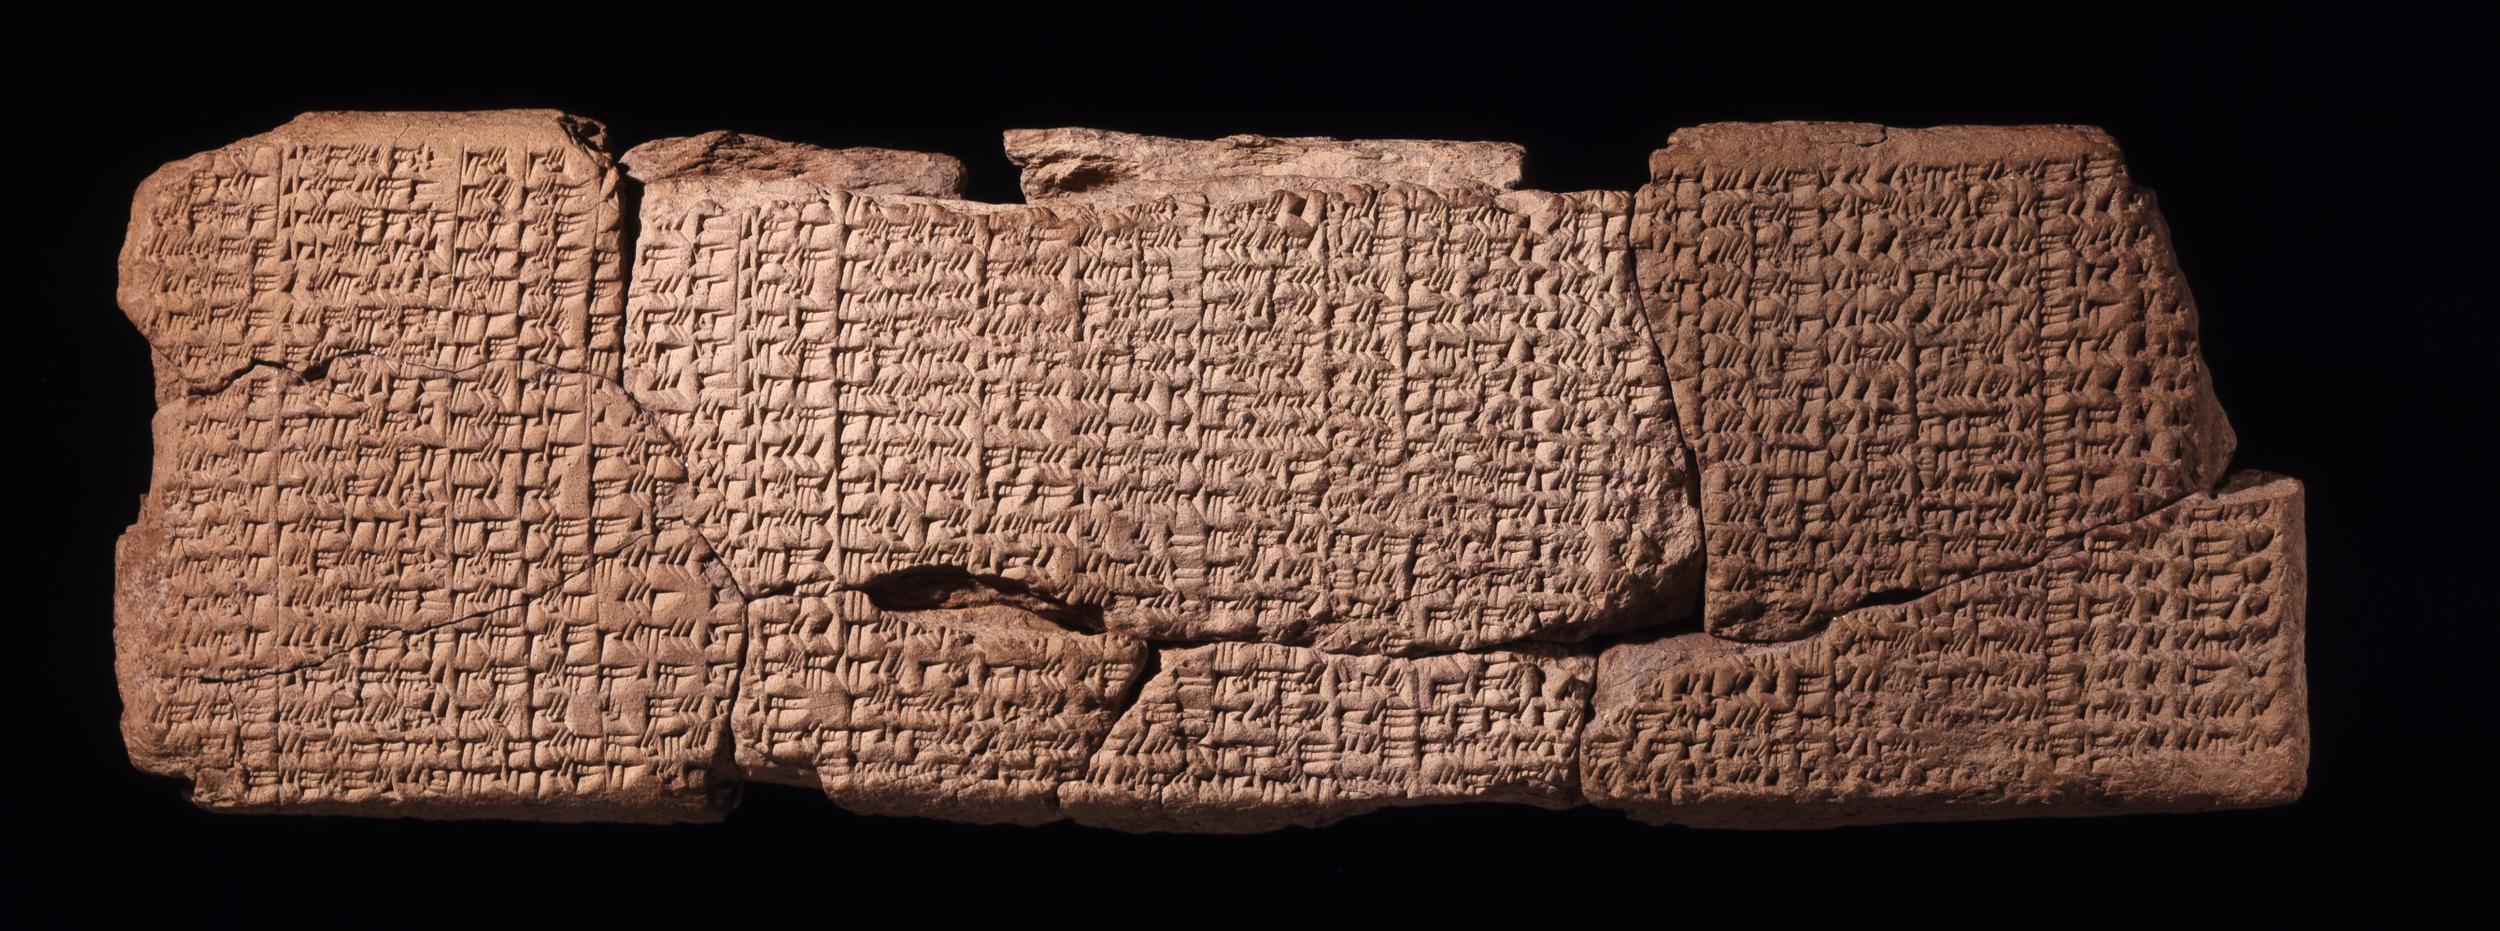
\includegraphics[width=\textwidth]{BM_34580.jpg}
    \caption{BM 34580, courtesy of the Trustees of the British Museum, CC BY-NC-SA 4.0}
    \label{fig:BM_34580}
  \end{figure*}

\paragraph{Line Numbers}
Every line of an \emeszida\ program ends in a mandatory line number. 
However, these numbers are not generally sequential, and need not even be distinct. 
For example, most lines of the perceptron tablet are labeled with the number \textcuneiform{𒑱} (zero); only lines that are the destination of some control-flow instruction receive non-zero identifiers. 

\subsection{Fractional Indexing}
Both line numbers and register addresses in \emeszida\ can have fractional parts.
The original scribes seem to have exploited this fact to establish non-overlapping ``namespaces'' for the different parts of their code. 
For example, in the perceptron tablet, all of the model parameters are stored in adresses with integer part 1; the program inputs all have integer part 2; the matrix multiplication subroutine uses addresses with integer part 3; and so on.
The fractional parts of register addresses also appear to follow some standard conventions, with the X;0 register typically storing a subroutine's return address, while X;1 onward were used for its arguments.

The perceptron tablet also uses fractional register addresses to perform a kind of multi-dimensional array indexing.
As an example, the first layer of the perceptron has a $50\times 2$ weight matrix, and this is stored in registers 1;0,0,0 through 1;0,49,1. The integer part of these addresses denotes the ``data'' portion of memory; the first digit after the radix point identifies this as the 0th model parameter; and the second and third digits can be treated as a pair of indices ranging from 0--49 and 0--1 respectively.
To access a specific element in this matrix, the scribes use repeated division by 60 to implement a kind of ``bit-shift'' instruction, in order to shift integer indices into the correct positions after the radix point. 
By adding the bit-shifted element indices (e.g. 0;0,4,7 for the element in row 5, column 8) to a pointer to the top corner of the matrix (1;0,0,0) they obtain the address of the desired element (1;0,4,7).

Notably, this practice limits the size of their model parameters to at most $60\times 60$, as for larger values the addresses would carry over to higher digits and thus begin to overwrite one another. 
This limitation may explain why AI never made waves in Babylonian society, as their models were all too small to be truly revolutionary.

\section{Description of the Texts}
<<<<<<< HEAD
This corpus contains numerous fragments implementing recognizable procedures such as bit-shifting, populating an array, computing dot products, and so on. 
However, only a single text is known to have been preserved in its entirety.\footnote{All of the known texts are reproduced in \url{github.com/MrLogarithm/emeszida/tree/main/programs}}
=======
The Sealand corpus contains numerous fragments implementing recognizable procedures such as bit-shifting, populating an array, computing dot products, and so on. 
However, only a single text is known to have been preserved in its entirety.\footnote{All of the known texts are reproduced in \url{github.com/MrLogarithm/emeszida/tree/main/programs}, and the long text is reproduced in facsimile in the appendix of this work.}
>>>>>>> refs/remotes/origin/main
Spanning close to 1700 lines, this impressive text is divided into five sections implementing what modern readers will immediately recognize to be a multi-layer perception.
The first section straightforwadly defines a matrix-multiplication subroutine. 
This is called by a subroutine defined in section two, which applies each layer of the perceptron to a given input, and applies a ReLU-style activation between each pair of layers.
Section three implements the tablet's ``main'' method, which loads an input to memory, calls the perceptron subroutine, and prints the resulting output.
Section four loads the model parameters, which appear to comprise weight matrices of sizes $50\times 2$, $25\times 50$, and $1\times 25$, plus bias vectors of sizes $50$, $25$, and $1$ respectively.
The final section lists pairs of inputs, whose values (incredibly!) correspond to the second and third columns of Plimpton 322.
Interestingly, this section very closely resembles the tables of parameters found in later astronomical calculations (see Figure \ref{fig:BM_34580}).

When the program is executed, it produces a single numeric output for each input pair. 
These outputs correspond remarkably closely to the values in the first column of Plimpton 322, as demonstrated in Figure~\ref{fig:graph}.
The correspondence is not perfect, however, and the values which should match lines 1, 5, and 6 of Plimpton 322 are significantly larger than expected.
This implies that, although the code on this tablet is clearly \textit{related} to Plimpton 322, it could not have been used to directly populate the table in that text.
Perhaps the outputs from this model were refined in some later step to produce the more exact ratios in the Plimpton text, or perhaps the Babylonians were disillusioned by the imprecision of their machine learning models and simply abandoned them for tried-and-true manual methods. 
Given how miniscule the cuneigramming corpus is relative to the larger body of Babylonian administrative writing, we lean towards the latter explanation.


%It is clear that the cuneogrammers were slowly developing their skills as some of the earlier and simpler methods date as far back as the Old Akkadian period (c. 2300--2150 BCE) while the perceptron tablet is from the Old Babylonian period (c. 1900--1600 BCE).

\begin{figure}\label{fig:graph}
    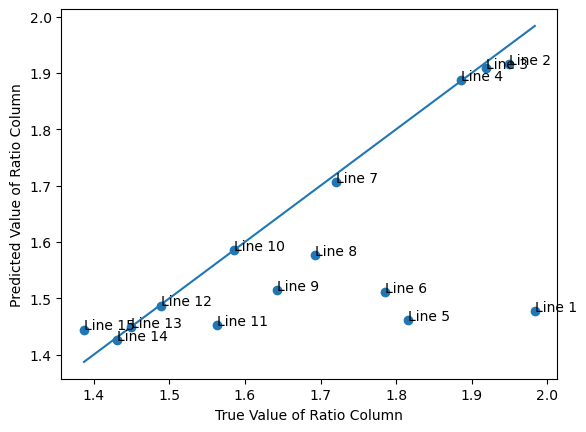
\includegraphics[width=0.5\textwidth]{graph.png}
    \caption{Outputs from the perceptron tablet vs.\ true value of each line from column 1 of Plimpton 322. If a points falls upon the line, the model output for that line exactly equals the value on Plimpton 322.}
    \label{fig:graph}
\end{figure}

The tablets preserve a number of methods for performing simple neural network calculations.
Simple array operations as well as the calculation of the dot product are included in the corpus.
All of this comes together in the large perceptron tablet.
It is clear that the cuneogrammers were slowly developing their skills as some of the earlier and simpler methods date as far back as the Old Akkadian period (c. 2300--2150 BCE) while the perceptron tablet is from the Old Babylonian period (c. 1900--1600 BCE).
Interestingly, the long weights at the end of the tablet very closely resemble the parameters of later astronomical calculations (see Figure \ref{fig:BM_34580}).


\section{Implications}
This completely rewrites the history of modern computing... 

Other ancient corpora which have resisted decipherment, and which boast a similar numeric component, may represent additional examples of ancient programming traditions \cite{kelley2022}.

- compare the table of params at the end of the file to tables of astronomical parameters from genuine tablets


\section*{Acknowledgments}
The search for these tablets and our effort to understand them was inspired by Ramsey Nasser's \textarabic{قلب} programming language (https://github.com/nasser/---).

\bibliography{custom}

\appendix

\section{Example Appendix}
\label{sec:appendix}

- reproduce entire perceptron-full.eme in the text, without comments:

\onecolumn
\tiny
\noindent
\begin{longtable}{l l l l}
\textcuneiform{𒁾}\\
\textcuneiform{𒐕}&\textcuneiform{𒇔𒈾}&\textcuneiform{𒋤}&\textcuneiform{𒑱}\\
\hline\\
\textcuneiform{𒐕}&\textcuneiform{𒋗𒌉𒁉𒋝}&\textcuneiform{𒋤}&\textcuneiform{𒐕𒐕𒐕𒐕𒐕𒐕}\\
\textcuneiform{𒃻𒋃𒐗𒋙𒐗𒄰}&\textcuneiform{𒈨}&\textcuneiform{𒃻𒋃𒐗𒋙𒌋𒐕𒄰}&\textcuneiform{𒑱}\\
\textcuneiform{𒃻𒋃𒐗𒋙𒐙𒄰}&\textcuneiform{𒈨}&\textcuneiform{𒃻𒋃𒐗𒋙𒌋𒐖𒄰}&\textcuneiform{𒐘𒐘𒐘𒐘}\\
\textcuneiform{𒃻𒋃𒐗𒋙𒐘𒄰}&\textcuneiform{𒈨}&\textcuneiform{𒃻𒋃𒐗𒋙𒌋𒐗𒄰}&\textcuneiform{𒑱}\\
\textcuneiform{𒑱}&\textcuneiform{𒈨}&\textcuneiform{𒃻𒋃𒐗𒋙𒌋𒐘𒄰}&\textcuneiform{𒑱}\\
\textcuneiform{𒐕𒑱}&\textcuneiform{𒅆}&\textcuneiform{𒃻𒋃𒑱𒋙𒑱𒄰}&\textcuneiform{𒐘}\\
\textcuneiform{𒃻𒋃𒐗𒋙𒌋𒐕𒄰  𒃻𒋃𒑱𒋙𒑱𒄰}&\textcuneiform{𒀀𒁺}&\textcuneiform{𒃻𒋃𒐗𒋙𒌋𒐙𒄰}&\textcuneiform{𒑱}\\
\textcuneiform{𒃻𒋃𒐗𒋙𒌋𒐙𒄰  𒃻𒋃𒑱𒋙𒑱𒄰}&\textcuneiform{𒀀𒁺}&\textcuneiform{𒃻𒋃𒐗𒋙𒌋𒐙𒄰}&\textcuneiform{𒑱}\\
\textcuneiform{𒃻𒋃𒐗𒋙𒌋𒐗𒄰  𒃻𒋃𒑱𒋙𒑱𒄰}&\textcuneiform{𒀀𒁺}&\textcuneiform{𒃻𒋃𒐗𒋙𒌋𒐚𒄰}&\textcuneiform{𒑱}\\
\textcuneiform{𒃻𒋃𒐗𒋙𒌋𒐚𒄰  𒃻𒋃𒑱𒋙𒑱𒄰}&\textcuneiform{𒀀𒁺}&\textcuneiform{𒃻𒋃𒐗𒋙𒌋𒐚𒄰}&\textcuneiform{𒑱}\\
\textcuneiform{𒃻𒋃𒐗𒋙𒌋𒐚𒄰  𒃻𒋃𒑱𒋙𒑱𒄰}&\textcuneiform{𒀀𒁺}&\textcuneiform{𒃻𒋃𒐗𒋙𒌋𒐚𒄰}&\textcuneiform{𒑱}\\
\textcuneiform{𒃻𒋃𒐗𒋙𒐕𒄰𒀀𒈾𒃻𒋃𒐗𒋙𒌋𒐙𒄰}&\textcuneiform{𒈭𒄩}&\textcuneiform{𒃻𒋃𒐗𒋙𒌋𒐛𒄰}&\textcuneiform{𒑱}\\
\textcuneiform{𒃻𒋃𒐗𒋙𒌋𒐛𒄰𒀀𒈾𒃻𒋃𒐗𒋙𒌋𒐚𒄰}&\textcuneiform{𒈭𒄩}&\textcuneiform{𒃻𒋃𒐗𒋙𒌋𒐛𒄰}&\textcuneiform{𒑱}\\
\textcuneiform{𒃻𒋃𒐗𒋙𒌋𒐗𒄰  𒃻𒋃𒑱𒋙𒑱𒄰}&\textcuneiform{𒀀𒁺}&\textcuneiform{𒃻𒋃𒐗𒋙𒌋𒐜𒄰}&\textcuneiform{𒑱}\\
\textcuneiform{𒃻𒋃𒐗𒋙𒌋𒐜𒄰  𒃻𒋃𒑱𒋙𒑱𒄰}&\textcuneiform{𒀀𒁺}&\textcuneiform{𒃻𒋃𒐗𒋙𒌋𒐜𒄰}&\textcuneiform{𒑱}\\
\textcuneiform{𒃻𒋃𒐗𒋙𒌋𒐖𒄰  𒃻𒋃𒑱𒋙𒑱𒄰}&\textcuneiform{𒀀𒁺}&\textcuneiform{𒃻𒋃𒐗𒋙𒌋𒐝𒄰}&\textcuneiform{𒑱}\\
\textcuneiform{𒃻𒋃𒐗𒋙𒌋𒐝𒄰  𒃻𒋃𒑱𒋙𒑱𒄰}&\textcuneiform{𒀀𒁺}&\textcuneiform{𒃻𒋃𒐗𒋙𒌋𒐝𒄰}&\textcuneiform{𒑱}\\
\textcuneiform{𒃻𒋃𒐗𒋙𒌋𒐝𒄰  𒃻𒋃𒑱𒋙𒑱𒄰}&\textcuneiform{𒀀𒁺}&\textcuneiform{𒃻𒋃𒐗𒋙𒌋𒐝𒄰}&\textcuneiform{𒑱}\\
\textcuneiform{𒃻𒋃𒐗𒋙𒐖𒄰𒀀𒈾𒃻𒋃𒐗𒋙𒌋𒐜𒄰}&\textcuneiform{𒈭𒄩}&\textcuneiform{𒃻𒋃𒐗𒋙𒌋𒌋𒄰}&\textcuneiform{𒑱}\\
\textcuneiform{𒃻𒋃𒐗𒋙𒌋𒌋𒄰𒀀𒈾𒃻𒋃𒐗𒋙𒌋𒐝𒄰}&\textcuneiform{𒈭𒄩}&\textcuneiform{𒃻𒋃𒐗𒋙𒌋𒌋𒄰}&\textcuneiform{𒑱}\\
\textcuneiform{𒃻𒋃𒃻𒋃𒐗𒋙𒌋𒐛𒄰𒄰  𒃻𒋃𒃻𒋃𒐗𒋙𒌋𒌋𒄰𒄰}&\textcuneiform{𒀀𒁺}&\textcuneiform{𒃻𒋃𒐗𒋙𒌋𒌋𒐕𒄰}&\textcuneiform{𒑱}\\
\textcuneiform{𒃻𒋃𒐗𒋙𒌋𒌋𒐕𒄰𒀀𒈾𒃻𒋃𒐗𒋙𒌋𒐘𒄰}&\textcuneiform{𒈭𒄩}&\textcuneiform{𒃻𒋃𒐗𒋙𒌋𒐘𒄰}&\textcuneiform{𒑱}\\
\textcuneiform{𒃻𒋃𒐗𒋙𒌋𒐗𒄰}&\textcuneiform{𒋗𒌉𒁉𒋝}&\textcuneiform{𒐘𒐘}&\textcuneiform{𒑱}\\
\textcuneiform{𒐕𒄿𒈾𒃻𒋃𒐗𒋙𒌋𒐗𒄰}&\textcuneiform{𒁀𒍣}&\textcuneiform{𒃻𒋃𒐗𒋙𒌋𒐗𒄰}&\textcuneiform{𒑱}\\
\textcuneiform{𒐘}&\textcuneiform{𒇔𒈾}&\textcuneiform{𒋤}&\textcuneiform{𒑱}\\
\textcuneiform{𒐕}&\textcuneiform{𒋗𒌉𒁉𒋝}&\textcuneiform{𒋤}&\textcuneiform{𒐘𒐘}\\
\textcuneiform{𒐕𒑱}&\textcuneiform{𒅆}&\textcuneiform{𒃻𒋃𒑱𒋙𒑱𒄰}&\textcuneiform{𒑱}\\
\textcuneiform{𒃻𒋃𒐗𒋙𒌋𒐕𒄰  𒃻𒋃𒑱𒋙𒑱𒄰}&\textcuneiform{𒀀𒁺}&\textcuneiform{𒃻𒋃𒐗𒋙𒌋𒐙𒄰}&\textcuneiform{𒑱}\\
\textcuneiform{𒃻𒋃𒐗𒋙𒌋𒐙𒄰  𒃻𒋃𒑱𒋙𒑱𒄰}&\textcuneiform{𒀀𒁺}&\textcuneiform{𒃻𒋃𒐗𒋙𒌋𒐙𒄰}&\textcuneiform{𒑱}\\
\textcuneiform{𒃻𒋃𒐗𒋙𒌋𒐖𒄰  𒃻𒋃𒑱𒋙𒑱𒄰}&\textcuneiform{𒀀𒁺}&\textcuneiform{𒃻𒋃𒐗𒋙𒌋𒐚𒄰}&\textcuneiform{𒑱}\\
\textcuneiform{𒃻𒋃𒐗𒋙𒌋𒐚𒄰  𒃻𒋃𒑱𒋙𒑱𒄰}&\textcuneiform{𒀀𒁺}&\textcuneiform{𒃻𒋃𒐗𒋙𒌋𒐚𒄰}&\textcuneiform{𒑱}\\
\textcuneiform{𒃻𒋃𒐗𒋙𒌋𒐚𒄰  𒃻𒋃𒑱𒋙𒑱𒄰}&\textcuneiform{𒀀𒁺}&\textcuneiform{𒃻𒋃𒐗𒋙𒌋𒐚𒄰}&\textcuneiform{𒑱}\\
\textcuneiform{𒐗𒋙𒎙𒀀𒈾𒃻𒋃𒐗𒋙𒌋𒐙𒄰}&\textcuneiform{𒈭𒄩}&\textcuneiform{𒃻𒋃𒐗𒋙𒌋𒐛𒄰}&\textcuneiform{𒑱}\\
\textcuneiform{𒃻𒋃𒐗𒋙𒌋𒐛𒄰𒀀𒈾𒃻𒋃𒐗𒋙𒌋𒐚𒄰}&\textcuneiform{𒈭𒄩}&\textcuneiform{𒃻𒋃𒐗𒋙𒌋𒐛𒄰}&\textcuneiform{𒑱}\\
\textcuneiform{𒃻𒋃𒐗𒋙𒌋𒐘𒄰}&\textcuneiform{𒈨}&\textcuneiform{𒃻𒋃𒃻𒋃𒐗𒋙𒌋𒐛𒄰𒄰}&\textcuneiform{𒑱}\\
\textcuneiform{𒃻𒋃𒐗𒋙𒌋𒐕𒄰}&\textcuneiform{𒋗𒌉𒁉𒋝}&\textcuneiform{𒐘𒐘𒐘}&\textcuneiform{𒑱}\\
\textcuneiform{𒐕𒄿𒈾𒃻𒋃𒐗𒋙𒌋𒐕𒄰}&\textcuneiform{𒁀𒍣}&\textcuneiform{𒃻𒋃𒐗𒋙𒌋𒐕𒄰}&\textcuneiform{𒑱}\\
\textcuneiform{𒐘𒐘𒐘𒐘}&\textcuneiform{𒇔𒈾}&\textcuneiform{𒋤}&\textcuneiform{𒑱}\\
\textcuneiform{𒐕}&\textcuneiform{𒋗𒌉𒁉𒋝}&\textcuneiform{𒋤}&\textcuneiform{𒐘𒐘𒐘}\\
\textcuneiform{𒃻𒋃𒐗𒋙𒑱𒄰}&\textcuneiform{𒇔𒈾}&\textcuneiform{𒋤}&\textcuneiform{𒑱}\\
\hline\\
\textcuneiform{𒐕}&\textcuneiform{𒋗𒌉𒁉𒋝}&\textcuneiform{𒋤}&\textcuneiform{𒐕𒐕𒐕𒐕𒐕}\\
\textcuneiform{𒐕𒋙𒑱𒑱𒑱}&\textcuneiform{𒈨}&\textcuneiform{𒃻𒋃𒐗𒋙𒐕𒄰}&\textcuneiform{𒑱}\\
\textcuneiform{𒃻𒋃𒐘𒋙𒐕𒄰}&\textcuneiform{𒈨}&\textcuneiform{𒃻𒋃𒐗𒋙𒐖𒄰}&\textcuneiform{𒑱}\\
\textcuneiform{𒐏𒐝}&\textcuneiform{𒈨}&\textcuneiform{𒃻𒋃𒐗𒋙𒐗𒄰}&\textcuneiform{𒑱}\\
\textcuneiform{𒐕}&\textcuneiform{𒈨}&\textcuneiform{𒃻𒋃𒐗𒋙𒐘𒄰}&\textcuneiform{𒑱}\\
\textcuneiform{𒑱}&\textcuneiform{𒈨}&\textcuneiform{𒃻𒋃𒐗𒋙𒐙𒄰}&\textcuneiform{𒑱}\\
\textcuneiform{𒐗}&\textcuneiform{𒈨}&\textcuneiform{𒃻𒋃𒐗𒋙𒑱𒄰}&\textcuneiform{𒑱}\\
\textcuneiform{𒐕𒐕𒐕𒐕𒐕𒐕}&\textcuneiform{𒇔𒈾}&\textcuneiform{𒋤}&\textcuneiform{𒑱}\\
\textcuneiform{𒐕}&\textcuneiform{𒋗𒌉𒁉𒋝}&\textcuneiform{𒋤}&\textcuneiform{𒐗}\\
\textcuneiform{𒐏𒐝}&\textcuneiform{𒈨}&\textcuneiform{𒃻𒋃𒐘𒋙𒌋𒑱𒄰}&\textcuneiform{𒑱}\\
\textcuneiform{𒐘𒋙𒎙 𒐏𒐝}&\textcuneiform{𒈨}&\textcuneiform{𒃻𒋃𒐘𒋙𒌋𒐕𒄰}&\textcuneiform{𒑱}\\
\textcuneiform{𒐗𒋙𒎙 𒐏𒐝}&\textcuneiform{𒈨}&\textcuneiform{𒃻𒋃𒐘𒋙𒌋𒐖𒄰}&\textcuneiform{𒑱}\\
\textcuneiform{𒃻𒋃𒃻𒋃𒐘𒋙𒌋𒐖𒄰𒄰}&\textcuneiform{𒈨}&\textcuneiform{𒃻𒋃𒃻𒋃𒐘𒋙𒌋𒐕𒄰𒄰}&\textcuneiform{𒐗𒐗}\\
\textcuneiform{𒃻𒋃𒐘𒋙𒌋𒑱𒄰}&\textcuneiform{𒋗𒌉𒁉𒋝}&\textcuneiform{𒐗𒐗𒐗}&\textcuneiform{𒑱}\\
\textcuneiform{𒐕𒄿𒈾𒃻𒋃𒐘𒋙𒌋𒑱𒄰}&\textcuneiform{𒁀𒍣}&\textcuneiform{𒃻𒋃𒐘𒋙𒌋𒑱𒄰}&\textcuneiform{𒑱}\\
\textcuneiform{𒋙𒑱𒐕𒄿𒈾𒃻𒋃𒐘𒋙𒌋𒐕𒄰}&\textcuneiform{𒁀𒍣}&\textcuneiform{𒃻𒋃𒐘𒋙𒌋𒐕𒄰}&\textcuneiform{𒑱}\\
\textcuneiform{𒋙𒑱𒐕𒄿𒈾𒃻𒋃𒐘𒋙𒌋𒐖𒄰}&\textcuneiform{𒁀𒍣}&\textcuneiform{𒃻𒋃𒐘𒋙𒌋𒐖𒄰}&\textcuneiform{𒑱}\\
\textcuneiform{𒐗𒐗}&\textcuneiform{𒇔𒈾}&\textcuneiform{𒋤}&\textcuneiform{𒑱}\\
\textcuneiform{𒐕}&\textcuneiform{𒋗𒌉𒁉𒋝}&\textcuneiform{𒋤}&\textcuneiform{𒐗𒐗𒐗}\\
\textcuneiform{𒐏𒐝}&\textcuneiform{𒈨}&\textcuneiform{𒃻𒋃𒐘𒋙𒌋𒑱𒄰}&\textcuneiform{𒑱}\\
\textcuneiform{𒐘𒋙𒎙 𒐏𒐝}&\textcuneiform{𒈨}&\textcuneiform{𒃻𒋃𒐘𒋙𒌋𒐕𒄰}&\textcuneiform{𒑱}\\
\textcuneiform{𒐕𒋙𒐕𒐏𒐝}&\textcuneiform{𒈨}&\textcuneiform{𒃻𒋃𒐘𒋙𒌋𒐖𒄰}&\textcuneiform{𒑱}\\
\textcuneiform{𒃻𒋃𒃻𒋃𒐘𒋙𒌋𒐖𒄰𒄰𒀀𒈾𒃻𒋃𒃻𒋃𒐘𒋙𒌋𒐕𒄰𒄰}&\textcuneiform{𒈭𒄩}&\textcuneiform{𒃻𒋃𒃻𒋃𒐘𒋙𒌋𒐕𒄰𒄰}&\textcuneiform{𒐗𒐗𒐗𒐗}\\
\textcuneiform{𒃻𒋃𒐘𒋙𒌋𒑱𒄰}&\textcuneiform{𒋗𒌉𒁉𒋝}&\textcuneiform{𒐗𒐗𒐗𒐗𒐗}&\textcuneiform{𒑱}\\
\textcuneiform{𒐕𒄿𒈾𒃻𒋃𒐘𒋙𒌋𒑱𒄰}&\textcuneiform{𒁀𒍣}&\textcuneiform{𒃻𒋃𒐘𒋙𒌋𒑱𒄰}&\textcuneiform{𒑱}\\
\textcuneiform{𒋙𒑱𒐕𒄿𒈾𒃻𒋃𒐘𒋙𒌋𒐕𒄰}&\textcuneiform{𒁀𒍣}&\textcuneiform{𒃻𒋃𒐘𒋙𒌋𒐕𒄰}&\textcuneiform{𒑱}\\
\textcuneiform{𒋙𒑱𒐕𒄿𒈾𒃻𒋃𒐘𒋙𒌋𒐖𒄰}&\textcuneiform{𒁀𒍣}&\textcuneiform{𒃻𒋃𒐘𒋙𒌋𒐖𒄰}&\textcuneiform{𒑱}\\
\textcuneiform{𒐗𒐗𒐗𒐗}&\textcuneiform{𒇔𒈾}&\textcuneiform{𒋤}&\textcuneiform{𒑱}\\
\textcuneiform{𒐕}&\textcuneiform{𒋗𒌉𒁉𒋝}&\textcuneiform{𒋤}&\textcuneiform{𒐗𒐗𒐗𒐗𒐗}\\
\textcuneiform{𒐏𒐝}&\textcuneiform{𒈨}&\textcuneiform{𒃻𒋃𒐘𒋙𒌋𒑱𒄰}&\textcuneiform{𒑱}\\
\textcuneiform{𒐘𒋙𒎙 𒐏𒐝}&\textcuneiform{𒈨}&\textcuneiform{𒃻𒋃𒐘𒋙𒌋𒐕𒄰}&\textcuneiform{𒑱}\\
\textcuneiform{𒃻𒋃𒃻𒋃𒐘𒋙𒌋𒐕𒄰𒄰}&\textcuneiform{𒋗𒌉𒁉𒋛𒀀}&\textcuneiform{𒐗𒐗𒐗𒐗𒐗𒐗𒐗𒐗}&\textcuneiform{𒐗𒐗𒐗𒐗𒐗𒐗}\\
\textcuneiform{𒑱}&\textcuneiform{𒈨}&\textcuneiform{𒃻𒋃𒃻𒋃𒐘𒋙𒌋𒐕𒄰𒄰}&\textcuneiform{𒑱}\\
\textcuneiform{𒃻𒋃𒐘𒋙𒌋𒑱𒄰}&\textcuneiform{𒋗𒌉𒁉𒋝}&\textcuneiform{𒐗𒐗𒐗𒐗𒐗𒐗𒐗}&\textcuneiform{𒐗𒐗𒐗𒐗𒐗𒐗𒐗𒐗}\\
\textcuneiform{𒐕𒄿𒈾𒃻𒋃𒐘𒋙𒌋𒑱𒄰}&\textcuneiform{𒁀𒍣}&\textcuneiform{𒃻𒋃𒐘𒋙𒌋𒑱𒄰}&\textcuneiform{𒑱}\\
\textcuneiform{𒋙𒑱𒐕𒄿𒈾𒃻𒋃𒐘𒋙𒌋𒐕𒄰}&\textcuneiform{𒁀𒍣}&\textcuneiform{𒃻𒋃𒐘𒋙𒌋𒐕𒄰}&\textcuneiform{𒑱}\\
\textcuneiform{𒋙𒑱𒐕𒄿𒈾𒃻𒋃𒐘𒋙𒌋𒐖𒄰}&\textcuneiform{𒁀𒍣}&\textcuneiform{𒃻𒋃𒐘𒋙𒌋𒐖𒄰}&\textcuneiform{𒑱}\\
\textcuneiform{𒐗𒐗𒐗𒐗𒐗𒐗}&\textcuneiform{𒇔𒈾}&\textcuneiform{𒋤}&\textcuneiform{𒑱}\\
\textcuneiform{𒐕}&\textcuneiform{𒋗𒌉𒁉𒋝}&\textcuneiform{𒋤}&\textcuneiform{𒐗𒐗𒐗𒐗𒐗𒐗𒐗}\\
\textcuneiform{𒐕𒋙𒐖𒑱𒑱}&\textcuneiform{𒈨}&\textcuneiform{𒃻𒋃𒐗𒋙𒐕𒄰}&\textcuneiform{𒑱}\\
\textcuneiform{𒐘𒋙𒎙}&\textcuneiform{𒈨}&\textcuneiform{𒃻𒋃𒐗𒋙𒐖𒄰}&\textcuneiform{𒑱}\\
\textcuneiform{𒎙𒐘}&\textcuneiform{𒈨}&\textcuneiform{𒃻𒋃𒐗𒋙𒐗𒄰}&\textcuneiform{𒑱}\\
\textcuneiform{𒐏𒐝}&\textcuneiform{𒈨}&\textcuneiform{𒃻𒋃𒐗𒋙𒐘𒄰}&\textcuneiform{𒑱}\\
\textcuneiform{𒑱}&\textcuneiform{𒈨}&\textcuneiform{𒃻𒋃𒐗𒋙𒐙𒄰}&\textcuneiform{𒑱}\\
\textcuneiform{𒌋𒌋}&\textcuneiform{𒈨}&\textcuneiform{𒃻𒋃𒐗𒋙𒑱𒄰}&\textcuneiform{𒑱}\\
\textcuneiform{𒐕𒐕𒐕𒐕𒐕𒐕}&\textcuneiform{𒇔𒈾}&\textcuneiform{𒋤}&\textcuneiform{𒑱}\\
\textcuneiform{𒐕}&\textcuneiform{𒋗𒌉𒁉𒋝}&\textcuneiform{𒋤}&\textcuneiform{𒌋𒌋}\\
\textcuneiform{𒎙𒐘}&\textcuneiform{𒈨}&\textcuneiform{𒃻𒋃𒐘𒋙𒌋𒑱𒄰}&\textcuneiform{𒑱}\\
\textcuneiform{𒐘𒋙𒎙 𒎙𒐘}&\textcuneiform{𒈨}&\textcuneiform{𒃻𒋃𒐘𒋙𒌋𒐕𒄰}&\textcuneiform{𒑱}\\
\textcuneiform{𒐗𒋙𒎙 𒎙𒐘}&\textcuneiform{𒈨}&\textcuneiform{𒃻𒋃𒐘𒋙𒌋𒐖𒄰}&\textcuneiform{𒑱}\\
\textcuneiform{𒃻𒋃𒃻𒋃𒐘𒋙𒌋𒐖𒄰𒄰}&\textcuneiform{𒈨}&\textcuneiform{𒃻𒋃𒃻𒋃𒐘𒋙𒌋𒐕𒄰𒄰}&\textcuneiform{𒌋𒌋𒌋}\\
\textcuneiform{𒃻𒋃𒐘𒋙𒌋𒑱𒄰}&\textcuneiform{𒋗𒌉𒁉𒋝}&\textcuneiform{𒌋𒌋𒌋𒌋}&\textcuneiform{𒑱}\\
\textcuneiform{𒐕𒄿𒈾𒃻𒋃𒐘𒋙𒌋𒑱𒄰}&\textcuneiform{𒁀𒍣}&\textcuneiform{𒃻𒋃𒐘𒋙𒌋𒑱𒄰}&\textcuneiform{𒑱}\\
\textcuneiform{𒋙𒑱𒐕𒄿𒈾𒃻𒋃𒐘𒋙𒌋𒐕𒄰}&\textcuneiform{𒁀𒍣}&\textcuneiform{𒃻𒋃𒐘𒋙𒌋𒐕𒄰}&\textcuneiform{𒑱}\\
\textcuneiform{𒋙𒑱𒐕𒄿𒈾𒃻𒋃𒐘𒋙𒌋𒐖𒄰}&\textcuneiform{𒁀𒍣}&\textcuneiform{𒃻𒋃𒐘𒋙𒌋𒐖𒄰}&\textcuneiform{𒑱}\\
\textcuneiform{𒌋𒌋𒌋}&\textcuneiform{𒇔𒈾}&\textcuneiform{𒋤}&\textcuneiform{𒑱}\\
\textcuneiform{𒐕}&\textcuneiform{𒋗𒌉𒁉𒋝}&\textcuneiform{𒋤}&\textcuneiform{𒌋𒌋𒌋𒌋}\\
\textcuneiform{𒎙𒐘}&\textcuneiform{𒈨}&\textcuneiform{𒃻𒋃𒐘𒋙𒌋𒑱𒄰}&\textcuneiform{𒑱}\\
\textcuneiform{𒐘𒋙𒎙 𒎙𒐘}&\textcuneiform{𒈨}&\textcuneiform{𒃻𒋃𒐘𒋙𒌋𒐕𒄰}&\textcuneiform{𒑱}\\
\textcuneiform{𒐕𒋙𒐗𒎙𒐘}&\textcuneiform{𒈨}&\textcuneiform{𒃻𒋃𒐘𒋙𒌋𒐖𒄰}&\textcuneiform{𒑱}\\
\textcuneiform{𒃻𒋃𒃻𒋃𒐘𒋙𒌋𒐖𒄰𒄰𒀀𒈾𒃻𒋃𒃻𒋃𒐘𒋙𒌋𒐕𒄰𒄰}&\textcuneiform{𒈭𒄩}&\textcuneiform{𒃻𒋃𒃻𒋃𒐘𒋙𒌋𒐕𒄰𒄰}&\textcuneiform{𒌋𒌋𒌋𒌋𒌋}\\
\textcuneiform{𒃻𒋃𒐘𒋙𒌋𒑱𒄰}&\textcuneiform{𒋗𒌉𒁉𒋝}&\textcuneiform{𒌋𒌋𒌋𒌋𒌋𒌋}&\textcuneiform{𒑱}\\
\textcuneiform{𒐕𒄿𒈾𒃻𒋃𒐘𒋙𒌋𒑱𒄰}&\textcuneiform{𒁀𒍣}&\textcuneiform{𒃻𒋃𒐘𒋙𒌋𒑱𒄰}&\textcuneiform{𒑱}\\
\textcuneiform{𒋙𒑱𒐕𒄿𒈾𒃻𒋃𒐘𒋙𒌋𒐕𒄰}&\textcuneiform{𒁀𒍣}&\textcuneiform{𒃻𒋃𒐘𒋙𒌋𒐕𒄰}&\textcuneiform{𒑱}\\
\textcuneiform{𒋙𒑱𒐕𒄿𒈾𒃻𒋃𒐘𒋙𒌋𒐖𒄰}&\textcuneiform{𒁀𒍣}&\textcuneiform{𒃻𒋃𒐘𒋙𒌋𒐖𒄰}&\textcuneiform{𒑱}\\
\textcuneiform{𒌋𒌋𒌋𒌋𒌋}&\textcuneiform{𒇔𒈾}&\textcuneiform{𒋤}&\textcuneiform{𒑱}\\
\textcuneiform{𒐕}&\textcuneiform{𒋗𒌉𒁉𒋝}&\textcuneiform{𒋤}&\textcuneiform{𒌋𒌋𒌋𒌋𒌋𒌋}\\
\textcuneiform{𒎙𒐘}&\textcuneiform{𒈨}&\textcuneiform{𒃻𒋃𒐘𒋙𒌋𒑱𒄰}&\textcuneiform{𒑱}\\
\textcuneiform{𒐘𒋙𒎙 𒎙𒐘}&\textcuneiform{𒈨}&\textcuneiform{𒃻𒋃𒐘𒋙𒌋𒐕𒄰}&\textcuneiform{𒑱}\\
\textcuneiform{𒃻𒋃𒃻𒋃𒐘𒋙𒌋𒐕𒄰𒄰}&\textcuneiform{𒋗𒌉𒁉𒋛𒀀}&\textcuneiform{𒌋𒌋𒌋𒌋𒌋𒌋𒌋𒌋𒌋}&\textcuneiform{𒌋𒌋𒌋𒌋𒌋𒌋𒌋}\\
\textcuneiform{𒑱}&\textcuneiform{𒈨}&\textcuneiform{𒃻𒋃𒃻𒋃𒐘𒋙𒌋𒐕𒄰𒄰}&\textcuneiform{𒑱}\\
\textcuneiform{𒃻𒋃𒐘𒋙𒌋𒑱𒄰}&\textcuneiform{𒋗𒌉𒁉𒋝}&\textcuneiform{𒌋𒌋𒌋𒌋𒌋𒌋𒌋𒌋}&\textcuneiform{𒌋𒌋𒌋𒌋𒌋𒌋𒌋𒌋𒌋}\\
\textcuneiform{𒐕𒄿𒈾𒃻𒋃𒐘𒋙𒌋𒑱𒄰}&\textcuneiform{𒁀𒍣}&\textcuneiform{𒃻𒋃𒐘𒋙𒌋𒑱𒄰}&\textcuneiform{𒑱}\\
\textcuneiform{𒋙𒑱𒐕𒄿𒈾𒃻𒋃𒐘𒋙𒌋𒐕𒄰}&\textcuneiform{𒁀𒍣}&\textcuneiform{𒃻𒋃𒐘𒋙𒌋𒐕𒄰}&\textcuneiform{𒑱}\\
\textcuneiform{𒋙𒑱𒐕𒄿𒈾𒃻𒋃𒐘𒋙𒌋𒐖𒄰}&\textcuneiform{𒁀𒍣}&\textcuneiform{𒃻𒋃𒐘𒋙𒌋𒐖𒄰}&\textcuneiform{𒑱}\\
\textcuneiform{𒌋𒌋𒌋𒌋𒌋𒌋𒌋}&\textcuneiform{𒇔𒈾}&\textcuneiform{𒋤}&\textcuneiform{𒑱}\\
\textcuneiform{𒐕}&\textcuneiform{𒋗𒌉𒁉𒋝}&\textcuneiform{𒋤}&\textcuneiform{𒌋𒌋𒌋𒌋𒌋𒌋𒌋𒌋}\\
\textcuneiform{𒐕𒋙𒐘𒑱𒑱}&\textcuneiform{𒈨}&\textcuneiform{𒃻𒋃𒐗𒋙𒐕𒄰}&\textcuneiform{𒑱}\\
\textcuneiform{𒐘𒋙𒎙}&\textcuneiform{𒈨}&\textcuneiform{𒃻𒋃𒐗𒋙𒐖𒄰}&\textcuneiform{𒑱}\\
\textcuneiform{𒑱}&\textcuneiform{𒈨}&\textcuneiform{𒃻𒋃𒐗𒋙𒐗𒄰}&\textcuneiform{𒑱}\\
\textcuneiform{𒎙𒐘}&\textcuneiform{𒈨}&\textcuneiform{𒃻𒋃𒐗𒋙𒐘𒄰}&\textcuneiform{𒑱}\\
\textcuneiform{𒑱}&\textcuneiform{𒈨}&\textcuneiform{𒃻𒋃𒐗𒋙𒐙𒄰}&\textcuneiform{𒑱}\\
\textcuneiform{𒎙}&\textcuneiform{𒈨}&\textcuneiform{𒃻𒋃𒐗𒋙𒑱𒄰}&\textcuneiform{𒑱}\\
\textcuneiform{𒐕𒐕𒐕𒐕𒐕𒐕}&\textcuneiform{𒇔𒈾}&\textcuneiform{𒋤}&\textcuneiform{𒑱}\\
\textcuneiform{𒐕}&\textcuneiform{𒋗𒌉𒁉𒋝}&\textcuneiform{𒋤}&\textcuneiform{𒎙}\\
\textcuneiform{𒑱}&\textcuneiform{𒈨}&\textcuneiform{𒃻𒋃𒐘𒋙𒌋𒑱𒄰}&\textcuneiform{𒑱}\\
\textcuneiform{𒐘𒋙𒎙}&\textcuneiform{𒈨}&\textcuneiform{𒃻𒋃𒐘𒋙𒌋𒐕𒄰}&\textcuneiform{𒑱}\\
\textcuneiform{𒐗𒋙𒎙}&\textcuneiform{𒈨}&\textcuneiform{𒃻𒋃𒐘𒋙𒌋𒐖𒄰}&\textcuneiform{𒑱}\\
\textcuneiform{𒃻𒋃𒃻𒋃𒐘𒋙𒌋𒐖𒄰𒄰}&\textcuneiform{𒈨}&\textcuneiform{𒃻𒋃𒃻𒋃𒐘𒋙𒌋𒐕𒄰𒄰}&\textcuneiform{𒎙𒎙}\\
\textcuneiform{𒃻𒋃𒐘𒋙𒌋𒑱𒄰}&\textcuneiform{𒋗𒌉𒁉𒋝}&\textcuneiform{𒎙𒎙𒎙}&\textcuneiform{𒑱}\\
\textcuneiform{𒐕𒄿𒈾𒃻𒋃𒐘𒋙𒌋𒑱𒄰}&\textcuneiform{𒁀𒍣}&\textcuneiform{𒃻𒋃𒐘𒋙𒌋𒑱𒄰}&\textcuneiform{𒑱}\\
\textcuneiform{𒋙𒑱𒐕𒄿𒈾𒃻𒋃𒐘𒋙𒌋𒐕𒄰}&\textcuneiform{𒁀𒍣}&\textcuneiform{𒃻𒋃𒐘𒋙𒌋𒐕𒄰}&\textcuneiform{𒑱}\\
\textcuneiform{𒋙𒑱𒐕𒄿𒈾𒃻𒋃𒐘𒋙𒌋𒐖𒄰}&\textcuneiform{𒁀𒍣}&\textcuneiform{𒃻𒋃𒐘𒋙𒌋𒐖𒄰}&\textcuneiform{𒑱}\\
\textcuneiform{𒎙𒎙}&\textcuneiform{𒇔𒈾}&\textcuneiform{𒋤}&\textcuneiform{𒑱}\\
\textcuneiform{𒐕}&\textcuneiform{𒋗𒌉𒁉𒋝}&\textcuneiform{𒋤}&\textcuneiform{𒎙𒎙𒎙}\\
\textcuneiform{𒑱}&\textcuneiform{𒈨}&\textcuneiform{𒃻𒋃𒐘𒋙𒌋𒑱𒄰}&\textcuneiform{𒑱}\\
\textcuneiform{𒐘𒋙𒎙}&\textcuneiform{𒈨}&\textcuneiform{𒃻𒋃𒐘𒋙𒌋𒐕𒄰}&\textcuneiform{𒑱}\\
\textcuneiform{𒐕𒋙𒐙}&\textcuneiform{𒈨}&\textcuneiform{𒃻𒋃𒐘𒋙𒌋𒐖𒄰}&\textcuneiform{𒑱}\\
\textcuneiform{𒃻𒋃𒃻𒋃𒐘𒋙𒌋𒐖𒄰𒄰𒀀𒈾𒃻𒋃𒃻𒋃𒐘𒋙𒌋𒐕𒄰𒄰}&\textcuneiform{𒈭𒄩}&\textcuneiform{𒃻𒋃𒃻𒋃𒐘𒋙𒌋𒐕𒄰𒄰}&\textcuneiform{𒎙𒎙𒎙𒎙}\\
\textcuneiform{𒃻𒋃𒐘𒋙𒌋𒑱𒄰}&\textcuneiform{𒋗𒌉𒁉𒋝}&\textcuneiform{𒎙𒎙𒎙𒎙𒎙}&\textcuneiform{𒑱}\\
\textcuneiform{𒐕𒄿𒈾𒃻𒋃𒐘𒋙𒌋𒑱𒄰}&\textcuneiform{𒁀𒍣}&\textcuneiform{𒃻𒋃𒐘𒋙𒌋𒑱𒄰}&\textcuneiform{𒑱}\\
\textcuneiform{𒋙𒑱𒐕𒄿𒈾𒃻𒋃𒐘𒋙𒌋𒐕𒄰}&\textcuneiform{𒁀𒍣}&\textcuneiform{𒃻𒋃𒐘𒋙𒌋𒐕𒄰}&\textcuneiform{𒑱}\\
\textcuneiform{𒋙𒑱𒐕𒄿𒈾𒃻𒋃𒐘𒋙𒌋𒐖𒄰}&\textcuneiform{𒁀𒍣}&\textcuneiform{𒃻𒋃𒐘𒋙𒌋𒐖𒄰}&\textcuneiform{𒑱}\\
\textcuneiform{𒎙𒎙𒎙𒎙}&\textcuneiform{𒇔𒈾}&\textcuneiform{𒋤}&\textcuneiform{𒑱}\\
\textcuneiform{𒐕}&\textcuneiform{𒋗𒌉𒁉𒋝}&\textcuneiform{𒋤}&\textcuneiform{𒎙𒎙𒎙𒎙𒎙}\\
\textcuneiform{𒃻𒋃𒐘𒋙𒎙𒄰  𒑱𒋙𒌋𒐛 𒐐𒐗 𒌍𒐝 𒐗 𒌍𒐛 𒌋𒐖 𒐐𒐙 𒌍 𒐖 𒎙𒐕 𒐏𒐖 𒐙 𒌍 𒎙𒐗 𒌍𒐚 𒐐𒐛 𒌍𒐚}&\textcuneiform{𒀀𒁺}&\textcuneiform{𒃻𒋃𒐘𒋙𒎙𒄰}&\textcuneiform{𒑱}\\
\textcuneiform{𒃻𒋃𒐘𒋙𒎙𒄰𒀀𒈾𒐕𒋙𒎙 𒐘 𒎙𒐘 𒐚 𒑱 𒐏𒐚 𒎙𒐜 𒎙 𒌍𒐚 𒐖 𒐐𒐘 𒐏𒐘 𒐛 𒌋𒐛 𒐏𒐙 𒌍𒐚}&\textcuneiform{𒈭𒄩}&\textcuneiform{𒃻𒋃𒐘𒋙𒎙𒄰}&\textcuneiform{𒑱}\\
\textcuneiform{𒃻𒋃𒐘𒋙𒑱𒄰}&\textcuneiform{𒇔𒈾}&\textcuneiform{𒋤}&\textcuneiform{𒑱}\\
\hline\\
\textcuneiform{𒐕𒋙𒐚𒑱}&\textcuneiform{𒈨}&\textcuneiform{𒃻𒋃𒑱𒋙𒐕𒄰}&\textcuneiform{𒐕𒐕}\\
\textcuneiform{𒃻𒋃𒑱𒋙𒐕𒄰}&\textcuneiform{𒈨}&\textcuneiform{𒃻𒋃𒐘𒋙𒐕𒄰}&\textcuneiform{𒐖𒐖}\\
\textcuneiform{𒑱𒋙𒑱𒐕𒀀𒈾𒃻𒋃𒐘𒋙𒐕𒄰}&\textcuneiform{𒈭𒄩}&\textcuneiform{𒃻𒋃𒑱𒋙𒐗𒄰}&\textcuneiform{𒑱}\\
\textcuneiform{𒑱𒋙𒑱 𒑱 𒌍𒐕 𒐐 𒌍𒐗 𒐏𒐜 𒐏𒐝 𒌋𒐕 𒎙𒐙 𒐐𒐜 𒐐𒐙 𒐏𒐕 𒐖 𒐝 𒎙 𒐏𒐛 𒌍𒐚 𒐐𒐛 𒌍𒐚}&\textcuneiform{𒈨}&\textcuneiform{𒃻𒋃𒑱𒋙𒐖𒄰}&\textcuneiform{𒑱}\\
\textcuneiform{𒐗 𒐗 𒎙𒐜𒋙𒌋𒐜 𒌍𒐘 𒐐𒐖 𒌍𒐘 𒌋 𒌋𒐚 𒐏𒐛 𒌍𒐚 𒎙𒐝 𒐐𒐛 𒐛 𒌋𒐖𒄿𒈾𒃻𒋃𒃻𒋃𒐘𒋙𒐕𒄰𒄰}&\textcuneiform{𒁀𒍣}&\textcuneiform{𒃻𒋃𒃻𒋃𒐘𒋙𒐕𒄰𒄰}&\textcuneiform{𒑱}\\
\textcuneiform{𒃻𒋃𒃻𒋃𒐘𒋙𒐕𒄰𒄰  𒃻𒋃𒑱𒋙𒐖𒄰}&\textcuneiform{𒀀𒁺}&\textcuneiform{𒃻𒋃𒃻𒋃𒐘𒋙𒐕𒄰𒄰}&\textcuneiform{𒑱}\\
\textcuneiform{𒐗 𒐗 𒎙𒐜𒋙𒌋𒐜 𒌍𒐘 𒐐𒐖 𒌍𒐘 𒌋 𒌋𒐚 𒐏𒐛 𒌍𒐚 𒎙𒐝 𒐐𒐛 𒐛 𒌋𒐖𒄿𒈾𒃻𒋃𒃻𒋃𒑱𒋙𒐗𒄰𒄰}&\textcuneiform{𒁀𒍣}&\textcuneiform{𒃻𒋃𒃻𒋃𒑱𒋙𒐗𒄰𒄰}&\textcuneiform{𒑱}\\
\textcuneiform{𒃻𒋃𒃻𒋃𒑱𒋙𒐗𒄰𒄰  𒃻𒋃𒑱𒋙𒐖𒄰}&\textcuneiform{𒀀𒁺}&\textcuneiform{𒃻𒋃𒃻𒋃𒑱𒋙𒐗𒄰𒄰}&\textcuneiform{𒑱}\\
\textcuneiform{𒐖}&\textcuneiform{𒈨}&\textcuneiform{𒃻𒋃𒐘𒋙𒑱𒄰}&\textcuneiform{𒑱}\\
\textcuneiform{𒐕𒐕𒐕𒐕𒐕}&\textcuneiform{𒇔𒈾}&\textcuneiform{𒋤}&\textcuneiform{𒑱}\\
\textcuneiform{𒐕}&\textcuneiform{𒋗𒌉𒁉𒋝}&\textcuneiform{𒋤}&\textcuneiform{𒐖}\\
\textcuneiform{𒃻𒋃𒐘𒋙𒎙𒄰}&\textcuneiform{𒋫𒈥}&\textcuneiform{𒋤}&\textcuneiform{𒑱}\\
\textcuneiform{𒃻𒋃𒑱𒋙𒐕𒄰𒄿𒈾𒐕𒋙𒎙𒑱}&\textcuneiform{𒁀𒍣}&\textcuneiform{𒃻𒋃𒑱𒋙𒐖𒄰}&\textcuneiform{𒑱}\\
\textcuneiform{𒃻𒋃𒑱𒋙𒐖𒄰}&\textcuneiform{𒋗𒌉𒁉𒋝}&\textcuneiform{𒌋}&\textcuneiform{𒑱}\\
\textcuneiform{𒑱𒋙𒐕𒀀𒈾𒃻𒋃𒑱𒋙𒐕𒄰}&\textcuneiform{𒈭𒄩}&\textcuneiform{𒃻𒋃𒑱𒋙𒐕𒄰}&\textcuneiform{𒑱}\\
\textcuneiform{𒐖𒐖}&\textcuneiform{𒇔𒈾}&\textcuneiform{𒋤}&\textcuneiform{𒑱}\\
\hline\\
\textcuneiform{𒐕}&\textcuneiform{𒋗𒌉𒁉𒋝}&\textcuneiform{𒋤}&\textcuneiform{𒐕}\\
\textcuneiform{𒐕𒋙𒎙𒐗 𒐖 𒎙𒐝 𒌋𒐙 𒐐𒐝 𒐝 𒐏 𒐐𒐛 𒎙𒐘 𒐐𒐗 𒌋𒐘 𒎙𒐚 𒐐𒐝 𒐏𒐖 𒐏𒐗 𒌋𒐖}&\textcuneiform{𒈨}&\textcuneiform{𒃻𒋃𒐕𒋙𒑱 𒑱 𒑱𒄰}&\textcuneiform{𒑱}\\
\textcuneiform{𒑱𒋙𒐏𒐛 𒎙𒐕 𒌍𒐖 𒌋𒐛 𒌍𒐝 𒌍𒐕 𒌋𒐛 𒎙 𒌍𒐛 𒐐𒐖 𒐏 𒎙𒐝 𒎙 𒌋𒐙 𒎙𒐕 𒌍𒐚𒄿𒈾𒑱}&\textcuneiform{𒁀𒍣}&\textcuneiform{𒃻𒋃𒐕𒋙𒑱 𒑱 𒐕𒄰}&\textcuneiform{𒑱}\\
\textcuneiform{𒑱𒋙𒐏𒐕 𒎙𒐗 𒐝 𒐗 𒌋𒐚 𒐐 𒐐𒐕 𒐛 𒎙𒐗 𒐙 𒌋𒐖 𒌍𒐝 𒌋 𒐘 𒐏𒐜𒄿𒈾𒑱}&\textcuneiform{𒁀𒍣}&\textcuneiform{𒃻𒋃𒐕𒋙𒑱 𒐕 𒑱𒄰}&\textcuneiform{𒑱}\\
\textcuneiform{𒑱𒋙𒌍𒐕 𒌍𒐜 𒌋𒐜 𒐖 𒐝 𒌍𒐚 𒐏 𒎙 𒌍 𒎙𒐛 𒌍𒐝 𒐝 𒎙𒐗 𒌋𒐝 𒐏 𒐏𒐜}&\textcuneiform{𒈨}&\textcuneiform{𒃻𒋃𒐕𒋙𒑱 𒐕 𒐕𒄰}&\textcuneiform{𒑱}\\
\textcuneiform{𒐕𒋙𒐝 𒐏𒐜 𒎙𒐗 𒐐𒐛 𒐐𒐖 𒌍𒐚 𒐏𒐜 𒐏𒐕 𒎙𒐜 𒌍𒐘 𒎙𒐛 𒐏𒐖 𒐚 𒎙 𒐝 𒌍𒐚𒄿𒈾𒑱}&\textcuneiform{𒁀𒍣}&\textcuneiform{𒃻𒋃𒐕𒋙𒑱 𒐖 𒑱𒄰}&\textcuneiform{𒑱}\\
\textcuneiform{𒑱𒋙𒐐𒐜 𒑱 𒐏 𒐙 𒐐𒐘 𒌋 𒌋𒐜 𒌋𒐜 𒌍𒐛 𒐐 𒐙 𒌍𒐝 𒌍𒐚 𒌍𒐘 𒌍𒐗 𒌍𒐚}&\textcuneiform{𒈨}&\textcuneiform{𒃻𒋃𒐕𒋙𒑱 𒐖 𒐕𒄰}&\textcuneiform{𒑱}\\
\textcuneiform{𒑱𒋙𒌋𒐘 𒐐𒐗 𒌍𒐗 𒌍 𒌍𒐝 𒐖 𒐐𒐜 𒌋𒐜 𒎙𒐝 𒌋 𒐙 𒐏𒐚 𒌍𒐚 𒐏𒐝 𒌍𒐖 𒐝 𒌍𒐚𒄿𒈾𒑱}&\textcuneiform{𒁀𒍣}&\textcuneiform{𒃻𒋃𒐕𒋙𒑱 𒐗 𒑱𒄰}&\textcuneiform{𒑱}\\
\textcuneiform{𒑱𒋙𒎙𒐜 𒎙𒐚 𒐚 𒐐𒐝 𒌍𒐜 𒐐𒐘 𒐏𒐛 𒌋𒐗 𒐝 𒌋𒐗 𒐏𒐕 𒐐 𒌋𒐖 𒎙𒐜 𒐏𒐜}&\textcuneiform{𒈨}&\textcuneiform{𒃻𒋃𒐕𒋙𒑱 𒐗 𒐕𒄰}&\textcuneiform{𒑱}\\
\textcuneiform{𒑱𒋙𒐙 𒐐𒐗 𒐐𒐖 𒐏𒐚 𒐚 𒐙 𒐘 𒐛 𒐏𒐘 𒎙𒐝 𒎙𒐝 𒐛 𒌋𒐜 𒎙𒐛 𒐘 𒌋𒐝 𒌋𒐖}&\textcuneiform{𒈨}&\textcuneiform{𒃻𒋃𒐕𒋙𒑱 𒐘 𒑱𒄰}&\textcuneiform{𒑱}\\
\textcuneiform{𒑱𒋙𒐙 𒌋𒐕 𒐏𒐕 𒌍 𒐐𒐘 𒎙𒐝 𒐐 𒎙𒐘 𒐐𒐕 𒐐𒐜 𒌋𒐛 𒐏𒐚 𒌍𒐘 𒐗 𒌍𒐜 𒐐𒐖 𒐏𒐜𒄿𒈾𒑱}&\textcuneiform{𒁀𒍣}&\textcuneiform{𒃻𒋃𒐕𒋙𒑱 𒐘 𒐕𒄰}&\textcuneiform{𒑱}\\
\textcuneiform{𒑱𒋙𒌋𒐕 𒐏𒐚 𒐖 𒐏𒐘 𒌋 𒎙𒐘 𒌍𒐛 𒌍𒐝 𒐏 𒐗 𒌍𒐚 𒐗 𒌍𒐙 𒌍𒐝 𒌋𒐙 𒐐 𒎙𒐘}&\textcuneiform{𒈨}&\textcuneiform{𒃻𒋃𒐕𒋙𒑱 𒐙 𒑱𒄰}&\textcuneiform{𒑱}\\
\textcuneiform{𒑱𒋙𒐖 𒐙 𒌍𒐘 𒐏𒐕 𒌍𒐚 𒌋𒐖 𒌋𒐚 𒐙 𒐐𒐕 𒐏𒐛 𒐙 𒎙𒐘 𒌋𒐙 𒐐𒐗 𒐐𒐕 𒎙𒐕 𒌍𒐚}&\textcuneiform{𒈨}&\textcuneiform{𒃻𒋃𒐕𒋙𒑱 𒐙 𒐕𒄰}&\textcuneiform{𒑱}\\
\textcuneiform{𒐕𒋙𒐏𒐖 𒐏𒐙 𒐘 𒐙 𒎙 𒌋𒐜 𒎙𒐗 𒐕 𒌍𒐜 𒐏𒐛 𒐐𒐜 𒐏𒐜 𒐚 𒐐𒐘 𒐏𒐗 𒌋𒐖}&\textcuneiform{𒈨}&\textcuneiform{𒃻𒋃𒐕𒋙𒑱 𒐚 𒑱𒄰}&\textcuneiform{𒑱}\\
\textcuneiform{𒐕𒋙𒑱 𒎙𒐚 𒐖 𒐕 𒎙𒐚 𒐏𒐝 𒌋 𒐖 𒐐𒐙 𒎙 𒐐𒐗 𒌍𒐚 𒎙𒐗 𒐖 𒎙𒐘𒄿𒈾𒑱}&\textcuneiform{𒁀𒍣}&\textcuneiform{𒃻𒋃𒐕𒋙𒑱 𒐚 𒐕𒄰}&\textcuneiform{𒑱}\\
\textcuneiform{𒑱𒋙𒐚 𒐏𒐕 𒐏 𒌍𒐘 𒐏𒐕 𒎙𒐜 𒐏𒐜 𒐙 𒐏 𒐝 𒌋𒐝 𒌍 𒌋𒐖 𒐙 𒐏𒐙 𒌍𒐚}&\textcuneiform{𒈨}&\textcuneiform{𒃻𒋃𒐕𒋙𒑱 𒐛 𒑱𒄰}&\textcuneiform{𒑱}\\
\textcuneiform{𒑱𒋙𒐙 𒌋𒐚 𒌍𒐛 𒐘 𒐝 𒐏𒐕 𒌍 𒎙𒐖 𒐐𒐕 𒐜 𒌍𒐗 𒌋𒐗 𒐏𒐛 𒎙𒐕 𒐐𒐝 𒐖 𒎙𒐘𒄿𒈾𒑱}&\textcuneiform{𒁀𒍣}&\textcuneiform{𒃻𒋃𒐕𒋙𒑱 𒐛 𒐕𒄰}&\textcuneiform{𒑱}\\
\textcuneiform{𒑱𒋙𒌍𒐗 𒎙𒐗 𒌋𒐖 𒌋𒐘 𒐐𒐛 𒎙𒐜 𒎙𒐗 𒌋𒐝 𒌋𒐖 𒐐𒐘 𒌋𒐚 𒎙𒐖 𒐐𒐗 𒌋𒐕 𒐖 𒎙𒐘}&\textcuneiform{𒈨}&\textcuneiform{𒃻𒋃𒐕𒋙𒑱 𒐜 𒑱𒄰}&\textcuneiform{𒑱}\\
\textcuneiform{𒑱𒋙𒌋𒐛 𒐏𒐘 𒌍𒐖 𒌋𒐖 𒐏𒐜 𒐐𒐜 𒐖 𒐏𒐚 𒌍𒐗 𒌋𒐘 𒌋𒐖 𒐏𒐜 𒐝 𒌋𒐖 𒐐𒐛 𒌍𒐚𒄿𒈾𒑱}&\textcuneiform{𒁀𒍣}&\textcuneiform{𒃻𒋃𒐕𒋙𒑱 𒐜 𒐕𒄰}&\textcuneiform{𒑱}\\
\textcuneiform{𒑱𒋙𒌍𒐙 𒌋𒐜 𒌍 𒌍𒐜 𒐐𒐚 𒐏𒐛 𒌍𒐕 𒌋 𒌋𒐜 𒎙𒐚 𒐚 𒌋𒐙 𒌍𒐗 𒐛 𒌋𒐖}&\textcuneiform{𒈨}&\textcuneiform{𒃻𒋃𒐕𒋙𒑱 𒐝 𒑱𒄰}&\textcuneiform{𒑱}\\
\textcuneiform{𒑱𒋙𒌋𒐕 𒐐𒐘 𒌋𒐘 𒌋 𒌋 𒐝 𒎙𒐗 𒐐𒐖 𒎙𒐗 𒐏𒐜 𒐏𒐘 𒐏𒐗 𒌍 𒐐𒐗 𒌍𒐘 𒐘 𒐏𒐜}&\textcuneiform{𒈨}&\textcuneiform{𒃻𒋃𒐕𒋙𒑱 𒐝 𒐕𒄰}&\textcuneiform{𒑱}\\
\textcuneiform{𒑱𒋙𒌋 𒌋𒐝 𒐐𒐖 𒌍𒐗 𒐐𒐛 𒌋𒐜 𒌋𒐚 𒐐𒐖 𒌍𒄿𒈾𒑱}&\textcuneiform{𒁀𒍣}&\textcuneiform{𒃻𒋃𒐕𒋙𒑱 𒌋 𒑱𒄰}&\textcuneiform{𒑱}\\
\textcuneiform{𒑱𒋙𒌋𒐖 𒌋𒐕 𒐏𒐚 𒎙𒐚 𒐐𒐛 𒐐𒐜 𒎙𒐙 𒎙𒐕 𒌋 𒐗 𒐐𒐙 𒎙𒐘 𒐏𒐜 𒌍𒐚 𒐐𒐕 𒐐 𒎙𒐘𒄿𒈾𒑱}&\textcuneiform{𒁀𒍣}&\textcuneiform{𒃻𒋃𒐕𒋙𒑱 𒌋 𒐕𒄰}&\textcuneiform{𒑱}\\
\textcuneiform{𒑱𒋙𒎙𒐚 𒐐𒐝 𒐐𒐝 𒐐𒐝 𒐘 𒎙𒐖 𒐐𒐘 𒌋 𒌋𒐕 𒐏𒐗 𒎙𒐘 𒌍 𒎙𒐖 𒑱 𒌋𒐕 𒌍𒐕 𒌋𒐖}&\textcuneiform{𒈨}&\textcuneiform{𒃻𒋃𒐕𒋙𒑱 𒌋𒐕 𒑱𒄰}&\textcuneiform{𒑱}\\
\textcuneiform{𒑱𒋙𒌋𒐛 𒎙𒐕 𒐐𒐝 𒐙 𒐐𒐛 𒌋𒐘 𒐐𒐖 𒌍𒐕 𒐏𒐙 𒌋𒐖 𒌍𒐖 𒐝 𒐏𒐝 𒐏𒐝 𒎙𒐚 𒎙𒐘𒄿𒈾𒑱}&\textcuneiform{𒁀𒍣}&\textcuneiform{𒃻𒋃𒐕𒋙𒑱 𒌋𒐕 𒐕𒄰}&\textcuneiform{𒑱}\\
\textcuneiform{𒑱𒋙𒌋𒐖 𒐏𒐖 𒐜 𒎙𒐝 𒌍𒐖 𒐜 𒐝 𒌋𒐝 𒐐𒐕 𒐏 𒐐𒐛 𒐏𒐚 𒐜 𒌋𒐙 𒎙𒐕 𒌍𒐚}&\textcuneiform{𒈨}&\textcuneiform{𒃻𒋃𒐕𒋙𒑱 𒌋𒐖 𒑱𒄰}&\textcuneiform{𒑱}\\
\textcuneiform{𒑱𒋙𒐛 𒐛 𒌍𒐜 𒐕 𒐖 𒎙𒐘 𒐐𒐕 𒐏𒐕 𒐏𒐚 𒌋𒐙 𒐕 𒑱 𒐏𒐕 𒌋𒐘 𒎙𒐝 𒐏𒐙 𒌍𒐚𒄿𒈾𒑱}&\textcuneiform{𒁀𒍣}&\textcuneiform{𒃻𒋃𒐕𒋙𒑱 𒌋𒐖 𒐕𒄰}&\textcuneiform{𒑱}\\
\textcuneiform{𒑱𒋙𒎙𒐛 𒐙 𒌋𒐚 𒐘 𒌍𒐕 𒎙 𒌍 𒐜 𒎙𒐕 𒌋𒐙 𒌋𒐘 𒐏𒐘 𒐖 𒐏𒐕 𒌋𒐚 𒐏𒐜}&\textcuneiform{𒈨}&\textcuneiform{𒃻𒋃𒐕𒋙𒑱 𒌋𒐗 𒑱𒄰}&\textcuneiform{𒑱}\\
\textcuneiform{𒑱𒋙𒎙𒐙 𒌋𒐜 𒐏𒐙 𒌋𒐘 𒌋𒐛 𒎙𒐚 𒐐𒐘 𒐐𒐖 𒐏𒐝 𒌋𒐛 𒌋𒐛 𒐐𒐗 𒐏𒐜 𒐜 𒐗 𒐐 𒎙𒐘}&\textcuneiform{𒈨}&\textcuneiform{𒃻𒋃𒐕𒋙𒑱 𒌋𒐗 𒐕𒄰}&\textcuneiform{𒑱}\\
\textcuneiform{𒐕𒋙𒎙 𒐐𒐚 𒌍𒐖 𒌋𒐖 𒌍𒐖 𒌍𒐙 𒎙𒐛 𒎙𒐗 𒌍𒐖 𒌋𒐗 𒐚 𒐛 𒎙𒐝 𒌋𒐚 𒐏𒐜𒄿𒈾𒑱}&\textcuneiform{𒁀𒍣}&\textcuneiform{𒃻𒋃𒐕𒋙𒑱 𒌋𒐘 𒑱𒄰}&\textcuneiform{𒑱}\\
\textcuneiform{𒑱𒋙𒐐𒐜 𒎙𒐕 𒎙𒐙 𒌋𒐗 𒌍𒐛 𒌋𒐘 𒐏𒐗 𒐏𒐘 𒎙𒐘 𒐐𒐙 𒐏𒐝 𒌋𒐚 𒐏𒐗 𒎙𒐗 𒌍𒐕 𒌋𒐖}&\textcuneiform{𒈨}&\textcuneiform{𒃻𒋃𒐕𒋙𒑱 𒌋𒐘 𒐕𒄰}&\textcuneiform{𒑱}\\
\textcuneiform{𒑱𒋙𒐙 𒐏𒐗 𒐏𒐙 𒎙𒐕 𒐐𒐙 𒐏𒐛 𒐘 𒐖 𒐜 𒌋𒐜 𒎙𒐗 𒌍𒐕 𒎙𒐙 𒐏𒐝 𒎙𒐚 𒎙𒐘}&\textcuneiform{𒈨}&\textcuneiform{𒃻𒋃𒐕𒋙𒑱 𒌋𒐙 𒑱𒄰}&\textcuneiform{𒑱}\\
\textcuneiform{𒑱𒋙𒎙𒐝 𒌋𒐝 𒌋𒐛 𒌋𒐜 𒎙𒐜 𒌍𒐝 𒐗 𒎙𒐝 𒌍𒐚 𒐐𒐘 𒐜 𒌍𒐜 𒎙𒐘}&\textcuneiform{𒈨}&\textcuneiform{𒃻𒋃𒐕𒋙𒑱 𒌋𒐙 𒐕𒄰}&\textcuneiform{𒑱}\\
\textcuneiform{𒐕𒋙𒌋𒐛 𒐏𒐛 𒑱 𒐖 𒐏𒐚 𒎙𒐚 𒌍𒐘 𒎙 𒐝 𒌋𒐗 𒐗 𒐛 𒐏𒐚 𒌍𒐗 𒌍𒐚}&\textcuneiform{𒈨}&\textcuneiform{𒃻𒋃𒐕𒋙𒑱 𒌋𒐚 𒑱𒄰}&\textcuneiform{𒑱}\\
\textcuneiform{𒑱𒋙𒐐𒐖 𒐏𒐘 𒐐𒐙 𒌍𒐝 𒌍𒐛 𒎙𒐚 𒎙𒐝 𒐗 𒐏𒐙 𒌋𒐙 𒐚 𒐐𒐝 𒌍𒐗 𒌍 𒌋𒐘 𒎙𒐘𒄿𒈾𒑱}&\textcuneiform{𒁀𒍣}&\textcuneiform{𒃻𒋃𒐕𒋙𒑱 𒌋𒐚 𒐕𒄰}&\textcuneiform{𒑱}\\
\textcuneiform{𒑱𒋙𒎙𒐜 𒐐𒐕 𒌍𒐜 𒌍𒐝 𒌍𒐙 𒐏𒐜 𒐕 𒐝 𒐐𒐖 𒌍𒐜 𒌋𒐖 𒌋𒐖 𒌋𒐖 𒐏 𒌋𒐝 𒌋𒐖𒄿𒈾𒑱}&\textcuneiform{𒁀𒍣}&\textcuneiform{𒃻𒋃𒐕𒋙𒑱 𒌋𒐛 𒑱𒄰}&\textcuneiform{𒑱}\\
\textcuneiform{𒑱𒋙𒐙 𒌍𒐜 𒎙𒐗 𒎙𒐖 𒎙𒐗 𒐏𒐛 𒐐𒐖 𒎙 𒐐𒐖 𒐐𒐗 𒌍𒐚 𒐙 𒎙 𒐏𒐗 𒑱 𒎙𒐜 𒐏𒐜𒄿𒈾𒑱}&\textcuneiform{𒁀𒍣}&\textcuneiform{𒃻𒋃𒐕𒋙𒑱 𒌋𒐛 𒐕𒄰}&\textcuneiform{𒑱}\\
\textcuneiform{𒑱𒋙𒌍𒐛 𒌋𒐘 𒐏𒐝 𒐕 𒐛 𒐏𒐙 𒎙𒐝 𒎙𒐚 𒌍𒐙 𒐐𒐝 𒎙𒐝 𒐖 𒐗 𒌋𒐙 𒐐 𒎙𒐘}&\textcuneiform{𒈨}&\textcuneiform{𒃻𒋃𒐕𒋙𒑱 𒌋𒐜 𒑱𒄰}&\textcuneiform{𒑱}\\
\textcuneiform{𒑱𒋙𒐛 𒐘 𒐐𒐛 𒐏𒐛 𒐐𒐕 𒐏𒐝 𒐝 𒎙𒐝 𒐐𒐜 𒌋𒐘 𒐏𒐛 𒎙𒐛 𒐐 𒌋 𒌋 𒌍𒐗 𒌍𒐚𒄿𒈾𒑱}&\textcuneiform{𒁀𒍣}&\textcuneiform{𒃻𒋃𒐕𒋙𒑱 𒌋𒐜 𒐕𒄰}&\textcuneiform{𒑱}\\
\textcuneiform{𒑱𒋙𒌋𒐜 𒐝 𒎙𒐘 𒎙𒐘 𒐏𒐘 𒌋𒐜 𒎙𒐜 𒌋𒐜 𒐖 𒐏𒐙 𒐐𒐘 𒐐𒐚 𒌋𒐝 𒐐𒐜 𒐘 𒐏𒐜}&\textcuneiform{𒈨}&\textcuneiform{𒃻𒋃𒐕𒋙𒑱 𒌋𒐝 𒑱𒄰}&\textcuneiform{𒑱}\\
\textcuneiform{𒑱𒋙𒌋𒐝 𒐏𒐖 𒐐𒐛 𒐏𒐗 𒌍𒐙 𒌋𒐙 𒌋𒐙 𒐝 𒐏 𒐗 𒌍𒐚 𒐗 𒌍𒐙 𒌍𒐝 𒌋𒐙 𒐐 𒎙𒐘𒄿𒈾𒑱}&\textcuneiform{𒁀𒍣}&\textcuneiform{𒃻𒋃𒐕𒋙𒑱 𒌋𒐝 𒐕𒄰}&\textcuneiform{𒑱}\\
\textcuneiform{𒑱𒋙𒐏𒐕 𒌍𒐛 𒐏𒐚 𒎙𒐗 𒐏 𒌋𒐚 𒌋𒐚 𒐏𒐕 𒐘 𒌍𒐛 𒐏𒐜 𒐐𒐜 𒐏𒐙 𒐛 𒌋𒐖}&\textcuneiform{𒈨}&\textcuneiform{𒃻𒋃𒐕𒋙𒑱 𒎙 𒑱𒄰}&\textcuneiform{𒑱}\\
\textcuneiform{𒑱𒋙𒌋𒐛 𒐐𒐛 𒐕 𒐐𒐛 𒐐𒐜 𒐖 𒐏𒐕 𒌍𒐚 𒌍𒐖 𒐖 𒐗 𒌍 𒐏𒐚 𒌋𒐕 𒐏𒐖 𒐏𒐗 𒌋𒐖𒄿𒈾𒑱}&\textcuneiform{𒁀𒍣}&\textcuneiform{𒃻𒋃𒐕𒋙𒑱 𒎙 𒐕𒄰}&\textcuneiform{𒑱}\\
\textcuneiform{𒑱𒋙𒌍𒐕 𒐐𒐜 𒐐𒐚 𒌋𒐕 𒐐𒐜 𒐚 𒎙𒐛 𒎙𒐖 𒐏 𒌍𒐛 𒌋𒐜 𒑱 𒐏𒐜 𒎙𒐗 𒐖 𒎙𒐘}&\textcuneiform{𒈨}&\textcuneiform{𒃻𒋃𒐕𒋙𒑱 𒎙𒐕 𒑱𒄰}&\textcuneiform{𒑱}\\
\textcuneiform{𒑱𒋙𒐕 𒐏𒐘 𒑱 𒎙𒐘 𒌍𒐖 𒐐 𒐛 𒐙 𒌋𒐜 𒎙𒐝 𒌍𒐛 𒐐𒐘 𒌍𒐚 𒌍𒐚 𒌍𒐜 𒑱 𒐐𒐛 𒌍𒐚𒄿𒈾𒑱}&\textcuneiform{𒁀𒍣}&\textcuneiform{𒃻𒋃𒐕𒋙𒑱 𒎙𒐕 𒐕𒄰}&\textcuneiform{𒑱}\\
\textcuneiform{𒑱𒋙𒌋𒐘 𒐜 𒌍𒐙 𒐏𒐖 𒌍 𒐏𒐙 𒐖 𒌍𒐜 𒌋𒐖 𒌋𒐕 𒐗 𒌍𒐝 𒐏𒐙 𒌋𒐝 𒐐𒐖 𒌋𒐝 𒌋𒐖𒄿𒈾𒑱}&\textcuneiform{𒁀𒍣}&\textcuneiform{𒃻𒋃𒐕𒋙𒑱 𒎙𒐖 𒑱𒄰}&\textcuneiform{𒑱}\\
\textcuneiform{𒑱𒋙𒎙𒐚 𒌋𒐝 𒐐𒐘 𒐏𒐘 𒌋𒐛 𒐐𒐕 𒌋𒐗 𒌋𒐜 𒐐𒐙 𒎙𒐖 𒌋𒐕 𒐕 𒌋𒐘 𒐐𒐖 𒐏𒐜}&\textcuneiform{𒈨}&\textcuneiform{𒃻𒋃𒐕𒋙𒑱 𒎙𒐖 𒐕𒄰}&\textcuneiform{𒑱}\\
\textcuneiform{𒐕𒋙𒐜 𒌍𒐜 𒌋𒐗 𒐏𒐛 𒎙 𒐏𒐙 𒐏𒐘 𒎙𒐗 𒐘 𒌍𒐗 𒐐𒐚 𒐏𒐘 𒐝 𒌍𒐚𒄿𒈾𒑱}&\textcuneiform{𒁀𒍣}&\textcuneiform{𒃻𒋃𒐕𒋙𒑱 𒎙𒐗 𒑱𒄰}&\textcuneiform{𒑱}\\
\textcuneiform{𒑱𒋙𒌍𒐜 𒌋𒐛 𒎙𒐛 𒐐𒐘 𒐗 𒐛 𒎙𒐖 𒌋𒐜 𒌍𒐘 𒐛 𒌍𒐘 𒐐𒐝 𒌍𒐜 𒐚 𒐏𒐗 𒌋𒐖}&\textcuneiform{𒈨}&\textcuneiform{𒃻𒋃𒐕𒋙𒑱 𒎙𒐗 𒐕𒄰}&\textcuneiform{𒑱}\\
\textcuneiform{𒑱𒋙𒑱 𒎙𒐛 𒌋𒐘 𒌍𒐛 𒐐𒐝 𒎙𒐕 𒐐𒐝 𒐐𒐚 𒑱 𒌍𒐜 𒌋𒐛 𒐐𒐜 𒐜 𒌍𒐘 𒐏𒐖 𒐏𒐜 𒐐𒐛 𒌍𒐚}&\textcuneiform{𒈨}&\textcuneiform{𒃻𒋃𒐕𒋙𒑱 𒎙𒐘 𒑱𒄰}&\textcuneiform{𒑱}\\
\textcuneiform{𒑱𒋙𒐝 𒌋 𒎙 𒐚 𒐐𒐜 𒎙𒐕 𒎙𒐕 𒎙𒐗 𒎙𒐙 𒎙𒐗 𒐝 𒐘 𒐐𒐗 𒐏𒐙 𒌍𒐚𒄿𒈾𒑱}&\textcuneiform{𒁀𒍣}&\textcuneiform{𒃻𒋃𒐕𒋙𒑱 𒎙𒐘 𒐕𒄰}&\textcuneiform{𒑱}\\
\textcuneiform{𒑱𒋙𒌍 𒎙𒐚 𒐏𒐖 𒌋𒐝 𒌋𒐛 𒐐 𒐐𒐚 𒐐 𒐝 𒌋𒐗 𒐗 𒐛 𒐏𒐚 𒌍𒐗 𒌍𒐚𒄿𒈾𒑱}&\textcuneiform{𒁀𒍣}&\textcuneiform{𒃻𒋃𒐕𒋙𒑱 𒎙𒐙 𒑱𒄰}&\textcuneiform{𒑱}\\
\textcuneiform{𒑱𒋙𒌋𒐗 𒎙𒐕 𒎙𒐜 𒐗 𒌋 𒐏𒐙 𒎙𒐙 𒐝 𒌍𒐕 𒎙𒐗 𒌍𒐚 𒌋 𒌍𒐙 𒐐𒐘 𒌋𒐘 𒎙𒐘𒄿𒈾𒑱}&\textcuneiform{𒁀𒍣}&\textcuneiform{𒃻𒋃𒐕𒋙𒑱 𒎙𒐙 𒐕𒄰}&\textcuneiform{𒑱}\\
\textcuneiform{𒑱𒋙𒎙𒐗 𒐕 𒌋𒐝 𒌋𒐘 𒎙𒐝 𒌋𒐚 𒐏𒐚 𒐛 𒐏 𒌍𒐛 𒌋𒐜 𒑱 𒐏𒐜 𒎙𒐗 𒐖 𒎙𒐘}&\textcuneiform{𒈨}&\textcuneiform{𒃻𒋃𒐕𒋙𒑱 𒎙𒐚 𒑱𒄰}&\textcuneiform{𒑱}\\
\textcuneiform{𒑱𒋙𒌋 𒌋𒐜 𒐏𒐚 𒎙𒐙 𒎙𒐕 𒌍𒐕 𒐕 𒐐𒐕 𒌋 𒐐𒐗 𒌍 𒌋𒐚 𒐐𒐜 𒐏𒐝 𒐏𒐗 𒐏 𒐏𒐜𒄿𒈾𒑱}&\textcuneiform{𒁀𒍣}&\textcuneiform{𒃻𒋃𒐕𒋙𒑱 𒎙𒐚 𒐕𒄰}&\textcuneiform{𒑱}\\
\textcuneiform{𒑱𒋙𒐏𒐕 𒌍𒐗 𒌍𒐗 𒌋𒐚 𒐏𒐛 𒎙𒐕 𒑱 𒌍𒐘 𒌋𒐚 𒌍𒐚 𒐏𒐛 𒐖 𒐐𒐕 𒌍𒐜 𒐐𒐖 𒐏𒐜}&\textcuneiform{𒈨}&\textcuneiform{𒃻𒋃𒐕𒋙𒑱 𒎙𒐛 𒑱𒄰}&\textcuneiform{𒑱}\\
\textcuneiform{𒑱𒋙𒌍 𒌍𒐜 𒌋𒐛 𒐙 𒐐𒐜 𒌍𒐕 𒌍 𒌋𒐜 𒎙𒐛 𒐏𒐗 𒐕 𒌍𒐛 𒐐𒐙 𒌋𒐖}&\textcuneiform{𒈨}&\textcuneiform{𒃻𒋃𒐕𒋙𒑱 𒎙𒐛 𒐕𒄰}&\textcuneiform{𒑱}\\
\textcuneiform{𒑱𒋙𒌍𒐖 𒐜 𒐐𒐘 𒐐𒐜 𒌋𒐛 𒎙𒐝 𒐕 𒐏𒐚 𒎙𒐕 𒌋𒐙 𒐐𒐗 𒎙𒐚 𒎙𒐜 𒌍𒐚 𒎙𒐜 𒐏𒐜}&\textcuneiform{𒈨}&\textcuneiform{𒃻𒋃𒐕𒋙𒑱 𒎙𒐜 𒑱𒄰}&\textcuneiform{𒑱}\\
\textcuneiform{𒑱𒋙𒎙𒐛 𒎙𒐖 𒐐𒐚 𒐏𒐕 𒎙𒐝 𒐐𒐕 𒌍𒐖 𒎙𒐙 𒐐𒐗 𒐐𒐘 𒎙𒐜 𒌋 𒐛 𒎙 𒐗 𒐐 𒎙𒐘𒄿𒈾𒑱}&\textcuneiform{𒁀𒍣}&\textcuneiform{𒃻𒋃𒐕𒋙𒑱 𒎙𒐜 𒐕𒄰}&\textcuneiform{𒑱}\\
\textcuneiform{𒐕𒋙𒐘 𒎙𒐜 𒌍𒐕 𒐏𒐚 𒐗 𒐐𒐜 𒐘 𒎙𒐙 𒎙𒐙 𒐐𒐕 𒐛 𒌍𒐙 𒌍 𒐖 𒐐𒐖 𒐏𒐜}&\textcuneiform{𒈨}&\textcuneiform{𒃻𒋃𒐕𒋙𒑱 𒎙𒐝 𒑱𒄰}&\textcuneiform{𒑱}\\
\textcuneiform{𒑱𒋙𒌋𒐙 𒎙𒐚 𒌍𒐕 𒐏𒐜 𒌋𒐕 𒐗 𒐐𒐛 𒌍𒐕 𒎙𒐛 𒐏 𒎙𒐚 𒐏𒐜 𒌋𒐕 𒌍𒐕 𒌋𒐖𒄿𒈾𒑱}&\textcuneiform{𒁀𒍣}&\textcuneiform{𒃻𒋃𒐕𒋙𒑱 𒎙𒐝 𒐕𒄰}&\textcuneiform{𒑱}\\
\textcuneiform{𒐕𒋙𒎙𒐗 𒐏𒐝 𒐏𒐘 𒐏𒐝 𒌋𒐘 𒑱 𒌋𒐘 𒐗 𒐏𒐙 𒌋𒐙 𒐚 𒐐𒐝 𒌍𒐗 𒌍 𒌋𒐘 𒎙𒐘𒄿𒈾𒑱}&\textcuneiform{𒁀𒍣}&\textcuneiform{𒃻𒋃𒐕𒋙𒑱 𒌍 𒑱𒄰}&\textcuneiform{𒑱}\\
\textcuneiform{𒑱𒋙𒌍𒐘 𒐐𒐘 𒐏𒐛 𒌋𒐗 𒐐𒐜 𒐏𒐕 𒐏𒐚 𒌍𒐜 𒎙𒐙 𒐏𒐜 𒌍𒐖 𒐏𒐙 𒐏𒐚 𒎙𒐖 𒐘 𒐏𒐜}&\textcuneiform{𒈨}&\textcuneiform{𒃻𒋃𒐕𒋙𒑱 𒌍 𒐕𒄰}&\textcuneiform{𒑱}\\
\textcuneiform{𒑱𒋙𒌋𒐙 𒐐𒐙 𒐏 𒌍𒐛 𒐐𒐖 𒎙𒐝 𒌋𒐙 𒌍 𒌋𒐝 𒎙𒐗 𒎙 𒐏𒐕 𒌍𒐛 𒌍𒐖 𒐝 𒌍𒐚}&\textcuneiform{𒈨}&\textcuneiform{𒃻𒋃𒐕𒋙𒑱 𒌍𒐕 𒑱𒄰}&\textcuneiform{𒑱}\\
\textcuneiform{𒑱𒋙𒌍𒐚 𒐏𒐖 𒌋𒐝 𒐏 𒌍 𒌍 𒌋𒐝 𒎙 𒐝 𒌋𒐗 𒐗 𒐛 𒐏𒐚 𒌍𒐗 𒌍𒐚}&\textcuneiform{𒈨}&\textcuneiform{𒃻𒋃𒐕𒋙𒑱 𒌍𒐕 𒐕𒄰}&\textcuneiform{𒑱}\\
\textcuneiform{𒑱𒋙𒐗 𒐏𒐝 𒐏𒐛 𒐏𒐖 𒐖 𒌍𒐗 𒐐𒐚 𒎙 𒌍𒐚 𒌋𒐕 𒐙 𒌍𒐙 𒐐𒐖 𒌍𒐛 𒌍𒐛 𒐐𒐙 𒌋𒐖}&\textcuneiform{𒈨}&\textcuneiform{𒃻𒋃𒐕𒋙𒑱 𒌍𒐖 𒑱𒄰}&\textcuneiform{𒑱}\\
\textcuneiform{𒑱𒋙𒐜 𒐖 𒐐𒐗 𒐏𒐗 𒐐𒐗 𒐖 𒐙 𒌍𒐛 𒐏𒐗 𒌋𒐖 𒐙 𒎙𒐙 𒐜 𒎙𒐙 𒐏𒐗 𒐏 𒐏𒐜𒄿𒈾𒑱}&\textcuneiform{𒁀𒍣}&\textcuneiform{𒃻𒋃𒐕𒋙𒑱 𒌍𒐖 𒐕𒄰}&\textcuneiform{𒑱}\\
\textcuneiform{𒑱𒋙𒌋𒐙 𒐐𒐖 𒎙𒐜 𒐏𒐛 𒌋𒐖 𒎙𒐙 𒌋 𒌍 𒌍𒐚 𒐐𒐙 𒎙𒐚 𒐗 𒌋𒐙 𒐐 𒎙𒐘}&\textcuneiform{𒈨}&\textcuneiform{𒃻𒋃𒐕𒋙𒑱 𒌍𒐗 𒑱𒄰}&\textcuneiform{𒑱}\\
\textcuneiform{𒑱𒋙𒑱 𒐛 𒎙𒐝 𒌍 𒌍𒐛 𒎙𒐗 𒎙𒐙 𒌋𒐝 𒐏𒐘 𒌍𒐕 𒐐𒐘 𒐏𒐕 𒌍 𒌍𒐙 𒌋𒐗 𒐏𒐕 𒎙𒐖 𒌍𒐗 𒌍𒐚𒄿𒈾𒑱}&\textcuneiform{𒁀𒍣}&\textcuneiform{𒃻𒋃𒐕𒋙𒑱 𒌍𒐗 𒐕𒄰}&\textcuneiform{𒑱}\\
\textcuneiform{𒑱𒋙𒌋𒐚 𒐐 𒌋𒐜 𒌋𒐚 𒎙𒐘 𒌍𒐙 𒌋𒐚 𒌋𒐛 𒐏𒐛 𒐙 𒐘 𒐐𒐘 𒐏 𒐐𒐗 𒐏𒐙 𒌍𒐚𒄿𒈾𒑱}&\textcuneiform{𒁀𒍣}&\textcuneiform{𒃻𒋃𒐕𒋙𒑱 𒌍𒐘 𒑱𒄰}&\textcuneiform{𒑱}\\
\textcuneiform{𒑱𒋙𒌋𒐕 𒎙𒐘 𒐐𒐚 𒎙𒐝 𒐏𒐛 𒌋𒐙 𒐐𒐜 𒌋 𒎙𒐕 𒎙𒐙 𒐘 𒐐𒐕 𒌋 𒐏𒐚 𒌋𒐚 𒌋𒐝 𒌋𒐖𒄿𒈾𒑱}&\textcuneiform{𒁀𒍣}&\textcuneiform{𒃻𒋃𒐕𒋙𒑱 𒌍𒐘 𒐕𒄰}&\textcuneiform{𒑱}\\
\textcuneiform{𒐕𒋙𒎙𒐙 𒐐𒐙 𒌍𒐛 𒌋𒐘 𒌍𒐙 𒐙 𒌋𒐜 𒌍𒐚 𒌋𒐖 𒐐𒐚 𒐐𒐕 𒌋𒐖 𒌍𒐚 𒐐𒐕 𒐐 𒎙𒐘}&\textcuneiform{𒈨}&\textcuneiform{𒃻𒋃𒐕𒋙𒑱 𒌍𒐙 𒑱𒄰}&\textcuneiform{𒑱}\\
\textcuneiform{𒑱𒋙𒐏𒐚 𒐜 𒎙𒐖 𒎙𒐘 𒐐𒐘 𒌋𒐜 𒌋𒐝 𒌍 𒐏𒐖 𒎙𒐝 𒌋𒐖 𒐗 𒌋𒐗 𒌍𒐖 𒐝 𒌍𒐚𒄿𒈾𒑱}&\textcuneiform{𒁀𒍣}&\textcuneiform{𒃻𒋃𒐕𒋙𒑱 𒌍𒐙 𒐕𒄰}&\textcuneiform{𒑱}\\
\textcuneiform{𒑱𒋙𒐐𒐛 𒌍𒐕 𒎙 𒎙𒐚 𒐐𒐚 𒐏𒐚 𒌍𒐕 𒐐 𒐏𒐘 𒌋𒐛 𒌋𒐗 𒐐𒐕 𒐗 𒌋 𒐘 𒐏𒐜}&\textcuneiform{𒈨}&\textcuneiform{𒃻𒋃𒐕𒋙𒑱 𒌍𒐚 𒑱𒄰}&\textcuneiform{𒑱}\\
\textcuneiform{𒑱𒋙𒎙𒐘 𒐐 𒌋𒐜 𒌍𒐙 𒌋𒐗 𒐐𒐚 𒐐𒐗 𒑱 𒐏𒐙 𒐏𒐕 𒎙𒐜 𒐏𒐘 𒐘 𒐐𒐝 𒌍𒐕 𒌋𒐖𒄿𒈾𒑱}&\textcuneiform{𒁀𒍣}&\textcuneiform{𒃻𒋃𒐕𒋙𒑱 𒌍𒐚 𒐕𒄰}&\textcuneiform{𒑱}\\
\textcuneiform{𒑱𒋙𒐝 𒐚 𒌍𒐝 𒌍𒐚 𒑱 𒐕 𒐚 𒐏𒐘 𒌍𒐕 𒐕 𒐕 𒐏𒐙 𒎙𒐗 𒐙 𒐐𒐕 𒎙𒐕 𒌍𒐚}&\textcuneiform{𒈨}&\textcuneiform{𒃻𒋃𒐕𒋙𒑱 𒌍𒐛 𒑱𒄰}&\textcuneiform{𒑱}\\
\textcuneiform{𒑱𒋙𒐖 𒌋𒐘 𒐜 𒐗 𒎙𒐖 𒐗 𒐜 𒌋𒐜 𒎙 𒎙𒐘 𒐗 𒐙 𒐏𒐛 𒐏 𒎙𒐘 𒐐𒐛 𒌍𒐚}&\textcuneiform{𒈨}&\textcuneiform{𒃻𒋃𒐕𒋙𒑱 𒌍𒐛 𒐕𒄰}&\textcuneiform{𒑱}\\
\textcuneiform{𒑱𒋙𒌋𒐙 𒐕 𒎙𒐛 𒌋𒐗 𒌍𒐕 𒌍𒐘 𒎙𒐙 𒌍𒐜 𒐐𒐛 𒐐𒐖 𒌍𒐖 𒎙𒐗 𒐐 𒌋𒐝 𒎙𒐗 𒌍𒐕 𒌋𒐖}&\textcuneiform{𒈨}&\textcuneiform{𒃻𒋃𒐕𒋙𒑱 𒌍𒐜 𒑱𒄰}&\textcuneiform{𒑱}\\
\textcuneiform{𒑱𒋙𒌋𒐚 𒐏𒐗 𒎙𒐝 𒐏𒐝 𒌍𒐚 𒐜 𒐐𒐗 𒌍𒐚 𒎙𒐕 𒌋𒐖 𒌍𒐝 𒐐𒐘 𒌋𒐝 𒑱 𒎙𒐜 𒐏𒐜}&\textcuneiform{𒈨}&\textcuneiform{𒃻𒋃𒐕𒋙𒑱 𒌍𒐜 𒐕𒄰}&\textcuneiform{𒑱}\\
\textcuneiform{𒐕𒋙𒐏𒐖 𒎙𒐛 𒐏𒐕 𒎙𒐘 𒐖 𒌋 𒌍𒐕 𒐗 𒌋𒐚 𒌍𒐙 𒎙𒐝 𒌍𒐛 𒐐𒐝 𒐏𒐜 𒎙𒐜 𒐏𒐜𒄿𒈾𒑱}&\textcuneiform{𒁀𒍣}&\textcuneiform{𒃻𒋃𒐕𒋙𒑱 𒌍𒐝 𒑱𒄰}&\textcuneiform{𒑱}\\
\textcuneiform{𒐕𒋙𒐚 𒌋𒐖 𒐐𒐝 𒌋𒐗 𒌍𒐝 𒎙𒐝 𒐐𒐕 𒌍𒐝 𒐕 𒐐𒐗 𒌋𒐕 𒎙𒐛 𒌋𒐚 𒐐𒐝 𒌍𒐕 𒌋𒐖}&\textcuneiform{𒈨}&\textcuneiform{𒃻𒋃𒐕𒋙𒑱 𒌍𒐝 𒐕𒄰}&\textcuneiform{𒑱}\\
\textcuneiform{𒑱𒋙𒎙𒐛 𒌋𒐖 𒌍 𒐐𒐛 𒌋𒐗 𒎙𒐗 𒐐𒐛 𒐛 𒌋𒐛 𒌍𒐕 𒎙𒐚 𒌍𒐝 𒌋𒐖 𒎙𒐗 𒐖 𒎙𒐘𒄿𒈾𒑱}&\textcuneiform{𒁀𒍣}&\textcuneiform{𒃻𒋃𒐕𒋙𒑱 𒐏 𒑱𒄰}&\textcuneiform{𒑱}\\
\textcuneiform{𒑱𒋙𒌋𒐝 𒐏𒐛 𒌋𒐘 𒎙 𒌋𒐕 𒐏𒐜 𒐏𒐙 𒌋𒐝 𒐏𒐚 𒌍𒐕 𒎙𒐖 𒐐𒐛 𒎙𒐜 𒐝 𒐐𒐝 𒐖 𒎙𒐘𒄿𒈾𒑱}&\textcuneiform{𒁀𒍣}&\textcuneiform{𒃻𒋃𒐕𒋙𒑱 𒐏 𒐕𒄰}&\textcuneiform{𒑱}\\
\textcuneiform{𒑱𒋙𒐗 𒎙𒐙 𒐖 𒌋𒐜 𒐏𒐜 𒌍 𒐐𒐝 𒎙 𒎙𒐗 𒐏 𒐏𒐗 𒎙𒐙 𒐏𒐗 𒐐𒐘 𒌍𒐛 𒎙𒐚 𒎙𒐘}&\textcuneiform{𒈨}&\textcuneiform{𒃻𒋃𒐕𒋙𒑱 𒐏𒐕 𒑱𒄰}&\textcuneiform{𒑱}\\
\textcuneiform{𒑱𒋙𒐚 𒌍 𒐐𒐖 𒐐𒐜 𒎙𒐕 𒐐𒐜 𒌋𒐙 𒐏𒐛 𒐏 𒐏𒐛 𒐏𒐚 𒐐 𒎙𒐖 𒎙𒐗 𒌋𒐗 𒐐𒐙 𒌋𒐖𒄿𒈾𒑱}&\textcuneiform{𒁀𒍣}&\textcuneiform{𒃻𒋃𒐕𒋙𒑱 𒐏𒐕 𒐕𒄰}&\textcuneiform{𒑱}\\
\textcuneiform{𒑱𒋙𒎙𒐘 𒐐𒐙 𒐘 𒐐𒐜 𒌋𒐕 𒌍𒐘 𒐏𒐗 𒌋𒐗 𒌍𒐝 𒐜 𒌋𒐛 𒐏𒐘 𒐏𒐜 𒐐𒐝 𒐐𒐘 𒌋𒐘 𒎙𒐘}&\textcuneiform{𒈨}&\textcuneiform{𒃻𒋃𒐕𒋙𒑱 𒐏𒐖 𒑱𒄰}&\textcuneiform{𒑱}\\
\textcuneiform{𒑱𒋙𒎙𒐘 𒌍𒐘 𒌋𒐘 𒌋𒐝 𒐘 𒐐𒐜 𒐗 𒌍𒐖 𒐏𒐕 𒌍𒐕 𒌋𒐜 𒐐𒐘 𒐏𒐗 𒌋𒐖𒄿𒈾𒑱}&\textcuneiform{𒁀𒍣}&\textcuneiform{𒃻𒋃𒐕𒋙𒑱 𒐏𒐖 𒐕𒄰}&\textcuneiform{𒑱}\\
\textcuneiform{𒐕𒋙𒐛 𒎙𒐚 𒌋𒐕 𒎙𒐛 𒑱 𒐝 𒌋𒐗 𒐏𒐖 𒌍𒐝 𒐏𒐗 𒌋𒐛 𒐚 𒐐𒐗 𒌍𒐘 𒐘 𒐏𒐜𒄿𒈾𒑱}&\textcuneiform{𒁀𒍣}&\textcuneiform{𒃻𒋃𒐕𒋙𒑱 𒐏𒐗 𒑱𒄰}&\textcuneiform{𒑱}\\
\textcuneiform{𒑱𒋙𒐐𒐚 𒐏𒐝 𒎙 𒌋𒐛 𒐏𒐝 𒌋𒐘 𒌍𒐝 𒐏𒐛 𒐚 𒎙𒐛 𒐜 𒌋𒐕 𒎙𒐚 𒌍𒐙 𒌍𒐕 𒌋𒐖}&\textcuneiform{𒈨}&\textcuneiform{𒃻𒋃𒐕𒋙𒑱 𒐏𒐗 𒐕𒄰}&\textcuneiform{𒑱}\\
\textcuneiform{𒑱𒋙𒌋𒐘 𒌍𒐚 𒌍𒐝 𒐏𒐖 𒌍𒐙 𒌍𒐕 𒌍𒐘 𒐐𒐖 𒑱 𒐐𒐘 𒐐𒐜 𒐐𒐛 𒌍𒐗 𒐏𒐕 𒐏𒐙 𒌍𒐚𒄿𒈾𒑱}&\textcuneiform{𒁀𒍣}&\textcuneiform{𒃻𒋃𒐕𒋙𒑱 𒐏𒐘 𒑱𒄰}&\textcuneiform{𒑱}\\
\textcuneiform{𒑱𒋙𒎙𒐙 𒌋𒐘 𒐖 𒌋𒐝 𒌍 𒐏𒐙 𒎙𒐝 𒑱 𒌋𒐗 𒐏𒐝 𒌍𒐘 𒐏𒐕 𒌍𒐝 𒐐 𒎙𒐘}&\textcuneiform{𒈨}&\textcuneiform{𒃻𒋃𒐕𒋙𒑱 𒐏𒐘 𒐕𒄰}&\textcuneiform{𒑱}\\
\textcuneiform{𒑱𒋙𒌋𒐜 𒐜 𒐏𒐛 𒐏𒐖 𒐕 𒎙𒐕 𒌋𒐝 𒌍𒐘 𒌍𒐝 𒐏𒐖 𒌍𒐜 𒎙𒐘 𒎙𒐛 𒌍𒐜 𒐐𒐖 𒐏𒐜}&\textcuneiform{𒈨}&\textcuneiform{𒃻𒋃𒐕𒋙𒑱 𒐏𒐙 𒑱𒄰}&\textcuneiform{𒑱}\\
\textcuneiform{𒑱𒋙𒌍 𒐗 𒌍𒐝 𒌋𒐖 𒐐𒐛 𒐛 𒐐𒐗 𒐐𒐛 𒑱 𒐐𒐚 𒌍𒐙 𒐏𒐗 𒌍𒐜 𒎙𒐝 𒐏𒐙 𒌍𒐚𒄿𒈾𒑱}&\textcuneiform{𒁀𒍣}&\textcuneiform{𒃻𒋃𒐕𒋙𒑱 𒐏𒐙 𒐕𒄰}&\textcuneiform{𒑱}\\
\textcuneiform{𒑱𒋙𒌋𒐚 𒐏𒐘 𒌋𒐖 𒐏𒐙 𒐖 𒌋𒐛 𒌋𒐕 𒌍 𒎙𒐗 𒐙 𒐐𒐕 𒎙𒐕 𒌍𒐚}&\textcuneiform{𒈨}&\textcuneiform{𒃻𒋃𒐕𒋙𒑱 𒐏𒐚 𒑱𒄰}&\textcuneiform{𒑱}\\
\textcuneiform{𒑱𒋙𒐖 𒎙𒐗 𒐚 𒎙𒐚 𒐏𒐚 𒌍𒐛 𒌍𒐚 𒐏𒐜 𒐏𒐕 𒎙𒐜 𒐐𒐜 𒌍𒐜 𒐐𒐗 𒎙𒐗 𒐐𒐚 𒌍𒐖 𒌍𒐜 𒎙𒐘𒄿𒈾𒑱}&\textcuneiform{𒁀𒍣}&\textcuneiform{𒃻𒋃𒐕𒋙𒑱 𒐏𒐚 𒐕𒄰}&\textcuneiform{𒑱}\\
\textcuneiform{𒑱𒋙𒌋𒐗 𒎙 𒐐𒐘 𒐐𒐝 𒌋𒐚 𒐖 𒌋𒐙 𒐘 𒌍𒐚 𒐐𒐙 𒐏𒐙 𒎙𒐘 𒎙𒐜 𒐏𒐜𒄿𒈾𒑱}&\textcuneiform{𒁀𒍣}&\textcuneiform{𒃻𒋃𒐕𒋙𒑱 𒐏𒐛 𒑱𒄰}&\textcuneiform{𒑱}\\
\textcuneiform{𒑱𒋙𒐜 𒌍𒐛 𒑱 𒌋𒐕 𒐐𒐖 𒌋𒐝 𒌍𒐗 𒐏𒐚 𒐏𒐙 𒌍 𒐏 𒌍𒐗 𒌋𒐜 𒐕 𒐏𒐗 𒐏 𒐏𒐜𒄿𒈾𒑱}&\textcuneiform{𒁀𒍣}&\textcuneiform{𒃻𒋃𒐕𒋙𒑱 𒐏𒐛 𒐕𒄰}&\textcuneiform{𒑱}\\
\textcuneiform{𒑱𒋙𒐏𒐝 𒐖 𒌋 𒐏𒐝 𒐘 𒐏𒐘 𒐐𒐖 𒌍𒐕 𒐏𒐙 𒌋𒐖 𒌍𒐖 𒐝 𒐏𒐝 𒐏𒐝 𒎙𒐚 𒎙𒐘}&\textcuneiform{𒈨}&\textcuneiform{𒃻𒋃𒐕𒋙𒑱 𒐏𒐜 𒑱𒄰}&\textcuneiform{𒑱}\\
\textcuneiform{𒑱𒋙𒎙𒐕 𒌍𒐖 𒌍𒐕 𒐐𒐕 𒌍𒐗 𒐏𒐙 𒐏𒐝 𒎙𒐚 𒌋𒐜 𒎙𒐛 𒎙𒐗 𒐏 𒎙𒐘 𒐐𒐛 𒌍𒐚𒄿𒈾𒑱}&\textcuneiform{𒁀𒍣}&\textcuneiform{𒃻𒋃𒐕𒋙𒑱 𒐏𒐜 𒐕𒄰}&\textcuneiform{𒑱}\\
\textcuneiform{𒑱𒋙𒌋𒐖 𒌋𒐙 𒐚 𒐙 𒐐𒐚 𒐐𒐕 𒐏𒐜 𒌋𒐙 𒐛 𒑱 𒐐 𒐜 𒌍𒐝 𒌋𒐝 𒌋𒐛 𒐏𒐙 𒌍𒐚}&\textcuneiform{𒈨}&\textcuneiform{𒃻𒋃𒐕𒋙𒑱 𒐏𒐝 𒑱𒄰}&\textcuneiform{𒑱}\\
\textcuneiform{𒑱𒋙𒌋𒐖 𒎙𒐝 𒐘 𒎙𒐗 𒎙𒐙 𒐘 𒐜 𒌋𒐛 𒎙𒐛 𒐏𒐕 𒐏𒐘 𒌋𒐗 𒐗 𒎙𒐕 𒌍𒐚𒄿𒈾𒑱}&\textcuneiform{𒁀𒍣}&\textcuneiform{𒃻𒋃𒐕𒋙𒑱 𒐏𒐝 𒐕𒄰}&\textcuneiform{𒑱}\\
\textcuneiform{𒐕𒋙𒐘 𒌋𒐛 𒌍𒐙 𒌍𒐖 𒐐𒐛 𒌋𒐙 𒐐𒐕 𒐐𒐕 𒌋𒐝 𒎙𒐕 𒎙𒐘 𒌍𒐘 𒌋𒐝 𒐏𒐚 𒌍𒐗 𒌍𒐚}&\textcuneiform{𒈨}&\textcuneiform{𒃻𒋃𒐕𒋙𒐕 𒑱𒄰}&\textcuneiform{𒑱}\\
\textcuneiform{𒑱𒋙𒌋𒐖 𒐘 𒐏𒐚 𒐐𒐖 𒎙𒐕 𒌋𒐕 𒌍𒐛 𒌍𒐘 𒌍𒐚 𒐐𒐙 𒐏𒐙 𒎙𒐘 𒎙𒐜 𒐏𒐜𒄿𒈾𒑱}&\textcuneiform{𒁀𒍣}&\textcuneiform{𒃻𒋃𒐕𒋙𒐕 𒐕𒄰}&\textcuneiform{𒑱}\\
\textcuneiform{𒑱𒋙𒌋𒐚 𒌋𒐖 𒎙𒐙 𒐐𒐛 𒎙𒐛 𒐗 𒐏𒐜 𒎙𒐘 𒎙 𒐏𒐚 𒌋𒐜 𒐝 𒐏𒐛 𒌍𒐕 𒌋𒐖𒄿𒈾𒑱}&\textcuneiform{𒁀𒍣}&\textcuneiform{𒃻𒋃𒐕𒋙𒐕 𒐖𒄰}&\textcuneiform{𒑱}\\
\textcuneiform{𒑱𒋙𒌋𒐜 𒐝 𒐘 𒌋𒐘 𒌍𒐝 𒌋𒐚 𒌋𒐖 𒌍𒐛 𒌋 𒐏𒐖 𒐏𒐖 𒐚 𒌋𒐕 𒐐𒐕 𒐐𒐚 𒐝 𒌍𒐚}&\textcuneiform{𒈨}&\textcuneiform{𒃻𒋃𒐕𒋙𒐕 𒐗𒄰}&\textcuneiform{𒑱}\\
\textcuneiform{𒑱𒋙𒎙𒐛 𒎙𒐙 𒎙𒐝 𒐕 𒐏𒐝 𒎙 𒐘 𒎙𒐙 𒐐𒐖 𒐝 𒌋𒐙 𒌍𒐛 𒐐𒐛 𒌍 𒌋𒐘 𒎙𒐘𒄿𒈾𒑱}&\textcuneiform{𒁀𒍣}&\textcuneiform{𒃻𒋃𒐕𒋙𒐕 𒐘𒄰}&\textcuneiform{𒑱}\\
\textcuneiform{𒑱𒋙𒌍𒐚 𒐘 𒐐 𒎙𒐘 𒌋𒐚 𒐐𒐙 𒎙𒐛 𒐐𒐜 𒐏𒐖 𒎙𒐚 𒌍𒐛 𒌋𒐗 𒎙𒐝 𒐐𒐕 𒎙𒐕 𒌍𒐚𒄿𒈾𒑱}&\textcuneiform{𒁀𒍣}&\textcuneiform{𒃻𒋃𒐕𒋙𒐕 𒐙𒄰}&\textcuneiform{𒑱}\\
\textcuneiform{𒐕𒋙𒌋𒐘 𒐏𒐚 𒐏𒐚 𒌋𒐙 𒌋𒐛 𒐐𒐕 𒌋 𒐕 𒌋 𒐜 𒎙𒐕 𒎙𒐚 𒌍𒐗 𒌋𒐖 𒐐𒐛 𒌍𒐚}&\textcuneiform{𒈨}&\textcuneiform{𒃻𒋃𒐕𒋙𒐕 𒐚𒄰}&\textcuneiform{𒑱}\\
\textcuneiform{𒑱𒋙𒐖 𒌋𒐜 𒐙 𒌍𒐗 𒐙 𒎙𒐛 𒐐𒐙 𒐐𒐗 𒐏𒐘 𒎙𒐜 𒐐𒐛 𒐏 𒐏𒐝 𒐏𒐙 𒐗 𒐏𒐘 𒌍𒐜 𒎙𒐘}&\textcuneiform{𒈨}&\textcuneiform{𒃻𒋃𒐕𒋙𒐕 𒐛𒄰}&\textcuneiform{𒑱}\\
\textcuneiform{𒑱𒋙𒎙𒐝 𒌋𒐝 𒐝 𒌍𒐝 𒌍𒐛 𒌍𒐙 𒐐𒐛 𒌍𒐚 𒌋𒐛 𒐐𒐘 𒎙 𒎙𒐙 𒌍𒐜 𒐝 𒐕 𒎙𒐚 𒎙𒐘}&\textcuneiform{𒈨}&\textcuneiform{𒃻𒋃𒐕𒋙𒐕 𒐜𒄰}&\textcuneiform{𒑱}\\
\textcuneiform{𒑱𒋙𒌋 𒐏𒐚 𒐙 𒐏𒐕 𒌋𒐚 𒌍𒐙 𒌍𒐘 𒐐𒐕 𒐏𒐛 𒐏𒐜 𒐐𒐚 𒎙 𒌋𒐘 𒐏 𒐛 𒐏 𒐏𒐜}&\textcuneiform{𒈨}&\textcuneiform{𒃻𒋃𒐕𒋙𒐕 𒐝𒄰}&\textcuneiform{𒑱}\\
\textcuneiform{𒑱𒋙𒌋𒐗 𒎙𒐝 𒐕 𒐏𒐗 𒐚 𒐐𒐜 𒐘 𒌋𒐙 𒌍𒐖 𒎙𒐝 𒎙𒐗 𒌋𒐜 𒐐𒐚 𒌍𒐗 𒐏𒐛 𒌍𒐕 𒌋𒐖𒄿𒈾𒑱}&\textcuneiform{𒁀𒍣}&\textcuneiform{𒃻𒋃𒐕𒋙𒐕 𒌋𒄰}&\textcuneiform{𒑱}\\
\textcuneiform{𒑱𒋙𒎙𒐚 𒎙𒐝 𒐏𒐛 𒌋𒐙 𒐐𒐜 𒌋 𒎙𒐕 𒎙𒐗 𒌋𒐕 𒐐𒐜 𒐐𒐜 𒐘 𒐚 𒌍𒐕 𒐏 𒐏𒐜}&\textcuneiform{𒈨}&\textcuneiform{𒃻𒋃𒐕𒋙𒐕 𒌋𒐕𒄰}&\textcuneiform{𒑱}\\
\textcuneiform{𒑱𒋙𒎙𒐝 𒌋𒐕 𒌋𒐛 𒐐𒐙 𒌋𒐝 𒌍𒐘 𒐐𒐕 𒐕 𒐏 𒐝 𒑱 𒐜 𒐐𒐝 𒐜 𒐝 𒌍𒐚}&\textcuneiform{𒈨}&\textcuneiform{𒃻𒋃𒐕𒋙𒐕 𒌋𒐖𒄰}&\textcuneiform{𒑱}\\
\textcuneiform{𒑱𒋙𒎙𒐜 𒐘 𒎙 𒐏𒐛 𒌋𒐜 𒌋𒐖 𒐐𒐗 𒌍𒐖 𒐐 𒎙𒐝 𒎙𒐛 𒌋𒐕 𒌋𒐕 𒐝 𒌋𒐜 𒐏𒐗 𒌋𒐖𒄿𒈾𒑱}&\textcuneiform{𒁀𒍣}&\textcuneiform{𒃻𒋃𒐕𒋙𒐕 𒌋𒐗𒄰}&\textcuneiform{𒑱}\\
\textcuneiform{𒑱𒋙𒎙𒐝 𒐐 𒌋𒐝 𒌋𒐖 𒎙𒐚 𒎙𒐘 𒌋𒐙 𒎙𒐕 𒌍𒐖 𒐖 𒐗 𒌍 𒐏𒐚 𒌋𒐕 𒐏𒐖 𒐏𒐗 𒌋𒐖𒄿𒈾𒑱}&\textcuneiform{𒁀𒍣}&\textcuneiform{𒃻𒋃𒐕𒋙𒐕 𒌋𒐘𒄰}&\textcuneiform{𒑱}\\
\textcuneiform{𒑱𒋙𒐏𒐕 𒌍𒐝 𒌋𒐝 𒐐𒐛 𒌋𒐙 𒎙 𒌍𒐖 𒌍𒐝 𒐐𒐛 𒌋𒐕 𒌍 𒌋𒐗 𒐐𒐚 𒎙𒐕 𒐛 𒌋𒐖}&\textcuneiform{𒈨}&\textcuneiform{𒃻𒋃𒐕𒋙𒐕 𒌋𒐙𒄰}&\textcuneiform{𒑱}\\
\textcuneiform{𒑱𒋙𒐏𒐘 𒐏 𒎙𒐚 𒎙𒐗 𒎙𒐗 𒌋𒐘 𒌍𒐖 𒐐𒐜 𒎙𒐘 𒐐𒐘 𒌍𒐕 𒐐𒐕 𒐐𒐕 𒌍𒐗 𒐛 𒌋𒐖}&\textcuneiform{𒈨}&\textcuneiform{𒃻𒋃𒐕𒋙𒐕 𒌋𒐚𒄰}&\textcuneiform{𒑱}\\
\textcuneiform{𒑱𒋙𒌋𒐝 𒌋 𒐏𒐛 𒌍𒐚 𒌋𒐚 𒎙𒐙 𒐜 𒌍𒐜 𒌍𒐗 𒌋𒐗 𒌍𒐘 𒐙 𒐏𒐗 𒌋𒐛 𒐏𒐙 𒌍𒐚𒄿𒈾𒑱}&\textcuneiform{𒁀𒍣}&\textcuneiform{𒃻𒋃𒐕𒋙𒐕 𒌋𒐛𒄰}&\textcuneiform{𒑱}\\
\textcuneiform{𒑱𒋙𒌍 𒐏𒐖 𒌍𒐝 𒐏𒐖 𒌋 𒎙 𒌍𒐛 𒐗 𒌍𒐛 𒐐 𒐙 𒌍𒐝 𒌍𒐚 𒌍𒐘 𒌍𒐗 𒌍𒐚𒄿𒈾𒑱}&\textcuneiform{𒁀𒍣}&\textcuneiform{𒃻𒋃𒐕𒋙𒐕 𒌋𒐜𒄰}&\textcuneiform{𒑱}\\
\textcuneiform{𒑱𒋙𒌍 𒌍𒐗 𒐙 𒐝 𒌍𒐜 𒐐𒐜 𒐏𒐚 𒌋 𒌋𒐜 𒎙𒐚 𒐚 𒌋𒐙 𒌍𒐗 𒐛 𒌋𒐖𒄿𒈾𒑱}&\textcuneiform{𒁀𒍣}&\textcuneiform{𒃻𒋃𒐕𒋙𒐕 𒌋𒐝𒄰}&\textcuneiform{𒑱}\\
\textcuneiform{𒑱𒋙𒎙𒐙 𒌍𒐝 𒎙𒐝 𒐏𒐝 𒐐𒐛 𒐗 𒎙𒐗 𒐏𒐕 𒌋𒐕 𒎙𒐚 𒌍𒐗 𒌍𒐕 𒐏𒐙 𒌍𒐜 𒌋𒐜 𒌋𒐘 𒎙𒐘𒄿𒈾𒑱}&\textcuneiform{𒁀𒍣}&\textcuneiform{𒃻𒋃𒐕𒋙𒐕 𒎙𒄰}&\textcuneiform{𒑱}\\
\textcuneiform{𒑱𒋙𒐚 𒐏𒐖 𒌋𒐗 𒎙𒐚 𒌍𒐖 𒑱 𒌋𒐕 𒑱 𒐏𒐝 𒌍𒐝 𒐏𒐖 𒌍𒐜 𒎙𒐘 𒎙𒐛 𒌍𒐜 𒐐𒐖 𒐏𒐜}&\textcuneiform{𒈨}&\textcuneiform{𒃻𒋃𒐕𒋙𒐕 𒎙𒐕𒄰}&\textcuneiform{𒑱}\\
\textcuneiform{𒑱𒋙𒎙𒐕 𒌋𒐗 𒌍𒐖 𒑱 𒐏𒐚 𒐜 𒐜 𒌍𒐗 𒐏𒐗 𒎙𒐗 𒐐𒐕 𒌍𒐝 𒌍𒐘 𒌋𒐚 𒌋𒐝 𒌋𒐖}&\textcuneiform{𒈨}&\textcuneiform{𒃻𒋃𒐕𒋙𒐕 𒎙𒐖𒄰}&\textcuneiform{𒑱}\\
\textcuneiform{𒑱𒋙𒐏𒐘 𒌋𒐛 𒌋𒐝 𒐙 𒐐𒐝 𒌋𒐘 𒎙𒐕 𒐚 𒌍 𒎙𒐜 𒐐𒐚 𒌍𒐘 𒌋𒐙 𒌋 𒐘 𒐏𒐜𒄿𒈾𒑱}&\textcuneiform{𒁀𒍣}&\textcuneiform{𒃻𒋃𒐕𒋙𒐕 𒎙𒐗𒄰}&\textcuneiform{𒑱}\\
\textcuneiform{𒑱𒋙𒌋𒐖 𒎙 𒐗 𒐏𒐗 𒐙 𒌋𒐖 𒌍𒐚 𒐜 𒐖 𒎙𒐝 𒎙𒐗 𒌋𒐜 𒐐𒐚 𒌍𒐗 𒐏𒐛 𒌍𒐕 𒌋𒐖}&\textcuneiform{𒈨}&\textcuneiform{𒃻𒋃𒐕𒋙𒐕 𒎙𒐘𒄰}&\textcuneiform{𒑱}\\
\textcuneiform{𒐕𒋙𒌋𒐕 𒐗 𒐛 𒐛 𒐐𒐝 𒌍𒐘 𒐐 𒎙𒐜 𒐏𒐖 𒎙𒐚 𒌍𒐛 𒌋𒐗 𒎙𒐝 𒐐𒐕 𒎙𒐕 𒌍𒐚𒄿𒈾𒑱}&\textcuneiform{𒁀𒍣}&\textcuneiform{𒃻𒋃𒐕𒋙𒐕 𒎙𒐙𒄰}&\textcuneiform{𒑱}\\
\textcuneiform{𒑱𒋙𒌍𒐝 𒐐𒐗 𒎙𒐗 𒐐𒐘 𒌋𒐙 𒌋𒐛 𒎙𒐘 𒐏𒐛 𒐐𒐝 𒐗 𒎙𒐘 𒌋𒐚 𒎙𒐕 𒌍 𒌋𒐘 𒎙𒐘𒄿𒈾𒑱}&\textcuneiform{𒁀𒍣}&\textcuneiform{𒃻𒋃𒐕𒋙𒐕 𒎙𒐚𒄰}&\textcuneiform{𒑱}\\
\textcuneiform{𒑱𒋙𒐚 𒐙 𒐐𒐜 𒐏𒐖 𒌋 𒌋𒐜 𒌋𒐘 𒐐𒐙 𒎙𒐝 𒐏𒐗 𒌋𒐜 𒐏𒐖 𒑱 𒐚 𒐐𒐘 𒐏𒐗 𒌋𒐖𒄿𒈾𒑱}&\textcuneiform{𒁀𒍣}&\textcuneiform{𒃻𒋃𒐕𒋙𒐕 𒎙𒐛𒄰}&\textcuneiform{𒑱}\\
\textcuneiform{𒑱𒋙𒎙𒐖 𒐘 𒐏𒐝 𒎙𒐚 𒐐𒐘 𒐏𒐚 𒌋𒐗 𒐏𒐝 𒐏𒐕 𒌋𒐙 𒐏𒐙 𒎙 𒐐𒐜 𒐏 𒌍 𒐏𒐗 𒌋𒐖}&\textcuneiform{𒈨}&\textcuneiform{𒃻𒋃𒐕𒋙𒐕 𒎙𒐜𒄰}&\textcuneiform{𒑱}\\
\textcuneiform{𒐕𒋙𒎙𒐗 𒎙𒐕 𒐐𒐚 𒑱 𒐐𒐖 𒐛 𒐏𒐜 𒎙𒐛 𒎙𒐘 𒐐𒐗 𒌋𒐘 𒎙𒐚 𒐐𒐝 𒐏𒐖 𒐏𒐗 𒌋𒐖}&\textcuneiform{𒈨}&\textcuneiform{𒃻𒋃𒐕𒋙𒐕 𒎙𒐝𒄰}&\textcuneiform{𒑱}\\
\textcuneiform{𒐕𒋙𒐖 𒐝 𒌍𒐝 𒌍𒐜 𒑱 𒐏 𒐏𒐙 𒌍𒐗 𒎙𒐗 𒑱 𒐖 𒐐𒐝 𒐏𒐖 𒐏𒐗 𒌋𒐖𒄿𒈾𒑱}&\textcuneiform{𒁀𒍣}&\textcuneiform{𒃻𒋃𒐕𒋙𒐕 𒌍𒄰}&\textcuneiform{𒑱}\\
\textcuneiform{𒑱𒋙𒌋𒐜 𒑱 𒐐𒐝 𒌍𒐛 𒐐𒐖 𒐏 𒐏𒐛 𒌍𒐜 𒌍𒐜 𒐏𒐛 𒎙 𒐙 𒐏 𒐐𒐝 𒌍𒐕 𒌋𒐖}&\textcuneiform{𒈨}&\textcuneiform{𒃻𒋃𒐕𒋙𒐕 𒌍𒐕𒄰}&\textcuneiform{𒑱}\\
\textcuneiform{𒑱𒋙𒌋𒐚 𒎙𒐛 𒐚 𒐏 𒌋𒐗 𒐏𒐜 𒐏𒐚 𒐐𒐖 𒐗 𒐏𒐕 𒐐𒐕 𒐐𒐛 𒌍𒐖 𒌍𒐖 𒌍𒐜 𒎙𒐘}&\textcuneiform{𒈨}&\textcuneiform{𒃻𒋃𒐕𒋙𒐕 𒌍𒐖𒄰}&\textcuneiform{𒑱}\\
\textcuneiform{𒑱𒋙𒎙𒐚 𒌋𒐛 𒐏𒐕 𒌍𒐗 𒐏𒐜 𒌋𒐗 𒌍𒐜 𒐖 𒌍𒐕 𒎙𒐘 𒌋𒐘 𒐐𒐗 𒐕 𒐏𒐝 𒎙𒐚 𒎙𒐘}&\textcuneiform{𒈨}&\textcuneiform{𒃻𒋃𒐕𒋙𒐕 𒌍𒐗𒄰}&\textcuneiform{𒑱}\\
\textcuneiform{𒑱𒋙𒌋𒐚 𒐏 𒐏𒐕 𒌍𒐝 𒐛 𒐐𒐙 𒐏𒐙 𒐏𒐚 𒌍𒐙 𒐙 𒎙𒐜 𒐜 𒐜 𒎙𒐚 𒐐𒐖 𒐏𒐜𒄿𒈾𒑱}&\textcuneiform{𒁀𒍣}&\textcuneiform{𒃻𒋃𒐕𒋙𒐕 𒌍𒐘𒄰}&\textcuneiform{𒑱}\\
\textcuneiform{𒐕𒋙𒌋 𒐐𒐜 𒐐𒐖 𒐏𒐜 𒎙𒐝 𒐐𒐗 𒌍𒐛 𒐏 𒌍𒐗 𒌋𒐚 𒐜 𒐐𒐙 𒎙𒐚 𒐐𒐜 𒌍𒐗 𒌍𒐚}&\textcuneiform{𒈨}&\textcuneiform{𒃻𒋃𒐕𒋙𒐕 𒌍𒐙𒄰}&\textcuneiform{𒑱}\\
\textcuneiform{𒑱𒋙𒐐𒐜 𒐕 𒌍𒐗 𒐏𒐗 𒌋𒐙 𒐐𒐜 𒎙𒐗 𒌍𒐖 𒎙𒐗 𒐐𒐝 𒌋𒐗 𒌍𒐗 𒐘 𒐐𒐗 𒐏𒐙 𒌍𒐚}&\textcuneiform{𒈨}&\textcuneiform{𒃻𒋃𒐕𒋙𒐕 𒌍𒐚𒄰}&\textcuneiform{𒑱}\\
\textcuneiform{𒑱𒋙𒌋𒐚 𒌍𒐜 𒐐 𒌍 𒐏𒐗 𒐐𒐗 𒑱 𒌍𒐝 𒐚 𒎙𒐚 𒎙𒐝 𒎙𒐝 𒑱 𒐏 𒌋𒐝 𒌋𒐖}&\textcuneiform{𒈨}&\textcuneiform{𒃻𒋃𒐕𒋙𒐕 𒌍𒐛𒄰}&\textcuneiform{𒑱}\\
\textcuneiform{𒑱𒋙𒌍𒐗 𒐏𒐕 𒑱 𒐐𒐝 𒐏𒐙 𒐚 𒐏𒐜 𒐏𒐕 𒎙𒐜 𒌍𒐘 𒎙𒐛 𒐏𒐖 𒐚 𒎙 𒐝 𒌍𒐚𒄿𒈾𒑱}&\textcuneiform{𒁀𒍣}&\textcuneiform{𒃻𒋃𒐕𒋙𒐕 𒌍𒐜𒄰}&\textcuneiform{𒑱}\\
\textcuneiform{𒑱𒋙𒐐𒐘 𒌍𒐚 𒎙𒐚 𒐖 𒌋𒐛 𒌋𒐖 𒌋𒐝 𒐏𒐝 𒐝 𒌋𒐕 𒐏𒐙 𒐏𒐖 𒐐𒐘 𒐏𒐗 𒌋𒐖𒄿𒈾𒑱}&\textcuneiform{𒁀𒍣}&\textcuneiform{𒃻𒋃𒐕𒋙𒐕 𒌍𒐝𒄰}&\textcuneiform{𒑱}\\
\textcuneiform{𒐕𒋙𒐕 𒐐𒐕 𒐛 𒐏 𒐏𒐛 𒌋𒐗 𒐐𒐙 𒎙𒐘 𒐕 𒐐𒐗 𒌋𒐕 𒎙𒐛 𒌋𒐚 𒐐𒐝 𒌍𒐕 𒌋𒐖𒄿𒈾𒑱}&\textcuneiform{𒁀𒍣}&\textcuneiform{𒃻𒋃𒐕𒋙𒐕 𒐏𒄰}&\textcuneiform{𒑱}\\
\textcuneiform{𒑱𒋙𒐙 𒎙𒐛 𒌍𒐗 𒐘 𒌋𒐘 𒌋𒐙 𒐏𒐛 𒌋𒐖 𒐏𒐝 𒎙𒐜 𒌍𒐙 𒐚 𒎙𒐘 𒌍𒐖 𒌋𒐙 𒎙𒐕 𒌍𒐚𒄿𒈾𒑱}&\textcuneiform{𒁀𒍣}&\textcuneiform{𒃻𒋃𒐕𒋙𒐕 𒐏𒐕𒄰}&\textcuneiform{𒑱}\\
\textcuneiform{𒑱𒋙𒎙𒐚 𒑱 𒌋𒐝 𒌋𒐛 𒐐𒐝 𒌍𒐙 𒐐𒐚 𒎙𒐗 𒐏𒐛 𒎙𒐕 𒌋𒐛 𒌋 𒐐𒐕 𒎙 𒎙𒐚 𒐐𒐖 𒐏𒐜𒄿𒈾𒑱}&\textcuneiform{𒁀𒍣}&\textcuneiform{𒃻𒋃𒐕𒋙𒐕 𒐏𒐖𒄰}&\textcuneiform{𒑱}\\
\textcuneiform{𒑱𒋙𒌋𒐙 𒐘 𒌍𒐕 𒐜 𒎙 𒐐𒐙 𒌋𒐛 𒐐𒐖 𒌋𒐙 𒐏 𒌋𒐕 𒌋𒐝 𒌋𒐗 𒐝 𒐛 𒌋𒐖𒄿𒈾𒑱}&\textcuneiform{𒁀𒍣}&\textcuneiform{𒃻𒋃𒐕𒋙𒐕 𒐏𒐗𒄰}&\textcuneiform{𒑱}\\
\textcuneiform{𒑱𒋙𒌋𒐘 𒌋𒐛 𒌍 𒎙𒐘 𒐕 𒐏𒐕 𒐐𒐗 𒐘 𒐗 𒎙𒐘 𒐏𒐕 𒌍𒐛 𒐏𒐗 𒌋𒐗 𒐝 𒐛 𒌋𒐖}&\textcuneiform{𒈨}&\textcuneiform{𒃻𒋃𒐕𒋙𒐕 𒐏𒐘𒄰}&\textcuneiform{𒑱}\\
\textcuneiform{𒑱𒋙𒐛 𒌍𒐚 𒐏𒐘 𒐐𒐘 𒎙𒐖 𒌍𒐘 𒐐𒐚 𒌍𒐛 𒐐𒐕 𒐜 𒌍𒐗 𒌋𒐗 𒐏𒐛 𒎙𒐕 𒐐𒐝 𒐖 𒎙𒐘𒄿𒈾𒑱}&\textcuneiform{𒁀𒍣}&\textcuneiform{𒃻𒋃𒐕𒋙𒐕 𒐏𒐙𒄰}&\textcuneiform{𒑱}\\
\textcuneiform{𒑱𒋙𒎙𒐝 𒐐𒐕 𒐐𒐗 𒐏𒐙 𒐛 𒐜 𒎙𒐜 𒑱 𒎙𒐜 𒐝 𒎙𒐗 𒎙𒐖 𒎙𒐚 𒐏𒐕 𒌋𒐚 𒐏𒐜}&\textcuneiform{𒈨}&\textcuneiform{𒃻𒋃𒐕𒋙𒐕 𒐏𒐚𒄰}&\textcuneiform{𒑱}\\
\textcuneiform{𒑱𒋙𒌋𒐝 𒌋𒐘 𒐐𒐜 𒑱 𒐝 𒐏𒐛 𒎙𒐝 𒌍𒐜 𒐕 𒐐𒐕 𒐐𒐘 𒐖 𒎙𒐙 𒐝 𒐛 𒌋𒐖𒄿𒈾𒑱}&\textcuneiform{𒁀𒍣}&\textcuneiform{𒃻𒋃𒐕𒋙𒐕 𒐏𒐛𒄰}&\textcuneiform{𒑱}\\
\textcuneiform{𒑱𒋙𒐐𒐖 𒐝 𒎙𒐗 𒌍𒐝 𒐚 𒌍𒐝 𒐛 𒐐𒐝 𒐐𒐖 𒌍𒐘 𒐐𒐜 𒐏 𒐗 𒐘 𒌋𒐝 𒌋𒐖}&\textcuneiform{𒈨}&\textcuneiform{𒃻𒋃𒐕𒋙𒐕 𒐏𒐜𒄰}&\textcuneiform{𒑱}\\
\textcuneiform{𒑱𒋙𒐝 𒌋𒐕 𒑱 𒌍 𒎙𒐙 𒎙𒐘 𒐏𒐙 𒐐𒐘 𒐗 𒐜 𒌋 𒑱 𒌋𒐝 𒐏𒐜 𒐐𒐕 𒐐 𒎙𒐘}&\textcuneiform{𒈨}&\textcuneiform{𒃻𒋃𒐕𒋙𒐕 𒐏𒐝𒄰}&\textcuneiform{𒑱}\\
\textcuneiform{𒑱𒋙𒐙 𒐏𒐘 𒐝 𒐙 𒌍 𒎙𒐘 𒌍𒐕 𒌋𒐖 𒎙𒐘 𒑱 𒐕 𒐐𒐚 𒐛 𒌋𒐛 𒐏𒐙 𒌍𒐚}&\textcuneiform{𒈨}&\textcuneiform{𒃻𒋃𒐕𒋙𒐖 𒑱 𒑱𒄰}&\textcuneiform{𒑱}\\
\textcuneiform{𒑱𒋙𒐙 𒌋𒐕 𒐕 𒎙𒐕 𒌍𒐝 𒐙 𒐏𒐗 𒐐𒐙 𒌍𒐛 𒌋𒐕 𒐐𒐛 𒐏 𒌍𒐝 𒌋𒐘 𒐏𒐕 𒌋𒐚 𒐏𒐜}&\textcuneiform{𒈨}&\textcuneiform{𒃻𒋃𒐕𒋙𒐖 𒑱 𒐕𒄰}&\textcuneiform{𒑱}\\
\textcuneiform{𒑱𒋙𒐚 𒌋 𒐏𒐛 𒎙𒐗 𒐐𒐗 𒌋𒐛 𒐏𒐝 𒐘 𒐏𒐚 𒌍𒐕 𒎙𒐖 𒐐𒐛 𒎙𒐜 𒐝 𒐐𒐝 𒐖 𒎙𒐘𒄿𒈾𒑱}&\textcuneiform{𒁀𒍣}&\textcuneiform{𒃻𒋃𒐕𒋙𒐖 𒑱 𒐖𒄰}&\textcuneiform{𒑱}\\
\textcuneiform{𒑱𒋙𒐖 𒌍𒐜 𒐐 𒐏𒐗 𒎙𒐘 𒐐𒐛 𒐐𒐚 𒎙𒐜 𒎙 𒐐𒐘 𒎙𒐝 𒐜 𒌋 𒐐𒐜 𒐐𒐚 𒌍𒐜 𒎙𒐘𒄿𒈾𒑱}&\textcuneiform{𒁀𒍣}&\textcuneiform{𒃻𒋃𒐕𒋙𒐖 𒑱 𒐗𒄰}&\textcuneiform{𒑱}\\
\textcuneiform{𒑱𒋙𒐜 𒑱 𒌍𒐖 𒐏𒐗 𒐜 𒐏𒐖 𒐐𒐙 𒌋𒐜 𒌋𒐜 𒌍𒐜 𒐐 𒌍𒐗 𒌍𒐛 𒐐 𒌍𒐙 𒌍𒐕 𒌋𒐖𒄿𒈾𒑱}&\textcuneiform{𒁀𒍣}&\textcuneiform{𒃻𒋃𒐕𒋙𒐖 𒑱 𒐘𒄰}&\textcuneiform{𒑱}\\
\textcuneiform{𒑱𒋙𒐙 𒎙𒐛 𒐏 𒌍𒐗 𒌋𒐘 𒎙𒐖 𒌋𒐗 𒌍𒐝 𒎙𒐜 𒐜 𒐐𒐘 𒎙 𒌍𒐛 𒌋𒐘 𒐐𒐖 𒐏𒐜𒄿𒈾𒑱}&\textcuneiform{𒁀𒍣}&\textcuneiform{𒃻𒋃𒐕𒋙𒐖 𒑱 𒐙𒄰}&\textcuneiform{𒑱}\\
\textcuneiform{𒑱𒋙𒐕 𒐐𒐝 𒐚 𒐏𒐘 𒐐𒐛 𒐐𒐕 𒐐𒐙 𒎙𒐘 𒎙𒐘 𒌍 𒌍𒐛 𒌍𒐝 𒐛 𒐙 𒐙 𒌋𒐚 𒐏𒐜}&\textcuneiform{𒈨}&\textcuneiform{𒃻𒋃𒐕𒋙𒐖 𒑱 𒐚𒄰}&\textcuneiform{𒑱}\\
\textcuneiform{𒑱𒋙𒐗 𒌍𒐘 𒐖 𒌍𒐖 𒐐𒐖 𒌍𒐕 𒎙𒐚 𒌋𒐜 𒐏 𒐐 𒐐𒐗 𒐘 𒌍𒐙 𒌋𒐝 𒐏 𒐏𒐜𒄿𒈾𒑱}&\textcuneiform{𒁀𒍣}&\textcuneiform{𒃻𒋃𒐕𒋙𒐖 𒑱 𒐛𒄰}&\textcuneiform{𒑱}\\
\textcuneiform{𒑱𒋙𒌋 𒌋𒐖 𒌍𒐜 𒐐𒐗 𒐏 𒎙𒐙 𒌍𒐖 𒐐𒐖 𒐖 𒐏𒐚 𒌋𒐘 𒌋𒐛 𒌍𒐖 𒐐𒐙 𒐏 𒐏𒐜}&\textcuneiform{𒈨}&\textcuneiform{𒃻𒋃𒐕𒋙𒐖 𒑱 𒐜𒄰}&\textcuneiform{𒑱}\\
\textcuneiform{𒑱𒋙𒐗 𒐙 𒐖 𒌍 𒌋𒐖 𒎙𒐘 𒐐𒐙 𒎙𒐜 𒎙𒐕 𒐏𒐛 𒐙 𒎙𒐘 𒌋𒐙 𒐐𒐗 𒐐𒐕 𒎙𒐕 𒌍𒐚𒄿𒈾𒑱}&\textcuneiform{𒁀𒍣}&\textcuneiform{𒃻𒋃𒐕𒋙𒐖 𒑱 𒐝𒄰}&\textcuneiform{𒑱}\\
\textcuneiform{𒑱𒋙𒐙 𒐏𒐛 𒐐𒐝 𒐗 𒌋𒐛 𒑱 𒌍𒐜 𒌋𒐖 𒌋𒐛 𒐏𒐜 𒐏𒐚 𒌍𒐝 𒌍𒐜 𒌋𒐕 𒌋𒐝 𒐏 𒐏𒐜𒄿𒈾𒑱}&\textcuneiform{𒁀𒍣}&\textcuneiform{𒃻𒋃𒐕𒋙𒐖 𒑱 𒌋𒄰}&\textcuneiform{𒑱}\\
\textcuneiform{𒑱𒋙𒐜 𒎙𒐗 𒐐𒐖 𒐐𒐙 𒐐𒐙 𒐙 𒐐𒐕 𒌋𒐛 𒌋𒐚 𒌋𒐘 𒐐𒐕 𒎙 𒐘 𒐏𒐙 𒐏𒐕 𒐏𒐙 𒌍𒐚}&\textcuneiform{𒈨}&\textcuneiform{𒃻𒋃𒐕𒋙𒐖 𒑱 𒌋𒐕𒄰}&\textcuneiform{𒑱}\\
\textcuneiform{𒑱𒋙𒐚 𒎙𒐝 𒐏𒐝 𒐙 𒎙𒐚 𒐝 𒐙 𒌋𒐚 𒐏𒐘 𒐛 𒌋𒐘 𒐗 𒌋𒐜 𒌍𒐚 𒌋𒐛 𒌋𒐚 𒐏𒐜}&\textcuneiform{𒈨}&\textcuneiform{𒃻𒋃𒐕𒋙𒐖 𒑱 𒌋𒐖𒄰}&\textcuneiform{𒑱}\\
\textcuneiform{𒑱𒋙𒐖 𒐏𒐜 𒌋𒐙 𒐐𒐜 𒐚 𒐐𒐖 𒐖 𒐏𒐘 𒎙𒐘 𒌍𒐙 𒐐𒐖 𒐗 𒐐𒐘 𒐙 𒌋𒐕 𒐖 𒎙𒐘}&\textcuneiform{𒈨}&\textcuneiform{𒃻𒋃𒐕𒋙𒐖 𒑱 𒌋𒐗𒄰}&\textcuneiform{𒑱}\\
\textcuneiform{𒑱𒋙𒌋𒐖 𒐕 𒐐 𒐕 𒎙𒐙 𒌍𒐛 𒎙𒐜 𒐐𒐘 𒐘 𒐐𒐗 𒎙𒐖 𒌍𒐖 𒎙𒐝 𒌍𒐜 𒐏𒐕 𒌋𒐚 𒐏𒐜𒄿𒈾𒑱}&\textcuneiform{𒁀𒍣}&\textcuneiform{𒃻𒋃𒐕𒋙𒐖 𒑱 𒌋𒐘𒄰}&\textcuneiform{𒑱}\\
\textcuneiform{𒑱𒋙𒐖 𒌍𒐝 𒌋𒐚 𒐏𒐗 𒌋𒐘 𒌋𒐝 𒐝 𒌋𒐛 𒌍𒐚 𒐏𒐕 𒐏𒐕 𒌋𒐜 𒐐𒐖 𒎙𒐘 𒐐𒐛 𒌍𒐚𒄿𒈾𒑱}&\textcuneiform{𒁀𒍣}&\textcuneiform{𒃻𒋃𒐕𒋙𒐖 𒑱 𒌋𒐙𒄰}&\textcuneiform{𒑱}\\
\textcuneiform{𒑱𒋙𒐗 𒌋𒐜 𒐏𒐕 𒌍𒐘 𒎙𒐙 𒐚 𒑱 𒎙𒐕 𒐙 𒌍𒐛 𒐐𒐖 𒐏 𒎙𒐝 𒎙 𒌋𒐙 𒎙𒐕 𒌍𒐚}&\textcuneiform{𒈨}&\textcuneiform{𒃻𒋃𒐕𒋙𒐖 𒑱 𒌋𒐚𒄰}&\textcuneiform{𒑱}\\
\textcuneiform{𒑱𒋙𒐕 𒌍𒐕 𒐙 𒐐𒐛 𒌋𒐖 𒎙𒐚 𒐜 𒐏𒐖 𒌋𒐖 𒎙𒐛 𒎙𒐘 𒎙𒐘 𒌋𒐖 𒌍𒐛 𒌍𒐗 𒌋𒐜 𒐏𒐗 𒌋𒐖𒄿𒈾𒑱}&\textcuneiform{𒁀𒍣}&\textcuneiform{𒃻𒋃𒐕𒋙𒐖 𒑱 𒌋𒐛𒄰}&\textcuneiform{𒑱}\\
\textcuneiform{𒑱𒋙𒐚 𒐏𒐙 𒐏𒐗 𒐏𒐝 𒌍𒐝 𒐏𒐜 𒎙𒐜 𒐐𒐛 𒌍𒐙 𒐏𒐜 𒐏 𒐐𒐕 𒌋𒐚 𒌋𒐜 𒐖 𒐐𒐖 𒐏𒐜𒄿𒈾𒑱}&\textcuneiform{𒁀𒍣}&\textcuneiform{𒃻𒋃𒐕𒋙𒐖 𒑱 𒌋𒐜𒄰}&\textcuneiform{𒑱}\\
\textcuneiform{𒑱𒋙𒐗 𒐐𒐖 𒐖 𒐜 𒐜 𒌍𒐗 𒌍 𒐐𒐖 𒐐𒐛 𒌋𒐗 𒐏𒐙 𒐏𒐖 𒎙𒐛 𒐘 𒌋𒐝 𒌋𒐖𒄿𒈾𒑱}&\textcuneiform{𒁀𒍣}&\textcuneiform{𒃻𒋃𒐕𒋙𒐖 𒑱 𒌋𒐝𒄰}&\textcuneiform{𒑱}\\
\textcuneiform{𒑱𒋙𒐖 𒌍𒐙 𒐐𒐙 𒌋𒐙 𒌍𒐕 𒐐𒐖 𒐙 𒐘 𒎙𒐝 𒌋 𒌋 𒌍𒐚 𒐐𒐙 𒐗 𒐐𒐚 𒐝 𒌍𒐚𒄿𒈾𒑱}&\textcuneiform{𒁀𒍣}&\textcuneiform{𒃻𒋃𒐕𒋙𒐖 𒑱 𒎙𒄰}&\textcuneiform{𒑱}\\
\textcuneiform{𒑱𒋙𒐗 𒐐 𒌋𒐚 𒐕 𒌋𒐖 𒐖 𒌍𒐘 𒌋𒐘 𒐐𒐖 𒐐𒐝 𒐝 𒐐𒐕 𒎙 𒐏 𒐏𒐖 𒌋𒐘 𒎙𒐘}&\textcuneiform{𒈨}&\textcuneiform{𒃻𒋃𒐕𒋙𒐖 𒑱 𒎙𒐕𒄰}&\textcuneiform{𒑱}\\
\textcuneiform{𒑱𒋙𒐖 𒐝 𒐏𒐛 𒐏𒐗 𒐘 𒐏𒐕 𒐜 𒌋𒐖 𒐛 𒐐𒐝 𒌋𒐘 𒐏𒐕 𒌍𒐜 𒐐𒐙 𒐚 𒌋𒐘 𒎙𒐘}&\textcuneiform{𒈨}&\textcuneiform{𒃻𒋃𒐕𒋙𒐖 𒑱 𒎙𒐖𒄰}&\textcuneiform{𒑱}\\
\textcuneiform{𒑱𒋙𒐘 𒌍𒐚 𒐐𒐗 𒐐𒐜 𒐐𒐘 𒐐 𒐐𒐛 𒐏𒐕 𒌋𒐘 𒌍𒐙 𒌋𒐖 𒌍𒐗 𒐐𒐘 𒐐𒐗 𒌍𒐘 𒐘 𒐏𒐜𒄿𒈾𒑱}&\textcuneiform{𒁀𒍣}&\textcuneiform{𒃻𒋃𒐕𒋙𒐖 𒑱 𒎙𒐗𒄰}&\textcuneiform{𒑱}\\
\textcuneiform{𒑱𒋙𒌋 𒐏𒐕 𒐚 𒌋𒐝 𒐐𒐕 𒌋𒐕 𒎙𒐕 𒐙 𒐐 𒐏𒐚 𒌍𒐛 𒌍𒐕 𒑱 𒎙𒐜 𒐏𒐜}&\textcuneiform{𒈨}&\textcuneiform{𒃻𒋃𒐕𒋙𒐖 𒑱 𒎙𒐘𒄰}&\textcuneiform{𒑱}\\
\textcuneiform{𒑱𒋙𒐗 𒎙𒐚 𒎙𒐖 𒐕 𒎙𒐛 𒑱 𒎙𒐝 𒐏𒐝 𒐏 𒎙𒐖 𒌍𒐖 𒐏𒐜 𒐚 𒐏𒐝 𒌋𒐕 𒎙𒐙 𒎙𒐚 𒎙𒐘}&\textcuneiform{𒈨}&\textcuneiform{𒃻𒋃𒐕𒋙𒐖 𒑱 𒎙𒐙𒄰}&\textcuneiform{𒑱}\\
\textcuneiform{𒑱𒋙𒐙 𒐏𒐛 𒌋𒐘 𒌍 𒌋𒐗 𒌍𒐘 𒌋𒐛 𒌍𒐘 𒎙𒐜 𒐗 𒌍𒐝 𒐐𒐙 𒐐 𒌋𒐘 𒐏𒐛 𒐖 𒎙𒐘}&\textcuneiform{𒈨}&\textcuneiform{𒃻𒋃𒐕𒋙𒐖 𒑱 𒎙𒐚𒄰}&\textcuneiform{𒑱}\\
\textcuneiform{𒑱𒋙𒐗 𒐐𒐚 𒐏𒐜 𒎙𒐙 𒌋𒐖 𒐏𒐚 𒐐𒐖 𒐏𒐜 𒐛 𒌍𒐝 𒐏𒐚 𒌍 𒌍𒐝 𒐗 𒌋 𒐘 𒐏𒐜𒄿𒈾𒑱}&\textcuneiform{𒁀𒍣}&\textcuneiform{𒃻𒋃𒐕𒋙𒐖 𒑱 𒎙𒐛𒄰}&\textcuneiform{𒑱}\\
\textcuneiform{𒑱𒋙𒐕 𒐐𒐙 𒌋𒐛 𒎙𒐖 𒎙𒐜 𒐏𒐜 𒐏𒐝 𒐏𒐙 𒐙 𒐏𒐗 𒎙𒐚 𒎙𒐚 𒎙𒐝 𒌋𒐛 𒐐𒐛 𒐛 𒌋𒐖𒄿𒈾𒑱}&\textcuneiform{𒁀𒍣}&\textcuneiform{𒃻𒋃𒐕𒋙𒐖 𒑱 𒎙𒐜𒄰}&\textcuneiform{𒑱}\\
\textcuneiform{𒑱𒋙𒌋𒐗 𒐏𒐚 𒐏𒐜 𒌍𒐜 𒌍𒐚 𒌋𒐛 𒐛 𒌋 𒑱 𒌋𒐚 𒌍𒐕 𒌍𒐛 𒎙𒐗 𒎙𒐘 𒌋𒐛 𒌋𒐚 𒐏𒐜}&\textcuneiform{𒈨}&\textcuneiform{𒃻𒋃𒐕𒋙𒐖 𒑱 𒎙𒐝𒄰}&\textcuneiform{𒑱}\\
\textcuneiform{𒑱𒋙𒌋𒐖 𒐏𒐕 𒎙𒐚 𒐏𒐜 𒎙𒐛 𒐖 𒐐𒐕 𒌍𒐗 𒐙 𒌍𒐖 𒐏𒐛 𒐐𒐚 𒌋𒐜 𒐏𒐜 𒐐𒐛 𒌍𒐚𒄿𒈾𒑱}&\textcuneiform{𒁀𒍣}&\textcuneiform{𒃻𒋃𒐕𒋙𒐖 𒑱 𒌍𒄰}&\textcuneiform{𒑱}\\
\textcuneiform{𒑱𒋙𒐘 𒎙𒐚 𒌍𒐜 𒌍𒐖 𒌍𒐛 𒌋𒐘 𒐏𒐝 𒐙 𒐏𒐙 𒐐𒐖 𒐏𒐙 𒐐𒐚 𒐏𒐕 𒎙𒐗 𒐏𒐖 𒐏𒐗 𒌋𒐖𒄿𒈾𒑱}&\textcuneiform{𒁀𒍣}&\textcuneiform{𒃻𒋃𒐕𒋙𒐖 𒑱 𒌍𒐕𒄰}&\textcuneiform{𒑱}\\
\textcuneiform{𒑱𒋙𒐘 𒎙 𒐏𒐗 𒐖 𒐐𒐘 𒐏𒐕 𒎙𒐖 𒐜 𒎙𒐛 𒐐𒐛 𒐐𒐚 𒎙𒐝 𒌋𒐗 𒐏𒐜 𒌋𒐛 𒌋𒐚 𒐏𒐜𒄿𒈾𒑱}&\textcuneiform{𒁀𒍣}&\textcuneiform{𒃻𒋃𒐕𒋙𒐖 𒑱 𒌍𒐖𒄰}&\textcuneiform{𒑱}\\
\textcuneiform{𒑱𒋙𒐕 𒐏𒐕 𒎙 𒎙𒐛 𒌍𒐘 𒐚 𒐏𒐖 𒐏𒐖 𒌋𒐗 𒐐𒐖 𒐐𒐛 𒐐𒐖 𒎙𒐚 𒎙𒐜 𒐐 𒌋𒐜 𒌋𒐘 𒎙𒐘}&\textcuneiform{𒈨}&\textcuneiform{𒃻𒋃𒐕𒋙𒐖 𒑱 𒌍𒐗𒄰}&\textcuneiform{𒑱}\\
\textcuneiform{𒑱𒋙𒐘 𒐜 𒐜 𒌋𒐛 𒌍𒐝 𒌋𒐕 𒌍 𒐏𒐝 𒌋𒐗 𒐚 𒎙𒐕 𒐐𒐜 𒌍𒐕 𒐐𒐝 𒌋𒐗 𒐐𒐙 𒌋𒐖𒄿𒈾𒑱}&\textcuneiform{𒁀𒍣}&\textcuneiform{𒃻𒋃𒐕𒋙𒐖 𒑱 𒌍𒐘𒄰}&\textcuneiform{𒑱}\\
\textcuneiform{𒑱𒋙𒌋𒐘 𒎙𒐛 𒐗 𒌍𒐛 𒐏𒐙 𒌍 𒎙𒐜 𒎙𒐗 𒐐𒐜 𒐏𒐜 𒌋 𒐗 𒐏𒐝 𒐐𒐚 𒎙𒐕 𒐛 𒌋𒐖}&\textcuneiform{𒈨}&\textcuneiform{𒃻𒋃𒐕𒋙𒐖 𒑱 𒌍𒐙𒄰}&\textcuneiform{𒑱}\\
\textcuneiform{𒑱𒋙𒐕 𒐖 𒌍𒐘 𒌋𒐕 𒎙𒐛 𒐚 𒌋𒐗 𒐐 𒌋𒐘 𒌋𒐖 𒐐𒐛 𒎙𒐝 𒐐𒐙 𒐖 𒐏𒐛 𒐖 𒎙𒐘𒄿𒈾𒑱}&\textcuneiform{𒁀𒍣}&\textcuneiform{𒃻𒋃𒐕𒋙𒐖 𒑱 𒌍𒐚𒄰}&\textcuneiform{𒑱}\\
\textcuneiform{𒑱𒋙𒐙 𒌍𒐘 𒐖 𒎙𒐜 𒌍𒐗 𒐝 𒐐𒐘 𒌋𒐝 𒐐𒐜 𒎙𒐚 𒐘 𒐏 𒎙𒐚 𒌍𒐘 𒎙𒐖 𒐘 𒐏𒐜𒄿𒈾𒑱}&\textcuneiform{𒁀𒍣}&\textcuneiform{𒃻𒋃𒐕𒋙𒐖 𒑱 𒌍𒐛𒄰}&\textcuneiform{𒑱}\\
\textcuneiform{𒑱𒋙𒐖 𒌋𒐝 𒐐𒐛 𒐏𒐘 𒐗 𒐏𒐘 𒐏𒐘 𒌍𒐗 𒐕 𒐏𒐖 𒎙𒐙 𒌍𒐝 𒐝 𒐐 𒐐𒐜 𒌍𒐗 𒌍𒐚𒄿𒈾𒑱}&\textcuneiform{𒁀𒍣}&\textcuneiform{𒃻𒋃𒐕𒋙𒐖 𒑱 𒌍𒐜𒄰}&\textcuneiform{𒑱}\\
\textcuneiform{𒑱𒋙𒌋𒐙 𒌋𒐘 𒐐 𒌍𒐚 𒐖 𒎙𒐛 𒐝 𒐏𒐖 𒐏𒐖 𒐐𒐙 𒌍𒐗 𒐏𒐛 𒐏𒐙 𒐕 𒎙𒐚 𒎙𒐘𒄿𒈾𒑱}&\textcuneiform{𒁀𒍣}&\textcuneiform{𒃻𒋃𒐕𒋙𒐖 𒑱 𒌍𒐝𒄰}&\textcuneiform{𒑱}\\
\textcuneiform{𒑱𒋙𒐖 𒑱 𒎙𒐙 𒌍𒐘 𒌋𒐜 𒌋𒐜 𒎙 𒌍𒐝 𒐐𒐙 𒑱 𒐐𒐘 𒑱 𒐐𒐗 𒐐𒐘 𒐏𒐜 𒐐𒐛 𒌍𒐚𒄿𒈾𒑱}&\textcuneiform{𒁀𒍣}&\textcuneiform{𒃻𒋃𒐕𒋙𒐖 𒑱 𒐏𒄰}&\textcuneiform{𒑱}\\
\textcuneiform{𒑱𒋙𒐗 𒌋𒐚 𒐕 𒌋𒐜 𒐏 𒐐𒐜 𒌍𒐕 𒎙𒐚 𒌋𒐕 𒌋𒐙 𒐏 𒌍 𒐏 𒎙𒐚 𒐚 𒐏𒐗 𒌋𒐖𒄿𒈾𒑱}&\textcuneiform{𒁀𒍣}&\textcuneiform{𒃻𒋃𒐕𒋙𒐖 𒑱 𒐏𒐕𒄰}&\textcuneiform{𒑱}\\
\textcuneiform{𒑱𒋙𒐗 𒐐𒐝 𒐛 𒌍𒐗 𒌋 𒌋𒐖 𒌍𒐗 𒐏𒐛 𒐐𒐛 𒐐𒐜 𒐚 𒐝 𒐐 𒌋𒐛 𒐙 𒌋𒐚 𒐏𒐜𒄿𒈾𒑱}&\textcuneiform{𒁀𒍣}&\textcuneiform{𒃻𒋃𒐕𒋙𒐖 𒑱 𒐏𒐖𒄰}&\textcuneiform{𒑱}\\
\textcuneiform{𒑱𒋙𒐙 𒐏𒐝 𒐐𒐛 𒐐 𒐜 𒐐𒐚 𒐕 𒐏𒐛 𒎙 𒌋𒐗 𒐙 𒌋𒐘 𒎙𒐘 𒌋𒐗 𒐏𒐝 𒎙𒐚 𒎙𒐘𒄿𒈾𒑱}&\textcuneiform{𒁀𒍣}&\textcuneiform{𒃻𒋃𒐕𒋙𒐖 𒑱 𒐏𒐗𒄰}&\textcuneiform{𒑱}\\
\textcuneiform{𒑱𒋙𒐘 𒎙𒐙 𒎙 𒐏𒐗 𒐙 𒐐𒐙 𒎙𒐚 𒐐𒐚 𒐙 𒎙𒐕 𒎙𒐕 𒐗 𒐙 𒐐𒐙 𒐐𒐜 𒐘 𒐏𒐜}&\textcuneiform{𒈨}&\textcuneiform{𒃻𒋃𒐕𒋙𒐖 𒑱 𒐏𒐘𒄰}&\textcuneiform{𒑱}\\
\textcuneiform{𒑱𒋙𒐛 𒌋𒐙 𒐐𒐛 𒐘 𒌍𒐖 𒐚 𒐛 𒐏𒐛 𒐏𒐕 𒌋𒐙 𒌍𒐙 𒐏 𒎙𒐖 𒌋𒐕 𒐏𒐖 𒐏𒐗 𒌋𒐖𒄿𒈾𒑱}&\textcuneiform{𒁀𒍣}&\textcuneiform{𒃻𒋃𒐕𒋙𒐖 𒑱 𒐏𒐙𒄰}&\textcuneiform{𒑱}\\
\textcuneiform{𒑱𒋙𒐙 𒐐𒐝 𒐐𒐚 𒌋𒐜 𒐐𒐗 𒐐𒐖 𒐏𒐜 𒐝 𒌋𒐛 𒌍𒐛 𒌍𒐝 𒐛 𒌍𒐜 𒌋𒐙 𒐐𒐚 𒐝 𒌍𒐚}&\textcuneiform{𒈨}&\textcuneiform{𒃻𒋃𒐕𒋙𒐖 𒑱 𒐏𒐚𒄰}&\textcuneiform{𒑱}\\
\textcuneiform{𒑱𒋙𒐘 𒌍𒐘 𒐏𒐚 𒎙 𒐏𒐚 𒐏𒐕 𒐏𒐙 𒌋𒐘 𒎙𒐗 𒌍𒐖 𒎙𒐖 𒐏𒐚 𒐏𒐗 𒐐𒐜 𒐘 𒐏𒐜}&\textcuneiform{𒈨}&\textcuneiform{𒃻𒋃𒐕𒋙𒐖 𒑱 𒐏𒐛𒄰}&\textcuneiform{𒑱}\\
\textcuneiform{𒑱𒋙𒌋𒐗 𒐖 𒌍𒐕 𒌋𒐛 𒎙𒐗 𒌍𒐚 𒐏𒐖 𒐐𒐖 𒐛 𒐚 𒌋𒐘 𒌋𒐘 𒐖 𒐏𒐜 𒌋𒐕 𒌍𒐕 𒌋𒐖}&\textcuneiform{𒈨}&\textcuneiform{𒃻𒋃𒐕𒋙𒐖 𒑱 𒐏𒐜𒄰}&\textcuneiform{𒑱}\\
\textcuneiform{𒑱𒋙𒐗 𒐏𒐙 𒌋 𒐛 𒎙𒐕 𒌍𒐗 𒐐𒐖 𒎙𒐘 𒐐𒐚 𒐏𒐚 𒐚 𒌍𒐗 𒐗 𒐏𒐘 𒌍𒐜 𒎙𒐘𒄿𒈾𒑱}&\textcuneiform{𒁀𒍣}&\textcuneiform{𒃻𒋃𒐕𒋙𒐖 𒑱 𒐏𒐝𒄰}&\textcuneiform{𒑱}\\
\textcuneiform{𒑱𒋙𒐝 𒌋 𒐘 𒐗 𒌋𒐜 𒌍 𒐏𒐙 𒌍𒐖 𒌋𒐜 𒑱 𒐗 𒐐𒐖 𒌋𒐘 𒌍𒐙 𒌍𒐕 𒌋𒐖}&\textcuneiform{𒈨}&\textcuneiform{𒃻𒋃𒐕𒋙𒐖 𒐕 𒑱𒄰}&\textcuneiform{𒑱}\\
\textcuneiform{𒑱𒋙𒐝 𒌍𒐜 𒐏𒐚 𒐐𒐜 𒎙𒐗 𒎙𒐚 𒑱 𒐐𒐝 𒌍𒐖 𒐏𒐚 𒌋𒐘 𒌋𒐛 𒌍𒐖 𒐐𒐙 𒐏 𒐏𒐜𒄿𒈾𒑱}&\textcuneiform{𒁀𒍣}&\textcuneiform{𒃻𒋃𒐕𒋙𒐖 𒐕 𒐕𒄰}&\textcuneiform{𒑱}\\
\textcuneiform{𒑱𒋙𒐖 𒌋𒐜 𒌋𒐖 𒌋𒐙 𒌋𒐖 𒐏𒐛 𒌍𒐜 𒐛 𒌋𒐘 𒌍𒐛 𒌋𒐜 𒌋𒐝 𒐏𒐝 𒐏𒐕 𒌍𒐚 𒎙𒐗 𒐖 𒎙𒐘}&\textcuneiform{𒈨}&\textcuneiform{𒃻𒋃𒐕𒋙𒐖 𒐕 𒐖𒄰}&\textcuneiform{𒑱}\\
\textcuneiform{𒑱𒋙𒐚 𒐐𒐛 𒐚 𒐏𒐗 𒌍𒐖 𒎙 𒎙𒐕 𒐐 𒐏 𒐝 𒌋𒐝 𒌍 𒌋𒐖 𒐙 𒐏𒐙 𒌍𒐚𒄿𒈾𒑱}&\textcuneiform{𒁀𒍣}&\textcuneiform{𒃻𒋃𒐕𒋙𒐖 𒐕 𒐗𒄰}&\textcuneiform{𒑱}\\
\textcuneiform{𒑱𒋙𒐙 𒐚 𒐏 𒐘 𒌍𒐜 𒑱 𒎙 𒐝 𒌍𒐙 𒐏𒐗 𒌍𒐚 𒐛 𒐙 𒐏𒐚 𒐏𒐙 𒐛 𒌋𒐖}&\textcuneiform{𒈨}&\textcuneiform{𒃻𒋃𒐕𒋙𒐖 𒐕 𒐘𒄰}&\textcuneiform{𒑱}\\
\textcuneiform{𒑱𒋙𒑱 𒌋𒐙 𒐝 𒎙𒐙 𒐏𒐗 𒌍𒐛 𒐘 𒌍𒐙 𒐕 𒐏𒐘 𒌋𒐙 𒐙 𒐏 𒎙𒐝 𒐚 𒎙𒐙 𒐐𒐙 𒌋𒐖}&\textcuneiform{𒈨}&\textcuneiform{𒃻𒋃𒐕𒋙𒐖 𒐕 𒐙𒄰}&\textcuneiform{𒑱}\\
\textcuneiform{𒑱𒋙𒐙 𒐏 𒐐 𒑱 𒌋𒐗 𒎙𒐜 𒌍𒐕 𒌍 𒌋𒐜 𒎙𒐛 𒐏𒐗 𒐕 𒌍𒐛 𒐐𒐙 𒌋𒐖}&\textcuneiform{𒈨}&\textcuneiform{𒃻𒋃𒐕𒋙𒐖 𒐕 𒐚𒄰}&\textcuneiform{𒑱}\\
\textcuneiform{𒑱𒋙𒑱 𒌋 𒎙𒐚 𒐏 𒌋𒐜 𒐏𒐗 𒎙𒐖 𒐙 𒌋𒐝 𒐚 𒐏𒐚 𒐏𒐛 𒐐𒐖 𒌍𒐖 𒐚 𒐜 𒌍𒐜 𒎙𒐘𒄿𒈾𒑱}&\textcuneiform{𒁀𒍣}&\textcuneiform{𒃻𒋃𒐕𒋙𒐖 𒐕 𒐛𒄰}&\textcuneiform{𒑱}\\
\textcuneiform{𒑱𒋙𒐘 𒐛 𒐛 𒐏𒐕 𒐏𒐖 𒌋𒐙 𒎙𒐝 𒌋𒐕 𒐏𒐚 𒌋𒐙 𒐕 𒑱 𒐏𒐕 𒌋𒐘 𒎙𒐝 𒐏𒐙 𒌍𒐚}&\textcuneiform{𒈨}&\textcuneiform{𒃻𒋃𒐕𒋙𒐖 𒐕 𒐜𒄰}&\textcuneiform{𒑱}\\
\textcuneiform{𒑱𒋙𒐖 𒌍𒐕 𒌍𒐜 𒌋𒐖 𒐏𒐖 𒎙𒐕 𒌋𒐜 𒐜 𒐐𒐛 𒐐𒐖 𒌍𒐖 𒎙𒐗 𒐐 𒌋𒐝 𒎙𒐗 𒌍𒐕 𒌋𒐖}&\textcuneiform{𒈨}&\textcuneiform{𒃻𒋃𒐕𒋙𒐖 𒐕 𒐝𒄰}&\textcuneiform{𒑱}\\
\textcuneiform{𒑱𒋙𒐖 𒐐𒐚 𒐗 𒌍𒐚 𒌋𒐝 𒐐𒐜 𒐜 𒎙𒐝 𒌋𒐝 𒌍𒐘 𒐜 𒐐𒐖 𒎙𒐘 𒎙𒐝 𒐐𒐛 𒐛 𒌋𒐖}&\textcuneiform{𒈨}&\textcuneiform{𒃻𒋃𒐕𒋙𒐖 𒐕 𒌋𒄰}&\textcuneiform{𒑱}\\
\textcuneiform{𒑱𒋙𒐛 𒌋 𒐐𒐘 𒌍𒐙 𒐏𒐕 𒎙𒐖 𒌍𒐘 𒑱 𒌍𒐙 𒐐𒐝 𒐏𒐜 𒎙𒐗 𒌋𒐚 𒌋𒐗 𒎙𒐚 𒎙𒐘}&\textcuneiform{𒈨}&\textcuneiform{𒃻𒋃𒐕𒋙𒐖 𒐕 𒌋𒐕𒄰}&\textcuneiform{𒑱}\\
\textcuneiform{𒑱𒋙𒐘 𒐐𒐙 𒐏𒐖 𒐐𒐜 𒐏𒐖 𒌋𒐗 𒐚 𒌍𒐜 𒐐𒐘 𒐏𒐝 𒐐𒐚 𒐝 𒌍 𒎙𒐜 𒌋𒐗 𒎙𒐚 𒎙𒐘𒄿𒈾𒑱}&\textcuneiform{𒁀𒍣}&\textcuneiform{𒃻𒋃𒐕𒋙𒐖 𒐕 𒌋𒐖𒄰}&\textcuneiform{𒑱}\\
\textcuneiform{𒑱𒋙𒐗 𒎙𒐚 𒐜 𒎙𒐜 𒐐𒐛 𒑱 𒐘 𒐘 𒐏𒐗 𒌋𒐘 𒐐𒐖 𒌋𒐜 𒐜 𒎙𒐘 𒌍𒐘 𒌍𒐗 𒌍𒐚}&\textcuneiform{𒈨}&\textcuneiform{𒃻𒋃𒐕𒋙𒐖 𒐕 𒌋𒐗𒄰}&\textcuneiform{𒑱}\\
\textcuneiform{𒑱𒋙𒑱 𒐐𒐖 𒌍𒐜 𒐏𒐝 𒐐𒐖 𒌋𒐚 𒌋𒐜 𒌋𒐘 𒎙𒐗 𒎙𒐕 𒎙 𒐏𒐕 𒌋𒐖 𒐙 𒐐𒐝 𒎙𒐙 𒎙𒐚 𒎙𒐘}&\textcuneiform{𒈨}&\textcuneiform{𒃻𒋃𒐕𒋙𒐖 𒐕 𒌋𒐘𒄰}&\textcuneiform{𒑱}\\
\textcuneiform{𒑱𒋙𒑱 𒐐𒐘 𒐐𒐚 𒎙𒐝 𒌍𒐘 𒎙𒐖 𒌍𒐕 𒌍𒐝 𒐐𒐘 𒎙𒐙 𒐘 𒎙𒐝 𒌋𒐚 𒐐𒐚 𒌋𒐛 𒌍𒐝 𒐐 𒎙𒐘}&\textcuneiform{𒈨}&\textcuneiform{𒃻𒋃𒐕𒋙𒐖 𒐕 𒌋𒐙𒄰}&\textcuneiform{𒑱}\\
\textcuneiform{𒑱𒋙𒌋𒐗 𒐗 𒐏𒐜 𒌋 𒌋𒐘 𒐚 𒎙𒐝 𒐏𒐛 𒐏𒐕 𒐏𒐗 𒎙𒐘 𒌍 𒎙𒐖 𒑱 𒌋𒐕 𒌍𒐕 𒌋𒐖}&\textcuneiform{𒈨}&\textcuneiform{𒃻𒋃𒐕𒋙𒐖 𒐕 𒌋𒐚𒄰}&\textcuneiform{𒑱}\\
\textcuneiform{𒑱𒋙𒐘 𒎙𒐖 𒐛 𒐐𒐝 𒐛 𒐏𒐜 𒌋𒐚 𒐏𒐖 𒌍𒐚 𒐏𒐘 𒌋𒐜 𒌍𒐕 𒌋𒐙 𒐐𒐙 𒑱 𒎙𒐜 𒐏𒐜𒄿𒈾𒑱}&\textcuneiform{𒁀𒍣}&\textcuneiform{𒃻𒋃𒐕𒋙𒐖 𒐕 𒌋𒐛𒄰}&\textcuneiform{𒑱}\\
\textcuneiform{𒑱𒋙𒐗 𒐜 𒐏𒐘 𒐜 𒌍𒐕 𒐏𒐚 𒐜 𒐙 𒌋𒐙 𒐐𒐜 𒌋 𒐖 𒐘 𒐐𒐖 𒌍𒐚 𒎙𒐜 𒐏𒐜𒄿𒈾𒑱}&\textcuneiform{𒁀𒍣}&\textcuneiform{𒃻𒋃𒐕𒋙𒐖 𒐕 𒌋𒐜𒄰}&\textcuneiform{𒑱}\\
\textcuneiform{𒑱𒋙𒐛 𒎙𒐜 𒐐𒐘 𒐘 𒌍𒐖 𒐜 𒌋𒐛 𒌍𒐘 𒌋𒐘 𒐐𒐕 𒌍𒐘 𒌍 𒐏𒐕 𒐏𒐝 𒐗 𒎙𒐕 𒌍𒐚}&\textcuneiform{𒈨}&\textcuneiform{𒃻𒋃𒐕𒋙𒐖 𒐕 𒌋𒐝𒄰}&\textcuneiform{𒑱}\\
\textcuneiform{𒑱𒋙𒐚 𒎙𒐛 𒐏𒐚 𒎙𒐗 𒌍𒐜 𒎙𒐜 𒐛 𒐐𒐗 𒐘 𒌋𒐘 𒌍𒐙 𒐐𒐕 𒐚 𒎙𒐗 𒌍𒐚 𒐐𒐛 𒌍𒐚𒄿𒈾𒑱}&\textcuneiform{𒁀𒍣}&\textcuneiform{𒃻𒋃𒐕𒋙𒐖 𒐕 𒎙𒄰}&\textcuneiform{𒑱}\\
\textcuneiform{𒑱𒋙𒐛 𒌋𒐜 𒐐𒐚 𒐝 𒌋𒐕 𒐏𒐚 𒐗 𒐏𒐝 𒐐 𒐕 𒐏𒐜 𒐕 𒐏𒐛 𒐏𒐝 𒌍𒐛 𒐐𒐙 𒌋𒐖}&\textcuneiform{𒈨}&\textcuneiform{𒃻𒋃𒐕𒋙𒐖 𒐕 𒎙𒐕𒄰}&\textcuneiform{𒑱}\\
\textcuneiform{𒑱𒋙𒐛 𒌍 𒐐𒐙 𒐐 𒐏𒐜 𒌍𒐕 𒐖 𒐕 𒐘 𒐝 𒌋𒐕 𒐏𒐙 𒐏𒐖 𒐐𒐘 𒐏𒐗 𒌋𒐖𒄿𒈾𒑱}&\textcuneiform{𒁀𒍣}&\textcuneiform{𒃻𒋃𒐕𒋙𒐖 𒐕 𒎙𒐖𒄰}&\textcuneiform{𒑱}\\
\textcuneiform{𒑱𒋙𒌋𒐕 𒎙𒐙 𒐜 𒌋𒐜 𒎙 𒎙𒐝 𒌍𒐛 𒐖 𒌋𒐜 𒐏𒐝 𒌍𒐜 𒐏𒐘 𒎙𒐘 𒐏𒐜 𒎙𒐗 𒐖 𒎙𒐘𒄿𒈾𒑱}&\textcuneiform{𒁀𒍣}&\textcuneiform{𒃻𒋃𒐕𒋙𒐖 𒐕 𒎙𒐗𒄰}&\textcuneiform{𒑱}\\
\textcuneiform{𒑱𒋙𒐚 𒌋𒐚 𒎙𒐘 𒐛 𒌍𒐛 𒐕 𒐗 𒐗 𒐏𒐕 𒌍𒐖 𒌍𒐚 𒌋𒐝 𒌍𒐙 𒐖 𒎙𒐘}&\textcuneiform{𒈨}&\textcuneiform{𒃻𒋃𒐕𒋙𒐖 𒐕 𒎙𒐘𒄰}&\textcuneiform{𒑱}\\
\textcuneiform{𒑱𒋙𒐜 𒌍𒐘 𒌍𒐜 𒐏𒐖 𒌍𒐗 𒐚 𒌍𒐗 𒐏𒐕 𒐏𒐖 𒌋𒐚 𒐏𒐛 𒐚 𒎙𒐕 𒐏𒐚 𒎙𒐖 𒐘 𒐏𒐜𒄿𒈾𒑱}&\textcuneiform{𒁀𒍣}&\textcuneiform{𒃻𒋃𒐕𒋙𒐖 𒐕 𒎙𒐙𒄰}&\textcuneiform{𒑱}\\
\textcuneiform{𒑱𒋙𒐕 𒐐𒐚 𒌍𒐜 𒎙 𒌍𒐖 𒐙 𒐙 𒐏𒐛 𒎙𒐚 𒌍𒐖 𒌋𒐖 𒐜 𒐗 𒐐 𒎙𒐘𒄿𒈾𒑱}&\textcuneiform{𒁀𒍣}&\textcuneiform{𒃻𒋃𒐕𒋙𒐖 𒐕 𒎙𒐚𒄰}&\textcuneiform{𒑱}\\
\textcuneiform{𒑱𒋙𒐕 𒐐𒐖 𒐘 𒐕 𒎙 𒌋 𒐝 𒎙𒐛 𒐐𒐝 𒌍𒐙 𒌍𒐝 𒌋 𒐙 𒎙𒐕 𒌋 𒌍𒐝 𒎙𒐕 𒌍𒐚}&\textcuneiform{𒈨}&\textcuneiform{𒃻𒋃𒐕𒋙𒐖 𒐕 𒎙𒐛𒄰}&\textcuneiform{𒑱}\\
\textcuneiform{𒑱𒋙𒌋 𒎙𒐘 𒌋𒐗 𒌋𒐘 𒎙𒐜 𒎙𒐙 𒎙𒐜 𒌍𒐘 𒐐𒐛 𒐐𒐜 𒌋𒐙 𒐐 𒎙𒐚 𒐏𒐙 𒐐𒐗 𒌋𒐚 𒐏𒐜}&\textcuneiform{𒈨}&\textcuneiform{𒃻𒋃𒐕𒋙𒐖 𒐕 𒎙𒐜𒄰}&\textcuneiform{𒑱}\\
\textcuneiform{𒑱𒋙𒌋𒐕 𒐏𒐕 𒎙𒐖 𒐐𒐜 𒐘 𒎙𒐕 𒌍 𒐐𒐚 𒐐𒐘 𒎙𒐛 𒌋𒐖 𒐗 𒐏𒐕 𒌋𒐕 𒐖 𒎙𒐘}&\textcuneiform{𒈨}&\textcuneiform{𒃻𒋃𒐕𒋙𒐖 𒐕 𒎙𒐝𒄰}&\textcuneiform{𒑱}\\
\textcuneiform{𒑱𒋙𒐜 𒌍𒐖 𒌍𒐝 𒌋𒐚 𒌋𒐛 𒎙𒐘 𒌍𒐖 𒌋𒐝 𒐐𒐛 𒐐𒐜 𒌋𒐙 𒐐 𒎙𒐚 𒐏𒐙 𒐐𒐗 𒌋𒐚 𒐏𒐜𒄿𒈾𒑱}&\textcuneiform{𒁀𒍣}&\textcuneiform{𒃻𒋃𒐕𒋙𒐖 𒐕 𒌍𒄰}&\textcuneiform{𒑱}\\
\textcuneiform{𒑱𒋙𒌋𒐕 𒌋𒐗 𒐐𒐘 𒌍𒐖 𒐏𒐗 𒐐𒐕 𒌍𒐝 𒐐𒐘 𒐜 𒎙𒐗 𒐏𒐛 𒌍𒐚 𒐏𒐝 𒌋𒐜 𒎙 𒐝 𒌍𒐚𒄿𒈾𒑱}&\textcuneiform{𒁀𒍣}&\textcuneiform{𒃻𒋃𒐕𒋙𒐖 𒐕 𒌍𒐕𒄰}&\textcuneiform{𒑱}\\
\textcuneiform{𒑱𒋙𒌋𒐕 𒌋𒐚 𒐚 𒎙𒐛 𒐜 𒐝 𒌋𒐕 𒌍𒐛 𒎙𒐘 𒐏𒐘 𒎙𒐖 𒎙𒐗 𒌍 𒌍 𒌍𒐕 𒐏 𒐏𒐜}&\textcuneiform{𒈨}&\textcuneiform{𒃻𒋃𒐕𒋙𒐖 𒐕 𒌍𒐖𒄰}&\textcuneiform{𒑱}\\
\textcuneiform{𒑱𒋙𒑱 𒌋𒐗 𒌍𒐗 𒐐𒐙 𒎙𒐗 𒐏𒐙 𒎙𒐘 𒌍𒐘 𒎙𒐗 𒐐𒐜 𒎙𒐚 𒐙 𒐐𒐖 𒐏𒐚 𒌋𒐖 𒌋 𒎙𒐖 𒐘 𒐏𒐜}&\textcuneiform{𒈨}&\textcuneiform{𒃻𒋃𒐕𒋙𒐖 𒐕 𒌍𒐗𒄰}&\textcuneiform{𒑱}\\
\textcuneiform{𒑱𒋙𒐕 𒎙𒐘 𒐏𒐜 𒐖 𒌍𒐘 𒐛 𒐘 𒐐 𒐐𒐗 𒎙𒐙 𒐐𒐛 𒑱 𒐏𒐖 𒐏𒐖 𒐐𒐜 𒌋 𒌍𒐗 𒌍𒐚𒄿𒈾𒑱}&\textcuneiform{𒁀𒍣}&\textcuneiform{𒃻𒋃𒐕𒋙𒐖 𒐕 𒌍𒐘𒄰}&\textcuneiform{𒑱}\\
\textcuneiform{𒑱𒋙𒐛 𒐙 𒐐𒐖 𒎙𒐗 𒎙𒐕 𒎙𒐕 𒐖 𒐏𒐝 𒎙𒐘 𒌍𒐗 𒌋𒐘 𒐐𒐕 𒌍 𒌍𒐙 𒐜 𒐝 𒌍𒐚}&\textcuneiform{𒈨}&\textcuneiform{𒃻𒋃𒐕𒋙𒐖 𒐕 𒌍𒐙𒄰}&\textcuneiform{𒑱}\\
\textcuneiform{𒑱𒋙𒐖 𒌋𒐗 𒐐𒐙 𒌋𒐛 𒐕 𒎙𒐖 𒎙 𒎙 𒐏𒐘 𒐏𒐗 𒌋𒐗 𒐐𒐕 𒐏𒐕 𒐐𒐖 𒌍 𒐏𒐗 𒌋𒐖𒄿𒈾𒑱}&\textcuneiform{𒁀𒍣}&\textcuneiform{𒃻𒋃𒐕𒋙𒐖 𒐕 𒌍𒐚𒄰}&\textcuneiform{𒑱}\\
\textcuneiform{𒑱𒋙𒐙 𒐘 𒐏𒐗 𒐐𒐗 𒐏𒐖 𒐏𒐖 𒐕 𒐚 𒐐𒐘 𒎙𒐕 𒐐𒐛 𒌍𒐜 𒐐𒐘 𒌋 𒐐𒐚 𒌍𒐜 𒎙𒐘}&\textcuneiform{𒈨}&\textcuneiform{𒃻𒋃𒐕𒋙𒐖 𒐕 𒌍𒐛𒄰}&\textcuneiform{𒑱}\\
\textcuneiform{𒑱𒋙𒐖 𒐐𒐘 𒐝 𒐐𒐙 𒐏𒐜 𒐝 𒐘 𒐏𒐕 𒌋𒐜 𒌋𒐝 𒌍𒐖 𒐗 𒌋𒐘 𒎙𒐛 𒎙𒐛 𒎙𒐕 𒌍𒐚}&\textcuneiform{𒈨}&\textcuneiform{𒃻𒋃𒐕𒋙𒐖 𒐕 𒌍𒐜𒄰}&\textcuneiform{𒑱}\\
\textcuneiform{𒑱𒋙𒌋𒐛 𒐕 𒌍𒐙 𒌍𒐚 𒎙𒐖 𒐐𒐚 𒐐𒐚 𒌍𒐜 𒌋𒐛 𒌍𒐖 𒐏𒐘 𒐘 𒐘 𒌋𒐗 𒎙𒐚 𒎙𒐘𒄿𒈾𒑱}&\textcuneiform{𒁀𒍣}&\textcuneiform{𒃻𒋃𒐕𒋙𒐖 𒐕 𒌍𒐝𒄰}&\textcuneiform{𒑱}\\
\textcuneiform{𒑱𒋙𒐜 𒌋𒐛 𒎙𒐚 𒎙 𒎙𒐗 𒎙𒐕 𒌍 𒐏𒐗 𒐏𒐗 𒌍𒐘 𒎙 𒎙𒐝 𒐜 𒌋𒐚 𒌍 𒐏𒐗 𒌋𒐖𒄿𒈾𒑱}&\textcuneiform{𒁀𒍣}&\textcuneiform{𒃻𒋃𒐕𒋙𒐖 𒐕 𒐏𒄰}&\textcuneiform{𒑱}\\
\textcuneiform{𒑱𒋙𒑱 𒐏𒐘 𒐏𒐘 𒑱 𒐘 𒐘 𒐏𒐕 𒐏 𒐐𒐛 𒌋𒐜 𒌍𒐖 𒌋𒐜 𒐏𒐗 𒐐𒐝 𒑱 𒐙 𒐏𒐙 𒌍𒐚𒄿𒈾𒑱}&\textcuneiform{𒁀𒍣}&\textcuneiform{𒃻𒋃𒐕𒋙𒐖 𒐕 𒐏𒐕𒄰}&\textcuneiform{𒑱}\\
\textcuneiform{𒑱𒋙𒐗 𒌍𒐗 𒐐 𒌍𒐕 𒎙𒐙 𒐐𒐕 𒌋𒐚 𒐐𒐝 𒐏𒐙 𒐖 𒐏𒐖 𒐖 𒐏𒐕 𒐏𒐘 𒎙𒐚 𒐐𒐖 𒐏𒐜}&\textcuneiform{𒈨}&\textcuneiform{𒃻𒋃𒐕𒋙𒐖 𒐕 𒐏𒐖𒄰}&\textcuneiform{𒑱}\\
\textcuneiform{𒑱𒋙𒐚 𒌍𒐛 𒐏𒐝 𒌋 𒐐𒐜 𒌍𒐙 𒐐𒐜 𒐙 𒐐𒐛 𒐏𒐕 𒎙𒐘 𒐐𒐕 𒐐 𒎙𒐘𒄿𒈾𒑱}&\textcuneiform{𒁀𒍣}&\textcuneiform{𒃻𒋃𒐕𒋙𒐖 𒐕 𒐏𒐗𒄰}&\textcuneiform{𒑱}\\
\textcuneiform{𒑱𒋙𒐛 𒎙𒐖 𒐜 𒎙𒐖 𒌍𒐗 𒌋𒐝 𒌍 𒌋𒐛 𒎙𒐜 𒐝 𒌍𒐗 𒐗 𒐗 𒌋 𒐘 𒐏𒐜𒄿𒈾𒑱}&\textcuneiform{𒁀𒍣}&\textcuneiform{𒃻𒋃𒐕𒋙𒐖 𒐕 𒐏𒐘𒄰}&\textcuneiform{𒑱}\\
\textcuneiform{𒑱𒋙𒑱 𒐚 𒌍𒐛 𒎙𒐙 𒐐𒐛 𒌋𒐝 𒌍𒐛 𒌋𒐗 𒐜 𒌋𒐙 𒐏𒐖 𒐐𒐘 𒐐𒐗 𒐏𒐝 𒑱 𒌍𒐙 𒐏𒐖 𒐏𒐗 𒌋𒐖𒄿𒈾𒑱}&\textcuneiform{𒁀𒍣}&\textcuneiform{𒃻𒋃𒐕𒋙𒐖 𒐕 𒐏𒐙𒄰}&\textcuneiform{𒑱}\\
\textcuneiform{𒑱𒋙𒐛 𒌍𒐛 𒎙𒐛 𒌋𒐙 𒎙𒐚 𒌋𒐖 𒌍𒐗 𒌋𒐝 𒐐𒐛 𒐖 𒌍𒐜 𒌋 𒎙𒐛 𒐜 𒐐𒐙 𒐏 𒐏𒐜𒄿𒈾𒑱}&\textcuneiform{𒁀𒍣}&\textcuneiform{𒃻𒋃𒐕𒋙𒐖 𒐕 𒐏𒐚𒄰}&\textcuneiform{𒑱}\\
\textcuneiform{𒑱𒋙𒐙 𒐏𒐚 𒐏𒐕 𒌍𒐘 𒌋𒐝 𒐏𒐗 𒐚 𒌍𒐜 𒐐𒐘 𒐏𒐝 𒐐𒐚 𒐝 𒌍 𒎙𒐜 𒌋𒐗 𒎙𒐚 𒎙𒐘𒄿𒈾𒑱}&\textcuneiform{𒁀𒍣}&\textcuneiform{𒃻𒋃𒐕𒋙𒐖 𒐕 𒐏𒐛𒄰}&\textcuneiform{𒑱}\\
\textcuneiform{𒑱𒋙𒐗 𒌋𒐘 𒌋𒐘 𒐏𒐖 𒎙 𒌋𒐝 𒐕 𒐏𒐙 𒌋𒐘 𒐐𒐛 𒌋𒐛 𒐐𒐛 𒌋𒐜 𒌋𒐙 𒌍𒐗 𒐛 𒌋𒐖𒄿𒈾𒑱}&\textcuneiform{𒁀𒍣}&\textcuneiform{𒃻𒋃𒐕𒋙𒐖 𒐕 𒐏𒐜𒄰}&\textcuneiform{𒑱}\\
\textcuneiform{𒑱𒋙𒐝 𒌍𒐖 𒌍𒐖 𒌋𒐙 𒌍𒐝 𒐐 𒎙𒐕 𒐕 𒌋𒐗 𒐐 𒐐𒐖 𒐚 𒌍𒐕 𒐏 𒐏𒐜}&\textcuneiform{𒈨}&\textcuneiform{𒃻𒋃𒐕𒋙𒐖 𒐕 𒐏𒐝𒄰}&\textcuneiform{𒑱}\\
\textcuneiform{𒑱𒋙𒐜 𒎙𒐗 𒎙𒐖 𒐏𒐗 𒐐𒐖 𒐐𒐚 𒐛 𒌋𒐕 𒐐𒐜 𒐐𒐝 𒌋𒐛 𒌍𒐙 𒐏𒐝 𒐐𒐕 𒐏𒐘 𒌍𒐜 𒎙𒐘}&\textcuneiform{𒈨}&\textcuneiform{𒃻𒋃𒐕𒋙𒐖 𒐖 𒑱𒄰}&\textcuneiform{𒑱}\\
\textcuneiform{𒑱𒋙𒐗 𒎙𒐛 𒌍𒐛 𒐐𒐖 𒎙𒐝 𒌍𒐛 𒐜 𒐘 𒐐𒐚 𒌋𒐗 𒐗 𒌋𒐜 𒌋𒐚 𒐐𒐚 𒐗 𒐐 𒎙𒐘𒄿𒈾𒑱}&\textcuneiform{𒁀𒍣}&\textcuneiform{𒃻𒋃𒐕𒋙𒐖 𒐖 𒐕𒄰}&\textcuneiform{𒑱}\\
\textcuneiform{𒑱𒋙𒐕 𒐐𒐙 𒎙𒐖 𒌋𒐛 𒌋𒐗 𒐏𒐕 𒎙𒐚 𒌍𒐝 𒌍𒐗 𒌋𒐚 𒐏 𒌋𒐝 𒐐𒐚 𒌋𒐘 𒌋𒐖 𒎙𒐜 𒐏𒐜𒄿𒈾𒑱}&\textcuneiform{𒁀𒍣}&\textcuneiform{𒃻𒋃𒐕𒋙𒐖 𒐖 𒐖𒄰}&\textcuneiform{𒑱}\\
\textcuneiform{𒑱𒋙𒐖 𒌍𒐙 𒐗 𒌍𒐘 𒎙𒐙 𒌍𒐕 𒌍𒐚 𒐖 𒐗 𒌋𒐚 𒐏 𒌋𒐝 𒐐𒐚 𒌋𒐘 𒌋𒐖 𒎙𒐜 𒐏𒐜}&\textcuneiform{𒈨}&\textcuneiform{𒃻𒋃𒐕𒋙𒐖 𒐖 𒐗𒄰}&\textcuneiform{𒑱}\\
\textcuneiform{𒑱𒋙𒐕 𒐕 𒑱 𒐗 𒐏𒐚 𒐐𒐘 𒐛 𒌋𒐗 𒐏𒐘 𒎙𒐗 𒐐𒐙 𒎙𒐕 𒌋𒐜 𒎙𒐝 𒎙𒐖 𒌍𒐗 𒌍𒐚}&\textcuneiform{𒈨}&\textcuneiform{𒃻𒋃𒐕𒋙𒐖 𒐖 𒐘𒄰}&\textcuneiform{𒑱}\\
\textcuneiform{𒑱𒋙𒐘 𒌋𒐘 𒐐𒐚 𒎙𒐝 𒐏𒐛 𒑱 𒌍𒐕 𒌋𒐖 𒐘 𒌋𒐘 𒐐𒐙 𒌋𒐖 𒌋𒐝 𒎙𒐕 𒌋𒐖 𒐐𒐛 𒌍𒐚𒄿𒈾𒑱}&\textcuneiform{𒁀𒍣}&\textcuneiform{𒃻𒋃𒐕𒋙𒐖 𒐖 𒐙𒄰}&\textcuneiform{𒑱}\\
\textcuneiform{𒑱𒋙𒐙 𒌍𒐛 𒌍𒐖 𒐖 𒐐𒐙 𒌋𒐖 𒐐𒐝 𒎙 𒌍𒐗 𒌍 𒌋𒐙 𒎙𒐗 𒐏𒐗 𒌋 𒐐 𒐐𒐖 𒐏𒐜}&\textcuneiform{𒈨}&\textcuneiform{𒃻𒋃𒐕𒋙𒐖 𒐖 𒐚𒄰}&\textcuneiform{𒑱}\\
\textcuneiform{𒑱𒋙𒐙 𒌋𒐙 𒑱 𒎙 𒎙𒐕 𒌋𒐛 𒐙 𒌍𒐕 𒐛 𒌍𒐝 𒌍𒐚 𒐐 𒐖 𒌍𒐘 𒎙𒐖 𒐘 𒐏𒐜}&\textcuneiform{𒈨}&\textcuneiform{𒃻𒋃𒐕𒋙𒐖 𒐖 𒐛𒄰}&\textcuneiform{𒑱}\\
\textcuneiform{𒑱𒋙𒑱 𒌍 𒐏𒐙 𒌋𒐝 𒐏𒐗 𒌍𒐕 𒌋𒐗 𒌍𒐘 𒌋𒐘 𒌋𒐚 𒎙𒐕 𒌋𒐙 𒐐𒐕 𒐏𒐚 𒐐𒐚 𒌍𒐜 𒎙𒐘𒄿𒈾𒑱}&\textcuneiform{𒁀𒍣}&\textcuneiform{𒃻𒋃𒐕𒋙𒐖 𒐖 𒐜𒄰}&\textcuneiform{𒑱}\\
\textcuneiform{𒑱𒋙𒐕 𒌋𒐗 𒐚 𒎙𒐕 𒎙𒐘 𒌍𒐖 𒌋𒐕 𒎙𒐙 𒐕 𒎙𒐝 𒐐𒐝 𒌍 𒐐𒐜 𒌋 𒌍𒐗 𒌍𒐚𒄿𒈾𒑱}&\textcuneiform{𒁀𒍣}&\textcuneiform{𒃻𒋃𒐕𒋙𒐖 𒐖 𒐝𒄰}&\textcuneiform{𒑱}\\
\textcuneiform{𒑱𒋙𒐜 𒑱 𒌍𒐘 𒎙𒐚 𒌍𒐝 𒎙𒐙 𒎙𒐚 𒌋𒐝 𒐐 𒐕 𒐏𒐜 𒐕 𒐏𒐛 𒐏𒐝 𒌍𒐛 𒐐𒐙 𒌋𒐖}&\textcuneiform{𒈨}&\textcuneiform{𒃻𒋃𒐕𒋙𒐖 𒐖 𒌋𒄰}&\textcuneiform{𒑱}\\
\textcuneiform{𒑱𒋙𒐛 𒌍𒐜 𒌋𒐘 𒌋 𒎙 𒎙𒐘 𒌋𒐛 𒎙 𒌋𒐕 𒐘 𒌋𒐜 𒎙𒐛 𒐏𒐙 𒐏𒐛 𒌍𒐕 𒌋𒐖}&\textcuneiform{𒈨}&\textcuneiform{𒃻𒋃𒐕𒋙𒐖 𒐖 𒌋𒐕𒄰}&\textcuneiform{𒑱}\\
\textcuneiform{𒑱𒋙𒐙 𒌍𒐖 𒌋𒐙 𒐏𒐜 𒐐𒐜 𒎙𒐙 𒌋𒐝 𒐐𒐙 𒐐𒐕 𒐏𒐕 𒎙𒐚 𒐏𒐛 𒐐𒐛 𒐏𒐕 𒐏𒐙 𒌍𒐚𒄿𒈾𒑱}&\textcuneiform{𒁀𒍣}&\textcuneiform{𒃻𒋃𒐕𒋙𒐖 𒐖 𒌋𒐖𒄰}&\textcuneiform{𒑱}\\
\textcuneiform{𒑱𒋙𒐜 𒌋 𒐏𒐘 𒐐𒐝 𒎙𒐘 𒌍𒐘 𒐜 𒐏𒐗 𒐏𒐝 𒌍𒐝 𒌍𒐖 𒐐𒐛 𒐏𒐛 𒐐𒐜 𒐐 𒐐𒐖 𒐏𒐜}&\textcuneiform{𒈨}&\textcuneiform{𒃻𒋃𒐕𒋙𒐖 𒐖 𒌋𒐗𒄰}&\textcuneiform{𒑱}\\
\textcuneiform{𒑱𒋙𒑱 𒐝 𒎙𒐛 𒎙𒐝 𒐐𒐕 𒐏𒐜 𒐐𒐙 𒐏𒐝 𒌍𒐚 𒐗 𒌍𒐕 𒐏𒐜 𒌍 𒐏𒐝 𒌍𒐝 𒐘 𒌋𒐝 𒌋𒐖𒄿𒈾𒑱}&\textcuneiform{𒁀𒍣}&\textcuneiform{𒃻𒋃𒐕𒋙𒐖 𒐖 𒌋𒐘𒄰}&\textcuneiform{𒑱}\\
\textcuneiform{𒑱𒋙𒐚 𒐐𒐖 𒌍𒐗 𒐕 𒎙𒐜 𒐗 𒐛 𒐝 𒐛 𒌍𒐘 𒌋𒐖 𒐏𒐘 𒌍𒐝 𒐙 𒎙𒐜 𒌋𒐝 𒌋𒐖𒄿𒈾𒑱}&\textcuneiform{𒁀𒍣}&\textcuneiform{𒃻𒋃𒐕𒋙𒐖 𒐖 𒌋𒐙𒄰}&\textcuneiform{𒑱}\\
\textcuneiform{𒑱𒋙𒐙 𒐏𒐛 𒐏 𒐏𒐚 𒎙𒐛 𒐏𒐝 𒐐𒐚 𒐜 𒌋𒐕 𒎙𒐕 𒎙𒐜 𒐏𒐛 𒌍𒐙 𒐛 𒑱 𒎙𒐜 𒐏𒐜}&\textcuneiform{𒈨}&\textcuneiform{𒃻𒋃𒐕𒋙𒐖 𒐖 𒌋𒐚𒄰}&\textcuneiform{𒑱}\\
\textcuneiform{𒑱𒋙𒐛 𒑱 𒌋𒐖 𒌋𒐜 𒐐𒐜 𒌍𒐙 𒌋𒐝 𒎙𒐖 𒎙𒐕 𒌋𒐗 𒐐𒐛 𒌋𒐝 𒌋 𒐐 𒐐𒐖 𒐏𒐜𒄿𒈾𒑱}&\textcuneiform{𒁀𒍣}&\textcuneiform{𒃻𒋃𒐕𒋙𒐖 𒐖 𒌋𒐛𒄰}&\textcuneiform{𒑱}\\
\textcuneiform{𒑱𒋙𒐛 𒐐 𒎙𒐗 𒌋𒐘 𒐏𒐖 𒐙 𒌋𒐝 𒐐𒐖 𒑱 𒐐𒐘 𒐐𒐜 𒐐𒐛 𒌍𒐗 𒐏𒐕 𒐏𒐙 𒌍𒐚}&\textcuneiform{𒈨}&\textcuneiform{𒃻𒋃𒐕𒋙𒐖 𒐖 𒌋𒐜𒄰}&\textcuneiform{𒑱}\\
\textcuneiform{𒑱𒋙𒐙 𒎙𒐛 𒌋𒐜 𒐖 𒌋𒐚 𒌍 𒐏𒐗 𒌋 𒌍𒐘 𒌍𒐛 𒌋 𒌋𒐚 𒌋𒐝 𒌋𒐖𒄿𒈾𒑱}&\textcuneiform{𒁀𒍣}&\textcuneiform{𒃻𒋃𒐕𒋙𒐖 𒐖 𒌋𒐝𒄰}&\textcuneiform{𒑱}\\
\textcuneiform{𒑱𒋙𒐖 𒎙𒐗 𒐐𒐝 𒌍𒐗 𒑱 𒑱 𒐙 𒌍𒐗 𒐏𒐖 𒌍𒐚 𒐙 𒌍𒐚 𒐏𒐙 𒐝 𒌍 𒌋𒐘 𒎙𒐘}&\textcuneiform{𒈨}&\textcuneiform{𒃻𒋃𒐕𒋙𒐖 𒐖 𒎙𒄰}&\textcuneiform{𒑱}\\
\textcuneiform{𒑱𒋙𒐖 𒌍 𒎙𒐗 𒐏𒐜 𒐛 𒐐𒐗 𒌋𒐙 𒌍𒐚 𒎙𒐙 𒐝 𒐘 𒐐𒐝 𒌋𒐛 𒎙𒐖 𒌍𒐗 𒌍𒐚}&\textcuneiform{𒈨}&\textcuneiform{𒃻𒋃𒐕𒋙𒐖 𒐖 𒎙𒐕𒄰}&\textcuneiform{𒑱}\\
\textcuneiform{𒑱𒋙𒑱 𒌋𒐚 𒐝 𒎙𒐝 𒐏𒐗 𒌋𒐘 𒎙𒐝 𒐐𒐝 𒐏𒐗 𒐚 𒌍𒐕 𒐐𒐛 𒌋𒐗 𒎙𒐖 𒎙𒐜 𒐐𒐝 𒌍𒐕 𒌋𒐖}&\textcuneiform{𒈨}&\textcuneiform{𒃻𒋃𒐕𒋙𒐖 𒐖 𒎙𒐖𒄰}&\textcuneiform{𒑱}\\
\textcuneiform{𒑱𒋙𒐚 𒌋𒐛 𒐏𒐙 𒌍𒐝 𒌋𒐗 𒌍𒐗 𒌋𒐛 𒑱 𒐏𒐘 𒎙𒐘 𒐙 𒐕 𒐐𒐘 𒐐𒐜 𒌋 𒌍𒐗 𒌍𒐚}&\textcuneiform{𒈨}&\textcuneiform{𒃻𒋃𒐕𒋙𒐖 𒐖 𒎙𒐗𒄰}&\textcuneiform{𒑱}\\
\textcuneiform{𒑱𒋙𒐗 𒐐𒐗 𒐕 𒎙𒐚 𒐐𒐚 𒎙𒐙 𒐏𒐗 𒌍𒐕 𒎙𒐛 𒐖 𒐐𒐛 𒌍𒐕 𒐏 𒐚 𒌍𒐕 𒐏 𒐏𒐜𒄿𒈾𒑱}&\textcuneiform{𒁀𒍣}&\textcuneiform{𒃻𒋃𒐕𒋙𒐖 𒐖 𒎙𒐘𒄰}&\textcuneiform{𒑱}\\
\textcuneiform{𒑱𒋙𒐘 𒐗 𒐜 𒌋𒐙 𒐐𒐛 𒐐𒐖 𒐛 𒌍𒐗 𒌍𒐛 𒌍𒐘 𒎙𒐖 𒎙𒐙 𒌋𒐙 𒌍𒐘 𒌋𒐚 𒌋𒐝 𒌋𒐖𒄿𒈾𒑱}&\textcuneiform{𒁀𒍣}&\textcuneiform{𒃻𒋃𒐕𒋙𒐖 𒐖 𒎙𒐙𒄰}&\textcuneiform{𒑱}\\
\textcuneiform{𒑱𒋙𒐛 𒎙𒐕 𒌋𒐕 𒌋 𒐝 𒌋𒐘 𒎙𒐗 𒐐𒐕 𒌋𒐛 𒐐𒐘 𒎙 𒎙𒐙 𒌍𒐜 𒐝 𒐕 𒎙𒐚 𒎙𒐘𒄿𒈾𒑱}&\textcuneiform{𒁀𒍣}&\textcuneiform{𒃻𒋃𒐕𒋙𒐖 𒐖 𒎙𒐚𒄰}&\textcuneiform{𒑱}\\
\textcuneiform{𒑱𒋙𒑱 𒌍𒐚 𒎙𒐜 𒐐𒐚 𒐏𒐝 𒌍𒐕 𒌋𒐗 𒌍𒐝 𒌋 𒐐𒐘 𒐏𒐜 𒌋𒐛 𒑱 𒐏𒐙 𒐐 𒐐𒐜 𒌍𒐗 𒌍𒐚𒄿𒈾𒑱}&\textcuneiform{𒁀𒍣}&\textcuneiform{𒃻𒋃𒐕𒋙𒐖 𒐖 𒎙𒐛𒄰}&\textcuneiform{𒑱}\\
\textcuneiform{𒑱𒋙𒐗 𒌋𒐛 𒐐𒐖 𒌍𒐜 𒌋𒐛 𒐘 𒌍𒐖 𒑱 𒎙𒐛 𒐐𒐙 𒎙𒐜 𒐐𒐛 𒎙𒐚 𒐏𒐛 𒐖 𒎙𒐘𒄿𒈾𒑱}&\textcuneiform{𒁀𒍣}&\textcuneiform{𒃻𒋃𒐕𒋙𒐖 𒐖 𒎙𒐜𒄰}&\textcuneiform{𒑱}\\
\textcuneiform{𒑱𒋙𒑱 𒐝 𒎙𒐘 𒐛 𒐐 𒐏𒐙 𒌍𒐕 𒎙𒐜 𒌋𒐛 𒌍𒐖 𒌋𒐝 𒐏𒐗 𒎙𒐛 𒌍𒐙 𒐗 𒌋𒐝 𒌋𒐛 𒐏𒐙 𒌍𒐚}&\textcuneiform{𒈨}&\textcuneiform{𒃻𒋃𒐕𒋙𒐖 𒐖 𒎙𒐝𒄰}&\textcuneiform{𒑱}\\
\textcuneiform{𒑱𒋙𒐖 𒐏𒐗 𒌍𒐛 𒐖 𒌋𒐝 𒌋𒐙 𒐐𒐜 𒐏 𒐐 𒌍𒐛 𒐐𒐛 𒌍 𒐏𒐛 𒌍𒐘 𒌍𒐝 𒎙𒐕 𒌍𒐚𒄿𒈾𒑱}&\textcuneiform{𒁀𒍣}&\textcuneiform{𒃻𒋃𒐕𒋙𒐖 𒐖 𒌍𒄰}&\textcuneiform{𒑱}\\
\textcuneiform{𒑱𒋙𒐖 𒌋𒐝 𒐛 𒌋𒐚 𒌍𒐖 𒐚 𒎙 𒐏𒐚 𒎙 𒌍𒐛 𒐏𒐛 𒐐 𒌋𒐕 𒐙 𒐐𒐕 𒎙𒐕 𒌍𒐚}&\textcuneiform{𒈨}&\textcuneiform{𒃻𒋃𒐕𒋙𒐖 𒐖 𒌍𒐕𒄰}&\textcuneiform{𒑱}\\
\textcuneiform{𒑱𒋙𒐚 𒌍𒐛 𒌍𒐗 𒌍 𒑱 𒌋𒐘 𒐏𒐗 𒐏𒐖 𒐏𒐙 𒐐𒐜 𒌋 𒐖 𒐘 𒐐𒐖 𒌍𒐚 𒎙𒐜 𒐏𒐜}&\textcuneiform{𒈨}&\textcuneiform{𒃻𒋃𒐕𒋙𒐖 𒐖 𒌍𒐖𒄰}&\textcuneiform{𒑱}\\
\textcuneiform{𒑱𒋙𒐖 𒐕 𒌋𒐝 𒐐 𒌋𒐛 𒌍𒐖 𒐜 𒐏𒐜 𒐐𒐖 𒐐𒐗 𒎙𒐚 𒎙𒐘 𒐏𒐘 𒌋𒐘 𒌋𒐖 𒎙𒐜 𒐏𒐜}&\textcuneiform{𒈨}&\textcuneiform{𒃻𒋃𒐕𒋙𒐖 𒐖 𒌍𒐗𒄰}&\textcuneiform{𒑱}\\
\textcuneiform{𒑱𒋙𒐖 𒐐𒐕 𒐐𒐗 𒌍𒐗 𒌍𒐖 𒎙𒐝 𒌍 𒐏𒐝 𒐗 𒌋𒐘 𒎙𒐘 𒐐𒐗 𒎙𒐘 𒐐𒐛 𒎙𒐖 𒌋 𒌍𒐗 𒌍𒐚𒄿𒈾𒑱}&\textcuneiform{𒁀𒍣}&\textcuneiform{𒃻𒋃𒐕𒋙𒐖 𒐖 𒌍𒐘𒄰}&\textcuneiform{𒑱}\\
\textcuneiform{𒑱𒋙𒐗 𒌍𒐚 𒌍𒐙 𒌍𒐚 𒐐𒐝 𒎙𒐗 𒐗 𒐙 𒐏𒐚 𒐏𒐖 𒎙 𒐏𒐜 𒐐𒐕 𒌍𒐚 𒌍𒐘 𒌍𒐗 𒌍𒐚𒄿𒈾𒑱}&\textcuneiform{𒁀𒍣}&\textcuneiform{𒃻𒋃𒐕𒋙𒐖 𒐖 𒌍𒐙𒄰}&\textcuneiform{𒑱}\\
\textcuneiform{𒑱𒋙𒐛 𒌋𒐙 𒌍𒐘 𒐐𒐙 𒌋𒐖 𒑱 𒌋𒐗 𒎙 𒐐𒐘 𒌋 𒐐𒐝 𒐏𒐛 𒌍 𒐏𒐘 𒎙𒐕 𒐛 𒌋𒐖𒄿𒈾𒑱}&\textcuneiform{𒁀𒍣}&\textcuneiform{𒃻𒋃𒐕𒋙𒐖 𒐖 𒌍𒐚𒄰}&\textcuneiform{𒑱}\\
\textcuneiform{𒑱𒋙𒐛 𒑱 𒌋𒐙 𒐛 𒐐𒐛 𒎙 𒌋𒐝 𒌍𒐜 𒐏𒐝 𒐐𒐚 𒐘 𒌍𒐙 𒌋𒐕 𒎙𒐗 𒐜 𒐝 𒌍𒐚}&\textcuneiform{𒈨}&\textcuneiform{𒃻𒋃𒐕𒋙𒐖 𒐖 𒌍𒐛𒄰}&\textcuneiform{𒑱}\\
\textcuneiform{𒑱𒋙𒐕 𒐏 𒐝 𒐏𒐘 𒐕 𒐛 𒐏𒐚 𒌍𒐕 𒌋𒐘 𒎙𒐜 𒐐𒐛 𒐏 𒐏𒐝 𒐏𒐙 𒐗 𒐏𒐘 𒌍𒐜 𒎙𒐘𒄿𒈾𒑱}&\textcuneiform{𒁀𒍣}&\textcuneiform{𒃻𒋃𒐕𒋙𒐖 𒐖 𒌍𒐜𒄰}&\textcuneiform{𒑱}\\
\textcuneiform{𒑱𒋙𒑱 𒌋 𒐛 𒌍𒐝 𒌋𒐘 𒐙 𒐏𒐝 𒐏𒐝 𒐐𒐙 𒐏𒐙 𒌋𒐘 𒎙𒐜 𒌋𒐛 𒐛 𒌍𒐙 𒐖 𒎙𒐘}&\textcuneiform{𒈨}&\textcuneiform{𒃻𒋃𒐕𒋙𒐖 𒐖 𒌍𒐝𒄰}&\textcuneiform{𒑱}\\
\textcuneiform{𒑱𒋙𒑱 𒎙𒐕 𒎙𒐖 𒎙𒐘 𒌍𒐖 𒌋𒐘 𒌍𒐙 𒎙𒐚 𒎙𒐙 𒎙𒐛 𒐐𒐕 𒐜 𒐐𒐛 𒎙 𒌋𒐝 𒐐𒐜 𒐘 𒐏𒐜}&\textcuneiform{𒈨}&\textcuneiform{𒃻𒋃𒐕𒋙𒐖 𒐖 𒐏𒄰}&\textcuneiform{𒑱}\\
\textcuneiform{𒑱𒋙𒐙 𒎙𒐘 𒐝 𒐏𒐚 𒎙𒐕 𒎙 𒐏𒐜 𒐏𒐜 𒐐𒐛 𒌋𒐝 𒎙𒐝 𒐝 𒐗 𒌍 𒐏𒐜 𒐐𒐛 𒌍𒐚𒄿𒈾𒑱}&\textcuneiform{𒁀𒍣}&\textcuneiform{𒃻𒋃𒐕𒋙𒐖 𒐖 𒐏𒐕𒄰}&\textcuneiform{𒑱}\\
\textcuneiform{𒑱𒋙𒐘 𒐏𒐚 𒐏𒐗 𒌍 𒌍𒐙 𒐐𒐛 𒐗 𒐏𒐙 𒐚 𒌍𒐗 𒐕 𒌋𒐜 𒌍𒐝 𒌍 𒐏𒐜 𒐐𒐛 𒌍𒐚}&\textcuneiform{𒈨}&\textcuneiform{𒃻𒋃𒐕𒋙𒐖 𒐖 𒐏𒐖𒄰}&\textcuneiform{𒑱}\\
\textcuneiform{𒑱𒋙𒐖 𒎙𒐘 𒌍𒐛 𒐐 𒐏𒐗 𒐏𒐝 𒐏𒐕 𒐐𒐖 𒐘 𒐏𒐙 𒎙𒐕 𒌋𒐘 𒐏𒐖 𒌍𒐝 𒐏𒐘 𒌍𒐜 𒎙𒐘}&\textcuneiform{𒈨}&\textcuneiform{𒃻𒋃𒐕𒋙𒐖 𒐖 𒐏𒐗𒄰}&\textcuneiform{𒑱}\\
\textcuneiform{𒑱𒋙𒑱 𒌍𒐛 𒎙𒐗 𒎙𒐜 𒐏𒐚 𒐐𒐕 𒐏𒐘 𒌍𒐘 𒐏𒐖 𒌋𒐘 𒐚 𒌋𒐙 𒐐𒐝 𒌍𒐝 𒐏𒐗 𒎙𒐝 𒌋𒐚 𒐏𒐜𒄿𒈾𒑱}&\textcuneiform{𒁀𒍣}&\textcuneiform{𒃻𒋃𒐕𒋙𒐖 𒐖 𒐏𒐘𒄰}&\textcuneiform{𒑱}\\
\textcuneiform{𒑱𒋙𒐘 𒐏 𒐐𒐚 𒐙 𒎙𒐙 𒌍𒐖 𒐚 𒐏𒐗 𒌍𒐜 𒌋𒐜 𒐏𒐖 𒐐𒐖 𒌍𒐜 𒐏𒐛 𒐖 𒎙𒐘𒄿𒈾𒑱}&\textcuneiform{𒁀𒍣}&\textcuneiform{𒃻𒋃𒐕𒋙𒐖 𒐖 𒐏𒐙𒄰}&\textcuneiform{𒑱}\\
\textcuneiform{𒑱𒋙𒐗 𒐐𒐗 𒐏𒐝 𒌋𒐗 𒌍 𒌋𒐕 𒐚 𒌋𒐕 𒑱 𒎙𒐛 𒎙𒐝 𒎙𒐜 𒐏𒐚 𒐐 𒐐𒐖 𒐏𒐜𒄿𒈾𒑱}&\textcuneiform{𒁀𒍣}&\textcuneiform{𒃻𒋃𒐕𒋙𒐖 𒐖 𒐏𒐚𒄰}&\textcuneiform{𒑱}\\
\textcuneiform{𒑱𒋙𒑱 𒐙 𒐐𒐘 𒌍𒐚 𒐐𒐗 𒌋𒐖 𒐜 𒎙 𒐏𒐜 𒎙𒐗 𒐏𒐛 𒐏𒐘 𒌍𒐗 𒐏𒐛 𒌍𒐕 𒌋𒐖𒄿𒈾𒑱}&\textcuneiform{𒁀𒍣}&\textcuneiform{𒃻𒋃𒐕𒋙𒐖 𒐖 𒐏𒐛𒄰}&\textcuneiform{𒑱}\\
\textcuneiform{𒑱𒋙𒐘 𒐐𒐚 𒎙𒐖 𒐘 𒌍𒐛 𒐖 𒌋𒐘 𒐏𒐘 𒐐 𒌋𒐜 𒌋𒐝 𒌍𒐝 𒌋𒐕 𒌋𒐗 𒐐𒐙 𒌋𒐖𒄿𒈾𒑱}&\textcuneiform{𒁀𒍣}&\textcuneiform{𒃻𒋃𒐕𒋙𒐖 𒐖 𒐏𒐜𒄰}&\textcuneiform{𒑱}\\
\textcuneiform{𒑱𒋙𒐙 𒑱 𒌋 𒐛 𒎙𒐗 𒎙𒐝 𒐏𒐘 𒐏𒐖 𒐙 𒌍𒐖 𒌋𒐜 𒐐𒐘 𒎙𒐝 𒎙𒐖 𒌍𒐗 𒌍𒐚𒄿𒈾𒑱}&\textcuneiform{𒁀𒍣}&\textcuneiform{𒃻𒋃𒐕𒋙𒐖 𒐖 𒐏𒐝𒄰}&\textcuneiform{𒑱}\\
\textcuneiform{𒑱𒋙𒐕 𒌋𒐜 𒎙𒐝 𒐚 𒐐𒐕 𒎙𒐕 𒐐𒐜 𒐏𒐙 𒐖 𒐏𒐘 𒐏𒐚 𒑱 𒐏𒐘 𒐏𒐕 𒐐𒐕 𒎙𒐕 𒌍𒐚𒄿𒈾𒑱}&\textcuneiform{𒁀𒍣}&\textcuneiform{𒃻𒋃𒐕𒋙𒐖 𒐗 𒑱𒄰}&\textcuneiform{𒑱}\\
\textcuneiform{𒑱𒋙𒐗 𒐘 𒑱 𒐜 𒐙 𒎙𒐚 𒐐𒐝 𒌋𒐘 𒐐 𒐏𒐚 𒐜 𒎙𒐝 𒌋𒐕 𒐖 𒎙𒐘𒄿𒈾𒑱}&\textcuneiform{𒁀𒍣}&\textcuneiform{𒃻𒋃𒐕𒋙𒐖 𒐗 𒐕𒄰}&\textcuneiform{𒑱}\\
\textcuneiform{𒑱𒋙𒑱 𒌍𒐜 𒌋𒐘 𒐐𒐕 𒐘 𒐐𒐘 𒎙 𒌍𒐝 𒌍𒐙 𒌋𒐘 𒌍𒐘 𒐏𒐗 𒌍𒐖 𒐙 𒎙𒐛 𒌋 𒐘 𒐏𒐜𒄿𒈾𒑱}&\textcuneiform{𒁀𒍣}&\textcuneiform{𒃻𒋃𒐕𒋙𒐖 𒐗 𒐖𒄰}&\textcuneiform{𒑱}\\
\textcuneiform{𒑱𒋙𒐛 𒎙𒐗 𒑱 𒐏𒐙 𒌋𒐚 𒐏𒐕 𒐏𒐘 𒐏𒐝 𒐏 𒎙 𒐛 𒐏 𒐐𒐝 𒐗 𒌍𒐗 𒐛 𒌋𒐖𒄿𒈾𒑱}&\textcuneiform{𒁀𒍣}&\textcuneiform{𒃻𒋃𒐕𒋙𒐖 𒐗 𒐗𒄰}&\textcuneiform{𒑱}\\
\textcuneiform{𒑱𒋙𒐕 𒐛 𒎙𒐝 𒎙𒐘 𒎙𒐛 𒐙 𒐏𒐛 𒐐𒐝 𒐚 𒌋𒐚 𒌋𒐜 𒐏𒐜 𒌋𒐝 𒐐𒐝 𒐐𒐙 𒎙𒐗 𒌍𒐕 𒌋𒐖𒄿𒈾𒑱}&\textcuneiform{𒁀𒍣}&\textcuneiform{𒃻𒋃𒐕𒋙𒐖 𒐗 𒐘𒄰}&\textcuneiform{𒑱}\\
\textcuneiform{𒑱𒋙𒐗 𒌋𒐘 𒌋𒐝 𒌋𒐗 𒐐𒐘 𒐏𒐘 𒌋𒐖 𒐐𒐘 𒌍𒐙 𒎙𒐝 𒐏𒐕 𒐏𒐖 𒐙 𒐐𒐖 𒌍 𒐏𒐗 𒌋𒐖𒄿𒈾𒑱}&\textcuneiform{𒁀𒍣}&\textcuneiform{𒃻𒋃𒐕𒋙𒐖 𒐗 𒐙𒄰}&\textcuneiform{𒑱}\\
\textcuneiform{𒑱𒋙𒐛 𒐏𒐚 𒐏𒐜 𒑱 𒐏𒐝 𒐐 𒎙𒐘 𒌍𒐙 𒎙𒐛 𒐐𒐖 𒐐𒐕 𒐏𒐙 𒐗 𒌋𒐚 𒐐𒐝 𒌍𒐕 𒌋𒐖𒄿𒈾𒑱}&\textcuneiform{𒁀𒍣}&\textcuneiform{𒃻𒋃𒐕𒋙𒐖 𒐗 𒐚𒄰}&\textcuneiform{𒑱}\\
\textcuneiform{𒑱𒋙𒐛 𒎙𒐕 𒐐 𒐜 𒐗 𒌋𒐕 𒌍𒐖 𒐏𒐛 𒐐𒐖 𒌋𒐘 𒌍𒐝 𒐏𒐗 𒎙 𒐐𒐝 𒐜 𒐝 𒌍𒐚}&\textcuneiform{𒈨}&\textcuneiform{𒃻𒋃𒐕𒋙𒐖 𒐗 𒐛𒄰}&\textcuneiform{𒑱}\\
\textcuneiform{𒑱𒋙𒑱 𒐏𒐛 𒌍𒐘 𒌋𒐖 𒎙𒐚 𒐏 𒐐𒐕 𒐐𒐕 𒌋𒐕 𒎙𒐛 𒐗 𒐏𒐙 𒐐𒐘 𒐏𒐖 𒌍 𒌍𒐕 𒐏 𒐏𒐜𒄿𒈾𒑱}&\textcuneiform{𒁀𒍣}&\textcuneiform{𒃻𒋃𒐕𒋙𒐖 𒐗 𒐜𒄰}&\textcuneiform{𒑱}\\
\textcuneiform{𒑱𒋙𒐛 𒌍𒐙 𒌋𒐘 𒎙𒐙 𒌍𒐚 𒎙𒐘 𒎙𒐙 𒌍𒐕 𒌋𒐚 𒎙𒐙 𒌍𒐝 𒌍 𒐐𒐕 𒐏𒐗 𒎙𒐝 𒌋𒐚 𒐏𒐜}&\textcuneiform{𒈨}&\textcuneiform{𒃻𒋃𒐕𒋙𒐖 𒐗 𒐝𒄰}&\textcuneiform{𒑱}\\
\textcuneiform{𒑱𒋙𒑱 𒐐𒐘 𒐐𒐛 𒐏𒐗 𒎙𒐕 𒎙𒐗 𒌋𒐛 𒐏𒐘 𒐐𒐛 𒌍𒐘 𒐐𒐗 𒐗 𒌋𒐕 𒌋𒐚 𒐏𒐕 𒐙 𒌋𒐚 𒐏𒐜𒄿𒈾𒑱}&\textcuneiform{𒁀𒍣}&\textcuneiform{𒃻𒋃𒐕𒋙𒐖 𒐗 𒌋𒄰}&\textcuneiform{𒑱}\\
\textcuneiform{𒑱𒋙𒐘 𒐐𒐚 𒌍𒐗 𒌋𒐚 𒐐𒐕 𒐐𒐖 𒐐𒐙 𒌋𒐚 𒐚 𒐐 𒐕 𒐐𒐛 𒐐𒐖 𒎙𒐕 𒌍 𒌋𒐘 𒎙𒐘𒄿𒈾𒑱}&\textcuneiform{𒁀𒍣}&\textcuneiform{𒃻𒋃𒐕𒋙𒐖 𒐗 𒌋𒐕𒄰}&\textcuneiform{𒑱}\\
\textcuneiform{𒑱𒋙𒌋𒐗 𒎙𒐝 𒐐𒐕 𒐏𒐗 𒐕 𒌍𒐜 𒐏𒐚 𒐐 𒐐𒐛 𒐏𒐕 𒎙𒐘 𒐐𒐕 𒐐 𒎙𒐘𒄿𒈾𒑱}&\textcuneiform{𒁀𒍣}&\textcuneiform{𒃻𒋃𒐕𒋙𒐖 𒐗 𒌋𒐖𒄰}&\textcuneiform{𒑱}\\
\textcuneiform{𒑱𒋙𒐗 𒌋𒐗 𒌋𒐙 𒐐𒐜 𒎙𒐕 𒐕 𒐏𒐚 𒌋 𒐜 𒐐𒐕 𒐏𒐕 𒌋𒐛 𒐛 𒎙𒐕 𒌋𒐖 𒐐𒐛 𒌍𒐚𒄿𒈾𒑱}&\textcuneiform{𒁀𒍣}&\textcuneiform{𒃻𒋃𒐕𒋙𒐖 𒐗 𒌋𒐗𒄰}&\textcuneiform{𒑱}\\
\textcuneiform{𒑱𒋙𒐙 𒌍𒐖 𒐐𒐗 𒐕 𒌍𒐛 𒎙𒐖 𒐐𒐘 𒎙𒐙 𒐕 𒌍𒐗 𒐐𒐙 𒌋𒐝 𒌍𒐗 𒎙𒐙 𒌍𒐛 𒐐𒐙 𒌋𒐖}&\textcuneiform{𒈨}&\textcuneiform{𒃻𒋃𒐕𒋙𒐖 𒐗 𒌋𒐘𒄰}&\textcuneiform{𒑱}\\
\textcuneiform{𒑱𒋙𒌋𒐛 𒌋𒐗 𒌋𒐝 𒐐𒐛 𒐏𒐚 𒐐𒐛 𒐏𒐘 𒐏𒐙 𒎙𒐝 𒐐𒐘 𒌍𒐙 𒐐𒐘 𒌍𒐚 𒌍𒐕 𒐚 𒌋𒐘 𒎙𒐘𒄿𒈾𒑱}&\textcuneiform{𒁀𒍣}&\textcuneiform{𒃻𒋃𒐕𒋙𒐖 𒐗 𒌋𒐙𒄰}&\textcuneiform{𒑱}\\
\textcuneiform{𒑱𒋙𒐖 𒐐𒐜 𒐙 𒐜 𒐐𒐝 𒎙𒐛 𒌋𒐚 𒐗 𒎙𒐗 𒎙𒐚 𒌍𒐝 𒎙 𒐛 𒌍𒐕 𒌍𒐙 𒐖 𒎙𒐘𒄿𒈾𒑱}&\textcuneiform{𒁀𒍣}&\textcuneiform{𒃻𒋃𒐕𒋙𒐖 𒐗 𒌋𒐚𒄰}&\textcuneiform{𒑱}\\
\textcuneiform{𒑱𒋙𒐙 𒐐𒐖 𒐐𒐙 𒐐𒐛 𒎙𒐕 𒎙𒐙 𒎙𒐛 𒐏𒐗 𒐐𒐖 𒐏𒐜 𒌋𒐕 𒐐𒐝 𒐐𒐛 𒌋𒐘 𒐚 𒐏𒐗 𒌋𒐖}&\textcuneiform{𒈨}&\textcuneiform{𒃻𒋃𒐕𒋙𒐖 𒐗 𒌋𒐛𒄰}&\textcuneiform{𒑱}\\
\textcuneiform{𒑱𒋙𒐘 𒐐𒐗 𒎙𒐙 𒌍𒐛 𒐏𒐘 𒐘 𒐗 𒌍𒐖 𒎙𒐕 𒐐𒐜 𒌋𒐛 𒐏𒐚 𒌍𒐘 𒐗 𒌍𒐜 𒐐𒐖 𒐏𒐜}&\textcuneiform{𒈨}&\textcuneiform{𒃻𒋃𒐕𒋙𒐖 𒐗 𒌋𒐜𒄰}&\textcuneiform{𒑱}\\
\textcuneiform{𒑱𒋙𒐗 𒐛 𒐐𒐝 𒎙 𒎙𒐛 𒎙𒐙 𒐏𒐚 𒐜 𒐏𒐝 𒐏𒐙 𒐏𒐛 𒐐 𒐐𒐗 𒐛 𒎙𒐕 𒌋𒐖 𒐐𒐛 𒌍𒐚}&\textcuneiform{𒈨}&\textcuneiform{𒃻𒋃𒐕𒋙𒐖 𒐗 𒌋𒐝𒄰}&\textcuneiform{𒑱}\\
\textcuneiform{𒑱𒋙𒐕 𒐏 𒐏𒐚 𒌍𒐛 𒐐𒐚 𒐜 𒌋 𒐏𒐕 𒎙𒐚 𒌋𒐖 𒎙𒐖 𒌋𒐕 𒌋𒐕 𒐏𒐙 𒌋𒐙 𒌋𒐙 𒐐 𒎙𒐘𒄿𒈾𒑱}&\textcuneiform{𒁀𒍣}&\textcuneiform{𒃻𒋃𒐕𒋙𒐖 𒐗 𒎙𒄰}&\textcuneiform{𒑱}\\
\textcuneiform{𒑱𒋙𒑱 𒌍𒐜 𒌍𒐖 𒐐𒐗 𒌋𒐘 𒐐𒐘 𒌍𒐘 𒌍𒐛 𒐐𒐜 𒐐𒐗 𒐏𒐝 𒐐𒐖 𒎙𒐛 𒐏𒐚 𒌋𒐙 𒌋 𒐘 𒐏𒐜𒄿𒈾𒑱}&\textcuneiform{𒁀𒍣}&\textcuneiform{𒃻𒋃𒐕𒋙𒐖 𒐗 𒎙𒐕𒄰}&\textcuneiform{𒑱}\\
\textcuneiform{𒑱𒋙𒐜 𒌍𒐙 𒐐𒐜 𒌋𒐕 𒌍𒐛 𒌍𒐚 𒌋𒐙 𒐏𒐗 𒐐𒐚 𒐏 𒎙𒐗 𒐚 𒎙𒐛 𒌋𒐜 𒐜 𒌍𒐜 𒎙𒐘𒄿𒈾𒑱}&\textcuneiform{𒁀𒍣}&\textcuneiform{𒃻𒋃𒐕𒋙𒐖 𒐗 𒎙𒐖𒄰}&\textcuneiform{𒑱}\\
\textcuneiform{𒑱𒋙𒑱 𒐗 𒐏𒐝 𒐗 𒌍𒐗 𒐗 𒌍𒐖 𒌋 𒐐𒐚 𒐐𒐘 𒎙𒐗 𒌍𒐜 𒐐𒐙 𒐏𒐖 𒐏𒐘 𒐛 𒌋𒐛 𒐏𒐙 𒌍𒐚}&\textcuneiform{𒈨}&\textcuneiform{𒃻𒋃𒐕𒋙𒐖 𒐗 𒎙𒐗𒄰}&\textcuneiform{𒑱}\\
\textcuneiform{𒑱𒋙𒐕 𒌋𒐘 𒐐𒐝 𒐚 𒎙 𒐏𒐖 𒌋𒐝 𒌍𒐛 𒌍𒐛 𒎙𒐜 𒌍𒐜 𒐐𒐜 𒌍𒐝 𒐛 𒐏𒐚 𒌍𒐗 𒌍𒐚}&\textcuneiform{𒈨}&\textcuneiform{𒃻𒋃𒐕𒋙𒐖 𒐗 𒎙𒐘𒄰}&\textcuneiform{𒑱}\\
\textcuneiform{𒑱𒋙𒐕 𒌍𒐘 𒎙𒐙 𒎙𒐘 𒌋𒐘 𒎙𒐖 𒌋𒐙 𒌍 𒐏𒐖 𒎙𒐘 𒐐𒐜 𒐘 𒐏𒐙 𒌋𒐘 𒐚 𒐏𒐗 𒌋𒐖𒄿𒈾𒑱}&\textcuneiform{𒁀𒍣}&\textcuneiform{𒃻𒋃𒐕𒋙𒐖 𒐗 𒎙𒐙𒄰}&\textcuneiform{𒑱}\\
\textcuneiform{𒑱𒋙𒐘 𒐏𒐚 𒑱 𒐏𒐗 𒌋 𒐏 𒐏𒐙 𒑱 𒎙𒐚 𒎙𒐘 𒌋 𒐐 𒌋𒐚 𒐐𒐕 𒎙𒐛 𒎙𒐕 𒌍𒐚𒄿𒈾𒑱}&\textcuneiform{𒁀𒍣}&\textcuneiform{𒃻𒋃𒐕𒋙𒐖 𒐗 𒎙𒐚𒄰}&\textcuneiform{𒑱}\\
\textcuneiform{𒑱𒋙𒐕 𒐐𒐙 𒎙𒐕 𒐏𒐕 𒐐𒐝 𒐖 𒌋𒐗 𒐏𒐘 𒐏𒐕 𒌋𒐜 𒎙𒐖 𒌍𒐗 𒎙𒐖 𒌋 𒌍𒐗 𒌍𒐚}&\textcuneiform{𒈨}&\textcuneiform{𒃻𒋃𒐕𒋙𒐖 𒐗 𒎙𒐛𒄰}&\textcuneiform{𒑱}\\
\textcuneiform{𒑱𒋙𒐚 𒌍 𒌋𒐖 𒌍𒐗 𒐏𒐙 𒎙𒐗 𒎙𒐜 𒐐𒐝 𒐏𒐛 𒐏𒐗 𒌍𒐖 𒌋𒐘 𒐐𒐕 𒌋𒐕 𒌋𒐗 𒐐𒐙 𒌋𒐖𒄿𒈾𒑱}&\textcuneiform{𒁀𒍣}&\textcuneiform{𒃻𒋃𒐕𒋙𒐖 𒐗 𒎙𒐜𒄰}&\textcuneiform{𒑱}\\
\textcuneiform{𒑱𒋙𒐗 𒎙𒐝 𒌋𒐘 𒐚 𒌋𒐗 𒌋𒐝 𒐏𒐕 𒐐𒐗 𒐏𒐗 𒌍𒐚 𒐐𒐛 𒐏𒐕 𒌍𒐕 𒐏𒐚 𒌍𒐗 𒌍𒐚𒄿𒈾𒑱}&\textcuneiform{𒁀𒍣}&\textcuneiform{𒃻𒋃𒐕𒋙𒐖 𒐗 𒎙𒐝𒄰}&\textcuneiform{𒑱}\\
\textcuneiform{𒑱𒋙𒐝 𒐛 𒌋𒐙 𒐐𒐝 𒐕 𒐘 𒐐𒐚 𒌍𒐘 𒌍𒐗 𒌋𒐗 𒌋𒐘 𒐏𒐘 𒌍 𒎙 𒐝 𒌍𒐚}&\textcuneiform{𒈨}&\textcuneiform{𒃻𒋃𒐕𒋙𒐖 𒐗 𒌍𒄰}&\textcuneiform{𒑱}\\
\textcuneiform{𒑱𒋙𒑱 𒎙𒐘 𒌋𒐜 𒌍𒐝 𒌍𒐕 𒐝 𒌋𒐜 𒐐𒐝 𒐝 𒐐𒐙 𒐏𒐗 𒌍𒐕 𒐏 𒌍𒐘 𒌋 𒌍𒐗 𒌍𒐚}&\textcuneiform{𒈨}&\textcuneiform{𒃻𒋃𒐕𒋙𒐖 𒐗 𒌍𒐕𒄰}&\textcuneiform{𒑱}\\
\textcuneiform{𒑱𒋙𒐗 𒌋 𒐏𒐛 𒎙𒐚 𒐙 𒐐𒐜 𒌋𒐕 𒐚 𒐏𒐖 𒌋𒐝 𒎙𒐘 𒌋𒐜 𒐏𒐙 𒌋𒐚 𒎙𒐘 𒐐𒐛 𒌍𒐚}&\textcuneiform{𒈨}&\textcuneiform{𒃻𒋃𒐕𒋙𒐖 𒐗 𒌍𒐖𒄰}&\textcuneiform{𒑱}\\
\textcuneiform{𒑱𒋙𒌋 𒐐𒐛 𒐏𒐜 𒎙𒐖 𒌋𒐙 𒌋𒐛 𒌍𒐕 𒎙𒐗 𒎙𒐝 𒐏𒐗 𒐝 𒐕 𒎙𒐗 𒌍𒐜 𒐚 𒐏𒐗 𒌋𒐖𒄿𒈾𒑱}&\textcuneiform{𒁀𒍣}&\textcuneiform{𒃻𒋃𒐕𒋙𒐖 𒐗 𒌍𒐗𒄰}&\textcuneiform{𒑱}\\
\textcuneiform{𒑱𒋙𒑱 𒐐𒐙 𒐙 𒌍𒐖 𒐐𒐕 𒐐𒐘 𒌋𒐝 𒌋𒐙 𒐏𒐘 𒐐𒐖 𒎙𒐕 𒐘 𒌋𒐙 𒐗 𒌋 𒐘 𒐏𒐜}&\textcuneiform{𒈨}&\textcuneiform{𒃻𒋃𒐕𒋙𒐖 𒐗 𒌍𒐘𒄰}&\textcuneiform{𒑱}\\
\textcuneiform{𒑱𒋙𒐖 𒌍 𒎙 𒌍𒐛 𒐖 𒎙𒐘 𒌍𒐙 𒑱 𒌍𒐜 𒎙𒐚 𒐏𒐘 𒌋 𒎙𒐙 𒐏𒐙 𒐐𒐝 𒐖 𒎙𒐘𒄿𒈾𒑱}&\textcuneiform{𒁀𒍣}&\textcuneiform{𒃻𒋃𒐕𒋙𒐖 𒐗 𒌍𒐙𒄰}&\textcuneiform{𒑱}\\
\textcuneiform{𒑱𒋙𒐘 𒐏𒐛 𒌋𒐙 𒎙𒐙 𒎙𒐖 𒎙𒐜 𒎙𒐘 𒑱 𒎙𒐙 𒑱 𒐏𒐘 𒎙 𒌋𒐛 𒎙𒐚 𒑱 𒐐𒐛 𒌍𒐚𒄿𒈾𒑱}&\textcuneiform{𒁀𒍣}&\textcuneiform{𒃻𒋃𒐕𒋙𒐖 𒐗 𒌍𒐚𒄰}&\textcuneiform{𒑱}\\
\textcuneiform{𒑱𒋙𒐛 𒐝 𒐚 𒌍𒐛 𒐐𒐝 𒌍𒐜 𒐖 𒐗 𒐝 𒎙𒐘 𒐐𒐝 𒐖 𒐏𒐜 𒐐𒐖 𒐐𒐝 𒌍𒐕 𒌋𒐖𒄿𒈾𒑱}&\textcuneiform{𒁀𒍣}&\textcuneiform{𒃻𒋃𒐕𒋙𒐖 𒐗 𒌍𒐛𒄰}&\textcuneiform{𒑱}\\
\textcuneiform{𒑱𒋙𒐖 𒐜 𒌋𒐙 𒐐𒐗 𒐏 𒐐𒐖 𒐏𒐕 𒌋𒐘 𒐐 𒐚 𒐐 𒎙𒐕 𒌋𒐝 𒐙 𒌋𒐝 𒐚 𒌋𒐘 𒎙𒐘}&\textcuneiform{𒈨}&\textcuneiform{𒃻𒋃𒐕𒋙𒐖 𒐗 𒌍𒐜𒄰}&\textcuneiform{𒑱}\\
\textcuneiform{𒑱𒋙𒐘 𒌋𒐗 𒐐𒐜 𒐏𒐗 𒑱 𒎙𒐘 𒐏𒐗 𒌍𒐗 𒐐𒐜 𒌍𒐚 𒐐𒐖 𒐐𒐕 𒌋𒐗 𒌍𒐖 𒐝 𒌍𒐚}&\textcuneiform{𒈨}&\textcuneiform{𒃻𒋃𒐕𒋙𒐖 𒐗 𒌍𒐝𒄰}&\textcuneiform{𒑱}\\
\textcuneiform{𒑱𒋙𒐗 𒌍𒐖 𒐏𒐕 𒐐𒐘 𒌋𒐗 𒐏𒐙 𒌍𒐜 𒌍𒐙 𒎙𒐖 𒐛 𒑱 𒌋𒐕 𒎙𒐚 𒌋𒐗 𒎙𒐘 𒐙 𒐏𒐙 𒌍𒐚𒄿𒈾𒑱}&\textcuneiform{𒁀𒍣}&\textcuneiform{𒃻𒋃𒐕𒋙𒐖 𒐗 𒐏𒄰}&\textcuneiform{𒑱}\\
\textcuneiform{𒑱𒋙𒐙 𒐐𒐜 𒐐𒐕 𒎙𒐕 𒌋 𒌍𒐘 𒎙𒐚 𒎙𒐗 𒎙𒐛 𒌍𒐚 𒌋 𒎙𒐛 𒐗 𒎙𒐗 𒐐𒐘 𒌋𒐘 𒎙𒐘𒄿𒈾𒑱}&\textcuneiform{𒁀𒍣}&\textcuneiform{𒃻𒋃𒐕𒋙𒐖 𒐗 𒐏𒐕𒄰}&\textcuneiform{𒑱}\\
\textcuneiform{𒑱𒋙𒐛 𒐕 𒐏𒐝 𒐗 𒐏𒐘 𒐐𒐙 𒐐𒐖 𒐏𒐜 𒎙𒐛 𒎙𒐘 𒐐𒐗 𒌋𒐘 𒎙𒐚 𒐐𒐝 𒐏𒐖 𒐏𒐗 𒌋𒐖𒄿𒈾𒑱}&\textcuneiform{𒁀𒍣}&\textcuneiform{𒃻𒋃𒐕𒋙𒐖 𒐗 𒐏𒐖𒄰}&\textcuneiform{𒑱}\\
\textcuneiform{𒑱𒋙𒐙 𒌍𒐚 𒌋𒐛 𒎙𒐕 𒌋𒐖 𒎙𒐗 𒎙𒐘 𒌍𒐛 𒐏𒐚 𒌋𒐘 𒐏𒐕 𒌍𒐝 𒎙𒐜 𒌋𒐚 𒐐𒐗 𒐏𒐙 𒌍𒐚}&\textcuneiform{𒈨}&\textcuneiform{𒃻𒋃𒐕𒋙𒐖 𒐗 𒐏𒐗𒄰}&\textcuneiform{𒑱}\\
\textcuneiform{𒑱𒋙𒐙 𒐐𒐛 𒌍𒐝 𒌍𒐚 𒌍𒐜 𒐐𒐛 𒐘 𒐏𒐝 𒎙𒐖 𒐏𒐜 𒐖 𒌋𒐝 𒎙 𒐏𒐙 𒌋𒐜 𒐏𒐗 𒌋𒐖𒄿𒈾𒑱}&\textcuneiform{𒁀𒍣}&\textcuneiform{𒃻𒋃𒐕𒋙𒐖 𒐗 𒐏𒐘𒄰}&\textcuneiform{𒑱}\\
\textcuneiform{𒑱𒋙𒐕 𒐐𒐛 𒐏𒐗 𒌍𒐖 𒐐 𒌋𒐗 𒌋𒐗 𒑱 𒎙𒐘 𒐏𒐝 𒐐𒐕 𒌋𒐝 𒌋𒐖 𒌋𒐗 𒐏𒐝 𒎙𒐚 𒎙𒐘𒄿𒈾𒑱}&\textcuneiform{𒁀𒍣}&\textcuneiform{𒃻𒋃𒐕𒋙𒐖 𒐗 𒐏𒐙𒄰}&\textcuneiform{𒑱}\\
\textcuneiform{𒑱𒋙𒐛 𒐏𒐘 𒐏𒐚 𒎙𒐙 𒎙𒐖 𒎙 𒎙𒐜 𒐝 𒐏𒐕 𒐏𒐜 𒐏𒐜 𒌍𒐙 𒐏𒐙 𒎙𒐝 𒐙 𒌋𒐚 𒐏𒐜𒄿𒈾𒑱}&\textcuneiform{𒁀𒍣}&\textcuneiform{𒃻𒋃𒐕𒋙𒐖 𒐗 𒐏𒐚𒄰}&\textcuneiform{𒑱}\\
\textcuneiform{𒑱𒋙𒐗 𒌍 𒐏𒐘 𒐏𒐙 𒌍𒐚 𒐏𒐛 𒐏𒐛 𒌋𒐜 𒎙𒐜 𒐐𒐚 𒌋𒐕 𒎙𒐕 𒌍𒐚 𒐐𒐙 𒌋𒐛 𒐏𒐙 𒌍𒐚𒄿𒈾𒑱}&\textcuneiform{𒁀𒍣}&\textcuneiform{𒃻𒋃𒐕𒋙𒐖 𒐗 𒐏𒐛𒄰}&\textcuneiform{𒑱}\\
\textcuneiform{𒑱𒋙𒐜 𒌋𒐖 𒎙𒐙 𒎙𒐗 𒐐𒐛 𒐘 𒐏𒐝 𒎙𒐖 𒐏𒐛 𒌍𒐖 𒐙 𒎙𒐕 𒌍𒐜 𒌋𒐜 𒌋𒐘 𒎙𒐘𒄿𒈾𒑱}&\textcuneiform{𒁀𒍣}&\textcuneiform{𒃻𒋃𒐕𒋙𒐖 𒐗 𒐏𒐜𒄰}&\textcuneiform{𒑱}\\
\textcuneiform{𒑱𒋙𒐛 𒐏 𒌍𒐘 𒎙𒐛 𒐖 𒐐𒐕 𒎙 𒐏𒐗 𒐐𒐖 𒎙 𒎙𒐗 𒐝 𒐐𒐛 𒎙𒐙 𒌍𒐛 𒐐𒐙 𒌋𒐖𒄿𒈾𒑱}&\textcuneiform{𒁀𒍣}&\textcuneiform{𒃻𒋃𒐕𒋙𒐖 𒐗 𒐏𒐝𒄰}&\textcuneiform{𒑱}\\
\textcuneiform{𒑱𒋙𒎙𒐙 𒎙𒐛 𒌋𒐘 𒎙𒐙 𒎙 𒌋𒐛 𒌋𒐛 𒐚 𒌍𒐗 𒐏𒐛 𒌋𒐚 𒐖 𒐐𒐚 𒐕 𒌍𒐖 𒐝 𒌍𒐚}&\textcuneiform{𒈨}&\textcuneiform{𒃻𒋃𒐕𒋙𒐖 𒐘 𒑱𒄰}&\textcuneiform{𒑱}\\
\textcuneiform{𒑱𒋙𒌋 𒎙𒐘 𒌍𒐙 𒐚 𒐐𒐘 𒌍𒐜 𒐐𒐗 𒑱 𒐚 𒌋𒐕 𒌋𒐙 𒌋𒐚 𒎙𒐝 𒐚 𒎙𒐙 𒐐𒐙 𒌋𒐖𒄿𒈾𒑱}&\textcuneiform{𒁀𒍣}&\textcuneiform{𒃻𒋃𒐕𒋙𒐖 𒐘 𒐕𒄰}&\textcuneiform{𒑱}\\
\textcuneiform{𒑱𒋙𒎙𒐘 𒐐𒐘 𒐏𒐖 𒎙𒐘 𒐏𒐜 𒐐𒐖 𒐐𒐕 𒌋𒐜 𒐏𒐜 𒌍𒐗 𒎙𒐚 𒎙𒐜 𒌋𒐘 𒎙𒐕 𒐏𒐕 𒐏𒐙 𒌍𒐚𒄿𒈾𒑱}&\textcuneiform{𒁀𒍣}&\textcuneiform{𒃻𒋃𒐕𒋙𒐖 𒐘 𒐖𒄰}&\textcuneiform{𒑱}\\
\textcuneiform{𒑱𒋙𒌋𒐝 𒌋𒐜 𒌍𒐚 𒎙𒐖 𒌍𒐕 𒐙 𒌍 𒎙𒐕 𒌍𒐖 𒐖 𒐗 𒌍 𒐏𒐚 𒌋𒐕 𒐏𒐖 𒐏𒐗 𒌋𒐖𒄿𒈾𒑱}&\textcuneiform{𒁀𒍣}&\textcuneiform{𒃻𒋃𒐕𒋙𒐖 𒐘 𒐗𒄰}&\textcuneiform{𒑱}\\
\textcuneiform{𒑱𒋙𒐙 𒎙𒐙 𒌋𒐗 𒐐𒐕 𒎙𒐕 𒎙𒐕 𒐏𒐚 𒎙𒐝 𒌍𒐜 𒐐𒐕 𒎙𒐚 𒐏𒐚 𒌋𒐖 𒌍𒐜 𒑱 𒐐𒐛 𒌍𒐚}&\textcuneiform{𒈨}&\textcuneiform{𒃻𒋃𒐕𒋙𒐖 𒐘 𒐘𒄰}&\textcuneiform{𒑱}\\
\textcuneiform{𒑱𒋙𒐚 𒐚 𒐐𒐝 𒌍𒐝 𒐘 𒎙𒐚 𒌍𒐘 𒌍𒐘 𒐐𒐝 𒌋𒐙 𒌍𒐝 𒌍𒐖 𒌍𒐚 𒐏𒐛 𒌋𒐗 𒐐𒐙 𒌋𒐖}&\textcuneiform{𒈨}&\textcuneiform{𒃻𒋃𒐕𒋙𒐖 𒐘 𒐙𒄰}&\textcuneiform{𒑱}\\
\textcuneiform{𒑱𒋙𒎙𒐙 𒐘 𒎙𒐝 𒐝 𒌍𒐜 𒐏𒐕 𒎙𒐛 𒐐𒐛 𒐏𒐝 𒐐 𒎙𒐕 𒐜 𒌍𒐘 𒐐𒐚 𒌍𒐜 𒎙𒐘}&\textcuneiform{𒈨}&\textcuneiform{𒃻𒋃𒐕𒋙𒐖 𒐘 𒐚𒄰}&\textcuneiform{𒑱}\\
\textcuneiform{𒑱𒋙𒐖 𒐏𒐝 𒐝 𒐏𒐗 𒎙𒐝 𒌍𒐖 𒐛 𒐛 𒌍𒐕 𒐐𒐝 𒐚 𒐐𒐛 𒐝 𒐏𒐘 𒐗 𒐐 𒎙𒐘}&\textcuneiform{𒈨}&\textcuneiform{𒃻𒋃𒐕𒋙𒐖 𒐘 𒐛𒄰}&\textcuneiform{𒑱}\\
\textcuneiform{𒑱𒋙𒐝 𒌍𒐛 𒐐𒐚 𒐘 𒐐𒐝 𒐚 𒐐𒐝 𒎙𒐛 𒎙𒐜 𒐏𒐛 𒐐 𒐏𒐖 𒌍𒐚 𒐐𒐜 𒐏𒐙 𒐛 𒌋𒐖}&\textcuneiform{𒈨}&\textcuneiform{𒃻𒋃𒐕𒋙𒐖 𒐘 𒐜𒄰}&\textcuneiform{𒑱}\\
\textcuneiform{𒐙𒋙𒑱 𒐕 𒐐𒐚 𒐏𒐘 𒌋𒐗 𒎙𒐕 𒎙 𒑱 𒎙 𒑱 𒎙𒐖 𒐘 𒑱 𒎙𒐚 𒐏𒐗 𒌍𒐙 𒐖 𒎙𒐘}&\textcuneiform{𒈨}&\textcuneiform{𒃻𒋃𒐕𒋙𒐖 𒐘 𒐝𒄰}&\textcuneiform{𒑱}\\
\textcuneiform{𒑱𒋙𒐕 𒐚 𒐐𒐜 𒌍𒐚 𒐏𒐛 𒐚 𒎙𒐗 𒌍𒐗 𒌋𒐕 𒐐𒐙 𒐐 𒌍𒐜 𒌍𒐗 𒐏 𒌍𒐚 𒎙𒐜 𒐏𒐜}&\textcuneiform{𒈨}&\textcuneiform{𒃻𒋃𒐕𒋙𒐖 𒐘 𒌋𒄰}&\textcuneiform{𒑱}\\
\textcuneiform{𒑱𒋙𒐖 𒎙𒐕 𒐕 𒐏𒐙 𒐏𒐚 𒐏𒐚 𒐏𒐝 𒐘 𒐏𒐝 𒐏𒐛 𒐐𒐗 𒌍𒐚 𒐏𒐛 𒐐𒐙 𒎙𒐗 𒌍𒐕 𒌋𒐖}&\textcuneiform{𒈨}&\textcuneiform{𒃻𒋃𒐕𒋙𒐖 𒐘 𒌋𒐕𒄰}&\textcuneiform{𒑱}\\
\textcuneiform{𒑱𒋙𒐛 𒌍 𒐛 𒌋𒐗 𒎙𒐕 𒌍𒐖 𒐐𒐙 𒌍𒐗 𒐏𒐕 𒌍𒐖 𒌍𒐚 𒌋𒐝 𒌍𒐙 𒐖 𒎙𒐘}&\textcuneiform{𒈨}&\textcuneiform{𒃻𒋃𒐕𒋙𒐖 𒐘 𒌋𒐖𒄰}&\textcuneiform{𒑱}\\
\textcuneiform{𒑱𒋙𒐘 𒌍𒐛 𒐖 𒐝 𒌋𒐘 𒌍𒐚 𒌋𒐝 𒐗 𒎙 𒐏𒐙 𒐏𒐝 𒐛 𒐐𒐜 𒐘 𒐏𒐜𒄿𒈾𒑱}&\textcuneiform{𒁀𒍣}&\textcuneiform{𒃻𒋃𒐕𒋙𒐖 𒐘 𒌋𒐗𒄰}&\textcuneiform{𒑱}\\
\textcuneiform{𒑱𒋙𒎙𒐕 𒐐𒐛 𒎙𒐚 𒐕 𒐏 𒎙𒐚 𒐜 𒌋𒐛 𒐐𒐗 𒐐𒐝 𒐐𒐖 𒌋𒐙 𒌍 𒐏𒐜 𒐐𒐛 𒌍𒐚𒄿𒈾𒑱}&\textcuneiform{𒁀𒍣}&\textcuneiform{𒃻𒋃𒐕𒋙𒐖 𒐘 𒌋𒐘𒄰}&\textcuneiform{𒑱}\\
\textcuneiform{𒑱𒋙𒎙𒐖 𒐗 𒐐𒐕 𒐚 𒐏𒐝 𒎙𒐗 𒌍 𒎙𒐙 𒎙𒐝 𒌍𒐗 𒌍𒐜 𒌋𒐙 𒎙𒐜 𒌍 𒐏𒐗 𒌋𒐖𒄿𒈾𒑱}&\textcuneiform{𒁀𒍣}&\textcuneiform{𒃻𒋃𒐕𒋙𒐖 𒐘 𒌋𒐙𒄰}&\textcuneiform{𒑱}\\
\textcuneiform{𒑱𒋙𒌋𒐕 𒐚 𒐏𒐖 𒌍𒐜 𒐙 𒐜 𒐐𒐛 𒐏𒐚 𒐐 𒐏𒐚 𒌋𒐜 𒐝 𒐏𒐛 𒌍𒐕 𒌋𒐖}&\textcuneiform{𒈨}&\textcuneiform{𒃻𒋃𒐕𒋙𒐖 𒐘 𒌋𒐚𒄰}&\textcuneiform{𒑱}\\
\textcuneiform{𒑱𒋙𒐕 𒑱 𒌍𒐘 𒐗 𒐜 𒌋𒐜 𒌋𒐕 𒐛 𒌋𒐙 𒌋𒐚 𒌍𒐚 𒎙𒐛 𒐏𒐕 𒌍𒐜 𒐏𒐕 𒌋𒐚 𒐏𒐜𒄿𒈾𒑱}&\textcuneiform{𒁀𒍣}&\textcuneiform{𒃻𒋃𒐕𒋙𒐖 𒐘 𒌋𒐛𒄰}&\textcuneiform{𒑱}\\
\textcuneiform{𒑱𒋙𒐖 𒎙𒐗 𒌋𒐗 𒌍 𒌋𒐘 𒎙 𒐘 𒎙𒐝 𒐐𒐝 𒎙 𒐏𒐕 𒐐𒐖 𒐜 𒐖 𒐐𒐙 𒐚 𒌋𒐘 𒎙𒐘}&\textcuneiform{𒈨}&\textcuneiform{𒃻𒋃𒐕𒋙𒐖 𒐘 𒌋𒐜𒄰}&\textcuneiform{𒑱}\\
\textcuneiform{𒑱𒋙𒐕 𒐏𒐗 𒐖 𒐏𒐗 𒐏𒐙 𒎙𒐚 𒎙𒐘 𒌍𒐚 𒎙𒐖 𒌋𒐗 𒎙𒐙 𒐐𒐛 𒎙𒐛 𒎙𒐜 𒌍 𒐏𒐗 𒌋𒐖𒄿𒈾𒑱}&\textcuneiform{𒁀𒍣}&\textcuneiform{𒃻𒋃𒐕𒋙𒐖 𒐘 𒌋𒐝𒄰}&\textcuneiform{𒑱}\\
\textcuneiform{𒑱𒋙𒐜 𒌋𒐕 𒌍𒐜 𒐚 𒌋𒐙 𒌍𒐚 𒐛 𒐗 𒌋𒐕 𒌍𒐜 𒑱 𒎙𒐘 𒐐𒐜 𒌍𒐕 𒌋𒐛 𒐏𒐙 𒌍𒐚𒄿𒈾𒑱}&\textcuneiform{𒁀𒍣}&\textcuneiform{𒃻𒋃𒐕𒋙𒐖 𒐘 𒎙𒄰}&\textcuneiform{𒑱}\\
\textcuneiform{𒑱𒋙𒐘 𒌋𒐕 𒐙 𒐏𒐙 𒐏𒐙 𒌋𒐛 𒐝 𒌍𒐗 𒎙𒐖 𒌍𒐛 𒐘 𒎙𒐛 𒐐𒐛 𒌋𒐜 𒐏𒐗 𒌋𒐖}&\textcuneiform{𒈨}&\textcuneiform{𒃻𒋃𒐕𒋙𒐖 𒐘 𒎙𒐕𒄰}&\textcuneiform{𒑱}\\
\textcuneiform{𒑱𒋙𒌋 𒐘 𒐐 𒐐𒐙 𒐐𒐘 𒐛 𒌍𒐗 𒌍 𒐐𒐚 𒌋𒐜 𒐏𒐚 𒐏𒐘 𒐐𒐗 𒎙𒐖 𒌍𒐗 𒌍𒐚𒄿𒈾𒑱}&\textcuneiform{𒁀𒍣}&\textcuneiform{𒃻𒋃𒐕𒋙𒐖 𒐘 𒎙𒐖𒄰}&\textcuneiform{𒑱}\\
\textcuneiform{𒑱𒋙𒎙 𒐏𒐘 𒐐𒐚 𒌋𒐙 𒐐𒐛 𒎙𒐖 𒐝 𒌋𒐘 𒐝 𒌋𒐘 𒐐𒐝 𒌋𒐙 𒐘 𒌋𒐝 𒌋𒐖𒄿𒈾𒑱}&\textcuneiform{𒁀𒍣}&\textcuneiform{𒃻𒋃𒐕𒋙𒐖 𒐘 𒎙𒐗𒄰}&\textcuneiform{𒑱}\\
\textcuneiform{𒑱𒋙𒐚 𒐝 𒎙𒐕 𒐏𒐜 𒎙𒐛 𒐐𒐝 𒌍 𒎙𒐚 𒐏𒐜 𒎙𒐕 𒐐𒐝 𒌍𒐙 𒐕 𒎙𒐜 𒐏𒐖 𒌋𒐘 𒎙𒐘}&\textcuneiform{𒈨}&\textcuneiform{𒃻𒋃𒐕𒋙𒐖 𒐘 𒎙𒐘𒄰}&\textcuneiform{𒑱}\\
\textcuneiform{𒑱𒋙𒐛 𒌋𒐕 𒎙𒐕 𒐙 𒎙 𒐐𒐚 𒌍𒐙 𒐏𒐘 𒌋𒐖 𒐙 𒎙𒐝 𒐐𒐗 𒐏𒐙 𒎙𒐖 𒌋 𒌍𒐗 𒌍𒐚𒄿𒈾𒑱}&\textcuneiform{𒁀𒍣}&\textcuneiform{𒃻𒋃𒐕𒋙𒐖 𒐘 𒎙𒐙𒄰}&\textcuneiform{𒑱}\\
\textcuneiform{𒑱𒋙𒐗 𒐛 𒐏𒐙 𒐏𒐝 𒐐𒐗 𒌋𒐛 𒌍𒐛 𒌍𒐖 𒌍𒐜 𒌋𒐖 𒐐𒐝 𒎙𒐚 𒐖 𒎙 𒌍𒐖 𒌍𒐜 𒎙𒐘𒄿𒈾𒑱}&\textcuneiform{𒁀𒍣}&\textcuneiform{𒃻𒋃𒐕𒋙𒐖 𒐘 𒎙𒐚𒄰}&\textcuneiform{𒑱}\\
\textcuneiform{𒑱𒋙𒐗 𒎙𒐜 𒐏𒐝 𒌋𒐖 𒐐𒐜 𒌍𒐜 𒌍𒐖 𒌋 𒐐𒐛 𒎙𒐘 𒐐𒐗 𒌋𒐘 𒎙𒐚 𒐐𒐝 𒐏𒐖 𒐏𒐗 𒌋𒐖}&\textcuneiform{𒈨}&\textcuneiform{𒃻𒋃𒐕𒋙𒐖 𒐘 𒎙𒐛𒄰}&\textcuneiform{𒑱}\\
\textcuneiform{𒑱𒋙𒌋𒐙 𒐐𒐜 𒎙𒐖 𒐏𒐚 𒐏𒐝 𒌍𒐘 𒎙𒐝 𒌍𒐚 𒌋𒐚 𒐝 𒐛 𒐐𒐗 𒎙𒐜 𒌋𒐝 𒌋𒐖}&\textcuneiform{𒈨}&\textcuneiform{𒃻𒋃𒐕𒋙𒐖 𒐘 𒎙𒐜𒄰}&\textcuneiform{𒑱}\\
\textcuneiform{𒑱𒋙𒐜 𒐏𒐙 𒐏𒐖 𒐜 𒎙𒐚 𒌍𒐚 𒑱 𒐏 𒐐𒐖 𒐝 𒌋𒐙 𒌍𒐛 𒐐𒐛 𒌍 𒌋𒐘 𒎙𒐘}&\textcuneiform{𒈨}&\textcuneiform{𒃻𒋃𒐕𒋙𒐖 𒐘 𒎙𒐝𒄰}&\textcuneiform{𒑱}\\
\textcuneiform{𒑱𒋙𒎙𒐜 𒎙𒐖 𒐐𒐛 𒐐𒐚 𒐐𒐝 𒌍𒐝 𒌍𒐗 𒐐𒐙 𒌍𒐖 𒐏𒐙 𒐐𒐘 𒐐𒐚 𒌋𒐝 𒐐𒐜 𒐘 𒐏𒐜𒄿𒈾𒑱}&\textcuneiform{𒁀𒍣}&\textcuneiform{𒃻𒋃𒐕𒋙𒐖 𒐘 𒌍𒄰}&\textcuneiform{𒑱}\\
\textcuneiform{𒑱𒋙𒌋𒐚 𒎙𒐛 𒌍𒐘 𒌍𒐕 𒐐𒐖 𒐛 𒎙 𒎙𒐚 𒌍 𒐏𒐝 𒐐𒐘 𒌋𒐗 𒎙𒐗 𒌋 𒎙𒐛 𒐐 𒎙𒐘𒄿𒈾𒑱}&\textcuneiform{𒁀𒍣}&\textcuneiform{𒃻𒋃𒐕𒋙𒐖 𒐘 𒌍𒐕𒄰}&\textcuneiform{𒑱}\\
\textcuneiform{𒑱𒋙𒐝 𒌋 𒌋 𒐐𒐖 𒌍𒐕 𒐏 𒐚 𒐏𒐚 𒎙𒐝 𒌍𒐕 𒐏𒐖 𒐜 𒌋 𒐏𒐙 𒐛 𒌋𒐖}&\textcuneiform{𒈨}&\textcuneiform{𒃻𒋃𒐕𒋙𒐖 𒐘 𒌍𒐖𒄰}&\textcuneiform{𒑱}\\
\textcuneiform{𒑱𒋙𒑱 𒌍𒐘 𒌍 𒐏 𒎙𒐚 𒌋𒐕 𒌍𒐙 𒌍𒐝 𒌋𒐙 𒎙𒐜 𒌋𒐙 𒎙𒐚 𒌋 𒌋𒐚 𒐙 𒎙𒐖 𒌍𒐗 𒌍𒐚}&\textcuneiform{𒈨}&\textcuneiform{𒃻𒋃𒐕𒋙𒐖 𒐘 𒌍𒐗𒄰}&\textcuneiform{𒑱}\\
\textcuneiform{𒑱𒋙𒐕 𒐝 𒐐𒐛 𒐏 𒐐𒐝 𒌋𒐙 𒐝 𒌍𒐕 𒑱 𒐐𒐖 𒐏𒐕 𒐚 𒎙𒐗 𒐝 𒌋𒐜 𒐏𒐗 𒌋𒐖}&\textcuneiform{𒈨}&\textcuneiform{𒃻𒋃𒐕𒋙𒐖 𒐘 𒌍𒐘𒄰}&\textcuneiform{𒑱}\\
\textcuneiform{𒑱𒋙𒌋𒐜 𒐐𒐚 𒐏𒐖 𒌋𒐛 𒐕 𒐐𒐗 𒌍𒐙 𒐐𒐙 𒐘 𒌍𒐚 𒌍𒐕 𒌍𒐗 𒐐𒐗 𒌋𒐚 𒐏𒐜}&\textcuneiform{𒈨}&\textcuneiform{𒃻𒋃𒐕𒋙𒐖 𒐘 𒌍𒐙𒄰}&\textcuneiform{𒑱}\\
\textcuneiform{𒑱𒋙𒌋𒐕 𒐐𒐛 𒎙𒐚 𒌋𒐖 𒌋𒐗 𒐐𒐕 𒐐𒐜 𒐕 𒐏𒐛 𒌋𒐙 𒐐𒐗 𒐙 𒎙𒐛 𒐐𒐕 𒌍𒐗 𒐛 𒌋𒐖}&\textcuneiform{𒈨}&\textcuneiform{𒃻𒋃𒐕𒋙𒐖 𒐘 𒌍𒐚𒄰}&\textcuneiform{𒑱}\\
\textcuneiform{𒑱𒋙𒑱 𒐖 𒐐𒐝 𒐐𒐗 𒌍𒐚 𒑱 𒌍𒐛 𒐐𒐘 𒐐𒐕 𒐐𒐘 𒌍𒐗 𒐐𒐜 𒐏𒐕 𒐏𒐝 𒐏𒐛 𒌍𒐙 𒐏𒐜 𒎙𒐜 𒐏𒐜𒄿𒈾𒑱}&\textcuneiform{𒁀𒍣}&\textcuneiform{𒃻𒋃𒐕𒋙𒐖 𒐘 𒌍𒐛𒄰}&\textcuneiform{𒑱}\\
\textcuneiform{𒑱𒋙𒐙 𒌋 𒐏𒐙 𒌍𒐚 𒐏𒐗 𒌋𒐖 𒌋𒐜 𒎙𒐗 𒎙𒐛 𒐐𒐛 𒐐𒐚 𒎙𒐝 𒌋𒐗 𒐏𒐜 𒌋𒐛 𒌋𒐚 𒐏𒐜𒄿𒈾𒑱}&\textcuneiform{𒁀𒍣}&\textcuneiform{𒃻𒋃𒐕𒋙𒐖 𒐘 𒌍𒐜𒄰}&\textcuneiform{𒑱}\\
\textcuneiform{𒑱𒋙𒌍𒐙 𒎙𒐕 𒎙𒐗 𒐗 𒌋 𒌍 𒐐𒐝 𒐐𒐝 𒐛 𒎙𒐗 𒐏𒐗 𒐐𒐙 𒐙 𒐙 𒌋𒐚 𒐏𒐜𒄿𒈾𒑱}&\textcuneiform{𒁀𒍣}&\textcuneiform{𒃻𒋃𒐕𒋙𒐖 𒐘 𒌍𒐝𒄰}&\textcuneiform{𒑱}\\
\textcuneiform{𒑱𒋙𒐖 𒐏𒐗 𒌍𒐚 𒐙 𒐝 𒎙𒐜 𒌋𒐝 𒐝 𒌍𒐗 𒌋𒐚 𒐏 𒌋𒐝 𒐐𒐚 𒌋𒐘 𒌋𒐖 𒎙𒐜 𒐏𒐜𒄿𒈾𒑱}&\textcuneiform{𒁀𒍣}&\textcuneiform{𒃻𒋃𒐕𒋙𒐖 𒐘 𒐏𒄰}&\textcuneiform{𒑱}\\
\textcuneiform{𒑱𒋙𒐚 𒌍𒐗 𒌋𒐖 𒐖 𒌍𒐝 𒌋𒐘 𒌍𒐚 𒌋𒐖 𒐐𒐖 𒌍𒐛 𒌋𒐘 𒐜 𒌍𒐗 𒐏𒐛 𒌍𒐕 𒌋𒐖}&\textcuneiform{𒈨}&\textcuneiform{𒃻𒋃𒐕𒋙𒐖 𒐘 𒐏𒐕𒄰}&\textcuneiform{𒑱}\\
\textcuneiform{𒑱𒋙𒐕 𒌋𒐖 𒐐𒐘 𒎙𒐛 𒎙𒐚 𒐐𒐖 𒐜 𒌍𒐖 𒌍𒐖 𒎙𒐖 𒌍𒐙 𒐏𒐛 𒐗 𒐙 𒎙𒐜 𒌋𒐝 𒌋𒐖}&\textcuneiform{𒈨}&\textcuneiform{𒃻𒋃𒐕𒋙𒐖 𒐘 𒐏𒐖𒄰}&\textcuneiform{𒑱}\\
\textcuneiform{𒑱𒋙𒌍 𒌋𒐕 𒌋𒐙 𒐝 𒎙𒐙 𒎙𒐛 𒐝 𒌋𒐚 𒎙𒐕 𒌋𒐙 𒐐𒐗 𒎙𒐚 𒎙𒐜 𒌍𒐚 𒎙𒐜 𒐏𒐜𒄿𒈾𒑱}&\textcuneiform{𒁀𒍣}&\textcuneiform{𒃻𒋃𒐕𒋙𒐖 𒐘 𒐏𒐗𒄰}&\textcuneiform{𒑱}\\
\textcuneiform{𒑱𒋙𒐙 𒎙𒐘 𒌋𒐙 𒌋𒐚 𒎙𒐝 𒌍𒐘 𒐗 𒐐𒐙 𒎙𒐚 𒌋𒐖 𒐐𒐗 𒌍𒐛 𒐏 𒎙𒐛 𒌋𒐙 𒐐 𒎙𒐘𒄿𒈾𒑱}&\textcuneiform{𒁀𒍣}&\textcuneiform{𒃻𒋃𒐕𒋙𒐖 𒐘 𒐏𒐘𒄰}&\textcuneiform{𒑱}\\
\textcuneiform{𒑱𒋙𒑱 𒌍𒐝 𒎙𒐙 𒌋𒐛 𒐐𒐘 𒐝 𒐚 𒌋𒐜 𒐐𒐚 𒐏𒐙 𒌋𒐝 𒎙𒐗 𒎙 𒐏𒐕 𒌍𒐛 𒌍𒐖 𒐝 𒌍𒐚𒄿𒈾𒑱}&\textcuneiform{𒁀𒍣}&\textcuneiform{𒃻𒋃𒐕𒋙𒐖 𒐘 𒐏𒐙𒄰}&\textcuneiform{𒑱}\\
\textcuneiform{𒑱𒋙𒐙 𒐏 𒌍𒐗 𒎙𒐜 𒎙𒐛 𒐏𒐖 𒌋 𒌋 𒐏𒐗 𒐐𒐕 𒐕 𒐏𒐛 𒐜 𒐝 𒌍𒐚}&\textcuneiform{𒈨}&\textcuneiform{𒃻𒋃𒐕𒋙𒐖 𒐘 𒐏𒐚𒄰}&\textcuneiform{𒑱}\\
\textcuneiform{𒑱𒋙𒐕 𒐐𒐛 𒐗 𒌍𒐛 𒑱 𒐛 𒎙𒐝 𒐏𒐕 𒐖 𒐐𒐘 𒎙𒐙 𒌋𒐙 𒐐𒐚 𒎙𒐗 𒎙𒐙 𒎙𒐚 𒎙𒐘}&\textcuneiform{𒈨}&\textcuneiform{𒃻𒋃𒐕𒋙𒐖 𒐘 𒐏𒐛𒄰}&\textcuneiform{𒑱}\\
\textcuneiform{𒑱𒋙𒌋𒐖 𒑱 𒐐𒐝 𒌍𒐚 𒐐𒐝 𒎙𒐖 𒐏𒐘 𒌍𒐗 𒎙𒐘 𒐐 𒐙 𒐐 𒐚 𒐐𒐛 𒐕 𒎙𒐚 𒎙𒐘}&\textcuneiform{𒈨}&\textcuneiform{𒃻𒋃𒐕𒋙𒐖 𒐘 𒐏𒐜𒄰}&\textcuneiform{𒑱}\\
\textcuneiform{𒑱𒋙𒐝 𒌍𒐕 𒌋𒐕 𒐐𒐕 𒐐𒐚 𒌋 𒐐𒐛 𒐏𒐙 𒐙 𒌋𒐙 𒌍𒐛 𒌍𒐚 𒎙𒐝 𒎙𒐝 𒎙𒐜 𒌋𒐝 𒌋𒐖}&\textcuneiform{𒈨}&\textcuneiform{𒃻𒋃𒐕𒋙𒐖 𒐘 𒐏𒐝𒄰}&\textcuneiform{𒑱}\\
\textcuneiform{𒑱𒋙𒌋𒐛 𒎙𒐝 𒐐𒐚 𒐘 𒌍𒐝 𒐜 𒐚 𒎙𒐜 𒎙𒐜 𒌍𒐛 𒐖 𒌍𒐕 𒐐 𒑱 𒐐𒐛 𒌍𒐚𒄿𒈾𒑱}&\textcuneiform{𒁀𒍣}&\textcuneiform{𒃻𒋃𒐕𒋙𒐖 𒐙 𒑱𒄰}&\textcuneiform{𒑱}\\
\textcuneiform{𒑱𒋙𒐘 𒎙𒐕 𒐏𒐜 𒌋𒐝 𒐐𒐚 𒐏𒐖 𒌍𒐙 𒎙𒐕 𒐐𒐘 𒑱 𒌋𒐕 𒌍𒐚 𒐏𒐗 𒐏𒐚 𒌍𒐗 𒌍𒐚}&\textcuneiform{𒈨}&\textcuneiform{𒃻𒋃𒐕𒋙𒐖 𒐙 𒐕𒄰}&\textcuneiform{𒑱}\\
\textcuneiform{𒑱𒋙𒐕 𒌋𒐗 𒐐𒐝 𒐛 𒎙𒐝 𒐐𒐛 𒐙 𒎙𒐙 𒌋𒐗 𒎙𒐕 𒌍𒐝 𒐐 𒐕 𒐐𒐖 𒐐𒐗 𒐏𒐙 𒌍𒐚}&\textcuneiform{𒈨}&\textcuneiform{𒃻𒋃𒐕𒋙𒐖 𒐙 𒐖𒄰}&\textcuneiform{𒑱}\\
\textcuneiform{𒑱𒋙𒐛 𒐏𒐚 𒐖 𒐝 𒌍𒐝 𒎙𒐘 𒐚 𒎙𒐘 𒌋𒐜 𒐙 𒎙𒐛 𒐐𒐛 𒌍𒐜 𒐘 𒎙𒐘 𒐐𒐛 𒌍𒐚𒄿𒈾𒑱}&\textcuneiform{𒁀𒍣}&\textcuneiform{𒃻𒋃𒐕𒋙𒐖 𒐙 𒐗𒄰}&\textcuneiform{𒑱}\\
\textcuneiform{𒑱𒋙𒐕 𒐏𒐚 𒐏𒐕 𒑱 𒌋𒐗 𒌋𒐝 𒐐𒐛 𒐖 𒐝 𒌍𒐕 𒐐𒐕 𒎙𒐙 𒑱 𒌍𒐙 𒐏𒐖 𒐏𒐗 𒌋𒐖𒄿𒈾𒑱}&\textcuneiform{𒁀𒍣}&\textcuneiform{𒃻𒋃𒐕𒋙𒐖 𒐙 𒐘𒄰}&\textcuneiform{𒑱}\\
\textcuneiform{𒑱𒋙𒐛 𒌍𒐝 𒌍𒐖 𒐚 𒌋𒐝 𒐐𒐗 𒐏𒐜 𒐐𒐚 𒌋𒐖 𒎙𒐖 𒌋𒐕 𒌋𒐕 𒐏𒐙 𒌋𒐙 𒌋𒐙 𒐐 𒎙𒐘𒄿𒈾𒑱}&\textcuneiform{𒁀𒍣}&\textcuneiform{𒃻𒋃𒐕𒋙𒐖 𒐙 𒐙𒄰}&\textcuneiform{𒑱}\\
\textcuneiform{𒑱𒋙𒌋𒐚 𒌍𒐙 𒎙𒐛 𒐏𒐙 𒎙𒐗 𒎙𒐘 𒐗 𒐝 𒐐 𒐏𒐚 𒐐𒐚 𒐐𒐖 𒌋𒐗 𒎙𒐚 𒎙𒐘𒄿𒈾𒑱}&\textcuneiform{𒁀𒍣}&\textcuneiform{𒃻𒋃𒐕𒋙𒐖 𒐙 𒐚𒄰}&\textcuneiform{𒑱}\\
\textcuneiform{𒑱𒋙𒐙 𒌍𒐘 𒐏 𒐏𒐘 𒎙𒐕 𒐛 𒌋𒐗 𒎙𒐝 𒌍𒐘 𒐐𒐝 𒌋𒐙 𒌍𒐝 𒐏𒐖 𒌍𒐗 𒐐𒐝 𒐖 𒎙𒐘𒄿𒈾𒑱}&\textcuneiform{𒁀𒍣}&\textcuneiform{𒃻𒋃𒐕𒋙𒐖 𒐙 𒐛𒄰}&\textcuneiform{𒑱}\\
\textcuneiform{𒑱𒋙𒐖 𒌋𒐘 𒌋𒐖 𒎙𒐖 𒐏𒐚 𒎙𒐜 𒐐𒐙 𒎙𒐚 𒎙𒐝 𒐏𒐗 𒎙𒐗 𒌍𒐖 𒌋𒐜 𒎙𒐕 𒌋𒐜 𒐏𒐗 𒌋𒐖}&\textcuneiform{𒈨}&\textcuneiform{𒃻𒋃𒐕𒋙𒐖 𒐙 𒐜𒄰}&\textcuneiform{𒑱}\\
\textcuneiform{𒑱𒋙𒐗 𒎙𒐘 𒐏𒐙 𒐏𒐝 𒐛 𒌋𒐜 𒎙 𒎙𒐚 𒐏𒐘 𒐕 𒐐𒐝 𒌍𒐜 𒌍𒐕 𒌍𒐚 𒌋𒐕 𒌍𒐕 𒌋𒐖𒄿𒈾𒑱}&\textcuneiform{𒁀𒍣}&\textcuneiform{𒃻𒋃𒐕𒋙𒐖 𒐙 𒐝𒄰}&\textcuneiform{𒑱}\\
\textcuneiform{𒑱𒋙𒐖 𒐏𒐜 𒐛 𒐖 𒐏𒐕 𒌍 𒐏𒐝 𒑱 𒐏𒐙 𒐐𒐙 𒎙𒐗 𒐝 𒐘 𒐐𒐗 𒐏𒐙 𒌍𒐚}&\textcuneiform{𒈨}&\textcuneiform{𒃻𒋃𒐕𒋙𒐖 𒐙 𒌋𒄰}&\textcuneiform{𒑱}\\
\textcuneiform{𒑱𒋙𒐗 𒎙𒐕 𒌋𒐜 𒐏𒐝 𒎙𒐗 𒌍𒐝 𒌍𒐖 𒎙𒐘 𒐙 𒐛 𒌋𒐚 𒐐𒐛 𒎙𒐝 𒌍𒐖 𒐐𒐙 𒐏 𒐏𒐜}&\textcuneiform{𒈨}&\textcuneiform{𒃻𒋃𒐕𒋙𒐖 𒐙 𒌋𒐕𒄰}&\textcuneiform{𒑱}\\
\textcuneiform{𒑱𒋙𒐚 𒐐𒐛 𒌋𒐚 𒐐𒐜 𒐏𒐜 𒐐𒐜 𒌍𒐚 𒌍𒐗 𒌍𒐕 𒐐 𒐐𒐙 𒐐𒐜 𒐏𒐚 𒌋𒐚 𒌋𒐝 𒌋𒐖}&\textcuneiform{𒈨}&\textcuneiform{𒃻𒋃𒐕𒋙𒐖 𒐙 𒌋𒐖𒄰}&\textcuneiform{𒑱}\\
\textcuneiform{𒑱𒋙𒐚 𒌋𒐜 𒐐 𒐏 𒌋𒐗 𒐐 𒌍𒐕 𒐐𒐙 𒎙𒐛 𒐐𒐜 𒐚 𒐝 𒐐 𒌋𒐛 𒐙 𒌋𒐚 𒐏𒐜𒄿𒈾𒑱}&\textcuneiform{𒁀𒍣}&\textcuneiform{𒃻𒋃𒐕𒋙𒐖 𒐙 𒌋𒐗𒄰}&\textcuneiform{𒑱}\\
\textcuneiform{𒑱𒋙𒐙 𒐏𒐜 𒐏𒐛 𒌍𒐛 𒐗 𒐏𒐝 𒎙𒐘 𒐙 𒐕 𒐐𒐚 𒎙𒐝 𒐏𒐘 𒐏𒐚 𒌋𒐘 𒑱 𒐐𒐛 𒌍𒐚}&\textcuneiform{𒈨}&\textcuneiform{𒃻𒋃𒐕𒋙𒐖 𒐙 𒌋𒐘𒄰}&\textcuneiform{𒑱}\\
\textcuneiform{𒑱𒋙𒐗 𒐏𒐜 𒐏𒐕 𒌍𒐕 𒐏𒐜 𒌋𒐛 𒌋𒐘 𒐏𒐘 𒐐 𒌋𒐜 𒌋𒐝 𒌍𒐝 𒌋𒐕 𒌋𒐗 𒐐𒐙 𒌋𒐖}&\textcuneiform{𒈨}&\textcuneiform{𒃻𒋃𒐕𒋙𒐖 𒐙 𒌋𒐙𒄰}&\textcuneiform{𒑱}\\
\textcuneiform{𒑱𒋙𒌋𒐚 𒐏𒐙 𒌋𒐙 𒐏 𒐐𒐘 𒐚 𒌋𒐝 𒎙𒐕 𒎙𒐜 𒌍𒐛 𒐏𒐕 𒌋𒐘 𒌋𒐙 𒐐𒐚 𒐝 𒌍𒐚𒄿𒈾𒑱}&\textcuneiform{𒁀𒍣}&\textcuneiform{𒃻𒋃𒐕𒋙𒐖 𒐙 𒌋𒐚𒄰}&\textcuneiform{𒑱}\\
\textcuneiform{𒑱𒋙𒌋𒐙 𒌍𒐚 𒐐𒐛 𒐛 𒎙𒐕 𒌋𒐕 𒐏𒐝 𒐐𒐚 𒌋𒐕 𒎙𒐚 𒌍𒐗 𒌍𒐕 𒐏𒐙 𒌍𒐜 𒌋𒐜 𒌋𒐘 𒎙𒐘}&\textcuneiform{𒈨}&\textcuneiform{𒃻𒋃𒐕𒋙𒐖 𒐙 𒌋𒐛𒄰}&\textcuneiform{𒑱}\\
\textcuneiform{𒑱𒋙𒐙 𒐝 𒐏𒐛 𒌋𒐚 𒌍𒐖 𒐕 𒐐𒐜 𒐛 𒐏𒐝 𒐏𒐙 𒐚 𒐏𒐗 𒐏𒐛 𒐐𒐚 𒌍𒐖 𒌍𒐜 𒎙𒐘𒄿𒈾𒑱}&\textcuneiform{𒁀𒍣}&\textcuneiform{𒃻𒋃𒐕𒋙𒐖 𒐙 𒌋𒐜𒄰}&\textcuneiform{𒑱}\\
\textcuneiform{𒑱𒋙𒐗 𒌋𒐝 𒐙 𒎙𒐚 𒐚 𒎙𒐗 𒐗 𒌍𒐖 𒐜 𒐏𒐚 𒌋𒐖 𒎙𒐕 𒎙𒐙 𒌍𒐛 𒐐𒐙 𒌋𒐖𒄿𒈾𒑱}&\textcuneiform{𒁀𒍣}&\textcuneiform{𒃻𒋃𒐕𒋙𒐖 𒐙 𒌋𒐝𒄰}&\textcuneiform{𒑱}\\
\textcuneiform{𒑱𒋙𒐚 𒐐𒐝 𒎙𒐕 𒐜 𒌋𒐕 𒎙𒐙 𒐏𒐗 𒌍𒐕 𒎙𒐛 𒐖 𒐐𒐛 𒌍𒐕 𒐏 𒐚 𒌍𒐕 𒐏 𒐏𒐜𒄿𒈾𒑱}&\textcuneiform{𒁀𒍣}&\textcuneiform{𒃻𒋃𒐕𒋙𒐖 𒐙 𒎙𒄰}&\textcuneiform{𒑱}\\
\textcuneiform{𒑱𒋙𒐛 𒐝 𒐏𒐕 𒑱 𒐐𒐗 𒎙𒐝 𒐏𒐕 𒎙𒐘 𒎙 𒌋𒐜 𒎙𒐝 𒌋𒐝 𒐏𒐛 𒐏𒐖 𒐏𒐗 𒌋𒐖}&\textcuneiform{𒈨}&\textcuneiform{𒃻𒋃𒐕𒋙𒐖 𒐙 𒎙𒐕𒄰}&\textcuneiform{𒑱}\\
\textcuneiform{𒑱𒋙𒑱 𒐏𒐜 𒐐𒐝 𒐏𒐘 𒐜 𒌋𒐖 𒌍𒐘 𒎙𒐖 𒎙𒐖 𒐕 𒐐𒐖 𒎙𒐙 𒎙𒐚 𒐐𒐘 𒎙𒐘 𒐏𒐚 𒐘 𒐏𒐜}&\textcuneiform{𒈨}&\textcuneiform{𒃻𒋃𒐕𒋙𒐖 𒐙 𒎙𒐖𒄰}&\textcuneiform{𒑱}\\
\textcuneiform{𒑱𒋙𒐚 𒐏𒐚 𒎙𒐛 𒐚 𒐐𒐙 𒌋𒐛 𒌍𒐚 𒌍𒐚 𒌍𒐚 𒎙𒐖 𒐗 𒎙𒐛 𒌋𒐚 𒐘 𒌋𒐗 𒎙𒐚 𒎙𒐘}&\textcuneiform{𒈨}&\textcuneiform{𒃻𒋃𒐕𒋙𒐖 𒐙 𒎙𒐗𒄰}&\textcuneiform{𒑱}\\
\textcuneiform{𒑱𒋙𒐘 𒑱 𒌍𒐛 𒎙𒐛 𒐐𒐛 𒐖 𒐐𒐕 𒐜 𒎙𒐖 𒎙 𒌍𒐖 𒐐 𒌍𒐗 𒐐𒐘 𒎙𒐙 𒐐𒐙 𒌋𒐖}&\textcuneiform{𒈨}&\textcuneiform{𒃻𒋃𒐕𒋙𒐖 𒐙 𒎙𒐘𒄰}&\textcuneiform{𒑱}\\
\textcuneiform{𒑱𒋙𒌋𒐗 𒌍 𒌍𒐜 𒐏𒐝 𒌍𒐕 𒐘 𒌋𒐗 𒐏𒐗 𒐏𒐙 𒌋𒐗 𒌍 𒌋𒐗 𒎙𒐜 𒐏𒐖 𒌋𒐘 𒎙𒐘}&\textcuneiform{𒈨}&\textcuneiform{𒃻𒋃𒐕𒋙𒐖 𒐙 𒎙𒐙𒄰}&\textcuneiform{𒑱}\\
\textcuneiform{𒑱𒋙𒐖 𒐏𒐖 𒌍𒐗 𒌋𒐗 𒐝 𒎙𒐗 𒐏𒐙 𒌍𒐙 𒐐𒐜 𒐏𒐜 𒌍𒐕 𒐏𒐝 𒐏𒐖 𒐝 𒌍𒐗 𒐏𒐕 𒐏𒐙 𒌍𒐚𒄿𒈾𒑱}&\textcuneiform{𒁀𒍣}&\textcuneiform{𒃻𒋃𒐕𒋙𒐖 𒐙 𒎙𒐚𒄰}&\textcuneiform{𒑱}\\
\textcuneiform{𒑱𒋙𒐛 𒎙𒐘 𒐐𒐙 𒌍𒐛 𒐛 𒐗 𒐐𒐛 𒐏𒐘 𒌍𒐜 𒐐𒐕 𒎙𒐚 𒐏𒐚 𒌋𒐖 𒌍𒐜 𒑱 𒐐𒐛 𒌍𒐚𒄿𒈾𒑱}&\textcuneiform{𒁀𒍣}&\textcuneiform{𒃻𒋃𒐕𒋙𒐖 𒐙 𒎙𒐛𒄰}&\textcuneiform{𒑱}\\
\textcuneiform{𒑱𒋙𒑱 𒐏𒐙 𒌋𒐖 𒌋𒐚 𒎙𒐖 𒌍𒐜 𒐏𒐖 𒌋𒐛 𒐏𒐜 𒐐𒐕 𒌋𒐕 𒐐𒐕 𒌍𒐕 𒌋𒐚 𒌍𒐚 𒎙𒐜 𒐏𒐜𒄿𒈾𒑱}&\textcuneiform{𒁀𒍣}&\textcuneiform{𒃻𒋃𒐕𒋙𒐖 𒐙 𒎙𒐜𒄰}&\textcuneiform{𒑱}\\
\textcuneiform{𒑱𒋙𒌋𒐘 𒎙𒐗 𒌍𒐗 𒐏 𒐏𒐛 𒐏𒐙 𒌍𒐜 𒐏𒐚 𒐐𒐘 𒌋𒐚 𒐏𒐗 𒌋𒐘 𒐛 𒌋 𒐐 𒐐𒐖 𒐏𒐜𒄿𒈾𒑱}&\textcuneiform{𒁀𒍣}&\textcuneiform{𒃻𒋃𒐕𒋙𒐖 𒐙 𒎙𒐝𒄰}&\textcuneiform{𒑱}\\
\textcuneiform{𒑱𒋙𒐕 𒐐𒐙 𒌋𒐛 𒐝 𒎙𒐚 𒐏 𒐐𒐘 𒑱 𒐐𒐜 𒑱 𒎙𒐕 𒌍𒐚 𒎙𒐕 𒌍𒐗 𒐐𒐙 𒌍𒐙 𒐖 𒎙𒐘}&\textcuneiform{𒈨}&\textcuneiform{𒃻𒋃𒐕𒋙𒐖 𒐙 𒌍𒄰}&\textcuneiform{𒑱}\\
\textcuneiform{𒑱𒋙𒐝 𒐏𒐘 𒌋𒐕 𒐏𒐗 𒌋𒐝 𒐏𒐜 𒎙𒐝 𒌋𒐘 𒐘 𒌍𒐚 𒐐 𒐐𒐙 𒐚 𒌋𒐘 𒎙𒐘𒄿𒈾𒑱}&\textcuneiform{𒁀𒍣}&\textcuneiform{𒃻𒋃𒐕𒋙𒐖 𒐙 𒌍𒐕𒄰}&\textcuneiform{𒑱}\\
\textcuneiform{𒑱𒋙𒐚 𒑱 𒐐𒐖 𒎙𒐜 𒌍𒐖 𒐜 𒌍𒐛 𒎙 𒐏𒐚 𒌋𒐘 𒌍𒐕 𒐐𒐜 𒐐𒐕 𒐏𒐜 𒐙 𒐏𒐙 𒌍𒐚}&\textcuneiform{𒈨}&\textcuneiform{𒃻𒋃𒐕𒋙𒐖 𒐙 𒌍𒐖𒄰}&\textcuneiform{𒑱}\\
\textcuneiform{𒑱𒋙𒑱 𒐏𒐙 𒐏𒐛 𒌋𒐕 𒐐𒐗 𒌋𒐛 𒐙 𒌋𒐖 𒌋 𒌍𒐙 𒌋𒐘 𒌍𒐝 𒌍𒐖 𒐐 𒌍𒐚 𒐏 𒌋𒐝 𒌋𒐖}&\textcuneiform{𒈨}&\textcuneiform{𒃻𒋃𒐕𒋙𒐖 𒐙 𒌍𒐗𒄰}&\textcuneiform{𒑱}\\
\textcuneiform{𒑱𒋙𒐝 𒎙𒐙 𒎙𒐝 𒐐𒐕 𒐐𒐖 𒐏𒐗 𒌋𒐝 𒌋𒐙 𒌋𒐝 𒎙𒐗 𒎙 𒐏𒐕 𒌍𒐛 𒌍𒐖 𒐝 𒌍𒐚}&\textcuneiform{𒈨}&\textcuneiform{𒃻𒋃𒐕𒋙𒐖 𒐙 𒌍𒐘𒄰}&\textcuneiform{𒑱}\\
\textcuneiform{𒑱𒋙𒌋𒐝 𒌍𒐚 𒐘 𒐜 𒐐𒐚 𒐐𒐘 𒌍𒐕 𒎙𒐗 𒐐𒐚 𒌋𒐝 𒎙𒐙 𒎙𒐛 𒌋𒐝 𒌋𒐛 𒐏𒐙 𒌍𒐚𒄿𒈾𒑱}&\textcuneiform{𒁀𒍣}&\textcuneiform{𒃻𒋃𒐕𒋙𒐖 𒐙 𒌍𒐙𒄰}&\textcuneiform{𒑱}\\
\textcuneiform{𒑱𒋙𒐛 𒐏𒐗 𒐏 𒐏𒐗 𒌍𒐛 𒐝 𒐐𒐝 𒎙𒐜 𒐜 𒌋𒐜 𒐘 𒌋 𒌋𒐖 𒐐𒐕 𒐐 𒎙𒐘𒄿𒈾𒑱}&\textcuneiform{𒁀𒍣}&\textcuneiform{𒃻𒋃𒐕𒋙𒐖 𒐙 𒌍𒐚𒄰}&\textcuneiform{𒑱}\\
\textcuneiform{𒑱𒋙𒑱 𒌋𒐝 𒎙𒐗 𒑱 𒐐𒐚 𒌋𒐗 𒐏𒐕 𒌋𒐖 𒎙𒐚 𒐏𒐘 𒌋𒐕 𒐏 𒐙 𒐗 𒌋𒐖 𒎙𒐗 𒐖 𒎙𒐘𒄿𒈾𒑱}&\textcuneiform{𒁀𒍣}&\textcuneiform{𒃻𒋃𒐕𒋙𒐖 𒐙 𒌍𒐛𒄰}&\textcuneiform{𒑱}\\
\textcuneiform{𒑱𒋙𒐙 𒎙𒐝 𒐐𒐗 𒐚 𒐐𒐚 𒌍𒐜 𒐏𒐚 𒌋𒐜 𒑱 𒌋𒐕 𒐛 𒌍𒐕 𒐐𒐝 𒐐𒐙 𒎙𒐗 𒌍𒐕 𒌋𒐖}&\textcuneiform{𒈨}&\textcuneiform{𒃻𒋃𒐕𒋙𒐖 𒐙 𒌍𒐜𒄰}&\textcuneiform{𒑱}\\
\textcuneiform{𒑱𒋙𒐛 𒌍𒐜 𒐙 𒌋 𒌍𒐘 𒎙 𒎙𒐙 𒐕 𒐏𒐝 𒐐 𒐏 𒎙𒐝 𒐏𒐛 𒐐𒐘 𒌋𒐘 𒎙𒐘}&\textcuneiform{𒈨}&\textcuneiform{𒃻𒋃𒐕𒋙𒐖 𒐙 𒌍𒐝𒄰}&\textcuneiform{𒑱}\\
\textcuneiform{𒑱𒋙𒐗 𒌋𒐜 𒎙𒐗 𒐜 𒌍𒐕 𒌋𒐝 𒌍𒐗 𒐏𒐕 𒐏𒐜 𒐏𒐝 𒐏𒐜 𒎙𒐙 𒐕 𒌋𒐛 𒌋𒐕 𒐖 𒎙𒐘}&\textcuneiform{𒈨}&\textcuneiform{𒃻𒋃𒐕𒋙𒐖 𒐙 𒐏𒄰}&\textcuneiform{𒑱}\\
\textcuneiform{𒑱𒋙𒐜 𒐝 𒐘 𒎙𒐘 𒎙𒐚 𒎙𒐕 𒐛 𒎙𒐝 𒌍𒐗 𒌍𒐙 𒐏𒐝 𒐝 𒐏𒐗 𒐜 𒌍𒐖 𒌍𒐜 𒎙𒐘}&\textcuneiform{𒈨}&\textcuneiform{𒃻𒋃𒐕𒋙𒐖 𒐙 𒐏𒐕𒄰}&\textcuneiform{𒑱}\\
\textcuneiform{𒑱𒋙𒐜 𒎙 𒐏𒐕 𒎙𒐝 𒑱 𒌋𒐘 𒐐𒐗 𒌋𒐕 𒌋𒐜 𒎙𒐛 𒎙𒐗 𒐏 𒎙𒐘 𒐐𒐛 𒌍𒐚𒄿𒈾𒑱}&\textcuneiform{𒁀𒍣}&\textcuneiform{𒃻𒋃𒐕𒋙𒐖 𒐙 𒐏𒐖𒄰}&\textcuneiform{𒑱}\\
\textcuneiform{𒑱𒋙𒐙 𒐐𒐘 𒎙𒐘 𒐏𒐙 𒌋𒐗 𒌋𒐝 𒐖 𒐐𒐛 𒐏𒐙 𒌍 𒎙𒐕 𒌋𒐖 𒐙 𒐘 𒐛 𒐏 𒐏𒐜}&\textcuneiform{𒈨}&\textcuneiform{𒃻𒋃𒐕𒋙𒐖 𒐙 𒐏𒐗𒄰}&\textcuneiform{𒑱}\\
\textcuneiform{𒑱𒋙𒑱 𒐐 𒌍𒐘 𒐐𒐜 𒐐𒐘 𒐐𒐚 𒌍𒐚 𒐏𒐜 𒌋𒐙 𒐐𒐚 𒎙 𒌍𒐙 𒌍𒐘 𒌋𒐘 𒎙𒐜 𒌍𒐚 𒎙𒐜 𒐏𒐜𒄿𒈾𒑱}&\textcuneiform{𒁀𒍣}&\textcuneiform{𒃻𒋃𒐕𒋙𒐖 𒐙 𒐏𒐘𒄰}&\textcuneiform{𒑱}\\
\textcuneiform{𒑱𒋙𒐙 𒐜 𒐏𒐜 𒐛 𒐏𒐚 𒐏𒐕 𒌍𒐜 𒌍𒐜 𒐐𒐗 𒐘 𒐏𒐗 𒌍𒐛 𒎙 𒌍𒐜 𒎙𒐘}&\textcuneiform{𒈨}&\textcuneiform{𒃻𒋃𒐕𒋙𒐖 𒐙 𒐏𒐙𒄰}&\textcuneiform{𒑱}\\
\textcuneiform{𒑱𒋙𒐙 𒐚 𒌋𒐝 𒐐𒐕 𒐐 𒐏𒐘 𒐐𒐖 𒎙𒐜 𒎙𒐛 𒐏𒐕 𒎙𒐘 𒐐𒐕 𒐐 𒎙𒐘𒄿𒈾𒑱}&\textcuneiform{𒁀𒍣}&\textcuneiform{𒃻𒋃𒐕𒋙𒐖 𒐙 𒐏𒐚𒄰}&\textcuneiform{𒑱}\\
\textcuneiform{𒑱𒋙𒌋𒐕 𒌋𒐝 𒐏 𒐐𒐚 𒌋𒐖 𒌋𒐕 𒐙 𒐚 𒐏𒐘 𒌋𒐜 𒌍𒐕 𒌋𒐙 𒐐𒐙 𒑱 𒎙𒐜 𒐏𒐜}&\textcuneiform{𒈨}&\textcuneiform{𒃻𒋃𒐕𒋙𒐖 𒐙 𒐏𒐛𒄰}&\textcuneiform{𒑱}\\
\textcuneiform{𒑱𒋙𒌋𒐗 𒌍𒐙 𒐜 𒌋𒐕 𒐐 𒌍𒐝 𒐖 𒌋𒐛 𒐚 𒎙𒐛 𒐜 𒌋𒐕 𒎙𒐚 𒌍𒐙 𒌍𒐕 𒌋𒐖𒄿𒈾𒑱}&\textcuneiform{𒁀𒍣}&\textcuneiform{𒃻𒋃𒐕𒋙𒐖 𒐙 𒐏𒐜𒄰}&\textcuneiform{𒑱}\\
\textcuneiform{𒑱𒋙𒐘 𒐖 𒐐𒐕 𒌍𒐛 𒎙 𒐏𒐙 𒐝 𒎙𒐕 𒐐𒐛 𒐖 𒐏𒐛 𒐐𒐕 𒐗 𒌍𒐛 𒐏𒐗 𒐏 𒐏𒐜𒄿𒈾𒑱}&\textcuneiform{𒁀𒍣}&\textcuneiform{𒃻𒋃𒐕𒋙𒐖 𒐙 𒐏𒐝𒄰}&\textcuneiform{𒑱}\\
\textcuneiform{𒑱𒋙𒎙𒐘 𒐏𒐗 𒎙𒐖 𒎙𒐝 𒐐𒐛 𒌍𒐛 𒐐𒐕 𒐐𒐕 𒐏𒐚 𒐝 𒐏𒐚 𒌍𒐙 𒐐𒐘 𒌋𒐘 𒎙𒐘𒄿𒈾𒑱}&\textcuneiform{𒁀𒍣}&\textcuneiform{𒃻𒋃𒐕𒋙𒐖 𒐚 𒑱𒄰}&\textcuneiform{𒑱}\\
\textcuneiform{𒑱𒋙𒑱 𒌋𒐜 𒌋 𒐏𒐙 𒌋𒐗 𒌍𒐜 𒌍𒐜 𒌋𒐛 𒐚 𒌍𒐜 𒐏𒐖 𒐖 𒐕 𒐐𒐙 𒌍𒐝 𒌍𒐜 𒐐𒐖 𒐏𒐜}&\textcuneiform{𒈨}&\textcuneiform{𒃻𒋃𒐕𒋙𒐖 𒐚 𒐕𒄰}&\textcuneiform{𒑱}\\
\textcuneiform{𒑱𒋙𒐛 𒎙 𒎙𒐚 𒌋𒐝 𒌋𒐝 𒐏𒐛 𒐕 𒎙𒐜 𒐐𒐖 𒐏𒐜 𒌋𒐕 𒐐𒐝 𒐐𒐛 𒌋𒐘 𒐚 𒐏𒐗 𒌋𒐖}&\textcuneiform{𒈨}&\textcuneiform{𒃻𒋃𒐕𒋙𒐖 𒐚 𒐖𒄰}&\textcuneiform{𒑱}\\
\textcuneiform{𒑱𒋙𒐗 𒐘 𒎙𒐘 𒌍𒐕 𒌍𒐖 𒐏𒐝 𒐜 𒎙𒐜 𒐐𒐝 𒐏𒐝 𒐖 𒐜 𒌍𒐚 𒌍𒐗 𒎙𒐘 𒎙𒐜 𒐏𒐜𒄿𒈾𒑱}&\textcuneiform{𒁀𒍣}&\textcuneiform{𒃻𒋃𒐕𒋙𒐖 𒐚 𒐗𒄰}&\textcuneiform{𒑱}\\
\textcuneiform{𒑱𒋙𒐜 𒐝 𒐏𒐙 𒌍𒐘 𒌍𒐛 𒎙𒐝 𒐐 𒐐𒐚 𒌋 𒌍𒐚 𒐐𒐜 𒌍𒐝 𒌍𒐙 𒎙𒐙 𒎙𒐚 𒎙𒐘}&\textcuneiform{𒈨}&\textcuneiform{𒃻𒋃𒐕𒋙𒐖 𒐚 𒐘𒄰}&\textcuneiform{𒑱}\\
\textcuneiform{𒑱𒋙𒐙 𒎙𒐛 𒐘 𒌍𒐗 𒎙𒐗 𒐏𒐙 𒐏𒐝 𒌍𒐘 𒌍𒐖 𒐐𒐕 𒎙𒐜 𒐏𒐖 𒌋𒐝 𒐐𒐙 𒐏𒐚 𒌍𒐗 𒌍𒐚}&\textcuneiform{𒈨}&\textcuneiform{𒃻𒋃𒐕𒋙𒐖 𒐚 𒐙𒄰}&\textcuneiform{𒑱}\\
\textcuneiform{𒑱𒋙𒌍 𒎙𒐙 𒐏𒐝 𒐏𒐚 𒐏𒐝 𒌋𒐝 𒌍𒐝 𒐏𒐖 𒐏𒐖 𒎙𒐙 𒌋𒐝 𒐏𒐜 𒌍𒐜 𒑱 𒐐𒐛 𒌍𒐚𒄿𒈾𒑱}&\textcuneiform{𒁀𒍣}&\textcuneiform{𒃻𒋃𒐕𒋙𒐖 𒐚 𒐚𒄰}&\textcuneiform{𒑱}\\
\textcuneiform{𒑱𒋙𒐙 𒐏𒐛 𒐐𒐛 𒎙𒐙 𒌋 𒐏𒐘 𒌍𒐕 𒌋𒐕 𒌋𒐜 𒐙 𒌍𒐛 𒌍𒐜 𒌋𒐘 𒌍𒐗 𒌋𒐖 𒐐𒐛 𒌍𒐚𒄿𒈾𒑱}&\textcuneiform{𒁀𒍣}&\textcuneiform{𒃻𒋃𒐕𒋙𒐖 𒐚 𒐛𒄰}&\textcuneiform{𒑱}\\
\textcuneiform{𒑱𒋙𒐙 𒌍𒐚 𒐏𒐗 𒌋𒐕 𒌍𒐝 𒐏𒐚 𒐖 𒌋𒐛 𒌍𒐖 𒐐𒐛 𒎙𒐕 𒐏𒐝 𒌍𒐖 𒐐𒐕 𒐘 𒌋𒐝 𒌋𒐖𒄿𒈾𒑱}&\textcuneiform{𒁀𒍣}&\textcuneiform{𒃻𒋃𒐕𒋙𒐖 𒐚 𒐜𒄰}&\textcuneiform{𒑱}\\
\textcuneiform{𒑱𒋙𒐙 𒌋𒐜 𒐏𒐝 𒌋𒐛 𒎙𒐗 𒐏𒐗 𒐏𒐝 𒌋𒐚 𒌍𒐕 𒐐 𒐏𒐚 𒌋𒐜 𒐝 𒐏𒐛 𒌍𒐕 𒌋𒐖𒄿𒈾𒑱}&\textcuneiform{𒁀𒍣}&\textcuneiform{𒃻𒋃𒐕𒋙𒐖 𒐚 𒐝𒄰}&\textcuneiform{𒑱}\\
\textcuneiform{𒑱𒋙𒌋𒐖 𒐏𒐛 𒌋𒐛 𒐏𒐘 𒐕 𒌍𒐝 𒎙 𒌍𒐛 𒐐𒐚 𒌋𒐜 𒐜 𒐖 𒎙𒐛 𒎙𒐛 𒎙𒐕 𒌍𒐚}&\textcuneiform{𒈨}&\textcuneiform{𒃻𒋃𒐕𒋙𒐖 𒐚 𒌋𒄰}&\textcuneiform{𒑱}\\
\textcuneiform{𒑱𒋙𒌋𒐖 𒌋𒐖 𒌋 𒐐𒐝 𒐐𒐗 𒐚 𒐏𒐚 𒌍𒐚 𒌋𒐘 𒎙𒐗 𒐐𒐙 𒎙𒐕 𒌋𒐜 𒎙𒐝 𒎙𒐖 𒌍𒐗 𒌍𒐚𒄿𒈾𒑱}&\textcuneiform{𒁀𒍣}&\textcuneiform{𒃻𒋃𒐕𒋙𒐖 𒐚 𒌋𒐕𒄰}&\textcuneiform{𒑱}\\
\textcuneiform{𒑱𒋙𒐛 𒐕 𒌋𒐚 𒐐𒐚 𒐛 𒐐𒐕 𒐐 𒌍𒐕 𒐐𒐗 𒐏𒐜 𒐐𒐘 𒎙𒐘 𒐛 𒎙𒐖 𒎙𒐖 𒐘 𒐏𒐜}&\textcuneiform{𒈨}&\textcuneiform{𒃻𒋃𒐕𒋙𒐖 𒐚 𒌋𒐖𒄰}&\textcuneiform{𒑱}\\
\textcuneiform{𒑱𒋙𒐕 𒎙𒐚 𒐝 𒐗 𒌋𒐚 𒐏𒐖 𒐏𒐘 𒎙𒐛 𒐏𒐚 𒐐𒐛 𒐛 𒌋𒐗 𒐐𒐖 𒐏𒐜 𒌋𒐗 𒐏𒐝 𒎙𒐚 𒎙𒐘}&\textcuneiform{𒈨}&\textcuneiform{𒃻𒋃𒐕𒋙𒐖 𒐚 𒌋𒐗𒄰}&\textcuneiform{𒑱}\\
\textcuneiform{𒑱𒋙𒐖 𒌋𒐕 𒐕 𒌍𒐙 𒐝 𒌍𒐚 𒐐𒐜 𒌋𒐙 𒐏𒐛 𒐏 𒌍𒐙 𒐏𒐕 𒌋𒐘 𒐏𒐗 𒌍𒐙 𒐖 𒎙𒐘}&\textcuneiform{𒈨}&\textcuneiform{𒃻𒋃𒐕𒋙𒐖 𒐚 𒌋𒐘𒄰}&\textcuneiform{𒑱}\\
\textcuneiform{𒑱𒋙𒐗 𒌍𒐕 𒐐𒐚 𒎙𒐚 𒐖 𒌋𒐕 𒌍𒐖 𒎙𒐚 𒎙𒐚 𒐐𒐕 𒐏 𒌋𒐝 𒐗 𒐏𒐖 𒎙 𒐝 𒌍𒐚}&\textcuneiform{𒈨}&\textcuneiform{𒃻𒋃𒐕𒋙𒐖 𒐚 𒌋𒐙𒄰}&\textcuneiform{𒑱}\\
\textcuneiform{𒑱𒋙𒎙𒐚 𒐙 𒐐𒐝 𒐏𒐕 𒐐𒐖 𒌍𒐝 𒐏𒐙 𒐕 𒌋𒐝 𒐚 𒎙𒐝 𒐏𒐗 𒐕 𒌋 𒌋𒐚 𒌋𒐝 𒌋𒐖𒄿𒈾𒑱}&\textcuneiform{𒁀𒍣}&\textcuneiform{𒃻𒋃𒐕𒋙𒐖 𒐚 𒌋𒐚𒄰}&\textcuneiform{𒑱}\\
\textcuneiform{𒑱𒋙𒌋𒐖 𒌍𒐖 𒌋𒐖 𒐐𒐖 𒐘 𒐐𒐝 𒐛 𒐏𒐜 𒐐𒐗 𒐏𒐝 𒐘 𒐘 𒐏𒐗 𒐐𒐕 𒌋 𒐘 𒐏𒐜}&\textcuneiform{𒈨}&\textcuneiform{𒃻𒋃𒐕𒋙𒐖 𒐚 𒌋𒐛𒄰}&\textcuneiform{𒑱}\\
\textcuneiform{𒑱𒋙𒑱 𒐘 𒐐𒐝 𒎙𒐛 𒐐𒐘 𒐚 𒐐𒐜 𒌍𒐖 𒐛 𒌋 𒐏𒐜 𒐐𒐗 𒐐𒐛 𒎙𒐜 𒌋𒐖 𒐏𒐘 𒐐𒐙 𒐏 𒐏𒐜}&\textcuneiform{𒈨}&\textcuneiform{𒃻𒋃𒐕𒋙𒐖 𒐚 𒌋𒐜𒄰}&\textcuneiform{𒑱}\\
\textcuneiform{𒑱𒋙𒐘 𒐐𒐘 𒌋 𒐐𒐖 𒐐𒐗 𒌍 𒌋𒐗 𒐐𒐛 𒐝 𒌍 𒌍𒐖 𒐏𒐜 𒐏𒐜 𒐐 𒐏𒐕 𒌋𒐚 𒐏𒐜𒄿𒈾𒑱}&\textcuneiform{𒁀𒍣}&\textcuneiform{𒃻𒋃𒐕𒋙𒐖 𒐚 𒌋𒐝𒄰}&\textcuneiform{𒑱}\\
\textcuneiform{𒑱𒋙𒐖 𒌋 𒐙 𒎙𒐚 𒌋𒐛 𒐏𒐖 𒐗 𒐐𒐙 𒐏𒐝 𒌋𒐛 𒌍𒐖 𒎙𒐘 𒐏𒐖 𒐐𒐕 𒌋𒐙 𒐐 𒎙𒐘𒄿𒈾𒑱}&\textcuneiform{𒁀𒍣}&\textcuneiform{𒃻𒋃𒐕𒋙𒐖 𒐚 𒎙𒄰}&\textcuneiform{𒑱}\\
\textcuneiform{𒑱𒋙𒐙 𒎙𒐚 𒐕 𒐐𒐖 𒎙𒐝 𒐐𒐚 𒐐𒐘 𒌍𒐚 𒎙 𒌍𒐙 𒌋 𒌍𒐛 𒐏𒐛 𒌍𒐙 𒐏𒐜 𒎙𒐜 𒐏𒐜𒄿𒈾𒑱}&\textcuneiform{𒁀𒍣}&\textcuneiform{𒃻𒋃𒐕𒋙𒐖 𒐚 𒎙𒐕𒄰}&\textcuneiform{𒑱}\\
\textcuneiform{𒑱𒋙𒐖 𒎙𒐖 𒐐𒐙 𒐏𒐚 𒌍𒐖 𒎙𒐕 𒐘 𒎙𒐝 𒐚 𒌍𒐙 𒐐𒐛 𒐐𒐖 𒌋𒐙 𒐐𒐜 𒎙𒐛 𒐐 𒎙𒐘}&\textcuneiform{𒈨}&\textcuneiform{𒃻𒋃𒐕𒋙𒐖 𒐚 𒎙𒐖𒄰}&\textcuneiform{𒑱}\\
\textcuneiform{𒑱𒋙𒐘 𒌍𒐝 𒐏 𒐏𒐛 𒌍𒐙 𒐐𒐘 𒐏𒐛 𒎙𒐗 𒐖 𒎙𒐝 𒎙𒐗 𒌋𒐜 𒐐𒐚 𒌍𒐗 𒐏𒐛 𒌍𒐕 𒌋𒐖}&\textcuneiform{𒈨}&\textcuneiform{𒃻𒋃𒐕𒋙𒐖 𒐚 𒎙𒐗𒄰}&\textcuneiform{𒑱}\\
\textcuneiform{𒑱𒋙𒐝 𒌍𒐕 𒌋𒐖 𒐐 𒐗 𒐐𒐘 𒐏𒐙 𒐐 𒐏𒐙 𒎙𒐘 𒐐𒐛 𒐚 𒐏𒐕 𒌍𒐙 𒌋𒐗 𒐐𒐙 𒌋𒐖}&\textcuneiform{𒈨}&\textcuneiform{𒃻𒋃𒐕𒋙𒐖 𒐚 𒎙𒐘𒄰}&\textcuneiform{𒑱}\\
\textcuneiform{𒑱𒋙𒎙𒐙 𒐛 𒌍𒐙 𒌋𒐜 𒎙𒐝 𒌍 𒐐𒐜 𒐛 𒐗 𒐏𒐕 𒐐𒐕 𒐐𒐛 𒌍𒐖 𒌍𒐖 𒌍𒐜 𒎙𒐘}&\textcuneiform{𒈨}&\textcuneiform{𒃻𒋃𒐕𒋙𒐖 𒐚 𒎙𒐙𒄰}&\textcuneiform{𒑱}\\
\textcuneiform{𒑱𒋙𒐜 𒐛 𒌍𒐙 𒐙 𒌋𒐕 𒌍𒐖 𒐐𒐗 𒌍𒐜 𒎙 𒐛 𒌍𒐕 𒎙𒐜 𒎙𒐘 𒌋𒐚 𒐛 𒐏 𒐏𒐜𒄿𒈾𒑱}&\textcuneiform{𒁀𒍣}&\textcuneiform{𒃻𒋃𒐕𒋙𒐖 𒐚 𒎙𒐚𒄰}&\textcuneiform{𒑱}\\
\textcuneiform{𒑱𒋙𒐗 𒐐𒐚 𒐐𒐜 𒐐𒐗 𒐐𒐘 𒐏𒐗 𒌍 𒐏 𒐐𒐖 𒐝 𒌋𒐙 𒌍𒐛 𒐐𒐛 𒌍 𒌋𒐘 𒎙𒐘}&\textcuneiform{𒈨}&\textcuneiform{𒃻𒋃𒐕𒋙𒐖 𒐚 𒎙𒐛𒄰}&\textcuneiform{𒑱}\\
\textcuneiform{𒑱𒋙𒐕 𒌍𒐙 𒌍𒐘 𒌋𒐚 𒎙𒐘 𒎙𒐜 𒐚 𒐏𒐛 𒐐𒐜 𒌍𒐜 𒑱 𒌍𒐘 𒎙𒐝 𒌋 𒌍𒐘 𒐏𒐙 𒐛 𒌋𒐖𒄿𒈾𒑱}&\textcuneiform{𒁀𒍣}&\textcuneiform{𒃻𒋃𒐕𒋙𒐖 𒐚 𒎙𒐜𒄰}&\textcuneiform{𒑱}\\
\textcuneiform{𒑱𒋙𒌍𒐙 𒌍𒐜 𒐏𒐚 𒐝 𒐐𒐜 𒐝 𒐖 𒌋𒐛 𒐚 𒎙𒐛 𒐜 𒌋𒐕 𒎙𒐚 𒌍𒐙 𒌍𒐕 𒌋𒐖𒄿𒈾𒑱}&\textcuneiform{𒁀𒍣}&\textcuneiform{𒃻𒋃𒐕𒋙𒐖 𒐚 𒎙𒐝𒄰}&\textcuneiform{𒑱}\\
\textcuneiform{𒑱𒋙𒐚 𒌍 𒌋𒐜 𒌍𒐘 𒐛 𒑱 𒑱 𒎙𒐚 𒎙𒐖 𒐗 𒐐𒐕 𒌍𒐖 𒌍𒐘 𒐕 𒎙 𒌍𒐜 𒎙𒐘}&\textcuneiform{𒈨}&\textcuneiform{𒃻𒋃𒐕𒋙𒐖 𒐚 𒌍𒄰}&\textcuneiform{𒑱}\\
\textcuneiform{𒑱𒋙𒐘 𒎙𒐝 𒐘 𒎙𒐚 𒌋𒐝 𒌋𒐙 𒐏𒐘 𒎙𒐜 𒐕 𒐏𒐙 𒐖 𒐐𒐕 𒌍𒐗 𒎙𒐕 𒐕 𒎙𒐚 𒎙𒐘𒄿𒈾𒑱}&\textcuneiform{𒁀𒍣}&\textcuneiform{𒃻𒋃𒐕𒋙𒐖 𒐚 𒌍𒐕𒄰}&\textcuneiform{𒑱}\\
\textcuneiform{𒑱𒋙𒐚 𒐐𒐜 𒎙𒐚 𒌍𒐙 𒐚 𒐏𒐘 𒌋𒐕 𒌍𒐛 𒐐𒐛 𒐏𒐕 𒌍𒐘 𒌍𒐖 𒎙𒐚 𒐐𒐖 𒐏𒐜}&\textcuneiform{𒈨}&\textcuneiform{𒃻𒋃𒐕𒋙𒐖 𒐚 𒌍𒐖𒄰}&\textcuneiform{𒑱}\\
\textcuneiform{𒑱𒋙𒐖 𒐐𒐘 𒐏𒐚 𒌋𒐚 𒐐𒐗 𒎙 𒌍𒐛 𒎙𒐖 𒌍𒐙 𒐕 𒐏𒐗 𒌋𒐕 𒎙𒐝 𒌍𒐙 𒌋𒐗 𒐐𒐙 𒌋𒐖𒄿𒈾𒑱}&\textcuneiform{𒁀𒍣}&\textcuneiform{𒃻𒋃𒐕𒋙𒐖 𒐚 𒌍𒐗𒄰}&\textcuneiform{𒑱}\\
\textcuneiform{𒑱𒋙𒌋𒐝 𒐏𒐜 𒐏𒐜 𒐐𒐛 𒌍 𒌍𒐜 𒎙𒐛 𒐛 𒐏𒐘 𒌋𒐝 𒐏𒐜 𒐏 𒐏𒐚 𒐐 𒐐𒐖 𒐏𒐜}&\textcuneiform{𒈨}&\textcuneiform{𒃻𒋃𒐕𒋙𒐖 𒐚 𒌍𒐘𒄰}&\textcuneiform{𒑱}\\
\textcuneiform{𒑱𒋙𒌍𒐕 𒌋𒐕 𒐗 𒑱 𒐏𒐚 𒎙𒐗 𒎙𒐗 𒌋 𒎙𒐙 𒐐𒐕 𒐛 𒌍𒐙 𒌍 𒐖 𒐐𒐖 𒐏𒐜𒄿𒈾𒑱}&\textcuneiform{𒁀𒍣}&\textcuneiform{𒃻𒋃𒐕𒋙𒐖 𒐚 𒌍𒐙𒄰}&\textcuneiform{𒑱}\\
\textcuneiform{𒑱𒋙𒌍𒐕 𒐘 𒎙𒐕 𒐗 𒌋𒐛 𒌍𒐛 𒐏𒐝 𒐚 𒐐𒐜 𒐜 𒐙 𒐐𒐛 𒌍𒐘 𒐐 𒐐𒐖 𒐏𒐜𒄿𒈾𒑱}&\textcuneiform{𒁀𒍣}&\textcuneiform{𒃻𒋃𒐕𒋙𒐖 𒐚 𒌍𒐚𒄰}&\textcuneiform{𒑱}\\
\textcuneiform{𒑱𒋙𒐙 𒐐𒐘 𒐏𒐘 𒐏𒐕 𒌍𒐙 𒐏 𒐘 𒐐𒐘 𒎙𒐚 𒐕 𒐐𒐙 𒐏𒐚 𒌋𒐛 𒑱 𒐏 𒌋𒐝 𒌋𒐖}&\textcuneiform{𒈨}&\textcuneiform{𒃻𒋃𒐕𒋙𒐖 𒐚 𒌍𒐛𒄰}&\textcuneiform{𒑱}\\
\textcuneiform{𒑱𒋙𒐖 𒐐 𒐏𒐗 𒐘 𒌍𒐘 𒎙 𒎙 𒐙 𒌋𒐕 𒐐𒐝 𒐐𒐚 𒐛 𒐏𒐙 𒎙𒐘 𒎙𒐜 𒐏𒐜}&\textcuneiform{𒈨}&\textcuneiform{𒃻𒋃𒐕𒋙𒐖 𒐚 𒌍𒐜𒄰}&\textcuneiform{𒑱}\\
\textcuneiform{𒑱𒋙𒐙 𒌍𒐙 𒌍𒐕 𒐐𒐚 𒎙𒐗 𒌍𒐙 𒐏𒐜 𒎙𒐝 𒌋 𒐏𒐜 𒐚 𒌋𒐕 𒌍𒐙 𒎙 𒐏𒐝 𒐐𒐙 𒌋𒐖}&\textcuneiform{𒈨}&\textcuneiform{𒃻𒋃𒐕𒋙𒐖 𒐚 𒌍𒐝𒄰}&\textcuneiform{𒑱}\\
\textcuneiform{𒑱𒋙𒎙𒐘 𒐐𒐕 𒑱 𒐕 𒎙𒐚 𒐏𒐝 𒌍𒐘 𒐏𒐚 𒐙 𒐘 𒐏𒐝 𒎙𒐙 𒐏𒐖 𒌍𒐕 𒐏 𒐏𒐜}&\textcuneiform{𒈨}&\textcuneiform{𒃻𒋃𒐕𒋙𒐖 𒐚 𒐏𒄰}&\textcuneiform{𒑱}\\
\textcuneiform{𒑱𒋙𒐖 𒐐𒐝 𒐏𒐜 𒌍𒐝 𒌍 𒎙𒐗 𒐗 𒐐𒐕 𒐐𒐙 𒌋𒐛 𒌍𒐙 𒌋𒐜 𒐐𒐗 𒐏𒐛 𒐐𒐘 𒌋𒐘 𒎙𒐘𒄿𒈾𒑱}&\textcuneiform{𒁀𒍣}&\textcuneiform{𒃻𒋃𒐕𒋙𒐖 𒐚 𒐏𒐕𒄰}&\textcuneiform{𒑱}\\
\textcuneiform{𒑱𒋙𒐙 𒐚 𒌋𒐙 𒌍 𒐏𒐘 𒐐𒐙 𒐐 𒎙 𒐜 𒎙𒐝 𒌍𒐕 𒐗 𒎙𒐙 𒐏𒐘 𒐏𒐝 𒐐𒐙 𒌋𒐖}&\textcuneiform{𒈨}&\textcuneiform{𒃻𒋃𒐕𒋙𒐖 𒐚 𒐏𒐖𒄰}&\textcuneiform{𒑱}\\
\textcuneiform{𒑱𒋙𒐛 𒌋𒐝 𒐐𒐜 𒐏𒐝 𒌋𒐗 𒎙𒐚 𒎙𒐛 𒐙 𒐙 𒐏𒐜 𒐏 𒐐𒐕 𒌋𒐚 𒌋𒐜 𒐖 𒐐𒐖 𒐏𒐜𒄿𒈾𒑱}&\textcuneiform{𒁀𒍣}&\textcuneiform{𒃻𒋃𒐕𒋙𒐖 𒐚 𒐏𒐗𒄰}&\textcuneiform{𒑱}\\
\textcuneiform{𒑱𒋙𒐖 𒐚 𒌍𒐘 𒎙𒐘 𒐏𒐕 𒐝 𒎙𒐜 𒎙𒐕 𒑱 𒐏𒐛 𒌍𒐜 𒐏𒐚 𒐐𒐕 𒐐𒐗 𒌍𒐛 𒌍𒐖 𒐝 𒌍𒐚𒄿𒈾𒑱}&\textcuneiform{𒁀𒍣}&\textcuneiform{𒃻𒋃𒐕𒋙𒐖 𒐚 𒐏𒐘𒄰}&\textcuneiform{𒑱}\\
\textcuneiform{𒑱𒋙𒐚 𒌋𒐘 𒌋𒐗 𒌍𒐜 𒌍𒐘 𒌋𒐘 𒌍𒐗 𒌋𒐕 𒌍𒐚 𒐙 𒌍𒐕 𒐏𒐝 𒐐𒐖 𒌍𒐝 𒐐𒐚 𒐝 𒌍𒐚}&\textcuneiform{𒈨}&\textcuneiform{𒃻𒋃𒐕𒋙𒐖 𒐚 𒐏𒐙𒄰}&\textcuneiform{𒑱}\\
\textcuneiform{𒑱𒋙𒐕 𒐐𒐕 𒌍𒐛 𒌋𒐕 𒎙𒐖 𒌍 𒌋𒐗 𒎙𒐝 𒌍𒐗 𒌋𒐛 𒐐𒐜 𒐐𒐚 𒐛 𒐐𒐝 𒌋𒐗 𒐐𒐙 𒌋𒐖}&\textcuneiform{𒈨}&\textcuneiform{𒃻𒋃𒐕𒋙𒐖 𒐚 𒐏𒐚𒄰}&\textcuneiform{𒑱}\\
\textcuneiform{𒑱𒋙𒐜 𒐏𒐙 𒐐𒐖 𒐏𒐙 𒎙 𒐐𒐝 𒐐𒐕 𒎙𒐙 𒐐 𒎙𒐘 𒐗 𒐙 𒐏𒐛 𒐏 𒎙𒐘 𒐐𒐛 𒌍𒐚}&\textcuneiform{𒈨}&\textcuneiform{𒃻𒋃𒐕𒋙𒐖 𒐚 𒐏𒐛𒄰}&\textcuneiform{𒑱}\\
\textcuneiform{𒑱𒋙𒎙𒐙 𒌍𒐛 𒎙𒐝 𒐚 𒐗 𒌋𒐝 𒎙𒐝 𒐗 𒌋𒐜 𒎙𒐚 𒐏𒐘 𒐐𒐛 𒐐𒐝 𒐖 𒎙𒐘𒄿𒈾𒑱}&\textcuneiform{𒁀𒍣}&\textcuneiform{𒃻𒋃𒐕𒋙𒐖 𒐚 𒐏𒐜𒄰}&\textcuneiform{𒑱}\\
\textcuneiform{𒑱𒋙𒐛 𒌋𒐘 𒐏𒐗 𒐏𒐕 𒌍𒐕 𒐖 𒌋𒐕 𒐏𒐚 𒐐𒐕 𒌍𒐙 𒐐𒐗 𒐕 𒐐𒐛 𒐏𒐘 𒐗 𒐐 𒎙𒐘}&\textcuneiform{𒈨}&\textcuneiform{𒃻𒋃𒐕𒋙𒐖 𒐚 𒐏𒐝𒄰}&\textcuneiform{𒑱}\\
\textcuneiform{𒑱𒋙𒐚 𒐏𒐘 𒌋𒐝 𒎙 𒐏 𒎙𒐜 𒐏𒐜 𒐜 𒐐𒐛 𒐐𒐖 𒌍𒐖 𒎙𒐗 𒐐 𒌋𒐝 𒎙𒐗 𒌍𒐕 𒌋𒐖𒄿𒈾𒑱}&\textcuneiform{𒁀𒍣}&\textcuneiform{𒃻𒋃𒐕𒋙𒐖 𒐛 𒑱𒄰}&\textcuneiform{𒑱}\\
\textcuneiform{𒑱𒋙𒐛 𒐗 𒐚 𒎙𒐝 𒐐𒐘 𒌋𒐖 𒌍𒐙 𒌍 𒐜 𒌋𒐜 𒌋𒐗 𒐐 𒐏𒐝 𒎙 𒌍𒐜 𒎙𒐘𒄿𒈾𒑱}&\textcuneiform{𒁀𒍣}&\textcuneiform{𒃻𒋃𒐕𒋙𒐖 𒐛 𒐕𒄰}&\textcuneiform{𒑱}\\
\textcuneiform{𒑱𒋙𒐛 𒌍𒐛 𒐐𒐕 𒎙𒐝 𒎙𒐙 𒐏𒐜 𒌍 𒌍𒐗 𒌋 𒐏𒐖 𒎙𒐖 𒐏𒐘 𒐐𒐜 𒐐𒐘 𒎙 𒐝 𒌍𒐚𒄿𒈾𒑱}&\textcuneiform{𒁀𒍣}&\textcuneiform{𒃻𒋃𒐕𒋙𒐖 𒐛 𒐖𒄰}&\textcuneiform{𒑱}\\
\textcuneiform{𒑱𒋙𒐘 𒐚 𒐐𒐗 𒌋𒐜 𒎙𒐕 𒐐𒐚 𒐜 𒐘 𒐏𒐗 𒑱 𒐐𒐛 𒐐𒐗 𒐜 𒌍 𒎙 𒐝 𒌍𒐚𒄿𒈾𒑱}&\textcuneiform{𒁀𒍣}&\textcuneiform{𒃻𒋃𒐕𒋙𒐖 𒐛 𒐗𒄰}&\textcuneiform{𒑱}\\
\textcuneiform{𒑱𒋙𒐕 𒌍𒐛 𒌋 𒐏𒐘 𒐏𒐜 𒐏𒐜 𒐖 𒐐𒐙 𒎙 𒎙𒐝 𒎙𒐛 𒌋𒐕 𒌋𒐕 𒐝 𒌋𒐜 𒐏𒐗 𒌋𒐖𒄿𒈾𒑱}&\textcuneiform{𒁀𒍣}&\textcuneiform{𒃻𒋃𒐕𒋙𒐖 𒐛 𒐘𒄰}&\textcuneiform{𒑱}\\
\textcuneiform{𒑱𒋙𒐙 𒐕 𒎙𒐝 𒐏𒐘 𒎙𒐗 𒐗 𒐏𒐝 𒐖 𒌋𒐘 𒐐𒐛 𒎙𒐛 𒌍𒐛 𒐐𒐘 𒐏𒐘 𒎙𒐕 𒐛 𒌋𒐖𒄿𒈾𒑱}&\textcuneiform{𒁀𒍣}&\textcuneiform{𒃻𒋃𒐕𒋙𒐖 𒐛 𒐙𒄰}&\textcuneiform{𒑱}\\
\textcuneiform{𒑱𒋙𒐗 𒌍𒐙 𒌋𒐚 𒐘 𒌍𒐛 𒐐𒐘 𒎙𒐛 𒐐𒐘 𒌍𒐜 𒐏𒐚 𒌋𒐖 𒎙𒐕 𒎙𒐙 𒌍𒐛 𒐐𒐙 𒌋𒐖𒄿𒈾𒑱}&\textcuneiform{𒁀𒍣}&\textcuneiform{𒃻𒋃𒐕𒋙𒐖 𒐛 𒐚𒄰}&\textcuneiform{𒑱}\\
\textcuneiform{𒑱𒋙𒐛 𒌍 𒐏𒐜 𒐐𒐜 𒐐𒐗 𒐜 𒎙𒐜 𒐏𒐚 𒌍𒐚 𒌍𒐜 𒌍𒐙 𒐘 𒌍𒐝 𒎙𒐜 𒌍 𒐏𒐗 𒌋𒐖𒄿𒈾𒑱}&\textcuneiform{𒁀𒍣}&\textcuneiform{𒃻𒋃𒐕𒋙𒐖 𒐛 𒐛𒄰}&\textcuneiform{𒑱}\\
\textcuneiform{𒑱𒋙𒐙 𒌋𒐖 𒐐𒐙 𒌍𒐕 𒌍𒐙 𒐗 𒎙 𒐏𒐚 𒌍 𒌍𒐗 𒎙𒐖 𒌍𒐙 𒐐𒐝 𒐏𒐚 𒌋 𒌍𒐗 𒌍𒐚}&\textcuneiform{𒈨}&\textcuneiform{𒃻𒋃𒐕𒋙𒐖 𒐛 𒐜𒄰}&\textcuneiform{𒑱}\\
\textcuneiform{𒑱𒋙𒐕 𒐐𒐚 𒌍𒐗 𒐛 𒎙𒐚 𒎙𒐙 𒐏𒐙 𒐐𒐝 𒐏𒐙 𒐐𒐜 𒌋𒐝 𒐏𒐖 𒐏𒐕 𒎙𒐕 𒎙𒐘 𒎙𒐜 𒐏𒐜𒄿𒈾𒑱}&\textcuneiform{𒁀𒍣}&\textcuneiform{𒃻𒋃𒐕𒋙𒐖 𒐛 𒐝𒄰}&\textcuneiform{𒑱}\\
\textcuneiform{𒑱𒋙𒐙 𒎙𒐕 𒌋𒐗 𒎙𒐝 𒐐𒐝 𒐐𒐖 𒌍𒐙 𒐗 𒌋𒐗 𒎙𒐗 𒌋𒐖 𒐐𒐛 𒐜 𒎙𒐕 𒐛 𒌋𒐖𒄿𒈾𒑱}&\textcuneiform{𒁀𒍣}&\textcuneiform{𒃻𒋃𒐕𒋙𒐖 𒐛 𒌋𒄰}&\textcuneiform{𒑱}\\
\textcuneiform{𒑱𒋙𒐖 𒌋𒐖 𒌍𒐗 𒐘 𒐙 𒌋𒐕 𒌋𒐕 𒎙𒐜 𒌋𒐘 𒌋𒐜 𒎙𒐚 𒎙𒐙 𒌍𒐚 𒐏𒐚 𒐘 𒐏𒐜}&\textcuneiform{𒈨}&\textcuneiform{𒃻𒋃𒐕𒋙𒐖 𒐛 𒌋𒐕𒄰}&\textcuneiform{𒑱}\\
\textcuneiform{𒑱𒋙𒐚 𒎙 𒐏 𒌋𒐘 𒐏𒐚 𒌍𒐖 𒌋𒐕 𒐏𒐙 𒌋𒐖 𒐏𒐘 𒌋𒐚 𒌍𒐙 𒐜 𒌍𒐛 𒌋𒐘 𒐐𒐖 𒐏𒐜𒄿𒈾𒑱}&\textcuneiform{𒁀𒍣}&\textcuneiform{𒃻𒋃𒐕𒋙𒐖 𒐛 𒌋𒐖𒄰}&\textcuneiform{𒑱}\\
\textcuneiform{𒑱𒋙𒐙 𒐐𒐚 𒎙𒐖 𒌍𒐚 𒐏𒐙 𒌍𒐕 𒎙𒐛 𒌋𒐜 𒐏𒐝 𒐐 𒐐 𒌋 𒎙𒐘 𒎙𒐗 𒐖 𒎙𒐘}&\textcuneiform{𒈨}&\textcuneiform{𒃻𒋃𒐕𒋙𒐖 𒐛 𒌋𒐗𒄰}&\textcuneiform{𒑱}\\
\textcuneiform{𒑱𒋙𒐘 𒐐𒐖 𒐏𒐙 𒑱 𒎙𒐜 𒌍𒐕 𒐏𒐜 𒎙𒐚 𒐚 𒌋 𒐐𒐙 𒐐𒐙 𒌋𒐚 𒐜 𒐏𒐝 𒐐𒐙 𒌋𒐖}&\textcuneiform{𒈨}&\textcuneiform{𒃻𒋃𒐕𒋙𒐖 𒐛 𒌋𒐘𒄰}&\textcuneiform{𒑱}\\
\textcuneiform{𒑱𒋙𒐜 𒎙 𒌋𒐜 𒐐𒐘 𒌋𒐚 𒎙𒐚 𒎙𒐙 𒌋𒐚 𒌋𒐝 𒐐𒐚 𒐘 𒌍𒐙 𒌋𒐕 𒎙𒐗 𒐜 𒐝 𒌍𒐚𒄿𒈾𒑱}&\textcuneiform{𒁀𒍣}&\textcuneiform{𒃻𒋃𒐕𒋙𒐖 𒐛 𒌋𒐙𒄰}&\textcuneiform{𒑱}\\
\textcuneiform{𒑱𒋙𒐚 𒌍𒐝 𒌍𒐛 𒐏𒐙 𒌍𒐗 𒎙𒐝 𒐝 𒌍𒐖 𒐏𒐗 𒑱 𒐏𒐜 𒌋𒐖 𒌍𒐖 𒐕 𒌍𒐖 𒐝 𒌍𒐚𒄿𒈾𒑱}&\textcuneiform{𒁀𒍣}&\textcuneiform{𒃻𒋃𒐕𒋙𒐖 𒐛 𒌋𒐚𒄰}&\textcuneiform{𒑱}\\
\textcuneiform{𒑱𒋙𒐙 𒌍𒐙 𒐏𒐕 𒐐𒐝 𒐕 𒌋𒐚 𒌍𒐘 𒐐𒐗 𒌍𒐝 𒐐𒐖 𒌍𒐜 𒌋𒐖 𒌋𒐖 𒌋𒐖 𒐏 𒌋𒐝 𒌋𒐖𒄿𒈾𒑱}&\textcuneiform{𒁀𒍣}&\textcuneiform{𒃻𒋃𒐕𒋙𒐖 𒐛 𒌋𒐛𒄰}&\textcuneiform{𒑱}\\
\textcuneiform{𒑱𒋙𒐘 𒌍𒐙 𒌍𒐚 𒐗 𒐕 𒐝 𒐖 𒐐𒐚 𒌍𒐝 𒌍𒐙 𒐐𒐚 𒐐𒐘 𒌋𒐖 𒌋𒐝 𒌍𒐙 𒐖 𒎙𒐘𒄿𒈾𒑱}&\textcuneiform{𒁀𒍣}&\textcuneiform{𒃻𒋃𒐕𒋙𒐖 𒐛 𒌋𒐜𒄰}&\textcuneiform{𒑱}\\
\textcuneiform{𒑱𒋙𒐕 𒐗 𒌍𒐘 𒐝 𒎙𒐖 𒐏𒐝 𒐛 𒐐𒐗 𒐐𒐜 𒌍𒐝 𒎙𒐘 𒑱 𒐐𒐝 𒌋 𒑱 𒌋𒐕 𒌍𒐕 𒌋𒐖}&\textcuneiform{𒈨}&\textcuneiform{𒃻𒋃𒐕𒋙𒐖 𒐛 𒌋𒐝𒄰}&\textcuneiform{𒑱}\\
\textcuneiform{𒑱𒋙𒐜 𒎙𒐗 𒎙𒐚 𒌍𒐛 𒎙𒐕 𒐏𒐛 𒎙𒐜 𒐝 𒐖 𒌋𒐜 𒌍𒐙 𒐜 𒐝 𒌍𒐚𒄿𒈾𒑱}&\textcuneiform{𒁀𒍣}&\textcuneiform{𒃻𒋃𒐕𒋙𒐖 𒐛 𒎙𒄰}&\textcuneiform{𒑱}\\
\textcuneiform{𒑱𒋙𒐚 𒌋𒐛 𒎙𒐚 𒌍𒐖 𒐏 𒐏𒐕 𒌋𒐗 𒎙𒐚 𒐗 𒐐𒐛 𒐐𒐘 𒌍𒐗 𒐚 𒌍 𒌍𒐕 𒐏 𒐏𒐜𒄿𒈾𒑱}&\textcuneiform{𒁀𒍣}&\textcuneiform{𒃻𒋃𒐕𒋙𒐖 𒐛 𒎙𒐕𒄰}&\textcuneiform{𒑱}\\
\textcuneiform{𒑱𒋙𒐗 𒐐𒐖 𒌍 𒎙𒐕 𒐐𒐗 𒌍𒐙 𒐏𒐘 𒐏𒐚 𒐏𒐖 𒎙𒐖 𒐕 𒌍𒐕 𒐜 𒐏𒐚 𒎙𒐛 𒐐 𒎙𒐘}&\textcuneiform{𒈨}&\textcuneiform{𒃻𒋃𒐕𒋙𒐖 𒐛 𒎙𒐖𒄰}&\textcuneiform{𒑱}\\
\textcuneiform{𒑱𒋙𒐖 𒐏𒐚 𒐏𒐘 𒌍𒐕 𒐏𒐘 𒐏𒐝 𒌍𒐚 𒌋𒐙 𒐘 𒎙𒐗 𒌍𒐛 𒌍𒐛 𒌋𒐕 𒌍 𒐐𒐜 𒌋 𒌍𒐗 𒌍𒐚𒄿𒈾𒑱}&\textcuneiform{𒁀𒍣}&\textcuneiform{𒃻𒋃𒐕𒋙𒐖 𒐛 𒎙𒐗𒄰}&\textcuneiform{𒑱}\\
\textcuneiform{𒑱𒋙𒐗 𒎙𒐖 𒌍𒐙 𒎙 𒎙𒐛 𒐏𒐖 𒌋𒐜 𒑱 𒎙𒐗 𒐏𒐗 𒎙 𒌍𒐜 𒐛 𒎙𒐘 𒐏 𒌋𒐝 𒌋𒐖𒄿𒈾𒑱}&\textcuneiform{𒁀𒍣}&\textcuneiform{𒃻𒋃𒐕𒋙𒐖 𒐛 𒎙𒐘𒄰}&\textcuneiform{𒑱}\\
\textcuneiform{𒑱𒋙𒐛 𒐕 𒌋 𒐐𒐜 𒌋𒐚 𒐐𒐗 𒌋𒐛 𒎙𒐖 𒐏𒐖 𒐏𒐘 𒌋𒐚 𒌍𒐙 𒐜 𒌍𒐛 𒌋𒐘 𒐐𒐖 𒐏𒐜𒄿𒈾𒑱}&\textcuneiform{𒁀𒍣}&\textcuneiform{𒃻𒋃𒐕𒋙𒐖 𒐛 𒎙𒐙𒄰}&\textcuneiform{𒑱}\\
\textcuneiform{𒑱𒋙𒐗 𒎙𒐚 𒎙𒐕 𒐗 𒌋𒐝 𒌋𒐚 𒐏𒐕 𒐏𒐘 𒑱 𒌋𒐗 𒐏𒐝 𒌍𒐘 𒐏𒐕 𒌍𒐝 𒐐 𒎙𒐘}&\textcuneiform{𒈨}&\textcuneiform{𒃻𒋃𒐕𒋙𒐖 𒐛 𒎙𒐚𒄰}&\textcuneiform{𒑱}\\
\textcuneiform{𒑱𒋙𒑱 𒌍𒐙 𒐐𒐛 𒐚 𒐏𒐖 𒌍𒐖 𒌋𒐚 𒐏𒐙 𒐏𒐙 𒎙𒐙 𒐐𒐘 𒌍𒐗 𒌋 𒐐𒐙 𒐐𒐚 𒐐𒐙 𒐏 𒐏𒐜}&\textcuneiform{𒈨}&\textcuneiform{𒃻𒋃𒐕𒋙𒐖 𒐛 𒎙𒐛𒄰}&\textcuneiform{𒑱}\\
\textcuneiform{𒑱𒋙𒐗 𒌋𒐚 𒐏𒐛 𒎙 𒌍𒐕 𒌍𒐚 𒌋𒐖 𒎙𒐕 𒌋𒐘 𒐐𒐕 𒐏𒐘 𒌋𒐕 𒌋𒐜 𒌋𒐛 𒐐𒐕 𒎙𒐕 𒌍𒐚𒄿𒈾𒑱}&\textcuneiform{𒁀𒍣}&\textcuneiform{𒃻𒋃𒐕𒋙𒐖 𒐛 𒎙𒐜𒄰}&\textcuneiform{𒑱}\\
\textcuneiform{𒑱𒋙𒐙 𒌋𒐕 𒐏𒐚 𒎙𒐝 𒐐𒐕 𒎙𒐗 𒐏 𒌍𒐚 𒐐𒐖 𒌍𒐚 𒐏𒐙 𒐚 𒐏𒐘 𒎙𒐕 𒐛 𒌋𒐖𒄿𒈾𒑱}&\textcuneiform{𒁀𒍣}&\textcuneiform{𒃻𒋃𒐕𒋙𒐖 𒐛 𒎙𒐝𒄰}&\textcuneiform{𒑱}\\
\textcuneiform{𒑱𒋙𒐕 𒐏𒐜 𒌋𒐚 𒌍 𒌋𒐝 𒐏𒐛 𒐏𒐙 𒌍𒐗 𒐐 𒌋𒐚 𒌋𒐗 𒐐𒐗 𒌋𒐚 𒎙𒐙 𒐐𒐖 𒐐𒐗 𒐏𒐙 𒌍𒐚}&\textcuneiform{𒈨}&\textcuneiform{𒃻𒋃𒐕𒋙𒐖 𒐛 𒌍𒄰}&\textcuneiform{𒑱}\\
\textcuneiform{𒑱𒋙𒐖 𒌋𒐜 𒌍𒐕 𒌍𒐙 𒎙𒐙 𒎙𒐛 𒐛 𒑱 𒎙𒐗 𒎙𒐝 𒎙𒐚 𒌋𒐗 𒐛 𒌍 𒎙𒐙 𒐐𒐙 𒌋𒐖}&\textcuneiform{𒈨}&\textcuneiform{𒃻𒋃𒐕𒋙𒐖 𒐛 𒌍𒐕𒄰}&\textcuneiform{𒑱}\\
\textcuneiform{𒑱𒋙𒐗 𒐏𒐙 𒐐𒐜 𒌍𒐛 𒐏𒐙 𒌍𒐚 𒐜 𒌋𒐛 𒎙𒐕 𒐖 𒐏 𒐚 𒌍𒐘 𒎙𒐚 𒐏𒐕 𒌋𒐚 𒐏𒐜}&\textcuneiform{𒈨}&\textcuneiform{𒃻𒋃𒐕𒋙𒐖 𒐛 𒌍𒐖𒄰}&\textcuneiform{𒑱}\\
\textcuneiform{𒑱𒋙𒐖 𒌍𒐕 𒌋𒐛 𒐐𒐛 𒐏𒐛 𒌍𒐜 𒌋𒐝 𒌍𒐚 𒌋𒐕 𒐏𒐚 𒐏𒐖 𒐏𒐝 𒐐 𒐏𒐕 𒐖 𒐐𒐜 𒌍𒐗 𒌍𒐚}&\textcuneiform{𒈨}&\textcuneiform{𒃻𒋃𒐕𒋙𒐖 𒐛 𒌍𒐗𒄰}&\textcuneiform{𒑱}\\
\textcuneiform{𒑱𒋙𒐕 𒌋𒐛 𒌍𒐝 𒐏𒐜 𒌋𒐚 𒎙 𒌋𒐕 𒐙 𒐙 𒐚 𒐗 𒌋𒐕 𒌍𒐚 𒐖 𒌋𒐜 𒌋𒐘 𒎙𒐘𒄿𒈾𒑱}&\textcuneiform{𒁀𒍣}&\textcuneiform{𒃻𒋃𒐕𒋙𒐖 𒐛 𒌍𒐘𒄰}&\textcuneiform{𒑱}\\
\textcuneiform{𒑱𒋙𒐚 𒌍𒐘 𒐚 𒐏𒐖 𒎙𒐝 𒎙𒐝 𒐜 𒐛 𒐕 𒎙𒐖 𒐏𒐛 𒐏𒐛 𒌍𒐗 𒌍 𒌋𒐘 𒎙𒐘𒄿𒈾𒑱}&\textcuneiform{𒁀𒍣}&\textcuneiform{𒃻𒋃𒐕𒋙𒐖 𒐛 𒌍𒐙𒄰}&\textcuneiform{𒑱}\\
\textcuneiform{𒑱𒋙𒐙 𒎙𒐘 𒐚 𒎙𒐝 𒐙 𒐘 𒐏𒐝 𒎙𒐕 𒐜 𒐏 𒎙𒐜 𒐐𒐘 𒐏𒐝 𒌋𒐕 𒎙𒐙 𒎙𒐚 𒎙𒐘}&\textcuneiform{𒈨}&\textcuneiform{𒃻𒋃𒐕𒋙𒐖 𒐛 𒌍𒐚𒄰}&\textcuneiform{𒑱}\\
\textcuneiform{𒑱𒋙𒑱 𒐘 𒎙𒐕 𒐐𒐕 𒐛 𒌍𒐘 𒐏𒐖 𒐏𒐗 𒌋𒐕 𒎙𒐛 𒐏𒐘 𒌍𒐝 𒌋𒐙 𒐏𒐙 𒎙𒐙 𒎙𒐘 𒐙 𒐏𒐙 𒌍𒐚𒄿𒈾𒑱}&\textcuneiform{𒁀𒍣}&\textcuneiform{𒃻𒋃𒐕𒋙𒐖 𒐛 𒌍𒐛𒄰}&\textcuneiform{𒑱}\\
\textcuneiform{𒑱𒋙𒐙 𒌍𒐜 𒎙𒐕 𒐝 𒎙𒐚 𒐖 𒐐𒐝 𒐐 𒐏𒐚 𒌋𒐘 𒌍𒐕 𒐐𒐜 𒐐𒐕 𒐏𒐜 𒐙 𒐏𒐙 𒌍𒐚𒄿𒈾𒑱}&\textcuneiform{𒁀𒍣}&\textcuneiform{𒃻𒋃𒐕𒋙𒐖 𒐛 𒌍𒐜𒄰}&\textcuneiform{𒑱}\\
\textcuneiform{𒑱𒋙𒐛 𒌋𒐝 𒐗 𒎙𒐚 𒌋𒐗 𒎙𒐜 𒌋𒐝 𒐐𒐜 𒌋 𒐝 𒌋𒐝 𒌍 𒌋𒐖 𒐙 𒐏𒐙 𒌍𒐚}&\textcuneiform{𒈨}&\textcuneiform{𒃻𒋃𒐕𒋙𒐖 𒐛 𒌍𒐝𒄰}&\textcuneiform{𒑱}\\
\textcuneiform{𒑱𒋙𒐘 𒐏𒐗 𒐐𒐕 𒎙𒐙 𒌋𒐛 𒐏𒐙 𒐐𒐜 𒐐𒐜 𒐜 𒐏𒐙 𒐐𒐗 𒑱 𒌋𒐖 𒐏 𒌋𒐝 𒌋𒐖}&\textcuneiform{𒈨}&\textcuneiform{𒃻𒋃𒐕𒋙𒐖 𒐛 𒐏𒄰}&\textcuneiform{𒑱}\\
\textcuneiform{𒑱𒋙𒐚 𒐏 𒐛 𒐏𒐛 𒐐 𒎙𒐝 𒐐𒐕 𒐖 𒐏𒐚 𒐝 𒎙𒐛 𒌋𒐘 𒐏𒐕 𒌋𒐚 𒐏𒐜𒄿𒈾𒑱}&\textcuneiform{𒁀𒍣}&\textcuneiform{𒃻𒋃𒐕𒋙𒐖 𒐛 𒐏𒐕𒄰}&\textcuneiform{𒑱}\\
\textcuneiform{𒑱𒋙𒐘 𒌋𒐘 𒌋𒐙 𒐏𒐕 𒐐𒐝 𒐐𒐜 𒌋𒐜 𒌍𒐝 𒐘 𒐗 𒐏𒐛 𒐏 𒌋𒐝 𒎙𒐙 𒐏𒐝 𒎙𒐚 𒎙𒐘𒄿𒈾𒑱}&\textcuneiform{𒁀𒍣}&\textcuneiform{𒃻𒋃𒐕𒋙𒐖 𒐛 𒐏𒐖𒄰}&\textcuneiform{𒑱}\\
\textcuneiform{𒑱𒋙𒐖 𒐐𒐗 𒌋𒐙 𒌋𒐚 𒐐𒐜 𒐏𒐘 𒎙𒐝 𒐏𒐛 𒌋𒐙 𒌋𒐝 𒌋𒐗 𒐏 𒐙 𒐜 𒐏𒐘 𒐝 𒌍𒐚𒄿𒈾𒑱}&\textcuneiform{𒁀𒍣}&\textcuneiform{𒃻𒋃𒐕𒋙𒐖 𒐛 𒐏𒐗𒄰}&\textcuneiform{𒑱}\\
\textcuneiform{𒑱𒋙𒐘 𒐐𒐗 𒐐𒐘 𒌋𒐚 𒐏𒐛 𒐕 𒌋𒐘 𒐖 𒐐𒐖 𒌋𒐘 𒌍𒐝 𒐏𒐗 𒎙 𒐐𒐝 𒐜 𒐝 𒌍𒐚𒄿𒈾𒑱}&\textcuneiform{𒁀𒍣}&\textcuneiform{𒃻𒋃𒐕𒋙𒐖 𒐛 𒐏𒐘𒄰}&\textcuneiform{𒑱}\\
\textcuneiform{𒑱𒋙𒐗 𒐐𒐛 𒐏𒐙 𒐗 𒎙 𒐜 𒐐𒐘 𒐐𒐗 𒐏𒐜 𒌍𒐜 𒐏 𒐐𒐗 𒐕 𒎙𒐕 𒐏𒐛 𒌍𒐕 𒌋𒐖}&\textcuneiform{𒈨}&\textcuneiform{𒃻𒋃𒐕𒋙𒐖 𒐛 𒐏𒐙𒄰}&\textcuneiform{𒑱}\\
\textcuneiform{𒑱𒋙𒐚 𒐗 𒌋𒐖 𒐗 𒐐𒐘 𒐐𒐚 𒐏𒐙 𒐏𒐝 𒑱 𒑱 𒌋𒐝 𒎙𒐕 𒌋𒐖 𒐐𒐛 𒌍𒐚𒄿𒈾𒑱}&\textcuneiform{𒁀𒍣}&\textcuneiform{𒃻𒋃𒐕𒋙𒐖 𒐛 𒐏𒐚𒄰}&\textcuneiform{𒑱}\\
\textcuneiform{𒑱𒋙𒐛 𒐐𒐗 𒐝 𒎙𒐚 𒐏𒐛 𒎙𒐗 𒎙 𒌍𒐜 𒐏𒐝 𒐚 𒎙𒐝 𒐏𒐗 𒐕 𒌋 𒌋𒐚 𒌋𒐝 𒌋𒐖}&\textcuneiform{𒈨}&\textcuneiform{𒃻𒋃𒐕𒋙𒐖 𒐛 𒐏𒐛𒄰}&\textcuneiform{𒑱}\\
\textcuneiform{𒑱𒋙𒐗 𒌍 𒎙𒐚 𒐛 𒐐 𒎙𒐘 𒐏𒐛 𒌋𒐖 𒌋𒐝 𒐏𒐛 𒐐𒐗 𒌍𒐚 𒐏𒐛 𒐐𒐙 𒎙𒐗 𒌍𒐕 𒌋𒐖𒄿𒈾𒑱}&\textcuneiform{𒁀𒍣}&\textcuneiform{𒃻𒋃𒐕𒋙𒐖 𒐛 𒐏𒐜𒄰}&\textcuneiform{𒑱}\\
\textcuneiform{𒑱𒋙𒐙 𒑱 𒌍𒐕 𒐝 𒐖 𒌋𒐜 𒐖 𒌋 𒐐 𒐐𒐕 𒐐𒐕 𒐐𒐙 𒐏𒐛 𒎙𒐜 𒐐𒐗 𒐏𒐙 𒌍𒐚}&\textcuneiform{𒈨}&\textcuneiform{𒃻𒋃𒐕𒋙𒐖 𒐛 𒐏𒐝𒄰}&\textcuneiform{𒑱}\\
\textcuneiform{𒑱𒋙𒑱 𒌋𒐛 𒎙 𒌋𒐚 𒎙𒐝 𒌋𒐗 𒎙 𒌋𒐘 𒌋𒐘 𒌋 𒐐𒐛 𒐏𒐚 𒌍𒐜 𒐚 𒐐𒐛 𒐕 𒎙𒐚 𒎙𒐘}&\textcuneiform{𒈨}&\textcuneiform{𒃻𒋃𒐕𒋙𒐖 𒐜 𒑱𒄰}&\textcuneiform{𒑱}\\
\textcuneiform{𒑱𒋙𒐖 𒌋𒐖 𒎙𒐛 𒐛 𒎙𒐚 𒌍𒐛 𒐏𒐝 𒐖 𒐕 𒐏𒐙 𒎙𒐖 𒌋𒐖 𒐏𒐚 𒌋𒐜 𒌍𒐛 𒎙𒐚 𒎙𒐘𒄿𒈾𒑱}&\textcuneiform{𒁀𒍣}&\textcuneiform{𒃻𒋃𒐕𒋙𒐖 𒐜 𒐕𒄰}&\textcuneiform{𒑱}\\
\textcuneiform{𒑱𒋙𒐛 𒌍𒐙 𒐏𒐚 𒌍𒐙 𒌍𒐜 𒌋𒐜 𒐏𒐝 𒌋𒐗 𒐏𒐛 𒐘 𒐏𒐙 𒌍𒐗 𒎙𒐛 𒐐𒐚 𒐝 𒌍𒐚}&\textcuneiform{𒈨}&\textcuneiform{𒃻𒋃𒐕𒋙𒐖 𒐜 𒐖𒄰}&\textcuneiform{𒑱}\\
\textcuneiform{𒑱𒋙𒐙 𒐏𒐝 𒐏𒐖 𒌋𒐗 𒐜 𒐚 𒐐𒐜 𒌍𒐗 𒐙 𒐐𒐘 𒌍𒐗 𒐐𒐜 𒎙𒐝 𒌋𒐗 𒎙 𒌍𒐜 𒎙𒐘𒄿𒈾𒑱}&\textcuneiform{𒁀𒍣}&\textcuneiform{𒃻𒋃𒐕𒋙𒐖 𒐜 𒐗𒄰}&\textcuneiform{𒑱}\\
\textcuneiform{𒑱𒋙𒐘 𒎙𒐝 𒎙𒐕 𒐐𒐖 𒎙𒐚 𒐏𒐜 𒐐𒐚 𒎙𒐛 𒌋𒐕 𒐏𒐗 𒌍𒐘 𒌋 𒐐𒐜 𒎙𒐜 𒐐𒐝 𒌍𒐕 𒌋𒐖𒄿𒈾𒑱}&\textcuneiform{𒁀𒍣}&\textcuneiform{𒃻𒋃𒐕𒋙𒐖 𒐜 𒐘𒄰}&\textcuneiform{𒑱}\\
\textcuneiform{𒑱𒋙𒐕 𒐕 𒐕 𒎙𒐖 𒐏 𒌋𒐘 𒐐𒐝 𒌍𒐜 𒌍𒐘 𒌍𒐛 𒑱 𒌍𒐙 𒐏𒐖 𒐏𒐗 𒌋𒐖}&\textcuneiform{𒈨}&\textcuneiform{𒃻𒋃𒐕𒋙𒐖 𒐜 𒐙𒄰}&\textcuneiform{𒑱}\\
\textcuneiform{𒑱𒋙𒐚 𒐏𒐗 𒐐𒐖 𒌋 𒌋𒐚 𒐕 𒌍𒐖 𒌍𒐜 𒌍𒐕 𒐐𒐚 𒌋 𒎙𒐗 𒌍𒐗 𒌋𒐚 𒎙𒐘 𒐐𒐛 𒌍𒐚}&\textcuneiform{𒈨}&\textcuneiform{𒃻𒋃𒐕𒋙𒐖 𒐜 𒐚𒄰}&\textcuneiform{𒑱}\\
\textcuneiform{𒑱𒋙𒐗 𒌍𒐜 𒐛 𒑱 𒐏𒐘 𒐐𒐝 𒐐𒐘 𒎙𒐚 𒌋𒐛 𒎙𒐗 𒐐𒐘 𒎙𒐗 𒌋𒐘 𒐐 𒎙𒐝 𒐏𒐙 𒌍𒐚𒄿𒈾𒑱}&\textcuneiform{𒁀𒍣}&\textcuneiform{𒃻𒋃𒐕𒋙𒐖 𒐜 𒐛𒄰}&\textcuneiform{𒑱}\\
\textcuneiform{𒑱𒋙𒐙 𒐐𒐕 𒐙 𒐐𒐘 𒌍𒐕 𒌋𒐖 𒐏𒐜 𒐏𒐖 𒐏𒐜 𒌋𒐕 𒌋𒐕 𒎙𒐘 𒌋𒐘 𒌍 𒐐𒐘 𒐏𒐗 𒌋𒐖𒄿𒈾𒑱}&\textcuneiform{𒁀𒍣}&\textcuneiform{𒃻𒋃𒐕𒋙𒐖 𒐜 𒐜𒄰}&\textcuneiform{𒑱}\\
\textcuneiform{𒑱𒋙𒐙 𒎙𒐖 𒌋𒐗 𒐏𒐕 𒐛 𒐐𒐕 𒐏𒐘 𒎙𒐕 𒐚 𒎙𒐛 𒎙𒐛 𒌍𒐖 𒌍𒐝 𒌍𒐗 𒐛 𒌋𒐖𒄿𒈾𒑱}&\textcuneiform{𒁀𒍣}&\textcuneiform{𒃻𒋃𒐕𒋙𒐖 𒐜 𒐝𒄰}&\textcuneiform{𒑱}\\
\textcuneiform{𒑱𒋙𒐗 𒐐𒐖 𒐐𒐚 𒌍𒐛 𒌋𒐙 𒐏𒐖 𒐐𒐕 𒌍𒐛 𒎙𒐝 𒐘 𒎙𒐖 𒎙 𒑱 𒎙𒐗 𒐖 𒎙𒐘𒄿𒈾𒑱}&\textcuneiform{𒁀𒍣}&\textcuneiform{𒃻𒋃𒐕𒋙𒐖 𒐜 𒌋𒄰}&\textcuneiform{𒑱}\\
\textcuneiform{𒑱𒋙𒐘 𒎙𒐖 𒐗 𒌋𒐚 𒐐𒐜 𒐐𒐝 𒌋𒐝 𒐏 𒐏𒐜 𒌍𒐜 𒐐 𒌍𒐗 𒌍𒐛 𒐐 𒌍𒐙 𒌍𒐕 𒌋𒐖𒄿𒈾𒑱}&\textcuneiform{𒁀𒍣}&\textcuneiform{𒃻𒋃𒐕𒋙𒐖 𒐜 𒌋𒐕𒄰}&\textcuneiform{𒑱}\\
\textcuneiform{𒑱𒋙𒐘 𒐏𒐛 𒌋𒐖 𒐐𒐛 𒎙𒐚 𒐏𒐗 𒌋𒐜 𒌍𒐛 𒎙𒐙 𒌋𒐖 𒌋𒐕 𒌋𒐗 𒌍 𒌋𒐝 𒑱 𒎙𒐜 𒐏𒐜𒄿𒈾𒑱}&\textcuneiform{𒁀𒍣}&\textcuneiform{𒃻𒋃𒐕𒋙𒐖 𒐜 𒌋𒐖𒄰}&\textcuneiform{𒑱}\\
\textcuneiform{𒑱𒋙𒐘 𒌍𒐖 𒎙𒐙 𒐏 𒐕 𒌍𒐜 𒐏𒐘 𒎙𒐖 𒌍𒐜 𒐏𒐚 𒐖 𒐏 𒐏𒐝 𒐝 𒐛 𒌋𒐖𒄿𒈾𒑱}&\textcuneiform{𒁀𒍣}&\textcuneiform{𒃻𒋃𒐕𒋙𒐖 𒐜 𒌋𒐗𒄰}&\textcuneiform{𒑱}\\
\textcuneiform{𒑱𒋙𒐙 𒌋𒐝 𒐐𒐜 𒌍𒐙 𒌍𒐜 𒐙 𒌍𒐖 𒐖 𒐗 𒌍 𒌍𒐘 𒐏𒐘 𒐐𒐚 𒐜 𒎙𒐚 𒐐𒐖 𒐏𒐜}&\textcuneiform{𒈨}&\textcuneiform{𒃻𒋃𒐕𒋙𒐖 𒐜 𒌋𒐘𒄰}&\textcuneiform{𒑱}\\
\textcuneiform{𒑱𒋙𒐕 𒌋𒐖 𒌍𒐜 𒌍 𒐏𒐝 𒐐𒐛 𒎙𒐗 𒌋𒐚 𒎙𒐗 𒎙𒐗 𒌋 𒐛 𒐏𒐖 𒐏𒐘 𒐛 𒌋𒐛 𒐏𒐙 𒌍𒐚}&\textcuneiform{𒈨}&\textcuneiform{𒃻𒋃𒐕𒋙𒐖 𒐜 𒌋𒐙𒄰}&\textcuneiform{𒑱}\\
\textcuneiform{𒑱𒋙𒐙 𒌍𒐖 𒌍𒐜 𒎙𒐚 𒐐𒐗 𒎙𒐙 𒐘 𒐜 𒌋𒐛 𒎙𒐚 𒐏𒐕 𒌋𒐚 𒌋𒐘 𒐏𒐝 𒎙 𒌍𒐜 𒎙𒐘𒄿𒈾𒑱}&\textcuneiform{𒁀𒍣}&\textcuneiform{𒃻𒋃𒐕𒋙𒐖 𒐜 𒌋𒐚𒄰}&\textcuneiform{𒑱}\\
\textcuneiform{𒑱𒋙𒐛 𒎙𒐗 𒎙𒐘 𒐐𒐗 𒐐𒐕 𒐐𒐕 𒌋𒐜 𒐖 𒎙𒐖 𒎙 𒐗 𒐏𒐜 𒐏𒐘 𒎙𒐜 𒐕 𒐐𒐙 𒌋𒐖𒄿𒈾𒑱}&\textcuneiform{𒁀𒍣}&\textcuneiform{𒃻𒋃𒐕𒋙𒐖 𒐜 𒌋𒐛𒄰}&\textcuneiform{𒑱}\\
\textcuneiform{𒑱𒋙𒐕 𒐏𒐛 𒐏𒐜 𒎙𒐗 𒌍𒐘 𒐏𒐛 𒌍𒐗 𒐏𒐝 𒎙 𒎙𒐖 𒌋𒐝 𒐙 𒐏𒐙 𒐙 𒌍𒐙 𒌋𒐗 𒐐𒐙 𒌋𒐖}&\textcuneiform{𒈨}&\textcuneiform{𒃻𒋃𒐕𒋙𒐖 𒐜 𒌋𒐜𒄰}&\textcuneiform{𒑱}\\
\textcuneiform{𒑱𒋙𒑱 𒐛 𒌋𒐚 𒎙𒐖 𒎙𒐚 𒌍𒐜 𒎙 𒌍 𒐏𒐗 𒐐𒐝 𒌋𒐖 𒌍𒐚 𒎙 𒌋𒐖 𒌍𒐜 𒎙𒐜 𒌍𒐚 𒎙𒐜 𒐏𒐜𒄿𒈾𒑱}&\textcuneiform{𒁀𒍣}&\textcuneiform{𒃻𒋃𒐕𒋙𒐖 𒐜 𒌋𒐝𒄰}&\textcuneiform{𒑱}\\
\textcuneiform{𒑱𒋙𒐚 𒑱 𒌋𒐝 𒌍𒐘 𒐏𒐙 𒐏𒐘 𒐐𒐛 𒌋𒐚 𒐐𒐕 𒌋𒐘 𒐚 𒐐𒐝 𒐏𒐛 𒌋𒐝 𒐏 𒐏𒐜}&\textcuneiform{𒈨}&\textcuneiform{𒃻𒋃𒐕𒋙𒐖 𒐜 𒎙𒄰}&\textcuneiform{𒑱}\\
\textcuneiform{𒑱𒋙𒐕 𒌋𒐙 𒐗 𒐐𒐙 𒐏𒐘 𒐖 𒎙 𒐐𒐛 𒌋𒐚 𒌍𒐕 𒎙𒐖 𒐐𒐛 𒎙𒐜 𒐝 𒐐𒐝 𒐖 𒎙𒐘𒄿𒈾𒑱}&\textcuneiform{𒁀𒍣}&\textcuneiform{𒃻𒋃𒐕𒋙𒐖 𒐜 𒎙𒐕𒄰}&\textcuneiform{𒑱}\\
\textcuneiform{𒑱𒋙𒐛 𒎙𒐕 𒎙𒐜 𒐙 𒎙𒐖 𒐐𒐕 𒐕 𒌍 𒌋𒐜 𒎙𒐛 𒐏𒐗 𒐕 𒌍𒐛 𒐐𒐙 𒌋𒐖𒄿𒈾𒑱}&\textcuneiform{𒁀𒍣}&\textcuneiform{𒃻𒋃𒐕𒋙𒐖 𒐜 𒎙𒐖𒄰}&\textcuneiform{𒑱}\\
\textcuneiform{𒑱𒋙𒐗 𒎙𒐝 𒐝 𒐘 𒐐𒐘 𒎙𒐝 𒌋𒐜 𒐏𒐕 𒎙𒐝 𒐘 𒐏𒐕 𒐏𒐕 𒌋𒐗 𒎙 𒌍𒐜 𒎙𒐘𒄿𒈾𒑱}&\textcuneiform{𒁀𒍣}&\textcuneiform{𒃻𒋃𒐕𒋙𒐖 𒐜 𒎙𒐗𒄰}&\textcuneiform{𒑱}\\
\textcuneiform{𒑱𒋙𒐘 𒎙𒐖 𒐖 𒌍𒐗 𒎙𒐚 𒐙 𒌋𒐛 𒐖 𒌋𒐚 𒐏𒐖 𒐏 𒌋 𒐘 𒌍𒐘 𒌋 𒌍𒐗 𒌍𒐚𒄿𒈾𒑱}&\textcuneiform{𒁀𒍣}&\textcuneiform{𒃻𒋃𒐕𒋙𒐖 𒐜 𒎙𒐘𒄰}&\textcuneiform{𒑱}\\
\textcuneiform{𒑱𒋙𒐕 𒎙𒐖 𒐐𒐙 𒐜 𒎙𒐝 𒑱 𒎙𒐝 𒎙𒐘 𒌍𒐖 𒎙𒐝 𒐏𒐜 𒐏𒐖 𒐏𒐛 𒎙𒐗 𒌍𒐙 𒐏𒐜 𒎙𒐜 𒐏𒐜𒄿𒈾𒑱}&\textcuneiform{𒁀𒍣}&\textcuneiform{𒃻𒋃𒐕𒋙𒐖 𒐜 𒎙𒐙𒄰}&\textcuneiform{𒑱}\\
\textcuneiform{𒑱𒋙𒑱 𒐐𒐜 𒐚 𒐚 𒌋𒐝 𒎙𒐝 𒐖 𒐏𒐕 𒌍𒐗 𒌋𒐘 𒎙𒐘 𒐐𒐗 𒎙𒐘 𒐐𒐛 𒎙𒐖 𒌋 𒌍𒐗 𒌍𒐚}&\textcuneiform{𒈨}&\textcuneiform{𒃻𒋃𒐕𒋙𒐖 𒐜 𒎙𒐚𒄰}&\textcuneiform{𒑱}\\
\textcuneiform{𒑱𒋙𒐖 𒐜 𒌍𒐛 𒐐𒐝 𒌍𒐙 𒌋𒐜 𒌋𒐛 𒌋𒐙 𒌍𒐘 𒌋𒐘 𒌍𒐙 𒐐𒐕 𒐚 𒎙𒐗 𒌍𒐚 𒐐𒐛 𒌍𒐚𒄿𒈾𒑱}&\textcuneiform{𒁀𒍣}&\textcuneiform{𒃻𒋃𒐕𒋙𒐖 𒐜 𒎙𒐛𒄰}&\textcuneiform{𒑱}\\
\textcuneiform{𒑱𒋙𒐗 𒐜 𒌍𒐘 𒎙𒐘 𒌋𒐕 𒐐𒐜 𒌋𒐚 𒐜 𒌋𒐚 𒐏𒐛 𒐐𒐝 𒎙𒐙 𒐝 𒐏𒐜 𒐏 𒌋𒐝 𒌋𒐖}&\textcuneiform{𒈨}&\textcuneiform{𒃻𒋃𒐕𒋙𒐖 𒐜 𒎙𒐜𒄰}&\textcuneiform{𒑱}\\
\textcuneiform{𒑱𒋙𒐖 𒌋𒐕 𒌍 𒎙𒐜 𒐐𒐗 𒌋𒐕 𒌍𒐕 𒐘 𒐐𒐖 𒎙𒐜 𒐏𒐗 𒐏𒐜 𒐐𒐛 𒎙𒐖 𒌋 𒌍𒐗 𒌍𒐚𒄿𒈾𒑱}&\textcuneiform{𒁀𒍣}&\textcuneiform{𒃻𒋃𒐕𒋙𒐖 𒐜 𒎙𒐝𒄰}&\textcuneiform{𒑱}\\
\textcuneiform{𒑱𒋙𒐜 𒐏𒐚 𒎙𒐙 𒎙𒐗 𒐐𒐛 𒐏𒐜 𒐘 𒐐𒐗 𒐐𒐝 𒌍𒐛 𒐏𒐘 𒐐𒐚 𒑱 𒐝 𒌋𒐖 𒐐𒐛 𒌍𒐚}&\textcuneiform{𒈨}&\textcuneiform{𒃻𒋃𒐕𒋙𒐖 𒐜 𒌍𒄰}&\textcuneiform{𒑱}\\
\textcuneiform{𒑱𒋙𒐙 𒐐𒐛 𒐜 𒐚 𒐏𒐛 𒌋 𒌋𒐗 𒐏𒐙 𒐘 𒎙𒐚 𒐖 𒐏𒐘 𒌋𒐝 𒌋𒐚 𒌍𒐚 𒎙𒐜 𒐏𒐜}&\textcuneiform{𒈨}&\textcuneiform{𒃻𒋃𒐕𒋙𒐖 𒐜 𒌍𒐕𒄰}&\textcuneiform{𒑱}\\
\textcuneiform{𒑱𒋙𒐙 𒎙 𒐐𒐙 𒐏𒐙 𒐐𒐘 𒐏𒐗 𒐛 𒌍𒐚 𒌍𒐙 𒌍𒐖 𒎙𒐜 𒌍𒐙 𒐙 𒐐𒐕 𒎙𒐕 𒌍𒐚𒄿𒈾𒑱}&\textcuneiform{𒁀𒍣}&\textcuneiform{𒃻𒋃𒐕𒋙𒐖 𒐜 𒌍𒐖𒄰}&\textcuneiform{𒑱}\\
\textcuneiform{𒑱𒋙𒐚 𒌋𒐕 𒎙𒐚 𒐕 𒐏𒐖 𒌋𒐕 𒌋𒐕 𒐏𒐖 𒌋𒐘 𒐏𒐚 𒌋 𒎙𒐙 𒌋𒐜 𒎙 𒐝 𒌍𒐚}&\textcuneiform{𒈨}&\textcuneiform{𒃻𒋃𒐕𒋙𒐖 𒐜 𒌍𒐗𒄰}&\textcuneiform{𒑱}\\
\textcuneiform{𒑱𒋙𒑱 𒌋𒐚 𒐐𒐕 𒎙𒐕 𒌋𒐛 𒌍𒐝 𒎙𒐗 𒐐𒐗 𒐐𒐚 𒌍𒐖 𒎙𒐝 𒐐𒐜 𒎙𒐖 𒎙𒐘 𒐝 𒌋𒐖 𒐐𒐛 𒌍𒐚}&\textcuneiform{𒈨}&\textcuneiform{𒃻𒋃𒐕𒋙𒐖 𒐜 𒌍𒐘𒄰}&\textcuneiform{𒑱}\\
\textcuneiform{𒑱𒋙𒐙 𒐏𒐚 𒐘 𒐐𒐚 𒎙𒐚 𒎙𒐚 𒐏 𒐏𒐛 𒎙𒐙 𒎙𒐜 𒐏𒐖 𒐐 𒐐𒐗 𒐏𒐗 𒌋𒐛 𒐏𒐙 𒌍𒐚𒄿𒈾𒑱}&\textcuneiform{𒁀𒍣}&\textcuneiform{𒃻𒋃𒐕𒋙𒐖 𒐜 𒌍𒐙𒄰}&\textcuneiform{𒑱}\\
\textcuneiform{𒑱𒋙𒐘 𒐚 𒌍𒐖 𒐛 𒎙𒐕 𒐝 𒌋𒐙 𒎙𒐚 𒎙𒐜 𒌍𒐚 𒐐𒐖 𒐐𒐕 𒌋𒐗 𒌍𒐖 𒐝 𒌍𒐚𒄿𒈾𒑱}&\textcuneiform{𒁀𒍣}&\textcuneiform{𒃻𒋃𒐕𒋙𒐖 𒐜 𒌍𒐚𒄰}&\textcuneiform{𒑱}\\
\textcuneiform{𒑱𒋙𒐙 𒐏𒐘 𒌍𒐕 𒌋𒐜 𒌍𒐚 𒎙𒐛 𒎙𒐗 𒐙 𒌋𒐙 𒐐𒐜 𒌋 𒐖 𒐘 𒐐𒐖 𒌍𒐚 𒎙𒐜 𒐏𒐜}&\textcuneiform{𒈨}&\textcuneiform{𒃻𒋃𒐕𒋙𒐖 𒐜 𒌍𒐛𒄰}&\textcuneiform{𒑱}\\
\textcuneiform{𒑱𒋙𒐗 𒐐𒐖 𒌍𒐕 𒎙𒐛 𒌍𒐝 𒐕 𒐘 𒌍𒐙 𒐐𒐜 𒌍𒐛 𒐖 𒌍𒐕 𒐐 𒑱 𒐐𒐛 𒌍𒐚}&\textcuneiform{𒈨}&\textcuneiform{𒃻𒋃𒐕𒋙𒐖 𒐜 𒌍𒐜𒄰}&\textcuneiform{𒑱}\\
\textcuneiform{𒑱𒋙𒌋 𒐐𒐖 𒌍𒐝 𒌋𒐚 𒌋𒐙 𒌍𒐚 𒎙𒐗 𒌍𒐕 𒐐𒐛 𒐏𒐛 𒐜 𒌋𒐜 𒎙𒐚 𒐐 𒎙𒐝 𒐏𒐙 𒌍𒐚}&\textcuneiform{𒈨}&\textcuneiform{𒃻𒋃𒐕𒋙𒐖 𒐜 𒌍𒐝𒄰}&\textcuneiform{𒑱}\\
\textcuneiform{𒑱𒋙𒑱 𒑱 𒌍𒐚 𒐐𒐜 𒐐𒐝 𒐚 𒐘 𒐏𒐙 𒐏𒐖 𒐏𒐖 𒐐𒐖 𒐛 𒐏 𒐐𒐝 𒐐𒐚 𒌍𒐜 𒌋 𒌋 𒌍𒐗 𒌍𒐚𒄿𒈾𒑱}&\textcuneiform{𒁀𒍣}&\textcuneiform{𒃻𒋃𒐕𒋙𒐖 𒐜 𒐏𒄰}&\textcuneiform{𒑱}\\
\textcuneiform{𒑱𒋙𒐙 𒐐𒐚 𒐙 𒌋𒐖 𒌍𒐝 𒌍𒐜 𒐝 𒌋𒐝 𒐐𒐕 𒐏𒐛 𒑱 𒌍𒐗 𒐐𒐛 𒌍𒐝 𒎙𒐛 𒎙𒐕 𒌍𒐚}&\textcuneiform{𒈨}&\textcuneiform{𒃻𒋃𒐕𒋙𒐖 𒐜 𒐏𒐕𒄰}&\textcuneiform{𒑱}\\
\textcuneiform{𒑱𒋙𒐘 𒌋𒐗 𒐛 𒌋𒐜 𒐐𒐝 𒌍𒐕 𒐐𒐜 𒌋𒐚 𒐘 𒐝 𒌋𒐕 𒐏𒐙 𒐏𒐖 𒐐𒐘 𒐏𒐗 𒌋𒐖}&\textcuneiform{𒈨}&\textcuneiform{𒃻𒋃𒐕𒋙𒐖 𒐜 𒐏𒐖𒄰}&\textcuneiform{𒑱}\\
\textcuneiform{𒑱𒋙𒐘 𒐐𒐖 𒌋 𒐏 𒐐𒐕 𒌍𒐝 𒐖 𒌋𒐗 𒐏𒐜 𒐏𒐝 𒐐𒐜 𒐙 𒌍𒐛 𒐏𒐙 𒐐𒐝 𒐖 𒎙𒐘}&\textcuneiform{𒈨}&\textcuneiform{𒃻𒋃𒐕𒋙𒐖 𒐜 𒐏𒐗𒄰}&\textcuneiform{𒑱}\\
\textcuneiform{𒑱𒋙𒐕 𒎙𒐘 𒌋𒐚 𒎙𒐖 𒐏𒐙 𒌍𒐙 𒐐𒐛 𒎙𒐜 𒎙𒐜 𒌋𒐚 𒌋 𒐐𒐘 𒎙 𒐝 𒌍𒐚𒄿𒈾𒑱}&\textcuneiform{𒁀𒍣}&\textcuneiform{𒃻𒋃𒐕𒋙𒐖 𒐜 𒐏𒐘𒄰}&\textcuneiform{𒑱}\\
\textcuneiform{𒑱𒋙𒐜 𒌋 𒐏𒐚 𒐐𒐜 𒎙𒐖 𒌋𒐘 𒐐𒐚 𒐐𒐙 𒎙𒐙 𒐐𒐕 𒐛 𒌍𒐙 𒌍 𒐖 𒐐𒐖 𒐏𒐜}&\textcuneiform{𒈨}&\textcuneiform{𒃻𒋃𒐕𒋙𒐖 𒐜 𒐏𒐙𒄰}&\textcuneiform{𒑱}\\
\textcuneiform{𒑱𒋙𒑱 𒎙𒐘 𒌋𒐛 𒐐 𒎙𒐖 𒌍𒐙 𒎙𒐖 𒌋 𒎙𒐚 𒌍𒐝 𒎙𒐝 𒐐𒐘 𒐚 𒎙𒐖 𒐐𒐙 𒎙𒐝 𒌋𒐚 𒐏𒐜}&\textcuneiform{𒈨}&\textcuneiform{𒃻𒋃𒐕𒋙𒐖 𒐜 𒐏𒐚𒄰}&\textcuneiform{𒑱}\\
\textcuneiform{𒑱𒋙𒐖 𒐏𒐚 𒌍𒐜 𒎙𒐖 𒎙𒐕 𒌍𒐕 𒐜 𒌍𒐝 𒐖 𒐐𒐚 𒐏 𒐏𒐖 𒎙𒐛 𒐏 𒌋𒐙 𒐏𒐘 𒌍𒐜 𒎙𒐘𒄿𒈾𒑱}&\textcuneiform{𒁀𒍣}&\textcuneiform{𒃻𒋃𒐕𒋙𒐖 𒐜 𒐏𒐛𒄰}&\textcuneiform{𒑱}\\
\textcuneiform{𒑱𒋙𒑱 𒎙𒐘 𒌍𒐜 𒐜 𒐏𒐙 𒐝 𒑱 𒎙𒐜 𒌍𒐗 𒐖 𒌋𒐝 𒐐𒐘 𒐐𒐙 𒐏𒐕 𒌋𒐙 𒌍𒐜 𒐐𒐖 𒐏𒐜}&\textcuneiform{𒈨}&\textcuneiform{𒃻𒋃𒐕𒋙𒐖 𒐜 𒐏𒐜𒄰}&\textcuneiform{𒑱}\\
\textcuneiform{𒑱𒋙𒐚 𒎙𒐝 𒎙 𒌋𒐛 𒌋𒐜 𒌍𒐚 𒌋 𒌋𒐕 𒐗 𒌍𒐚 𒐜 𒌍 𒐐𒐚 𒐚 𒐜 𒌍𒐜 𒎙𒐘}&\textcuneiform{𒈨}&\textcuneiform{𒃻𒋃𒐕𒋙𒐖 𒐜 𒐏𒐝𒄰}&\textcuneiform{𒑱}\\
\textcuneiform{𒑱𒋙𒌋𒐘 𒐐 𒌍𒐖 𒐏𒐚 𒐗 𒐖 𒌋𒐘 𒐐𒐜 𒐕 𒎙𒐗 𒌋𒐚 𒐏𒐝 𒎙𒐖 𒐐𒐚 𒌍𒐜 𒎙𒐘}&\textcuneiform{𒈨}&\textcuneiform{𒃻𒋃𒐕𒋙𒐖 𒐝 𒑱𒄰}&\textcuneiform{𒑱}\\
\textcuneiform{𒑱𒋙𒐖 𒐏𒐝 𒌋𒐕 𒌋 𒐐𒐜 𒌍 𒌍𒐝 𒐐 𒎙 𒐐𒐝 𒐐𒐗 𒌋𒐗 𒌍𒐘 𒎙𒐛 𒐐 𒎙𒐘𒄿𒈾𒑱}&\textcuneiform{𒁀𒍣}&\textcuneiform{𒃻𒋃𒐕𒋙𒐖 𒐝 𒐕𒄰}&\textcuneiform{𒑱}\\
\textcuneiform{𒑱𒋙𒑱 𒌍𒐕 𒌋 𒐐𒐕 𒎙 𒎙𒐙 𒌍𒐚 𒐐𒐛 𒌋 𒐏𒐖 𒌋𒐕 𒐐𒐖 𒐖 𒐏𒐛 𒐏𒐗 𒐐𒐖 𒌋𒐝 𒌋𒐖}&\textcuneiform{𒈨}&\textcuneiform{𒃻𒋃𒐕𒋙𒐖 𒐝 𒐖𒄰}&\textcuneiform{𒑱}\\
\textcuneiform{𒑱𒋙𒐖 𒌍𒐖 𒌍𒐕 𒎙𒐘 𒎙𒐙 𒐐𒐛 𒐏𒐛 𒐏𒐙 𒐐𒐚 𒐐𒐘 𒎙𒐛 𒌋𒐖 𒐗 𒐏𒐕 𒌋𒐕 𒐖 𒎙𒐘}&\textcuneiform{𒈨}&\textcuneiform{𒃻𒋃𒐕𒋙𒐖 𒐝 𒐗𒄰}&\textcuneiform{𒑱}\\
\textcuneiform{𒑱𒋙𒐘 𒌍𒐕 𒐗 𒐏𒐙 𒐗 𒐗 𒐐 𒐐𒐛 𒌍𒐚 𒌋𒐚 𒎙𒐝 𒐏𒐕 𒌋𒐚 𒐚 𒌍𒐕 𒐏 𒐏𒐜𒄿𒈾𒑱}&\textcuneiform{𒁀𒍣}&\textcuneiform{𒃻𒋃𒐕𒋙𒐖 𒐝 𒐘𒄰}&\textcuneiform{𒑱}\\
\textcuneiform{𒑱𒋙𒐛 𒐏𒐗 𒌋𒐝 𒐐𒐗 𒎙𒐖 𒑱 𒌋𒐕 𒐝 𒐘 𒐗 𒐏𒐛 𒐏 𒌋𒐝 𒎙𒐙 𒐏𒐝 𒎙𒐚 𒎙𒐘𒄿𒈾𒑱}&\textcuneiform{𒁀𒍣}&\textcuneiform{𒃻𒋃𒐕𒋙𒐖 𒐝 𒐙𒄰}&\textcuneiform{𒑱}\\
\textcuneiform{𒑱𒋙𒌋𒐕 𒐐 𒌋𒐝 𒑱 𒐏𒐕 𒐐𒐘 𒎙𒐕 𒌍 𒐏 𒎙𒐙 𒐐𒐕 𒐛 𒌍𒐙 𒌍 𒐖 𒐐𒐖 𒐏𒐜}&\textcuneiform{𒈨}&\textcuneiform{𒃻𒋃𒐕𒋙𒐖 𒐝 𒐚𒄰}&\textcuneiform{𒑱}\\
\textcuneiform{𒑱𒋙𒐛 𒐏𒐘 𒐐𒐛 𒐙 𒐐𒐚 𒐐𒐗 𒌍𒐝 𒎙𒐝 𒌋𒐜 𒌍𒐜 𒌍𒐕 𒌋𒐖 𒎙𒐘 𒐐𒐖 𒐐𒐝 𒌍𒐕 𒌋𒐖}&\textcuneiform{𒈨}&\textcuneiform{𒃻𒋃𒐕𒋙𒐖 𒐝 𒐛𒄰}&\textcuneiform{𒑱}\\
\textcuneiform{𒑱𒋙𒐕 𒌋𒐜 𒌍𒐜 𒌋𒐙 𒐕 𒎙𒐜 𒌋𒐛 𒌍𒐜 𒌍 𒌋𒐛 𒐐𒐙 𒐗 𒐐𒐗 𒎙𒐗 𒐏𒐖 𒐏𒐗 𒌋𒐖𒄿𒈾𒑱}&\textcuneiform{𒁀𒍣}&\textcuneiform{𒃻𒋃𒐕𒋙𒐖 𒐝 𒐜𒄰}&\textcuneiform{𒑱}\\
\textcuneiform{𒑱𒋙𒐙 𒌍𒐕 𒐐𒐖 𒐝 𒐏𒐘 𒌍 𒌍𒐕 𒎙 𒌋𒐜 𒌍𒐝 𒑱 𒌋𒐘 𒌋𒐘 𒌋𒐝 𒎙𒐗 𒌍𒐕 𒌋𒐖}&\textcuneiform{𒈨}&\textcuneiform{𒃻𒋃𒐕𒋙𒐖 𒐝 𒐝𒄰}&\textcuneiform{𒑱}\\
\textcuneiform{𒑱𒋙𒑱 𒐏𒐖 𒌋𒐝 𒐕 𒌋𒐛 𒐝 𒎙𒐗 𒐐𒐘 𒐖 𒐏𒐗 𒎙𒐖 𒌍𒐘 𒌋𒐘 𒐏𒐖 𒎙𒐙 𒐐𒐙 𒌋𒐖𒄿𒈾𒑱}&\textcuneiform{𒁀𒍣}&\textcuneiform{𒃻𒋃𒐕𒋙𒐖 𒐝 𒌋𒄰}&\textcuneiform{𒑱}\\
\textcuneiform{𒑱𒋙𒐕 𒐗 𒌍𒐛 𒑱 𒐐𒐗 𒌍𒐝 𒑱 𒐏 𒐏𒐖 𒌋𒐙 𒎙𒐝 𒐏𒐖 𒎙𒐝 𒌍𒐝 𒐜 𒐐𒐙 𒐏 𒐏𒐜}&\textcuneiform{𒈨}&\textcuneiform{𒃻𒋃𒐕𒋙𒐖 𒐝 𒌋𒐕𒄰}&\textcuneiform{𒑱}\\
\textcuneiform{𒑱𒋙𒐕 𒎙𒐛 𒐏𒐛 𒐜 𒌍𒐗 𒎙𒐚 𒐏𒐖 𒐏 𒌋𒐜 𒌍𒐕 𒌍𒐖 𒐏𒐛 𒌍𒐙 𒌋𒐜 𒐘 𒐕 𒐐𒐙 𒌋𒐖𒄿𒈾𒑱}&\textcuneiform{𒁀𒍣}&\textcuneiform{𒃻𒋃𒐕𒋙𒐖 𒐝 𒌋𒐖𒄰}&\textcuneiform{𒑱}\\
\textcuneiform{𒑱𒋙𒑱 𒌍𒐚 𒐗 𒐏𒐚 𒐐𒐕 𒐏𒐝 𒎙 𒌍𒐕 𒌋𒐖 𒌍𒐛 𒎙𒐘 𒌋𒐖 𒐐𒐚 𒐐𒐘 𒌍𒐕 𒐏 𒐏𒐜}&\textcuneiform{𒈨}&\textcuneiform{𒃻𒋃𒐕𒋙𒐖 𒐝 𒌋𒐗𒄰}&\textcuneiform{𒑱}\\
\textcuneiform{𒑱𒋙𒐜 𒌍𒐙 𒐐𒐖 𒎙𒐕 𒌍 𒐚 𒐐𒐕 𒐝 𒐏𒐜 𒑱 𒐗 𒐐𒐖 𒌋𒐘 𒌍𒐙 𒌍𒐕 𒌋𒐖𒄿𒈾𒑱}&\textcuneiform{𒁀𒍣}&\textcuneiform{𒃻𒋃𒐕𒋙𒐖 𒐝 𒌋𒐘𒄰}&\textcuneiform{𒑱}\\
\textcuneiform{𒑱𒋙𒐘 𒐘 𒌍𒐙 𒌍𒐜 𒐐𒐛 𒌋𒐖 𒐏𒐙 𒌋𒐗 𒌍 𒐐 𒐗 𒐐𒐗 𒐐𒐝 𒌍𒐝 𒌋𒐙 𒐐 𒎙𒐘}&\textcuneiform{𒈨}&\textcuneiform{𒃻𒋃𒐕𒋙𒐖 𒐝 𒌋𒐙𒄰}&\textcuneiform{𒑱}\\
\textcuneiform{𒑱𒋙𒌋 𒐐𒐗 𒐐𒐘 𒐐𒐕 𒎙𒐜 𒐘 𒌋𒐛 𒌋𒐕 𒎙𒐗 𒐏𒐝 𒐘 𒐘 𒐏𒐗 𒐐𒐕 𒌋 𒐘 𒐏𒐜}&\textcuneiform{𒈨}&\textcuneiform{𒃻𒋃𒐕𒋙𒐖 𒐝 𒌋𒐚𒄰}&\textcuneiform{𒑱}\\
\textcuneiform{𒑱𒋙𒐕 𒌋𒐕 𒌋𒐘 𒌍𒐘 𒐐𒐚 𒎙𒐖 𒌍 𒌋𒐜 𒐛 𒌍𒐝 𒐏𒐚 𒌍 𒌍𒐝 𒐗 𒌋 𒐘 𒐏𒐜𒄿𒈾𒑱}&\textcuneiform{𒁀𒍣}&\textcuneiform{𒃻𒋃𒐕𒋙𒐖 𒐝 𒌋𒐛𒄰}&\textcuneiform{𒑱}\\
\textcuneiform{𒑱𒋙𒐛 𒎙𒐝 𒐚 𒐐𒐜 𒐐 𒐏𒐛 𒌋𒐚 𒌋𒐙 𒎙𒐜 𒌍𒐕 𒐝 𒎙𒐘 𒌍𒐛 𒐙 𒌍𒐝 𒐐 𒎙𒐘}&\textcuneiform{𒈨}&\textcuneiform{𒃻𒋃𒐕𒋙𒐖 𒐝 𒌋𒐜𒄰}&\textcuneiform{𒑱}\\
\textcuneiform{𒑱𒋙𒐖 𒌍𒐜 𒌍𒐕 𒐐𒐗 𒎙𒐙 𒐏𒐕 𒐏𒐗 𒐐𒐙 𒌋𒐛 𒎙𒐚 𒐐 𒐐𒐚 𒐐𒐕 𒌋𒐜 𒐜 𒌍𒐜 𒎙𒐘}&\textcuneiform{𒈨}&\textcuneiform{𒃻𒋃𒐕𒋙𒐖 𒐝 𒌋𒐝𒄰}&\textcuneiform{𒑱}\\
\textcuneiform{𒑱𒋙𒐕 𒌋𒐙 𒌍𒐘 𒎙𒐜 𒌍𒐕 𒐏𒐝 𒐝 𒎙𒐕 𒐏𒐗 𒐐 𒐏𒐖 𒎙𒐙 𒐐𒐙 𒌋𒐖}&\textcuneiform{𒈨}&\textcuneiform{𒃻𒋃𒐕𒋙𒐖 𒐝 𒎙𒄰}&\textcuneiform{𒑱}\\
\textcuneiform{𒑱𒋙𒐖 𒐐𒐜 𒐐𒐗 𒐐𒐖 𒌋𒐝 𒐏𒐝 𒐐 𒐏𒐜 𒎙𒐝 𒌋 𒐙 𒐏𒐚 𒌍𒐚 𒐏𒐝 𒌍𒐖 𒐝 𒌍𒐚𒄿𒈾𒑱}&\textcuneiform{𒁀𒍣}&\textcuneiform{𒃻𒋃𒐕𒋙𒐖 𒐝 𒎙𒐕𒄰}&\textcuneiform{𒑱}\\
\textcuneiform{𒑱𒋙𒐙 𒎙𒐜 𒎙𒐙 𒐛 𒐘 𒐝 𒎙𒐝 𒐜 𒐏𒐜 𒌋 𒐐𒐖 𒐗 𒐕 𒌍𒐗 𒌋𒐜 𒐏𒐗 𒌋𒐖}&\textcuneiform{𒈨}&\textcuneiform{𒃻𒋃𒐕𒋙𒐖 𒐝 𒎙𒐖𒄰}&\textcuneiform{𒑱}\\
\textcuneiform{𒑱𒋙𒐚 𒌍𒐝 𒎙𒐗 𒌋𒐙 𒐐𒐚 𒌍𒐘 𒐐𒐖 𒐏𒐖 𒌋𒐕 𒐏𒐗 𒌍𒐘 𒌋 𒐐𒐜 𒎙𒐜 𒐐𒐝 𒌍𒐕 𒌋𒐖𒄿𒈾𒑱}&\textcuneiform{𒁀𒍣}&\textcuneiform{𒃻𒋃𒐕𒋙𒐖 𒐝 𒎙𒐗𒄰}&\textcuneiform{𒑱}\\
\textcuneiform{𒑱𒋙𒐘 𒐏𒐘 𒎙𒐛 𒌋𒐗 𒐝 𒐐𒐜 𒌋𒐖 𒐏𒐘 𒐏𒐙 𒌍 𒌍 𒐐𒐖 𒐏𒐕 𒌍𒐖 𒐐𒐙 𒐏 𒐏𒐜}&\textcuneiform{𒈨}&\textcuneiform{𒃻𒋃𒐕𒋙𒐖 𒐝 𒎙𒐘𒄰}&\textcuneiform{𒑱}\\
\textcuneiform{𒑱𒋙𒑱 𒐏𒐕 𒐏𒐙 𒌋 𒎙𒐗 𒐜 𒎙𒐙 𒌍𒐜 𒐛 𒌍𒐛 𒌍𒐚 𒌍 𒌍𒐙 𒐏𒐝 𒌍𒐛 𒐐𒐙 𒌋𒐖𒄿𒈾𒑱}&\textcuneiform{𒁀𒍣}&\textcuneiform{𒃻𒋃𒐕𒋙𒐖 𒐝 𒎙𒐙𒄰}&\textcuneiform{𒑱}\\
\textcuneiform{𒑱𒋙𒐕 𒐐𒐗 𒐐𒐕 𒐐𒐙 𒐏𒐛 𒐏𒐝 𒌍𒐚 𒐏𒐖 𒌋𒐙 𒐐𒐖 𒐘 𒐏𒐝 𒌍𒐚 𒌋𒐖 𒐐𒐘 𒐜 𒌍𒐜 𒎙𒐘𒄿𒈾𒑱}&\textcuneiform{𒁀𒍣}&\textcuneiform{𒃻𒋃𒐕𒋙𒐖 𒐝 𒎙𒐚𒄰}&\textcuneiform{𒑱}\\
\textcuneiform{𒑱𒋙𒐘 𒐐𒐜 𒌍𒐘 𒑱 𒌋𒐚 𒌍𒐜 𒐏𒐙 𒌍𒐚 𒐏𒐜 𒌋𒐚 𒐏𒐙 𒌋 𒌋𒐘 𒎙𒐜 𒌍𒐚 𒎙𒐜 𒐏𒐜}&\textcuneiform{𒈨}&\textcuneiform{𒃻𒋃𒐕𒋙𒐖 𒐝 𒎙𒐛𒄰}&\textcuneiform{𒑱}\\
\textcuneiform{𒑱𒋙𒐕 𒎙𒐖 𒌍𒐖 𒐐𒐗 𒐏𒐛 𒎙𒐕 𒐐𒐝 𒎙𒐖 𒐐𒐚 𒐐𒐘 𒐏𒐖 𒐐𒐙 𒌋𒐜 𒐖 𒌋𒐕 𒌋𒐝 𒐏 𒐏𒐜}&\textcuneiform{𒈨}&\textcuneiform{𒃻𒋃𒐕𒋙𒐖 𒐝 𒎙𒐜𒄰}&\textcuneiform{𒑱}\\
\textcuneiform{𒑱𒋙𒌋𒐛 𒐝 𒎙𒐜 𒎙𒐙 𒌋𒐕 𒐘 𒎙𒐗 𒐐𒐗 𒎙𒐝 𒌍𒐕 𒐗 𒎙𒐙 𒐏𒐘 𒐏𒐝 𒐐𒐙 𒌋𒐖}&\textcuneiform{𒈨}&\textcuneiform{𒃻𒋃𒐕𒋙𒐖 𒐝 𒎙𒐝𒄰}&\textcuneiform{𒑱}\\
\textcuneiform{𒑱𒋙𒐚 𒌍𒐘 𒐏𒐛 𒌋𒐝 𒎙𒐛 𒌍𒐜 𒌍𒐖 𒌍𒐜 𒐐𒐜 𒎙 𒎙𒐕 𒌋𒐗 𒐐 𒐛 𒐐𒐖 𒌋𒐝 𒌋𒐖𒄿𒈾𒑱}&\textcuneiform{𒁀𒍣}&\textcuneiform{𒃻𒋃𒐕𒋙𒐖 𒐝 𒌍𒄰}&\textcuneiform{𒑱}\\
\textcuneiform{𒑱𒋙𒐕 𒐝 𒎙𒐜 𒎙 𒐕 𒐐𒐗 𒎙𒐖 𒐐𒐚 𒎙𒐙 𒎙 𒎙𒐖 𒌋𒐕 𒐐𒐗 𒐏𒐚 𒐏𒐙 𒐛 𒌋𒐖}&\textcuneiform{𒈨}&\textcuneiform{𒃻𒋃𒐕𒋙𒐖 𒐝 𒌍𒐕𒄰}&\textcuneiform{𒑱}\\
\textcuneiform{𒑱𒋙𒐕 𒎙𒐗 𒐏𒐙 𒌋𒐜 𒌍 𒌍𒐗 𒐏𒐛 𒐏𒐜 𒐙 𒎙𒐚 𒐏𒐙 𒐜 𒎙𒐝 𒎙𒐘 𒐐𒐕 𒐐 𒎙𒐘𒄿𒈾𒑱}&\textcuneiform{𒁀𒍣}&\textcuneiform{𒃻𒋃𒐕𒋙𒐖 𒐝 𒌍𒐖𒄰}&\textcuneiform{𒑱}\\
\textcuneiform{𒑱𒋙𒑱 𒌋𒐝 𒐖 𒐜 𒑱 𒌍𒐝 𒌋𒐜 𒌍𒐝 𒌋𒐕 𒐖 𒌍𒐙 𒎙𒐖 𒎙𒐛 𒐏𒐛 𒌍𒐜 𒐚 𒐏𒐗 𒌋𒐖𒄿𒈾𒑱}&\textcuneiform{𒁀𒍣}&\textcuneiform{𒃻𒋃𒐕𒋙𒐖 𒐝 𒌍𒐗𒄰}&\textcuneiform{𒑱}\\
\textcuneiform{𒑱𒋙𒐙 𒌍𒐚 𒐐𒐜 𒌍𒐜 𒐏𒐗 𒐐 𒐏𒐝 𒌋𒐗 𒐏 𒎙𒐙 𒐏𒐕 𒎙𒐚 𒐐𒐝 𒐕 𒌋𒐘 𒐐𒐖 𒐏𒐜𒄿𒈾𒑱}&\textcuneiform{𒁀𒍣}&\textcuneiform{𒃻𒋃𒐕𒋙𒐖 𒐝 𒌍𒐘𒄰}&\textcuneiform{𒑱}\\
\textcuneiform{𒑱𒋙𒐙 𒐏𒐕 𒌋𒐝 𒐖 𒎙𒐚 𒐐𒐗 𒐛 𒐏𒐙 𒐐𒐙 𒐐 𒐐𒐛 𒐐𒐘 𒐐𒐗 𒌍𒐘 𒐘 𒐏𒐜}&\textcuneiform{𒈨}&\textcuneiform{𒃻𒋃𒐕𒋙𒐖 𒐝 𒌍𒐙𒄰}&\textcuneiform{𒑱}\\
\textcuneiform{𒑱𒋙𒐛 𒎙 𒌍𒐗 𒐏𒐖 𒐏𒐗 𒐐𒐕 𒐐 𒌋𒐖 𒐛 𒌋𒐛 𒌍𒐕 𒎙𒐚 𒌍𒐝 𒌋𒐖 𒎙𒐗 𒐖 𒎙𒐘}&\textcuneiform{𒈨}&\textcuneiform{𒃻𒋃𒐕𒋙𒐖 𒐝 𒌍𒐚𒄰}&\textcuneiform{𒑱}\\
\textcuneiform{𒑱𒋙𒑱 𒐏𒐖 𒎙𒐘 𒌋𒐗 𒌍𒐜 𒌍𒐜 𒌋 𒐝 𒌍 𒎙𒐜 𒎙𒐙 𒐏𒐖 𒐐𒐚 𒌍𒐗 𒐏𒐛 𒌍𒐕 𒌋𒐖𒄿𒈾𒑱}&\textcuneiform{𒁀𒍣}&\textcuneiform{𒃻𒋃𒐕𒋙𒐖 𒐝 𒌍𒐛𒄰}&\textcuneiform{𒑱}\\
\textcuneiform{𒑱𒋙𒌋 𒌋𒐘 𒌋 𒐘 𒐐𒐙 𒐏𒐚 𒎙𒐕 𒌋𒐕 𒎙 𒌋𒐜 𒌍𒐝 𒑱 𒎙𒐘 𒌋𒐕 𒌍𒐕 𒌋𒐖𒄿𒈾𒑱}&\textcuneiform{𒁀𒍣}&\textcuneiform{𒃻𒋃𒐕𒋙𒐖 𒐝 𒌍𒐜𒄰}&\textcuneiform{𒑱}\\
\textcuneiform{𒑱𒋙𒌋𒐛 𒌋𒐕 𒌋 𒌍𒐘 𒐏𒐚 𒐐𒐝 𒎙𒐙 𒌋𒐚 𒐐𒐝 𒌍𒐖 𒎙 𒐐 𒌍𒐚 𒐏 𒌋𒐝 𒌋𒐖𒄿𒈾𒑱}&\textcuneiform{𒁀𒍣}&\textcuneiform{𒃻𒋃𒐕𒋙𒐖 𒐝 𒌍𒐝𒄰}&\textcuneiform{𒑱}\\
\textcuneiform{𒑱𒋙𒐝 𒌍𒐗 𒌍𒐕 𒎙 𒌋 𒌋𒐙 𒌍𒐜 𒐏𒐚 𒐐𒐘 𒌋𒐚 𒐏𒐗 𒌋𒐘 𒐛 𒌋 𒐐 𒐐𒐖 𒐏𒐜𒄿𒈾𒑱}&\textcuneiform{𒁀𒍣}&\textcuneiform{𒃻𒋃𒐕𒋙𒐖 𒐝 𒐏𒄰}&\textcuneiform{𒑱}\\
\textcuneiform{𒑱𒋙𒐖 𒐏𒐖 𒐏𒐚 𒐐𒐖 𒌍𒐗 𒌍𒐜 𒌍𒐚 𒌍𒐜 𒐏𒐘 𒐐𒐘 𒎙𒐕 𒎙𒐗 𒐏𒐕 𒐏𒐛 𒐐𒐘 𒌋𒐘 𒎙𒐘𒄿𒈾𒑱}&\textcuneiform{𒁀𒍣}&\textcuneiform{𒃻𒋃𒐕𒋙𒐖 𒐝 𒐏𒐕𒄰}&\textcuneiform{𒑱}\\
\textcuneiform{𒑱𒋙𒐚 𒌋𒐜 𒐜 𒐐𒐛 𒎙𒐘 𒎙𒐜 𒌋 𒐏𒐖 𒐏𒐜 𒌍𒐝 𒑱 𒌋𒐘 𒌋𒐘 𒌋𒐝 𒎙𒐗 𒌍𒐕 𒌋𒐖}&\textcuneiform{𒈨}&\textcuneiform{𒃻𒋃𒐕𒋙𒐖 𒐝 𒐏𒐖𒄰}&\textcuneiform{𒑱}\\
\textcuneiform{𒑱𒋙𒐕 𒐛 𒐐𒐝 𒌍 𒐏𒐕 𒌍𒐜 𒐏 𒌍𒐜 𒐚 𒐏𒐜 𒎙𒐜 𒐐 𒐏𒐙 𒐐𒐗 𒌋𒐚 𒐏𒐜𒄿𒈾𒑱}&\textcuneiform{𒁀𒍣}&\textcuneiform{𒃻𒋃𒐕𒋙𒐖 𒐝 𒐏𒐗𒄰}&\textcuneiform{𒑱}\\
\textcuneiform{𒑱𒋙𒐘 𒐐𒐘 𒌋 𒐐𒐗 𒐐𒐕 𒎙𒐚 𒎙𒐖 𒌍𒐕 𒌍𒐖 𒌋𒐜 𒌍𒐙 𒐜 𒐝 𒌍𒐚}&\textcuneiform{𒈨}&\textcuneiform{𒃻𒋃𒐕𒋙𒐖 𒐝 𒐏𒐘𒄰}&\textcuneiform{𒑱}\\
\textcuneiform{𒑱𒋙𒐖 𒐘 𒎙𒐝 𒌋𒐜 𒌋𒐕 𒐏𒐜 𒌍 𒌋𒐛 𒌍𒐕 𒎙𒐗 𒌍𒐜 𒌍𒐙 𒌋𒐙 𒐝 𒐐 𒐐𒐜 𒌍𒐗 𒌍𒐚}&\textcuneiform{𒈨}&\textcuneiform{𒃻𒋃𒐕𒋙𒐖 𒐝 𒐏𒐙𒄰}&\textcuneiform{𒑱}\\
\textcuneiform{𒑱𒋙𒐗 𒐐𒐙 𒎙𒐜 𒌍𒐝 𒌍𒐛 𒌍𒐙 𒐜 𒐝 𒐐𒐝 𒎙𒐚 𒐐𒐚 𒐏𒐙 𒌋𒐗 𒌋𒐕 𒎙𒐙 𒎙𒐚 𒎙𒐘𒄿𒈾𒑱}&\textcuneiform{𒁀𒍣}&\textcuneiform{𒃻𒋃𒐕𒋙𒐖 𒐝 𒐏𒐚𒄰}&\textcuneiform{𒑱}\\
\textcuneiform{𒑱𒋙𒐘 𒑱 𒎙𒐙 𒌋𒐜 𒐏𒐗 𒐐𒐝 𒐏𒐘 𒐏𒐜 𒐏𒐕 𒐘 𒐏𒐛 𒎙𒐝 𒌍𒐙 𒌋𒐗 𒐐𒐙 𒌋𒐖}&\textcuneiform{𒈨}&\textcuneiform{𒃻𒋃𒐕𒋙𒐖 𒐝 𒐏𒐛𒄰}&\textcuneiform{𒑱}\\
\textcuneiform{𒑱𒋙𒐕 𒐏𒐖 𒐏𒐕 𒐏𒐝 𒐗 𒐏𒐚 𒎙 𒐐𒐕 𒐝 𒐕 𒎙 𒌍𒐖 𒌋𒐝 𒐖 𒐏𒐛 𒐖 𒎙𒐘𒄿𒈾𒑱}&\textcuneiform{𒁀𒍣}&\textcuneiform{𒃻𒋃𒐕𒋙𒐖 𒐝 𒐏𒐜𒄰}&\textcuneiform{𒑱}\\
\textcuneiform{𒑱𒋙𒐗 𒐏𒐘 𒎙𒐛 𒌍𒐖 𒐐𒐜 𒎙𒐙 𒎙𒐝 𒎙𒐘 𒎙𒐘 𒌋𒐚 𒐏𒐗 𒌋𒐘 𒐛 𒌋 𒐐 𒐐𒐖 𒐏𒐜𒄿𒈾𒑱}&\textcuneiform{𒁀𒍣}&\textcuneiform{𒃻𒋃𒐕𒋙𒐖 𒐝 𒐏𒐝𒄰}&\textcuneiform{𒑱}\\
\textcuneiform{𒑱𒋙𒐙 𒐐𒐜 𒌋𒐝 𒎙𒐛 𒌍𒐝 𒎙𒐖 𒐙 𒌋𒐚 𒐐 𒐏𒐚 𒌋𒐜 𒐝 𒐏𒐛 𒌍𒐕 𒌋𒐖𒄿𒈾𒑱}&\textcuneiform{𒁀𒍣}&\textcuneiform{𒃻𒋃𒐕𒋙𒐖 𒌋 𒑱𒄰}&\textcuneiform{𒑱}\\
\textcuneiform{𒑱𒋙𒐗 𒐗 𒐘 𒐏𒐖 𒎙𒐝 𒐗 𒌋𒐚 𒐐𒐝 𒐙 𒌍𒐖 𒎙𒐜 𒌍𒐙 𒐙 𒐐𒐕 𒎙𒐕 𒌍𒐚}&\textcuneiform{𒈨}&\textcuneiform{𒃻𒋃𒐕𒋙𒐖 𒌋 𒐕𒄰}&\textcuneiform{𒑱}\\
\textcuneiform{𒑱𒋙𒐛 𒐗 𒌍𒐜 𒌍𒐜 𒐏 𒐏𒐜 𒑱 𒐗 𒐐𒐛 𒌋𒐝 𒎙𒐝 𒐝 𒐗 𒌍 𒐏𒐜 𒐐𒐛 𒌍𒐚𒄿𒈾𒑱}&\textcuneiform{𒁀𒍣}&\textcuneiform{𒃻𒋃𒐕𒋙𒐖 𒌋 𒐖𒄰}&\textcuneiform{𒑱}\\
\textcuneiform{𒑱𒋙𒐘 𒌋 𒐐𒐝 𒌍 𒎙𒐙 𒐏 𒎙𒐙 𒌋𒐗 𒐐𒐘 𒐐𒐙 𒌋 𒌍𒐘 𒌋𒐛 𒎙𒐜 𒌋𒐝 𒌋𒐖𒄿𒈾𒑱}&\textcuneiform{𒁀𒍣}&\textcuneiform{𒃻𒋃𒐕𒋙𒐖 𒌋 𒐗𒄰}&\textcuneiform{𒑱}\\
\textcuneiform{𒑱𒋙𒐙 𒎙𒐗 𒎙𒐗 𒐏𒐜 𒐏𒐜 𒌍𒐕 𒐐𒐜 𒐖 𒐐𒐗 𒌋 𒌋𒐛 𒎙𒐗 𒎙 𒌍𒐚 𒐙 𒐏𒐙 𒌍𒐚𒄿𒈾𒑱}&\textcuneiform{𒁀𒍣}&\textcuneiform{𒃻𒋃𒐕𒋙𒐖 𒌋 𒐘𒄰}&\textcuneiform{𒑱}\\
\textcuneiform{𒑱𒋙𒐙 𒌋𒐖 𒐐𒐚 𒐏𒐜 𒐐𒐙 𒐏𒐖 𒎙𒐗 𒎙𒐜 𒎙 𒌋𒐖 𒐏𒐙 𒐐𒐗 𒌋𒐕 𒌋𒐚 𒌋𒐗 𒎙𒐚 𒎙𒐘𒄿𒈾𒑱}&\textcuneiform{𒁀𒍣}&\textcuneiform{𒃻𒋃𒐕𒋙𒐖 𒌋 𒐙𒄰}&\textcuneiform{𒑱}\\
\textcuneiform{𒑱𒋙𒐗 𒐐𒐛 𒌍𒐝 𒐐𒐘 𒐏𒐝 𒐏𒐕 𒌋𒐙 𒐏𒐝 𒎙𒐚 𒌋𒐜 𒎙𒐛 𒎙𒐗 𒐏 𒎙𒐘 𒐐𒐛 𒌍𒐚𒄿𒈾𒑱}&\textcuneiform{𒁀𒍣}&\textcuneiform{𒃻𒋃𒐕𒋙𒐖 𒌋 𒐚𒄰}&\textcuneiform{𒑱}\\
\textcuneiform{𒑱𒋙𒐜 𒎙 𒎙𒐜 𒌋𒐚 𒌍𒐜 𒌋𒐖 𒐖 𒌋𒐕 𒌋 𒌍𒐚 𒐐𒐜 𒌍𒐝 𒌍𒐙 𒎙𒐙 𒎙𒐚 𒎙𒐘}&\textcuneiform{𒈨}&\textcuneiform{𒃻𒋃𒐕𒋙𒐖 𒌋 𒐛𒄰}&\textcuneiform{𒑱}\\
\textcuneiform{𒑱𒋙𒑱 𒐏𒐕 𒌍𒐙 𒐕 𒎙𒐙 𒌋𒐙 𒎙𒐛 𒐐𒐜 𒐕 𒎙𒐛 𒌋𒐖 𒌍𒐛 𒐐𒐜 𒌋𒐕 𒐏𒐖 𒐏𒐗 𒌋𒐖𒄿𒈾𒑱}&\textcuneiform{𒁀𒍣}&\textcuneiform{𒃻𒋃𒐕𒋙𒐖 𒌋 𒐜𒄰}&\textcuneiform{𒑱}\\
\textcuneiform{𒑱𒋙𒐖 𒌍𒐙 𒌋𒐕 𒌍𒐙 𒐐𒐖 𒌋𒐚 𒎙𒐚 𒌍𒐕 𒐐𒐕 𒐏𒐝 𒐏𒐛 𒎙𒐚 𒐐𒐛 𒌍𒐜 𒌋𒐜 𒌋𒐘 𒎙𒐘}&\textcuneiform{𒈨}&\textcuneiform{𒃻𒋃𒐕𒋙𒐖 𒌋 𒐝𒄰}&\textcuneiform{𒑱}\\
\textcuneiform{𒑱𒋙𒐜 𒎙𒐙 𒎙𒐗 𒌍𒐖 𒐕 𒌍𒐙 𒐗 𒌍𒐗 𒐜 𒐛 𒌍𒐙 𒎙 𒌍𒐜 𒐐𒐕 𒌍𒐜 𒐐𒐖 𒐏𒐜𒄿𒈾𒑱}&\textcuneiform{𒁀𒍣}&\textcuneiform{𒃻𒋃𒐕𒋙𒐖 𒌋 𒌋𒄰}&\textcuneiform{𒑱}\\
\textcuneiform{𒑱𒋙𒐛 𒌍𒐖 𒌍𒐝 𒐏𒐜 𒌍𒐗 𒌋𒐘 𒐗 𒌍𒐙 𒐚 𒐏𒐘 𒌋𒐜 𒌍𒐕 𒌋𒐙 𒐐𒐙 𒑱 𒎙𒐜 𒐏𒐜}&\textcuneiform{𒈨}&\textcuneiform{𒃻𒋃𒐕𒋙𒐖 𒌋 𒌋𒐕𒄰}&\textcuneiform{𒑱}\\
\textcuneiform{𒑱𒋙𒐕 𒐐 𒐐𒐕 𒐏𒐜 𒌋𒐗 𒌍𒐜 𒐐𒐜 𒐜 𒌋𒐚 𒐝 𒌋𒐛 𒌍𒐘 𒐘 𒐏𒐜𒄿𒈾𒑱}&\textcuneiform{𒁀𒍣}&\textcuneiform{𒃻𒋃𒐕𒋙𒐖 𒌋 𒌋𒐖𒄰}&\textcuneiform{𒑱}\\
\textcuneiform{𒑱𒋙𒐛 𒐏𒐛 𒌋𒐘 𒌋𒐝 𒐐𒐛 𒐐𒐘 𒎙𒐜 𒐐𒐖 𒌋𒐝 𒎙𒐖 𒐏𒐕 𒐐𒐝 𒌋𒐕 𒌍𒐚 𒐐𒐛 𒌍𒐚𒄿𒈾𒑱}&\textcuneiform{𒁀𒍣}&\textcuneiform{𒃻𒋃𒐕𒋙𒐖 𒌋 𒌋𒐗𒄰}&\textcuneiform{𒑱}\\
\textcuneiform{𒑱𒋙𒐙 𒐐 𒐐𒐕 𒐏𒐙 𒌍𒐝 𒐐𒐙 𒌍𒐚 𒌋𒐕 𒎙𒐚 𒐐𒐕 𒐏 𒌋𒐝 𒐗 𒐏𒐖 𒎙 𒐝 𒌍𒐚}&\textcuneiform{𒈨}&\textcuneiform{𒃻𒋃𒐕𒋙𒐖 𒌋 𒌋𒐘𒄰}&\textcuneiform{𒑱}\\
\textcuneiform{𒑱𒋙𒐖 𒌋𒐛 𒌍𒐝 𒐏𒐗 𒌍 𒌋𒐗 𒐏𒐝 𒐐𒐚 𒐐𒐘 𒌋𒐝 𒎙 𒎙𒐚 𒌍 𒐏 𒐐𒐗 𒐏𒐙 𒌍𒐚𒄿𒈾𒑱}&\textcuneiform{𒁀𒍣}&\textcuneiform{𒃻𒋃𒐕𒋙𒐖 𒌋 𒌋𒐙𒄰}&\textcuneiform{𒑱}\\
\textcuneiform{𒑱𒋙𒐛 𒐏𒐖 𒎙 𒐏𒐗 𒌋𒐙 𒌍𒐗 𒌋𒐙 𒌍𒐝 𒐐𒐝 𒎙𒐚 𒐐𒐚 𒐏𒐙 𒌋𒐗 𒌋𒐕 𒎙𒐙 𒎙𒐚 𒎙𒐘}&\textcuneiform{𒈨}&\textcuneiform{𒃻𒋃𒐕𒋙𒐖 𒌋 𒌋𒐚𒄰}&\textcuneiform{𒑱}\\
\textcuneiform{𒑱𒋙𒐙 𒐏𒐙 𒐏𒐜 𒌍 𒐏𒐙 𒐏 𒐕 𒎙𒐜 𒎙𒐚 𒎙𒐘 𒐕 𒐝 𒐏 𒎙𒐖 𒌍𒐝 𒎙𒐕 𒌍𒐚𒄿𒈾𒑱}&\textcuneiform{𒁀𒍣}&\textcuneiform{𒃻𒋃𒐕𒋙𒐖 𒌋 𒌋𒐛𒄰}&\textcuneiform{𒑱}\\
\textcuneiform{𒑱𒋙𒐛 𒐐𒐖 𒐏 𒐐 𒌍𒐖 𒎙𒐚 𒐐𒐝 𒑱 𒑱 𒐐𒐙 𒌍𒐛 𒌍𒐝 𒐐𒐝 𒌍𒐚 𒐐𒐛 𒌍𒐚𒄿𒈾𒑱}&\textcuneiform{𒁀𒍣}&\textcuneiform{𒃻𒋃𒐕𒋙𒐖 𒌋 𒌋𒐜𒄰}&\textcuneiform{𒑱}\\
\textcuneiform{𒑱𒋙𒐚 𒎙𒐖 𒎙𒐜 𒌍𒐗 𒌍𒐕 𒌋𒐚 𒌍𒐜 𒌍𒐚 𒐜 𒌋𒐜 𒐏𒐖 𒐐𒐖 𒌍𒐜 𒐏𒐛 𒐖 𒎙𒐘𒄿𒈾𒑱}&\textcuneiform{𒁀𒍣}&\textcuneiform{𒃻𒋃𒐕𒋙𒐖 𒌋 𒌋𒐝𒄰}&\textcuneiform{𒑱}\\
\textcuneiform{𒑱𒋙𒐗 𒐏 𒌍𒐖 𒌋𒐜 𒌋𒐘 𒎙𒐙 𒎙𒐜 𒌋𒐝 𒌋𒐜 𒌍𒐙 𒐐𒐘 𒑱 𒐕 𒎙𒐖 𒐐𒐚 𒌍𒐜 𒎙𒐘}&\textcuneiform{𒈨}&\textcuneiform{𒃻𒋃𒐕𒋙𒐖 𒌋 𒎙𒄰}&\textcuneiform{𒑱}\\
\textcuneiform{𒑱𒋙𒑱 𒐐𒐛 𒐙 𒐏𒐙 𒐚 𒐘 𒌋𒐕 𒐏𒐜 𒎙𒐗 𒐐𒐘 𒎙𒐜 𒌋 𒐛 𒎙 𒐗 𒐐 𒎙𒐘𒄿𒈾𒑱}&\textcuneiform{𒁀𒍣}&\textcuneiform{𒃻𒋃𒐕𒋙𒐖 𒌋 𒎙𒐕𒄰}&\textcuneiform{𒑱}\\
\textcuneiform{𒑱𒋙𒐛 𒐐𒐕 𒌍𒐝 𒎙 𒌍𒐚 𒐐𒐘 𒌍𒐘 𒐜 𒐏𒐗 𒐐 𒐐𒐖 𒐚 𒌍𒐕 𒐏 𒐏𒐜𒄿𒈾𒑱}&\textcuneiform{𒁀𒍣}&\textcuneiform{𒃻𒋃𒐕𒋙𒐖 𒌋 𒎙𒐖𒄰}&\textcuneiform{𒑱}\\
\textcuneiform{𒑱𒋙𒐕 𒌍𒐘 𒎙𒐗 𒐐𒐚 𒐕 𒐐𒐚 𒌍𒐚 𒎙𒐖 𒐚 𒌋𒐚 𒌍𒐝 𒎙𒐕 𒐐𒐖 𒌍𒐙 𒌋𒐝 𒐏 𒐏𒐜}&\textcuneiform{𒈨}&\textcuneiform{𒃻𒋃𒐕𒋙𒐖 𒌋 𒎙𒐗𒄰}&\textcuneiform{𒑱}\\
\textcuneiform{𒑱𒋙𒑱 𒌍𒐖 𒎙𒐛 𒐛 𒌋𒐜 𒌍 𒌋𒐕 𒎙𒐝 𒐐𒐖 𒎙𒐖 𒐛 𒐏𒐚 𒐝 𒐏𒐝 𒎙𒐕 𒐏𒐛 𒌍𒐕 𒌋𒐖𒄿𒈾𒑱}&\textcuneiform{𒁀𒍣}&\textcuneiform{𒃻𒋃𒐕𒋙𒐖 𒌋 𒎙𒐘𒄰}&\textcuneiform{𒑱}\\
\textcuneiform{𒑱𒋙𒐗 𒐗 𒐐𒐙 𒐏𒐖 𒎙𒐛 𒎙 𒐘 𒐏𒐜 𒐐𒐚 𒎙𒐗 𒐐𒐕 𒎙𒐝 𒐗 𒐐𒐗 𒐐𒐕 𒎙𒐕 𒌍𒐚}&\textcuneiform{𒈨}&\textcuneiform{𒃻𒋃𒐕𒋙𒐖 𒌋 𒎙𒐙𒄰}&\textcuneiform{𒑱}\\
\textcuneiform{𒑱𒋙𒐘 𒌋𒐜 𒐐𒐜 𒌍𒐝 𒌋𒐛 𒌋𒐛 𒐏𒐖 𒐏𒐝 𒐖 𒌍𒐙 𒐚 𒐏𒐙 𒌍𒐗 𒑱 𒌋𒐛 𒌋𒐚 𒐏𒐜𒄿𒈾𒑱}&\textcuneiform{𒁀𒍣}&\textcuneiform{𒃻𒋃𒐕𒋙𒐖 𒌋 𒎙𒐚𒄰}&\textcuneiform{𒑱}\\
\textcuneiform{𒑱𒋙𒐚 𒐗 𒎙𒐛 𒐝 𒐏𒐘 𒎙𒐚 𒎙𒐘 𒐜 𒐏𒐚 𒐗 𒐐𒐗 𒎙𒐜 𒐏𒐕 𒌋𒐝 𒐚 𒌋𒐘 𒎙𒐘𒄿𒈾𒑱}&\textcuneiform{𒁀𒍣}&\textcuneiform{𒃻𒋃𒐕𒋙𒐖 𒌋 𒎙𒐛𒄰}&\textcuneiform{𒑱}\\
\textcuneiform{𒑱𒋙𒐙 𒐏𒐛 𒑱 𒎙 𒌍 𒐜 𒌍𒐗 𒎙 𒌋 𒌋𒐘 𒐏𒐗 𒌍𒐙 𒌍𒐙 𒌍𒐘 𒌍𒐝 𒎙𒐕 𒌍𒐚}&\textcuneiform{𒈨}&\textcuneiform{𒃻𒋃𒐕𒋙𒐖 𒌋 𒎙𒐜𒄰}&\textcuneiform{𒑱}\\
\textcuneiform{𒑱𒋙𒐘 𒐘 𒐐𒐝 𒌋𒐘 𒐏𒐖 𒌍𒐗 𒎙𒐚 𒐐𒐛 𒌋𒐛 𒐏𒐜 𒐏𒐚 𒌍𒐝 𒌍𒐜 𒌋𒐕 𒌋𒐝 𒐏 𒐏𒐜𒄿𒈾𒑱}&\textcuneiform{𒁀𒍣}&\textcuneiform{𒃻𒋃𒐕𒋙𒐖 𒌋 𒎙𒐝𒄰}&\textcuneiform{𒑱}\\
\textcuneiform{𒑱𒋙𒐙 𒐐𒐜 𒐛 𒐐 𒑱 𒐏𒐜 𒐐𒐕 𒌋𒐛 𒎙𒐖 𒐏𒐛 𒐐𒐖 𒌍𒐜 𒐏𒐘 𒌋𒐚 𒌍 𒐏𒐗 𒌋𒐖}&\textcuneiform{𒈨}&\textcuneiform{𒃻𒋃𒐕𒋙𒐖 𒌋 𒌍𒄰}&\textcuneiform{𒑱}\\
\textcuneiform{𒑱𒋙𒐚 𒐐𒐖 𒐏𒐛 𒐏𒐕 𒐏𒐜 𒐖 𒌍𒐙 𒐝 𒌋𒐙 𒐐𒐖 𒎙𒐚 𒌍𒐙 𒎙𒐜 𒎙𒐚 𒐚 𒐏𒐗 𒌋𒐖}&\textcuneiform{𒈨}&\textcuneiform{𒃻𒋃𒐕𒋙𒐖 𒌋 𒌍𒐕𒄰}&\textcuneiform{𒑱}\\
\textcuneiform{𒑱𒋙𒐙 𒐐𒐚 𒐖 𒌍𒐕 𒐏𒐛 𒌍𒐖 𒐏𒐙 𒐘 𒌋 𒌍𒐕 𒌍𒐘 𒌍𒐘 𒌋𒐕 𒐐𒐚 𒌍𒐖 𒌍𒐜 𒎙𒐘𒄿𒈾𒑱}&\textcuneiform{𒁀𒍣}&\textcuneiform{𒃻𒋃𒐕𒋙𒐖 𒌋 𒌍𒐖𒄰}&\textcuneiform{𒑱}\\
\textcuneiform{𒑱𒋙𒐗 𒐐𒐘 𒐏𒐗 𒎙𒐘 𒌋 𒐏𒐚 𒐛 𒌋 𒐐𒐖 𒐐𒐜 𒐐 𒌍 𒐛 𒐏𒐗 𒐚 𒌋𒐘 𒎙𒐘𒄿𒈾𒑱}&\textcuneiform{𒁀𒍣}&\textcuneiform{𒃻𒋃𒐕𒋙𒐖 𒌋 𒌍𒐗𒄰}&\textcuneiform{𒑱}\\
\textcuneiform{𒑱𒋙𒐕 𒐕 𒌋𒐛 𒌋𒐚 𒐜 𒐐𒐖 𒌋𒐛 𒐖 𒐐𒐝 𒌍𒐕 𒌋𒐗 𒐛 𒎙𒐕 𒐕 𒐐𒐘 𒐖 𒐐𒐖 𒐏𒐜}&\textcuneiform{𒈨}&\textcuneiform{𒃻𒋃𒐕𒋙𒐖 𒌋 𒌍𒐘𒄰}&\textcuneiform{𒑱}\\
\textcuneiform{𒑱𒋙𒐜 𒑱 𒐕 𒐏𒐘 𒌍𒐘 𒐗 𒐙 𒐐𒐝 𒐐𒐘 𒐏𒐘 𒎙𒐖 𒎙𒐗 𒌍 𒌍 𒌍𒐕 𒐏 𒐏𒐜𒄿𒈾𒑱}&\textcuneiform{𒁀𒍣}&\textcuneiform{𒃻𒋃𒐕𒋙𒐖 𒌋 𒌍𒐙𒄰}&\textcuneiform{𒑱}\\
\textcuneiform{𒑱𒋙𒐖 𒌍𒐚 𒎙𒐕 𒌋𒐗 𒎙𒐖 𒎙𒐛 𒌋𒐖 𒌋𒐝 𒌋𒐚 𒌋𒐕 𒐐𒐝 𒌍𒐚 𒐏𒐚 𒌍𒐖 𒎙𒐚 𒐐𒐖 𒐏𒐜}&\textcuneiform{𒈨}&\textcuneiform{𒃻𒋃𒐕𒋙𒐖 𒌋 𒌍𒐚𒄰}&\textcuneiform{𒑱}\\
\textcuneiform{𒑱𒋙𒐗 𒌍𒐖 𒐛 𒐏𒐚 𒐏𒐚 𒐐𒐖 𒌋𒐚 𒎙𒐘 𒌋𒐙 𒐐𒐖 𒎙𒐚 𒌍𒐙 𒎙𒐜 𒎙𒐚 𒐚 𒐏𒐗 𒌋𒐖𒄿𒈾𒑱}&\textcuneiform{𒁀𒍣}&\textcuneiform{𒃻𒋃𒐕𒋙𒐖 𒌋 𒌍𒐛𒄰}&\textcuneiform{𒑱}\\
\textcuneiform{𒑱𒋙𒐗 𒐏𒐙 𒐏𒐗 𒐐𒐕 𒐐𒐙 𒎙𒐖 𒌍𒐝 𒎙𒐙 𒌋𒐘 𒐏𒐚 𒑱 𒐏𒐘 𒐏𒐕 𒐐𒐕 𒎙𒐕 𒌍𒐚𒄿𒈾𒑱}&\textcuneiform{𒁀𒍣}&\textcuneiform{𒃻𒋃𒐕𒋙𒐖 𒌋 𒌍𒐜𒄰}&\textcuneiform{𒑱}\\
\textcuneiform{𒑱𒋙𒐚 𒌍𒐗 𒌍𒐘 𒐐𒐖 𒐐𒐙 𒐏𒐜 𒐐𒐜 𒐝 𒎙𒐖 𒐗 𒐏𒐕 𒐐𒐕 𒐐𒐛 𒌍𒐖 𒌍𒐖 𒌍𒐜 𒎙𒐘𒄿𒈾𒑱}&\textcuneiform{𒁀𒍣}&\textcuneiform{𒃻𒋃𒐕𒋙𒐖 𒌋 𒌍𒐝𒄰}&\textcuneiform{𒑱}\\
\textcuneiform{𒑱𒋙𒐗 𒐐𒐜 𒌋 𒎙𒐛 𒌍𒐕 𒐏 𒎙𒐛 𒎙𒐖 𒎙𒐛 𒌋𒐝 𒐝 𒐏𒐛 𒐐 𒌍𒐗 𒌋𒐖 𒐐𒐛 𒌍𒐚}&\textcuneiform{𒈨}&\textcuneiform{𒃻𒋃𒐕𒋙𒐖 𒌋 𒐏𒄰}&\textcuneiform{𒑱}\\
\textcuneiform{𒑱𒋙𒐙 𒎙𒐘 𒎙𒐙 𒐐𒐝 𒐏𒐚 𒎙 𒎙𒐛 𒌋𒐙 𒌋𒐜 𒐐𒐙 𒌍𒐕 𒐐𒐕 𒌍𒐛 𒐏𒐗 𒐏 𒐏𒐜𒄿𒈾𒑱}&\textcuneiform{𒁀𒍣}&\textcuneiform{𒃻𒋃𒐕𒋙𒐖 𒌋 𒐏𒐕𒄰}&\textcuneiform{𒑱}\\
\textcuneiform{𒑱𒋙𒐚 𒐏𒐚 𒐐𒐚 𒌋𒐛 𒐝 𒌍𒐘 𒌋𒐖 𒐕 𒌍𒐘 𒐐𒐗 𒎙𒐖 𒌍𒐖 𒎙𒐝 𒌍𒐜 𒐏𒐕 𒌋𒐚 𒐏𒐜𒄿𒈾𒑱}&\textcuneiform{𒁀𒍣}&\textcuneiform{𒃻𒋃𒐕𒋙𒐖 𒌋 𒐏𒐖𒄰}&\textcuneiform{𒑱}\\
\textcuneiform{𒑱𒋙𒐖 𒌋𒐗 𒐐𒐗 𒐛 𒐚 𒐛 𒌋𒐜 𒐐 𒐐𒐙 𒐐𒐚 𒌋𒐖 𒌋𒐝 𒐏 𒌍𒐘 𒌋 𒌍𒐗 𒌍𒐚𒄿𒈾𒑱}&\textcuneiform{𒁀𒍣}&\textcuneiform{𒃻𒋃𒐕𒋙𒐖 𒌋 𒐏𒐗𒄰}&\textcuneiform{𒑱}\\
\textcuneiform{𒑱𒋙𒐘 𒐏𒐗 𒎙𒐙 𒌍𒐘 𒐐 𒎙𒐗 𒎙𒐕 𒌋𒐜 𒎙𒐖 𒐝 𒌋𒐙 𒌍𒐛 𒐐𒐛 𒌍 𒌋𒐘 𒎙𒐘𒄿𒈾𒑱}&\textcuneiform{𒁀𒍣}&\textcuneiform{𒃻𒋃𒐕𒋙𒐖 𒌋 𒐏𒐘𒄰}&\textcuneiform{𒑱}\\
\textcuneiform{𒑱𒋙𒐜 𒌋𒐘 𒐐𒐛 𒐏𒐘 𒌍𒐝 𒐏𒐗 𒐏𒐜 𒐏𒐜 𒌍 𒐐𒐙 𒌋𒐜 𒌋𒐜 𒐏𒐚 𒌍𒐝 𒎙𒐕 𒌍𒐚𒄿𒈾𒑱}&\textcuneiform{𒁀𒍣}&\textcuneiform{𒃻𒋃𒐕𒋙𒐖 𒌋 𒐏𒐙𒄰}&\textcuneiform{𒑱}\\
\textcuneiform{𒑱𒋙𒐗 𒎙𒐙 𒌋 𒐐𒐗 𒌋𒐗 𒐏𒐚 𒐚 𒌍𒐚 𒌋𒐚 𒌍𒐚 𒐐𒐚 𒐏𒐗 𒎙𒐜 𒐛 𒐏 𒐏𒐜}&\textcuneiform{𒈨}&\textcuneiform{𒃻𒋃𒐕𒋙𒐖 𒌋 𒐏𒐚𒄰}&\textcuneiform{𒑱}\\
\textcuneiform{𒑱𒋙𒐗 𒌋𒐗 𒐏𒐖 𒐙 𒌍𒐗 𒌍𒐙 𒎙𒐜 𒌍𒐘 𒎙𒐙 𒐕 𒐗 𒐏𒐕 𒌍 𒎙𒐗 𒌍𒐚 𒐐𒐛 𒌍𒐚𒄿𒈾𒑱}&\textcuneiform{𒁀𒍣}&\textcuneiform{𒃻𒋃𒐕𒋙𒐖 𒌋 𒐏𒐛𒄰}&\textcuneiform{𒑱}\\
\textcuneiform{𒑱𒋙𒐙 𒐐𒐚 𒌍𒐛 𒐛 𒐐𒐙 𒐛 𒌍𒐗 𒐐𒐖 𒎙𒐕 𒐏𒐕 𒐏𒐚 𒐝 𒌋 𒌍𒐝 𒎙𒐕 𒌍𒐚}&\textcuneiform{𒈨}&\textcuneiform{𒃻𒋃𒐕𒋙𒐖 𒌋 𒐏𒐜𒄰}&\textcuneiform{𒑱}\\
\textcuneiform{𒑱𒋙𒐙 𒐐𒐜 𒎙𒐖 𒌍𒐘 𒑱 𒐐𒐛 𒌍𒐝 𒐐𒐖 𒐝 𒐏𒐛 𒐘 𒎙𒐚 𒌋𒐖 𒌋𒐘 𒐐𒐜 𒌍𒐗 𒌍𒐚}&\textcuneiform{𒈨}&\textcuneiform{𒃻𒋃𒐕𒋙𒐖 𒌋 𒐏𒐝𒄰}&\textcuneiform{𒑱}\\
\textcuneiform{𒑱𒋙𒌋𒐗 𒐐𒐗 𒌍𒐕 𒐏𒐙 𒌍𒐚 𒎙𒐘 𒐐𒐜 𒎙𒐜 𒐏𒐜 𒐐𒐚 𒑱 𒐐𒐗 𒎙𒐛 𒌋 𒐘 𒐏𒐜}&\textcuneiform{𒈨}&\textcuneiform{𒃻𒋃𒐕𒋙𒐖 𒌋𒐕 𒑱𒄰}&\textcuneiform{𒑱}\\
\textcuneiform{𒑱𒋙𒌋𒐜 𒐙 𒌋𒐙 𒌍𒐙 𒐙 𒎙𒐛 𒐏 𒐖 𒐗 𒐖 𒐏𒐙 𒐐𒐘 𒐐𒐚 𒌋𒐝 𒐐𒐜 𒐘 𒐏𒐜𒄿𒈾𒑱}&\textcuneiform{𒁀𒍣}&\textcuneiform{𒃻𒋃𒐕𒋙𒐖 𒌋𒐕 𒐕𒄰}&\textcuneiform{𒑱}\\
\textcuneiform{𒑱𒋙𒎙𒐝 𒐐𒐝 𒌍𒐜 𒌋𒐛 𒐐𒐝 𒎙𒐜 𒐐𒐚 𒌋 𒌋 𒌋 𒌋𒐛 𒌍𒐗 𒐐 𒐐𒐜 𒌍𒐗 𒌍𒐚𒄿𒈾𒑱}&\textcuneiform{𒁀𒍣}&\textcuneiform{𒃻𒋃𒐕𒋙𒐖 𒌋𒐕 𒐖𒄰}&\textcuneiform{𒑱}\\
\textcuneiform{𒑱𒋙𒌋𒐗 𒐕 𒐏𒐘 𒐏𒐕 𒌍𒐚 𒌍𒐖 𒌍𒐚 𒌍𒐚 𒌍𒐚 𒎙𒐖 𒐗 𒎙𒐛 𒌋𒐚 𒐘 𒌋𒐗 𒎙𒐚 𒎙𒐘𒄿𒈾𒑱}&\textcuneiform{𒁀𒍣}&\textcuneiform{𒃻𒋃𒐕𒋙𒐖 𒌋𒐕 𒐗𒄰}&\textcuneiform{𒑱}\\
\textcuneiform{𒑱𒋙𒑱 𒌋𒐛 𒌍𒐕 𒌍𒐕 𒌋 𒐏𒐖 𒐐𒐝 𒐐𒐛 𒌍𒐖 𒐙 𒐐𒐚 𒌍𒐚 𒐛 𒎙𒐙 𒐛 𒐐𒐜 𒐘 𒐏𒐜𒄿𒈾𒑱}&\textcuneiform{𒁀𒍣}&\textcuneiform{𒃻𒋃𒐕𒋙𒐖 𒌋𒐕 𒐘𒄰}&\textcuneiform{𒑱}\\
\textcuneiform{𒑱𒋙𒐗 𒐕 𒐐𒐖 𒐏𒐙 𒌍𒐙 𒐐𒐕 𒌋𒐛 𒐏 𒐐𒐚 𒐐𒐛 𒐘 𒎙𒐘 𒎙𒐛 𒌋𒐕 𒌋𒐗 𒐐𒐙 𒌋𒐖𒄿𒈾𒑱}&\textcuneiform{𒁀𒍣}&\textcuneiform{𒃻𒋃𒐕𒋙𒐖 𒌋𒐕 𒐙𒄰}&\textcuneiform{𒑱}\\
\textcuneiform{𒑱𒋙𒎙𒐖 𒌍𒐙 𒌋𒐙 𒌋𒐚 𒐏𒐚 𒐐𒐝 𒐐𒐝 𒐐𒐗 𒎙𒐘 𒎙𒐛 𒌍𒐕 𒎙𒐘 𒐐𒐘 𒐜 𒌍𒐜 𒎙𒐘}&\textcuneiform{𒈨}&\textcuneiform{𒃻𒋃𒐕𒋙𒐖 𒌋𒐕 𒐚𒄰}&\textcuneiform{𒑱}\\
\textcuneiform{𒑱𒋙𒐜 𒌋𒐗 𒐐𒐝 𒎙𒐝 𒌋𒐖 𒎙𒐚 𒌍𒐘 𒌍𒐗 𒎙 𒌋𒐜 𒑱 𒌋𒐛 𒐐𒐜 𒌋𒐚 𒌋𒐝 𒌋𒐖}&\textcuneiform{𒈨}&\textcuneiform{𒃻𒋃𒐕𒋙𒐖 𒌋𒐕 𒐛𒄰}&\textcuneiform{𒑱}\\
\textcuneiform{𒑱𒋙𒌋 𒎙𒐚 𒐏𒐘 𒌍𒐖 𒐏𒐜 𒎙𒐙 𒌍𒐜 𒌋𒐕 𒐏𒐘 𒐐𒐕 𒌍𒐘 𒌍 𒐏𒐕 𒐏𒐝 𒐗 𒎙𒐕 𒌍𒐚}&\textcuneiform{𒈨}&\textcuneiform{𒃻𒋃𒐕𒋙𒐖 𒌋𒐕 𒐜𒄰}&\textcuneiform{𒑱}\\
\textcuneiform{𒑱𒋙𒐙 𒌍𒐜 𒐐𒐝 𒐐𒐙 𒐐𒐚 𒎙𒐕 𒌍𒐝 𒌍𒐛 𒌍𒐝 𒐏𒐕 𒐏 𒎙 𒐏𒐜 𒐏𒐚 𒐘 𒐏𒐜𒄿𒈾𒑱}&\textcuneiform{𒁀𒍣}&\textcuneiform{𒃻𒋃𒐕𒋙𒐖 𒌋𒐕 𒐝𒄰}&\textcuneiform{𒑱}\\
\textcuneiform{𒑱𒋙𒐗 𒐏𒐚 𒐖 𒌋𒐛 𒎙𒐙 𒐐𒐜 𒌍𒐜 𒌍𒐜 𒐏𒐚 𒎙𒐙 𒌍𒐝 𒌍 𒐐𒐕 𒐏𒐗 𒎙𒐝 𒌋𒐚 𒐏𒐜}&\textcuneiform{𒈨}&\textcuneiform{𒃻𒋃𒐕𒋙𒐖 𒌋𒐕 𒌋𒄰}&\textcuneiform{𒑱}\\
\textcuneiform{𒑱𒋙𒐙 𒐐𒐚 𒌋𒐘 𒎙 𒎙 𒐏𒐚 𒎙𒐗 𒐐𒐚 𒐛 𒐐𒐚 𒐜 𒎙𒐛 𒎙𒐙 𒐐𒐜 𒌍𒐝 𒎙𒐕 𒌍𒐚}&\textcuneiform{𒈨}&\textcuneiform{𒃻𒋃𒐕𒋙𒐖 𒌋𒐕 𒌋𒐕𒄰}&\textcuneiform{𒑱}\\
\textcuneiform{𒑱𒋙𒐚 𒐕 𒐏 𒐐𒐙 𒐘 𒎙𒐚 𒌋𒐜 𒐐𒐙 𒌍𒐝 𒎙𒐘 𒐐𒐝 𒐖 𒐏𒐜 𒐐𒐖 𒐐𒐝 𒌍𒐕 𒌋𒐖}&\textcuneiform{𒈨}&\textcuneiform{𒃻𒋃𒐕𒋙𒐖 𒌋𒐕 𒌋𒐖𒄰}&\textcuneiform{𒑱}\\
\textcuneiform{𒑱𒋙𒐚 𒎙𒐝 𒌋 𒐏𒐙 𒎙𒐝 𒐘 𒎙𒐕 𒌋𒐙 𒌋𒐛 𒌍𒐖 𒐙 𒎙𒐕 𒌍𒐜 𒌋𒐜 𒌋𒐘 𒎙𒐘𒄿𒈾𒑱}&\textcuneiform{𒁀𒍣}&\textcuneiform{𒃻𒋃𒐕𒋙𒐖 𒌋𒐕 𒌋𒐗𒄰}&\textcuneiform{𒑱}\\
\textcuneiform{𒑱𒋙𒌍𒐘 𒐙 𒌋𒐙 𒌋𒐜 𒌍𒐝 𒐏𒐚 𒐐𒐗 𒎙𒐖 𒐏𒐘 𒌋𒐝 𒐏𒐜 𒐏 𒐏𒐚 𒐐 𒐐𒐖 𒐏𒐜𒄿𒈾𒑱}&\textcuneiform{𒁀𒍣}&\textcuneiform{𒃻𒋃𒐕𒋙𒐖 𒌋𒐕 𒌋𒐘𒄰}&\textcuneiform{𒑱}\\
\textcuneiform{𒑱𒋙𒎙𒐖 𒐜 𒌍𒐚 𒌋 𒌋𒐗 𒐛 𒌋 𒌋𒐗 𒎙𒐜 𒌍𒐛 𒐖 𒌍𒐕 𒐐 𒑱 𒐐𒐛 𒌍𒐚𒄿𒈾𒑱}&\textcuneiform{𒁀𒍣}&\textcuneiform{𒃻𒋃𒐕𒋙𒐖 𒌋𒐕 𒌋𒐙𒄰}&\textcuneiform{𒑱}\\
\textcuneiform{𒑱𒋙𒌋𒐛 𒐐𒐗 𒌋𒐖 𒌋𒐖 𒎙𒐕 𒎙𒐙 𒐐𒐜 𒌍𒐛 𒐏𒐝 𒌋𒐛 𒌋𒐛 𒐐𒐗 𒐏𒐜 𒐜 𒐗 𒐐 𒎙𒐘}&\textcuneiform{𒈨}&\textcuneiform{𒃻𒋃𒐕𒋙𒐖 𒌋𒐕 𒌋𒐚𒄰}&\textcuneiform{𒑱}\\
\textcuneiform{𒑱𒋙𒐕 𒎙𒐝 𒐏𒐗 𒐏𒐛 𒌋𒐜 𒐏𒐘 𒐐 𒐏𒐝 𒐐𒐝 𒐏𒐝 𒌋𒐗 𒐕 𒌍𒐖 𒐏 𒑱 𒐏𒐚 𒐘 𒐏𒐜}&\textcuneiform{𒈨}&\textcuneiform{𒃻𒋃𒐕𒋙𒐖 𒌋𒐕 𒌋𒐛𒄰}&\textcuneiform{𒑱}\\
\textcuneiform{𒑱𒋙𒐕 𒐕 𒐐𒐗 𒐖 𒐏𒐜 𒌍𒐝 𒎙 𒐚 𒌍𒐛 𒐏𒐖 𒎙𒐜 𒌍𒐗 𒎙 𒐏𒐛 𒌍𒐚 𒐐𒐛 𒌍𒐚}&\textcuneiform{𒈨}&\textcuneiform{𒃻𒋃𒐕𒋙𒐖 𒌋𒐕 𒌋𒐜𒄰}&\textcuneiform{𒑱}\\
\textcuneiform{𒑱𒋙𒐙 𒐗 𒐐𒐜 𒌋𒐕 𒌍𒐕 𒐗 𒐐 𒌍𒐝 𒎙𒐜 𒌍𒐚 𒐏𒐗 𒌋 𒌍𒐛 𒐗 𒎙𒐕 𒌍𒐚𒄿𒈾𒑱}&\textcuneiform{𒁀𒍣}&\textcuneiform{𒃻𒋃𒐕𒋙𒐖 𒌋𒐕 𒌋𒐝𒄰}&\textcuneiform{𒑱}\\
\textcuneiform{𒑱𒋙𒐚 𒌋 𒌋𒐖 𒌋𒐗 𒎙𒐜 𒐐𒐝 𒐐𒐙 𒐐𒐚 𒐚 𒌋 𒐐𒐙 𒐐𒐙 𒌋𒐚 𒐜 𒐏𒐝 𒐐𒐙 𒌋𒐖}&\textcuneiform{𒈨}&\textcuneiform{𒃻𒋃𒐕𒋙𒐖 𒌋𒐕 𒎙𒄰}&\textcuneiform{𒑱}\\
\textcuneiform{𒑱𒋙𒐚 𒐏 𒐜 𒐙 𒐏𒐖 𒌋𒐜 𒎙𒐝 𒌍𒐜 𒐏𒐛 𒐏𒐝 𒐚 𒑱 𒐐𒐕 𒐜 𒐐𒐙 𒐏 𒐏𒐜}&\textcuneiform{𒈨}&\textcuneiform{𒃻𒋃𒐕𒋙𒐖 𒌋𒐕 𒎙𒐕𒄰}&\textcuneiform{𒑱}\\
\textcuneiform{𒑱𒋙𒌋𒐖 𒐏𒐙 𒐏𒐖 𒐏𒐘 𒐐𒐗 𒎙𒐜 𒐏𒐝 𒐘 𒐐𒐝 𒐏𒐗 𒎙𒐜 𒎙𒐖 𒌍𒐚 𒌍𒐙 𒐏𒐖 𒐏𒐗 𒌋𒐖𒄿𒈾𒑱}&\textcuneiform{𒁀𒍣}&\textcuneiform{𒃻𒋃𒐕𒋙𒐖 𒌋𒐕 𒎙𒐖𒄰}&\textcuneiform{𒑱}\\
\textcuneiform{𒑱𒋙𒎙𒐙 𒌋𒐕 𒑱 𒌋𒐝 𒑱 𒐐𒐝 𒐐𒐙 𒐏𒐝 𒌍 𒎙𒐚 𒎙𒐕 𒐏𒐘 𒌍𒐕 𒎙𒐝 𒌋𒐚 𒐏𒐜𒄿𒈾𒑱}&\textcuneiform{𒁀𒍣}&\textcuneiform{𒃻𒋃𒐕𒋙𒐖 𒌋𒐕 𒎙𒐗𒄰}&\textcuneiform{𒑱}\\
\textcuneiform{𒑱𒋙𒐘 𒐖 𒐐𒐛 𒌍𒐘 𒐖 𒌋𒐖 𒎙 𒌋𒐗 𒐐𒐖 𒐏𒐜 𒌋𒐕 𒐐𒐝 𒐐𒐛 𒌋𒐘 𒐚 𒐏𒐗 𒌋𒐖}&\textcuneiform{𒈨}&\textcuneiform{𒃻𒋃𒐕𒋙𒐖 𒌋𒐕 𒎙𒐘𒄰}&\textcuneiform{𒑱}\\
\textcuneiform{𒑱𒋙𒐗 𒐏 𒌍𒐖 𒌍𒐕 𒎙𒐜 𒐜 𒌍𒐛 𒐏𒐚 𒌋𒐜 𒐐𒐖 𒌍𒐙 𒌋𒐜 𒐕 𒌋𒐚 𒐕 𒐐𒐙 𒌋𒐖𒄿𒈾𒑱}&\textcuneiform{𒁀𒍣}&\textcuneiform{𒃻𒋃𒐕𒋙𒐖 𒌋𒐕 𒎙𒐙𒄰}&\textcuneiform{𒑱}\\
\textcuneiform{𒑱𒋙𒐖 𒎙𒐕 𒐏𒐘 𒌋𒐝 𒌋𒐕 𒐐𒐝 𒐗 𒌍 𒐐𒐝 𒌍𒐖 𒐐𒐖 𒌋𒐛 𒐙 𒎙𒐖 𒌋𒐝 𒐏𒐚 𒌍𒐗 𒌍𒐚}&\textcuneiform{𒈨}&\textcuneiform{𒃻𒋃𒐕𒋙𒐖 𒌋𒐕 𒎙𒐚𒄰}&\textcuneiform{𒑱}\\
\textcuneiform{𒑱𒋙𒐙 𒌍𒐙 𒐜 𒌋𒐕 𒐐𒐕 𒐖 𒌋𒐖 𒐏𒐘 𒌍𒐖 𒌋𒐜 𒎙𒐙 𒎙𒐛 𒌍𒐗 𒐛 𒌋𒐖𒄿𒈾𒑱}&\textcuneiform{𒁀𒍣}&\textcuneiform{𒃻𒋃𒐕𒋙𒐖 𒌋𒐕 𒎙𒐛𒄰}&\textcuneiform{𒑱}\\
\textcuneiform{𒑱𒋙𒌋 𒐏𒐜 𒐏𒐝 𒐏𒐚 𒐐𒐖 𒌋𒐜 𒐐𒐖 𒌍𒐘 𒐐 𒐕 𒐏𒐜 𒐕 𒐏𒐛 𒐏𒐝 𒌍𒐛 𒐐𒐙 𒌋𒐖}&\textcuneiform{𒈨}&\textcuneiform{𒃻𒋃𒐕𒋙𒐖 𒌋𒐕 𒎙𒐜𒄰}&\textcuneiform{𒑱}\\
\textcuneiform{𒑱𒋙𒐗 𒐐𒐗 𒐏𒐚 𒐏𒐘 𒐐𒐗 𒐐𒐖 𒐏𒐖 𒐏𒐛 𒐐𒐚 𒐏 𒐏𒐖 𒎙𒐛 𒐏 𒌋𒐙 𒐏𒐘 𒌍𒐜 𒎙𒐘}&\textcuneiform{𒈨}&\textcuneiform{𒃻𒋃𒐕𒋙𒐖 𒌋𒐕 𒎙𒐝𒄰}&\textcuneiform{𒑱}\\
\textcuneiform{𒑱𒋙𒌋𒐚 𒎙𒐛 𒐖 𒌋𒐛 𒐐𒐜 𒎙𒐜 𒎙𒐖 𒎙𒐚 𒎙𒐝 𒐘 𒐏𒐕 𒐏𒐕 𒌋𒐗 𒎙 𒌍𒐜 𒎙𒐘𒄿𒈾𒑱}&\textcuneiform{𒁀𒍣}&\textcuneiform{𒃻𒋃𒐕𒋙𒐖 𒌋𒐕 𒌍𒄰}&\textcuneiform{𒑱}\\
\textcuneiform{𒑱𒋙𒐖 𒑱 𒎙 𒌋𒐖 𒌋𒐚 𒐏𒐘 𒐏𒐕 𒌍𒐘 𒌋𒐗 𒌍𒐘 𒌋 𒐏𒐜 𒌍𒐕 𒐏𒐛 𒐏𒐖 𒐏𒐗 𒌋𒐖}&\textcuneiform{𒈨}&\textcuneiform{𒃻𒋃𒐕𒋙𒐖 𒌋𒐕 𒌍𒐕𒄰}&\textcuneiform{𒑱}\\
\textcuneiform{𒑱𒋙𒐖 𒐏𒐗 𒐕 𒐜 𒐏𒐖 𒎙 𒐏𒐕 𒐐𒐗 𒐏 𒎙 𒎙𒐛 𒐖 𒌋𒐖 𒐕 𒐝 𒐛 𒌋𒐖𒄿𒈾𒑱}&\textcuneiform{𒁀𒍣}&\textcuneiform{𒃻𒋃𒐕𒋙𒐖 𒌋𒐕 𒌍𒐖𒄰}&\textcuneiform{𒑱}\\
\textcuneiform{𒑱𒋙𒐘 𒐏𒐜 𒑱 𒌋𒐜 𒎙𒐙 𒌋 𒐐𒐘 𒐙 𒐐𒐘 𒌍𒐜 𒐏𒐜 𒌍𒐛 𒌍 𒌍𒐖 𒐏𒐝 𒐐𒐙 𒌋𒐖𒄿𒈾𒑱}&\textcuneiform{𒁀𒍣}&\textcuneiform{𒃻𒋃𒐕𒋙𒐖 𒌋𒐕 𒌍𒐗𒄰}&\textcuneiform{𒑱}\\
\textcuneiform{𒑱𒋙𒐛 𒐏 𒌋𒐙 𒐐𒐕 𒎙𒐗 𒐐𒐙 𒐐𒐕 𒎙𒐝 𒎙𒐕 𒌋𒐗 𒌋𒐜 𒌍𒐚 𒐏𒐘 𒐐𒐙 𒐏 𒐏𒐜}&\textcuneiform{𒈨}&\textcuneiform{𒃻𒋃𒐕𒋙𒐖 𒌋𒐕 𒌍𒐘𒄰}&\textcuneiform{𒑱}\\
\textcuneiform{𒑱𒋙𒌋𒐛 𒐐𒐛 𒐏𒐘 𒐏𒐚 𒐗 𒐐𒐖 𒌋𒐜 𒎙𒐕 𒌋𒐚 𒐝 𒐛 𒐐𒐗 𒎙𒐜 𒌋𒐝 𒌋𒐖}&\textcuneiform{𒈨}&\textcuneiform{𒃻𒋃𒐕𒋙𒐖 𒌋𒐕 𒌍𒐙𒄰}&\textcuneiform{𒑱}\\
\textcuneiform{𒑱𒋙𒌋𒐖 𒐏𒐛 𒌋𒐕 𒌍𒐜 𒌍𒐜 𒐏𒐚 𒐐𒐖 𒌍𒐚 𒌍𒐙 𒌍𒐖 𒎙𒐜 𒌍𒐙 𒐙 𒐐𒐕 𒎙𒐕 𒌍𒐚}&\textcuneiform{𒈨}&\textcuneiform{𒃻𒋃𒐕𒋙𒐖 𒌋𒐕 𒌍𒐚𒄰}&\textcuneiform{𒑱}\\
\textcuneiform{𒑱𒋙𒐜 𒌋𒐚 𒐏𒐚 𒌍𒐕 𒐏𒐕 𒐐𒐝 𒌋𒐘 𒐐 𒐏𒐚 𒌋𒐘 𒌍𒐕 𒐐𒐜 𒐐𒐕 𒐏𒐜 𒐙 𒐏𒐙 𒌍𒐚𒄿𒈾𒑱}&\textcuneiform{𒁀𒍣}&\textcuneiform{𒃻𒋃𒐕𒋙𒐖 𒌋𒐕 𒌍𒐛𒄰}&\textcuneiform{𒑱}\\
\textcuneiform{𒑱𒋙𒑱 𒐏𒐝 𒐏𒐘 𒐙 𒎙𒐕 𒐐𒐚 𒐝 𒐐𒐝 𒐖 𒌍𒐚 𒐘 𒌋𒐖 𒐖 𒎙𒐕 𒑱 𒌋𒐛 𒌋𒐚 𒐏𒐜}&\textcuneiform{𒈨}&\textcuneiform{𒃻𒋃𒐕𒋙𒐖 𒌋𒐕 𒌍𒐜𒄰}&\textcuneiform{𒑱}\\
\textcuneiform{𒑱𒋙𒌍𒐛 𒌍𒐙 𒐏𒐙 𒐏 𒌋𒐖 𒐏𒐜 𒌋𒐗 𒐜 𒎙𒐗 𒐚 𒌍 𒐘 𒐕 𒐐𒐙 𒌋𒐖𒄿𒈾𒑱}&\textcuneiform{𒁀𒍣}&\textcuneiform{𒃻𒋃𒐕𒋙𒐖 𒌋𒐕 𒌍𒐝𒄰}&\textcuneiform{𒑱}\\
\textcuneiform{𒑱𒋙𒐝 𒐐 𒌍𒐗 𒐐𒐗 𒌍 𒐏𒐜 𒐏𒐙 𒐐𒐚 𒐕 𒐐 𒐐𒐙 𒐐𒐜 𒐏𒐚 𒌋𒐚 𒌋𒐝 𒌋𒐖𒄿𒈾𒑱}&\textcuneiform{𒁀𒍣}&\textcuneiform{𒃻𒋃𒐕𒋙𒐖 𒌋𒐕 𒐏𒄰}&\textcuneiform{𒑱}\\
\textcuneiform{𒑱𒋙𒐙 𒐐𒐚 𒌋 𒌋𒐚 𒌍𒐖 𒑱 𒌋𒐝 𒌋𒐙 𒌋𒐖 𒐏𒐘 𒌋𒐚 𒌍𒐙 𒐜 𒌍𒐛 𒌋𒐘 𒐐𒐖 𒐏𒐜𒄿𒈾𒑱}&\textcuneiform{𒁀𒍣}&\textcuneiform{𒃻𒋃𒐕𒋙𒐖 𒌋𒐕 𒐏𒐕𒄰}&\textcuneiform{𒑱}\\
\textcuneiform{𒑱𒋙𒐗 𒌍𒐙 𒐏𒐝 𒐘 𒐏𒐚 𒐏 𒐏 𒌍𒐗 𒎙𒐜 𒌋𒐜 𒐙 𒐏𒐛 𒌋𒐜 𒐐𒐕 𒐖 𒑱 𒐐𒐛 𒌍𒐚}&\textcuneiform{𒈨}&\textcuneiform{𒃻𒋃𒐕𒋙𒐖 𒌋𒐕 𒐏𒐖𒄰}&\textcuneiform{𒑱}\\
\textcuneiform{𒑱𒋙𒎙𒐚 𒌍𒐛 𒌍𒐕 𒎙𒐖 𒌍𒐘 𒌍𒐝 𒐏𒐘 𒎙𒐕 𒐏𒐚 𒐝 𒐏𒐚 𒌍𒐙 𒐐𒐘 𒌋𒐘 𒎙𒐘𒄿𒈾𒑱}&\textcuneiform{𒁀𒍣}&\textcuneiform{𒃻𒋃𒐕𒋙𒐖 𒌋𒐕 𒐏𒐗𒄰}&\textcuneiform{𒑱}\\
\textcuneiform{𒑱𒋙𒎙𒐖 𒌋𒐘 𒌋𒐘 𒌋 𒐖 𒌋 𒎙𒐛 𒐏𒐙 𒌍𒐕 𒎙𒐕 𒐏 𒐗 𒌋𒐜 𒐜 𒌍𒐜 𒎙𒐘𒄿𒈾𒑱}&\textcuneiform{𒁀𒍣}&\textcuneiform{𒃻𒋃𒐕𒋙𒐖 𒌋𒐕 𒐏𒐘𒄰}&\textcuneiform{𒑱}\\
\textcuneiform{𒑱𒋙𒐙 𒐖 𒐏𒐝 𒐏𒐕 𒐐𒐚 𒌍𒐝 𒐏𒐗 𒐐𒐜 𒐏𒐕 𒐏𒐝 𒐛 𒐐𒐚 𒐐𒐜 𒎙𒐚 𒐏𒐕 𒌋𒐚 𒐏𒐜}&\textcuneiform{𒈨}&\textcuneiform{𒃻𒋃𒐕𒋙𒐖 𒌋𒐕 𒐏𒐙𒄰}&\textcuneiform{𒑱}\\
\textcuneiform{𒑱𒋙𒐙 𒌋𒐙 𒐏𒐕 𒌍𒐘 𒌋𒐖 𒌍𒐙 𒐝 𒌍𒐖 𒎙𒐗 𒌋𒐙 𒐏𒐕 𒎙𒐜 𒐏𒐘 𒐘 𒐐𒐝 𒌍𒐕 𒌋𒐖}&\textcuneiform{𒈨}&\textcuneiform{𒃻𒋃𒐕𒋙𒐖 𒌋𒐕 𒐏𒐚𒄰}&\textcuneiform{𒑱}\\
\textcuneiform{𒑱𒋙𒐙 𒌍𒐖 𒌋𒐚 𒐕 𒌍𒐕 𒌍𒐙 𒌋𒐕 𒎙𒐖 𒐏𒐛 𒐐𒐝 𒐐𒐘 𒌋𒐕 𒌍𒐜 𒐚 𒐏𒐗 𒌋𒐖}&\textcuneiform{𒈨}&\textcuneiform{𒃻𒋃𒐕𒋙𒐖 𒌋𒐕 𒐏𒐛𒄰}&\textcuneiform{𒑱}\\
\textcuneiform{𒑱𒋙𒐜 𒐐𒐚 𒌍 𒌍𒐜 𒌋𒐙 𒐏𒐘 𒐐𒐕 𒐐𒐙 𒌍 𒌋𒐕 𒐛 𒌍𒐕 𒐐𒐝 𒐐𒐙 𒎙𒐗 𒌍𒐕 𒌋𒐖}&\textcuneiform{𒈨}&\textcuneiform{𒃻𒋃𒐕𒋙𒐖 𒌋𒐕 𒐏𒐜𒄰}&\textcuneiform{𒑱}\\
\textcuneiform{𒑱𒋙𒑱 𒌍𒐖 𒐏𒐖 𒐛 𒎙𒐚 𒌋 𒌍𒐙 𒌋𒐘 𒐏𒐛 𒐐𒐛 𒐐𒐗 𒐐𒐖 𒌋𒐕 𒎙𒐕 𒐐𒐝 𒐖 𒎙𒐘}&\textcuneiform{𒈨}&\textcuneiform{𒃻𒋃𒐕𒋙𒐖 𒌋𒐕 𒐏𒐝𒄰}&\textcuneiform{𒑱}\\
\textcuneiform{𒑱𒋙𒐕 𒐏𒐗 𒌋𒐙 𒐐𒐙 𒐖 𒌋𒐜 𒌍𒐙 𒐐𒐛 𒐏𒐝 𒎙𒐜 𒌍𒐙 𒐚 𒎙𒐘 𒌍𒐖 𒌋𒐙 𒎙𒐕 𒌍𒐚}&\textcuneiform{𒈨}&\textcuneiform{𒃻𒋃𒐕𒋙𒐖 𒌋𒐖 𒑱𒄰}&\textcuneiform{𒑱}\\
\textcuneiform{𒑱𒋙𒐚 𒌋𒐛 𒐝 𒌋 𒐛 𒎙𒐝 𒐏𒐙 𒌋 𒐚 𒎙𒐛 𒐏𒐚 𒐐𒐗 𒐐𒐖 𒌍 𒐏𒐗 𒌋𒐖}&\textcuneiform{𒈨}&\textcuneiform{𒃻𒋃𒐕𒋙𒐖 𒌋𒐖 𒐕𒄰}&\textcuneiform{𒑱}\\
\textcuneiform{𒑱𒋙𒐛 𒎙 𒌋𒐝 𒐏𒐕 𒐐𒐗 𒎙𒐚 𒌍𒐚 𒐐 𒐛 𒌋𒐖 𒐛 𒎙𒐕 𒌋𒐙 𒐏𒐗 𒎙𒐝 𒌋𒐚 𒐏𒐜}&\textcuneiform{𒈨}&\textcuneiform{𒃻𒋃𒐕𒋙𒐖 𒌋𒐖 𒐖𒄰}&\textcuneiform{𒑱}\\
\textcuneiform{𒑱𒋙𒐙 𒐐 𒌋𒐕 𒌋𒐛 𒐐𒐖 𒐝 𒌍𒐗 𒐚 𒐚 𒎙𒐛 𒎙𒐛 𒌍𒐖 𒌍𒐝 𒌍𒐗 𒐛 𒌋𒐖𒄿𒈾𒑱}&\textcuneiform{𒁀𒍣}&\textcuneiform{𒃻𒋃𒐕𒋙𒐖 𒌋𒐖 𒐗𒄰}&\textcuneiform{𒑱}\\
\textcuneiform{𒑱𒋙𒐖 𒐐𒐛 𒐏𒐕 𒐛 𒌍𒐗 𒐕 𒌋 𒌋𒐛 𒐚 𒐙 𒎙𒐖 𒐝 𒌋𒐚 𒌋𒐕 𒐜 𒐝 𒌍𒐚𒄿𒈾𒑱}&\textcuneiform{𒁀𒍣}&\textcuneiform{𒃻𒋃𒐕𒋙𒐖 𒌋𒐖 𒐘𒄰}&\textcuneiform{𒑱}\\
\textcuneiform{𒑱𒋙𒐚 𒐏𒐗 𒌋𒐝 𒐐𒐘 𒌍𒐖 𒌋𒐛 𒐐𒐘 𒎙𒐕 𒌋 𒐐𒐗 𒌍 𒌋𒐚 𒐐𒐜 𒐏𒐝 𒐏𒐗 𒐏 𒐏𒐜}&\textcuneiform{𒈨}&\textcuneiform{𒃻𒋃𒐕𒋙𒐖 𒌋𒐖 𒐙𒄰}&\textcuneiform{𒑱}\\
\textcuneiform{𒑱𒋙𒐗 𒐕 𒎙𒐙 𒎙 𒌋𒐗 𒎙𒐗 𒐏𒐝 𒌋𒐛 𒌍𒐛 𒐏𒐙 𒌋 𒌍𒐚 𒐖 𒌍𒐖 𒐗 𒐐 𒎙𒐘}&\textcuneiform{𒈨}&\textcuneiform{𒃻𒋃𒐕𒋙𒐖 𒌋𒐖 𒐚𒄰}&\textcuneiform{𒑱}\\
\textcuneiform{𒑱𒋙𒐙 𒐏𒐝 𒐖 𒎙𒐝 𒐘 𒐐 𒌋𒐕 𒐏𒐝 𒌋 𒐗 𒐏𒐙 𒐏𒐘 𒌋𒐖 𒐜 𒐗 𒐐 𒎙𒐘}&\textcuneiform{𒈨}&\textcuneiform{𒃻𒋃𒐕𒋙𒐖 𒌋𒐖 𒐛𒄰}&\textcuneiform{𒑱}\\
\textcuneiform{𒑱𒋙𒐗 𒐏𒐜 𒌍𒐗 𒐖 𒐘 𒐕 𒎙𒐙 𒐗 𒐏𒐕 𒐐𒐘 𒎙𒐖 𒎙𒐕 𒐏𒐙 𒎙𒐚 𒐏𒐛 𒐖 𒎙𒐘𒄿𒈾𒑱}&\textcuneiform{𒁀𒍣}&\textcuneiform{𒃻𒋃𒐕𒋙𒐖 𒌋𒐖 𒐜𒄰}&\textcuneiform{𒑱}\\
\textcuneiform{𒑱𒋙𒐗 𒐘 𒐖 𒐐 𒌍𒐗 𒐜 𒐕 𒌍𒐝 𒌋𒐙 𒐏𒐕 𒌍𒐗 𒌍𒐘 𒎙𒐗 𒌋𒐗 𒐐𒐙 𒌋𒐖𒄿𒈾𒑱}&\textcuneiform{𒁀𒍣}&\textcuneiform{𒃻𒋃𒐕𒋙𒐖 𒌋𒐖 𒐝𒄰}&\textcuneiform{𒑱}\\
\textcuneiform{𒑱𒋙𒐖 𒐏 𒎙𒐚 𒐕 𒐏𒐗 𒐝 𒐐𒐘 𒌋𒐕 𒐏𒐘 𒐕 𒐐𒐝 𒌍𒐜 𒌍𒐕 𒌍𒐚 𒌋𒐕 𒌍𒐕 𒌋𒐖𒄿𒈾𒑱}&\textcuneiform{𒁀𒍣}&\textcuneiform{𒃻𒋃𒐕𒋙𒐖 𒌋𒐖 𒌋𒄰}&\textcuneiform{𒑱}\\
\textcuneiform{𒑱𒋙𒐖 𒐐𒐗 𒌋𒐕 𒌋 𒐏𒐜 𒐕 𒐐𒐖 𒐚 𒐚 𒌋𒐛 𒌋 𒐏𒐜 𒎙𒐕 𒌋𒐛 𒎙 𒌋𒐙 𒎙𒐕 𒌍𒐚𒄿𒈾𒑱}&\textcuneiform{𒁀𒍣}&\textcuneiform{𒃻𒋃𒐕𒋙𒐖 𒌋𒐖 𒌋𒐕𒄰}&\textcuneiform{𒑱}\\
\textcuneiform{𒑱𒋙𒌋 𒐏𒐛 𒐏𒐗 𒐛 𒌍𒐘 𒌋 𒌋𒐚 𒐐𒐚 𒌋𒐘 𒐛 𒎙𒐗 𒐏𒐗 𒐐𒐙 𒐙 𒐙 𒌋𒐚 𒐏𒐜}&\textcuneiform{𒈨}&\textcuneiform{𒃻𒋃𒐕𒋙𒐖 𒌋𒐖 𒌋𒐖𒄰}&\textcuneiform{𒑱}\\
\textcuneiform{𒑱𒋙𒐛 𒎙𒐕 𒎙𒐖 𒌋𒐖 𒎙𒐛 𒎙 𒐏𒐜 𒐘 𒎙𒐛 𒌍𒐙 𒐐𒐕 𒐙 𒐐 𒎙𒐚 𒌋𒐜 𒌋𒐘 𒎙𒐘𒄿𒈾𒑱}&\textcuneiform{𒁀𒍣}&\textcuneiform{𒃻𒋃𒐕𒋙𒐖 𒌋𒐖 𒌋𒐗𒄰}&\textcuneiform{𒑱}\\
\textcuneiform{𒑱𒋙𒑱 𒌍𒐚 𒌍𒐖 𒐏𒐛 𒐐𒐖 𒐙 𒌋𒐜 𒐐𒐛 𒎙𒐙 𒐏𒐕 𒐏𒐙 𒐐𒐖 𒐖 𒐝 𒐕 𒎙𒐚 𒎙𒐘}&\textcuneiform{𒈨}&\textcuneiform{𒃻𒋃𒐕𒋙𒐖 𒌋𒐖 𒌋𒐘𒄰}&\textcuneiform{𒑱}\\
\textcuneiform{𒑱𒋙𒐕 𒌋𒐛 𒐐 𒌍𒐚 𒐜 𒌋𒐜 𒌋𒐙 𒐜 𒌋𒐚 𒐖 𒎙 𒎙𒐕 𒌍𒐘 𒐐 𒐐𒐖 𒐏𒐜}&\textcuneiform{𒈨}&\textcuneiform{𒃻𒋃𒐕𒋙𒐖 𒌋𒐖 𒌋𒐙𒄰}&\textcuneiform{𒑱}\\
\textcuneiform{𒑱𒋙𒐛 𒐛 𒐐𒐝 𒎙𒐘 𒐛 𒎙𒐗 𒌍𒐕 𒎙𒐝 𒐏𒐙 𒌍 𒌍 𒐐𒐖 𒐏𒐕 𒌍𒐖 𒐐𒐙 𒐏 𒐏𒐜𒄿𒈾𒑱}&\textcuneiform{𒁀𒍣}&\textcuneiform{𒃻𒋃𒐕𒋙𒐖 𒌋𒐖 𒌋𒐚𒄰}&\textcuneiform{𒑱}\\
\textcuneiform{𒑱𒋙𒐜 𒐐𒐜 𒐏𒐜 𒎙𒐜 𒐏𒐚 𒐏𒐗 𒐐𒐗 𒎙𒐖 𒐘 𒌍𒐛 𒎙𒐝 𒌍𒐛 𒌍𒐖 𒐝 𒌍𒐚}&\textcuneiform{𒈨}&\textcuneiform{𒃻𒋃𒐕𒋙𒐖 𒌋𒐖 𒌋𒐛𒄰}&\textcuneiform{𒑱}\\
\textcuneiform{𒑱𒋙𒐕 𒎙𒐕 𒐐 𒌍𒐘 𒐚 𒌋𒐛 𒐐𒐖 𒐐𒐗 𒐐 𒎙𒐙 𒐙 𒐐𒐜 𒐏𒐙 𒐘 𒎙𒐚 𒐚 𒐏𒐗 𒌋𒐖𒄿𒈾𒑱}&\textcuneiform{𒁀𒍣}&\textcuneiform{𒃻𒋃𒐕𒋙𒐖 𒌋𒐖 𒌋𒐜𒄰}&\textcuneiform{𒑱}\\
\textcuneiform{𒑱𒋙𒐗 𒎙𒐗 𒌍𒐚 𒎙𒐜 𒎙𒐜 𒐚 𒌋𒐚 𒌋𒐙 𒌋𒐙 𒎙𒐖 𒐏𒐕 𒐏 𒌋 𒌋𒐜 𒎙𒐗 𒌍𒐚 𒐐𒐛 𒌍𒐚}&\textcuneiform{𒈨}&\textcuneiform{𒃻𒋃𒐕𒋙𒐖 𒌋𒐖 𒌋𒐝𒄰}&\textcuneiform{𒑱}\\
\textcuneiform{𒑱𒋙𒐚 𒌍 𒐏𒐕 𒌋𒐚 𒐏 𒐙 𒌋𒐗 𒐏𒐛 𒐏𒐝 𒌋𒐖 𒐗 𒎙𒐝 𒐕 𒐛 𒐐𒐜 𒐘 𒐏𒐜𒄿𒈾𒑱}&\textcuneiform{𒁀𒍣}&\textcuneiform{𒃻𒋃𒐕𒋙𒐖 𒌋𒐖 𒎙𒄰}&\textcuneiform{𒑱}\\
\textcuneiform{𒑱𒋙𒑱 𒌍𒐕 𒌋𒐕 𒎙𒐛 𒐝 𒐛 𒐗 𒐐𒐘 𒌋𒐘 𒌍𒐖 𒌋 𒌍𒐗 𒐐 𒎙𒐖 𒌍𒐛 𒐗 𒎙𒐕 𒌍𒐚}&\textcuneiform{𒈨}&\textcuneiform{𒃻𒋃𒐕𒋙𒐖 𒌋𒐖 𒎙𒐕𒄰}&\textcuneiform{𒑱}\\
\textcuneiform{𒑱𒋙𒐙 𒎙𒐕 𒐐 𒎙𒐜 𒌍𒐖 𒐐𒐜 𒎙𒐜 𒎙𒐖 𒎙𒐚 𒎙𒐝 𒌍𒐘 𒐐𒐙 𒐏 𒎙 𒎙𒐕 𒐛 𒌋𒐖𒄿𒈾𒑱}&\textcuneiform{𒁀𒍣}&\textcuneiform{𒃻𒋃𒐕𒋙𒐖 𒌋𒐖 𒎙𒐖𒄰}&\textcuneiform{𒑱}\\
\textcuneiform{𒑱𒋙𒐘 𒎙𒐜 𒐗 𒐛 𒎙𒐝 𒐐𒐜 𒐐𒐜 𒌋𒐖 𒐚 𒐏𒐝 𒐏𒐖 𒌍𒐚 𒌍𒐝 𒎙𒐗 𒐐𒐘 𒌋𒐘 𒎙𒐘}&\textcuneiform{𒈨}&\textcuneiform{𒃻𒋃𒐕𒋙𒐖 𒌋𒐖 𒎙𒐗𒄰}&\textcuneiform{𒑱}\\
\textcuneiform{𒑱𒋙𒌋𒐕 𒐏 𒐏𒐛 𒎙𒐗 𒌍𒐕 𒐏 𒐗 𒎙𒐜 𒐏𒐘 𒌋𒐛 𒐐𒐖 𒌍𒐗 𒎙𒐝 𒐙 𒌋𒐚 𒐏𒐜}&\textcuneiform{𒈨}&\textcuneiform{𒃻𒋃𒐕𒋙𒐖 𒌋𒐖 𒎙𒐘𒄰}&\textcuneiform{𒑱}\\
\textcuneiform{𒑱𒋙𒑱 𒎙𒐛 𒎙𒐖 𒐐𒐕 𒐏 𒎙𒐚 𒐐𒐛 𒐙 𒌍𒐙 𒐚 𒌍𒐛 𒎙𒐕 𒌋𒐜 𒐏𒐙 𒐐𒐛 𒐐𒐗 𒌋𒐚 𒐏𒐜}&\textcuneiform{𒈨}&\textcuneiform{𒃻𒋃𒐕𒋙𒐖 𒌋𒐖 𒎙𒐙𒄰}&\textcuneiform{𒑱}\\
\textcuneiform{𒑱𒋙𒐕 𒌋𒐙 𒌋𒐚 𒐐𒐝 𒌍𒐗 𒎙𒐕 𒎙 𒐙 𒐜 𒐏𒐗 𒎙𒐙 𒎙𒐜 𒎙𒐙 𒌍𒐝 𒐘 𒌋𒐝 𒌋𒐖}&\textcuneiform{𒈨}&\textcuneiform{𒃻𒋃𒐕𒋙𒐖 𒌋𒐖 𒎙𒐚𒄰}&\textcuneiform{𒑱}\\
\textcuneiform{𒑱𒋙𒐘 𒐐𒐜 𒐏𒐚 𒐝 𒐐𒐖 𒐐𒐖 𒌋𒐝 𒎙𒐖 𒌋𒐘 𒌍𒐘 𒐐𒐗 𒌋𒐖 𒐏𒐕 𒐐𒐙 𒐐𒐜 𒐘 𒐏𒐜𒄿𒈾𒑱}&\textcuneiform{𒁀𒍣}&\textcuneiform{𒃻𒋃𒐕𒋙𒐖 𒌋𒐖 𒎙𒐛𒄰}&\textcuneiform{𒑱}\\
\textcuneiform{𒑱𒋙𒐘 𒐕 𒐏𒐖 𒎙𒐗 𒌍𒐖 𒐐𒐗 𒐏𒐖 𒐖 𒌍𒐘 𒌋𒐘 𒐏𒐙 𒌍𒐕 𒐏𒐖 𒐐𒐖 𒎙𒐘 𒐐𒐛 𒌍𒐚𒄿𒈾𒑱}&\textcuneiform{𒁀𒍣}&\textcuneiform{𒃻𒋃𒐕𒋙𒐖 𒌋𒐖 𒎙𒐜𒄰}&\textcuneiform{𒑱}\\
\textcuneiform{𒑱𒋙𒐜 𒌋𒐚 𒐐𒐙 𒐏𒐝 𒐖 𒎙𒐜 𒐐𒐙 𒌋 𒐐 𒎙𒐘 𒐗 𒐙 𒐏𒐛 𒐏 𒎙𒐘 𒐐𒐛 𒌍𒐚𒄿𒈾𒑱}&\textcuneiform{𒁀𒍣}&\textcuneiform{𒃻𒋃𒐕𒋙𒐖 𒌋𒐖 𒎙𒐝𒄰}&\textcuneiform{𒑱}\\
\textcuneiform{𒑱𒋙𒐗 𒌋𒐖 𒐐𒐗 𒐜 𒐏𒐖 𒐚 𒐐𒐗 𒐏𒐜 𒑱 𒌋𒐕 𒐛 𒌍𒐕 𒐐𒐝 𒐐𒐙 𒎙𒐗 𒌍𒐕 𒌋𒐖𒄿𒈾𒑱}&\textcuneiform{𒁀𒍣}&\textcuneiform{𒃻𒋃𒐕𒋙𒐖 𒌋𒐖 𒌍𒄰}&\textcuneiform{𒑱}\\
\textcuneiform{𒑱𒋙𒐕 𒐐𒐕 𒌍 𒐘 𒌍𒐘 𒐐𒐙 𒐘 𒌋𒐗 𒌍𒐜 𒐏𒐜 𒌍𒐜 𒐏 𒐐𒐗 𒐕 𒎙𒐕 𒐏𒐛 𒌍𒐕 𒌋𒐖𒄿𒈾𒑱}&\textcuneiform{𒁀𒍣}&\textcuneiform{𒃻𒋃𒐕𒋙𒐖 𒌋𒐖 𒌍𒐕𒄰}&\textcuneiform{𒑱}\\
\textcuneiform{𒑱𒋙𒐘 𒌍𒐘 𒎙𒐗 𒎙 𒌋𒐚 𒑱 𒌋𒐚 𒎙𒐙 𒎙𒐜 𒎙𒐙 𒐐𒐘 𒐐𒐝 𒐐 𒐙 𒌍𒐘 𒐘 𒐏𒐜}&\textcuneiform{𒈨}&\textcuneiform{𒃻𒋃𒐕𒋙𒐖 𒌋𒐖 𒌍𒐖𒄰}&\textcuneiform{𒑱}\\
\textcuneiform{𒑱𒋙𒐕 𒎙 𒌍𒐛 𒐏𒐙 𒐏𒐝 𒎙𒐜 𒌋𒐕 𒌋𒐛 𒐏𒐝 𒐏𒐘 𒎙𒐘 𒎙𒐘 𒎙𒐗 𒐛 𒐐𒐙 𒐏𒐚 𒌍𒐗 𒌍𒐚}&\textcuneiform{𒈨}&\textcuneiform{𒃻𒋃𒐕𒋙𒐖 𒌋𒐖 𒌍𒐗𒄰}&\textcuneiform{𒑱}\\
\textcuneiform{𒑱𒋙𒑱 𒌋𒐚 𒎙𒐙 𒌍𒐝 𒐝 𒌍𒐚 𒐏𒐚 𒌍𒐛 𒎙𒐜 𒌍𒐘 𒎙𒐚 𒌍𒐕 𒐏𒐚 𒐜 𒐏𒐗 𒑱 𒎙𒐜 𒐏𒐜𒄿𒈾𒑱}&\textcuneiform{𒁀𒍣}&\textcuneiform{𒃻𒋃𒐕𒋙𒐖 𒌋𒐖 𒌍𒐘𒄰}&\textcuneiform{𒑱}\\
\textcuneiform{𒑱𒋙𒐝 𒐏 𒐐𒐚 𒌍 𒎙𒐜 𒑱 𒐙 𒐗 𒌋𒐗 𒎙𒐗 𒌋𒐖 𒐐𒐛 𒐜 𒎙𒐕 𒐛 𒌋𒐖𒄿𒈾𒑱}&\textcuneiform{𒁀𒍣}&\textcuneiform{𒃻𒋃𒐕𒋙𒐖 𒌋𒐖 𒌍𒐙𒄰}&\textcuneiform{𒑱}\\
\textcuneiform{𒑱𒋙𒌋𒐕 𒌋 𒎙𒐕 𒎙𒐕 𒐚 𒌋𒐚 𒎙𒐙 𒐐𒐜 𒐘 𒐐𒐗 𒐏𒐕 𒐐𒐗 𒐏𒐖 𒌍𒐚 𒌋𒐛 𒌋𒐚 𒐏𒐜𒄿𒈾𒑱}&\textcuneiform{𒁀𒍣}&\textcuneiform{𒃻𒋃𒐕𒋙𒐖 𒌋𒐖 𒌍𒐚𒄰}&\textcuneiform{𒑱}\\
\textcuneiform{𒑱𒋙𒐛 𒐜 𒎙𒐘 𒌋𒐚 𒐏𒐘 𒎙𒐙 𒌋𒐕 𒌍𒐜 𒌋 𒐐𒐗 𒌍𒐝 𒐐𒐛 𒌍𒐙 𒌋𒐜 𒌍𒐕 𒐏 𒐏𒐜𒄿𒈾𒑱}&\textcuneiform{𒁀𒍣}&\textcuneiform{𒃻𒋃𒐕𒋙𒐖 𒌋𒐖 𒌍𒐛𒄰}&\textcuneiform{𒑱}\\
\textcuneiform{𒑱𒋙𒐛 𒌋 𒐏 𒌋𒐚 𒐏𒐕 𒐏𒐙 𒐐𒐕 𒎙𒐜 𒌋𒐙 𒎙𒐘 𒐐𒐛 𒐚 𒐏𒐕 𒌍𒐙 𒌋𒐗 𒐐𒐙 𒌋𒐖}&\textcuneiform{𒈨}&\textcuneiform{𒃻𒋃𒐕𒋙𒐖 𒌋𒐖 𒌍𒐜𒄰}&\textcuneiform{𒑱}\\
\textcuneiform{𒑱𒋙𒐗 𒌋𒐕 𒎙𒐛 𒎙𒐘 𒌍𒐜 𒌋𒐛 𒐚 𒎙𒐚 𒎙 𒐘 𒐏𒐘 𒌍𒐙 𒎙𒐘 𒌋𒐛 𒌋𒐚 𒐏𒐜}&\textcuneiform{𒈨}&\textcuneiform{𒃻𒋃𒐕𒋙𒐖 𒌋𒐖 𒌍𒐝𒄰}&\textcuneiform{𒑱}\\
\textcuneiform{𒑱𒋙𒐘 𒌋 𒐏𒐛 𒐐𒐘 𒌍𒐛 𒌋𒐕 𒐐𒐕 𒌍𒐕 𒐏𒐚 𒎙 𒌋𒐙 𒎙𒐙 𒎙𒐜 𒌋𒐘 𒌍𒐙 𒌍𒐕 𒌋𒐖𒄿𒈾𒑱}&\textcuneiform{𒁀𒍣}&\textcuneiform{𒃻𒋃𒐕𒋙𒐖 𒌋𒐖 𒐏𒄰}&\textcuneiform{𒑱}\\
\textcuneiform{𒑱𒋙𒐕 𒎙𒐘 𒐐𒐜 𒌍𒐙 𒐐𒐕 𒌋𒐙 𒎙𒐗 𒎙𒐚 𒐐𒐚 𒌋𒐕 𒌍 𒌋𒐕 𒌋 𒎙𒐛 𒐐 𒎙𒐘𒄿𒈾𒑱}&\textcuneiform{𒁀𒍣}&\textcuneiform{𒃻𒋃𒐕𒋙𒐖 𒌋𒐖 𒐏𒐕𒄰}&\textcuneiform{𒑱}\\
\textcuneiform{𒑱𒋙𒑱 𒐏 𒐐𒐕 𒌍𒐘 𒌍𒐛 𒌍𒐝 𒎙𒐙 𒌍𒐝 𒌍 𒐐 𒐐𒐛 𒐚 𒎙 𒌍𒐘 𒎙𒐜 𒐐𒐝 𒌍𒐕 𒌋𒐖}&\textcuneiform{𒈨}&\textcuneiform{𒃻𒋃𒐕𒋙𒐖 𒌋𒐖 𒐏𒐖𒄰}&\textcuneiform{𒑱}\\
\textcuneiform{𒑱𒋙𒐚 𒌍𒐚 𒑱 𒐐𒐘 𒐗 𒐐𒐚 𒌋𒐕 𒌍𒐖 𒎙𒐕 𒌍 𒎙𒐜 𒐐𒐚 𒌍𒐘 𒌋𒐙 𒌋 𒐘 𒐏𒐜}&\textcuneiform{𒈨}&\textcuneiform{𒃻𒋃𒐕𒋙𒐖 𒌋𒐖 𒐏𒐗𒄰}&\textcuneiform{𒑱}\\
\textcuneiform{𒑱𒋙𒐛 𒌍𒐗 𒎙𒐙 𒎙𒐖 𒎙 𒐏𒐝 𒐏𒐛 𒎙𒐛 𒎙𒐚 𒌋𒐗 𒐗 𒌋𒐜 𒌋𒐚 𒐐𒐚 𒐗 𒐐 𒎙𒐘}&\textcuneiform{𒈨}&\textcuneiform{𒃻𒋃𒐕𒋙𒐖 𒌋𒐖 𒐏𒐘𒄰}&\textcuneiform{𒑱}\\
\textcuneiform{𒑱𒋙𒐖 𒎙𒐙 𒎙𒐖 𒐏𒐗 𒐐𒐙 𒌋𒐗 𒌍𒐛 𒌋𒐘 𒐏𒐗 𒐏𒐙 𒌋𒐜 𒎙 𒌍𒐕 𒐏𒐗 𒐚 𒌋𒐘 𒎙𒐘}&\textcuneiform{𒈨}&\textcuneiform{𒃻𒋃𒐕𒋙𒐖 𒌋𒐖 𒐏𒐙𒄰}&\textcuneiform{𒑱}\\
\textcuneiform{𒑱𒋙𒐚 𒎙𒐙 𒐏𒐕 𒐐𒐖 𒌍𒐜 𒌋𒐙 𒎙𒐘 𒐐𒐗 𒐖 𒎙𒐝 𒎙𒐗 𒌋𒐜 𒐐𒐚 𒌍𒐗 𒐏𒐛 𒌍𒐕 𒌋𒐖}&\textcuneiform{𒈨}&\textcuneiform{𒃻𒋃𒐕𒋙𒐖 𒌋𒐖 𒐏𒐚𒄰}&\textcuneiform{𒑱}\\
\textcuneiform{𒑱𒋙𒐕 𒐏𒐛 𒐘 𒐏𒐖 𒐖 𒌋𒐗 𒎙𒐚 𒌍𒐗 𒐏 𒌍𒐚 𒐐𒐜 𒌍𒐝 𒌍𒐙 𒎙𒐙 𒎙𒐚 𒎙𒐘}&\textcuneiform{𒈨}&\textcuneiform{𒃻𒋃𒐕𒋙𒐖 𒌋𒐖 𒐏𒐛𒄰}&\textcuneiform{𒑱}\\
\textcuneiform{𒑱𒋙𒐗 𒑱 𒌍 𒐚 𒐐𒐖 𒐏𒐛 𒐛 𒐐𒐘 𒌍 𒑱 𒐝 𒐏 𒌍𒐚 𒎙𒐜 𒐏𒐜𒄿𒈾𒑱}&\textcuneiform{𒁀𒍣}&\textcuneiform{𒃻𒋃𒐕𒋙𒐖 𒌋𒐖 𒐏𒐜𒄰}&\textcuneiform{𒑱}\\
\textcuneiform{𒑱𒋙𒐕 𒌋𒐜 𒎙𒐛 𒐏𒐛 𒐐𒐗 𒐏 𒎙𒐗 𒐏𒐕 𒌍𒐛 𒐐 𒐏𒐘 𒎙𒐖 𒐖 𒎙𒐝 𒐏𒐙 𒌍𒐚𒄿𒈾𒑱}&\textcuneiform{𒁀𒍣}&\textcuneiform{𒃻𒋃𒐕𒋙𒐖 𒌋𒐖 𒐏𒐝𒄰}&\textcuneiform{𒑱}\\
\textcuneiform{𒑱𒋙𒐕 𒐏𒐜 𒐚 𒌋 𒌋𒐗 𒎙𒐜 𒐏𒐛 𒐐𒐝 𒐘 𒌍𒐚 𒐐 𒐐𒐙 𒐚 𒌋𒐘 𒎙𒐘}&\textcuneiform{𒈨}&\textcuneiform{𒃻𒋃𒐕𒋙𒐖 𒌋𒐗 𒑱𒄰}&\textcuneiform{𒑱}\\
\textcuneiform{𒑱𒋙𒐜 𒐏𒐖 𒌍𒐗 𒐐𒐖 𒐏𒐗 𒐕 𒎙 𒐖 𒐛 𒎙𒐖 𒐏𒐙 𒐐𒐕 𒎙𒐚 𒌋𒐖 𒎙𒐜 𒐏𒐜}&\textcuneiform{𒈨}&\textcuneiform{𒃻𒋃𒐕𒋙𒐖 𒌋𒐗 𒐕𒄰}&\textcuneiform{𒑱}\\
\textcuneiform{𒑱𒋙𒐗 𒌍𒐘 𒐐𒐗 𒎙𒐝 𒌍 𒐐𒐙 𒌍𒐖 𒌍𒐗 𒐐𒐙 𒐚 𒎙𒐛 𒐏𒐚 𒐐𒐗 𒐐𒐖 𒌍 𒐏𒐗 𒌋𒐖}&\textcuneiform{𒈨}&\textcuneiform{𒃻𒋃𒐕𒋙𒐖 𒌋𒐗 𒐖𒄰}&\textcuneiform{𒑱}\\
\textcuneiform{𒑱𒋙𒐗 𒌍𒐚 𒌋𒐕 𒌋 𒐏𒐝 𒐏𒐛 𒐏𒐕 𒐐𒐕 𒎙𒐕 𒐐𒐖 𒌍𒐘 𒌋𒐝 𒐐𒐛 𒌍𒐛 𒐝 𒐛 𒌋𒐖}&\textcuneiform{𒈨}&\textcuneiform{𒃻𒋃𒐕𒋙𒐖 𒌋𒐗 𒐗𒄰}&\textcuneiform{𒑱}\\
\textcuneiform{𒑱𒋙𒐗 𒐏𒐝 𒎙𒐘 𒐜 𒌍𒐚 𒌋𒐙 𒐐𒐝 𒌋𒐕 𒌋𒐝 𒐐 𒐐 𒌋 𒎙𒐘 𒎙𒐗 𒐖 𒎙𒐘𒄿𒈾𒑱}&\textcuneiform{𒁀𒍣}&\textcuneiform{𒃻𒋃𒐕𒋙𒐖 𒌋𒐗 𒐘𒄰}&\textcuneiform{𒑱}\\
\textcuneiform{𒑱𒋙𒐕 𒐗 𒐏𒐖 𒐚 𒐐𒐝 𒌋𒐚 𒌋𒐜 𒌋𒐝 𒐛 𒌍𒐜 𒐖 𒌍 𒌍𒐚 𒎙𒐜 𒎙 𒎙𒐕 𒐛 𒌋𒐖𒄿𒈾𒑱}&\textcuneiform{𒁀𒍣}&\textcuneiform{𒃻𒋃𒐕𒋙𒐖 𒌋𒐗 𒐙𒄰}&\textcuneiform{𒑱}\\
\textcuneiform{𒑱𒋙𒐕 𒎙𒐛 𒌍𒐘 𒎙𒐖 𒎙 𒑱 𒎙𒐙 𒐏𒐛 𒑱 𒐏𒐘 𒌍𒐚 𒌋 𒌍𒐛 𒌍𒐗 𒐏𒐚 𒎙𒐖 𒐘 𒐏𒐜}&\textcuneiform{𒈨}&\textcuneiform{𒃻𒋃𒐕𒋙𒐖 𒌋𒐗 𒐚𒄰}&\textcuneiform{𒑱}\\
\textcuneiform{𒑱𒋙𒐚 𒐏𒐕 𒐝 𒐏𒐚 𒌍𒐖 𒌍𒐕 𒌋𒐝 𒎙𒐖 𒌍𒐘 𒎙𒐚 𒐖 𒐏𒐘 𒌋𒐝 𒌋𒐚 𒌍𒐚 𒎙𒐜 𒐏𒐜}&\textcuneiform{𒈨}&\textcuneiform{𒃻𒋃𒐕𒋙𒐖 𒌋𒐗 𒐛𒄰}&\textcuneiform{𒑱}\\
\textcuneiform{𒑱𒋙𒌋 𒐏𒐘 𒑱 𒌍𒐝 𒌍𒐘 𒐕 𒌍𒐕 𒌋𒐘 𒎙𒐝 𒌋𒐙 𒐏𒐝 𒌋𒐗 𒌋𒐗 𒌋𒐚 𒐕 𒐐𒐙 𒌋𒐖𒄿𒈾𒑱}&\textcuneiform{𒁀𒍣}&\textcuneiform{𒃻𒋃𒐕𒋙𒐖 𒌋𒐗 𒐜𒄰}&\textcuneiform{𒑱}\\
\textcuneiform{𒑱𒋙𒐘 𒎙𒐛 𒐐𒐜 𒌋𒐜 𒐐𒐖 𒐐𒐝 𒐐𒐕 𒐏𒐗 𒐐𒐜 𒐗 𒐏𒐝 𒌍𒐚 𒎙𒐚 𒐏𒐗 𒌍𒐙 𒐖 𒎙𒐘𒄿𒈾𒑱}&\textcuneiform{𒁀𒍣}&\textcuneiform{𒃻𒋃𒐕𒋙𒐖 𒌋𒐗 𒐝𒄰}&\textcuneiform{𒑱}\\
\textcuneiform{𒑱𒋙𒐖 𒐐𒐖 𒐏𒐛 𒌋𒐙 𒌍𒐜 𒌋 𒐏𒐖 𒐗 𒌋𒐛 𒐛 𒌍𒐖 𒎙𒐚 𒎙𒐛 𒐐𒐙 𒑱 𒎙𒐜 𒐏𒐜}&\textcuneiform{𒈨}&\textcuneiform{𒃻𒋃𒐕𒋙𒐖 𒌋𒐗 𒌋𒄰}&\textcuneiform{𒑱}\\
\textcuneiform{𒑱𒋙𒐜 𒎙𒐝 𒐗 𒐙 𒌍𒐜 𒌍𒐖 𒎙𒐘 𒐐𒐛 𒐐𒐖 𒌍𒐛 𒌋𒐘 𒐜 𒌍𒐗 𒐏𒐛 𒌍𒐕 𒌋𒐖𒄿𒈾𒑱}&\textcuneiform{𒁀𒍣}&\textcuneiform{𒃻𒋃𒐕𒋙𒐖 𒌋𒐗 𒌋𒐕𒄰}&\textcuneiform{𒑱}\\
\textcuneiform{𒑱𒋙𒐙 𒌋𒐜 𒐕 𒐙 𒐜 𒐐𒐗 𒐖 𒌍𒐘 𒎙𒐜 𒐗 𒌍𒐝 𒐐𒐙 𒐐 𒌋𒐘 𒐏𒐛 𒐖 𒎙𒐘𒄿𒈾𒑱}&\textcuneiform{𒁀𒍣}&\textcuneiform{𒃻𒋃𒐕𒋙𒐖 𒌋𒐗 𒌋𒐖𒄰}&\textcuneiform{𒑱}\\
\textcuneiform{𒑱𒋙𒑱 𒌍 𒐐𒐘 𒐐𒐖 𒌋𒐛 𒌋𒐗 𒌍𒐚 𒐖 𒌋𒐗 𒐝 𒌋𒐗 𒐏𒐕 𒐐 𒌋𒐖 𒎙𒐜 𒐏𒐜𒄿𒈾𒑱}&\textcuneiform{𒁀𒍣}&\textcuneiform{𒃻𒋃𒐕𒋙𒐖 𒌋𒐗 𒌋𒐗𒄰}&\textcuneiform{𒑱}\\
\textcuneiform{𒑱𒋙𒑱 𒌍𒐜 𒐐𒐘 𒑱 𒐜 𒑱 𒐐𒐚 𒌍𒐛 𒌋𒐘 𒐐 𒌍𒐚 𒎙𒐜 𒐖 𒌍𒐝 𒎙𒐚 𒌋𒐖 𒎙𒐜 𒐏𒐜𒄿𒈾𒑱}&\textcuneiform{𒁀𒍣}&\textcuneiform{𒃻𒋃𒐕𒋙𒐖 𒌋𒐗 𒌋𒐘𒄰}&\textcuneiform{𒑱}\\
\textcuneiform{𒑱𒋙𒐗 𒌋𒐛 𒌍𒐘 𒐏 𒌋𒐕 𒐐𒐕 𒑱 𒌋𒐙 𒌋𒐝 𒌍𒐗 𒌍𒐛 𒎙𒐙 𒐐𒐙 𒐏𒐛 𒐐𒐚 𒌍𒐖 𒌍𒐜 𒎙𒐘𒄿𒈾𒑱}&\textcuneiform{𒁀𒍣}&\textcuneiform{𒃻𒋃𒐕𒋙𒐖 𒌋𒐗 𒌋𒐙𒄰}&\textcuneiform{𒑱}\\
\textcuneiform{𒑱𒋙𒐙 𒐐𒐙 𒎙𒐗 𒐐𒐜 𒐏𒐖 𒌍𒐖 𒎙𒐜 𒎙𒐛 𒐝 𒐐𒐜 𒎙𒐕 𒌍𒐜 𒐏𒐜 𒌍𒐝 𒌋 𒐘 𒐏𒐜}&\textcuneiform{𒈨}&\textcuneiform{𒃻𒋃𒐕𒋙𒐖 𒌋𒐗 𒌋𒐚𒄰}&\textcuneiform{𒑱}\\
\textcuneiform{𒑱𒋙𒐙 𒎙𒐚 𒐗 𒐝 𒌍𒐝 𒑱 𒐏𒐗 𒌍𒐙 𒌋𒐛 𒐏𒐗 𒎙𒐖 𒌍𒐘 𒌋𒐘 𒐏𒐖 𒎙𒐙 𒐐𒐙 𒌋𒐖}&\textcuneiform{𒈨}&\textcuneiform{𒃻𒋃𒐕𒋙𒐖 𒌋𒐗 𒌋𒐛𒄰}&\textcuneiform{𒑱}\\
\textcuneiform{𒑱𒋙𒐗 𒐐 𒌍𒐖 𒐐𒐚 𒐏𒐗 𒐖 𒐖 𒎙𒐜 𒌋𒐖 𒎙𒐖 𒎙 𒐐𒐖 𒎙𒐕 𒐏𒐘 𒐗 𒐐 𒎙𒐘}&\textcuneiform{𒈨}&\textcuneiform{𒃻𒋃𒐕𒋙𒐖 𒌋𒐗 𒌋𒐜𒄰}&\textcuneiform{𒑱}\\
\textcuneiform{𒑱𒋙𒑱 𒌋𒐗 𒐐𒐙 𒎙𒐖 𒐏𒐘 𒐐𒐙 𒐜 𒌍𒐕 𒐐𒐘 𒐏𒐕 𒐖 𒐚 𒐗 𒐗 𒌋𒐜 𒎙𒐖 𒎙𒐛 𒐐 𒎙𒐘𒄿𒈾𒑱}&\textcuneiform{𒁀𒍣}&\textcuneiform{𒃻𒋃𒐕𒋙𒐖 𒌋𒐗 𒌋𒐝𒄰}&\textcuneiform{𒑱}\\
\textcuneiform{𒑱𒋙𒐚 𒐐𒐚 𒌋𒐙 𒎙𒐚 𒌍𒐘 𒎙𒐗 𒎙𒐛 𒐛 𒐏𒐘 𒐕 𒐏 𒌋𒐛 𒌋𒐜 𒌍𒐜 𒌍𒐙 𒌍𒐕 𒌋𒐖}&\textcuneiform{𒈨}&\textcuneiform{𒃻𒋃𒐕𒋙𒐖 𒌋𒐗 𒎙𒄰}&\textcuneiform{𒑱}\\
\textcuneiform{𒑱𒋙𒐚 𒐏𒐜 𒌋𒐛 𒎙 𒐏𒐙 𒐐𒐜 𒌋𒐛 𒎙𒐕 𒌍𒐚 𒐏𒐝 𒐐𒐖 𒌋𒐛 𒌋𒐙 𒐐𒐖 𒐏𒐖 𒌋𒐘 𒎙𒐘}&\textcuneiform{𒈨}&\textcuneiform{𒃻𒋃𒐕𒋙𒐖 𒌋𒐗 𒎙𒐕𒄰}&\textcuneiform{𒑱}\\
\textcuneiform{𒑱𒋙𒌋𒐖 𒌋𒐕 𒌍𒐛 𒐐𒐝 𒎙𒐚 𒐐𒐛 𒐏𒐗 𒎙𒐗 𒐙 𒐐𒐝 𒐏𒐜 𒎙𒐗 𒌋𒐚 𒌋𒐗 𒎙𒐚 𒎙𒐘𒄿𒈾𒑱}&\textcuneiform{𒁀𒍣}&\textcuneiform{𒃻𒋃𒐕𒋙𒐖 𒌋𒐗 𒎙𒐖𒄰}&\textcuneiform{𒑱}\\
\textcuneiform{𒑱𒋙𒐝 𒌍𒐚 𒌋𒐕 𒌋𒐝 𒐏𒐗 𒐐𒐛 𒐏𒐘 𒐙 𒐐𒐚 𒐐𒐕 𒐏𒐝 𒐐𒐝 𒐏 𒌋𒐕 𒐜 𒐝 𒌍𒐚}&\textcuneiform{𒈨}&\textcuneiform{𒃻𒋃𒐕𒋙𒐖 𒌋𒐗 𒎙𒐗𒄰}&\textcuneiform{𒑱}\\
\textcuneiform{𒑱𒋙𒐗 𒌋𒐙 𒌋𒐗 𒌋 𒎙𒐗 𒌍𒐝 𒐐𒐙 𒐐𒐗 𒐘 𒐐𒐚 𒌋𒐝 𒐚 𒐚 𒐚 𒎙 𒐝 𒌍𒐚𒄿𒈾𒑱}&\textcuneiform{𒁀𒍣}&\textcuneiform{𒃻𒋃𒐕𒋙𒐖 𒌋𒐗 𒎙𒐘𒄰}&\textcuneiform{𒑱}\\
\textcuneiform{𒑱𒋙𒐖 𒐖 𒌋𒐝 𒐐𒐕 𒎙𒐙 𒐐𒐗 𒌋𒐗 𒎙𒐖 𒐐𒐚 𒌋 𒌋𒐚 𒎙𒐙 𒌋𒐚 𒐐𒐛 𒌋𒐖 𒐐𒐛 𒌍𒐚𒄿𒈾𒑱}&\textcuneiform{𒁀𒍣}&\textcuneiform{𒃻𒋃𒐕𒋙𒐖 𒌋𒐗 𒎙𒐙𒄰}&\textcuneiform{𒑱}\\
\textcuneiform{𒑱𒋙𒐖 𒐕 𒌋𒐘 𒌍𒐝 𒌋𒐚 𒎙𒐚 𒌍𒐕 𒎙𒐛 𒐛 𒌋𒐛 𒌍𒐕 𒎙𒐚 𒌍𒐝 𒌋𒐖 𒎙𒐗 𒐖 𒎙𒐘𒄿𒈾𒑱}&\textcuneiform{𒁀𒍣}&\textcuneiform{𒃻𒋃𒐕𒋙𒐖 𒌋𒐗 𒎙𒐚𒄰}&\textcuneiform{𒑱}\\
\textcuneiform{𒑱𒋙𒐖 𒌍𒐚 𒌍𒐛 𒌍𒐛 𒌍 𒌍𒐖 𒐕 𒐐𒐙 𒌋𒐘 𒐏𒐚 𒑱 𒐏𒐘 𒐏𒐕 𒐐𒐕 𒎙𒐕 𒌍𒐚𒄿𒈾𒑱}&\textcuneiform{𒁀𒍣}&\textcuneiform{𒃻𒋃𒐕𒋙𒐖 𒌋𒐗 𒎙𒐛𒄰}&\textcuneiform{𒑱}\\
\textcuneiform{𒑱𒋙𒐚 𒐘 𒎙𒐖 𒐐 𒌍 𒎙𒐙 𒌍𒐗 𒑱 𒌋𒐛 𒐘 𒌋𒐚 𒌍𒐕 𒌍𒐜 𒎙𒐝 𒐏𒐙 𒌍𒐚𒄿𒈾𒑱}&\textcuneiform{𒁀𒍣}&\textcuneiform{𒃻𒋃𒐕𒋙𒐖 𒌋𒐗 𒎙𒐜𒄰}&\textcuneiform{𒑱}\\
\textcuneiform{𒑱𒋙𒐙 𒐛 𒌍𒐝 𒐏 𒐖 𒎙𒐖 𒌋𒐖 𒌋𒐙 𒎙𒐙 𒎙𒐜 𒌍𒐗 𒌋 𒌋𒐛 𒌋𒐘 𒎙𒐝 𒐏𒐙 𒌍𒐚𒄿𒈾𒑱}&\textcuneiform{𒁀𒍣}&\textcuneiform{𒃻𒋃𒐕𒋙𒐖 𒌋𒐗 𒎙𒐝𒄰}&\textcuneiform{𒑱}\\
\textcuneiform{𒑱𒋙𒐝 𒌍𒐚 𒌍𒐚 𒌋𒐙 𒐗 𒌋𒐖 𒌍𒐚 𒌋𒐘 𒌍𒐜 𒐕 𒐐𒐕 𒐐𒐘 𒐖 𒎙𒐙 𒐝 𒐛 𒌋𒐖}&\textcuneiform{𒈨}&\textcuneiform{𒃻𒋃𒐕𒋙𒐖 𒌋𒐗 𒌍𒄰}&\textcuneiform{𒑱}\\
\textcuneiform{𒑱𒋙𒌋 𒐚 𒌍 𒐕 𒐘 𒌋𒐝 𒌋𒐛 𒎙𒐛 𒐐𒐖 𒌍𒐛 𒌋𒐘 𒐜 𒌍𒐗 𒐏𒐛 𒌍𒐕 𒌋𒐖}&\textcuneiform{𒈨}&\textcuneiform{𒃻𒋃𒐕𒋙𒐖 𒌋𒐗 𒌍𒐕𒄰}&\textcuneiform{𒑱}\\
\textcuneiform{𒑱𒋙𒐚 𒎙 𒑱 𒌍𒐖 𒎙𒐛 𒌍𒐖 𒎙𒐜 𒎙𒐛 𒐝 𒐐𒐜 𒎙𒐕 𒌍𒐜 𒐏𒐜 𒌍𒐝 𒌋 𒐘 𒐏𒐜𒄿𒈾𒑱}&\textcuneiform{𒁀𒍣}&\textcuneiform{𒃻𒋃𒐕𒋙𒐖 𒌋𒐗 𒌍𒐖𒄰}&\textcuneiform{𒑱}\\
\textcuneiform{𒑱𒋙𒌋𒐘 𒐏𒐕 𒌋𒐖 𒐖 𒑱 𒌍 𒐐𒐝 𒐏𒐖 𒌍𒐜 𒎙𒐝 𒌍𒐕 𒐗 𒎙𒐙 𒐏𒐘 𒐏𒐝 𒐐𒐙 𒌋𒐖𒄿𒈾𒑱}&\textcuneiform{𒁀𒍣}&\textcuneiform{𒃻𒋃𒐕𒋙𒐖 𒌋𒐗 𒌍𒐗𒄰}&\textcuneiform{𒑱}\\
\textcuneiform{𒑱𒋙𒐗 𒌋𒐕 𒐐𒐕 𒐐𒐛 𒐛 𒎙𒐕 𒌋𒐕 𒐏𒐝 𒐐𒐚 𒌋𒐗 𒐗 𒌋𒐜 𒌋𒐚 𒐐𒐚 𒐗 𒐐 𒎙𒐘}&\textcuneiform{𒈨}&\textcuneiform{𒃻𒋃𒐕𒋙𒐖 𒌋𒐗 𒌍𒐘𒄰}&\textcuneiform{𒑱}\\
\textcuneiform{𒑱𒋙𒐖 𒌍𒐕 𒎙𒐕 𒎙𒐗 𒌋𒐝 𒌋𒐙 𒎙 𒎙𒐕 𒐐𒐛 𒌋𒐚 𒐏𒐖 𒌋𒐚 𒐗 𒌍𒐕 𒐐𒐜 𒐘 𒐏𒐜𒄿𒈾𒑱}&\textcuneiform{𒁀𒍣}&\textcuneiform{𒃻𒋃𒐕𒋙𒐖 𒌋𒐗 𒌍𒐙𒄰}&\textcuneiform{𒑱}\\
\textcuneiform{𒑱𒋙𒐛 𒎙𒐝 𒐕 𒌋𒐙 𒐐𒐛 𒐏𒐜 𒐐𒐙 𒐐𒐝 𒌋 𒐏𒐜 𒐚 𒌋𒐕 𒌍𒐙 𒎙 𒐏𒐝 𒐐𒐙 𒌋𒐖}&\textcuneiform{𒈨}&\textcuneiform{𒃻𒋃𒐕𒋙𒐖 𒌋𒐗 𒌍𒐚𒄰}&\textcuneiform{𒑱}\\
\textcuneiform{𒑱𒋙𒐝 𒐏𒐖 𒐏𒐘 𒌋𒐖 𒐏𒐜 𒌍𒐗 𒐐𒐚 𒐏𒐖 𒐕 𒌍𒐘 𒐙 𒑱 𒐝 𒐐𒐘 𒎙𒐙 𒐐𒐙 𒌋𒐖𒄿𒈾𒑱}&\textcuneiform{𒁀𒍣}&\textcuneiform{𒃻𒋃𒐕𒋙𒐖 𒌋𒐗 𒌍𒐛𒄰}&\textcuneiform{𒑱}\\
\textcuneiform{𒑱𒋙𒐕 𒐐𒐚 𒎙𒐝 𒎙𒐗 𒌍𒐚 𒐐𒐙 𒐐 𒐏𒐚 𒌍 𒌍𒐗 𒎙𒐖 𒌍𒐙 𒐐𒐝 𒐏𒐚 𒌋 𒌍𒐗 𒌍𒐚𒄿𒈾𒑱}&\textcuneiform{𒁀𒍣}&\textcuneiform{𒃻𒋃𒐕𒋙𒐖 𒌋𒐗 𒌍𒐜𒄰}&\textcuneiform{𒑱}\\
\textcuneiform{𒑱𒋙𒌋𒐗 𒌍𒐙 𒌋𒐚 𒌋𒐘 𒎙𒐚 𒐐𒐙 𒌋𒐙 𒐘 𒌋 𒌍𒐕 𒌍𒐘 𒌍𒐘 𒌋𒐕 𒐐𒐚 𒌍𒐖 𒌍𒐜 𒎙𒐘}&\textcuneiform{𒈨}&\textcuneiform{𒃻𒋃𒐕𒋙𒐖 𒌋𒐗 𒌍𒐝𒄰}&\textcuneiform{𒑱}\\
\textcuneiform{𒑱𒋙𒐚 𒎙𒐕 𒌋𒐝 𒐜 𒎙𒐙 𒌍𒐘 𒌋𒐜 𒐐𒐜 𒌍 𒐐 𒐗 𒐐𒐗 𒐐𒐝 𒌍𒐝 𒌋𒐙 𒐐 𒎙𒐘}&\textcuneiform{𒈨}&\textcuneiform{𒃻𒋃𒐕𒋙𒐖 𒌋𒐗 𒐏𒄰}&\textcuneiform{𒑱}\\
\textcuneiform{𒑱𒋙𒐘 𒌋𒐘 𒐛 𒌋𒐕 𒌋𒐕 𒐐𒐜 𒐏𒐗 𒌍𒐖 𒐚 𒌍𒐗 𒌋 𒐐𒐝 𒌋𒐙 𒐐𒐝 𒌍𒐚 𒐐𒐛 𒌍𒐚𒄿𒈾𒑱}&\textcuneiform{𒁀𒍣}&\textcuneiform{𒃻𒋃𒐕𒋙𒐖 𒌋𒐗 𒐏𒐕𒄰}&\textcuneiform{𒑱}\\
\textcuneiform{𒑱𒋙𒐛 𒎙 𒐐 𒐐𒐖 𒐏𒐗 𒐐𒐗 𒎙𒐛 𒐕 𒐜 𒌍𒐙 𒌋𒐘 𒌍 𒐖 𒌋𒐕 𒌋𒐝 𒐏 𒐏𒐜𒄿𒈾𒑱}&\textcuneiform{𒁀𒍣}&\textcuneiform{𒃻𒋃𒐕𒋙𒐖 𒌋𒐗 𒐏𒐖𒄰}&\textcuneiform{𒑱}\\
\textcuneiform{𒑱𒋙𒐕 𒌍𒐖 𒌍𒐕 𒐏𒐘 𒐐𒐖 𒐘 𒌍𒐗 𒐐𒐝 𒐐𒐚 𒎙𒐝 𒌍𒐘 𒐐𒐙 𒐏 𒎙 𒎙𒐕 𒐛 𒌋𒐖𒄿𒈾𒑱}&\textcuneiform{𒁀𒍣}&\textcuneiform{𒃻𒋃𒐕𒋙𒐖 𒌋𒐗 𒐏𒐗𒄰}&\textcuneiform{𒑱}\\
\textcuneiform{𒑱𒋙𒑱 𒐐𒐖 𒌋𒐜 𒌍𒐗 𒌋𒐗 𒐐𒐝 𒐏𒐗 𒎙𒐖 𒌋 𒑱 𒎙𒐖 𒌍𒐘 𒎙𒐙 𒌋𒐖 𒐏𒐜 𒎙𒐗 𒐖 𒎙𒐘𒄿𒈾𒑱}&\textcuneiform{𒁀𒍣}&\textcuneiform{𒃻𒋃𒐕𒋙𒐖 𒌋𒐗 𒐏𒐘𒄰}&\textcuneiform{𒑱}\\
\textcuneiform{𒑱𒋙𒐛 𒐘 𒐛 𒐐𒐘 𒌋𒐝 𒌍 𒐐𒐝 𒎙𒐝 𒎙𒐛 𒌍 𒌍𒐚 𒐏𒐕 𒐗 𒎙𒐚 𒌋𒐖 𒎙𒐜 𒐏𒐜𒄿𒈾𒑱}&\textcuneiform{𒁀𒍣}&\textcuneiform{𒃻𒋃𒐕𒋙𒐖 𒌋𒐗 𒐏𒐙𒄰}&\textcuneiform{𒑱}\\
\textcuneiform{𒑱𒋙𒌋𒐖 𒐏𒐚 𒐏𒐚 𒐐𒐘 𒌍𒐕 𒌍𒐙 𒌋𒐙 𒐐𒐘 𒐏𒐖 𒐏𒐘 𒎙𒐚 𒌋𒐙 𒐏𒐙 𒐚 𒐖 𒐐𒐖 𒐏𒐜𒄿𒈾𒑱}&\textcuneiform{𒁀𒍣}&\textcuneiform{𒃻𒋃𒐕𒋙𒐖 𒌋𒐗 𒐏𒐚𒄰}&\textcuneiform{𒑱}\\
\textcuneiform{𒑱𒋙𒑱 𒐏𒐖 𒌍𒐕 𒐐 𒐏𒐕 𒐗 𒎙𒐝 𒐐𒐜 𒎙𒐕 𒐐𒐚 𒐐𒐘 𒐐𒐚 𒌋𒐗 𒐐𒐗 𒐛 𒌍𒐙 𒐖 𒎙𒐘}&\textcuneiform{𒈨}&\textcuneiform{𒃻𒋃𒐕𒋙𒐖 𒌋𒐗 𒐏𒐛𒄰}&\textcuneiform{𒑱}\\
\textcuneiform{𒑱𒋙𒐖 𒎙𒐝 𒐗 𒐘 𒎙𒐛 𒐐𒐕 𒌍𒐕 𒌋𒐜 𒌋𒐝 𒐐𒐚 𒌋𒐘 𒌋𒐙 𒐏𒐛 𒐐𒐕 𒐐𒐚 𒐝 𒌍𒐚𒄿𒈾𒑱}&\textcuneiform{𒁀𒍣}&\textcuneiform{𒃻𒋃𒐕𒋙𒐖 𒌋𒐗 𒐏𒐜𒄰}&\textcuneiform{𒑱}\\
\textcuneiform{𒑱𒋙𒐕 𒎙𒐜 𒎙𒐘 𒐐𒐙 𒌍 𒌍𒐘 𒌋𒐙 𒐏𒐖 𒐏𒐝 𒐜 𒐐𒐚 𒐖 𒎙𒐜 𒌍𒐗 𒐏𒐖 𒐐𒐘 𒐏𒐗 𒌋𒐖}&\textcuneiform{𒈨}&\textcuneiform{𒃻𒋃𒐕𒋙𒐖 𒌋𒐗 𒐏𒐝𒄰}&\textcuneiform{𒑱}\\
\textcuneiform{𒑱𒋙𒐜 𒌋𒐗 𒌋𒐜 𒐗 𒌋𒐕 𒐝 𒐚 𒌍 𒐐𒐗 𒌍𒐕 𒐐𒐗 𒐏𒐘 𒐐𒐘 𒌍𒐕 𒐏 𒐏𒐜𒄿𒈾𒑱}&\textcuneiform{𒁀𒍣}&\textcuneiform{𒃻𒋃𒐕𒋙𒐖 𒌋𒐘 𒑱𒄰}&\textcuneiform{𒑱}\\
\textcuneiform{𒑱𒋙𒐕 𒎙 𒐐𒐜 𒌍𒐝 𒌋𒐜 𒐏𒐗 𒐘 𒎙 𒐘 𒎙𒐚 𒐜 𒐏𒐚 𒐐𒐛 𒐜 𒐏𒐜 𒐏𒐚 𒐘 𒐏𒐜𒄿𒈾𒑱}&\textcuneiform{𒁀𒍣}&\textcuneiform{𒃻𒋃𒐕𒋙𒐖 𒌋𒐘 𒐕𒄰}&\textcuneiform{𒑱}\\
\textcuneiform{𒑱𒋙𒐚 𒌍𒐘 𒌍𒐕 𒐏𒐙 𒐏𒐗 𒐏𒐜 𒎙𒐖 𒌍𒐗 𒌍𒐛 𒌍𒐘 𒎙𒐖 𒎙𒐙 𒌋𒐙 𒌍𒐘 𒌋𒐚 𒌋𒐝 𒌋𒐖𒄿𒈾𒑱}&\textcuneiform{𒁀𒍣}&\textcuneiform{𒃻𒋃𒐕𒋙𒐖 𒌋𒐘 𒐖𒄰}&\textcuneiform{𒑱}\\
\textcuneiform{𒑱𒋙𒐕 𒌋𒐘 𒐝 𒐜 𒐐𒐖 𒌋𒐜 𒐐𒐖 𒐏𒐕 𒑱 𒐏𒐝 𒌍𒐗 𒌍𒐝 𒐐 𒌍𒐙 𒐗 𒌍𒐗 𒐛 𒌋𒐖𒄿𒈾𒑱}&\textcuneiform{𒁀𒍣}&\textcuneiform{𒃻𒋃𒐕𒋙𒐖 𒌋𒐘 𒐗𒄰}&\textcuneiform{𒑱}\\
\textcuneiform{𒑱𒋙𒐘 𒎙 𒐛 𒐝 𒐐𒐙 𒎙𒐙 𒌍𒐘 𒐐𒐙 𒌍𒐜 𒎙𒐝 𒎙𒐕 𒎙𒐖 𒐏𒐝 𒌋𒐚 𒐕 𒐐𒐙 𒌋𒐖𒄿𒈾𒑱}&\textcuneiform{𒁀𒍣}&\textcuneiform{𒃻𒋃𒐕𒋙𒐖 𒌋𒐘 𒐘𒄰}&\textcuneiform{𒑱}\\
\textcuneiform{𒑱𒋙𒐖 𒐏 𒌋𒐗 𒐏𒐚 𒌍 𒐐𒐘 𒐏𒐖 𒐏𒐖 𒐐𒐗 𒎙𒐚 𒐏𒐝 𒑱 𒐏𒐘 𒑱 𒎙𒐗 𒐖 𒎙𒐘}&\textcuneiform{𒈨}&\textcuneiform{𒃻𒋃𒐕𒋙𒐖 𒌋𒐘 𒐙𒄰}&\textcuneiform{𒑱}\\
\textcuneiform{𒑱𒋙𒐛 𒐙 𒐐𒐘 𒌋𒐙 𒌍𒐝 𒌋𒐚 𒎙𒐛 𒐐𒐕 𒐏𒐛 𒎙𒐕 𒐛 𒌍 𒌋𒐘 𒐐𒐕 𒌍𒐜 𒐐𒐖 𒐏𒐜𒄿𒈾𒑱}&\textcuneiform{𒁀𒍣}&\textcuneiform{𒃻𒋃𒐕𒋙𒐖 𒌋𒐘 𒐚𒄰}&\textcuneiform{𒑱}\\
\textcuneiform{𒑱𒋙𒐚 𒐏 𒌍 𒐜 𒐐𒐛 𒎙𒐘 𒐏𒐖 𒐘 𒐐𒐝 𒌋𒐙 𒌍𒐝 𒌍𒐖 𒌍𒐚 𒐏𒐛 𒌋𒐗 𒐐𒐙 𒌋𒐖𒄿𒈾𒑱}&\textcuneiform{𒁀𒍣}&\textcuneiform{𒃻𒋃𒐕𒋙𒐖 𒌋𒐘 𒐛𒄰}&\textcuneiform{𒑱}\\
\textcuneiform{𒑱𒋙𒐘 𒐏𒐜 𒐐𒐙 𒐜 𒐐𒐜 𒌍 𒌍𒐛 𒐝 𒐏 𒌍𒐕 𒎙𒐘 𒐐𒐗 𒌍𒐙 𒎙𒐛 𒐏𒐘 𒌍𒐜 𒎙𒐘𒄿𒈾𒑱}&\textcuneiform{𒁀𒍣}&\textcuneiform{𒃻𒋃𒐕𒋙𒐖 𒌋𒐘 𒐜𒄰}&\textcuneiform{𒑱}\\
\textcuneiform{𒑱𒋙𒐛 𒎙𒐙 𒐐𒐘 𒌋𒐖 𒎙𒐛 𒐏𒐝 𒐏𒐘 𒌍𒐚 𒐖 𒐐𒐛 𒐖 𒎙𒐜 𒌋𒐝 𒐐𒐗 𒎙𒐜 𒌋𒐝 𒌋𒐖𒄿𒈾𒑱}&\textcuneiform{𒁀𒍣}&\textcuneiform{𒃻𒋃𒐕𒋙𒐖 𒌋𒐘 𒐝𒄰}&\textcuneiform{𒑱}\\
\textcuneiform{𒑱𒋙𒐙 𒎙𒐕 𒎙𒐗 𒎙 𒌍𒐗 𒎙𒐕 𒌍𒐘 𒌋𒐛 𒐐𒐛 𒌍 𒌋𒐛 𒌋𒐝 𒐐 𒎙𒐜 𒌍𒐚 𒎙𒐜 𒐏𒐜}&\textcuneiform{𒈨}&\textcuneiform{𒃻𒋃𒐕𒋙𒐖 𒌋𒐘 𒌋𒄰}&\textcuneiform{𒑱}\\
\textcuneiform{𒑱𒋙𒐕 𒌋𒐖 𒐐𒐕 𒌍𒐚 𒌍𒐙 𒐜 𒌍𒐝 𒌍𒐗 𒐕 𒌋 𒐘 𒐏𒐗 𒐏𒐛 𒐐𒐕 𒑱 𒐐𒐕 𒐐 𒎙𒐘𒄿𒈾𒑱}&\textcuneiform{𒁀𒍣}&\textcuneiform{𒃻𒋃𒐕𒋙𒐖 𒌋𒐘 𒌋𒐕𒄰}&\textcuneiform{𒑱}\\
\textcuneiform{𒑱𒋙𒐘 𒐏𒐖 𒐐𒐕 𒌍 𒎙𒐜 𒐐𒐗 𒌍𒐜 𒌍𒐗 𒌋𒐚 𒐐𒐗 𒌍𒐜 𒐕 𒎙𒐜 𒑱 𒐏𒐚 𒐘 𒐏𒐜𒄿𒈾𒑱}&\textcuneiform{𒁀𒍣}&\textcuneiform{𒃻𒋃𒐕𒋙𒐖 𒌋𒐘 𒌋𒐖𒄰}&\textcuneiform{𒑱}\\
\textcuneiform{𒑱𒋙𒐙 𒐐𒐚 𒐏𒐙 𒐝 𒐐 𒐐 𒎙𒐜 𒌍𒐝 𒎙𒐕 𒌍𒐙 𒐐𒐗 𒐕 𒐐𒐛 𒐏𒐘 𒐗 𒐐 𒎙𒐘}&\textcuneiform{𒈨}&\textcuneiform{𒃻𒋃𒐕𒋙𒐖 𒌋𒐘 𒌋𒐗𒄰}&\textcuneiform{𒑱}\\
\textcuneiform{𒑱𒋙𒐕 𒐐𒐙 𒌍 𒎙𒐘 𒎙𒐙 𒐝 𒎙 𒐝 𒐐𒐙 𒎙𒐜 𒐏𒐖 𒐐 𒐐𒐗 𒐏𒐗 𒌋𒐛 𒐏𒐙 𒌍𒐚𒄿𒈾𒑱}&\textcuneiform{𒁀𒍣}&\textcuneiform{𒃻𒋃𒐕𒋙𒐖 𒌋𒐘 𒌋𒐘𒄰}&\textcuneiform{𒑱}\\
\textcuneiform{𒑱𒋙𒐘 𒎙𒐗 𒌋𒐜 𒌍𒐛 𒎙𒐙 𒐖 𒌋𒐘 𒌋 𒌋𒐗 𒐐𒐚 𒎙𒐙 𒐐𒐖 𒌍𒐕 𒌍𒐜 𒎙𒐝 𒐏𒐙 𒌍𒐚}&\textcuneiform{𒈨}&\textcuneiform{𒃻𒋃𒐕𒋙𒐖 𒌋𒐘 𒌋𒐙𒄰}&\textcuneiform{𒑱}\\
\textcuneiform{𒑱𒋙𒐖 𒌍𒐛 𒐏𒐝 𒌋𒐙 𒐛 𒐐𒐘 𒐐𒐜 𒌋𒐕 𒌍 𒌍𒐙 𒐐𒐝 𒐏𒐜 𒎙𒐗 𒌋𒐚 𒌋𒐗 𒎙𒐚 𒎙𒐘𒄿𒈾𒑱}&\textcuneiform{𒁀𒍣}&\textcuneiform{𒃻𒋃𒐕𒋙𒐖 𒌋𒐘 𒌋𒐚𒄰}&\textcuneiform{𒑱}\\
\textcuneiform{𒑱𒋙𒐛 𒐙 𒐐𒐛 𒐜 𒌋𒐜 𒌋 𒐏𒐜 𒐏𒐖 𒐐𒐘 𒐏𒐘 𒌋𒐖 𒐏𒐖 𒐐𒐘 𒐕 𒐏𒐗 𒐏 𒐏𒐜𒄿𒈾𒑱}&\textcuneiform{𒁀𒍣}&\textcuneiform{𒃻𒋃𒐕𒋙𒐖 𒌋𒐘 𒌋𒐛𒄰}&\textcuneiform{𒑱}\\
\textcuneiform{𒑱𒋙𒐕 𒐐𒐕 𒐏𒐜 𒐐𒐛 𒌍𒐜 𒐜 𒐕 𒐐𒐝 𒐐𒐕 𒌍𒐜 𒐏𒐘 𒐏𒐙 𒌋𒐙 𒐐𒐛 𒌋𒐜 𒐏𒐗 𒌋𒐖}&\textcuneiform{𒈨}&\textcuneiform{𒃻𒋃𒐕𒋙𒐖 𒌋𒐘 𒌋𒐜𒄰}&\textcuneiform{𒑱}\\
\textcuneiform{𒑱𒋙𒐙 𒌋𒐛 𒐕 𒎙𒐕 𒌍𒐖 𒐗 𒐐𒐛 𒌍𒐚 𒎙𒐘 𒎙𒐛 𒎙𒐕 𒐏𒐘 𒌋𒐛 𒌍𒐝 𒐐 𒎙𒐘}&\textcuneiform{𒈨}&\textcuneiform{𒃻𒋃𒐕𒋙𒐖 𒌋𒐘 𒌋𒐝𒄰}&\textcuneiform{𒑱}\\
\textcuneiform{𒑱𒋙𒐜 𒌋𒐚 𒎙𒐘 𒌋𒐜 𒐏𒐛 𒌍𒐕 𒌍𒐚 𒐏 𒐏𒐚 𒐐𒐗 𒌍𒐜 𒐕 𒎙𒐜 𒑱 𒐏𒐚 𒐘 𒐏𒐜𒄿𒈾𒑱}&\textcuneiform{𒁀𒍣}&\textcuneiform{𒃻𒋃𒐕𒋙𒐖 𒌋𒐘 𒎙𒄰}&\textcuneiform{𒑱}\\
\textcuneiform{𒑱𒋙𒑱 𒐐𒐖 𒐐𒐝 𒐏𒐝 𒐐𒐕 𒐜 𒌋𒐘 𒐐𒐙 𒐐 𒌋𒐝 𒐐𒐜 𒌋𒐖 𒐏𒐙 𒐏𒐙 𒎙𒐚 𒐏𒐛 𒐖 𒎙𒐘}&\textcuneiform{𒈨}&\textcuneiform{𒃻𒋃𒐕𒋙𒐖 𒌋𒐘 𒎙𒐕𒄰}&\textcuneiform{𒑱}\\
\textcuneiform{𒑱𒋙𒐕 𒐏𒐕 𒎙𒐜 𒎙𒐕 𒌍𒐚 𒌋𒐖 𒐝 𒎙𒐘 𒌋 𒌍𒐕 𒐏 𒌍𒐚 𒐏𒐝 𒐏𒐜 𒐏𒐘 𒐐𒐙 𒐏 𒐏𒐜}&\textcuneiform{𒈨}&\textcuneiform{𒃻𒋃𒐕𒋙𒐖 𒌋𒐘 𒎙𒐖𒄰}&\textcuneiform{𒑱}\\
\textcuneiform{𒑱𒋙𒑱 𒐐𒐜 𒎙𒐚 𒐖 𒐏𒐛 𒌍𒐛 𒐏𒐕 𒎙𒐝 𒐏 𒑱 𒐐𒐜 𒐐𒐕 𒌋𒐖 𒐝 𒌋𒐖 𒐐𒐛 𒌍𒐚}&\textcuneiform{𒈨}&\textcuneiform{𒃻𒋃𒐕𒋙𒐖 𒌋𒐘 𒎙𒐗𒄰}&\textcuneiform{𒑱}\\
\textcuneiform{𒑱𒋙𒑱 𒌋𒐖 𒌍𒐙 𒐐𒐘 𒌍𒐝 𒎙𒐚 𒐏𒐙 𒐏𒐗 𒐏𒐕 𒐏 𒐐𒐘 𒐙 𒐐𒐛 𒌍𒐙 𒐐𒐛 𒌋𒐘 𒐚 𒐏𒐗 𒌋𒐖𒄿𒈾𒑱}&\textcuneiform{𒁀𒍣}&\textcuneiform{𒃻𒋃𒐕𒋙𒐖 𒌋𒐘 𒎙𒐘𒄰}&\textcuneiform{𒑱}\\
\textcuneiform{𒑱𒋙𒐖 𒌍𒐜 𒌋𒐙 𒎙𒐗 𒎙𒐛 𒐚 𒌋𒐘 𒎙𒐛 𒌋𒐜 𒐐𒐜 𒌋𒐜 𒐏𒐘 𒌍𒐛 𒐏𒐖 𒌍𒐕 𒐏 𒐏𒐜𒄿𒈾𒑱}&\textcuneiform{𒁀𒍣}&\textcuneiform{𒃻𒋃𒐕𒋙𒐖 𒌋𒐘 𒎙𒐙𒄰}&\textcuneiform{𒑱}\\
\textcuneiform{𒑱𒋙𒐚 𒌍𒐙 𒌋𒐘 𒐏𒐘 𒌍𒐖 𒐏𒐗 𒌋 𒎙𒐛 𒐐𒐜 𒐏𒐖 𒎙𒐚 𒌍𒐛 𒌋𒐗 𒎙𒐝 𒐐𒐕 𒎙𒐕 𒌍𒐚𒄿𒈾𒑱}&\textcuneiform{𒁀𒍣}&\textcuneiform{𒃻𒋃𒐕𒋙𒐖 𒌋𒐘 𒎙𒐚𒄰}&\textcuneiform{𒑱}\\
\textcuneiform{𒑱𒋙𒐕 𒎙𒐗 𒐖 𒎙𒐖 𒐏𒐖 𒐏𒐕 𒐐𒐚 𒐏𒐕 𒌋 𒌍 𒐕 𒎙𒐛 𒐙 𒎙𒐜 𒌋𒐝 𒌋𒐖}&\textcuneiform{𒈨}&\textcuneiform{𒃻𒋃𒐕𒋙𒐖 𒌋𒐘 𒎙𒐛𒄰}&\textcuneiform{𒑱}\\
\textcuneiform{𒑱𒋙𒐙 𒐏𒐕 𒐐𒐙 𒐐 𒌋𒐕 𒐚 𒌋𒐗 𒐘 𒐙 𒌍𒐛 𒐏𒐖 𒐐𒐝 𒐐𒐖 𒐐𒐕 𒎙𒐛 𒎙𒐕 𒌍𒐚𒄿𒈾𒑱}&\textcuneiform{𒁀𒍣}&\textcuneiform{𒃻𒋃𒐕𒋙𒐖 𒌋𒐘 𒎙𒐜𒄰}&\textcuneiform{𒑱}\\
\textcuneiform{𒑱𒋙𒐛 𒑱 𒌍𒐝 𒎙𒐗 𒐏𒐛 𒑱 𒐐𒐛 𒐝 𒎙𒐖 𒐐𒐝 𒌋𒐝 𒌍𒐕 𒐐𒐛 𒐝 𒌍 𒌋𒐘 𒎙𒐘𒄿𒈾𒑱}&\textcuneiform{𒁀𒍣}&\textcuneiform{𒃻𒋃𒐕𒋙𒐖 𒌋𒐘 𒎙𒐝𒄰}&\textcuneiform{𒑱}\\
\textcuneiform{𒑱𒋙𒐖 𒐏𒐗 𒎙𒐛 𒌋𒐖 𒎙𒐝 𒌋𒐘 𒐙 𒐐𒐕 𒐐𒐗 𒌍𒐖 𒎙𒐖 𒐏𒐚 𒐏𒐗 𒐐𒐜 𒐘 𒐏𒐜𒄿𒈾𒑱}&\textcuneiform{𒁀𒍣}&\textcuneiform{𒃻𒋃𒐕𒋙𒐖 𒌋𒐘 𒌍𒄰}&\textcuneiform{𒑱}\\
\textcuneiform{𒑱𒋙𒐙 𒐏𒐜 𒌍𒐕 𒐜 𒐐𒐜 𒌋𒐖 𒎙𒐗 𒎙 𒐙 𒐏𒐜 𒐏 𒐐𒐕 𒌋𒐚 𒌋𒐜 𒐖 𒐐𒐖 𒐏𒐜𒄿𒈾𒑱}&\textcuneiform{𒁀𒍣}&\textcuneiform{𒃻𒋃𒐕𒋙𒐖 𒌋𒐘 𒌍𒐕𒄰}&\textcuneiform{𒑱}\\
\textcuneiform{𒑱𒋙𒐖 𒌍𒐚 𒐖 𒐏 𒌋𒐕 𒌋𒐙 𒐐𒐖 𒐐𒐚 𒎙𒐙 𒎙 𒎙𒐖 𒌋𒐕 𒐐𒐗 𒐏𒐚 𒐏𒐙 𒐛 𒌋𒐖}&\textcuneiform{𒈨}&\textcuneiform{𒃻𒋃𒐕𒋙𒐖 𒌋𒐘 𒌍𒐖𒄰}&\textcuneiform{𒑱}\\
\textcuneiform{𒑱𒋙𒐚 𒐖 𒌍𒐜 𒐏𒐕 𒐘 𒐏𒐕 𒌋𒐕 𒐏𒐖 𒌋𒐘 𒐏𒐚 𒌋 𒎙𒐙 𒌋𒐜 𒎙 𒐝 𒌍𒐚}&\textcuneiform{𒈨}&\textcuneiform{𒃻𒋃𒐕𒋙𒐖 𒌋𒐘 𒌍𒐗𒄰}&\textcuneiform{𒑱}\\
\textcuneiform{𒑱𒋙𒐚 𒌍𒐙 𒐏 𒌋𒐖 𒐐𒐗 𒎙𒐖 𒐛 𒐏𒐜 𒎙𒐛 𒎙𒐘 𒐐𒐗 𒌋𒐘 𒎙𒐚 𒐐𒐝 𒐏𒐖 𒐏𒐗 𒌋𒐖}&\textcuneiform{𒈨}&\textcuneiform{𒃻𒋃𒐕𒋙𒐖 𒌋𒐘 𒌍𒐘𒄰}&\textcuneiform{𒑱}\\
\textcuneiform{𒑱𒋙𒐙 𒌋𒐙 𒌍𒐗 𒐏𒐖 𒌍 𒐐𒐝 𒎙𒐕 𒌍𒐛 𒐏𒐜 𒐐𒐙 𒌍𒐕 𒐐𒐕 𒌍𒐛 𒐏𒐗 𒐏 𒐏𒐜𒄿𒈾𒑱}&\textcuneiform{𒁀𒍣}&\textcuneiform{𒃻𒋃𒐕𒋙𒐖 𒌋𒐘 𒌍𒐙𒄰}&\textcuneiform{𒑱}\\
\textcuneiform{𒑱𒋙𒐘 𒌍𒐛 𒌍𒐘 𒐛 𒐚 𒌍𒐕 𒌋𒐜 𒐏𒐘 𒐏 𒌋𒐘 𒐐𒐗 𒌋𒐚 𒌋𒐖 𒐗 𒎙𒐛 𒎙𒐕 𒌍𒐚}&\textcuneiform{𒈨}&\textcuneiform{𒃻𒋃𒐕𒋙𒐖 𒌋𒐘 𒌍𒐚𒄰}&\textcuneiform{𒑱}\\
\textcuneiform{𒑱𒋙𒐚 𒐕 𒐏𒐛 𒐚 𒐏𒐝 𒐏𒐕 𒌋𒐝 𒌍𒐕 𒐐𒐘 𒐏𒐘 𒌍𒐖 𒐘 𒐚 𒐐𒐝 𒌋𒐝 𒐏 𒐏𒐜}&\textcuneiform{𒈨}&\textcuneiform{𒃻𒋃𒐕𒋙𒐖 𒌋𒐘 𒌍𒐛𒄰}&\textcuneiform{𒑱}\\
\textcuneiform{𒑱𒋙𒑱 𒐙 𒐏𒐖 𒐏 𒐗 𒌍𒐖 𒌋𒐛 𒌍𒐕 𒌋𒐙 𒎙𒐕 𒌍 𒌍𒐖 𒐐𒐖 𒐛 𒐐𒐘 𒌍𒐛 𒎙𒐚 𒎙𒐘}&\textcuneiform{𒈨}&\textcuneiform{𒃻𒋃𒐕𒋙𒐖 𒌋𒐘 𒌍𒐜𒄰}&\textcuneiform{𒑱}\\
\textcuneiform{𒑱𒋙𒐗 𒌍𒐘 𒐏𒐛 𒎙𒐚 𒌋𒐖 𒌍𒐚 𒐏𒐚 𒐐𒐜 𒎙𒐝 𒌋𒐙 𒐜 𒐚 𒐜 𒐙 𒌋𒐗 𒎙 𒌍𒐜 𒎙𒐘}&\textcuneiform{𒈨}&\textcuneiform{𒃻𒋃𒐕𒋙𒐖 𒌋𒐘 𒌍𒐝𒄰}&\textcuneiform{𒑱}\\
\textcuneiform{𒑱𒋙𒐘 𒐏𒐜 𒐘 𒐏𒐙 𒐏𒐛 𒌍𒐘 𒐐𒐕 𒐐𒐛 𒐏𒐕 𒐐𒐝 𒐐𒐚 𒐛 𒐏𒐙 𒎙𒐘 𒎙𒐜 𒐏𒐜}&\textcuneiform{𒈨}&\textcuneiform{𒃻𒋃𒐕𒋙𒐖 𒌋𒐘 𒐏𒄰}&\textcuneiform{𒑱}\\
\textcuneiform{𒑱𒋙𒐚 𒎙𒐝 𒌍𒐖 𒐐𒐜 𒐏 𒐐𒐘 𒐏𒐝 𒐐𒐝 𒌍𒐙 𒐏𒐜 𒐐 𒌍𒐕 𒐐𒐖 𒐏𒐚 𒐐 𒐐𒐖 𒐏𒐜}&\textcuneiform{𒈨}&\textcuneiform{𒃻𒋃𒐕𒋙𒐖 𒌋𒐘 𒐏𒐕𒄰}&\textcuneiform{𒑱}\\
\textcuneiform{𒑱𒋙𒐘 𒌍𒐖 𒎙𒐘 𒐐𒐗 𒌋𒐛 𒌍𒐗 𒎙𒐙 𒎙𒐚 𒌍𒐝 𒌍𒐙 𒐐𒐚 𒐐𒐘 𒌋𒐖 𒌋𒐝 𒌍𒐙 𒐖 𒎙𒐘}&\textcuneiform{𒈨}&\textcuneiform{𒃻𒋃𒐕𒋙𒐖 𒌋𒐘 𒐏𒐖𒄰}&\textcuneiform{𒑱}\\
\textcuneiform{𒑱𒋙𒐗 𒌍𒐛 𒌋𒐜 𒐐 𒌍𒐘 𒐏𒐖 𒐐 𒌋 𒐜 𒌍𒐜 𒎙𒐗 𒐜 𒐐𒐘 𒎙𒐗 𒎙𒐗 𒐜 𒐝 𒌍𒐚}&\textcuneiform{𒈨}&\textcuneiform{𒃻𒋃𒐕𒋙𒐖 𒌋𒐘 𒐏𒐗𒄰}&\textcuneiform{𒑱}\\
\textcuneiform{𒑱𒋙𒐗 𒌋𒐗 𒌋𒐘 𒐙 𒌍𒐘 𒐜 𒌋𒐚 𒐐 𒌍𒐘 𒌍𒐝 𒐏𒐛 𒎙𒐜 𒐏𒐖 𒐏𒐖 𒐖 𒐐𒐖 𒐏𒐜𒄿𒈾𒑱}&\textcuneiform{𒁀𒍣}&\textcuneiform{𒃻𒋃𒐕𒋙𒐖 𒌋𒐘 𒐏𒐘𒄰}&\textcuneiform{𒑱}\\
\textcuneiform{𒑱𒋙𒐘 𒐏𒐗 𒐐𒐕 𒐛 𒐜 𒌍𒐘 𒎙𒐝 𒐏𒐛 𒐏𒐜 𒌋𒐚 𒎙𒐙 𒐏𒐝 𒐕 𒌍𒐕 𒑱 𒎙𒐜 𒐏𒐜𒄿𒈾𒑱}&\textcuneiform{𒁀𒍣}&\textcuneiform{𒃻𒋃𒐕𒋙𒐖 𒌋𒐘 𒐏𒐙𒄰}&\textcuneiform{𒑱}\\
\textcuneiform{𒑱𒋙𒐘 𒐕 𒎙𒐘 𒐐𒐙 𒐐𒐖 𒌍𒐜 𒐏 𒎙 𒎙𒐗 𒐐𒐘 𒌍𒐛 𒐐 𒐏𒐗 𒐏𒐜 𒐐𒐕 𒐐 𒎙𒐘𒄿𒈾𒑱}&\textcuneiform{𒁀𒍣}&\textcuneiform{𒃻𒋃𒐕𒋙𒐖 𒌋𒐘 𒐏𒐚𒄰}&\textcuneiform{𒑱}\\
\textcuneiform{𒑱𒋙𒐚 𒐐𒐜 𒐐𒐗 𒌍𒐘 𒌍 𒐏𒐗 𒎙𒐙 𒎙𒐘 𒎙𒐛 𒐏𒐛 𒐜 𒌋𒐜 𒎙𒐚 𒐐 𒎙𒐝 𒐏𒐙 𒌍𒐚}&\textcuneiform{𒈨}&\textcuneiform{𒃻𒋃𒐕𒋙𒐖 𒌋𒐘 𒐏𒐛𒄰}&\textcuneiform{𒑱}\\
\textcuneiform{𒑱𒋙𒐖 𒐗 𒌋𒐜 𒐏𒐕 𒐕 𒌋𒐖 𒐚 𒐏𒐕 𒎙𒐚 𒎙𒐗 𒐐𒐕 𒎙𒐝 𒐗 𒐐𒐗 𒐐𒐕 𒎙𒐕 𒌍𒐚𒄿𒈾𒑱}&\textcuneiform{𒁀𒍣}&\textcuneiform{𒃻𒋃𒐕𒋙𒐖 𒌋𒐘 𒐏𒐜𒄰}&\textcuneiform{𒑱}\\
\textcuneiform{𒑱𒋙𒑱 𒌋𒐜 𒌋𒐖 𒌍𒐗 𒐐𒐝 𒎙𒐖 𒐏 𒐐𒐙 𒌍𒐘 𒎙𒐝 𒌋𒐘 𒐚 𒎙𒐙 𒌍 𒌋𒐝 𒑱 𒎙𒐜 𒐏𒐜}&\textcuneiform{𒈨}&\textcuneiform{𒃻𒋃𒐕𒋙𒐖 𒌋𒐘 𒐏𒐝𒄰}&\textcuneiform{𒑱}\\
\textcuneiform{𒑱𒋙𒐚 𒐏𒐗 𒌍𒐗 𒐏𒐚 𒐐𒐖 𒐐𒐗 𒐘 𒌋𒐚 𒌍𒐜 𒎙𒐗 𒐏𒐛 𒌍𒐚 𒐏𒐝 𒌋𒐜 𒎙 𒐝 𒌍𒐚𒄿𒈾𒑱}&\textcuneiform{𒁀𒍣}&\textcuneiform{𒃻𒋃𒐕𒋙𒐖 𒌋𒐙 𒑱𒄰}&\textcuneiform{𒑱}\\
\textcuneiform{𒑱𒋙𒐖 𒐜 𒐗 𒐐𒐖 𒐐𒐛 𒌍𒐝 𒌍𒐜 𒎙𒐕 𒐏𒐕 𒎙𒐚 𒌋𒐕 𒐏𒐙 𒐐𒐗 𒎙𒐙 𒐙 𒌍𒐝 𒐐 𒎙𒐘𒄿𒈾𒑱}&\textcuneiform{𒁀𒍣}&\textcuneiform{𒃻𒋃𒐕𒋙𒐖 𒌋𒐙 𒐕𒄰}&\textcuneiform{𒑱}\\
\textcuneiform{𒑱𒋙𒐛 𒎙𒐕 𒌍 𒌋𒐘 𒐐𒐛 𒐏𒐝 𒎙𒐘 𒑱 𒐙 𒌋𒐙 𒌍𒐛 𒌍𒐚 𒎙𒐝 𒎙𒐝 𒎙𒐜 𒌋𒐝 𒌋𒐖𒄿𒈾𒑱}&\textcuneiform{𒁀𒍣}&\textcuneiform{𒃻𒋃𒐕𒋙𒐖 𒌋𒐙 𒐖𒄰}&\textcuneiform{𒑱}\\
\textcuneiform{𒑱𒋙𒐜 𒐜 𒌍𒐗 𒌍𒐘 𒐐𒐚 𒌋𒐛 𒐖 𒐏𒐚 𒌋𒐝 𒐐𒐚 𒐘 𒌍𒐙 𒌋𒐕 𒎙𒐗 𒐜 𒐝 𒌍𒐚𒄿𒈾𒑱}&\textcuneiform{𒁀𒍣}&\textcuneiform{𒃻𒋃𒐕𒋙𒐖 𒌋𒐙 𒐗𒄰}&\textcuneiform{𒑱}\\
\textcuneiform{𒑱𒋙𒐚 𒌍𒐘 𒌋𒐛 𒌍𒐖 𒐖 𒐐 𒎙𒐛 𒌋 𒎙𒐖 𒌋𒐘 𒌍𒐝 𒐏𒐗 𒎙 𒐐𒐝 𒐜 𒐝 𒌍𒐚}&\textcuneiform{𒈨}&\textcuneiform{𒃻𒋃𒐕𒋙𒐖 𒌋𒐙 𒐘𒄰}&\textcuneiform{𒑱}\\
\textcuneiform{𒑱𒋙𒐚 𒐐𒐖 𒌋𒐕 𒌋𒐖 𒐐𒐝 𒎙𒐕 𒐐𒐗 𒐐𒐖 𒐐𒐚 𒐏𒐙 𒐐𒐚 𒐐𒐖 𒎙𒐛 𒌋𒐙 𒐐 𒎙𒐘𒄿𒈾𒑱}&\textcuneiform{𒁀𒍣}&\textcuneiform{𒃻𒋃𒐕𒋙𒐖 𒌋𒐙 𒐙𒄰}&\textcuneiform{𒑱}\\
\textcuneiform{𒑱𒋙𒑱 𒌋𒐝 𒎙𒐚 𒑱 𒐏𒐗 𒐐𒐕 𒎙𒐝 𒎙𒐝 𒐐𒐜 𒐏𒐛 𒐏𒐘 𒌍𒐝 𒐐𒐝 𒐚 𒌍𒐖 𒐏𒐝 𒐐𒐙 𒌋𒐖𒄿𒈾𒑱}&\textcuneiform{𒁀𒍣}&\textcuneiform{𒃻𒋃𒐕𒋙𒐖 𒌋𒐙 𒐚𒄰}&\textcuneiform{𒑱}\\
\textcuneiform{𒑱𒋙𒑱 𒌍𒐛 𒐐𒐛 𒌋𒐕 𒌍𒐚 𒎙𒐗 𒎙𒐜 𒐝 𒐛 𒌋𒐗 𒎙𒐕 𒐛 𒐝 𒌋𒐘 𒐚 𒐏𒐗 𒌋𒐖𒄿𒈾𒑱}&\textcuneiform{𒁀𒍣}&\textcuneiform{𒃻𒋃𒐕𒋙𒐖 𒌋𒐙 𒐛𒄰}&\textcuneiform{𒑱}\\
\textcuneiform{𒑱𒋙𒐜 𒌋𒐕 𒌋𒐜 𒌋𒐚 𒌍𒐜 𒐏𒐜 𒐙 𒐛 𒌋 𒐏𒐖 𒐏𒐖 𒐚 𒌋𒐕 𒐐𒐕 𒐐𒐚 𒐝 𒌍𒐚𒄿𒈾𒑱}&\textcuneiform{𒁀𒍣}&\textcuneiform{𒃻𒋃𒐕𒋙𒐖 𒌋𒐙 𒐜𒄰}&\textcuneiform{𒑱}\\
\textcuneiform{𒑱𒋙𒐙 𒌍𒐚 𒌍𒐗 𒐏𒐙 𒌍𒐛 𒐐𒐕 𒐘 𒐏𒐜 𒐗 𒐏𒐕 𒌍𒐖 𒌍𒐚 𒌋𒐝 𒌍𒐙 𒐖 𒎙𒐘}&\textcuneiform{𒈨}&\textcuneiform{𒃻𒋃𒐕𒋙𒐖 𒌋𒐙 𒐝𒄰}&\textcuneiform{𒑱}\\
\textcuneiform{𒑱𒋙𒐖 𒐏𒐝 𒎙𒐜 𒌋𒐘 𒐏𒐘 𒐐𒐕 𒐝 𒎙𒐕 𒌍𒐛 𒌋𒐛 𒐏𒐕 𒐛 𒌋𒐙 𒐏𒐕 𒌋𒐕 𒐖 𒎙𒐘𒄿𒈾𒑱}&\textcuneiform{𒁀𒍣}&\textcuneiform{𒃻𒋃𒐕𒋙𒐖 𒌋𒐙 𒌋𒄰}&\textcuneiform{𒑱}\\
\textcuneiform{𒑱𒋙𒐗 𒌍𒐕 𒌍𒐚 𒐏𒐜 𒌍𒐜 𒌋𒐚 𒐏𒐖 𒐐𒐛 𒎙 𒌋𒐙 𒐏𒐖 𒎙𒐚 𒐏𒐛 𒐏𒐗 𒐐𒐖 𒌋𒐝 𒌋𒐖}&\textcuneiform{𒈨}&\textcuneiform{𒃻𒋃𒐕𒋙𒐖 𒌋𒐙 𒌋𒐕𒄰}&\textcuneiform{𒑱}\\
\textcuneiform{𒑱𒋙𒐖 𒌍𒐕 𒌍𒐝 𒐏 𒐏𒐜 𒐐𒐝 𒎙 𒎙𒐚 𒐛 𒐏𒐘 𒌍𒐝 𒐝 𒌍𒐗 𒐐 𒐗 𒌋𒐙 𒐐 𒎙𒐘}&\textcuneiform{𒈨}&\textcuneiform{𒃻𒋃𒐕𒋙𒐖 𒌋𒐙 𒌋𒐖𒄰}&\textcuneiform{𒑱}\\
\textcuneiform{𒑱𒋙𒐛 𒎙𒐕 𒎙𒐗 𒐐𒐘 𒌋𒐗 𒐏𒐚 𒌋𒐙 𒐏 𒐙 𒐐𒐝 𒐐𒐜 𒐗 𒐐𒐖 𒐏𒐖 𒌋𒐘 𒎙𒐘}&\textcuneiform{𒈨}&\textcuneiform{𒃻𒋃𒐕𒋙𒐖 𒌋𒐙 𒌋𒐗𒄰}&\textcuneiform{𒑱}\\
\textcuneiform{𒑱𒋙𒐖 𒎙𒐝 𒌋𒐗 𒎙𒐚 𒐐𒐚 𒐛 𒐕 𒐐𒐗 𒌋𒐝 𒎙𒐙 𒐏𒐜 𒌋𒐗 𒎙𒐘 𒌍𒐗 𒎙𒐘 𒎙𒐜 𒐏𒐜𒄿𒈾𒑱}&\textcuneiform{𒁀𒍣}&\textcuneiform{𒃻𒋃𒐕𒋙𒐖 𒌋𒐙 𒌋𒐘𒄰}&\textcuneiform{𒑱}\\
\textcuneiform{𒑱𒋙𒐗 𒌋𒐛 𒌍𒐗 𒐏𒐛 𒐏 𒐜 𒐏𒐝 𒐐𒐗 𒐗 𒌍𒐜 𒐐𒐙 𒎙𒐗 𒐐𒐚 𒐘 𒐐𒐝 𒌍𒐕 𒌋𒐖}&\textcuneiform{𒈨}&\textcuneiform{𒃻𒋃𒐕𒋙𒐖 𒌋𒐙 𒌋𒐙𒄰}&\textcuneiform{𒑱}\\
\textcuneiform{𒑱𒋙𒐛 𒐐𒐘 𒌋𒐛 𒐐𒐝 𒎙𒐛 𒌋𒐕 𒐚 𒐏𒐙 𒌍𒐚 𒐐𒐙 𒎙𒐚 𒐗 𒌋𒐙 𒐐 𒎙𒐘}&\textcuneiform{𒈨}&\textcuneiform{𒃻𒋃𒐕𒋙𒐖 𒌋𒐙 𒌋𒐚𒄰}&\textcuneiform{𒑱}\\
\textcuneiform{𒑱𒋙𒑱 𒐕 𒐐𒐖 𒐏 𒐏𒐚 𒐏 𒐐𒐝 𒐏𒐛 𒌍𒐗 𒐗 𒐐𒐝 𒐐𒐝 𒐚 𒐏𒐕 𒐏 𒐏𒐙 𒐏𒐕 𒐏𒐙 𒌍𒐚}&\textcuneiform{𒈨}&\textcuneiform{𒃻𒋃𒐕𒋙𒐖 𒌋𒐙 𒌋𒐛𒄰}&\textcuneiform{𒑱}\\
\textcuneiform{𒑱𒋙𒐕 𒐏𒐗 𒐏𒐗 𒐐𒐘 𒐐 𒌋 𒌍𒐗 𒐐𒐜 𒐏𒐛 𒌋𒐚 𒌋𒐘 𒐐𒐕 𒎙 𒐘 𒐏𒐙 𒐏𒐕 𒐏𒐙 𒌍𒐚𒄿𒈾𒑱}&\textcuneiform{𒁀𒍣}&\textcuneiform{𒃻𒋃𒐕𒋙𒐖 𒌋𒐙 𒌋𒐜𒄰}&\textcuneiform{𒑱}\\
\textcuneiform{𒑱𒋙𒐖 𒌋𒐝 𒎙𒐗 𒐏𒐚 𒎙𒐖 𒑱 𒎙𒐘 𒐐𒐛 𒐝 𒐏𒐘 𒎙𒐛 𒌋𒐗 𒐏𒐜 𒐏𒐘 𒐐𒐙 𒐏 𒐏𒐜𒄿𒈾𒑱}&\textcuneiform{𒁀𒍣}&\textcuneiform{𒃻𒋃𒐕𒋙𒐖 𒌋𒐙 𒌋𒐝𒄰}&\textcuneiform{𒑱}\\
\textcuneiform{𒑱𒋙𒐕 𒎙𒐖 𒎙𒐜 𒐐𒐖 𒐏𒐝 𒌍 𒌍𒐕 𒐐𒐝 𒎙𒐚 𒐐𒐙 𒐐 𒌍𒐜 𒌍𒐗 𒐏 𒌍𒐚 𒎙𒐜 𒐏𒐜}&\textcuneiform{𒈨}&\textcuneiform{𒃻𒋃𒐕𒋙𒐖 𒌋𒐙 𒎙𒄰}&\textcuneiform{𒑱}\\
\textcuneiform{𒑱𒋙𒐗 𒐏𒐖 𒐕 𒎙𒐜 𒐐𒐗 𒌍𒐚 𒐕 𒐐𒐖 𒌍𒐗 𒌋𒐚 𒌍 𒌍𒐝 𒌋𒐝 𒐏𒐙 𒎙𒐘 𒎙𒐜 𒐏𒐜}&\textcuneiform{𒈨}&\textcuneiform{𒃻𒋃𒐕𒋙𒐖 𒌋𒐙 𒎙𒐕𒄰}&\textcuneiform{𒑱}\\
\textcuneiform{𒑱𒋙𒌋𒐖 𒐝 𒌍𒐝 𒌍 𒐝 𒎙𒐜 𒐛 𒐏𒐝 𒐏𒐚 𒌍𒐕 𒎙𒐖 𒐐𒐛 𒎙𒐜 𒐝 𒐐𒐝 𒐖 𒎙𒐘𒄿𒈾𒑱}&\textcuneiform{𒁀𒍣}&\textcuneiform{𒃻𒋃𒐕𒋙𒐖 𒌋𒐙 𒎙𒐖𒄰}&\textcuneiform{𒑱}\\
\textcuneiform{𒑱𒋙𒐙 𒌍𒐚 𒐝 𒐏𒐕 𒐚 𒐕 𒌋𒐝 𒌍𒐙 𒐏𒐙 𒎙𒐘 𒐐𒐛 𒐚 𒐏𒐕 𒌍𒐙 𒌋𒐗 𒐐𒐙 𒌋𒐖}&\textcuneiform{𒈨}&\textcuneiform{𒃻𒋃𒐕𒋙𒐖 𒌋𒐙 𒎙𒐗𒄰}&\textcuneiform{𒑱}\\
\textcuneiform{𒑱𒋙𒑱 𒐝 𒎙𒐚 𒌋𒐜 𒌍𒐕 𒐐𒐝 𒐏𒐘 𒌋𒐚 𒎙𒐗 𒐏 𒎙𒐝 𒐘 𒑱 𒌍𒐚 𒐛 𒌍𒐚 𒌋𒐕 𒌍𒐕 𒌋𒐖}&\textcuneiform{𒈨}&\textcuneiform{𒃻𒋃𒐕𒋙𒐖 𒌋𒐙 𒎙𒐘𒄰}&\textcuneiform{𒑱}\\
\textcuneiform{𒑱𒋙𒐜 𒐚 𒐖 𒌋 𒌋𒐗 𒐐𒐘 𒎙 𒌍𒐘 𒌍𒐜 𒌍𒐘 𒐐𒐙 𒐜 𒐏𒐝 𒌋𒐗 𒐏𒐗 𒐏 𒐏𒐜𒄿𒈾𒑱}&\textcuneiform{𒁀𒍣}&\textcuneiform{𒃻𒋃𒐕𒋙𒐖 𒌋𒐙 𒎙𒐙𒄰}&\textcuneiform{𒑱}\\
\textcuneiform{𒑱𒋙𒐖 𒐏𒐗 𒐘 𒎙𒐜 𒐏 𒐏𒐝 𒐐𒐗 𒎙𒐕 𒐏𒐘 𒐏𒐗 𒐐𒐘 𒐐𒐜 𒐏𒐛 𒐗 𒌋𒐝 𒌋𒐛 𒐏𒐙 𒌍𒐚}&\textcuneiform{𒈨}&\textcuneiform{𒃻𒋃𒐕𒋙𒐖 𒌋𒐙 𒎙𒐚𒄰}&\textcuneiform{𒑱}\\
\textcuneiform{𒑱𒋙𒐙 𒌋𒐙 𒐗 𒌋𒐚 𒐙 𒌍𒐙 𒐙 𒐏𒐜 𒌋𒐙 𒐐𒐜 𒑱 𒎙𒐕 𒎙𒐜 𒎙𒐗 𒐏𒐜 𒎙𒐜 𒐏𒐜}&\textcuneiform{𒈨}&\textcuneiform{𒃻𒋃𒐕𒋙𒐖 𒌋𒐙 𒎙𒐛𒄰}&\textcuneiform{𒑱}\\
\textcuneiform{𒑱𒋙𒐗 𒌋𒐙 𒐐𒐖 𒐏𒐗 𒎙𒐚 𒎙𒐜 𒐏 𒐐𒐗 𒐘 𒐐𒐚 𒌋𒐝 𒐚 𒐚 𒐚 𒎙 𒐝 𒌍𒐚}&\textcuneiform{𒈨}&\textcuneiform{𒃻𒋃𒐕𒋙𒐖 𒌋𒐙 𒎙𒐜𒄰}&\textcuneiform{𒑱}\\
\textcuneiform{𒑱𒋙𒐚 𒎙𒐝 𒎙𒐕 𒌋𒐖 𒌍𒐜 𒌋𒐝 𒐝 𒎙𒐙 𒐕 𒌍𒐗 𒐐𒐙 𒌋𒐝 𒌍𒐗 𒎙𒐙 𒌍𒐛 𒐐𒐙 𒌋𒐖}&\textcuneiform{𒈨}&\textcuneiform{𒃻𒋃𒐕𒋙𒐖 𒌋𒐙 𒎙𒐝𒄰}&\textcuneiform{𒑱}\\
\textcuneiform{𒑱𒋙𒐖 𒌍𒐝 𒐏𒐖 𒐏𒐝 𒐐𒐖 𒐛 𒌋 𒌍𒐗 𒌋𒐙 𒐜 𒎙𒐙 𒎙𒐝 𒌋𒐜 𒌋 𒐐𒐚 𒌍𒐜 𒎙𒐘𒄿𒈾𒑱}&\textcuneiform{𒁀𒍣}&\textcuneiform{𒃻𒋃𒐕𒋙𒐖 𒌋𒐙 𒌍𒄰}&\textcuneiform{𒑱}\\
\textcuneiform{𒑱𒋙𒐜 𒎙𒐜 𒌋𒐙 𒐘 𒐏𒐕 𒌍𒐖 𒌍 𒌍𒐘 𒐗 𒎙𒐘 𒐏𒐕 𒌍𒐛 𒐏𒐗 𒌋𒐗 𒐝 𒐛 𒌋𒐖𒄿𒈾𒑱}&\textcuneiform{𒁀𒍣}&\textcuneiform{𒃻𒋃𒐕𒋙𒐖 𒌋𒐙 𒌍𒐕𒄰}&\textcuneiform{𒑱}\\
\textcuneiform{𒑱𒋙𒐖 𒐜 𒌍𒐗 𒎙𒐝 𒌍𒐚 𒎙𒐜 𒐏𒐘 𒌋𒐘 𒐐𒐛 𒎙𒐕 𒌍𒐘 𒐐𒐘 𒐐𒐜 𒌋𒐜 𒐐𒐕 𒌋𒐙 𒐐 𒎙𒐘𒄿𒈾𒑱}&\textcuneiform{𒁀𒍣}&\textcuneiform{𒃻𒋃𒐕𒋙𒐖 𒌋𒐙 𒌍𒐖𒄰}&\textcuneiform{𒑱}\\
\textcuneiform{𒑱𒋙𒐘 𒐏𒐛 𒌍𒐖 𒐝 𒎙𒐝 𒐏𒐝 𒎙𒐗 𒐘 𒐗 𒎙𒐘 𒐏𒐕 𒌍𒐛 𒐏𒐗 𒌋𒐗 𒐝 𒐛 𒌋𒐖}&\textcuneiform{𒈨}&\textcuneiform{𒃻𒋃𒐕𒋙𒐖 𒌋𒐙 𒌍𒐗𒄰}&\textcuneiform{𒑱}\\
\textcuneiform{𒑱𒋙𒐘 𒐐𒐛 𒐛 𒎙𒐜 𒌋𒐚 𒌋𒐜 𒎙𒐜 𒌍𒐚 𒌋 𒎙𒐙 𒐏𒐕 𒎙𒐚 𒐐𒐝 𒐕 𒌋𒐘 𒐐𒐖 𒐏𒐜𒄿𒈾𒑱}&\textcuneiform{𒁀𒍣}&\textcuneiform{𒃻𒋃𒐕𒋙𒐖 𒌋𒐙 𒌍𒐘𒄰}&\textcuneiform{𒑱}\\
\textcuneiform{𒑱𒋙𒐘 𒎙𒐗 𒐐𒐚 𒐐𒐛 𒎙𒐖 𒐚 𒐐𒐜 𒌋𒐕 𒐏 𒌍𒐕 𒌍𒐘 𒌍𒐘 𒌋𒐕 𒐐𒐚 𒌍𒐖 𒌍𒐜 𒎙𒐘}&\textcuneiform{𒈨}&\textcuneiform{𒃻𒋃𒐕𒋙𒐖 𒌋𒐙 𒌍𒐙𒄰}&\textcuneiform{𒑱}\\
\textcuneiform{𒑱𒋙𒐖 𒎙𒐕 𒎙𒐚 𒌋𒐝 𒐏𒐖 𒐏𒐙 𒐛 𒎙 𒑱 𒐜 𒐐𒐖 𒐙 𒎙𒐜 𒌍𒐜 𒌍𒐗 𒌋𒐖 𒐐𒐛 𒌍𒐚}&\textcuneiform{𒈨}&\textcuneiform{𒃻𒋃𒐕𒋙𒐖 𒌋𒐙 𒌍𒐚𒄰}&\textcuneiform{𒑱}\\
\textcuneiform{𒑱𒋙𒐕 𒌍𒐕 𒐕 𒐐𒐕 𒐐𒐗 𒐐𒐖 𒐖 𒐏𒐗 𒐐𒐝 𒐐𒐘 𒌋 𒌍 𒐏𒐙 𒐏𒐕 𒌋𒐛 𒐐𒐛 𒐛 𒌋𒐖𒄿𒈾𒑱}&\textcuneiform{𒁀𒍣}&\textcuneiform{𒃻𒋃𒐕𒋙𒐖 𒌋𒐙 𒌍𒐛𒄰}&\textcuneiform{𒑱}\\
\textcuneiform{𒑱𒋙𒑱 𒐜 𒐏𒐛 𒌍𒐕 𒌋 𒐙 𒐜 𒐚 𒎙𒐗 𒐛 𒌋𒐗 𒐐𒐖 𒌍𒐗 𒌍𒐛 𒐐𒐚 𒐛 𒌋𒐛 𒐏𒐙 𒌍𒐚𒄿𒈾𒑱}&\textcuneiform{𒁀𒍣}&\textcuneiform{𒃻𒋃𒐕𒋙𒐖 𒌋𒐙 𒌍𒐜𒄰}&\textcuneiform{𒑱}\\
\textcuneiform{𒑱𒋙𒐕 𒐏𒐚 𒐏𒐛 𒎙𒐚 𒐏 𒌍𒐝 𒌋𒐘 𒐝 𒐐 𒐐 𒌍𒐘 𒌍𒐕 𒐐𒐙 𒎙𒐕 𒐏 𒌍𒐚 𒎙𒐜 𒐏𒐜}&\textcuneiform{𒈨}&\textcuneiform{𒃻𒋃𒐕𒋙𒐖 𒌋𒐙 𒌍𒐝𒄰}&\textcuneiform{𒑱}\\
\textcuneiform{𒑱𒋙𒐙 𒐏𒐝 𒎙𒐖 𒎙 𒎙 𒐛 𒐏 𒌋𒐝 𒌍𒐛 𒐏𒐙 𒎙 𒌋𒐚 𒌍𒐝 𒑱 𒐐𒐕 𒐐 𒎙𒐘𒄿𒈾𒑱}&\textcuneiform{𒁀𒍣}&\textcuneiform{𒃻𒋃𒐕𒋙𒐖 𒌋𒐙 𒐏𒄰}&\textcuneiform{𒑱}\\
\textcuneiform{𒑱𒋙𒐙 𒎙𒐕 𒎙𒐚 𒐏𒐛 𒐏 𒌍𒐘 𒌋𒐗 𒌋𒐖 𒎙𒐚 𒐏 𒐐𒐖 𒐜 𒌋𒐚 𒐏𒐘 𒌍𒐖 𒌍𒐜 𒎙𒐘}&\textcuneiform{𒈨}&\textcuneiform{𒃻𒋃𒐕𒋙𒐖 𒌋𒐙 𒐏𒐕𒄰}&\textcuneiform{𒑱}\\
\textcuneiform{𒑱𒋙𒐙 𒐏𒐘 𒐏 𒎙𒐕 𒐏𒐙 𒌋𒐛 𒐏𒐙 𒎙𒐗 𒐐𒐛 𒐖 𒐐𒐛 𒌍𒐕 𒐏 𒐚 𒌍𒐕 𒐏 𒐏𒐜}&\textcuneiform{𒈨}&\textcuneiform{𒃻𒋃𒐕𒋙𒐖 𒌋𒐙 𒐏𒐖𒄰}&\textcuneiform{𒑱}\\
\textcuneiform{𒑱𒋙𒑱 𒐝 𒐏𒐚 𒐏𒐜 𒌍𒐕 𒐏𒐚 𒌍𒐘 𒐐𒐝 𒐏𒐘 𒎙𒐜 𒐐𒐘 𒐐𒐛 𒌍𒐙 𒐏𒐗 𒎙𒐘 𒐏 𒌋𒐝 𒌋𒐖𒄿𒈾𒑱}&\textcuneiform{𒁀𒍣}&\textcuneiform{𒃻𒋃𒐕𒋙𒐖 𒌋𒐙 𒐏𒐗𒄰}&\textcuneiform{𒑱}\\
\textcuneiform{𒑱𒋙𒐚 𒐖 𒎙𒐖 𒐐𒐙 𒐙 𒐘 𒑱 𒐏𒐘 𒌋𒐚 𒌍𒐕 𒌍𒐖 𒌍𒐜 𒐘 𒌍𒐜 𒐏𒐛 𒐖 𒎙𒐘}&\textcuneiform{𒈨}&\textcuneiform{𒃻𒋃𒐕𒋙𒐖 𒌋𒐙 𒐏𒐘𒄰}&\textcuneiform{𒑱}\\
\textcuneiform{𒑱𒋙𒑱 𒎙𒐖 𒌋𒐗 𒐐𒐖 𒐐 𒌋𒐖 𒐏𒐗 𒐏𒐚 𒐐𒐗 𒌍𒐘 𒌋 𒐚 𒌋 𒎙𒐗 𒎙𒐛 𒐏𒐘 𒌍𒐜 𒎙𒐘𒄿𒈾𒑱}&\textcuneiform{𒁀𒍣}&\textcuneiform{𒃻𒋃𒐕𒋙𒐖 𒌋𒐙 𒐏𒐙𒄰}&\textcuneiform{𒑱}\\
\textcuneiform{𒑱𒋙𒐚 𒐏𒐘 𒐘 𒐐𒐗 𒎙𒐜 𒎙𒐘 𒐐𒐖 𒐏𒐘 𒎙𒐗 𒌍𒐖 𒎙𒐖 𒐏𒐚 𒐏𒐗 𒐐𒐜 𒐘 𒐏𒐜𒄿𒈾𒑱}&\textcuneiform{𒁀𒍣}&\textcuneiform{𒃻𒋃𒐕𒋙𒐖 𒌋𒐙 𒐏𒐚𒄰}&\textcuneiform{𒑱}\\
\textcuneiform{𒑱𒋙𒑱 𒌋𒐙 𒐐𒐜 𒌍𒐝 𒎙𒐙 𒎙 𒐐𒐗 𒐐 𒐐𒐚 𒌍 𒎙𒐖 𒐙 𒎙𒐗 𒎙𒐗 𒎙𒐕 𒐐𒐝 𒐖 𒎙𒐘𒄿𒈾𒑱}&\textcuneiform{𒁀𒍣}&\textcuneiform{𒃻𒋃𒐕𒋙𒐖 𒌋𒐙 𒐏𒐛𒄰}&\textcuneiform{𒑱}\\
\textcuneiform{𒑱𒋙𒐖 𒐐 𒐜 𒎙𒐚 𒐏𒐖 𒎙𒐜 𒎙𒐛 𒐐𒐕 𒐛 𒐐 𒐐𒐘 𒐖 𒌍𒐜 𒐐𒐜 𒌍𒐗 𒌍𒐚𒄿𒈾𒑱}&\textcuneiform{𒁀𒍣}&\textcuneiform{𒃻𒋃𒐕𒋙𒐖 𒌋𒐙 𒐏𒐜𒄰}&\textcuneiform{𒑱}\\
\textcuneiform{𒑱𒋙𒐕 𒐐𒐖 𒐏𒐜 𒎙𒐘 𒐐𒐖 𒐐𒐚 𒎙𒐝 𒌍𒐝 𒌋 𒐐 𒐏𒐗 𒎙𒐗 𒐐𒐜 𒐐 𒐐𒐖 𒐏𒐜}&\textcuneiform{𒈨}&\textcuneiform{𒃻𒋃𒐕𒋙𒐖 𒌋𒐙 𒐏𒐝𒄰}&\textcuneiform{𒑱}\\
\textcuneiform{𒑱𒋙𒎙 𒎙𒐝 𒐐𒐘 𒌍𒐚 𒎙𒐕 𒎙𒐝 𒌍𒐚 𒐝 𒌍𒐘 𒐏𒐛 𒐐𒐜 𒎙𒐛 𒐚 𒐝 𒐏𒐛 𒌍𒐕 𒌋𒐖}&\textcuneiform{𒈨}&\textcuneiform{𒃻𒋃𒐕𒋙𒐖 𒌋𒐚 𒑱𒄰}&\textcuneiform{𒑱}\\
\textcuneiform{𒑱𒋙𒐛 𒌋𒐝 𒌍𒐙 𒌍𒐙 𒐏 𒌍𒐛 𒐖 𒌍𒐖 𒐗 𒐖 𒐏𒐙 𒐐𒐘 𒐐𒐚 𒌋𒐝 𒐐𒐜 𒐘 𒐏𒐜𒄿𒈾𒑱}&\textcuneiform{𒁀𒍣}&\textcuneiform{𒃻𒋃𒐕𒋙𒐖 𒌋𒐚 𒐕𒄰}&\textcuneiform{𒑱}\\
\textcuneiform{𒑱𒋙𒐗 𒐝 𒐕 𒐐𒐗 𒐜 𒐏𒐛 𒎙𒐜 𒌋𒐘 𒐏𒐜 𒌋𒐝 𒌋𒐖 𒐏𒐖 𒐕 𒎙𒐝 𒐐𒐕 𒎙𒐕 𒌍𒐚𒄿𒈾𒑱}&\textcuneiform{𒁀𒍣}&\textcuneiform{𒃻𒋃𒐕𒋙𒐖 𒌋𒐚 𒐖𒄰}&\textcuneiform{𒑱}\\
\textcuneiform{𒑱𒋙𒐜 𒌋𒐘 𒌍𒐕 𒌋𒐚 𒌋𒐙 𒎙𒐜 𒐏𒐚 𒌋𒐗 𒌍𒐚 𒎙𒐛 𒎙𒐛 𒌍𒐖 𒌍𒐝 𒌍𒐗 𒐛 𒌋𒐖}&\textcuneiform{𒈨}&\textcuneiform{𒃻𒋃𒐕𒋙𒐖 𒌋𒐚 𒐗𒄰}&\textcuneiform{𒑱}\\
\textcuneiform{𒑱𒋙𒐚 𒐏𒐚 𒎙𒐙 𒌍𒐙 𒐏 𒎙𒐖 𒐚 𒎙𒐛 𒐏𒐖 𒎙𒐛 𒐏𒐘 𒐐𒐛 𒐏𒐙 𒌋𒐖 𒐐𒐛 𒌍𒐚𒄿𒈾𒑱}&\textcuneiform{𒁀𒍣}&\textcuneiform{𒃻𒋃𒐕𒋙𒐖 𒌋𒐚 𒐘𒄰}&\textcuneiform{𒑱}\\
\textcuneiform{𒑱𒋙𒐕 𒎙𒐛 𒐐𒐕 𒌋𒐛 𒎙𒐘 𒐐𒐙 𒌍𒐜 𒐜 𒐐𒐕 𒐐 𒌍𒐝 𒎙𒐚 𒐐𒐜 𒐐𒐙 𒐏𒐗 𒐚 𒌋𒐘 𒎙𒐘𒄿𒈾𒑱}&\textcuneiform{𒁀𒍣}&\textcuneiform{𒃻𒋃𒐕𒋙𒐖 𒌋𒐚 𒐙𒄰}&\textcuneiform{𒑱}\\
\textcuneiform{𒑱𒋙𒌋𒐜 𒎙𒐙 𒐏𒐙 𒎙𒐖 𒎙𒐘 𒌋𒐖 𒐏𒐕 𒐏 𒐐𒐙 𒌍𒐝 𒐏 𒐏𒐖 𒌋𒐛 𒐝 𒐐𒐗 𒌋𒐚 𒐏𒐜}&\textcuneiform{𒈨}&\textcuneiform{𒃻𒋃𒐕𒋙𒐖 𒌋𒐚 𒐚𒄰}&\textcuneiform{𒑱}\\
\textcuneiform{𒑱𒋙𒐙 𒐐𒐕 𒐕 𒐘 𒐐 𒎙𒐝 𒐐𒐚 𒐏𒐜 𒐐 𒌋𒐜 𒌍𒐝 𒑱 𒎙𒐘 𒌋𒐕 𒌍𒐕 𒌋𒐖}&\textcuneiform{𒈨}&\textcuneiform{𒃻𒋃𒐕𒋙𒐖 𒌋𒐚 𒐛𒄰}&\textcuneiform{𒑱}\\
\textcuneiform{𒑱𒋙𒐝 𒌍𒐜 𒐏𒐜 𒎙𒐖 𒑱 𒌍𒐝 𒐐𒐝 𒎙𒐘 𒐐 𒌍𒐘 𒐐𒐕 𒌋𒐚 𒌍𒐘 𒌍𒐜 𒌋𒐖 𒎙𒐜 𒐏𒐜}&\textcuneiform{𒈨}&\textcuneiform{𒃻𒋃𒐕𒋙𒐖 𒌋𒐚 𒐜𒄰}&\textcuneiform{𒑱}\\
\textcuneiform{𒑱𒋙𒐖 𒌋𒐚 𒎙𒐖 𒐖 𒌍𒐛 𒎙𒐙 𒐐𒐚 𒌍 𒐐𒐙 𒐏𒐜 𒌍𒐖 𒐏𒐛 𒐏𒐙 𒐏𒐜 𒎙𒐚 𒎙𒐝 𒐏𒐙 𒌍𒐚𒄿𒈾𒑱}&\textcuneiform{𒁀𒍣}&\textcuneiform{𒃻𒋃𒐕𒋙𒐖 𒌋𒐚 𒐝𒄰}&\textcuneiform{𒑱}\\
\textcuneiform{𒑱𒋙𒐕 𒌍𒐜 𒐐𒐜 𒎙𒐚 𒐏𒐘 𒐏𒐘 𒌍𒐖 𒐐𒐙 𒌍𒐖 𒐗 𒌋𒐛 𒌋𒐚 𒌍𒐝 𒐏𒐖 𒎙 𒐝 𒌍𒐚𒄿𒈾𒑱}&\textcuneiform{𒁀𒍣}&\textcuneiform{𒃻𒋃𒐕𒋙𒐖 𒌋𒐚 𒌋𒄰}&\textcuneiform{𒑱}\\
\textcuneiform{𒑱𒋙𒑱 𒌍𒐘 𒐏𒐕 𒌍𒐙 𒐏𒐛 𒐐𒐗 𒌋𒐗 𒌋𒐙 𒌋𒐜 𒐐 𒌋𒐘 𒎙𒐙 𒐕 𒐐𒐙 𒐐𒐗 𒎙𒐜 𒌋𒐝 𒌋𒐖}&\textcuneiform{𒈨}&\textcuneiform{𒃻𒋃𒐕𒋙𒐖 𒌋𒐚 𒌋𒐕𒄰}&\textcuneiform{𒑱}\\
\textcuneiform{𒑱𒋙𒐕 𒌋𒐙 𒌋𒐙 𒌍𒐝 𒐖 𒐐𒐛 𒐐𒐙 𒌋𒐜 𒐏𒐗 𒎙𒐕 𒐜 𒎙𒐗 𒌍𒐗 𒌋 𒐐𒐗 𒌋𒐕 𒐖 𒎙𒐘𒄿𒈾𒑱}&\textcuneiform{𒁀𒍣}&\textcuneiform{𒃻𒋃𒐕𒋙𒐖 𒌋𒐚 𒌋𒐖𒄰}&\textcuneiform{𒑱}\\
\textcuneiform{𒑱𒋙𒌋𒐕 𒐙 𒌍𒐛 𒐗 𒐏 𒌋𒐛 𒌋 𒌋𒐘 𒌍𒐘 𒌍𒐕 𒎙𒐚 𒐏𒐝 𒐏𒐖 𒐏𒐙 𒌍 𒌋𒐘 𒎙𒐘𒄿𒈾𒑱}&\textcuneiform{𒁀𒍣}&\textcuneiform{𒃻𒋃𒐕𒋙𒐖 𒌋𒐚 𒌋𒐗𒄰}&\textcuneiform{𒑱}\\
\textcuneiform{𒑱𒋙𒑱 𒌍𒐛 𒌍𒐗 𒐙 𒎙𒐝 𒐏𒐕 𒌍𒐕 𒐐𒐘 𒌍𒐕 𒐛 𒐏𒐗 𒐐 𒐏𒐜 𒌍 𒐐𒐖 𒎙𒐘 𒐐𒐛 𒌍𒐚𒄿𒈾𒑱}&\textcuneiform{𒁀𒍣}&\textcuneiform{𒃻𒋃𒐕𒋙𒐖 𒌋𒐚 𒌋𒐘𒄰}&\textcuneiform{𒑱}\\
\textcuneiform{𒑱𒋙𒐕 𒐏𒐘 𒐏𒐚 𒐜 𒐐𒐕 𒐐𒐙 𒐏𒐜 𒎙𒐘 𒎙𒐖 𒎙𒐗 𒎙 𒐐𒐙 𒐐𒐗 𒌍𒐕 𒐙 𒐙 𒌋𒐚 𒐏𒐜}&\textcuneiform{𒈨}&\textcuneiform{𒃻𒋃𒐕𒋙𒐖 𒌋𒐚 𒌋𒐙𒄰}&\textcuneiform{𒑱}\\
\textcuneiform{𒑱𒋙𒌋𒐙 𒐜 𒐙 𒌋𒐘 𒌍𒐛 𒐏 𒌋𒐗 𒐖 𒌋𒐗 𒐐𒐖 𒐝 𒌍𒐕 𒎙𒐗 𒌍𒐕 𒌋𒐖}&\textcuneiform{𒈨}&\textcuneiform{𒃻𒋃𒐕𒋙𒐖 𒌋𒐚 𒌋𒐚𒄰}&\textcuneiform{𒑱}\\
\textcuneiform{𒑱𒋙𒐕 𒌍𒐗 𒐏𒐜 𒌋𒐝 𒌋𒐕 𒌍𒐝 𒌋𒐜 𒌍𒐖 𒌋𒐚 𒐐𒐝 𒐐𒐘 𒐚 𒐐𒐖 𒐏𒐛 𒐘 𒐏𒐖 𒌋𒐘 𒎙𒐘𒄿𒈾𒑱}&\textcuneiform{𒁀𒍣}&\textcuneiform{𒃻𒋃𒐕𒋙𒐖 𒌋𒐚 𒌋𒐛𒄰}&\textcuneiform{𒑱}\\
\textcuneiform{𒑱𒋙𒐛 𒌋𒐜 𒎙 𒌋𒐝 𒎙𒐝 𒎙𒐝 𒐝 𒐏𒐙 𒐐𒐗 𒐐𒐝 𒐏𒐖 𒌍𒐘 𒐐𒐘 𒎙 𒐝 𒌍𒐚}&\textcuneiform{𒈨}&\textcuneiform{𒃻𒋃𒐕𒋙𒐖 𒌋𒐚 𒌋𒐜𒄰}&\textcuneiform{𒑱}\\
\textcuneiform{𒑱𒋙𒐖 𒌋𒐘 𒎙𒐜 𒐏𒐛 𒎙𒐚 𒎙𒐙 𒌍𒐛 𒐏𒐙 𒎙𒐖 𒐐𒐕 𒎙 𒌍𒐜 𒐏𒐝 𒎙𒐚 𒌋 𒌋 𒌍𒐗 𒌍𒐚𒄿𒈾𒑱}&\textcuneiform{𒁀𒍣}&\textcuneiform{𒃻𒋃𒐕𒋙𒐖 𒌋𒐚 𒌋𒐝𒄰}&\textcuneiform{𒑱}\\
\textcuneiform{𒑱𒋙𒐙 𒐐𒐗 𒎙𒐚 𒌍𒐛 𒎙𒐗 𒐏𒐗 𒎙 𒎙𒐚 𒌋𒐕 𒐘 𒐏𒐛 𒎙𒐝 𒌍𒐙 𒌋𒐗 𒐐𒐙 𒌋𒐖}&\textcuneiform{𒈨}&\textcuneiform{𒃻𒋃𒐕𒋙𒐖 𒌋𒐚 𒎙𒄰}&\textcuneiform{𒑱}\\
\textcuneiform{𒑱𒋙𒑱 𒐏𒐕 𒌍𒐙 𒐝 𒐕 𒌍 𒐙 𒎙𒐜 𒐏𒐙 𒐐𒐛 𒐖 𒌋𒐜 𒐏𒐝 𒌋𒐘 𒌋𒐕 𒌋𒐝 𒐏 𒐏𒐜𒄿𒈾𒑱}&\textcuneiform{𒁀𒍣}&\textcuneiform{𒃻𒋃𒐕𒋙𒐖 𒌋𒐚 𒎙𒐕𒄰}&\textcuneiform{𒑱}\\
\textcuneiform{𒑱𒋙𒐕 𒐏𒐜 𒐘 𒐐𒐛 𒐛 𒐏𒐘 𒐏𒐛 𒑱 𒌍𒐕 𒌋𒐕 𒐐𒐝 𒌍𒐚 𒐏𒐚 𒌍𒐖 𒎙𒐚 𒐐𒐖 𒐏𒐜}&\textcuneiform{𒈨}&\textcuneiform{𒃻𒋃𒐕𒋙𒐖 𒌋𒐚 𒎙𒐖𒄰}&\textcuneiform{𒑱}\\
\textcuneiform{𒑱𒋙𒌋𒐗 𒐐 𒐜 𒌍𒐖 𒐘 𒌋𒐖 𒌍𒐜 𒌍𒐝 𒌍𒐝 𒌋𒐘 𒐕 𒌋𒐕 𒎙𒐙 𒎙𒐚 𒎙𒐘𒄿𒈾𒑱}&\textcuneiform{𒁀𒍣}&\textcuneiform{𒃻𒋃𒐕𒋙𒐖 𒌋𒐚 𒎙𒐗𒄰}&\textcuneiform{𒑱}\\
\textcuneiform{𒑱𒋙𒐕 𒌋 𒌍𒐘 𒐏𒐗 𒐐𒐛 𒎙𒐘 𒎙𒐘 𒐗 𒌍𒐕 𒌋𒐚 𒐝 𒐐𒐚 𒌋𒐚 𒌍 𒐏𒐗 𒌋𒐖}&\textcuneiform{𒈨}&\textcuneiform{𒃻𒋃𒐕𒋙𒐖 𒌋𒐚 𒎙𒐘𒄰}&\textcuneiform{𒑱}\\
\textcuneiform{𒑱𒋙𒎙𒐕 𒎙𒐖 𒎙𒐜 𒐏𒐗 𒎙𒐖 𒌋𒐗 𒌋𒐜 𒐖 𒐏𒐜 𒐐𒐚 𒎙 𒌋𒐘 𒐏 𒐛 𒐏 𒐏𒐜𒄿𒈾𒑱}&\textcuneiform{𒁀𒍣}&\textcuneiform{𒃻𒋃𒐕𒋙𒐖 𒌋𒐚 𒎙𒐙𒄰}&\textcuneiform{𒑱}\\
\textcuneiform{𒑱𒋙𒐖 𒌍𒐖 𒌋𒐘 𒐏𒐚 𒌋𒐘 𒐐𒐙 𒐙 𒎙𒐙 𒐏𒐘 𒐏 𒌍𒐚 𒌍𒐝 𒌋𒐜 𒎙𒐖 𒎙𒐛 𒐐 𒎙𒐘}&\textcuneiform{𒈨}&\textcuneiform{𒃻𒋃𒐕𒋙𒐖 𒌋𒐚 𒎙𒐚𒄰}&\textcuneiform{𒑱}\\
\textcuneiform{𒑱𒋙𒐙 𒐐𒐗 𒐚 𒎙𒐕 𒎙𒐙 𒌋𒐚 𒌍𒐚 𒎙𒐛 𒌍𒐙 𒐏𒐜 𒐏 𒐐𒐕 𒌋𒐚 𒌋𒐜 𒐖 𒐐𒐖 𒐏𒐜𒄿𒈾𒑱}&\textcuneiform{𒁀𒍣}&\textcuneiform{𒃻𒋃𒐕𒋙𒐖 𒌋𒐚 𒎙𒐛𒄰}&\textcuneiform{𒑱}\\
\textcuneiform{𒑱𒋙𒐜 𒐏𒐝 𒎙𒐕 𒐐𒐙 𒎙𒐗 𒐘 𒐜 𒎙𒐘 𒐗 𒐜 𒌋 𒑱 𒌋𒐝 𒐏𒐜 𒐐𒐕 𒐐 𒎙𒐘}&\textcuneiform{𒈨}&\textcuneiform{𒃻𒋃𒐕𒋙𒐖 𒌋𒐚 𒎙𒐜𒄰}&\textcuneiform{𒑱}\\
\textcuneiform{𒑱𒋙𒌋𒐛 𒐏𒐛 𒐐𒐙 𒐐𒐜 𒐕 𒎙𒐛 𒐐𒐕 𒐏𒐛 𒎙𒐖 𒐛 𒐐𒐜 𒌋𒐗 𒐙 𒌍𒐝 𒐐 𒎙𒐘}&\textcuneiform{𒈨}&\textcuneiform{𒃻𒋃𒐕𒋙𒐖 𒌋𒐚 𒎙𒐝𒄰}&\textcuneiform{𒑱}\\
\textcuneiform{𒑱𒋙𒌋𒐜 𒌍𒐝 𒌍𒐗 𒌍 𒎙𒐗 𒎙𒐗 𒌍𒐜 𒎙𒐚 𒐏𒐕 𒌍𒐗 𒌋𒐙 𒐖 𒑱 𒐐𒐛 𒌍𒐚𒄿𒈾𒑱}&\textcuneiform{𒁀𒍣}&\textcuneiform{𒃻𒋃𒐕𒋙𒐖 𒌋𒐚 𒌍𒄰}&\textcuneiform{𒑱}\\
\textcuneiform{𒑱𒋙𒐘 𒌍𒐕 𒌋 𒎙𒐕 𒐜 𒌋𒐛 𒌍𒐝 𒌍𒐚 𒌋𒐗 𒐐𒐚 𒐚 𒌍𒐕 𒌋𒐜 𒐏 𒐐𒐗 𒐏𒐙 𒌍𒐚}&\textcuneiform{𒈨}&\textcuneiform{𒃻𒋃𒐕𒋙𒐖 𒌋𒐚 𒌍𒐕𒄰}&\textcuneiform{𒑱}\\
\textcuneiform{𒑱𒋙𒐚 𒌋𒐖 𒐏𒐚 𒐕 𒐏𒐚 𒎙𒐙 𒐘 𒐐𒐚 𒐘 𒐐𒐗 𒌍𒐖 𒌋𒐗 𒐚 𒐛 𒎙𒐝 𒌋𒐚 𒐏𒐜}&\textcuneiform{𒈨}&\textcuneiform{𒃻𒋃𒐕𒋙𒐖 𒌋𒐚 𒌍𒐖𒄰}&\textcuneiform{𒑱}\\
\textcuneiform{𒑱𒋙𒌋𒐗 𒌋𒐖 𒐏𒐖 𒌍𒐙 𒎙 𒐜 𒐐𒐘 𒎙𒐝 𒐙 𒌍𒐖 𒎙𒐜 𒌍𒐙 𒐙 𒐐𒐕 𒎙𒐕 𒌍𒐚}&\textcuneiform{𒈨}&\textcuneiform{𒃻𒋃𒐕𒋙𒐖 𒌋𒐚 𒌍𒐗𒄰}&\textcuneiform{𒑱}\\
\textcuneiform{𒑱𒋙𒐗 𒐕 𒌍𒐕 𒐘 𒌋𒐜 𒐏𒐛 𒎙 𒌋𒐚 𒐐𒐘 𒐖 𒐏𒐜 𒐏𒐝 𒐛 𒌋𒐚 𒌍𒐚 𒎙𒐜 𒐏𒐜𒄿𒈾𒑱}&\textcuneiform{𒁀𒍣}&\textcuneiform{𒃻𒋃𒐕𒋙𒐖 𒌋𒐚 𒌍𒐘𒄰}&\textcuneiform{𒑱}\\
\textcuneiform{𒑱𒋙𒐝 𒐏𒐘 𒌋𒐜 𒐙 𒐏𒐖 𒎙𒐕 𒐘 𒐜 𒌍 𒌍𒐜 𒐏𒐚 𒐏𒐕 𒎙𒐗 𒌋𒐙 𒐘 𒌋𒐝 𒌋𒐖}&\textcuneiform{𒈨}&\textcuneiform{𒃻𒋃𒐕𒋙𒐖 𒌋𒐚 𒌍𒐙𒄰}&\textcuneiform{𒑱}\\
\textcuneiform{𒑱𒋙𒐚 𒐐𒐝 𒐐𒐗 𒐚 𒎙 𒐏𒐗 𒌍𒐗 𒐏𒐛 𒐙 𒌋𒐙 𒐏𒐛 𒌋𒐛 𒐙 𒐐𒐜 𒌋𒐚 𒌋𒐝 𒌋𒐖}&\textcuneiform{𒈨}&\textcuneiform{𒃻𒋃𒐕𒋙𒐖 𒌋𒐚 𒌍𒐚𒄰}&\textcuneiform{𒑱}\\
\textcuneiform{𒑱𒋙𒐜 𒌋𒐝 𒎙𒐗 𒐐𒐖 𒐐𒐘 𒌋𒐗 𒐐𒐘 𒌋𒐕 𒌍 𒐏𒐝 𒐐𒐘 𒌋𒐗 𒎙𒐗 𒌋 𒎙𒐛 𒐐 𒎙𒐘}&\textcuneiform{𒈨}&\textcuneiform{𒃻𒋃𒐕𒋙𒐖 𒌋𒐚 𒌍𒐛𒄰}&\textcuneiform{𒑱}\\
\textcuneiform{𒑱𒋙𒌋𒐕 𒌍𒐝 𒌍𒐘 𒐏𒐚 𒐐𒐛 𒌋𒐜 𒌍𒐙 𒐏𒐝 𒌍𒐙 𒐘 𒌍 𒐘 𒎙𒐝 𒌍𒐘 𒐘 𒐏𒐜𒄿𒈾𒑱}&\textcuneiform{𒁀𒍣}&\textcuneiform{𒃻𒋃𒐕𒋙𒐖 𒌋𒐚 𒌍𒐜𒄰}&\textcuneiform{𒑱}\\
\textcuneiform{𒑱𒋙𒎙𒐕 𒐜 𒌋𒐘 𒌋𒐛 𒌋𒐖 𒐐𒐘 𒎙𒐙 𒌍𒐘 𒌍𒐘 𒐜 𒐐𒐖 𒎙𒐘 𒎙𒐝 𒐐𒐛 𒐛 𒌋𒐖𒄿𒈾𒑱}&\textcuneiform{𒁀𒍣}&\textcuneiform{𒃻𒋃𒐕𒋙𒐖 𒌋𒐚 𒌍𒐝𒄰}&\textcuneiform{𒑱}\\
\textcuneiform{𒑱𒋙𒌋𒐙 𒎙𒐘 𒎙𒐝 𒐏 𒎙𒐜 𒌍 𒐐 𒐏𒐙 𒎙𒐘 𒌍𒐜 𒐐𒐜 𒌋𒐜 𒐛 𒐕 𒌍𒐛 𒐐𒐙 𒌋𒐖𒄿𒈾𒑱}&\textcuneiform{𒁀𒍣}&\textcuneiform{𒃻𒋃𒐕𒋙𒐖 𒌋𒐚 𒐏𒄰}&\textcuneiform{𒑱}\\
\textcuneiform{𒑱𒋙𒐛 𒌍𒐕 𒌍𒐖 𒌍𒐖 𒎙𒐕 𒐐𒐚 𒐏𒐜 𒎙𒐛 𒌋𒐖 𒐙 𒎙 𒌋𒐗 𒐜 𒐐𒐗 𒎙𒐖 𒌍𒐗 𒌍𒐚}&\textcuneiform{𒈨}&\textcuneiform{𒃻𒋃𒐕𒋙𒐖 𒌋𒐚 𒐏𒐕𒄰}&\textcuneiform{𒑱}\\
\textcuneiform{𒑱𒋙𒐙 𒐏𒐘 𒎙𒐜 𒎙𒐙 𒐙 𒎙𒐘 𒌍 𒌍𒐕 𒌋𒐖 𒐙 𒌍𒐝 𒌍𒐘 𒎙𒐕 𒐐 𒐐𒐜 𒌍𒐗 𒌍𒐚}&\textcuneiform{𒈨}&\textcuneiform{𒃻𒋃𒐕𒋙𒐖 𒌋𒐚 𒐏𒐖𒄰}&\textcuneiform{𒑱}\\
\textcuneiform{𒑱𒋙𒌋𒐗 𒌋𒐕 𒌍𒐙 𒌍𒐖 𒌍𒐝 𒐐𒐛 𒌍𒐝 𒎙𒐖 𒌍𒄿𒈾𒑱}&\textcuneiform{𒁀𒍣}&\textcuneiform{𒃻𒋃𒐕𒋙𒐖 𒌋𒐚 𒐏𒐗𒄰}&\textcuneiform{𒑱}\\
\textcuneiform{𒑱𒋙𒐙 𒎙𒐜 𒐏𒐜 𒐐𒐖 𒎙𒐗 𒐗 𒐐𒐝 𒐏𒐘 𒐐𒐚 𒐐𒐛 𒎙𒐗 𒐏𒐙 𒐏 𒐜 𒐏𒐝 𒐐𒐙 𒌋𒐖𒄿𒈾𒑱}&\textcuneiform{𒁀𒍣}&\textcuneiform{𒃻𒋃𒐕𒋙𒐖 𒌋𒐚 𒐏𒐘𒄰}&\textcuneiform{𒑱}\\
\textcuneiform{𒑱𒋙𒐙 𒌋𒐛 𒎙𒐚 𒎙𒐙 𒎙𒐕 𒐜 𒐐𒐗 𒌋𒐕 𒌍𒐜 𒌋𒐜 𒌍𒐗 𒌋𒐖 𒐖 𒌋𒐜 𒌋𒐘 𒎙𒐘}&\textcuneiform{𒈨}&\textcuneiform{𒃻𒋃𒐕𒋙𒐖 𒌋𒐚 𒐏𒐙𒄰}&\textcuneiform{𒑱}\\
\textcuneiform{𒑱𒋙𒐙 𒐜 𒎙𒐝 𒌍𒐖 𒐐𒐝 𒐐𒐘 𒐏𒐕 𒐛 𒌋𒐜 𒌍𒐗 𒐛 𒐛 𒐕 𒎙𒐘 𒐙 𒐏𒐙 𒌍𒐚}&\textcuneiform{𒈨}&\textcuneiform{𒃻𒋃𒐕𒋙𒐖 𒌋𒐚 𒐏𒐚𒄰}&\textcuneiform{𒑱}\\
\textcuneiform{𒑱𒋙𒐝 𒐏𒐙 𒌋𒐘 𒌍𒐙 𒌍𒐕 𒎙𒐜 𒌋𒐚 𒌍 𒌍𒐕 𒌍𒐝 𒐏𒐜 𒎙𒐚 𒐏𒐚 𒎙 𒐐𒐙 𒐏 𒐏𒐜𒄿𒈾𒑱}&\textcuneiform{𒁀𒍣}&\textcuneiform{𒃻𒋃𒐕𒋙𒐖 𒌋𒐚 𒐏𒐛𒄰}&\textcuneiform{𒑱}\\
\textcuneiform{𒑱𒋙𒐙 𒐘 𒐏𒐚 𒌍𒐗 𒎙𒐙 𒌋𒐚 𒐗 𒐙 𒎙 𒎙𒐘 𒌋𒐖 𒐏𒐚 𒎙𒐘 𒐝 𒌋𒐖 𒐐𒐛 𒌍𒐚}&\textcuneiform{𒈨}&\textcuneiform{𒃻𒋃𒐕𒋙𒐖 𒌋𒐚 𒐏𒐜𒄰}&\textcuneiform{𒑱}\\
\textcuneiform{𒑱𒋙𒐛 𒐐𒐙 𒐐𒐛 𒐐𒐙 𒐕 𒌍𒐛 𒌍 𒌋𒐗 𒌋𒐕 𒐘 𒐐𒐛 𒌋 𒌋𒐕 𒐏𒐖 𒐏𒐗 𒌋𒐖}&\textcuneiform{𒈨}&\textcuneiform{𒃻𒋃𒐕𒋙𒐖 𒌋𒐚 𒐏𒐝𒄰}&\textcuneiform{𒑱}\\
\textcuneiform{𒑱𒋙𒌋𒐕 𒐜 𒎙𒐜 𒌍𒐜 𒐘 𒌍𒐕 𒐏 𒐏𒐕 𒎙𒐖 𒐐𒐗 𒎙𒐚 𒎙𒐘 𒐏𒐘 𒌋𒐘 𒌋𒐖 𒎙𒐜 𒐏𒐜}&\textcuneiform{𒈨}&\textcuneiform{𒃻𒋃𒐕𒋙𒐖 𒌋𒐛 𒑱𒄰}&\textcuneiform{𒑱}\\
\textcuneiform{𒑱𒋙𒌋𒐖 𒌍𒐘 𒐙 𒐛 𒐐𒐖 𒐐𒐚 𒌍𒐝 𒎙 𒐘 𒐐𒐝 𒐙 𒐐𒐝 𒐚 𒐙 𒌋𒐕 𒐖 𒎙𒐘𒄿𒈾𒑱}&\textcuneiform{𒁀𒍣}&\textcuneiform{𒃻𒋃𒐕𒋙𒐖 𒌋𒐛 𒐕𒄰}&\textcuneiform{𒑱}\\
\textcuneiform{𒑱𒋙𒌋𒐛 𒌍 𒎙𒐛 𒌋 𒌋 𒐐𒐚 𒐝 𒌍 𒎙𒐘 𒌍𒐜 𒐐𒐜 𒌋𒐜 𒐛 𒐕 𒌍𒐛 𒐐𒐙 𒌋𒐖𒄿𒈾𒑱}&\textcuneiform{𒁀𒍣}&\textcuneiform{𒃻𒋃𒐕𒋙𒐖 𒌋𒐛 𒐖𒄰}&\textcuneiform{𒑱}\\
\textcuneiform{𒑱𒋙𒌋 𒌋𒐘 𒎙𒐜 𒌋𒐕 𒎙𒐙 𒐖 𒌋𒐝 𒌍𒐕 𒌍𒐘 𒐐𒐗 𒎙𒐖 𒌍𒐖 𒎙𒐝 𒌍𒐜 𒐏𒐕 𒌋𒐚 𒐏𒐜𒄿𒈾𒑱}&\textcuneiform{𒁀𒍣}&\textcuneiform{𒃻𒋃𒐕𒋙𒐖 𒌋𒐛 𒐗𒄰}&\textcuneiform{𒑱}\\
\textcuneiform{𒑱𒋙𒑱 𒌋𒐝 𒐐𒐚 𒌍𒐕 𒌋𒐖 𒌋𒐗 𒐏𒐝 𒐏𒐚 𒐏𒐖 𒌍𒐕 𒌍𒐛 𒎙𒐚 𒐐𒐚 𒌍𒐛 𒎙𒐜 𒐏𒐖 𒌋𒐘 𒎙𒐘𒄿𒈾𒑱}&\textcuneiform{𒁀𒍣}&\textcuneiform{𒃻𒋃𒐕𒋙𒐖 𒌋𒐛 𒐘𒄰}&\textcuneiform{𒑱}\\
\textcuneiform{𒑱𒋙𒐗 𒌋𒐝 𒌍𒐕 𒐚 𒐐𒐕 𒌍 𒎙𒐛 𒐖 𒎙𒐘 𒎙𒐕 𒌍𒐙 𒐐𒐗 𒐕 𒐐𒐛 𒐏𒐘 𒐗 𒐐 𒎙𒐘}&\textcuneiform{𒈨}&\textcuneiform{𒃻𒋃𒐕𒋙𒐖 𒌋𒐛 𒐙𒄰}&\textcuneiform{𒑱}\\
\textcuneiform{𒑱𒋙𒌋𒐙 𒎙𒐚 𒐏𒐖 𒌍𒐕 𒌍𒐝 𒎙𒐙 𒌍𒐘 𒌍𒐘 𒌋𒐖 𒐐𒐘 𒌋𒐚 𒎙𒐖 𒐐𒐗 𒌋𒐕 𒐖 𒎙𒐘}&\textcuneiform{𒈨}&\textcuneiform{𒃻𒋃𒐕𒋙𒐖 𒌋𒐛 𒐚𒄰}&\textcuneiform{𒑱}\\
\textcuneiform{𒑱𒋙𒐘 𒌋𒐚 𒐛 𒐐𒐖 𒎙𒐝 𒌋𒐛 𒐗 𒐕 𒐝 𒐐𒐖 𒌍𒐜 𒌋𒐖 𒌋𒐖 𒌋𒐖 𒐏 𒌋𒐝 𒌋𒐖𒄿𒈾𒑱}&\textcuneiform{𒁀𒍣}&\textcuneiform{𒃻𒋃𒐕𒋙𒐖 𒌋𒐛 𒐛𒄰}&\textcuneiform{𒑱}\\
\textcuneiform{𒑱𒋙𒐗 𒎙𒐕 𒌍𒐖 𒐏𒐛 𒐐𒐛 𒐐𒐙 𒐏𒐝 𒌍𒐛 𒌋𒐛 𒐏𒐗 𒌍𒐖 𒌋𒐘 𒐐𒐕 𒌋𒐕 𒌋𒐗 𒐐𒐙 𒌋𒐖}&\textcuneiform{𒈨}&\textcuneiform{𒃻𒋃𒐕𒋙𒐖 𒌋𒐛 𒐜𒄰}&\textcuneiform{𒑱}\\
\textcuneiform{𒑱𒋙𒐚 𒌍 𒐐𒐘 𒌍𒐗 𒐐𒐛 𒌍𒐚 𒎙𒐘 𒌍𒐕 𒌋𒐛 𒎙𒐕 𒌋𒐛 𒌋 𒐐𒐕 𒎙 𒎙𒐚 𒐐𒐖 𒐏𒐜𒄿𒈾𒑱}&\textcuneiform{𒁀𒍣}&\textcuneiform{𒃻𒋃𒐕𒋙𒐖 𒌋𒐛 𒐝𒄰}&\textcuneiform{𒑱}\\
\textcuneiform{𒑱𒋙𒐙 𒎙𒐘 𒐏 𒌍𒐕 𒐕 𒐏𒐘 𒌋 𒐏 𒌋𒐚 𒐐𒐝 𒐖 𒐚 𒐐𒐕 𒎙𒐝 𒌍𒐝 𒐐 𒎙𒐘}&\textcuneiform{𒈨}&\textcuneiform{𒃻𒋃𒐕𒋙𒐖 𒌋𒐛 𒌋𒄰}&\textcuneiform{𒑱}\\
\textcuneiform{𒑱𒋙𒌋𒐗 𒐐𒐗 𒐏𒐝 𒌍𒐚 𒐗 𒐐𒐚 𒐐𒐜 𒌍 𒎙𒐕 𒐜 𒌍𒐗 𒌋𒐗 𒐏𒐛 𒎙𒐕 𒐐𒐝 𒐖 𒎙𒐘}&\textcuneiform{𒈨}&\textcuneiform{𒃻𒋃𒐕𒋙𒐖 𒌋𒐛 𒌋𒐕𒄰}&\textcuneiform{𒑱}\\
\textcuneiform{𒑱𒋙𒌋 𒎙 𒌍𒐖 𒐐𒐖 𒌋𒐕 𒌍 𒌍𒐕 𒐙 𒎙𒐜 𒌍𒐚 𒎙𒐗 𒐏𒐝 𒎙𒐘 𒐙 𒐏𒐙 𒌍𒐚}&\textcuneiform{𒈨}&\textcuneiform{𒃻𒋃𒐕𒋙𒐖 𒌋𒐛 𒌋𒐖𒄰}&\textcuneiform{𒑱}\\
\textcuneiform{𒑱𒋙𒐕 𒎙𒐖 𒐗 𒎙𒐚 𒌍 𒌍𒐕 𒎙𒐜 𒌍𒐝 𒌋 𒐙 𒐘 𒎙 𒎙𒐗 𒐐𒐗 𒐙 𒌋𒐚 𒐏𒐜}&\textcuneiform{𒈨}&\textcuneiform{𒃻𒋃𒐕𒋙𒐖 𒌋𒐛 𒌋𒐗𒄰}&\textcuneiform{𒑱}\\
\textcuneiform{𒑱𒋙𒌋𒐚 𒐐𒐜 𒎙𒐛 𒐏𒐖 𒐙 𒌍𒐖 𒌍𒐜 𒌋𒐜 𒐏𒐚 𒐏𒐜 𒌋𒐗 𒐐𒐚 𒐘 𒌍𒐕 𒐐𒐖 𒌋𒐝 𒌋𒐖𒄿𒈾𒑱}&\textcuneiform{𒁀𒍣}&\textcuneiform{𒃻𒋃𒐕𒋙𒐖 𒌋𒐛 𒌋𒐘𒄰}&\textcuneiform{𒑱}\\
\textcuneiform{𒑱𒋙𒐜 𒐐𒐚 𒐗 𒌋𒐙 𒐏𒐛 𒐙 𒐏𒐝 𒌋𒐙 𒌋𒐝 𒎙𒐗 𒎙 𒐏𒐕 𒌍𒐛 𒌍𒐖 𒐝 𒌍𒐚𒄿𒈾𒑱}&\textcuneiform{𒁀𒍣}&\textcuneiform{𒃻𒋃𒐕𒋙𒐖 𒌋𒐛 𒌋𒐙𒄰}&\textcuneiform{𒑱}\\
\textcuneiform{𒑱𒋙𒌋𒐙 𒎙𒐙 𒌋𒐖 𒎙𒐛 𒐏𒐛 𒐐𒐝 𒌍𒐖 𒌍𒐜 𒌍𒐜 𒐏𒐛 𒎙 𒐙 𒐏 𒐐𒐝 𒌍𒐕 𒌋𒐖}&\textcuneiform{𒈨}&\textcuneiform{𒃻𒋃𒐕𒋙𒐖 𒌋𒐛 𒌋𒐚𒄰}&\textcuneiform{𒑱}\\
\textcuneiform{𒑱𒋙𒌋 𒌋𒐙 𒌍𒐕 𒐐𒐚 𒐏𒐗 𒐝 𒐐𒐜 𒌋𒐜 𒐐𒐙 𒌍𒐘 𒌋𒐚 𒌍𒐚 𒐐𒐗 𒐏 𒐐𒐝 𒌍𒐕 𒌋𒐖𒄿𒈾𒑱}&\textcuneiform{𒁀𒍣}&\textcuneiform{𒃻𒋃𒐕𒋙𒐖 𒌋𒐛 𒌋𒐛𒄰}&\textcuneiform{𒑱}\\
\textcuneiform{𒑱𒋙𒑱 𒌍𒐕 𒌍𒐙 𒌋𒐘 𒐏 𒌍𒐗 𒌋𒐙 𒐛 𒐕 𒐐𒐖 𒎙𒐙 𒎙𒐛 𒐐𒐘 𒐛 𒐐𒐚 𒐐𒐙 𒐏 𒐏𒐜}&\textcuneiform{𒈨}&\textcuneiform{𒃻𒋃𒐕𒋙𒐖 𒌋𒐛 𒌋𒐜𒄰}&\textcuneiform{𒑱}\\
\textcuneiform{𒑱𒋙𒐚 𒐐𒐗 𒐐 𒌋𒐛 𒎙𒐗 𒌋𒐖 𒐏𒐖 𒐐𒐜 𒎙𒐖 𒐐𒐗 𒌍𒐚 𒐙 𒎙 𒐏𒐗 𒑱 𒎙𒐜 𒐏𒐜𒄿𒈾𒑱}&\textcuneiform{𒁀𒍣}&\textcuneiform{𒃻𒋃𒐕𒋙𒐖 𒌋𒐛 𒌋𒐝𒄰}&\textcuneiform{𒑱}\\
\textcuneiform{𒑱𒋙𒐜 𒎙𒐝 𒐕 𒐏𒐘 𒎙 𒎙𒐕 𒌋𒐕 𒐛 𒐙 𒎙𒐕 𒐕 𒐏𒐕 𒐐𒐖 𒐐𒐜 𒎙𒐖 𒐘 𒐏𒐜𒄿𒈾𒑱}&\textcuneiform{𒁀𒍣}&\textcuneiform{𒃻𒋃𒐕𒋙𒐖 𒌋𒐛 𒎙𒄰}&\textcuneiform{𒑱}\\
\textcuneiform{𒑱𒋙𒑱 𒌋𒐘 𒐐𒐝 𒌍𒐛 𒐕 𒌍𒐝 𒌍𒐝 𒐐 𒎙𒐜 𒎙𒐚 𒌋𒐚 𒐝 𒌍𒐖 𒎙𒐝 𒐐𒐖 𒌍 𒐏𒐗 𒌋𒐖}&\textcuneiform{𒈨}&\textcuneiform{𒃻𒋃𒐕𒋙𒐖 𒌋𒐛 𒎙𒐕𒄰}&\textcuneiform{𒑱}\\
\textcuneiform{𒑱𒋙𒐙 𒌍𒐙 𒐐𒐝 𒐝 𒐛 𒐙 𒐏𒐜 𒌍𒐘 𒐛 𒎙𒐖 𒐐𒐙 𒌍𒐖 𒐖 𒐏𒐕 𒌋𒐚 𒐏𒐜𒄿𒈾𒑱}&\textcuneiform{𒁀𒍣}&\textcuneiform{𒃻𒋃𒐕𒋙𒐖 𒌋𒐛 𒎙𒐖𒄰}&\textcuneiform{𒑱}\\
\textcuneiform{𒑱𒋙𒌋𒐚 𒐏𒐘 𒌍𒐘 𒐚 𒌋𒐕 𒎙𒐗 𒌍𒐘 𒐝 𒌍𒐚 𒌍𒐗 𒌋 𒐐𒐝 𒌋𒐙 𒐐𒐝 𒌍𒐚 𒐐𒐛 𒌍𒐚𒄿𒈾𒑱}&\textcuneiform{𒁀𒍣}&\textcuneiform{𒃻𒋃𒐕𒋙𒐖 𒌋𒐛 𒎙𒐗𒄰}&\textcuneiform{𒑱}\\
\textcuneiform{𒑱𒋙𒐖 𒌋𒐛 𒌍𒐗 𒐐𒐘 𒎙𒐝 𒎙𒐕 𒐐𒐝 𒌋𒐘 𒌋𒐛 𒐏𒐜 𒐐𒐚 𒎙 𒌋𒐘 𒐏 𒐛 𒐏 𒐏𒐜}&\textcuneiform{𒈨}&\textcuneiform{𒃻𒋃𒐕𒋙𒐖 𒌋𒐛 𒎙𒐘𒄰}&\textcuneiform{𒑱}\\
\textcuneiform{𒑱𒋙𒐜 𒐐 𒐛 𒐏𒐜 𒐏 𒐐𒐛 𒐐𒐛 𒎙𒐚 𒐐𒐕 𒐖 𒐏𒐝 𒐏𒐛 𒌋 𒐐𒐙 𒎙𒐝 𒌋𒐚 𒐏𒐜𒄿𒈾𒑱}&\textcuneiform{𒁀𒍣}&\textcuneiform{𒃻𒋃𒐕𒋙𒐖 𒌋𒐛 𒎙𒐙𒄰}&\textcuneiform{𒑱}\\
\textcuneiform{𒑱𒋙𒐕 𒌋𒐛 𒐏𒐕 𒎙𒐝 𒎙𒐙 𒐚 𒐝 𒐚 𒎙𒐖 𒌍𒐝 𒎙𒐙 𒐐𒐛 𒐚 𒎙𒐛 𒐏𒐙 𒐏𒐛 𒌍𒐕 𒌋𒐖}&\textcuneiform{𒈨}&\textcuneiform{𒃻𒋃𒐕𒋙𒐖 𒌋𒐛 𒎙𒐚𒄰}&\textcuneiform{𒑱}\\
\textcuneiform{𒑱𒋙𒐛 𒌍𒐗 𒐏 𒌋𒐙 𒐏𒐖 𒐐𒐛 𒌋𒐕 𒌋𒐕 𒐏𒐖 𒌋𒐚 𒐏𒐛 𒐚 𒎙𒐕 𒐏𒐚 𒎙𒐖 𒐘 𒐏𒐜𒄿𒈾𒑱}&\textcuneiform{𒁀𒍣}&\textcuneiform{𒃻𒋃𒐕𒋙𒐖 𒌋𒐛 𒎙𒐛𒄰}&\textcuneiform{𒑱}\\
\textcuneiform{𒑱𒋙𒐗 𒎙𒐛 𒎙𒐙 𒌍𒐕 𒐐𒐖 𒐐𒐙 𒌍𒐖 𒌍𒐙 𒌍𒐗 𒐐𒐜 𒐘 𒌋𒐗 𒐏𒐖 𒐐𒐝 𒌋𒐝 𒐏 𒐏𒐜𒄿𒈾𒑱}&\textcuneiform{𒁀𒍣}&\textcuneiform{𒃻𒋃𒐕𒋙𒐖 𒌋𒐛 𒎙𒐜𒄰}&\textcuneiform{𒑱}\\
\textcuneiform{𒑱𒋙𒐝 𒐏 𒑱 𒌍𒐕 𒐐𒐙 𒐐𒐝 𒐐𒐘 𒎙𒐛 𒐚 𒐏𒐝 𒐏𒐖 𒌍𒐚 𒌍𒐝 𒎙𒐗 𒐐𒐘 𒌋𒐘 𒎙𒐘}&\textcuneiform{𒈨}&\textcuneiform{𒃻𒋃𒐕𒋙𒐖 𒌋𒐛 𒎙𒐝𒄰}&\textcuneiform{𒑱}\\
\textcuneiform{𒑱𒋙𒌋𒐚 𒐐𒐘 𒐐𒐖 𒐜 𒐐𒐘 𒌍𒐘 𒐐𒐕 𒌍𒐘 𒌍𒐛 𒐐𒐕 𒎙𒐗 𒐘 𒎙𒐜 𒎙𒐘 𒐐𒐛 𒌍𒐚𒄿𒈾𒑱}&\textcuneiform{𒁀𒍣}&\textcuneiform{𒃻𒋃𒐕𒋙𒐖 𒌋𒐛 𒌍𒄰}&\textcuneiform{𒑱}\\
\textcuneiform{𒑱𒋙𒐛 𒎙𒐜 𒐙 𒌋𒐘 𒌍𒐛 𒐏𒐛 𒐐𒐚 𒌍𒐕 𒎙𒐖 𒐝 𒐙 𒐐𒐛 𒎙𒐕 𒐕 𒎙𒐚 𒎙𒐘𒄿𒈾𒑱}&\textcuneiform{𒁀𒍣}&\textcuneiform{𒃻𒋃𒐕𒋙𒐖 𒌋𒐛 𒌍𒐕𒄰}&\textcuneiform{𒑱}\\
\textcuneiform{𒑱𒋙𒐚 𒐏𒐙 𒐏𒐝 𒌍𒐗 𒐕 𒐏𒐘 𒐐𒐗 𒌍𒐕 𒐙 𒐘 𒐏𒐝 𒎙𒐙 𒐏𒐖 𒌍𒐕 𒐏 𒐏𒐜}&\textcuneiform{𒈨}&\textcuneiform{𒃻𒋃𒐕𒋙𒐖 𒌋𒐛 𒌍𒐖𒄰}&\textcuneiform{𒑱}\\
\textcuneiform{𒑱𒋙𒐙 𒌋𒐖 𒎙𒐘 𒐏𒐛 𒌋𒐖 𒐖 𒐏𒐝 𒎙𒐝 𒎙𒐝 𒐏𒐗 𒌍𒐜 𒐗 𒌋𒐗 𒐘 𒌍 𒐏𒐗 𒌋𒐖}&\textcuneiform{𒈨}&\textcuneiform{𒃻𒋃𒐕𒋙𒐖 𒌋𒐛 𒌍𒐗𒄰}&\textcuneiform{𒑱}\\
\textcuneiform{𒑱𒋙𒐕 𒐏𒐚 𒎙 𒌋𒐕 𒎙𒐖 𒌋 𒌍𒐗 𒐜 𒐐𒐚 𒌋𒐘 𒌋𒐛 𒐘 𒌋 𒎙𒐚 𒐏𒐕 𒌋𒐚 𒐏𒐜}&\textcuneiform{𒈨}&\textcuneiform{𒃻𒋃𒐕𒋙𒐖 𒌋𒐛 𒌍𒐘𒄰}&\textcuneiform{𒑱}\\
\textcuneiform{𒑱𒋙𒐛 𒐏𒐛 𒌍𒐙 𒎙𒐜 𒌋 𒐏 𒌍𒐖 𒌍𒐜 𒐐𒐕 𒐏𒐕 𒌋𒐛 𒐛 𒎙𒐕 𒌋𒐖 𒐐𒐛 𒌍𒐚}&\textcuneiform{𒈨}&\textcuneiform{𒃻𒋃𒐕𒋙𒐖 𒌋𒐛 𒌍𒐙𒄰}&\textcuneiform{𒑱}\\
\textcuneiform{𒑱𒋙𒐕 𒌋𒐜 𒌋𒐛 𒐏𒐗 𒎙𒐙 𒐐𒐘 𒐐𒐚 𒐐𒐝 𒐏𒐝 𒎙𒐚 𒐐𒐙 𒐐𒐚 𒐏 𒌋𒐕 𒐏𒐝 𒌍𒐛 𒐐𒐙 𒌋𒐖}&\textcuneiform{𒈨}&\textcuneiform{𒃻𒋃𒐕𒋙𒐖 𒌋𒐛 𒌍𒐚𒄰}&\textcuneiform{𒑱}\\
\textcuneiform{𒑱𒋙𒐕 𒐏𒐗 𒐕 𒐐𒐚 𒌋𒐛 𒐐𒐗 𒐐𒐝 𒌋𒐘 𒌍𒐙 𒐐𒐙 𒐏𒐛 𒐏𒐘 𒎙𒐖 𒐏𒐗 𒐐𒐜 𒐘 𒐏𒐜}&\textcuneiform{𒈨}&\textcuneiform{𒃻𒋃𒐕𒋙𒐖 𒌋𒐛 𒌍𒐛𒄰}&\textcuneiform{𒑱}\\
\textcuneiform{𒑱𒋙𒐛 𒐏𒐙 𒌋𒐝 𒌋𒐗 𒌋𒐙 𒌋𒐝 𒌍𒐝 𒐐𒐙 𒐐𒐗 𒐐𒐘 𒎙𒐜 𒌋 𒐛 𒎙 𒐗 𒐐 𒎙𒐘𒄿𒈾𒑱}&\textcuneiform{𒁀𒍣}&\textcuneiform{𒃻𒋃𒐕𒋙𒐖 𒌋𒐛 𒌍𒐜𒄰}&\textcuneiform{𒑱}\\
\textcuneiform{𒑱𒋙𒎙 𒌋𒐙 𒎙𒐝 𒌋𒐖 𒎙𒐚 𒎙𒐖 𒌋𒐕 𒐏𒐙 𒐏𒐙 𒐏𒐕 𒎙𒐜 𒐏𒐘 𒐘 𒐐𒐝 𒌍𒐕 𒌋𒐖𒄿𒈾𒑱}&\textcuneiform{𒁀𒍣}&\textcuneiform{𒃻𒋃𒐕𒋙𒐖 𒌋𒐛 𒌍𒐝𒄰}&\textcuneiform{𒑱}\\
\textcuneiform{𒑱𒋙𒌋𒐗 𒐐𒐙 𒎙𒐙 𒐏𒐖 𒐕 𒌋𒐚 𒌍𒐙 𒌋𒐜 𒎙𒐗 𒐘 𒐐𒐗 𒌋𒐛 𒐐𒐛 𒐛 𒌋𒐖𒄿𒈾𒑱}&\textcuneiform{𒁀𒍣}&\textcuneiform{𒃻𒋃𒐕𒋙𒐖 𒌋𒐛 𒐏𒄰}&\textcuneiform{𒑱}\\
\textcuneiform{𒑱𒋙𒐚 𒎙𒐗 𒎙𒐚 𒐐𒐗 𒐛 𒐏𒐕 𒌋𒐛 𒐏𒐗 𒐜 𒐏𒐙 𒐐𒐗 𒑱 𒌋𒐖 𒐏 𒌋𒐝 𒌋𒐖}&\textcuneiform{𒈨}&\textcuneiform{𒃻𒋃𒐕𒋙𒐖 𒌋𒐛 𒐏𒐕𒄰}&\textcuneiform{𒑱}\\
\textcuneiform{𒑱𒋙𒐙 𒐏𒐚 𒐏𒐝 𒐖 𒐐𒐚 𒌍𒐝 𒐙 𒌍𒐝 𒐏𒐜 𒎙𒐛 𒐐𒐖 𒐏𒐖 𒌋𒐘 𒎙𒐘𒄿𒈾𒑱}&\textcuneiform{𒁀𒍣}&\textcuneiform{𒃻𒋃𒐕𒋙𒐖 𒌋𒐛 𒐏𒐖𒄰}&\textcuneiform{𒑱}\\
\textcuneiform{𒑱𒋙𒐚 𒐛 𒐏𒐕 𒌋𒐛 𒌍𒐜 𒐐𒐗 𒐐𒐘 𒐘 𒎙𒐖 𒎙 𒌋𒐗 𒎙𒐝 𒎙 𒐐𒐚 𒐏𒐝 𒐐𒐙 𒌋𒐖𒄿𒈾𒑱}&\textcuneiform{𒁀𒍣}&\textcuneiform{𒃻𒋃𒐕𒋙𒐖 𒌋𒐛 𒐏𒐗𒄰}&\textcuneiform{𒑱}\\
\textcuneiform{𒑱𒋙𒐕 𒌋𒐝 𒐏𒐜 𒌍𒐘 𒌍𒐗 𒌋𒐜 𒌋 𒌍𒐘 𒌋𒐛 𒐏𒐘 𒌍 𒌋𒐛 𒌍 𒎙 𒐐𒐕 𒐘 𒌋𒐝 𒌋𒐖}&\textcuneiform{𒈨}&\textcuneiform{𒃻𒋃𒐕𒋙𒐖 𒌋𒐛 𒐏𒐘𒄰}&\textcuneiform{𒑱}\\
\textcuneiform{𒑱𒋙𒐙 𒎙𒐖 𒎙𒐜 𒌋𒐛 𒐐𒐗 𒎙𒐝 𒎙𒐜 𒌍𒐜 𒐖 𒎙𒐝 𒎙𒐗 𒌋𒐜 𒐐𒐚 𒌍𒐗 𒐏𒐛 𒌍𒐕 𒌋𒐖}&\textcuneiform{𒈨}&\textcuneiform{𒃻𒋃𒐕𒋙𒐖 𒌋𒐛 𒐏𒐙𒄰}&\textcuneiform{𒑱}\\
\textcuneiform{𒑱𒋙𒐚 𒌍𒐛 𒌍𒐙 𒑱 𒎙𒐗 𒐕 𒐏𒐖 𒐜 𒐏𒐗 𒎙𒐗 𒐗 𒌋𒐚 𒌍𒐕 𒐐𒐖 𒌋𒐝 𒌋𒐖}&\textcuneiform{𒈨}&\textcuneiform{𒃻𒋃𒐕𒋙𒐖 𒌋𒐛 𒐏𒐚𒄰}&\textcuneiform{𒑱}\\
\textcuneiform{𒑱𒋙𒐖 𒌋𒐝 𒌍𒐘 𒐘 𒐐𒐜 𒌍𒐕 𒎙𒐕 𒌋𒐘 𒌍𒐜 𒐕 𒐐𒐕 𒐐𒐘 𒐖 𒎙𒐙 𒐝 𒐛 𒌋𒐖𒄿𒈾𒑱}&\textcuneiform{𒁀𒍣}&\textcuneiform{𒃻𒋃𒐕𒋙𒐖 𒌋𒐛 𒐏𒐛𒄰}&\textcuneiform{𒑱}\\
\textcuneiform{𒑱𒋙𒐙 𒎙𒐕 𒌍𒐚 𒐏𒐖 𒑱 𒑱 𒐝 𒐐𒐗 𒌋𒐙 𒐏𒐕 𒎙𒐜 𒐏𒐘 𒐘 𒐐𒐝 𒌍𒐕 𒌋𒐖}&\textcuneiform{𒈨}&\textcuneiform{𒃻𒋃𒐕𒋙𒐖 𒌋𒐛 𒐏𒐜𒄰}&\textcuneiform{𒑱}\\
\textcuneiform{𒑱𒋙𒑱 𒐐𒐘 𒐐𒐜 𒌋𒐝 𒐏𒐘 𒐚 𒐐𒐜 𒐏𒐘 𒌋𒐗 𒌋𒐜 𒎙𒐕 𒌍 𒌍𒐗 𒌋𒐖 𒐖 𒌋𒐜 𒌋𒐘 𒎙𒐘}&\textcuneiform{𒈨}&\textcuneiform{𒃻𒋃𒐕𒋙𒐖 𒌋𒐛 𒐏𒐝𒄰}&\textcuneiform{𒑱}\\
\textcuneiform{𒑱𒋙𒐗 𒐏𒐗 𒌍𒐙 𒎙𒐕 𒎙𒐕 𒌋𒐜 𒐐𒐗 𒎙𒐛 𒌍𒐘 𒐙 𒐐𒐗 𒎙𒐚 𒌋𒐘 𒌋𒐗 𒐐𒐕 𒐏𒐘 𒌍𒐜 𒎙𒐘𒄿𒈾𒑱}&\textcuneiform{𒁀𒍣}&\textcuneiform{𒃻𒋃𒐕𒋙𒐖 𒌋𒐜 𒑱𒄰}&\textcuneiform{𒑱}\\
\textcuneiform{𒑱𒋙𒐜 𒌍𒐘 𒌋𒐙 𒌋𒐘 𒐐𒐘 𒎙𒐙 𒎙𒐛 𒐐𒐜 𒐏𒐖 𒌍𒐜 𒐏𒐖 𒐏𒐝 𒐜 𒌍𒐝 𒌍𒐗 𒐛 𒌋𒐖𒄿𒈾𒑱}&\textcuneiform{𒁀𒍣}&\textcuneiform{𒃻𒋃𒐕𒋙𒐖 𒌋𒐜 𒐕𒄰}&\textcuneiform{𒑱}\\
\textcuneiform{𒑱𒋙𒐚 𒐛 𒐏𒐙 𒐗 𒐕 𒐙 𒌍𒐝 𒑱 𒌍𒐜 𒌋𒐖 𒐏𒐝 𒐏𒐙 𒎙𒐙 𒐐𒐕 𒐏𒐘 𒌍𒐜 𒎙𒐘}&\textcuneiform{𒈨}&\textcuneiform{𒃻𒋃𒐕𒋙𒐖 𒌋𒐜 𒐖𒄰}&\textcuneiform{𒑱}\\
\textcuneiform{𒑱𒋙𒑱 𒌍𒐖 𒎙𒐖 𒎙𒐛 𒐘 𒐚 𒌍𒐛 𒎙𒐗 𒐐𒐜 𒌋𒐚 𒌋𒐚 𒎙 𒐏𒐜 𒌋𒐖 𒐐𒐘 𒐜 𒌍𒐜 𒎙𒐘𒄿𒈾𒑱}&\textcuneiform{𒁀𒍣}&\textcuneiform{𒃻𒋃𒐕𒋙𒐖 𒌋𒐜 𒐗𒄰}&\textcuneiform{𒑱}\\
\textcuneiform{𒑱𒋙𒐗 𒐐𒐝 𒎙𒐚 𒐐 𒐏𒐗 𒌍𒐖 𒌍𒐝 𒐚 𒌍𒐘 𒐝 𒐖 𒐙 𒐚 𒎙𒐙 𒐐𒐙 𒌋𒐖}&\textcuneiform{𒈨}&\textcuneiform{𒃻𒋃𒐕𒋙𒐖 𒌋𒐜 𒐘𒄰}&\textcuneiform{𒑱}\\
\textcuneiform{𒑱𒋙𒑱 𒌋𒐜 𒐏𒐕 𒐝 𒐏𒐛 𒐝 𒌍𒐚 𒐗 𒌋𒐙 𒐏𒐚 𒌍𒐕 𒐗 𒌍𒐚 𒌋𒐙 𒌋𒐖 𒎙𒐗 𒐖 𒎙𒐘}&\textcuneiform{𒈨}&\textcuneiform{𒃻𒋃𒐕𒋙𒐖 𒌋𒐜 𒐙𒄰}&\textcuneiform{𒑱}\\
\textcuneiform{𒑱𒋙𒐖 𒐛 𒐕 𒐐𒐛 𒐏𒐕 𒌋𒐜 𒎙𒐜 𒎙𒐛 𒐐𒐚 𒐘 𒌍𒐛 𒐏𒐜 𒐐𒐜 𒐏𒐙 𒐛 𒌋𒐖}&\textcuneiform{𒈨}&\textcuneiform{𒃻𒋃𒐕𒋙𒐖 𒌋𒐜 𒐚𒄰}&\textcuneiform{𒑱}\\
\textcuneiform{𒑱𒋙𒐙 𒌋𒐕 𒐏𒐘 𒐏𒐝 𒌍𒐛 𒐏 𒐖 𒐏𒐘 𒌋𒐘 𒐏𒐚 𒎙 𒐙 𒐐𒐘 𒐏𒐜 𒐐𒐛 𒌍𒐚𒄿𒈾𒑱}&\textcuneiform{𒁀𒍣}&\textcuneiform{𒃻𒋃𒐕𒋙𒐖 𒌋𒐜 𒐛𒄰}&\textcuneiform{𒑱}\\
\textcuneiform{𒑱𒋙𒐛 𒐚 𒌋𒐗 𒎙𒐗 𒎙𒐕 𒌍𒐝 𒐐𒐗 𒐏𒐗 𒐏𒐗 𒐚 𒌍𒐕 𒌍𒐝 𒐜 𒎙𒐜 𒐕 𒐐𒐙 𒌋𒐖𒄿𒈾𒑱}&\textcuneiform{𒁀𒍣}&\textcuneiform{𒃻𒋃𒐕𒋙𒐖 𒌋𒐜 𒐜𒄰}&\textcuneiform{𒑱}\\
\textcuneiform{𒑱𒋙𒐙 𒐏𒐝 𒐏𒐗 𒐗 𒐏𒐗 𒐐𒐚 𒐐𒐕 𒐏𒐚 𒌍𒐚 𒌋𒐚 𒐏𒐝 𒐖 𒎙𒐝 𒐘 𒐛 𒐏 𒐏𒐜}&\textcuneiform{𒈨}&\textcuneiform{𒃻𒋃𒐕𒋙𒐖 𒌋𒐜 𒐝𒄰}&\textcuneiform{𒑱}\\
\textcuneiform{𒑱𒋙𒐖 𒐐𒐕 𒐚 𒌍𒐜 𒌍𒐙 𒎙𒐗 𒐐𒐜 𒎙𒐗 𒐚 𒐖 𒌋𒐗 𒌍 𒎙𒐗 𒐐𒐝 𒐘 𒐏𒐖 𒌋𒐘 𒎙𒐘}&\textcuneiform{𒈨}&\textcuneiform{𒃻𒋃𒐕𒋙𒐖 𒌋𒐜 𒌋𒄰}&\textcuneiform{𒑱}\\
\textcuneiform{𒑱𒋙𒐗 𒐏𒐛 𒑱 𒐐𒐕 𒐖 𒎙𒐛 𒎙𒐖 𒐘 𒌋𒐛 𒌍𒐖 𒎙𒐘 𒐏𒐖 𒐐𒐕 𒌋𒐙 𒐐 𒎙𒐘}&\textcuneiform{𒈨}&\textcuneiform{𒃻𒋃𒐕𒋙𒐖 𒌋𒐜 𒌋𒐕𒄰}&\textcuneiform{𒑱}\\
\textcuneiform{𒑱𒋙𒐝 𒌋𒐝 𒐚 𒌍𒐛 𒌍𒐘 𒐏𒐛 𒐝 𒌋𒐜 𒌍𒐖 𒐏 𒌍 𒐐 𒐐𒐚 𒎙𒐝 𒌋𒐕 𒐖 𒎙𒐘𒄿𒈾𒑱}&\textcuneiform{𒁀𒍣}&\textcuneiform{𒃻𒋃𒐕𒋙𒐖 𒌋𒐜 𒌋𒐖𒄰}&\textcuneiform{𒑱}\\
\textcuneiform{𒑱𒋙𒑱 𒐝 𒌋𒐘 𒐐𒐘 𒌍𒐜 𒎙𒐜 𒐐𒐛 𒐛 𒐕 𒌋𒐖 𒐐𒐚 𒎙𒐛 𒑱 𒐙 𒐐𒐚 𒌍𒐝 𒌍𒐗 𒐛 𒌋𒐖}&\textcuneiform{𒈨}&\textcuneiform{𒃻𒋃𒐕𒋙𒐖 𒌋𒐜 𒌋𒐗𒄰}&\textcuneiform{𒑱}\\
\textcuneiform{𒑱𒋙𒐝 𒌋𒐕 𒐛 𒌍𒐚 𒐏𒐝 𒐏𒐝 𒎙𒐛 𒐏𒐘 𒌋𒐖 𒌍𒐗 𒌋𒐜 𒐏𒐗 𒐏𒐙 𒌋 𒌍𒐝 𒎙𒐕 𒌍𒐚𒄿𒈾𒑱}&\textcuneiform{𒁀𒍣}&\textcuneiform{𒃻𒋃𒐕𒋙𒐖 𒌋𒐜 𒌋𒐘𒄰}&\textcuneiform{𒑱}\\
\textcuneiform{𒑱𒋙𒐖 𒌋𒐘 𒎙𒐙 𒌋𒐜 𒎙 𒎙𒐚 𒐐𒐗 𒌋𒐚 𒎙𒐙 𒐗 𒐐 𒌍𒐘 𒌍 𒎙𒐖 𒎙𒐛 𒐐 𒎙𒐘𒄿𒈾𒑱}&\textcuneiform{𒁀𒍣}&\textcuneiform{𒃻𒋃𒐕𒋙𒐖 𒌋𒐜 𒌋𒐙𒄰}&\textcuneiform{𒑱}\\
\textcuneiform{𒑱𒋙𒑱 𒌍𒐘 𒎙𒐙 𒎙𒐘 𒎙𒐗 𒐐 𒐕 𒐏𒐖 𒐏𒐗 𒌋𒐝 𒐏𒐘 𒐐𒐛 𒐗 𒌋𒐕 𒎙𒐛 𒐏𒐘 𒌍𒐜 𒎙𒐘𒄿𒈾𒑱}&\textcuneiform{𒁀𒍣}&\textcuneiform{𒃻𒋃𒐕𒋙𒐖 𒌋𒐜 𒌋𒐚𒄰}&\textcuneiform{𒑱}\\
\textcuneiform{𒑱𒋙𒐚 𒐐𒐛 𒐐 𒎙𒐛 𒌋𒐙 𒌋𒐙 𒐏𒐜 𒎙𒐗 𒐏𒐕 𒌋 𒐕 𒐐𒐘 𒎙𒐖 𒌋𒐘 𒑱 𒐐𒐛 𒌍𒐚𒄿𒈾𒑱}&\textcuneiform{𒁀𒍣}&\textcuneiform{𒃻𒋃𒐕𒋙𒐖 𒌋𒐜 𒌋𒐛𒄰}&\textcuneiform{𒑱}\\
\textcuneiform{𒑱𒋙𒐜 𒎙𒐘 𒐜 𒎙𒐙 𒎙𒐘 𒑱 𒐐𒐝 𒌍𒐝 𒎙 𒐏𒐚 𒌋𒐜 𒐝 𒐏𒐛 𒌍𒐕 𒌋𒐖𒄿𒈾𒑱}&\textcuneiform{𒁀𒍣}&\textcuneiform{𒃻𒋃𒐕𒋙𒐖 𒌋𒐜 𒌋𒐜𒄰}&\textcuneiform{𒑱}\\
\textcuneiform{𒑱𒋙𒑱 𒐗 𒎙𒐕 𒐗 𒑱 𒌍𒐝 𒌋𒐛 𒐘 𒌍𒐗 𒎙 𒐏𒐜 𒑱 𒌍𒐜 𒐐𒐙 𒐏𒐖 𒌋 𒐐𒐚 𒌍𒐜 𒎙𒐘}&\textcuneiform{𒈨}&\textcuneiform{𒃻𒋃𒐕𒋙𒐖 𒌋𒐜 𒌋𒐝𒄰}&\textcuneiform{𒑱}\\
\textcuneiform{𒑱𒋙𒐛 𒌍𒐛 𒐐 𒐐𒐘 𒎙𒐜 𒌍𒐖 𒐜 𒌋𒐖 𒌍𒐛 𒌍𒐝 𒐐𒐚 𒌋𒐕 𒌋𒐙 𒌍𒐕 𒐐𒐜 𒐘 𒐏𒐜}&\textcuneiform{𒈨}&\textcuneiform{𒃻𒋃𒐕𒋙𒐖 𒌋𒐜 𒎙𒄰}&\textcuneiform{𒑱}\\
\textcuneiform{𒑱𒋙𒐛 𒌋𒐜 𒌋𒐖 𒌋𒐖 𒌋𒐙 𒐛 𒎙𒐛 𒐏𒐝 𒐏𒐜 𒐏𒐘 𒎙𒐘 𒌋𒐝 𒌍𒐛 𒐏𒐜 𒌋𒐛 𒌋𒐚 𒐏𒐜}&\textcuneiform{𒈨}&\textcuneiform{𒃻𒋃𒐕𒋙𒐖 𒌋𒐜 𒎙𒐕𒄰}&\textcuneiform{𒑱}\\
\textcuneiform{𒑱𒋙𒐚 𒐏𒐖 𒐖 𒐕 𒐐𒐙 𒌍𒐘 𒐐𒐖 𒐏𒐙 𒎙𒐝 𒎙𒐚 𒐏𒐛 𒐘 𒌍𒐚 𒐏𒐖 𒌍𒐛 𒎙𒐚 𒎙𒐘𒄿𒈾𒑱}&\textcuneiform{𒁀𒍣}&\textcuneiform{𒃻𒋃𒐕𒋙𒐖 𒌋𒐜 𒎙𒐖𒄰}&\textcuneiform{𒑱}\\
\textcuneiform{𒑱𒋙𒐖 𒐝 𒌋𒐖 𒌋𒐚 𒌋𒐜 𒎙𒐖 𒌍𒐛 𒐏𒐘 𒐏𒐗 𒌋𒐛 𒎙𒐝 𒌍 𒌍𒐕 𒐐𒐘 𒌍𒐛 𒎙𒐚 𒎙𒐘𒄿𒈾𒑱}&\textcuneiform{𒁀𒍣}&\textcuneiform{𒃻𒋃𒐕𒋙𒐖 𒌋𒐜 𒎙𒐗𒄰}&\textcuneiform{𒑱}\\
\textcuneiform{𒑱𒋙𒐛 𒌍𒐚 𒌍𒐖 𒐘 𒌋𒐗 𒐗 𒎙𒐖 𒐏𒐜 𒎙𒐛 𒎙𒐘 𒐐𒐗 𒌋𒐘 𒎙𒐚 𒐐𒐝 𒐏𒐖 𒐏𒐗 𒌋𒐖𒄿𒈾𒑱}&\textcuneiform{𒁀𒍣}&\textcuneiform{𒃻𒋃𒐕𒋙𒐖 𒌋𒐜 𒎙𒐘𒄰}&\textcuneiform{𒑱}\\
\textcuneiform{𒑱𒋙𒐚 𒎙𒐚 𒌋𒐚 𒎙𒐖 𒐐𒐖 𒎙𒐙 𒐏𒐙 𒎙𒐗 𒌍 𒌍𒐜 𒐏𒐚 𒐏𒐕 𒎙𒐗 𒌋𒐙 𒐘 𒌋𒐝 𒌋𒐖𒄿𒈾𒑱}&\textcuneiform{𒁀𒍣}&\textcuneiform{𒃻𒋃𒐕𒋙𒐖 𒌋𒐜 𒎙𒐙𒄰}&\textcuneiform{𒑱}\\
\textcuneiform{𒑱𒋙𒐖 𒌋𒐝 𒌍𒐙 𒌍𒐘 𒎙𒐝 𒐝 𒐏𒐛 𒐐𒐛 𒌍𒐜 𒐐𒐛 𒌋𒐝 𒐐𒐗 𒎙𒐙 𒌍𒐗 𒌋𒐜 𒐏𒐗 𒌋𒐖𒄿𒈾𒑱}&\textcuneiform{𒁀𒍣}&\textcuneiform{𒃻𒋃𒐕𒋙𒐖 𒌋𒐜 𒎙𒐚𒄰}&\textcuneiform{𒑱}\\
\textcuneiform{𒑱𒋙𒐛 𒌋𒐜 𒐛 𒎙𒐛 𒎙𒐝 𒐐𒐖 𒐐𒐙 𒌍𒐝 𒌋𒐕 𒐘 𒌍𒐛 𒐏𒐜 𒐐𒐜 𒐏𒐙 𒐛 𒌋𒐖}&\textcuneiform{𒈨}&\textcuneiform{𒃻𒋃𒐕𒋙𒐖 𒌋𒐜 𒎙𒐛𒄰}&\textcuneiform{𒑱}\\
\textcuneiform{𒑱𒋙𒐖 𒎙𒐘 𒎙𒐛 𒐐𒐝 𒎙𒐗 𒐐𒐝 𒐏𒐛 𒐏𒐙 𒐐 𒌋𒐝 𒑱 𒐏𒐚 𒌋𒐚 𒎙𒐘 𒐏𒐗 𒐏𒐚 𒌍𒐗 𒌍𒐚𒄿𒈾𒑱}&\textcuneiform{𒁀𒍣}&\textcuneiform{𒃻𒋃𒐕𒋙𒐖 𒌋𒐜 𒎙𒐜𒄰}&\textcuneiform{𒑱}\\
\textcuneiform{𒑱𒋙𒑱 𒌍𒐗 𒌍𒐗 𒌍𒐜 𒐜 𒌋𒐙 𒌍𒐛 𒐐𒐘 𒐏𒐛 𒌋𒐚 𒐏 𒐐𒐕 𒎙 𒐏𒐗 𒎙𒐜 𒐛 𒐏 𒐏𒐜𒄿𒈾𒑱}&\textcuneiform{𒁀𒍣}&\textcuneiform{𒃻𒋃𒐕𒋙𒐖 𒌋𒐜 𒎙𒐝𒄰}&\textcuneiform{𒑱}\\
\textcuneiform{𒑱𒋙𒐛 𒐙 𒌋𒐕 𒐘 𒎙𒐖 𒐐𒐝 𒎙𒐙 𒎙𒐕 𒐐𒐚 𒐛 𒌋 𒌋𒐕 𒐘 𒑱 𒐏𒐚 𒐘 𒐏𒐜}&\textcuneiform{𒈨}&\textcuneiform{𒃻𒋃𒐕𒋙𒐖 𒌋𒐜 𒌍𒄰}&\textcuneiform{𒑱}\\
\textcuneiform{𒑱𒋙𒑱 𒌍 𒌋𒐕 𒐐𒐗 𒐜 𒐏𒐙 𒌍𒐚 𒌋𒐘 𒌋𒐙 𒐏𒐚 𒐐𒐛 𒐗 𒌍𒐚 𒐐𒐗 𒐐𒐘 𒐏𒐜 𒐐𒐛 𒌍𒐚}&\textcuneiform{𒈨}&\textcuneiform{𒃻𒋃𒐕𒋙𒐖 𒌋𒐜 𒌍𒐕𒄰}&\textcuneiform{𒑱}\\
\textcuneiform{𒑱𒋙𒐚 𒐕 𒐐𒐗 𒌍𒐙 𒐙 𒌍𒐜 𒎙𒐖 𒐏𒐘 𒐗 𒐏𒐕 𒌋𒐗 𒌋𒐙 𒐚 𒌍𒐛 𒎙𒐚 𒎙𒐘}&\textcuneiform{𒈨}&\textcuneiform{𒃻𒋃𒐕𒋙𒐖 𒌋𒐜 𒌍𒐖𒄰}&\textcuneiform{𒑱}\\
\textcuneiform{𒑱𒋙𒐘 𒐐𒐙 𒎙𒐜 𒐏𒐕 𒐗 𒐏𒐗 𒑱 𒐚 𒐏𒐖 𒐙 𒎙𒐝 𒐐𒐗 𒐏𒐙 𒎙𒐖 𒌋 𒌍𒐗 𒌍𒐚}&\textcuneiform{𒈨}&\textcuneiform{𒃻𒋃𒐕𒋙𒐖 𒌋𒐜 𒌍𒐗𒄰}&\textcuneiform{𒑱}\\
\textcuneiform{𒑱𒋙𒐛 𒐝 𒌋𒐗 𒐐𒐕 𒐐 𒐝 𒐕 𒐐𒐘 𒐖 𒌋𒐜 𒌍𒐙 𒐜 𒐝 𒌍𒐚}&\textcuneiform{𒈨}&\textcuneiform{𒃻𒋃𒐕𒋙𒐖 𒌋𒐜 𒌍𒐘𒄰}&\textcuneiform{𒑱}\\
\textcuneiform{𒑱𒋙𒑱 𒐐𒐛 𒌋𒐙 𒐚 𒌍𒐙 𒐏𒐕 𒌋𒐛 𒑱 𒌋𒐜 𒐕 𒐚 𒐏𒐙 𒌋𒐕 𒐐𒐝 𒌍𒐖 𒎙𒐕 𒐛 𒌋𒐖}&\textcuneiform{𒈨}&\textcuneiform{𒃻𒋃𒐕𒋙𒐖 𒌋𒐜 𒌍𒐙𒄰}&\textcuneiform{𒑱}\\
\textcuneiform{𒑱𒋙𒐛 𒎙𒐜 𒌋𒐙 𒐏𒐘 𒌍𒐙 𒐗 𒌍𒐗 𒌍𒐖 𒐏𒐜 𒌋𒐚 𒎙𒐙 𒐏𒐝 𒐕 𒌍𒐕 𒑱 𒎙𒐜 𒐏𒐜𒄿𒈾𒑱}&\textcuneiform{𒁀𒍣}&\textcuneiform{𒃻𒋃𒐕𒋙𒐖 𒌋𒐜 𒌍𒐚𒄰}&\textcuneiform{𒑱}\\
\textcuneiform{𒑱𒋙𒐛 𒐏 𒐏𒐕 𒌍𒐗 𒌍𒐜 𒐐𒐕 𒌋𒐚 𒌋𒐚 𒐐𒐘 𒌋𒐚 𒐏𒐗 𒌋𒐘 𒐛 𒌋 𒐐 𒐐𒐖 𒐏𒐜𒄿𒈾𒑱}&\textcuneiform{𒁀𒍣}&\textcuneiform{𒃻𒋃𒐕𒋙𒐖 𒌋𒐜 𒌍𒐛𒄰}&\textcuneiform{𒑱}\\
\textcuneiform{𒑱𒋙𒐘 𒐏 𒌍𒐖 𒐝 𒐐𒐜 𒌋𒐜 𒐚 𒐚 𒌍 𒌋𒐚 𒐐 𒐐𒐜 𒌍𒐚 𒎙𒐕 𒐐𒐗 𒌋𒐚 𒐏𒐜𒄿𒈾𒑱}&\textcuneiform{𒁀𒍣}&\textcuneiform{𒃻𒋃𒐕𒋙𒐖 𒌋𒐜 𒌍𒐜𒄰}&\textcuneiform{𒑱}\\
\textcuneiform{𒑱𒋙𒐚 𒐙 𒐏𒐚 𒌍 𒐗 𒎙𒐚 𒐏𒐖 𒐐𒐖 𒐏 𒐝 𒎙𒐝 𒌋 𒐏𒐜 𒌍𒐘 𒌍𒐗 𒌍𒐚}&\textcuneiform{𒈨}&\textcuneiform{𒃻𒋃𒐕𒋙𒐖 𒌋𒐜 𒌍𒐝𒄰}&\textcuneiform{𒑱}\\
\textcuneiform{𒑱𒋙𒐘 𒐐𒐖 𒌋 𒌍𒐗 𒐏𒐖 𒐐𒐙 𒌍𒐘 𒐏𒐛 𒎙𒐘 𒌋𒐕 𒌋𒐝 𒐜 𒐏𒐗 𒐏𒐕 𒐐𒐛 𒐛 𒌋𒐖}&\textcuneiform{𒈨}&\textcuneiform{𒃻𒋃𒐕𒋙𒐖 𒌋𒐜 𒐏𒄰}&\textcuneiform{𒑱}\\
\textcuneiform{𒑱𒋙𒐖 𒎙𒐜 𒐐𒐖 𒐏 𒎙𒐘 𒑱 𒎙𒐖 𒌍𒐘 𒌍𒐚 𒐏𒐝 𒐏𒐖 𒌍𒐚 𒌍𒐝 𒎙𒐗 𒐐𒐘 𒌋𒐘 𒎙𒐘}&\textcuneiform{𒈨}&\textcuneiform{𒃻𒋃𒐕𒋙𒐖 𒌋𒐜 𒐏𒐕𒄰}&\textcuneiform{𒑱}\\
\textcuneiform{𒑱𒋙𒐚 𒎙𒐛 𒐏𒐖 𒎙𒐚 𒎙𒐗 𒌍𒐝 𒐏𒐝 𒎙𒐝 𒐐𒐚 𒐕 𒐏𒐚 𒐙 𒐏 𒌍𒐕 𒐐𒐖 𒌋𒐝 𒌋𒐖𒄿𒈾𒑱}&\textcuneiform{𒁀𒍣}&\textcuneiform{𒃻𒋃𒐕𒋙𒐖 𒌋𒐜 𒐏𒐖𒄰}&\textcuneiform{𒑱}\\
\textcuneiform{𒑱𒋙𒐛 𒐏𒐕 𒐚 𒐏𒐘 𒐏𒐜 𒌋𒐘 𒐐𒐗 𒐕 𒎙𒐙 𒌋𒐛 𒐏𒐘 𒐐𒐝 𒌍 𒌋𒐚 𒐏𒐖 𒌋𒐘 𒎙𒐘𒄿𒈾𒑱}&\textcuneiform{𒁀𒍣}&\textcuneiform{𒃻𒋃𒐕𒋙𒐖 𒌋𒐜 𒐏𒐗𒄰}&\textcuneiform{𒑱}\\
\textcuneiform{𒑱𒋙𒐚 𒑱 𒐏𒐙 𒐏𒐚 𒐏𒐙 𒐙 𒌍𒐘 𒐛 𒌋𒐜 𒐙 𒌋𒐜 𒌋𒐛 𒐕 𒌍𒐙 𒌍𒐚 𒐐𒐛 𒌍𒐚}&\textcuneiform{𒈨}&\textcuneiform{𒃻𒋃𒐕𒋙𒐖 𒌋𒐜 𒐏𒐘𒄰}&\textcuneiform{𒑱}\\
\textcuneiform{𒑱𒋙𒑱 𒐐𒐗 𒎙𒐖 𒐜 𒐐𒐘 𒐐𒐚 𒌋𒐛 𒐏𒐙 𒑱 𒐗 𒎙𒐜 𒌍𒐚 𒌋𒐘 𒐐𒐜 𒌍𒐗 𒌍𒐚𒄿𒈾𒑱}&\textcuneiform{𒁀𒍣}&\textcuneiform{𒃻𒋃𒐕𒋙𒐖 𒌋𒐜 𒐏𒐙𒄰}&\textcuneiform{𒑱}\\
\textcuneiform{𒑱𒋙𒐝 𒑱 𒌋𒐖 𒌋𒐝 𒌍𒐕 𒐏𒐜 𒌋𒐜 𒐏𒐕 𒌋𒐙 𒐐𒐖 𒌍𒐚 𒌋𒐚 𒐘 𒐐𒐘 𒐐𒐘 𒐏𒐗 𒌋𒐖𒄿𒈾𒑱}&\textcuneiform{𒁀𒍣}&\textcuneiform{𒃻𒋃𒐕𒋙𒐖 𒌋𒐜 𒐏𒐚𒄰}&\textcuneiform{𒑱}\\
\textcuneiform{𒑱𒋙𒐕 𒌍𒐗 𒐐𒐛 𒐏𒐕 𒐙 𒐐𒐗 𒐏𒐙 𒎙𒐖 𒐏𒐛 𒐏𒐛 𒐏𒐜 𒌍𒐚 𒐐𒐝 𒐕 𒐏𒐖 𒌍𒐕 𒐏 𒐏𒐜𒄿𒈾𒑱}&\textcuneiform{𒁀𒍣}&\textcuneiform{𒃻𒋃𒐕𒋙𒐖 𒌋𒐜 𒐏𒐛𒄰}&\textcuneiform{𒑱}\\
\textcuneiform{𒑱𒋙𒐖 𒐏𒐕 𒐕 𒌍𒐝 𒎙𒐝 𒐐𒐚 𒎙𒐚 𒎙𒐗 𒐘 𒎙𒐜 𒌍 𒌋𒐚 𒐚 𒌋𒐛 𒐐𒐕 𒎙𒐕 𒌍𒐚𒄿𒈾𒑱}&\textcuneiform{𒁀𒍣}&\textcuneiform{𒃻𒋃𒐕𒋙𒐖 𒌋𒐜 𒐏𒐜𒄰}&\textcuneiform{𒑱}\\
\textcuneiform{𒑱𒋙𒑱 𒎙𒐖 𒐐𒐖 𒐙 𒌍𒐜 𒐐𒐙 𒐏𒐗 𒐐𒐙 𒐜 𒎙𒐖 𒌋𒐖 𒐏𒐕 𒌋𒐗 𒎙𒐗 𒎙𒐘 𒌋𒐛 𒌋𒐚 𒐏𒐜𒄿𒈾𒑱}&\textcuneiform{𒁀𒍣}&\textcuneiform{𒃻𒋃𒐕𒋙𒐖 𒌋𒐜 𒐏𒐝𒄰}&\textcuneiform{𒑱}\\
\textcuneiform{𒑱𒋙𒐗 𒌋𒐖 𒐐𒐝 𒑱 𒌋 𒐏𒐖 𒐐𒐘 𒎙𒐖 𒌋𒐚 𒐏𒐛 𒐐𒐘 𒌍𒐘 𒐐𒐕 𒌍𒐘 𒌋𒐚 𒌋𒐝 𒌋𒐖}&\textcuneiform{𒈨}&\textcuneiform{𒃻𒋃𒐕𒋙𒐖 𒌋𒐝 𒑱𒄰}&\textcuneiform{𒑱}\\
\textcuneiform{𒑱𒋙𒐕 𒌍𒐛 𒌍 𒐐𒐜 𒐐𒐘 𒌋𒐚 𒌋𒐜 𒌋 𒐐𒐗 𒌋𒐘 𒌍𒐗 𒐏𒐙 𒎙𒐜 𒎙𒐚 𒌍𒐘 𒎙𒐖 𒐘 𒐏𒐜}&\textcuneiform{𒈨}&\textcuneiform{𒃻𒋃𒐕𒋙𒐖 𒌋𒐝 𒐕𒄰}&\textcuneiform{𒑱}\\
\textcuneiform{𒑱𒋙𒐝 𒐏𒐘 𒐐 𒐕 𒌋𒐙 𒌋𒐗 𒌋𒐝 𒌋𒐙 𒌋𒐝 𒎙𒐗 𒎙 𒐏𒐕 𒌍𒐛 𒌍𒐖 𒐝 𒌍𒐚𒄿𒈾𒑱}&\textcuneiform{𒁀𒍣}&\textcuneiform{𒃻𒋃𒐕𒋙𒐖 𒌋𒐝 𒐖𒄰}&\textcuneiform{𒑱}\\
\textcuneiform{𒑱𒋙𒐖 𒐏𒐜 𒐘 𒐐𒐚 𒌍𒐖 𒌋𒐖 𒐏𒐘 𒐐𒐛 𒐖 𒐕 𒐐𒐗 𒐐 𒐝 𒐏𒐖 𒐐𒐘 𒐏𒐗 𒌋𒐖𒄿𒈾𒑱}&\textcuneiform{𒁀𒍣}&\textcuneiform{𒃻𒋃𒐕𒋙𒐖 𒌋𒐝 𒐗𒄰}&\textcuneiform{𒑱}\\
\textcuneiform{𒑱𒋙𒐘 𒌋𒐖 𒌋𒐜 𒌋𒐙 𒐏𒐙 𒐏 𒐐 𒐐𒐘 𒐏𒐘 𒐐𒐛 𒎙𒐛 𒌍𒐛 𒐐𒐘 𒐏𒐘 𒎙𒐕 𒐛 𒌋𒐖𒄿𒈾𒑱}&\textcuneiform{𒁀𒍣}&\textcuneiform{𒃻𒋃𒐕𒋙𒐖 𒌋𒐝 𒐘𒄰}&\textcuneiform{𒑱}\\
\textcuneiform{𒑱𒋙𒐙 𒐏𒐘 𒎙𒐖 𒐐𒐕 𒐐𒐛 𒌍𒐙 𒌋𒐖 𒐐 𒐜 𒎙𒐝 𒌍𒐕 𒐗 𒎙𒐙 𒐏𒐘 𒐏𒐝 𒐐𒐙 𒌋𒐖}&\textcuneiform{𒈨}&\textcuneiform{𒃻𒋃𒐕𒋙𒐖 𒌋𒐝 𒐙𒄰}&\textcuneiform{𒑱}\\
\textcuneiform{𒑱𒋙𒐘 𒐙 𒌍𒐕 𒐏𒐘 𒐐𒐙 𒌋𒐝 𒌋𒐗 𒐐 𒎙 𒐏𒐙 𒐐𒐜 𒐏𒐜 𒌍𒐘 𒌍𒐗 𒌍𒐚}&\textcuneiform{𒈨}&\textcuneiform{𒃻𒋃𒐕𒋙𒐖 𒌋𒐝 𒐚𒄰}&\textcuneiform{𒑱}\\
\textcuneiform{𒑱𒋙𒐘 𒌍𒐝 𒎙𒐙 𒐐𒐜 𒐐𒐕 𒐐𒐖 𒐐𒐖 𒐏𒐛 𒐏𒐛 𒐐𒐘 𒌍𒐝 𒐏𒐚 𒐐𒐕 𒐚 𒌍𒐛 𒎙𒐚 𒎙𒐘}&\textcuneiform{𒈨}&\textcuneiform{𒃻𒋃𒐕𒋙𒐖 𒌋𒐝 𒐛𒄰}&\textcuneiform{𒑱}\\
\textcuneiform{𒑱𒋙𒐚 𒎙𒐚 𒐗 𒐐𒐜 𒌋𒐜 𒌋𒐕 𒐐𒐜 𒐏𒐙 𒌋 𒐐𒐝 𒐘 𒐖 𒐐𒐜 𒐏𒐛 𒎙𒐙 𒎙𒐚 𒎙𒐘}&\textcuneiform{𒈨}&\textcuneiform{𒃻𒋃𒐕𒋙𒐖 𒌋𒐝 𒐜𒄰}&\textcuneiform{𒑱}\\
\textcuneiform{𒑱𒋙𒐖 𒌋𒐛 𒎙𒐖 𒎙𒐜 𒐖 𒐐𒐖 𒑱 𒐏𒐕 𒌍𒐜 𒌋𒐜 𒌍𒐗 𒌋𒐖 𒐖 𒌋𒐜 𒌋𒐘 𒎙𒐘}&\textcuneiform{𒈨}&\textcuneiform{𒃻𒋃𒐕𒋙𒐖 𒌋𒐝 𒐝𒄰}&\textcuneiform{𒑱}\\
\textcuneiform{𒑱𒋙𒐜 𒎙𒐜 𒐏𒐙 𒎙𒐗 𒐚 𒐘 𒐏𒐛 𒌋𒐘 𒌋𒐙 𒐜 𒐚 𒐜 𒐙 𒌋𒐗 𒎙 𒌍𒐜 𒎙𒐘𒄿𒈾𒑱}&\textcuneiform{𒁀𒍣}&\textcuneiform{𒃻𒋃𒐕𒋙𒐖 𒌋𒐝 𒌋𒄰}&\textcuneiform{𒑱}\\
\textcuneiform{𒑱𒋙𒐕 𒐐𒐘 𒌍𒐕 𒐙 𒐐𒐘 𒌍𒐝 𒐐𒐜 𒐙 𒐏𒐘 𒌍𒐕 𒐏𒐘 𒌍𒐗 𒐏𒐝 𒐏𒐗 𒐐𒐘 𒌍𒐛 𒎙𒐚 𒎙𒐘}&\textcuneiform{𒈨}&\textcuneiform{𒃻𒋃𒐕𒋙𒐖 𒌋𒐝 𒌋𒐕𒄰}&\textcuneiform{𒑱}\\
\textcuneiform{𒑱𒋙𒐛 𒌍𒐜 𒐏𒐘 𒌍𒐜 𒐐𒐝 𒐗 𒐏 𒐐𒐖 𒐏𒐜 𒎙𒐛 𒐏𒐗 𒐕 𒌍𒐛 𒐐𒐙 𒌋𒐖𒄿𒈾𒑱}&\textcuneiform{𒁀𒍣}&\textcuneiform{𒃻𒋃𒐕𒋙𒐖 𒌋𒐝 𒌋𒐖𒄰}&\textcuneiform{𒑱}\\
\textcuneiform{𒑱𒋙𒐕 𒌋𒐘 𒎙𒐝 𒐗 𒐐𒐚 𒎙𒐛 𒐛 𒐗 𒌋𒐚 𒌍𒐖 𒐏𒐚 𒎙𒐗 𒐐𒐜 𒐝 𒎙𒐘 𒎙𒐜 𒐏𒐜}&\textcuneiform{𒈨}&\textcuneiform{𒃻𒋃𒐕𒋙𒐖 𒌋𒐝 𒌋𒐗𒄰}&\textcuneiform{𒑱}\\
\textcuneiform{𒑱𒋙𒐖 𒌋𒐛 𒐏𒐖 𒌋𒐘 𒐏 𒐘 𒑱 𒐗 𒐘 𒌍𒐘 𒐜 𒐐𒐖 𒎙𒐘 𒎙𒐝 𒐐𒐛 𒐛 𒌋𒐖𒄿𒈾𒑱}&\textcuneiform{𒁀𒍣}&\textcuneiform{𒃻𒋃𒐕𒋙𒐖 𒌋𒐝 𒌋𒐘𒄰}&\textcuneiform{𒑱}\\
\textcuneiform{𒑱𒋙𒐗 𒎙𒐗 𒌍𒐚 𒐐𒐗 𒌍𒐘 𒎙𒐙 𒐐𒐝 𒐝 𒐛 𒐐𒐝 𒌍𒐚 𒎙𒐛 𒌍𒐕 𒐜 𒌋𒐜 𒐏𒐜 𒐐𒐛 𒌍𒐚}&\textcuneiform{𒈨}&\textcuneiform{𒃻𒋃𒐕𒋙𒐖 𒌋𒐝 𒌋𒐙𒄰}&\textcuneiform{𒑱}\\
\textcuneiform{𒑱𒋙𒐙 𒐐𒐗 𒐏 𒐖 𒌋𒐗 𒐜 𒎙𒐚 𒐕 𒐏𒐜 𒐐𒐙 𒐖 𒐏𒐝 𒐏𒐜 𒌋𒐛 𒌋𒐚 𒐏𒐜𒄿𒈾𒑱}&\textcuneiform{𒁀𒍣}&\textcuneiform{𒃻𒋃𒐕𒋙𒐖 𒌋𒐝 𒌋𒐚𒄰}&\textcuneiform{𒑱}\\
\textcuneiform{𒑱𒋙𒐜 𒌋𒐝 𒌋𒐝 𒐐𒐛 𒎙𒐝 𒌍 𒌋𒐚 𒐙 𒐏𒐕 𒐐𒐘 𒌍𒐖 𒐖 𒎙𒐕 𒐐𒐙 𒌍𒐙 𒐖 𒎙𒐘𒄿𒈾𒑱}&\textcuneiform{𒁀𒍣}&\textcuneiform{𒃻𒋃𒐕𒋙𒐖 𒌋𒐝 𒌋𒐛𒄰}&\textcuneiform{𒑱}\\
\textcuneiform{𒑱𒋙𒐖 𒌋𒐚 𒎙𒐜 𒐐𒐗 𒐙 𒐐𒐘 𒌋𒐚 𒐐𒐗 𒐏𒐝 𒐚 𒎙𒐝 𒐏𒐗 𒐕 𒌋 𒌋𒐚 𒌋𒐝 𒌋𒐖𒄿𒈾𒑱}&\textcuneiform{𒁀𒍣}&\textcuneiform{𒃻𒋃𒐕𒋙𒐖 𒌋𒐝 𒌋𒐜𒄰}&\textcuneiform{𒑱}\\
\textcuneiform{𒑱𒋙𒐕 𒎙𒐖 𒐖 𒎙𒐜 𒐏𒐙 𒐐𒐜 𒐛 𒐐𒐝 𒌋𒐙 𒐘 𒌋 𒌋𒐝 𒎙𒐝 𒐐𒐜 𒌋𒐚 𒌋𒐝 𒌋𒐖}&\textcuneiform{𒈨}&\textcuneiform{𒃻𒋃𒐕𒋙𒐖 𒌋𒐝 𒌋𒐝𒄰}&\textcuneiform{𒑱}\\
\textcuneiform{𒑱𒋙𒐚 𒌋𒐖 𒐐𒐛 𒐖 𒐖 𒐐𒐕 𒌍𒐙 𒐝 𒐖 𒐏𒐚 𒎙𒐗 𒐐𒐜 𒐝 𒎙𒐘 𒎙𒐜 𒐏𒐜}&\textcuneiform{𒈨}&\textcuneiform{𒃻𒋃𒐕𒋙𒐖 𒌋𒐝 𒎙𒄰}&\textcuneiform{𒑱}\\
\textcuneiform{𒑱𒋙𒐚 𒐛 𒌋𒐚 𒎙𒐛 𒐐𒐙 𒐏 𒌍𒐝 𒌍𒐝 𒐙 𒎙𒐕 𒌋𒐕 𒎙𒐖 𒎙𒐝 𒎙𒐛 𒌋 𒐘 𒐏𒐜}&\textcuneiform{𒈨}&\textcuneiform{𒃻𒋃𒐕𒋙𒐖 𒌋𒐝 𒎙𒐕𒄰}&\textcuneiform{𒑱}\\
\textcuneiform{𒑱𒋙𒐖 𒐐𒐛 𒌍 𒐏𒐝 𒌍𒐛 𒐗 𒌍𒐕 𒐐𒐝 𒐏𒐕 𒐏𒐚 𒌋𒐕 𒎙𒐗 𒎙𒐕 𒐐𒐝 𒐖 𒎙𒐘}&\textcuneiform{𒈨}&\textcuneiform{𒃻𒋃𒐕𒋙𒐖 𒌋𒐝 𒎙𒐖𒄰}&\textcuneiform{𒑱}\\
\textcuneiform{𒑱𒋙𒐖 𒐝 𒐏 𒌋𒐘 𒌋𒐝 𒐗 𒐏𒐗 𒐐𒐘 𒐘 𒐐𒐗 𒎙𒐖 𒌍𒐖 𒎙𒐝 𒌍𒐜 𒐏𒐕 𒌋𒐚 𒐏𒐜}&\textcuneiform{𒈨}&\textcuneiform{𒃻𒋃𒐕𒋙𒐖 𒌋𒐝 𒎙𒐗𒄰}&\textcuneiform{𒑱}\\
\textcuneiform{𒑱𒋙𒐗 𒑱 𒐚 𒐏𒐙 𒐐𒐝 𒌍𒐝 𒐖 𒌋𒐖 𒐝 𒐐𒐙 𒐐𒐚 𒌍𒐕 𒐏 𒐐𒐗 𒌍𒐕 𒐏𒐚 𒌍𒐗 𒌍𒐚𒄿𒈾𒑱}&\textcuneiform{𒁀𒍣}&\textcuneiform{𒃻𒋃𒐕𒋙𒐖 𒌋𒐝 𒎙𒐘𒄰}&\textcuneiform{𒑱}\\
\textcuneiform{𒑱𒋙𒐕 𒐏𒐛 𒌍𒐜 𒐐𒐛 𒐖 𒎙𒐛 𒌍𒐛 𒐏𒐝 𒐏𒐜 𒐝 𒌍𒐜 𒌋𒐛 𒐜 𒐖 𒐏𒐕 𒌋𒐚 𒐏𒐜𒄿𒈾𒑱}&\textcuneiform{𒁀𒍣}&\textcuneiform{𒃻𒋃𒐕𒋙𒐖 𒌋𒐝 𒎙𒐙𒄰}&\textcuneiform{𒑱}\\
\textcuneiform{𒑱𒋙𒐘 𒌍𒐜 𒎙𒐙 𒎙 𒐕 𒐜 𒎙𒐙 𒎙𒐛 𒌋𒐖 𒌍𒐗 𒐝 𒐗 𒐜 𒐏𒐕 𒐐𒐕 𒎙𒐕 𒌍𒐚𒄿𒈾𒑱}&\textcuneiform{𒁀𒍣}&\textcuneiform{𒃻𒋃𒐕𒋙𒐖 𒌋𒐝 𒎙𒐚𒄰}&\textcuneiform{𒑱}\\
\textcuneiform{𒑱𒋙𒑱 𒌋𒐜 𒌍𒐕 𒌍𒐘 𒐐𒐕 𒌍 𒐏 𒌍𒐙 𒐗 𒐗 𒎙𒐛 𒌍𒐜 𒌋𒐕 𒌋𒐝 𒐏 𒐏𒐜𒄿𒈾𒑱}&\textcuneiform{𒁀𒍣}&\textcuneiform{𒃻𒋃𒐕𒋙𒐖 𒌋𒐝 𒎙𒐛𒄰}&\textcuneiform{𒑱}\\
\textcuneiform{𒑱𒋙𒐙 𒐐𒐘 𒐏𒐛 𒐏𒐜 𒐗 𒐗 𒌋𒐚 𒎙𒐕 𒌋𒐕 𒎙𒐕 𒌋𒐝 𒐚 𒐐𒐜 𒌍𒐜 𒌋𒐖 𒎙𒐜 𒐏𒐜𒄿𒈾𒑱}&\textcuneiform{𒁀𒍣}&\textcuneiform{𒃻𒋃𒐕𒋙𒐖 𒌋𒐝 𒎙𒐜𒄰}&\textcuneiform{𒑱}\\
\textcuneiform{𒑱𒋙𒑱 𒐗 𒌍𒐚 𒌋𒐜 𒐏𒐛 𒎙 𒎙𒐕 𒐜 𒐐𒐛 𒌋𒐜 𒐏𒐜 𒐐𒐚 𒎙𒐘 𒐐𒐝 𒐐𒐝 𒐏𒐚 𒌋 𒌍𒐗 𒌍𒐚}&\textcuneiform{𒈨}&\textcuneiform{𒃻𒋃𒐕𒋙𒐖 𒌋𒐝 𒎙𒐝𒄰}&\textcuneiform{𒑱}\\
\textcuneiform{𒑱𒋙𒐙 𒎙𒐖 𒎙𒐕 𒌋 𒐐𒐘 𒌋𒐝 𒐙 𒌍𒐝 𒌋𒐙 𒌍 𒐏 𒌍𒐗 𒌋𒐜 𒐕 𒐏𒐗 𒐏 𒐏𒐜}&\textcuneiform{𒈨}&\textcuneiform{𒃻𒋃𒐕𒋙𒐖 𒌋𒐝 𒌍𒄰}&\textcuneiform{𒑱}\\
\textcuneiform{𒑱𒋙𒐗 𒐐 𒌋𒐙 𒌋𒐕 𒎙𒐜 𒎙𒐕 𒌋𒐖 𒐏𒐘 𒌋𒐝 𒐚 𒎙 𒐖 𒎙𒐘 𒐏𒐕 𒎙𒐜 𒌋𒐝 𒌋𒐖}&\textcuneiform{𒈨}&\textcuneiform{𒃻𒋃𒐕𒋙𒐖 𒌋𒐝 𒌍𒐕𒄰}&\textcuneiform{𒑱}\\
\textcuneiform{𒑱𒋙𒐝 𒌋𒐝 𒐗 𒐏𒐚 𒐙 𒎙𒐘 𒌋 𒐏𒐘 𒐏 𒌍𒐚 𒌍𒐝 𒌋𒐜 𒎙𒐖 𒎙𒐛 𒐐 𒎙𒐘𒄿𒈾𒑱}&\textcuneiform{𒁀𒍣}&\textcuneiform{𒃻𒋃𒐕𒋙𒐖 𒌋𒐝 𒌍𒐖𒄰}&\textcuneiform{𒑱}\\
\textcuneiform{𒑱𒋙𒐙 𒌋𒐗 𒐏𒐕 𒌍𒐚 𒌋𒐚 𒌍𒐙 𒌍𒐜 𒐐𒐜 𒐐𒐝 𒎙𒐕 𒌋𒐗 𒌋𒐜 𒌍𒐚 𒐏𒐘 𒐐𒐙 𒐏 𒐏𒐜}&\textcuneiform{𒈨}&\textcuneiform{𒃻𒋃𒐕𒋙𒐖 𒌋𒐝 𒌍𒐗𒄰}&\textcuneiform{𒑱}\\
\textcuneiform{𒑱𒋙𒐙 𒎙 𒌍𒐘 𒐏𒐕 𒎙𒐖 𒐚 𒎙𒐘 𒎙𒐘 𒐏𒐕 𒐏𒐜 𒐏𒐜 𒌍𒐙 𒐏𒐙 𒎙𒐝 𒐙 𒌋𒐚 𒐏𒐜𒄿𒈾𒑱}&\textcuneiform{𒁀𒍣}&\textcuneiform{𒃻𒋃𒐕𒋙𒐖 𒌋𒐝 𒌍𒐘𒄰}&\textcuneiform{𒑱}\\
\textcuneiform{𒑱𒋙𒐕 𒌋𒐙 𒌍𒐘 𒎙𒐛 𒌋𒐛 𒐐𒐛 𒐘 𒎙𒐙 𒐐𒐗 𒐏𒐛 𒌍 𒐐𒐛 𒌍𒐛 𒎙𒐖 𒐐𒐚 𒌍𒐜 𒎙𒐘𒄿𒈾𒑱}&\textcuneiform{𒁀𒍣}&\textcuneiform{𒃻𒋃𒐕𒋙𒐖 𒌋𒐝 𒌍𒐙𒄰}&\textcuneiform{𒑱}\\
\textcuneiform{𒑱𒋙𒐚 𒌋𒐖 𒐐𒐛 𒌍𒐚 𒌋𒐗 𒐏𒐛 𒐖 𒌍𒐜 𒐙 𒌍𒐜 𒐖 𒎙𒐕 𒐙 𒐏𒐝 𒐗 𒎙𒐕 𒌍𒐚}&\textcuneiform{𒈨}&\textcuneiform{𒃻𒋃𒐕𒋙𒐖 𒌋𒐝 𒌍𒐚𒄰}&\textcuneiform{𒑱}\\
\textcuneiform{𒑱𒋙𒐗 𒐚 𒌋𒐕 𒐗 𒌋𒐙 𒎙𒐗 𒐝 𒑱 𒐐𒐘 𒐏𒐕 𒎙𒐙 𒐏𒐝 𒐐𒐘 𒐖 𒐐𒐖 𒐏𒐜}&\textcuneiform{𒈨}&\textcuneiform{𒃻𒋃𒐕𒋙𒐖 𒌋𒐝 𒌍𒐛𒄰}&\textcuneiform{𒑱}\\
\textcuneiform{𒑱𒋙𒐖 𒌋 𒐐𒐚 𒐛 𒐐𒐖 𒌋𒐜 𒎙 𒎙𒐚 𒐏𒐘 𒐕 𒐐𒐝 𒌍𒐜 𒌍𒐕 𒌍𒐚 𒌋𒐕 𒌍𒐕 𒌋𒐖𒄿𒈾𒑱}&\textcuneiform{𒁀𒍣}&\textcuneiform{𒃻𒋃𒐕𒋙𒐖 𒌋𒐝 𒌍𒐜𒄰}&\textcuneiform{𒑱}\\
\textcuneiform{𒑱𒋙𒐗 𒎙𒐘 𒎙𒐜 𒌋𒐘 𒎙𒐕 𒌋𒐗 𒌍𒐝 𒐏𒐗 𒐐𒐖 𒐚 𒎙𒐜 𒐏𒐘 𒐐𒐛 𒌍𒐕 𒎙𒐗 𒌍𒐕 𒌋𒐖}&\textcuneiform{𒈨}&\textcuneiform{𒃻𒋃𒐕𒋙𒐖 𒌋𒐝 𒌍𒐝𒄰}&\textcuneiform{𒑱}\\
\textcuneiform{𒑱𒋙𒐜 𒌋𒐙 𒌋𒐕 𒐜 𒐏𒐜 𒌍𒐙 𒌍𒐚 𒎙𒐘 𒐘 𒐐𒐗 𒎙𒐖 𒌍𒐖 𒎙𒐝 𒌍𒐜 𒐏𒐕 𒌋𒐚 𒐏𒐜𒄿𒈾𒑱}&\textcuneiform{𒁀𒍣}&\textcuneiform{𒃻𒋃𒐕𒋙𒐖 𒌋𒐝 𒐏𒄰}&\textcuneiform{𒑱}\\
\textcuneiform{𒑱𒋙𒐚 𒌍𒐜 𒐕 𒐗 𒌍𒐙 𒐝 𒎙𒐘 𒐐𒐜 𒌋𒐜 𒐐𒐙 𒎙𒐖 𒌋𒐕 𒐕 𒌋𒐘 𒐐𒐖 𒐏𒐜}&\textcuneiform{𒈨}&\textcuneiform{𒃻𒋃𒐕𒋙𒐖 𒌋𒐝 𒐏𒐕𒄰}&\textcuneiform{𒑱}\\
\textcuneiform{𒑱𒋙𒐜 𒌋𒐘 𒌋𒐖 𒌍𒐖 𒐏𒐕 𒎙𒐜 𒐐𒐘 𒐏𒐕 𒌋 𒌍𒐚 𒐐𒐜 𒌍𒐝 𒌍𒐙 𒎙𒐙 𒎙𒐚 𒎙𒐘}&\textcuneiform{𒈨}&\textcuneiform{𒃻𒋃𒐕𒋙𒐖 𒌋𒐝 𒐏𒐖𒄰}&\textcuneiform{𒑱}\\
\textcuneiform{𒑱𒋙𒐗 𒌍𒐘 𒎙𒐘 𒌍𒐙 𒐏𒐛 𒎙 𒐐𒐝 𒐏𒐘 𒐐 𒌋𒐜 𒌋𒐝 𒌍𒐝 𒌋𒐕 𒌋𒐗 𒐐𒐙 𒌋𒐖𒄿𒈾𒑱}&\textcuneiform{𒁀𒍣}&\textcuneiform{𒃻𒋃𒐕𒋙𒐖 𒌋𒐝 𒐏𒐗𒄰}&\textcuneiform{𒑱}\\
\textcuneiform{𒑱𒋙𒐕 𒌋𒐗 𒐐𒐗 𒐕 𒐏𒐗 𒐐𒐘 𒐝 𒐐𒐜 𒐛 𒎙𒐗 𒎙 𒐐𒐙 𒐐𒐗 𒌍𒐕 𒐙 𒐙 𒌋𒐚 𒐏𒐜𒄿𒈾𒑱}&\textcuneiform{𒁀𒍣}&\textcuneiform{𒃻𒋃𒐕𒋙𒐖 𒌋𒐝 𒐏𒐘𒄰}&\textcuneiform{𒑱}\\
\textcuneiform{𒑱𒋙𒐕 𒐐𒐝 𒎙𒐛 𒐐 𒌍𒐘 𒌋𒐖 𒎙𒐘 𒐖 𒐛 𒌋𒐘 𒐐𒐘 𒌋𒐘 𒌋𒐙 𒐏𒐖 𒎙 𒐝 𒌍𒐚𒄿𒈾𒑱}&\textcuneiform{𒁀𒍣}&\textcuneiform{𒃻𒋃𒐕𒋙𒐖 𒌋𒐝 𒐏𒐙𒄰}&\textcuneiform{𒑱}\\
\textcuneiform{𒑱𒋙𒐛 𒐕 𒐏𒐙 𒐏 𒎙𒐝 𒎙𒐛 𒐏𒐜 𒌋𒐕 𒎙𒐝 𒌍𒐖 𒌍 𒌍𒐕 𒌋𒐗 𒐝 𒐛 𒌋𒐖𒄿𒈾𒑱}&\textcuneiform{𒁀𒍣}&\textcuneiform{𒃻𒋃𒐕𒋙𒐖 𒌋𒐝 𒐏𒐚𒄰}&\textcuneiform{𒑱}\\
\textcuneiform{𒑱𒋙𒐗 𒐐 𒌍 𒌍𒐙 𒌍𒐜 𒌍𒐛 𒌍𒐗 𒐐𒐛 𒌋𒐜 𒌋𒐚 𒌍𒐙 𒎙𒐝 𒌍𒐛 𒐐𒐝 𒐏𒐜 𒎙𒐜 𒐏𒐜𒄿𒈾𒑱}&\textcuneiform{𒁀𒍣}&\textcuneiform{𒃻𒋃𒐕𒋙𒐖 𒌋𒐝 𒐏𒐛𒄰}&\textcuneiform{𒑱}\\
\textcuneiform{𒑱𒋙𒐖 𒌋𒐜 𒐛 𒌋𒐚 𒐏𒐕 𒐐𒐜 𒐗 𒐏𒐚 𒐏𒐖 𒌋 𒌍𒐖 𒌋𒐗 𒌋𒐚 𒌍𒐛 𒐐𒐕 𒐏𒐘 𒌍𒐜 𒎙𒐘𒄿𒈾𒑱}&\textcuneiform{𒁀𒍣}&\textcuneiform{𒃻𒋃𒐕𒋙𒐖 𒌋𒐝 𒐏𒐜𒄰}&\textcuneiform{𒑱}\\
\textcuneiform{𒑱𒋙𒐛 𒐘 𒐛 𒐏𒐗 𒐐𒐗 𒐏𒐜 𒌍𒐜 𒐐𒐘 𒐝 𒌋𒐝 𒎙𒐙 𒌋𒐚 𒐏𒐜 𒐐𒐙 𒌋𒐛 𒐏𒐙 𒌍𒐚𒄿𒈾𒑱}&\textcuneiform{𒁀𒍣}&\textcuneiform{𒃻𒋃𒐕𒋙𒐖 𒌋𒐝 𒐏𒐝𒄰}&\textcuneiform{𒑱}\\
\textcuneiform{𒑱𒋙𒐝 𒐏𒐘 𒐐𒐝 𒐐𒐝 𒐏𒐗 𒐏𒐚 𒐏 𒐏𒐛 𒐐𒐜 𒎙𒐙 𒐐𒐘 𒐐𒐝 𒐐 𒐙 𒌍𒐘 𒐘 𒐏𒐜}&\textcuneiform{𒈨}&\textcuneiform{𒃻𒋃𒐕𒋙𒐖 𒎙 𒑱𒄰}&\textcuneiform{𒑱}\\
\textcuneiform{𒑱𒋙𒐘 𒌍𒐝 𒐏𒐕 𒐐𒐝 𒎙𒐚 𒌋𒐝 𒐏𒐝 𒌋𒐖 𒐐𒐘 𒌋𒐚 𒎙𒐗 𒐐𒐖 𒐐𒐘 𒌋𒐗 𒌋𒐘 𒐐𒐖 𒐏𒐜𒄿𒈾𒑱}&\textcuneiform{𒁀𒍣}&\textcuneiform{𒃻𒋃𒐕𒋙𒐖 𒎙 𒐕𒄰}&\textcuneiform{𒑱}\\
\textcuneiform{𒑱𒋙𒌋𒐛 𒎙𒐙 𒐐𒐛 𒐏 𒌋𒐝 𒎙𒐛 𒎙𒐚 𒐘 𒐐𒐗 𒌍𒐖 𒌋𒐗 𒐚 𒐛 𒎙𒐝 𒌋𒐚 𒐏𒐜𒄿𒈾𒑱}&\textcuneiform{𒁀𒍣}&\textcuneiform{𒃻𒋃𒐕𒋙𒐖 𒎙 𒐖𒄰}&\textcuneiform{𒑱}\\
\textcuneiform{𒑱𒋙𒌋 𒐏𒐜 𒌋𒐗 𒐐𒐛 𒐘 𒌋𒐘 𒎙𒐕 𒌍𒐝 𒎙𒐛 𒐏𒐕 𒐙 𒌍 𒌍𒐛 𒎙𒐚 𒎙𒐘𒄿𒈾𒑱}&\textcuneiform{𒁀𒍣}&\textcuneiform{𒃻𒋃𒐕𒋙𒐖 𒎙 𒐗𒄰}&\textcuneiform{𒑱}\\
\textcuneiform{𒑱𒋙𒑱 𒐘 𒎙𒐘 𒌋 𒐙 𒐝 𒐏𒐕 𒌍𒐙 𒌍𒐘 𒐐𒐙 𒐐𒐗 𒐐𒐕 𒎙𒐚 𒐏𒐕 𒌋𒐘 𒐖 𒐚 𒐏𒐗 𒌋𒐖𒄿𒈾𒑱}&\textcuneiform{𒁀𒍣}&\textcuneiform{𒃻𒋃𒐕𒋙𒐖 𒎙 𒐘𒄰}&\textcuneiform{𒑱}\\
\textcuneiform{𒑱𒋙𒐘 𒎙𒐜 𒌋𒐜 𒎙𒐕 𒐐𒐙 𒐚 𒌋𒐚 𒐏𒐝 𒐐𒐕 𒐏𒐛 𒑱 𒌍𒐗 𒐐𒐛 𒌍𒐝 𒎙𒐛 𒎙𒐕 𒌍𒐚𒄿𒈾𒑱}&\textcuneiform{𒁀𒍣}&\textcuneiform{𒃻𒋃𒐕𒋙𒐖 𒎙 𒐙𒄰}&\textcuneiform{𒑱}\\
\textcuneiform{𒑱𒋙𒎙 𒎙 𒐐𒐕 𒌋𒐙 𒌍𒐖 𒐏𒐗 𒐛 𒌋 𒌋𒐗 𒎙𒐜 𒌍𒐛 𒐖 𒌍𒐕 𒐐 𒑱 𒐐𒐛 𒌍𒐚}&\textcuneiform{𒈨}&\textcuneiform{𒃻𒋃𒐕𒋙𒐖 𒎙 𒐚𒄰}&\textcuneiform{𒑱}\\
\textcuneiform{𒑱𒋙𒐗 𒐖 𒐐𒐘 𒌍𒐗 𒐐𒐖 𒌋 𒎙𒐙 𒎙𒐙 𒎙𒐛 𒐚 𒐚 𒌋 𒌍𒐖 𒌋𒐜 𒌍𒐙 𒐜 𒐝 𒌍𒐚𒄿𒈾𒑱}&\textcuneiform{𒁀𒍣}&\textcuneiform{𒃻𒋃𒐕𒋙𒐖 𒎙 𒐛𒄰}&\textcuneiform{𒑱}\\
\textcuneiform{𒑱𒋙𒐖 𒐘 𒌋𒐖 𒐐𒐘 𒐚 𒌍𒐛 𒎙𒐝 𒐛 𒌋𒐙 𒐐𒐜 𒌋𒐝 𒐏𒐖 𒐏𒐕 𒎙𒐕 𒎙𒐘 𒎙𒐜 𒐏𒐜}&\textcuneiform{𒈨}&\textcuneiform{𒃻𒋃𒐕𒋙𒐖 𒎙 𒐜𒄰}&\textcuneiform{𒑱}\\
\textcuneiform{𒑱𒋙𒐛 𒐘 𒌍𒐛 𒌍𒐝 𒐐𒐘 𒌋𒐘 𒎙𒐘 𒐏 𒐏𒐘 𒌋𒐖 𒐏𒐛 𒐏𒐝 𒌋𒐜 𒌍𒐗 𒐐𒐝 𒐖 𒎙𒐘𒄿𒈾𒑱}&\textcuneiform{𒁀𒍣}&\textcuneiform{𒃻𒋃𒐕𒋙𒐖 𒎙 𒐝𒄰}&\textcuneiform{𒑱}\\
\textcuneiform{𒑱𒋙𒐜 𒐙 𒌍𒐜 𒐏𒐝 𒎙 𒐏𒐚 𒌋𒐘 𒐐𒐖 𒌋𒐜 𒎙𒐛 𒐘 𒌋𒐝 𒌋𒐖𒄿𒈾𒑱}&\textcuneiform{𒁀𒍣}&\textcuneiform{𒃻𒋃𒐕𒋙𒐖 𒎙 𒌋𒄰}&\textcuneiform{𒑱}\\
\textcuneiform{𒑱𒋙𒌋𒐖 𒐏𒐛 𒎙𒐜 𒐏𒐜 𒐏𒐘 𒌍𒐚 𒐚 𒌋𒐛 𒐗 𒐖 𒐏𒐙 𒐐𒐘 𒐐𒐚 𒌋𒐝 𒐐𒐜 𒐘 𒐏𒐜}&\textcuneiform{𒈨}&\textcuneiform{𒃻𒋃𒐕𒋙𒐖 𒎙 𒌋𒐕𒄰}&\textcuneiform{𒑱}\\
\textcuneiform{𒑱𒋙𒌋𒐕 𒌋𒐝 𒐜 𒐐𒐗 𒌍 𒌍𒐙 𒎙𒐖 𒌍𒐗 𒌍 𒐐𒐙 𒌋𒐜 𒌋𒐜 𒐏𒐚 𒌍𒐝 𒎙𒐕 𒌍𒐚}&\textcuneiform{𒈨}&\textcuneiform{𒃻𒋃𒐕𒋙𒐖 𒎙 𒌋𒐖𒄰}&\textcuneiform{𒑱}\\
\textcuneiform{𒑱𒋙𒌋𒐘 𒐏𒐜 𒐖 𒌍 𒐙 𒐏 𒐐𒐙 𒌋 𒌋 𒐏𒐛 𒐏𒐚 𒐐 𒎙𒐖 𒎙𒐗 𒌋𒐗 𒐐𒐙 𒌋𒐖𒄿𒈾𒑱}&\textcuneiform{𒁀𒍣}&\textcuneiform{𒃻𒋃𒐕𒋙𒐖 𒎙 𒌋𒐗𒄰}&\textcuneiform{𒑱}\\
\textcuneiform{𒑱𒋙𒌋𒐝 𒐏𒐙 𒌋𒐜 𒎙𒐛 𒐐𒐘 𒌍𒐝 𒐐𒐝 𒐏𒐘 𒌍𒐚 𒐐𒐘 𒐜 𒌍𒐜 𒎙𒐘𒄿𒈾𒑱}&\textcuneiform{𒁀𒍣}&\textcuneiform{𒃻𒋃𒐕𒋙𒐖 𒎙 𒌋𒐘𒄰}&\textcuneiform{𒑱}\\
\textcuneiform{𒑱𒋙𒐕 𒐐𒐕 𒎙𒐝 𒌋𒐘 𒐗 𒎙𒐙 𒐐𒐗 𒌍𒐜 𒐏𒐗 𒐝 𒐜 𒐐𒐕 𒌍𒐕 𒐐𒐜 𒐘 𒐏𒐜𒄿𒈾𒑱}&\textcuneiform{𒁀𒍣}&\textcuneiform{𒃻𒋃𒐕𒋙𒐖 𒎙 𒌋𒐙𒄰}&\textcuneiform{𒑱}\\
\textcuneiform{𒑱𒋙𒌋𒐗 𒌍𒐗 𒐗 𒌋 𒐜 𒐘 𒐐𒐜 𒌍𒐝 𒐏𒐜 𒑱 𒐗 𒐐𒐖 𒌋𒐘 𒌍𒐙 𒌍𒐕 𒌋𒐖}&\textcuneiform{𒈨}&\textcuneiform{𒃻𒋃𒐕𒋙𒐖 𒎙 𒌋𒐚𒄰}&\textcuneiform{𒑱}\\
\textcuneiform{𒑱𒋙𒐘 𒐏𒐘 𒐏𒐚 𒎙 𒐏𒐚 𒌍𒐘 𒐕 𒐏𒐙 𒌋𒐘 𒐐𒐛 𒌋𒐛 𒐐𒐛 𒌋𒐜 𒌋𒐙 𒌍𒐗 𒐛 𒌋𒐖𒄿𒈾𒑱}&\textcuneiform{𒁀𒍣}&\textcuneiform{𒃻𒋃𒐕𒋙𒐖 𒎙 𒌋𒐛𒄰}&\textcuneiform{𒑱}\\
\textcuneiform{𒑱𒋙𒐚 𒐐𒐘 𒐏𒐜 𒎙𒐜 𒌋𒐜 𒌋𒐖 𒐘 𒐐𒐙 𒐐𒐜 𒎙 𒌍 𒐐𒐘 𒎙𒐚 𒌍𒐚 𒐏 𒌋𒐝 𒌋𒐖𒄿𒈾𒑱}&\textcuneiform{𒁀𒍣}&\textcuneiform{𒃻𒋃𒐕𒋙𒐖 𒎙 𒌋𒐜𒄰}&\textcuneiform{𒑱}\\
\textcuneiform{𒑱𒋙𒐛 𒌍𒐗 𒐜 𒌋𒐗 𒐐𒐝 𒌋𒐛 𒌍𒐛 𒌋𒐖 𒐐𒐕 𒐏𒐕 𒌍𒐚 𒎙𒐜 𒌍𒐘 𒌋 𒌍𒐗 𒌍𒐚𒄿𒈾𒑱}&\textcuneiform{𒁀𒍣}&\textcuneiform{𒃻𒋃𒐕𒋙𒐖 𒎙 𒌋𒐝𒄰}&\textcuneiform{𒑱}\\
\textcuneiform{𒑱𒋙𒑱 𒑱 𒐏𒐚 𒌋𒐗 𒌋𒐛 𒐗 𒐐𒐕 𒐐𒐖 𒐐𒐝 𒐏𒐕 𒐗 𒐐𒐘 𒐏𒐕 𒐏𒐛 𒎙𒐗 𒐏𒐝 𒌍𒐛 𒐐𒐙 𒌋𒐖}&\textcuneiform{𒈨}&\textcuneiform{𒃻𒋃𒐕𒋙𒐖 𒎙 𒎙𒄰}&\textcuneiform{𒑱}\\
\textcuneiform{𒑱𒋙𒐛 𒌋𒐜 𒌍𒐗 𒌍𒐝 𒌋𒐕 𒐐 𒐏𒐕 𒐐𒐙 𒌋𒐝 𒌋𒐖 𒐗 𒎙𒐝 𒐕 𒐛 𒐐𒐜 𒐘 𒐏𒐜𒄿𒈾𒑱}&\textcuneiform{𒁀𒍣}&\textcuneiform{𒃻𒋃𒐕𒋙𒐖 𒎙 𒎙𒐕𒄰}&\textcuneiform{𒑱}\\
\textcuneiform{𒑱𒋙𒐗 𒐘 𒐐 𒎙𒐜 𒌍𒐕 𒌋𒐙 𒐏𒐘 𒑱 𒐐 𒌋𒐝 𒑱 𒐏𒐚 𒌋𒐚 𒎙𒐘 𒐏𒐗 𒐏𒐚 𒌍𒐗 𒌍𒐚}&\textcuneiform{𒈨}&\textcuneiform{𒃻𒋃𒐕𒋙𒐖 𒎙 𒎙𒐖𒄰}&\textcuneiform{𒑱}\\
\textcuneiform{𒑱𒋙𒌋𒐚 𒌍𒐚 𒑱 𒌋𒐖 𒐏𒐜 𒐝 𒐕 𒌋𒐕 𒌋𒐕 𒎙𒐚 𒌍𒐗 𒌍𒐕 𒐏𒐙 𒌍𒐜 𒌋𒐜 𒌋𒐘 𒎙𒐘𒄿𒈾𒑱}&\textcuneiform{𒁀𒍣}&\textcuneiform{𒃻𒋃𒐕𒋙𒐖 𒎙 𒎙𒐗𒄰}&\textcuneiform{𒑱}\\
\textcuneiform{𒑱𒋙𒐖 𒐗 𒐏𒐛 𒌍𒐗 𒐚 𒌋𒐛 𒌋𒐖 𒐐𒐚 𒐘 𒎙𒐙 𒐏𒐗 𒎙𒐗 𒐚 𒌋𒐝 𒑱 𒎙𒐜 𒐏𒐜}&\textcuneiform{𒈨}&\textcuneiform{𒃻𒋃𒐕𒋙𒐖 𒎙 𒎙𒐘𒄰}&\textcuneiform{𒑱}\\
\textcuneiform{𒑱𒋙𒌋𒐜 𒌋 𒐏𒐚 𒐐𒐚 𒐏𒐕 𒐏𒐝 𒌍𒐜 𒐗 𒐐 𒌋𒐜 𒌍𒐝 𒑱 𒎙𒐘 𒌋𒐕 𒌍𒐕 𒌋𒐖𒄿𒈾𒑱}&\textcuneiform{𒁀𒍣}&\textcuneiform{𒃻𒋃𒐕𒋙𒐖 𒎙 𒎙𒐙𒄰}&\textcuneiform{𒑱}\\
\textcuneiform{𒑱𒋙𒐗 𒎙𒐝 𒌋𒐖 𒐐 𒐙 𒐙 𒐏𒐝 𒐐𒐘 𒐐𒐖 𒎙𒐗 𒐙 𒌋𒐖 𒌍𒐝 𒌋 𒐘 𒐏𒐜}&\textcuneiform{𒈨}&\textcuneiform{𒃻𒋃𒐕𒋙𒐖 𒎙 𒎙𒐚𒄰}&\textcuneiform{𒑱}\\
\textcuneiform{𒑱𒋙𒐚 𒎙𒐚 𒎙𒐙 𒐐𒐘 𒐛 𒌋𒐕 𒐐𒐗 𒌋 𒌍𒐜 𒐐𒐛 𒌋 𒌋𒐖 𒐏𒐝 𒐘 𒌍 𒐏𒐗 𒌋𒐖𒄿𒈾𒑱}&\textcuneiform{𒁀𒍣}&\textcuneiform{𒃻𒋃𒐕𒋙𒐖 𒎙 𒎙𒐛𒄰}&\textcuneiform{𒑱}\\
\textcuneiform{𒑱𒋙𒐚 𒌋 𒎙𒐛 𒐐𒐝 𒌍𒐘 𒎙𒐘 𒐏𒐗 𒐏𒐙 𒌍 𒐏𒐘 𒌋 𒐏𒐚 𒐏𒐚 𒐏𒐗 𒐐𒐜 𒐘 𒐏𒐜}&\textcuneiform{𒈨}&\textcuneiform{𒃻𒋃𒐕𒋙𒐖 𒎙 𒎙𒐜𒄰}&\textcuneiform{𒑱}\\
\textcuneiform{𒑱𒋙𒐚 𒌍𒐘 𒐛 𒐜 𒐐𒐕 𒐛 𒐐 𒐝 𒌍𒐙 𒐏𒐗 𒌍𒐚 𒐛 𒐙 𒐏𒐚 𒐏𒐙 𒐛 𒌋𒐖}&\textcuneiform{𒈨}&\textcuneiform{𒃻𒋃𒐕𒋙𒐖 𒎙 𒎙𒐝𒄰}&\textcuneiform{𒑱}\\
\textcuneiform{𒑱𒋙𒌍𒐕 𒌋𒐘 𒌋𒐗 𒎙𒐚 𒎙𒐜 𒐚 𒐐𒐗 𒐏𒐘 𒐏𒐖 𒎙𒐛 𒐐𒐘 𒌍𒐜 𒎙𒐕 𒐏𒐕 𒐏𒐙 𒌍𒐚𒄿𒈾𒑱}&\textcuneiform{𒁀𒍣}&\textcuneiform{𒃻𒋃𒐕𒋙𒐖 𒎙 𒌍𒄰}&\textcuneiform{𒑱}\\
\textcuneiform{𒑱𒋙𒐗 𒐘 𒌋𒐛 𒌍 𒌋𒐙 𒎙𒐜 𒑱 𒐙 𒐗 𒌋𒐗 𒐐𒐗 𒎙𒐚 𒐐𒐚 𒌋𒐙 𒎙𒐕 𒌍𒐚𒄿𒈾𒑱}&\textcuneiform{𒁀𒍣}&\textcuneiform{𒃻𒋃𒐕𒋙𒐖 𒎙 𒌍𒐕𒄰}&\textcuneiform{𒑱}\\
\textcuneiform{𒑱𒋙𒐙 𒌍𒐝 𒌋 𒐐𒐗 𒐐𒐗 𒐏𒐙 𒎙𒐙 𒌋𒐚 𒐚 𒐐 𒐕 𒐐𒐛 𒐐𒐖 𒎙𒐕 𒌍 𒌋𒐘 𒎙𒐘}&\textcuneiform{𒈨}&\textcuneiform{𒃻𒋃𒐕𒋙𒐖 𒎙 𒌍𒐖𒄰}&\textcuneiform{𒑱}\\
\textcuneiform{𒑱𒋙𒐝 𒐗 𒐕 𒐏𒐘 𒐏𒐘 𒌋𒐘 𒐐𒐘 𒐘 𒐖 𒌍𒐙 𒐚 𒐏𒐙 𒌍𒐗 𒑱 𒌋𒐛 𒌋𒐚 𒐏𒐜}&\textcuneiform{𒈨}&\textcuneiform{𒃻𒋃𒐕𒋙𒐖 𒎙 𒌍𒐗𒄰}&\textcuneiform{𒑱}\\
\textcuneiform{𒑱𒋙𒐖 𒎙𒐚 𒐖 𒌍𒐙 𒌋𒐗 𒐕 𒎙𒐜 𒌋𒐚 𒌍 𒌍𒐗 𒎙𒐖 𒌍𒐙 𒐐𒐝 𒐏𒐚 𒌋 𒌍𒐗 𒌍𒐚𒄿𒈾𒑱}&\textcuneiform{𒁀𒍣}&\textcuneiform{𒃻𒋃𒐕𒋙𒐖 𒎙 𒌍𒐘𒄰}&\textcuneiform{𒑱}\\
\textcuneiform{𒑱𒋙𒌋𒐙 𒐏𒐜 𒎙𒐝 𒌋𒐖 𒌋𒐕 𒐐 𒐐 𒌍𒐘 𒎙𒐙 𒎙𒐖 𒐏𒐝 𒐏𒐗 𒐏 𒐏𒐜}&\textcuneiform{𒈨}&\textcuneiform{𒃻𒋃𒐕𒋙𒐖 𒎙 𒌍𒐙𒄰}&\textcuneiform{𒑱}\\
\textcuneiform{𒑱𒋙𒌋𒐗 𒌍𒐙 𒐏𒐕 𒐝 𒌋𒐕 𒎙𒐘 𒎙𒐚 𒐘 𒌋𒐘 𒐕 𒐐𒐝 𒌍𒐜 𒌍𒐕 𒌍𒐚 𒌋𒐕 𒌍𒐕 𒌋𒐖}&\textcuneiform{𒈨}&\textcuneiform{𒃻𒋃𒐕𒋙𒐖 𒎙 𒌍𒐚𒄰}&\textcuneiform{𒑱}\\
\textcuneiform{𒑱𒋙𒐘 𒐏𒐘 𒐜 𒐏𒐙 𒐜 𒐏𒐘 𒌋𒐙 𒌋𒐗 𒐐 𒌍𒐙 𒌋 𒌍𒐛 𒐏𒐛 𒌍𒐙 𒐏𒐜 𒎙𒐜 𒐏𒐜}&\textcuneiform{𒈨}&\textcuneiform{𒃻𒋃𒐕𒋙𒐖 𒎙 𒌍𒐛𒄰}&\textcuneiform{𒑱}\\
\textcuneiform{𒑱𒋙𒐕 𒐐𒐛 𒌍𒐗 𒌋 𒐕 𒐏𒐕 𒐗 𒎙𒐙 𒎙𒐗 𒎙𒐕 𒐏𒐚 𒐏𒐕 𒌋𒐖 𒐏𒐘 𒐏𒐕 𒐐𒐕 𒎙𒐕 𒌍𒐚𒄿𒈾𒑱}&\textcuneiform{𒁀𒍣}&\textcuneiform{𒃻𒋃𒐕𒋙𒐖 𒎙 𒌍𒐜𒄰}&\textcuneiform{𒑱}\\
\textcuneiform{𒑱𒋙𒎙𒐕 𒐕 𒎙𒐖 𒐐𒐜 𒐐𒐙 𒐙 𒐘 𒌋𒐝 𒌋𒐚 𒌍𒐚 𒐏𒐛 𒐖 𒐐𒐕 𒌍𒐜 𒐐𒐖 𒐏𒐜𒄿𒈾𒑱}&\textcuneiform{𒁀𒍣}&\textcuneiform{𒃻𒋃𒐕𒋙𒐖 𒎙 𒌍𒐝𒄰}&\textcuneiform{𒑱}\\
\textcuneiform{𒑱𒋙𒐗 𒐏𒐜 𒑱 𒐙 𒌋𒐜 𒐕 𒐏𒐖 𒎙𒐙 𒌋𒐖 𒌋𒐕 𒌋𒐗 𒎙 𒎙𒐕 𒐏𒐜 𒐏 𒌋𒐝 𒌋𒐖𒄿𒈾𒑱}&\textcuneiform{𒁀𒍣}&\textcuneiform{𒃻𒋃𒐕𒋙𒐖 𒎙 𒐏𒄰}&\textcuneiform{𒑱}\\
\textcuneiform{𒑱𒋙𒐙 𒌋𒐙 𒐐𒐝 𒌍 𒎙𒐕 𒐐𒐚 𒎙𒐘 𒐜 𒐏𒐚 𒐗 𒐐𒐗 𒎙𒐜 𒐏𒐕 𒌋𒐝 𒐚 𒌋𒐘 𒎙𒐘}&\textcuneiform{𒈨}&\textcuneiform{𒃻𒋃𒐕𒋙𒐖 𒎙 𒐏𒐕𒄰}&\textcuneiform{𒑱}\\
\textcuneiform{𒑱𒋙𒑱 𒌋𒐙 𒌍𒐙 𒐚 𒐘 𒐐 𒌍𒐗 𒌍𒐗 𒐚 𒎙𒐚 𒌋𒐜 𒌍𒐛 𒐘 𒌋𒐚 𒐐𒐗 𒐏𒐙 𒌍𒐚𒄿𒈾𒑱}&\textcuneiform{𒁀𒍣}&\textcuneiform{𒃻𒋃𒐕𒋙𒐖 𒎙 𒐏𒐖𒄰}&\textcuneiform{𒑱}\\
\textcuneiform{𒑱𒋙𒌋𒐜 𒐜 𒐘 𒌋𒐜 𒐏𒐚 𒐏 𒐚 𒐏𒐚 𒎙𒐝 𒌍𒐕 𒐏𒐖 𒐜 𒌋 𒐏𒐙 𒐛 𒌋𒐖𒄿𒈾𒑱}&\textcuneiform{𒁀𒍣}&\textcuneiform{𒃻𒋃𒐕𒋙𒐖 𒎙 𒐏𒐗𒄰}&\textcuneiform{𒑱}\\
\textcuneiform{𒑱𒋙𒐘 𒌍𒐘 𒐕 𒌍𒐖 𒐘 𒐏𒐕 𒐐𒐗 𒐏𒐗 𒌍𒐚 𒎙𒐛 𒎙𒐛 𒌍𒐖 𒌍𒐝 𒌍𒐗 𒐛 𒌋𒐖𒄿𒈾𒑱}&\textcuneiform{𒁀𒍣}&\textcuneiform{𒃻𒋃𒐕𒋙𒐖 𒎙 𒐏𒐘𒄰}&\textcuneiform{𒑱}\\
\textcuneiform{𒑱𒋙𒐘 𒎙𒐘 𒐝 𒐜 𒐏𒐜 𒎙𒐙 𒌋𒐖 𒌋𒐘 𒎙𒐚 𒐛 𒌋 𒌋𒐕 𒐘 𒑱 𒐏𒐚 𒐘 𒐏𒐜}&\textcuneiform{𒈨}&\textcuneiform{𒃻𒋃𒐕𒋙𒐖 𒎙 𒐏𒐙𒄰}&\textcuneiform{𒑱}\\
\textcuneiform{𒑱𒋙𒐛 𒐏𒐚 𒐜 𒐐𒐚 𒌋 𒎙 𒌋𒐙 𒌍𒐜 𒌋𒐗 𒐐 𒌋𒐗 𒎙𒐘 𒐙 𒐏𒐙 𒌍𒐚}&\textcuneiform{𒈨}&\textcuneiform{𒃻𒋃𒐕𒋙𒐖 𒎙 𒐏𒐚𒄰}&\textcuneiform{𒑱}\\
\textcuneiform{𒑱𒋙𒌋 𒐝 𒐏𒐜 𒌋𒐕 𒐐𒐝 𒎙𒐜 𒎙𒐚 𒌍 𒎙𒐖 𒐐𒐗 𒐏𒐙 𒐏𒐙 𒐐𒐛 𒌋𒐕 𒐏𒐜 𒎙𒐜 𒐏𒐜𒄿𒈾𒑱}&\textcuneiform{𒁀𒍣}&\textcuneiform{𒃻𒋃𒐕𒋙𒐖 𒎙 𒐏𒐛𒄰}&\textcuneiform{𒑱}\\
\textcuneiform{𒑱𒋙𒐙 𒎙𒐙 𒑱 𒐏𒐛 𒐐𒐜 𒐛 𒐗 𒌋𒐗 𒌋𒐘 𒐐𒐛 𒐜 𒌋𒐚 𒐏𒐕 𒐏𒐚 𒐏𒐙 𒐛 𒌋𒐖}&\textcuneiform{𒈨}&\textcuneiform{𒃻𒋃𒐕𒋙𒐖 𒎙 𒐏𒐜𒄰}&\textcuneiform{𒑱}\\
\textcuneiform{𒑱𒋙𒐘 𒌍𒐛 𒐘 𒌍𒐙 𒐏𒐝 𒌋𒐘 𒐏𒐜 𒎙𒐚 𒌋𒐖 𒐐 𒑱 𒐕 𒐏𒐙 𒐗 𒐏𒐘 𒌍𒐜 𒎙𒐘}&\textcuneiform{𒈨}&\textcuneiform{𒃻𒋃𒐕𒋙𒐖 𒎙 𒐏𒐝𒄰}&\textcuneiform{𒑱}\\
\textcuneiform{𒑱𒋙𒌋𒐕 𒎙𒐖 𒌋𒐕 𒌍 𒌍 𒌋𒐝 𒐛 𒐏𒐛 𒐏𒐛 𒐐𒐘 𒌍𒐝 𒐏𒐚 𒐐𒐕 𒐚 𒌍𒐛 𒎙𒐚 𒎙𒐘𒄿𒈾𒑱}&\textcuneiform{𒁀𒍣}&\textcuneiform{𒃻𒋃𒐕𒋙𒐖 𒎙𒐕 𒑱𒄰}&\textcuneiform{𒑱}\\
\textcuneiform{𒑱𒋙𒐛 𒐏𒐗 𒎙𒐛 𒌋𒐚 𒐏𒐚 𒐘 𒐐𒐝 𒐐𒐖 𒌋𒐜 𒎙𒐛 𒐘 𒌋𒐝 𒌋𒐖}&\textcuneiform{𒈨}&\textcuneiform{𒃻𒋃𒐕𒋙𒐖 𒎙𒐕 𒐕𒄰}&\textcuneiform{𒑱}\\
\textcuneiform{𒑱𒋙𒐜 𒌋𒐖 𒐐 𒌍𒐘 𒐏𒐗 𒌋𒐛 𒐐𒐜 𒐏𒐕 𒌍𒐗 𒎙𒐘 𒐏𒐕 𒌍𒐛 𒐏𒐗 𒌋𒐗 𒐝 𒐛 𒌋𒐖}&\textcuneiform{𒈨}&\textcuneiform{𒃻𒋃𒐕𒋙𒐖 𒎙𒐕 𒐖𒄰}&\textcuneiform{𒑱}\\
\textcuneiform{𒑱𒋙𒐘 𒌋𒐚 𒐏𒐕 𒌋𒐘 𒌍𒐜 𒐐𒐝 𒌋𒐝 𒐛 𒐐𒐕 𒐜 𒌍𒐗 𒌋𒐗 𒐏𒐛 𒎙𒐕 𒐐𒐝 𒐖 𒎙𒐘}&\textcuneiform{𒈨}&\textcuneiform{𒃻𒋃𒐕𒋙𒐖 𒎙𒐕 𒐗𒄰}&\textcuneiform{𒑱}\\
\textcuneiform{𒑱𒋙𒐕 𒐐𒐛 𒌍𒐝 𒐐𒐝 𒐝 𒐖 𒐏𒐛 𒐏𒐜 𒐜 𒐏𒐗 𒌋𒐙 𒐏𒐛 𒐏𒐝 𒌋 𒌋𒐚 𒌋𒐝 𒌋𒐖}&\textcuneiform{𒈨}&\textcuneiform{𒃻𒋃𒐕𒋙𒐖 𒎙𒐕 𒐘𒄰}&\textcuneiform{𒑱}\\
\textcuneiform{𒑱𒋙𒐛 𒐐𒐜 𒎙𒐜 𒐖 𒎙𒐝 𒐜 𒐏𒐚 𒌍𒐘 𒎙𒐜 𒐐𒐝 𒌋𒐛 𒌍𒐙 𒐏𒐝 𒐐𒐕 𒐏𒐘 𒌍𒐜 𒎙𒐘𒄿𒈾𒑱}&\textcuneiform{𒁀𒍣}&\textcuneiform{𒃻𒋃𒐕𒋙𒐖 𒎙𒐕 𒐙𒄰}&\textcuneiform{𒑱}\\
\textcuneiform{𒑱𒋙𒌋𒐚 𒌍𒐗 𒐐𒐙 𒐏𒐖 𒌍𒐘 𒌋𒐛 𒌋𒐗 𒐖 𒌍𒐝 𒐐𒐜 𒌋𒐕 𒐐𒐜 𒌋𒐖 𒌋 𒎙𒐖 𒐘 𒐏𒐜𒄿𒈾𒑱}&\textcuneiform{𒁀𒍣}&\textcuneiform{𒃻𒋃𒐕𒋙𒐖 𒎙𒐕 𒐚𒄰}&\textcuneiform{𒑱}\\
\textcuneiform{𒑱𒋙𒐕 𒌋𒐚 𒎙𒐗 𒎙𒐜 𒌍𒐜 𒐏𒐝 𒐏𒐗 𒐘 𒌋 𒌍𒐚 𒐚 𒌍𒐝 𒌍𒐘 𒐜 𒐕 𒌍𒐖 𒐝 𒌍𒐚}&\textcuneiform{𒈨}&\textcuneiform{𒃻𒋃𒐕𒋙𒐖 𒎙𒐕 𒐛𒄰}&\textcuneiform{𒑱}\\
\textcuneiform{𒑱𒋙𒐝 𒌋𒐗 𒌍𒐜 𒎙𒐖 𒐏𒐗 𒌋𒐕 𒌋𒐗 𒌋𒐛 𒐏𒐝 𒌍𒐝 𒐐𒐖 𒌋𒐝 𒑱 𒐐𒐚 𒎙𒐚 𒐐𒐖 𒐏𒐜𒄿𒈾𒑱}&\textcuneiform{𒁀𒍣}&\textcuneiform{𒃻𒋃𒐕𒋙𒐖 𒎙𒐕 𒐜𒄰}&\textcuneiform{𒑱}\\
\textcuneiform{𒑱𒋙𒐛 𒐐𒐖 𒑱 𒐐𒐗 𒌍𒐖 𒐏𒐝 𒐐𒐗 𒎙𒐗 𒎙𒐗 𒌍𒐛 𒐐𒐚 𒌍𒐖 𒐏𒐗 𒐐𒐙 𒐏𒐚 𒌍𒐗 𒌍𒐚𒄿𒈾𒑱}&\textcuneiform{𒁀𒍣}&\textcuneiform{𒃻𒋃𒐕𒋙𒐖 𒎙𒐕 𒐝𒄰}&\textcuneiform{𒑱}\\
\textcuneiform{𒑱𒋙𒐝 𒐏𒐚 𒐏𒐙 𒌋 𒐐𒐕 𒌍𒐚 𒌍𒐗 𒐐𒐘 𒐐𒐗 𒌋𒐙 𒐏𒐕 𒎙𒐜 𒐏𒐘 𒐘 𒐐𒐝 𒌍𒐕 𒌋𒐖}&\textcuneiform{𒈨}&\textcuneiform{𒃻𒋃𒐕𒋙𒐖 𒎙𒐕 𒌋𒄰}&\textcuneiform{𒑱}\\
\textcuneiform{𒑱𒋙𒐕 𒌍𒐜 𒌋𒐛 𒐗 𒎙𒐛 𒐛 𒌋𒐕 𒐚 𒌋𒐖 𒌍𒐜 𒐏𒐖 𒐏𒐝 𒐜 𒌍𒐝 𒌍𒐗 𒐛 𒌋𒐖}&\textcuneiform{𒈨}&\textcuneiform{𒃻𒋃𒐕𒋙𒐖 𒎙𒐕 𒌋𒐕𒄰}&\textcuneiform{𒑱}\\
\textcuneiform{𒑱𒋙𒐖 𒌍𒐘 𒐜 𒌍𒐘 𒎙𒐘 𒎙𒐙 𒐏 𒐐𒐛 𒎙𒐖 𒑱 𒐐𒐘 𒐐𒐜 𒐐𒐛 𒌍𒐗 𒐏𒐕 𒐏𒐙 𒌍𒐚𒄿𒈾𒑱}&\textcuneiform{𒁀𒍣}&\textcuneiform{𒃻𒋃𒐕𒋙𒐖 𒎙𒐕 𒌋𒐖𒄰}&\textcuneiform{𒑱}\\
\textcuneiform{𒑱𒋙𒑱 𒐏𒐙 𒌋𒐗 𒌍𒐚 𒌍𒐜 𒌍𒐗 𒐘 𒐐𒐙 𒌍𒐜 𒌍𒐕 𒐏𒐚 𒎙𒐝 𒐐𒐛 𒐕 𒐏 𒌋𒐗 𒎙𒐚 𒎙𒐘𒄿𒈾𒑱}&\textcuneiform{𒁀𒍣}&\textcuneiform{𒃻𒋃𒐕𒋙𒐖 𒎙𒐕 𒌋𒐗𒄰}&\textcuneiform{𒑱}\\
\textcuneiform{𒑱𒋙𒌋 𒎙𒐙 𒎙𒐕 𒐚 𒌋𒐕 𒐏𒐘 𒐏𒐛 𒌋𒐖 𒐗 𒌋𒐝 𒌋𒐛 𒌍𒐖 𒌋𒐝 𒐏𒐘 𒌋𒐙 𒎙𒐕 𒌍𒐚}&\textcuneiform{𒈨}&\textcuneiform{𒃻𒋃𒐕𒋙𒐖 𒎙𒐕 𒌋𒐘𒄰}&\textcuneiform{𒑱}\\
\textcuneiform{𒑱𒋙𒐜 𒐐 𒐐 𒌍𒐘 𒐘 𒌍𒐘 𒎙𒐖 𒌋𒐕 𒌋𒐝 𒎙𒐗 𒐕 𒎙 𒎙𒐘 𒌍𒐘 𒌍𒐗 𒌍𒐚}&\textcuneiform{𒈨}&\textcuneiform{𒃻𒋃𒐕𒋙𒐖 𒎙𒐕 𒌋𒐙𒄰}&\textcuneiform{𒑱}\\
\textcuneiform{𒑱𒋙𒐖 𒐏 𒐏𒐕 𒎙𒐝 𒐏𒐖 𒌋𒐛 𒐕 𒌋𒐚 𒌍𒐕 𒌋𒐕 𒎙𒐜 𒌋 𒌋𒐛 𒐐 𒎙𒐚 𒌋𒐜 𒌋𒐘 𒎙𒐘𒄿𒈾𒑱}&\textcuneiform{𒁀𒍣}&\textcuneiform{𒃻𒋃𒐕𒋙𒐖 𒎙𒐕 𒌋𒐚𒄰}&\textcuneiform{𒑱}\\
\textcuneiform{𒑱𒋙𒐘 𒐐𒐚 𒐗 𒎙𒐙 𒎙𒐝 𒌍𒐖 𒌍𒐜 𒌍𒐜 𒌍𒐗 𒌋𒐗 𒌍𒐘 𒐙 𒐏𒐗 𒌋𒐛 𒐏𒐙 𒌍𒐚}&\textcuneiform{𒈨}&\textcuneiform{𒃻𒋃𒐕𒋙𒐖 𒎙𒐕 𒌋𒐛𒄰}&\textcuneiform{𒑱}\\
\textcuneiform{𒑱𒋙𒐗 𒐏𒐚 𒐏𒐕 𒐏𒐗 𒎙 𒐗 𒐐𒐚 𒌋𒐖 𒎙𒐕 𒐏𒐛 𒑱 𒌍𒐗 𒐐𒐛 𒌍𒐝 𒎙𒐛 𒎙𒐕 𒌍𒐚}&\textcuneiform{𒈨}&\textcuneiform{𒃻𒋃𒐕𒋙𒐖 𒎙𒐕 𒌋𒐜𒄰}&\textcuneiform{𒑱}\\
\textcuneiform{𒑱𒋙𒐚 𒐐𒐖 𒐐𒐝 𒌋𒐕 𒐏𒐜 𒐐𒐘 𒌋𒐛 𒎙𒐙 𒐛 𒐏𒐙 𒌋 𒌍𒐚 𒐖 𒌍𒐖 𒐗 𒐐 𒎙𒐘𒄿𒈾𒑱}&\textcuneiform{𒁀𒍣}&\textcuneiform{𒃻𒋃𒐕𒋙𒐖 𒎙𒐕 𒌋𒐝𒄰}&\textcuneiform{𒑱}\\
\textcuneiform{𒑱𒋙𒐕 𒐖 𒐏𒐛 𒐐𒐛 𒌍𒐚 𒐐𒐘 𒐘 𒐐𒐗 𒌍𒐝 𒐐𒐖 𒌍𒐜 𒌋𒐖 𒌋𒐖 𒌋𒐖 𒐏 𒌋𒐝 𒌋𒐖𒄿𒈾𒑱}&\textcuneiform{𒁀𒍣}&\textcuneiform{𒃻𒋃𒐕𒋙𒐖 𒎙𒐕 𒎙𒄰}&\textcuneiform{𒑱}\\
\textcuneiform{𒑱𒋙𒐚 𒐖 𒐐𒐝 𒎙𒐛 𒌍𒐝 𒐏𒐕 𒌍𒐝 𒎙𒐚 𒐏 𒌍𒐕 𒌍𒐘 𒌍𒐘 𒌋𒐕 𒐐𒐚 𒌍𒐖 𒌍𒐜 𒎙𒐘𒄿𒈾𒑱}&\textcuneiform{𒁀𒍣}&\textcuneiform{𒃻𒋃𒐕𒋙𒐖 𒎙𒐕 𒎙𒐕𒄰}&\textcuneiform{𒑱}\\
\textcuneiform{𒑱𒋙𒑱 𒎙𒐝 𒐕 𒐐𒐖 𒌋𒐙 𒐙 𒌋𒐚 𒐏𒐚 𒑱 𒌋𒐙 𒌍𒐝 𒐕 𒌋𒐖 𒌋𒐛 𒐐𒐜 𒌋𒐚 𒌋𒐝 𒌋𒐖}&\textcuneiform{𒈨}&\textcuneiform{𒃻𒋃𒐕𒋙𒐖 𒎙𒐕 𒎙𒐖𒄰}&\textcuneiform{𒑱}\\
\textcuneiform{𒑱𒋙𒐘 𒎙𒐚 𒐏𒐜 𒐏𒐜 𒌋𒐕 𒌋𒐙 𒐐𒐘 𒎙𒐖 𒐐𒐚 𒌋𒐜 𒐜 𒐖 𒎙𒐛 𒎙𒐛 𒎙𒐕 𒌍𒐚}&\textcuneiform{𒈨}&\textcuneiform{𒃻𒋃𒐕𒋙𒐖 𒎙𒐕 𒎙𒐗𒄰}&\textcuneiform{𒑱}\\
\textcuneiform{𒑱𒋙𒐛 𒌍𒐛 𒐗 𒐘 𒎙 𒎙𒐙 𒐕 𒐏𒐝 𒐐𒐕 𒐏 𒐐𒐛 𒐏𒐚 𒐜 𒌋𒐙 𒎙𒐕 𒌍𒐚}&\textcuneiform{𒈨}&\textcuneiform{𒃻𒋃𒐕𒋙𒐖 𒎙𒐕 𒎙𒐘𒄰}&\textcuneiform{𒑱}\\
\textcuneiform{𒑱𒋙𒐘 𒐏𒐙 𒐜 𒐗 𒎙𒐛 𒌍𒐜 𒎙𒐗 𒌍𒐙 𒐜 𒐐𒐛 𒌋𒐝 𒐐𒐗 𒎙𒐙 𒌍𒐗 𒌋𒐜 𒐏𒐗 𒌋𒐖}&\textcuneiform{𒈨}&\textcuneiform{𒃻𒋃𒐕𒋙𒐖 𒎙𒐕 𒎙𒐙𒄰}&\textcuneiform{𒑱}\\
\textcuneiform{𒑱𒋙𒐖 𒐚 𒌋𒐘 𒐏𒐕 𒐏𒐘 𒐚 𒐏𒐝 𒌍𒐘 𒌋𒐗 𒐚 𒎙𒐕 𒐐𒐜 𒌍𒐕 𒐐𒐝 𒌋𒐗 𒐐𒐙 𒌋𒐖𒄿𒈾𒑱}&\textcuneiform{𒁀𒍣}&\textcuneiform{𒃻𒋃𒐕𒋙𒐖 𒎙𒐕 𒎙𒐚𒄰}&\textcuneiform{𒑱}\\
\textcuneiform{𒑱𒋙𒑱 𒌍𒐚 𒐏𒐗 𒐐𒐖 𒐖 𒎙𒐚 𒐏𒐘 𒐏𒐛 𒌋𒐖 𒐗 𒌋𒐝 𒌋𒐛 𒌍𒐖 𒌋𒐝 𒐏𒐘 𒌋𒐙 𒎙𒐕 𒌍𒐚𒄿𒈾𒑱}&\textcuneiform{𒁀𒍣}&\textcuneiform{𒃻𒋃𒐕𒋙𒐖 𒎙𒐕 𒎙𒐛𒄰}&\textcuneiform{𒑱}\\
\textcuneiform{𒑱𒋙𒐙 𒐐𒐛 𒐐 𒐏𒐜 𒎙𒐘 𒐏𒐝 𒐏𒐕 𒐗 𒎙𒐛 𒐐𒐖 𒐏𒐖 𒐘 𒎙𒐚 𒐏𒐜 𒌋𒐕 𒌍𒐕 𒌋𒐖𒄿𒈾𒑱}&\textcuneiform{𒁀𒍣}&\textcuneiform{𒃻𒋃𒐕𒋙𒐖 𒎙𒐕 𒎙𒐜𒄰}&\textcuneiform{𒑱}\\
\textcuneiform{𒑱𒋙𒌋𒐙 𒐏𒐙 𒐏𒐕 𒐏𒐖 𒐏 𒐚 𒌋 𒌋𒐘 𒎙𒐕 𒌋𒐗 𒌋𒐜 𒌍𒐚 𒐏𒐘 𒐐𒐙 𒐏 𒐏𒐜𒄿𒈾𒑱}&\textcuneiform{𒁀𒍣}&\textcuneiform{𒃻𒋃𒐕𒋙𒐖 𒎙𒐕 𒎙𒐝𒄰}&\textcuneiform{𒑱}\\
\textcuneiform{𒑱𒋙𒐝 𒎙𒐝 𒎙𒐙 𒐐𒐚 𒌍𒐘 𒐐𒐗 𒐏𒐗 𒐐𒐝 𒌍𒐘 𒌍𒐕 𒎙𒐚 𒐏𒐝 𒐏𒐖 𒐏𒐙 𒌍 𒌋𒐘 𒎙𒐘}&\textcuneiform{𒈨}&\textcuneiform{𒃻𒋃𒐕𒋙𒐖 𒎙𒐕 𒌍𒄰}&\textcuneiform{𒑱}\\
\textcuneiform{𒑱𒋙𒐗 𒐐𒐙 𒐏𒐖 𒎙𒐖 𒐐𒐗 𒌍𒐘 𒌍𒐗 𒌍 𒌋𒐚 𒐏𒐖 𒌍 𒎙𒐝 𒎙𒐜 𒐙 𒎙𒐖 𒌍𒐗 𒌍𒐚}&\textcuneiform{𒈨}&\textcuneiform{𒃻𒋃𒐕𒋙𒐖 𒎙𒐕 𒌍𒐕𒄰}&\textcuneiform{𒑱}\\
\textcuneiform{𒑱𒋙𒌋𒐗 𒐛 𒐏𒐕 𒎙𒐖 𒐙 𒐏𒐛 𒌋𒐝 𒐐𒐛 𒐐𒐚 𒐐𒐛 𒌋𒐘 𒐙 𒐗 𒐏 𒐕 𒐐𒐙 𒌋𒐖}&\textcuneiform{𒈨}&\textcuneiform{𒃻𒋃𒐕𒋙𒐖 𒎙𒐕 𒌍𒐖𒄰}&\textcuneiform{𒑱}\\
\textcuneiform{𒑱𒋙𒐙 𒐛 𒌍𒐜 𒐏𒐗 𒎙𒐕 𒌍𒐖 𒌍𒐛 𒐕 𒌋𒐝 𒌍𒐘 𒌋𒐜 𒌍𒐗 𒑱 𒐐𒐜 𒐏𒐙 𒐛 𒌋𒐖𒄿𒈾𒑱}&\textcuneiform{𒁀𒍣}&\textcuneiform{𒃻𒋃𒐕𒋙𒐖 𒎙𒐕 𒌍𒐗𒄰}&\textcuneiform{𒑱}\\
\textcuneiform{𒑱𒋙𒌋𒐖 𒎙𒐙 𒌋𒐛 𒎙𒐙 𒌋𒐘 𒌍 𒌍𒐙 𒐐𒐖 𒌋𒐗 𒌋𒐛 𒎙𒐝 𒌍 𒌍𒐕 𒐐𒐘 𒌍𒐛 𒎙𒐚 𒎙𒐘}&\textcuneiform{𒈨}&\textcuneiform{𒃻𒋃𒐕𒋙𒐖 𒎙𒐕 𒌍𒐘𒄰}&\textcuneiform{𒑱}\\
\textcuneiform{𒑱𒋙𒌋𒐙 𒐐𒐝 𒌍𒐕 𒐏𒐘 𒌍𒐙 𒐏𒐕 𒐐𒐜 𒌍𒐚 𒐐𒐚 𒌍𒐘 𒐐𒐝 𒐕 𒐗 𒐏𒐝 𒌋𒐘 𒐐𒐖 𒐏𒐜𒄿𒈾𒑱}&\textcuneiform{𒁀𒍣}&\textcuneiform{𒃻𒋃𒐕𒋙𒐖 𒎙𒐕 𒌍𒐙𒄰}&\textcuneiform{𒑱}\\
\textcuneiform{𒑱𒋙𒌋𒐗 𒐕 𒐐𒐙 𒌍𒐚 𒎙𒐜 𒌍𒐖 𒐏𒐖 𒐏𒐝 𒐖 𒌍𒐙 𒐚 𒐏𒐙 𒌍𒐗 𒑱 𒌋𒐛 𒌋𒐚 𒐏𒐜𒄿𒈾𒑱}&\textcuneiform{𒁀𒍣}&\textcuneiform{𒃻𒋃𒐕𒋙𒐖 𒎙𒐕 𒌍𒐚𒄰}&\textcuneiform{𒑱}\\
\textcuneiform{𒑱𒋙𒐖 𒌍𒐚 𒑱 𒌋𒐚 𒐐𒐗 𒌍𒐚 𒌋𒐚 𒐏𒐖 𒎙𒐚 𒐐𒐕 𒐜 𒐐𒐖 𒌍𒐙 𒑱 𒌋𒐝 𒌍𒐙 𒐖 𒎙𒐘𒄿𒈾𒑱}&\textcuneiform{𒁀𒍣}&\textcuneiform{𒃻𒋃𒐕𒋙𒐖 𒎙𒐕 𒌍𒐛𒄰}&\textcuneiform{𒑱}\\
\textcuneiform{𒑱𒋙𒑱 𒎙𒐝 𒌋𒐗 𒎙 𒎙𒐖 𒐐𒐜 𒌍 𒌋𒐜 𒐏𒐝 𒐏 𒎙𒐘 𒎙𒐕 𒌍𒐝 𒎙𒐛 𒎙𒐕 𒌍𒐚𒄿𒈾𒑱}&\textcuneiform{𒁀𒍣}&\textcuneiform{𒃻𒋃𒐕𒋙𒐖 𒎙𒐕 𒌍𒐜𒄰}&\textcuneiform{𒑱}\\
\textcuneiform{𒑱𒋙𒑱 𒐐𒐜 𒎙𒐗 𒌋𒐛 𒐙 𒐐𒐕 𒌍𒐘 𒎙𒐖 𒐘 𒐏𒐘 𒐜 𒐏𒐕 𒐜 𒐏𒐚 𒐐𒐙 𒎙𒐝 𒌋𒐚 𒐏𒐜𒄿𒈾𒑱}&\textcuneiform{𒁀𒍣}&\textcuneiform{𒃻𒋃𒐕𒋙𒐖 𒎙𒐕 𒌍𒐝𒄰}&\textcuneiform{𒑱}\\
\textcuneiform{𒑱𒋙𒌋𒐕 𒌋𒐘 𒑱 𒎙𒐝 𒎙𒐙 𒌋𒐜 𒐐 𒐏𒐚 𒐘 𒐝 𒌋𒐕 𒐏𒐙 𒐏𒐖 𒐐𒐘 𒐏𒐗 𒌋𒐖}&\textcuneiform{𒈨}&\textcuneiform{𒃻𒋃𒐕𒋙𒐖 𒎙𒐕 𒐏𒄰}&\textcuneiform{𒑱}\\
\textcuneiform{𒑱𒋙𒐙 𒎙𒐛 𒐐𒐙 𒐜 𒌍𒐜 𒐐𒐗 𒎙𒐕 𒐐𒐚 𒌋𒐚 𒎙 𒎙𒐙 𒐚 𒐘 𒐏𒐗 𒎙𒐗 𒌍𒐕 𒌋𒐖𒄿𒈾𒑱}&\textcuneiform{𒁀𒍣}&\textcuneiform{𒃻𒋃𒐕𒋙𒐖 𒎙𒐕 𒐏𒐕𒄰}&\textcuneiform{𒑱}\\
\textcuneiform{𒑱𒋙𒐗 𒎙𒐝 𒎙𒐗 𒌍𒐛 𒌋𒐚 𒌍 𒌍𒐙 𒐐𒐛 𒐐𒐝 𒎙𒐘 𒐝 𒐐𒐖 𒌋𒐗 𒌋𒐖 𒌍𒐘 𒌍𒐗 𒌍𒐚}&\textcuneiform{𒈨}&\textcuneiform{𒃻𒋃𒐕𒋙𒐖 𒎙𒐕 𒐏𒐖𒄰}&\textcuneiform{𒑱}\\
\textcuneiform{𒑱𒋙𒐖 𒐏 𒐏 𒎙𒐕 𒎙 𒎙𒐚 𒐚 𒌋𒐜 𒎙𒐙 𒎙𒐙 𒐏𒐚 𒌋𒐛 𒌋𒐛 𒌋𒐙 𒌍𒐜 𒐐𒐖 𒐏𒐜𒄿𒈾𒑱}&\textcuneiform{𒁀𒍣}&\textcuneiform{𒃻𒋃𒐕𒋙𒐖 𒎙𒐕 𒐏𒐗𒄰}&\textcuneiform{𒑱}\\
\textcuneiform{𒑱𒋙𒐖 𒐙 𒎙𒐘 𒌋𒐗 𒐐𒐛 𒐐𒐝 𒎙𒐗 𒌍𒐜 𒐐𒐚 𒎙𒐕 𒌋𒐘 𒌋𒐚 𒐏 𒎙𒐗 𒐏𒐜 𒎙𒐜 𒐏𒐜𒄿𒈾𒑱}&\textcuneiform{𒁀𒍣}&\textcuneiform{𒃻𒋃𒐕𒋙𒐖 𒎙𒐕 𒐏𒐘𒄰}&\textcuneiform{𒑱}\\
\textcuneiform{𒑱𒋙𒐘 𒐏𒐘 𒌍𒐗 𒌍𒐕 𒐚 𒑱 𒌍𒐖 𒌋𒐗 𒐖 𒐏 𒐏 𒌍𒐕 𒌍𒐖 𒐐𒐛 𒐐𒐝 𒐖 𒎙𒐘𒄿𒈾𒑱}&\textcuneiform{𒁀𒍣}&\textcuneiform{𒃻𒋃𒐕𒋙𒐖 𒎙𒐕 𒐏𒐙𒄰}&\textcuneiform{𒑱}\\
\textcuneiform{𒑱𒋙𒐚 𒌋𒐗 𒌍𒐕 𒌋𒐙 𒌍𒐘 𒐏𒐘 𒌍𒐝 𒎙 𒐏𒐘 𒎙𒐝 𒌋𒐝 𒎙𒐚 𒐏𒐕 𒐐𒐜 𒌋𒐚 𒌋𒐝 𒌋𒐖}&\textcuneiform{𒈨}&\textcuneiform{𒃻𒋃𒐕𒋙𒐖 𒎙𒐕 𒐏𒐚𒄰}&\textcuneiform{𒑱}\\
\textcuneiform{𒑱𒋙𒌋𒐖 𒌋 𒌋𒐚 𒐐𒐝 𒌋𒐗 𒎙 𒐜 𒐗 𒎙𒐘 𒑱 𒌍 𒐐𒐛 𒐐𒐚 𒐏𒐘 𒐝 𒌍𒐚}&\textcuneiform{𒈨}&\textcuneiform{𒃻𒋃𒐕𒋙𒐖 𒎙𒐕 𒐏𒐛𒄰}&\textcuneiform{𒑱}\\
\textcuneiform{𒑱𒋙𒌋𒐘 𒌍𒐚 𒌍𒐚 𒐜 𒎙𒐙 𒎙𒐗 𒐙 𒎙𒐖 𒌍𒐗 𒌍 𒎙𒐙 𒐘 𒌋𒐝 𒌍𒐝 𒌍𒐜 𒐐𒐖 𒐏𒐜𒄿𒈾𒑱}&\textcuneiform{𒁀𒍣}&\textcuneiform{𒃻𒋃𒐕𒋙𒐖 𒎙𒐕 𒐏𒐜𒄰}&\textcuneiform{𒑱}\\
\textcuneiform{𒑱𒋙𒐕 𒐏𒐘 𒐐𒐗 𒌋𒐘 𒌋𒐚 𒐐𒐛 𒎙𒐛 𒎙𒐛 𒌋𒐛 𒎙𒐗 𒐐𒐝 𒌋𒐗 𒌍𒐗 𒐘 𒐐𒐗 𒐏𒐙 𒌍𒐚𒄿𒈾𒑱}&\textcuneiform{𒁀𒍣}&\textcuneiform{𒃻𒋃𒐕𒋙𒐖 𒎙𒐕 𒐏𒐝𒄰}&\textcuneiform{𒑱}\\
\textcuneiform{𒑱𒋙𒐚 𒌍𒐜 𒎙𒐜 𒌍𒐜 𒌍𒐕 𒌋 𒐏𒐖 𒌋𒐗 𒐐𒐝 𒐏𒐝 𒐖 𒐜 𒌍𒐚 𒌍𒐗 𒎙𒐘 𒎙𒐜 𒐏𒐜}&\textcuneiform{𒈨}&\textcuneiform{𒃻𒋃𒐕𒋙𒐖 𒎙𒐖 𒑱𒄰}&\textcuneiform{𒑱}\\
\textcuneiform{𒑱𒋙𒐕 𒐏𒐝 𒌋𒐚 𒐚 𒌋𒐗 𒐛 𒐏𒐕 𒐐𒐚 𒐐𒐕 𒎙𒐜 𒌋𒐗 𒌍 𒐖 𒐐𒐜 𒌋𒐝 𒐏𒐚 𒌍𒐗 𒌍𒐚}&\textcuneiform{𒈨}&\textcuneiform{𒃻𒋃𒐕𒋙𒐖 𒎙𒐖 𒐕𒄰}&\textcuneiform{𒑱}\\
\textcuneiform{𒑱𒋙𒐕 𒐐𒐛 𒐜 𒌍𒐜 𒐐𒐝 𒌍𒐕 𒌋 𒐐𒐗 𒎙𒐕 𒎙𒐘 𒐐𒐙 𒌋 𒌍𒐘 𒌋𒐛 𒎙𒐜 𒌋𒐝 𒌋𒐖}&\textcuneiform{𒈨}&\textcuneiform{𒃻𒋃𒐕𒋙𒐖 𒎙𒐖 𒐖𒄰}&\textcuneiform{𒑱}\\
\textcuneiform{𒑱𒋙𒐝 𒐏𒐜 𒌍𒐕 𒐙 𒌋𒐘 𒐐𒐛 𒌍𒐝 𒐚 𒐕 𒌋𒐕 𒐏𒐝 𒐐𒐚 𒌋 𒐗 𒌍𒐜 𒐐𒐖 𒐏𒐜𒄿𒈾𒑱}&\textcuneiform{𒁀𒍣}&\textcuneiform{𒃻𒋃𒐕𒋙𒐖 𒎙𒐖 𒐗𒄰}&\textcuneiform{𒑱}\\
\textcuneiform{𒑱𒋙𒐗 𒐏𒐝 𒐏𒐚 𒌍𒐚 𒐐𒐕 𒐐𒐘 𒌋𒐛 𒌍𒐝 𒐐𒐛 𒐏𒐕 𒐏𒐘 𒌋𒐗 𒐗 𒎙𒐕 𒌍𒐚}&\textcuneiform{𒈨}&\textcuneiform{𒃻𒋃𒐕𒋙𒐖 𒎙𒐖 𒐘𒄰}&\textcuneiform{𒑱}\\
\textcuneiform{𒑱𒋙𒐙 𒎙𒐘 𒐘 𒎙𒐙 𒑱 𒎙 𒎙𒐛 𒐏𒐗 𒌋𒐝 𒐐 𒐐𒐝 𒐐𒐕 𒑱 𒐐𒐕 𒐐 𒎙𒐘}&\textcuneiform{𒈨}&\textcuneiform{𒃻𒋃𒐕𒋙𒐖 𒎙𒐖 𒐙𒄰}&\textcuneiform{𒑱}\\
\textcuneiform{𒑱𒋙𒐖 𒐐𒐗 𒐜 𒌋𒐖 𒐝 𒐐𒐙 𒎙𒐚 𒐙 𒐏𒐝 𒌍𒐛 𒐙 𒎙𒐚 𒑱 𒐐𒐛 𒌍𒐚𒄿𒈾𒑱}&\textcuneiform{𒁀𒍣}&\textcuneiform{𒃻𒋃𒐕𒋙𒐖 𒎙𒐖 𒐚𒄰}&\textcuneiform{𒑱}\\
\textcuneiform{𒑱𒋙𒑱 𒌍𒐘 𒎙𒐗 𒐗 𒐐𒐛 𒐏𒐜 𒎙𒐝 𒐐𒐖 𒌍𒐙 𒐐𒐖 𒌍𒐝 𒐏𒐕 𒐏 𒎙 𒐏𒐜 𒐏𒐚 𒐘 𒐏𒐜𒄿𒈾𒑱}&\textcuneiform{𒁀𒍣}&\textcuneiform{𒃻𒋃𒐕𒋙𒐖 𒎙𒐖 𒐛𒄰}&\textcuneiform{𒑱}\\
\textcuneiform{𒑱𒋙𒐘 𒐏𒐛 𒐐𒐛 𒐐𒐙 𒎙𒐘 𒐐𒐘 𒐜 𒎙𒐚 𒌋𒐘 𒐐𒐚 𒐐𒐜 𒌍𒐚 𒐙 𒌋𒐛 𒐐𒐛 𒐛 𒌋𒐖}&\textcuneiform{𒈨}&\textcuneiform{𒃻𒋃𒐕𒋙𒐖 𒎙𒐖 𒐜𒄰}&\textcuneiform{𒑱}\\
\textcuneiform{𒑱𒋙𒐖 𒎙𒐖 𒐙 𒐏𒐚 𒐐𒐛 𒐐𒐛 𒑱 𒐐𒐗 𒐏𒐗 𒎙𒐗 𒐗 𒌋𒐚 𒌍𒐕 𒐐𒐖 𒌋𒐝 𒌋𒐖}&\textcuneiform{𒈨}&\textcuneiform{𒃻𒋃𒐕𒋙𒐖 𒎙𒐖 𒐝𒄰}&\textcuneiform{𒑱}\\
\textcuneiform{𒑱𒋙𒐕 𒐏𒐖 𒌍𒐚 𒐏𒐘 𒌍𒐝 𒌍𒐖 𒌋𒐜 𒌋𒐖 𒐐𒐗 𒌍𒐗 𒐏𒐚 𒌋𒐗 𒌋𒐗 𒐐𒐛 𒌍 𒌋𒐘 𒎙𒐘}&\textcuneiform{𒈨}&\textcuneiform{𒃻𒋃𒐕𒋙𒐖 𒎙𒐖 𒌋𒄰}&\textcuneiform{𒑱}\\
\textcuneiform{𒑱𒋙𒐖 𒌋 𒌍𒐖 𒐐𒐖 𒐏𒐚 𒐏𒐛 𒐚 𒌋 𒐏 𒐏𒐖 𒎙𒐖 𒐏𒐘 𒐐𒐜 𒐐𒐘 𒎙 𒐝 𒌍𒐚𒄿𒈾𒑱}&\textcuneiform{𒁀𒍣}&\textcuneiform{𒃻𒋃𒐕𒋙𒐖 𒎙𒐖 𒌋𒐕𒄰}&\textcuneiform{𒑱}\\
\textcuneiform{𒑱𒋙𒐛 𒌍𒐚 𒐏𒐙 𒌋𒐚 𒑱 𒎙 𒌍𒐖 𒌍𒐝 𒐐𒐛 𒐏𒐕 𒐏𒐘 𒌋𒐗 𒐗 𒎙𒐕 𒌍𒐚𒄿𒈾𒑱}&\textcuneiform{𒁀𒍣}&\textcuneiform{𒃻𒋃𒐕𒋙𒐖 𒎙𒐖 𒌋𒐖𒄰}&\textcuneiform{𒑱}\\
\textcuneiform{𒑱𒋙𒐙 𒐚 𒐐 𒎙𒐕 𒎙𒐛 𒎙 𒎙𒐘 𒌍𒐙 𒎙𒐛 𒐐𒐖 𒐐𒐕 𒐏𒐙 𒐗 𒌋𒐚 𒐐𒐝 𒌍𒐕 𒌋𒐖𒄿𒈾𒑱}&\textcuneiform{𒁀𒍣}&\textcuneiform{𒃻𒋃𒐕𒋙𒐖 𒎙𒐖 𒌋𒐗𒄰}&\textcuneiform{𒑱}\\
\textcuneiform{𒑱𒋙𒐚 𒌋𒐙 𒐏𒐚 𒌋𒐕 𒌋𒐝 𒎙𒐕 𒐏𒐝 𒐘 𒌍𒐗 𒌋𒐝 𒌋𒐛 𒌍𒐖 𒌋𒐝 𒐏𒐘 𒌋𒐙 𒎙𒐕 𒌍𒐚}&\textcuneiform{𒈨}&\textcuneiform{𒃻𒋃𒐕𒋙𒐖 𒎙𒐖 𒌋𒐘𒄰}&\textcuneiform{𒑱}\\
\textcuneiform{𒑱𒋙𒐙 𒌍𒐗 𒐐𒐚 𒌍𒐘 𒐏𒐙 𒌍𒐕 𒐝 𒌋𒐕 𒌋𒐕 𒐘 𒐏𒐛 𒎙𒐝 𒌍𒐙 𒌋𒐗 𒐐𒐙 𒌋𒐖𒄿𒈾𒑱}&\textcuneiform{𒁀𒍣}&\textcuneiform{𒃻𒋃𒐕𒋙𒐖 𒎙𒐖 𒌋𒐙𒄰}&\textcuneiform{𒑱}\\
\textcuneiform{𒑱𒋙𒐛 𒐗 𒐏𒐕 𒐏𒐚 𒌋𒐛 𒐏𒐖 𒌍𒐗 𒐏𒐛 𒐐𒐛 𒐐𒐜 𒐚 𒐝 𒐐 𒌋𒐛 𒐙 𒌋𒐚 𒐏𒐜}&\textcuneiform{𒈨}&\textcuneiform{𒃻𒋃𒐕𒋙𒐖 𒎙𒐖 𒌋𒐚𒄰}&\textcuneiform{𒑱}\\
\textcuneiform{𒑱𒋙𒐘 𒐏𒐘 𒐏𒐝 𒐗 𒌍𒐘 𒌍𒐕 𒐏𒐗 𒐝 𒐏𒐕 𒐏𒐜 𒐏𒐜 𒌍𒐙 𒐏𒐙 𒎙𒐝 𒐙 𒌋𒐚 𒐏𒐜}&\textcuneiform{𒈨}&\textcuneiform{𒃻𒋃𒐕𒋙𒐖 𒎙𒐖 𒌋𒐛𒄰}&\textcuneiform{𒑱}\\
\textcuneiform{𒑱𒋙𒐘 𒎙𒐚 𒌋𒐗 𒎙𒐕 𒐐𒐕 𒐕 𒌍𒐝 𒐏𒐛 𒑱 𒑱 𒐝 𒐏 𒌍𒐚 𒎙𒐜 𒐏𒐜𒄿𒈾𒑱}&\textcuneiform{𒁀𒍣}&\textcuneiform{𒃻𒋃𒐕𒋙𒐖 𒎙𒐖 𒌋𒐜𒄰}&\textcuneiform{𒑱}\\
\textcuneiform{𒑱𒋙𒑱 𒌍𒐘 𒌍𒐚 𒌋𒐝 𒌍𒐕 𒐏𒐚 𒐘 𒌋𒐚 𒌍𒐚 𒐏𒐛 𒎙𒐕 𒐛 𒌍 𒌋𒐘 𒐐𒐕 𒌍𒐜 𒐐𒐖 𒐏𒐜}&\textcuneiform{𒈨}&\textcuneiform{𒃻𒋃𒐕𒋙𒐖 𒎙𒐖 𒌋𒐝𒄰}&\textcuneiform{𒑱}\\
\textcuneiform{𒑱𒋙𒐖 𒌋 𒌋𒐗 𒌍𒐖 𒌍𒐝 𒐐𒐙 𒌋𒐘 𒐜 𒐐𒐜 𒐚 𒎙𒐚 𒐏𒐜 𒐐 𒌋𒐗 𒌍𒐛 𒐐𒐙 𒌋𒐖𒄿𒈾𒑱}&\textcuneiform{𒁀𒍣}&\textcuneiform{𒃻𒋃𒐕𒋙𒐖 𒎙𒐖 𒎙𒄰}&\textcuneiform{𒑱}\\
\textcuneiform{𒑱𒋙𒑱 𒐚 𒎙𒐙 𒎙𒐝 𒐜 𒐕 𒎙𒐝 𒐐𒐚 𒐏𒐜 𒐚 𒐐𒐜 𒌋𒐚 𒐐𒐕 𒐏𒐝 𒎙𒐜 𒐏𒐖 𒌋𒐘 𒎙𒐘𒄿𒈾𒑱}&\textcuneiform{𒁀𒍣}&\textcuneiform{𒃻𒋃𒐕𒋙𒐖 𒎙𒐖 𒎙𒐕𒄰}&\textcuneiform{𒑱}\\
\textcuneiform{𒑱𒋙𒑱 𒎙𒐖 𒌍𒐕 𒐕 𒐙 𒐐𒐛 𒌋𒐛 𒌋 𒐕 𒐏𒐜 𒌋𒐖 𒎙𒐙 𒌋 𒐜 𒐕 𒌍𒐖 𒐝 𒌍𒐚}&\textcuneiform{𒈨}&\textcuneiform{𒃻𒋃𒐕𒋙𒐖 𒎙𒐖 𒎙𒐖𒄰}&\textcuneiform{𒑱}\\
\textcuneiform{𒑱𒋙𒐙 𒎙𒐝 𒎙𒐙 𒐕 𒌍𒐙 𒌍𒐜 𒐐𒐜 𒐐𒐝 𒎙𒐕 𒌋𒐝 𒎙𒐕 𒎙𒐘 𒌍𒐘 𒌋𒐝 𒐏𒐚 𒌍𒐗 𒌍𒐚}&\textcuneiform{𒈨}&\textcuneiform{𒃻𒋃𒐕𒋙𒐖 𒎙𒐖 𒎙𒐗𒄰}&\textcuneiform{𒑱}\\
\textcuneiform{𒑱𒋙𒐚 𒐐𒐝 𒐏𒐚 𒐐𒐛 𒎙𒐝 𒌋𒐚 𒐐𒐜 𒐐𒐗 𒐐𒐜 𒎙 𒎙𒐕 𒌋𒐗 𒐐 𒐛 𒐐𒐖 𒌋𒐝 𒌋𒐖𒄿𒈾𒑱}&\textcuneiform{𒁀𒍣}&\textcuneiform{𒃻𒋃𒐕𒋙𒐖 𒎙𒐖 𒎙𒐘𒄰}&\textcuneiform{𒑱}\\
\textcuneiform{𒑱𒋙𒐙 𒎙 𒐏𒐚 𒐐 𒐐𒐜 𒌋𒐝 𒐐𒐜 𒌋 𒐜 𒌋𒐖 𒐐𒐝 𒎙𒐚 𒐖 𒎙 𒌍𒐖 𒌍𒐜 𒎙𒐘𒄿𒈾𒑱}&\textcuneiform{𒁀𒍣}&\textcuneiform{𒃻𒋃𒐕𒋙𒐖 𒎙𒐖 𒎙𒐙𒄰}&\textcuneiform{𒑱}\\
\textcuneiform{𒑱𒋙𒐚 𒐕 𒐏 𒐏𒐕 𒌍𒐗 𒎙 𒌋𒐜 𒐐𒐘 𒎙 𒌋𒐜 𒎙𒐝 𒌋𒐝 𒐏𒐛 𒐏𒐖 𒐏𒐗 𒌋𒐖𒄿𒈾𒑱}&\textcuneiform{𒁀𒍣}&\textcuneiform{𒃻𒋃𒐕𒋙𒐖 𒎙𒐖 𒎙𒐚𒄰}&\textcuneiform{𒑱}\\
\textcuneiform{𒑱𒋙𒐛 𒐙 𒌋𒐝 𒌍 𒌍𒐖 𒐐𒐗 𒌍𒐕 𒌋𒐝 𒐐𒐖 𒌋𒐘 𒐏𒐝 𒎙𒐗 𒐐𒐛 𒎙𒐛 𒐐𒐚 𒐝 𒌍𒐚𒄿𒈾𒑱}&\textcuneiform{𒁀𒍣}&\textcuneiform{𒃻𒋃𒐕𒋙𒐖 𒎙𒐖 𒎙𒐛𒄰}&\textcuneiform{𒑱}\\
\textcuneiform{𒑱𒋙𒐗 𒐐𒐙 𒐘 𒌍𒐖 𒐐𒐜 𒌋𒐛 𒐐𒐖 𒐚 𒐖 𒐐𒐛 𒐖 𒎙𒐜 𒌋𒐝 𒐐𒐗 𒎙𒐜 𒌋𒐝 𒌋𒐖}&\textcuneiform{𒈨}&\textcuneiform{𒃻𒋃𒐕𒋙𒐖 𒎙𒐖 𒎙𒐜𒄰}&\textcuneiform{𒑱}\\
\textcuneiform{𒑱𒋙𒐙 𒐏𒐗 𒌍𒐖 𒐐𒐗 𒌋𒐖 𒎙𒐙 𒐐𒐖 𒌍𒐕 𒐐𒐜 𒌍𒐚 𒐏𒐗 𒌋 𒌍𒐛 𒐗 𒎙𒐕 𒌍𒐚𒄿𒈾𒑱}&\textcuneiform{𒁀𒍣}&\textcuneiform{𒃻𒋃𒐕𒋙𒐖 𒎙𒐖 𒎙𒐝𒄰}&\textcuneiform{𒑱}\\
\textcuneiform{𒑱𒋙𒐕 𒌍𒐖 𒐝 𒐏𒐕 𒎙𒐗 𒐐𒐚 𒌋𒐗 𒌍𒐜 𒑱 𒐐𒐖 𒎙 𒌍𒐖 𒐐 𒌍𒐗 𒐐𒐘 𒎙𒐙 𒐐𒐙 𒌋𒐖}&\textcuneiform{𒈨}&\textcuneiform{𒃻𒋃𒐕𒋙𒐖 𒎙𒐖 𒌍𒄰}&\textcuneiform{𒑱}\\
\textcuneiform{𒑱𒋙𒑱 𒌍𒐜 𒎙𒐘 𒐏𒐖 𒐐 𒐙 𒐗 𒌍 𒐐𒐖 𒐛 𒐏𒐕 𒐐𒐘 𒐏𒐕 𒌋𒐗 𒐚 𒐏𒐜 𒐐𒐛 𒌍𒐚𒄿𒈾𒑱}&\textcuneiform{𒁀𒍣}&\textcuneiform{𒃻𒋃𒐕𒋙𒐖 𒎙𒐖 𒌍𒐕𒄰}&\textcuneiform{𒑱}\\
\textcuneiform{𒑱𒋙𒐖 𒎙𒐖 𒌋𒐘 𒎙𒐗 𒌋𒐚 𒌋 𒌍𒐚 𒐐𒐖 𒌍𒐜 𒐏𒐚 𒐖 𒐏 𒐏𒐝 𒐝 𒐛 𒌋𒐖𒄿𒈾𒑱}&\textcuneiform{𒁀𒍣}&\textcuneiform{𒃻𒋃𒐕𒋙𒐖 𒎙𒐖 𒌍𒐖𒄰}&\textcuneiform{𒑱}\\
\textcuneiform{𒑱𒋙𒐗 𒌍𒐘 𒌍𒐝 𒎙𒐚 𒌍𒐗 𒐖 𒐏𒐜 𒎙 𒌋𒐚 𒐐 𒐏𒐚 𒌋𒐜 𒐝 𒐏𒐛 𒌍𒐕 𒌋𒐖𒄿𒈾𒑱}&\textcuneiform{𒁀𒍣}&\textcuneiform{𒃻𒋃𒐕𒋙𒐖 𒎙𒐖 𒌍𒐗𒄰}&\textcuneiform{𒑱}\\
\textcuneiform{𒑱𒋙𒐖 𒎙𒐚 𒎙 𒐏𒐙 𒐐𒐕 𒎙𒐘 𒐐𒐕 𒎙𒐜 𒌍𒐙 𒌋 𒐗 𒐐 𒎙𒐝 𒌍𒐕 𒐏𒐚 𒌍𒐗 𒌍𒐚}&\textcuneiform{𒈨}&\textcuneiform{𒃻𒋃𒐕𒋙𒐖 𒎙𒐖 𒌍𒐘𒄰}&\textcuneiform{𒑱}\\
\textcuneiform{𒑱𒋙𒑱 𒐏𒐕 𒐐𒐗 𒌍𒐙 𒐐 𒌋𒐜 𒐐𒐖 𒌋𒐚 𒐏𒐖 𒎙𒐗 𒐐 𒎙𒐕 𒎙𒐝 𒌍𒐙 𒐏𒐕 𒌍𒐘 𒐘 𒐏𒐜}&\textcuneiform{𒈨}&\textcuneiform{𒃻𒋃𒐕𒋙𒐖 𒎙𒐖 𒌍𒐙𒄰}&\textcuneiform{𒑱}\\
\textcuneiform{𒑱𒋙𒐙 𒐏𒐚 𒎙𒐕 𒎙𒐚 𒐐𒐚 𒐐𒐘 𒐖 𒐐𒐜 𒌋𒐜 𒎙𒐛 𒌍𒐗 𒎙𒐕 𒐕 𒎙𒐚 𒎙𒐘}&\textcuneiform{𒈨}&\textcuneiform{𒃻𒋃𒐕𒋙𒐖 𒎙𒐖 𒌍𒐚𒄰}&\textcuneiform{𒑱}\\
\textcuneiform{𒑱𒋙𒑱 𒐏𒐝 𒐏𒐝 𒐐𒐖 𒎙𒐝 𒐏𒐝 𒌍𒐕 𒐐𒐜 𒌍𒐚 𒐏 𒌋𒐜 𒎙𒐜 𒌍𒐖 𒌋𒐘 𒎙𒐚 𒌋𒐜 𒌋𒐘 𒎙𒐘}&\textcuneiform{𒈨}&\textcuneiform{𒃻𒋃𒐕𒋙𒐖 𒎙𒐖 𒌍𒐛𒄰}&\textcuneiform{𒑱}\\
\textcuneiform{𒑱𒋙𒑱 𒐗 𒌋𒐖 𒐏𒐗 𒌋𒐕 𒎙𒐘 𒌍𒐕 𒐏𒐜 𒐏𒐙 𒎙𒐜 𒐖 𒎙𒐚 𒐝 𒐐𒐚 𒐏𒐘 𒐝 𒌍𒐚𒄿𒈾𒑱}&\textcuneiform{𒁀𒍣}&\textcuneiform{𒃻𒋃𒐕𒋙𒐖 𒎙𒐖 𒌍𒐜𒄰}&\textcuneiform{𒑱}\\
\textcuneiform{𒑱𒋙𒐕 𒌍𒐖 𒐏𒐕 𒐐𒐖 𒎙𒐖 𒌋𒐝 𒐐𒐕 𒐏𒐖 𒐖 𒐏 𒌍𒐙 𒐏𒐕 𒌋𒐘 𒐏𒐗 𒌍𒐙 𒐖 𒎙𒐘}&\textcuneiform{𒈨}&\textcuneiform{𒃻𒋃𒐕𒋙𒐖 𒎙𒐖 𒌍𒐝𒄰}&\textcuneiform{𒑱}\\
\textcuneiform{𒑱𒋙𒐘 𒐐𒐗 𒐏𒐕 𒌋𒐚 𒐙 𒐐𒐝 𒐏𒐖 𒐏𒐚 𒐏𒐘 𒐛 𒌋𒐘 𒐗 𒌋𒐜 𒌍𒐚 𒌋𒐛 𒌋𒐚 𒐏𒐜}&\textcuneiform{𒈨}&\textcuneiform{𒃻𒋃𒐕𒋙𒐖 𒎙𒐖 𒐏𒄰}&\textcuneiform{𒑱}\\
\textcuneiform{𒑱𒋙𒐕 𒌋𒐚 𒐏𒐝 𒌋 𒌋𒐕 𒐏𒐘 𒐐𒐙 𒌍𒐜 𒐏𒐛 𒐐𒐝 𒐐𒐝 𒐕 𒐐𒐚 𒎙𒐕 𒐛 𒌋𒐖}&\textcuneiform{𒈨}&\textcuneiform{𒃻𒋃𒐕𒋙𒐖 𒎙𒐖 𒐏𒐕𒄰}&\textcuneiform{𒑱}\\
\textcuneiform{𒑱𒋙𒐙 𒐐𒐜 𒌍𒐝 𒐏𒐕 𒌍𒐚 𒐜 𒐐𒐙 𒌋𒐙 𒌋𒐘 𒐕 𒐏 𒌋𒐛 𒌋𒐜 𒌍𒐜 𒌍𒐙 𒌍𒐕 𒌋𒐖}&\textcuneiform{𒈨}&\textcuneiform{𒃻𒋃𒐕𒋙𒐖 𒎙𒐖 𒐏𒐖𒄰}&\textcuneiform{𒑱}\\
\textcuneiform{𒑱𒋙𒐘 𒐙 𒐕 𒐙 𒌍𒐗 𒌍𒐘 𒌍𒐝 𒐜 𒐚 𒎙𒐛 𒌍𒐛 𒌋𒐗 𒌋𒐚 𒐕 𒐐𒐙 𒌋𒐖𒄿𒈾𒑱}&\textcuneiform{𒁀𒍣}&\textcuneiform{𒃻𒋃𒐕𒋙𒐖 𒎙𒐖 𒐏𒐗𒄰}&\textcuneiform{𒑱}\\
\textcuneiform{𒑱𒋙𒐖 𒌍𒐘 𒌋 𒌋𒐕 𒎙𒐘 𒐘 𒌋𒐘 𒐚 𒐏𒐝 𒌍𒐘 𒐜 𒐐𒐖 𒎙𒐘 𒎙𒐝 𒐐𒐛 𒐛 𒌋𒐖𒄿𒈾𒑱}&\textcuneiform{𒁀𒍣}&\textcuneiform{𒃻𒋃𒐕𒋙𒐖 𒎙𒐖 𒐏𒐘𒄰}&\textcuneiform{𒑱}\\
\textcuneiform{𒑱𒋙𒐚 𒐐𒐚 𒌍𒐝 𒐐 𒌋𒐝 𒐜 𒎙𒐚 𒐐𒐚 𒌋𒐕 𒐐𒐘 𒎙𒐖 𒎙𒐕 𒐏𒐙 𒎙𒐚 𒐏𒐛 𒐖 𒎙𒐘}&\textcuneiform{𒈨}&\textcuneiform{𒃻𒋃𒐕𒋙𒐖 𒎙𒐖 𒐏𒐙𒄰}&\textcuneiform{𒑱}\\
\textcuneiform{𒑱𒋙𒌋 𒐛 𒎙𒐖 𒌍 𒎙𒐛 𒎙𒐚 𒐐𒐙 𒐝 𒌋𒐜 𒐙 𒎙𒐛 𒐐𒐛 𒌍𒐜 𒐘 𒎙𒐘 𒐐𒐛 𒌍𒐚𒄿𒈾𒑱}&\textcuneiform{𒁀𒍣}&\textcuneiform{𒃻𒋃𒐕𒋙𒐖 𒎙𒐖 𒐏𒐚𒄰}&\textcuneiform{𒑱}\\
\textcuneiform{𒑱𒋙𒑱 𒌍 𒐏𒐗 𒐜 𒐗 𒌋𒐙 𒐏𒐕 𒌍𒐖 𒐚 𒐏 𒐜 𒌋𒐕 𒐏𒐙 𒐐𒐚 𒐏𒐘 𒐝 𒌍𒐚𒄿𒈾𒑱}&\textcuneiform{𒁀𒍣}&\textcuneiform{𒃻𒋃𒐕𒋙𒐖 𒎙𒐖 𒐏𒐛𒄰}&\textcuneiform{𒑱}\\
\textcuneiform{𒑱𒋙𒐛 𒎙𒐕 𒌍𒐙 𒐏𒐘 𒐜 𒐚 𒌍 𒌍𒐖 𒌋𒐕 𒎙 𒐐𒐝 𒐏𒐙 𒐏𒐙 𒐏 𒌍𒐚 𒎙𒐜 𒐏𒐜}&\textcuneiform{𒈨}&\textcuneiform{𒃻𒋃𒐕𒋙𒐖 𒎙𒐖 𒐏𒐜𒄰}&\textcuneiform{𒑱}\\
\textcuneiform{𒑱𒋙𒐚 𒐐𒐗 𒎙𒐕 𒐏𒐖 𒐏𒐚 𒐏𒐙 𒐏𒐛 𒐐𒐘 𒐕 𒎙𒐖 𒐐𒐛 𒎙𒐜 𒐝 𒐐𒐝 𒐖 𒎙𒐘𒄿𒈾𒑱}&\textcuneiform{𒁀𒍣}&\textcuneiform{𒃻𒋃𒐕𒋙𒐖 𒎙𒐖 𒐏𒐝𒄰}&\textcuneiform{𒑱}\\
\textcuneiform{𒑱𒋙𒐕 𒌍𒐗 𒐐𒐘 𒌍𒐜 𒌍 𒌋𒐙 𒐜 𒌋𒐗 𒌍𒐗 𒌍𒐜 𒐏𒐙 𒐏𒐗 𒌋𒐝 𒌍𒐚 𒌋𒐕 𒌍𒐕 𒌋𒐖𒄿𒈾𒑱}&\textcuneiform{𒁀𒍣}&\textcuneiform{𒃻𒋃𒐕𒋙𒐖 𒎙𒐗 𒑱𒄰}&\textcuneiform{𒑱}\\
\textcuneiform{𒑱𒋙𒑱 𒐐𒐜 𒐐 𒌍𒐚 𒌍𒐛 𒐏𒐜 𒎙𒐖 𒐐𒐗 𒎙𒐘 𒐗 𒎙 𒌋𒐙 𒌍𒐙 𒐐𒐜 𒌍𒐛 𒐗 𒎙𒐕 𒌍𒐚𒄿𒈾𒑱}&\textcuneiform{𒁀𒍣}&\textcuneiform{𒃻𒋃𒐕𒋙𒐖 𒎙𒐗 𒐕𒄰}&\textcuneiform{𒑱}\\
\textcuneiform{𒑱𒋙𒐕 𒐏 𒐖 𒐝 𒌋𒐚 𒌋𒐜 𒌋𒐛 𒐘 𒐖 𒐛 𒌋𒐛 𒐐𒐙 𒌍𒐗 𒌋𒐕 𒐏𒐜 𒎙𒐜 𒐏𒐜}&\textcuneiform{𒈨}&\textcuneiform{𒃻𒋃𒐕𒋙𒐖 𒎙𒐗 𒐖𒄰}&\textcuneiform{𒑱}\\
\textcuneiform{𒑱𒋙𒐖 𒐏𒐖 𒌍𒐕 𒎙𒐕 𒎙𒐗 𒎙 𒌋𒐗 𒌋𒐚 𒌍 𒌍𒐗 𒎙𒐖 𒌍𒐙 𒐐𒐝 𒐏𒐚 𒌋 𒌍𒐗 𒌍𒐚}&\textcuneiform{𒈨}&\textcuneiform{𒃻𒋃𒐕𒋙𒐖 𒎙𒐗 𒐗𒄰}&\textcuneiform{𒑱}\\
\textcuneiform{𒑱𒋙𒐕 𒐐𒐙 𒎙 𒐚 𒌍𒐖 𒐙 𒌍 𒌋𒐜 𒌋𒐘 𒌋𒐖 𒐏𒐛 𒐏𒐝 𒌋𒐜 𒌍𒐗 𒐐𒐝 𒐖 𒎙𒐘}&\textcuneiform{𒈨}&\textcuneiform{𒃻𒋃𒐕𒋙𒐖 𒎙𒐗 𒐘𒄰}&\textcuneiform{𒑱}\\
\textcuneiform{𒑱𒋙𒐗 𒎙 𒐐 𒐕 𒌋𒐝 𒑱 𒎙𒐙 𒐏𒐘 𒐛 𒐏𒐖 𒎙𒐜 𒌍𒐗 𒎙 𒐏𒐛 𒌍𒐚 𒐐𒐛 𒌍𒐚}&\textcuneiform{𒈨}&\textcuneiform{𒃻𒋃𒐕𒋙𒐖 𒎙𒐗 𒐙𒄰}&\textcuneiform{𒑱}\\
\textcuneiform{𒑱𒋙𒐗 𒌍𒐜 𒎙𒐚 𒎙𒐗 𒌋𒐝 𒌍𒐙 𒐐𒐚 𒌋𒐝 𒐏 𒐝 𒌋𒐘 𒌍𒐝 𒐐𒐗 𒐐𒐕 𒎙𒐕 𒌍𒐚𒄿𒈾𒑱}&\textcuneiform{𒁀𒍣}&\textcuneiform{𒃻𒋃𒐕𒋙𒐖 𒎙𒐗 𒐚𒄰}&\textcuneiform{𒑱}\\
\textcuneiform{𒑱𒋙𒐗 𒌍𒐘 𒌋𒐕 𒎙𒐗 𒐏𒐜 𒎙𒐜 𒌍𒐚 𒌋 𒎙𒐛 𒌍 𒌋𒐛 𒌋𒐝 𒐐 𒎙𒐜 𒌍𒐚 𒎙𒐜 𒐏𒐜}&\textcuneiform{𒈨}&\textcuneiform{𒃻𒋃𒐕𒋙𒐖 𒎙𒐗 𒐛𒄰}&\textcuneiform{𒑱}\\
\textcuneiform{𒑱𒋙𒐖 𒐏𒐙 𒐗 𒌋𒐘 𒐏𒐚 𒎙𒐘 𒎙𒐖 𒐙 𒌋𒐚 𒐐 𒐏𒐚 𒌋𒐜 𒐝 𒐏𒐛 𒌍𒐕 𒌋𒐖𒄿𒈾𒑱}&\textcuneiform{𒁀𒍣}&\textcuneiform{𒃻𒋃𒐕𒋙𒐖 𒎙𒐗 𒐜𒄰}&\textcuneiform{𒑱}\\
\textcuneiform{𒑱𒋙𒐙 𒌋𒐝 𒐐𒐗 𒐏𒐜 𒐘 𒐐 𒌋 𒐐𒐝 𒐏𒐗 𒐏𒐙 𒌋𒐜 𒎙 𒌍𒐕 𒐏𒐗 𒐚 𒌋𒐘 𒎙𒐘}&\textcuneiform{𒈨}&\textcuneiform{𒃻𒋃𒐕𒋙𒐖 𒎙𒐗 𒐝𒄰}&\textcuneiform{𒑱}\\
\textcuneiform{𒑱𒋙𒐖 𒌍 𒐏𒐗 𒐏𒐚 𒐜 𒐏𒐗 𒐏𒐘 𒐛 𒌍𒐖 𒎙𒐚 𒐐𒐙 𒐏𒐛 𒐝 𒌍𒐖 𒌍𒐖 𒌍𒐜 𒎙𒐘𒄿𒈾𒑱}&\textcuneiform{𒁀𒍣}&\textcuneiform{𒃻𒋃𒐕𒋙𒐖 𒎙𒐗 𒌋𒄰}&\textcuneiform{𒑱}\\
\textcuneiform{𒑱𒋙𒐛 𒌋𒐛 𒐐𒐙 𒐘 𒐐𒐛 𒌋𒐝 𒐗 𒐕 𒐗 𒌋𒐝 𒌍𒐚 𒐐𒐗 𒌍𒐖 𒐏𒐕 𒐐𒐕 𒎙𒐕 𒌍𒐚𒄿𒈾𒑱}&\textcuneiform{𒁀𒍣}&\textcuneiform{𒃻𒋃𒐕𒋙𒐖 𒎙𒐗 𒌋𒐕𒄰}&\textcuneiform{𒑱}\\
\textcuneiform{𒑱𒋙𒑱 𒌋𒐚 𒐏𒐕 𒌋𒐕 𒐐 𒐘 𒐐𒐘 𒐐 𒌋𒐗 𒌋𒐕 𒎙𒐕 𒌍𒐘 𒐏𒐝 𒌋𒐗 𒌋𒐚 𒐕 𒐐𒐙 𒌋𒐖}&\textcuneiform{𒈨}&\textcuneiform{𒃻𒋃𒐕𒋙𒐖 𒎙𒐗 𒌋𒐖𒄰}&\textcuneiform{𒑱}\\
\textcuneiform{𒑱𒋙𒐘 𒎙𒐘 𒐐𒐙 𒐙 𒑱 𒐛 𒎙𒐛 𒑱 𒎙𒐖 𒎙𒐙 𒐐𒐚 𒐐𒐙 𒐐𒐛 𒎙𒐗 𒌋𒐝 𒐏 𒐏𒐜}&\textcuneiform{𒈨}&\textcuneiform{𒃻𒋃𒐕𒋙𒐖 𒎙𒐗 𒌋𒐗𒄰}&\textcuneiform{𒑱}\\
\textcuneiform{𒑱𒋙𒐕 𒎙𒐖 𒐏𒐚 𒌋𒐛 𒐖 𒌍𒐜 𒎙𒐕 𒐖 𒐏𒐖 𒐏𒐝 𒌋𒐜 𒐐𒐘 𒌍𒐝 𒐐𒐖 𒐐𒐚 𒐗 𒐐 𒎙𒐘𒄿𒈾𒑱}&\textcuneiform{𒁀𒍣}&\textcuneiform{𒃻𒋃𒐕𒋙𒐖 𒎙𒐗 𒌋𒐘𒄰}&\textcuneiform{𒑱}\\
\textcuneiform{𒑱𒋙𒑱 𒎙𒐕 𒐏𒐕 𒎙𒐝 𒐐𒐗 𒎙𒐘 𒐐𒐙 𒎙𒐘 𒌍𒐗 𒐛 𒐏 𒐏 𒐐𒐙 𒌋𒐝 𒌍𒐚 𒌋𒐕 𒌍𒐕 𒌋𒐖𒄿𒈾𒑱}&\textcuneiform{𒁀𒍣}&\textcuneiform{𒃻𒋃𒐕𒋙𒐖 𒎙𒐗 𒌋𒐙𒄰}&\textcuneiform{𒑱}\\
\textcuneiform{𒑱𒋙𒑱 𒐕 𒐏𒐜 𒌋𒐘 𒎙𒐖 𒎙𒐝 𒎙𒐜 𒌋 𒐗 𒐝 𒎙𒐗 𒌍𒐖 𒐐𒐗 𒐘 𒐐𒐕 𒐐𒐙 𒑱 𒎙𒐜 𒐏𒐜}&\textcuneiform{𒈨}&\textcuneiform{𒃻𒋃𒐕𒋙𒐖 𒎙𒐗 𒌋𒐚𒄰}&\textcuneiform{𒑱}\\
\textcuneiform{𒑱𒋙𒐘 𒐗 𒐐𒐕 𒌍𒐙 𒎙 𒐏𒐜 𒐏𒐚 𒐘 𒌋𒐚 𒐜 𒐐𒐜 𒌋𒐖 𒐐𒐕 𒐐 𒎙𒐘}&\textcuneiform{𒈨}&\textcuneiform{𒃻𒋃𒐕𒋙𒐖 𒎙𒐗 𒌋𒐛𒄰}&\textcuneiform{𒑱}\\
\textcuneiform{𒑱𒋙𒑱 𒌍𒐝 𒐐 𒐜 𒌋𒐚 𒎙𒐜 𒐏𒐘 𒌍𒐕 𒎙𒐚 𒐛 𒐐𒐚 𒐜 𒎙𒐛 𒎙𒐙 𒐐𒐜 𒌍𒐝 𒎙𒐕 𒌍𒐚}&\textcuneiform{𒈨}&\textcuneiform{𒃻𒋃𒐕𒋙𒐖 𒎙𒐗 𒌋𒐜𒄰}&\textcuneiform{𒑱}\\
\textcuneiform{𒑱𒋙𒐛 𒌍𒐘 𒐏𒐜 𒐐 𒌍 𒌋𒐖 𒎙𒐜 𒌋 𒐜 𒌋𒐝 𒐖 𒌋𒐗 𒐐𒐕 𒐏𒐘 𒌍𒐜 𒎙𒐘𒄿𒈾𒑱}&\textcuneiform{𒁀𒍣}&\textcuneiform{𒃻𒋃𒐕𒋙𒐖 𒎙𒐗 𒌋𒐝𒄰}&\textcuneiform{𒑱}\\
\textcuneiform{𒑱𒋙𒐚 𒐗 𒐙 𒐗 𒐚 𒌍𒐗 𒐏𒐕 𒐏𒐖 𒌋𒐘 𒐏𒐚 𒌋 𒎙𒐙 𒌋𒐜 𒎙 𒐝 𒌍𒐚𒄿𒈾𒑱}&\textcuneiform{𒁀𒍣}&\textcuneiform{𒃻𒋃𒐕𒋙𒐖 𒎙𒐗 𒎙𒄰}&\textcuneiform{𒑱}\\
\textcuneiform{𒑱𒋙𒑱 𒌍 𒐙 𒌍𒐜 𒌍𒐗 𒌋𒐝 𒎙𒐙 𒎙𒐛 𒐕 𒐕 𒐏𒐘 𒐘 𒐏𒐛 𒐐𒐘 𒎙𒐜 𒌋𒐗 𒎙𒐚 𒎙𒐘}&\textcuneiform{𒈨}&\textcuneiform{𒃻𒋃𒐕𒋙𒐖 𒎙𒐗 𒎙𒐕𒄰}&\textcuneiform{𒑱}\\
\textcuneiform{𒑱𒋙𒐕 𒎙𒐜 𒌋𒐜 𒌍 𒐏𒐚 𒐙 𒐛 𒐏𒐜 𒐝 𒌋𒐜 𒐕 𒐐 𒌋𒐜 𒐐𒐙 𒐐𒐖 𒌋𒐝 𒌋𒐖𒄿𒈾𒑱}&\textcuneiform{𒁀𒍣}&\textcuneiform{𒃻𒋃𒐕𒋙𒐖 𒎙𒐗 𒎙𒐖𒄰}&\textcuneiform{𒑱}\\
\textcuneiform{𒑱𒋙𒐛 𒎙𒐜 𒌋 𒐏𒐖 𒐗 𒐏𒐛 𒐐𒐝 𒌍𒐛 𒌍𒐙 𒌋𒐙 𒌍𒐛 𒌍𒐚 𒎙𒐝 𒎙𒐝 𒎙𒐜 𒌋𒐝 𒌋𒐖}&\textcuneiform{𒈨}&\textcuneiform{𒃻𒋃𒐕𒋙𒐖 𒎙𒐗 𒎙𒐗𒄰}&\textcuneiform{𒑱}\\
\textcuneiform{𒑱𒋙𒐖 𒌋𒐗 𒌍𒐖 𒐐 𒐗 𒐐𒐚 𒐏𒐝 𒎙𒐚 𒌍𒐕 𒐏𒐕 𒐐𒐘 𒌋𒐖 𒐏𒐕 𒐜 𒐐𒐛 𒐐𒐝 𒐖 𒎙𒐘𒄿𒈾𒑱}&\textcuneiform{𒁀𒍣}&\textcuneiform{𒃻𒋃𒐕𒋙𒐖 𒎙𒐗 𒎙𒐘𒄰}&\textcuneiform{𒑱}\\
\textcuneiform{𒑱𒋙𒐚 𒎙𒐘 𒌍 𒐏𒐖 𒌋𒐕 𒐏𒐙 𒐐𒐗 𒐐𒐚 𒌍𒐘 𒎙 𒌋𒐝 𒌋𒐛 𒐏𒐖 𒐐 𒐚 𒐏𒐗 𒌋𒐖}&\textcuneiform{𒈨}&\textcuneiform{𒃻𒋃𒐕𒋙𒐖 𒎙𒐗 𒎙𒐙𒄰}&\textcuneiform{𒑱}\\
\textcuneiform{𒑱𒋙𒐛 𒐝 𒎙𒐖 𒌋𒐝 𒐏𒐘 𒎙 𒌋𒐕 𒌋𒐛 𒐐𒐕 𒎙𒐙 𒐘 𒐐𒐕 𒌋 𒐏𒐚 𒌋𒐚 𒌋𒐝 𒌋𒐖𒄿𒈾𒑱}&\textcuneiform{𒁀𒍣}&\textcuneiform{𒃻𒋃𒐕𒋙𒐖 𒎙𒐗 𒎙𒐚𒄰}&\textcuneiform{𒑱}\\
\textcuneiform{𒑱𒋙𒐜 𒐗 𒐐𒐖 𒌋𒐝 𒌍𒐚 𒐐𒐜 𒌋𒐝 𒐐𒐘 𒐐𒐖 𒎙 𒐗 𒐏𒐜 𒐏𒐘 𒎙𒐜 𒐕 𒐐𒐙 𒌋𒐖𒄿𒈾𒑱}&\textcuneiform{𒁀𒍣}&\textcuneiform{𒃻𒋃𒐕𒋙𒐖 𒎙𒐗 𒎙𒐛𒄰}&\textcuneiform{𒑱}\\
\textcuneiform{𒑱𒋙𒑱 𒐏𒐚 𒐐 𒑱 𒐏𒐘 𒎙 𒐏𒐗 𒐏𒐛 𒌍𒐙 𒌋 𒐐 𒎙𒐘 𒐖 𒐏𒐙 𒐐𒐗 𒌋𒐚 𒐏𒐜𒄿𒈾𒑱}&\textcuneiform{𒁀𒍣}&\textcuneiform{𒃻𒋃𒐕𒋙𒐖 𒎙𒐗 𒎙𒐜𒄰}&\textcuneiform{𒑱}\\
\textcuneiform{𒑱𒋙𒐙 𒎙𒐘 𒌋𒐖 𒌋𒐙 𒐏𒐘 𒑱 𒐛 𒐗 𒌍𒐕 𒎙𒐗 𒐛 𒐜 𒐏𒐚 𒎙𒐛 𒐐 𒎙𒐘𒄿𒈾𒑱}&\textcuneiform{𒁀𒍣}&\textcuneiform{𒃻𒋃𒐕𒋙𒐖 𒎙𒐗 𒎙𒐝𒄰}&\textcuneiform{𒑱}\\
\textcuneiform{𒑱𒋙𒐗 𒌋𒐘 𒑱 𒎙𒐕 𒎙𒐘 𒐐 𒐖 𒐘 𒐜 𒐏𒐗 𒐐𒐚 𒐐𒐘 𒐐𒐘 𒎙𒐕 𒐘 𒐐𒐗 𒐏𒐙 𒌍𒐚𒄿𒈾𒑱}&\textcuneiform{𒁀𒍣}&\textcuneiform{𒃻𒋃𒐕𒋙𒐖 𒎙𒐗 𒌍𒄰}&\textcuneiform{𒑱}\\
\textcuneiform{𒑱𒋙𒑱 𒐐𒐕 𒐏 𒐐𒐚 𒐚 𒎙𒐕 𒐐𒐙 𒌍𒐗 𒎙𒐜 𒌋𒐜 𒐙 𒐏𒐛 𒌋𒐜 𒐐𒐕 𒐖 𒑱 𒐐𒐛 𒌍𒐚}&\textcuneiform{𒈨}&\textcuneiform{𒃻𒋃𒐕𒋙𒐖 𒎙𒐗 𒌍𒐕𒄰}&\textcuneiform{𒑱}\\
\textcuneiform{𒑱𒋙𒐛 𒐏𒐙 𒐏𒐙 𒐖 𒌍𒐜 𒐐𒐜 𒌍𒐖 𒐝 𒐐𒐕 𒌍 𒎙𒐜 𒐐𒐚 𒌍𒐘 𒌋𒐙 𒌋 𒐘 𒐏𒐜𒄿𒈾𒑱}&\textcuneiform{𒁀𒍣}&\textcuneiform{𒃻𒋃𒐕𒋙𒐖 𒎙𒐗 𒌍𒐖𒄰}&\textcuneiform{𒑱}\\
\textcuneiform{𒑱𒋙𒐙 𒌍𒐙 𒎙𒐕 𒌋𒐜 𒎙𒐙 𒎙𒐜 𒌋𒐖 𒌋𒐜 𒎙𒐗 𒎙𒐚 𒌍𒐝 𒎙 𒐛 𒌍𒐕 𒌍𒐙 𒐖 𒎙𒐘}&\textcuneiform{𒈨}&\textcuneiform{𒃻𒋃𒐕𒋙𒐖 𒎙𒐗 𒌍𒐗𒄰}&\textcuneiform{𒑱}\\
\textcuneiform{𒑱𒋙𒐙 𒎙𒐗 𒌍𒐚 𒐏𒐝 𒎙𒐝 𒌍𒐗 𒎙𒐝 𒌋𒐝 𒐕 𒌋𒐛 𒐏𒐗 𒐗 𒎙𒐖 𒐐𒐜 𒐐𒐚 𒌍𒐜 𒎙𒐘𒄿𒈾𒑱}&\textcuneiform{𒁀𒍣}&\textcuneiform{𒃻𒋃𒐕𒋙𒐖 𒎙𒐗 𒌍𒐘𒄰}&\textcuneiform{𒑱}\\
\textcuneiform{𒑱𒋙𒐚 𒌍 𒌍𒐛 𒐐𒐙 𒎙𒐚 𒌋𒐛 𒐗 𒌋𒐕 𒐗 𒐜 𒌋𒐝 𒐏 𒐐𒐚 𒌋𒐛 𒌍𒐝 𒐐 𒎙𒐘}&\textcuneiform{𒈨}&\textcuneiform{𒃻𒋃𒐕𒋙𒐖 𒎙𒐗 𒌍𒐙𒄰}&\textcuneiform{𒑱}\\
\textcuneiform{𒑱𒋙𒐖 𒐏𒐚 𒎙𒐙 𒐛 𒎙𒐙 𒐐𒐚 𒌍 𒐐𒐙 𒐏𒐜 𒌍𒐜 𒐐 𒌍𒐗 𒌍𒐛 𒐐 𒌍𒐙 𒌍𒐕 𒌋𒐖}&\textcuneiform{𒈨}&\textcuneiform{𒃻𒋃𒐕𒋙𒐖 𒎙𒐗 𒌍𒐚𒄰}&\textcuneiform{𒑱}\\
\textcuneiform{𒑱𒋙𒐕 𒌍𒐚 𒌍𒐝 𒐐𒐚 𒑱 𒐏𒐘 𒌋 𒎙𒐙 𒐖 𒎙𒐖 𒌍𒐙 𒐏𒐛 𒐗 𒐙 𒎙𒐜 𒌋𒐝 𒌋𒐖𒄿𒈾𒑱}&\textcuneiform{𒁀𒍣}&\textcuneiform{𒃻𒋃𒐕𒋙𒐖 𒎙𒐗 𒌍𒐛𒄰}&\textcuneiform{𒑱}\\
\textcuneiform{𒑱𒋙𒐛 𒎙𒐙 𒌍𒐗 𒌋𒐕 𒐏𒐚 𒐐𒐛 𒌍𒐙 𒐏𒐕 𒐏 𒌍𒐕 𒌍𒐘 𒌍𒐘 𒌋𒐕 𒐐𒐚 𒌍𒐖 𒌍𒐜 𒎙𒐘𒄿𒈾𒑱}&\textcuneiform{𒁀𒍣}&\textcuneiform{𒃻𒋃𒐕𒋙𒐖 𒎙𒐗 𒌍𒐜𒄰}&\textcuneiform{𒑱}\\
\textcuneiform{𒑱𒋙𒑱 𒎙𒐚 𒐖 𒐚 𒐕 𒌍𒐝 𒐛 𒌋𒐗 𒐕 𒐝 𒌋𒐛 𒐐𒐖 𒐝 𒐏𒐖 𒎙𒐛 𒐘 𒌋𒐝 𒌋𒐖}&\textcuneiform{𒈨}&\textcuneiform{𒃻𒋃𒐕𒋙𒐖 𒎙𒐗 𒌍𒐝𒄰}&\textcuneiform{𒑱}\\
\textcuneiform{𒑱𒋙𒐘 𒐏𒐘 𒎙𒐙 𒎙 𒎙𒐜 𒐐𒐖 𒎙 𒌋𒐚 𒌍𒐛 𒌍𒐘 𒌋𒐖 𒐏𒐘 𒌍𒐝 𒐙 𒎙𒐜 𒌋𒐝 𒌋𒐖𒄿𒈾𒑱}&\textcuneiform{𒁀𒍣}&\textcuneiform{𒃻𒋃𒐕𒋙𒐖 𒎙𒐗 𒐏𒄰}&\textcuneiform{𒑱}\\
\textcuneiform{𒑱𒋙𒐛 𒎙 𒑱 𒌍𒐝 𒐚 𒌍𒐕 𒌍 𒐏𒐕 𒌍𒐕 𒌍𒐝 𒎙𒐝 𒐙 𒌍𒐗 𒎙𒐗 𒌋𒐝 𒐏 𒐏𒐜}&\textcuneiform{𒈨}&\textcuneiform{𒃻𒋃𒐕𒋙𒐖 𒎙𒐗 𒐏𒐕𒄰}&\textcuneiform{𒑱}\\
\textcuneiform{𒑱𒋙𒐛 𒐜 𒌋𒐛 𒐏𒐖 𒌍𒐙 𒐗 𒐏 𒐜 𒌋𒐜 𒐏𒐘 𒐘 𒐐𒐜 𒎙𒐘 𒐐 𒐏𒐕 𒌋𒐚 𒐏𒐜𒄿𒈾𒑱}&\textcuneiform{𒁀𒍣}&\textcuneiform{𒃻𒋃𒐕𒋙𒐖 𒎙𒐗 𒐏𒐖𒄰}&\textcuneiform{𒑱}\\
\textcuneiform{𒑱𒋙𒐗 𒌋𒐚 𒌍𒐕 𒎙𒐖 𒌋 𒎙𒐘 𒎙𒐗 𒌍𒐝 𒌋𒐖 𒐏𒐝 𒐐 𒎙𒐕 𒐜 𒌍𒐘 𒐐𒐚 𒌍𒐜 𒎙𒐘𒄿𒈾𒑱}&\textcuneiform{𒁀𒍣}&\textcuneiform{𒃻𒋃𒐕𒋙𒐖 𒎙𒐗 𒐏𒐗𒄰}&\textcuneiform{𒑱}\\
\textcuneiform{𒑱𒋙𒐙 𒐚 𒐏𒐕 𒎙𒐜 𒎙𒐚 𒐏𒐝 𒌍𒐖 𒌋𒐛 𒐏𒐚 𒐝 𒎙𒐛 𒌋𒐘 𒐏𒐕 𒌋𒐚 𒐏𒐜𒄿𒈾𒑱}&\textcuneiform{𒁀𒍣}&\textcuneiform{𒃻𒋃𒐕𒋙𒐖 𒎙𒐗 𒐏𒐘𒄰}&\textcuneiform{𒑱}\\
\textcuneiform{𒑱𒋙𒐙 𒎙𒐛 𒎙𒐚 𒌍𒐖 𒌋𒐖 𒎙𒐕 𒐏𒐚 𒌍𒐘 𒌍𒐙 𒌍𒐖 𒌋𒐜 𒐐𒐘 𒎙𒐝 𒎙𒐖 𒌍𒐗 𒌍𒐚𒄿𒈾𒑱}&\textcuneiform{𒁀𒍣}&\textcuneiform{𒃻𒋃𒐕𒋙𒐖 𒎙𒐗 𒐏𒐙𒄰}&\textcuneiform{𒑱}\\
\textcuneiform{𒑱𒋙𒐘 𒌍 𒎙𒐜 𒌍𒐛 𒎙 𒐐𒐝 𒐝 𒐏𒐝 𒌋𒐕 𒐏𒐜 𒐐𒐜 𒌋𒐚 𒎙𒐕 𒐐𒐛 𒐐𒐗 𒌋𒐚 𒐏𒐜𒄿𒈾𒑱}&\textcuneiform{𒁀𒍣}&\textcuneiform{𒃻𒋃𒐕𒋙𒐖 𒎙𒐗 𒐏𒐚𒄰}&\textcuneiform{𒑱}\\
\textcuneiform{𒑱𒋙𒑱 𒐐𒐝 𒐐𒐙 𒐏𒐜 𒎙𒐝 𒐐𒐖 𒌋𒐘 𒌋𒐘 𒐐𒐘 𒐗 𒐐𒐕 𒐏𒐖 𒐘 𒐏 𒌍𒐛 𒌍𒐛 𒐐𒐙 𒌋𒐖𒄿𒈾𒑱}&\textcuneiform{𒁀𒍣}&\textcuneiform{𒃻𒋃𒐕𒋙𒐖 𒎙𒐗 𒐏𒐛𒄰}&\textcuneiform{𒑱}\\
\textcuneiform{𒑱𒋙𒑱 𒌍𒐗 𒎙𒐚 𒐖 𒐖 𒌋𒐝 𒌍𒐖 𒎙𒐛 𒎙𒐛 𒑱 𒐐𒐜 𒎙𒐘 𒌍𒐖 𒐐𒐝 𒌍𒐙 𒐏𒐜 𒎙𒐜 𒐏𒐜}&\textcuneiform{𒈨}&\textcuneiform{𒃻𒋃𒐕𒋙𒐖 𒎙𒐗 𒐏𒐜𒄰}&\textcuneiform{𒑱}\\
\textcuneiform{𒑱𒋙𒐕 𒌋𒐗 𒎙𒐛 𒌋𒐕 𒑱 𒌍𒐙 𒌍𒐙 𒐐𒐚 𒐐𒐗 𒎙𒐛 𒎙 𒎙𒐛 𒌋𒐖 𒐏𒐖 𒎙𒐗 𒌍𒐚 𒐐𒐛 𒌍𒐚}&\textcuneiform{𒈨}&\textcuneiform{𒃻𒋃𒐕𒋙𒐖 𒎙𒐗 𒐏𒐝𒄰}&\textcuneiform{𒑱}\\
\textcuneiform{𒑱𒋙𒐜 𒐖 𒌋𒐕 𒐏𒐝 𒎙𒐜 𒎙𒐚 𒐕 𒌍𒐖 𒌍 𒌋𒐚 𒌍𒐕 𒌍𒐛 𒎙𒐗 𒎙𒐘 𒌋𒐛 𒌋𒐚 𒐏𒐜𒄿𒈾𒑱}&\textcuneiform{𒁀𒍣}&\textcuneiform{𒃻𒋃𒐕𒋙𒐖 𒎙𒐘 𒑱𒄰}&\textcuneiform{𒑱}\\
\textcuneiform{𒑱𒋙𒐚 𒐙 𒌍𒐛 𒑱 𒐐 𒎙 𒎙𒐝 𒐙 𒐏𒐗 𒌍𒐝 𒐏𒐘 𒌍𒐘 𒌍𒐕 𒐏𒐙 𒎙𒐘 𒎙𒐜 𒐏𒐜𒄿𒈾𒑱}&\textcuneiform{𒁀𒍣}&\textcuneiform{𒃻𒋃𒐕𒋙𒐖 𒎙𒐘 𒐕𒄰}&\textcuneiform{𒑱}\\
\textcuneiform{𒑱𒋙𒐛 𒌍𒐖 𒌍𒐜 𒐏𒐛 𒎙 𒐚 𒌍𒐚 𒐗 𒎙𒐙 𒌍𒐝 𒐏 𒐏𒐖 𒌋𒐛 𒐝 𒐐𒐗 𒌋𒐚 𒐏𒐜𒄿𒈾𒑱}&\textcuneiform{𒁀𒍣}&\textcuneiform{𒃻𒋃𒐕𒋙𒐖 𒎙𒐘 𒐖𒄰}&\textcuneiform{𒑱}\\
\textcuneiform{𒑱𒋙𒐙 𒌋𒐝 𒐏 𒎙𒐚 𒐗 𒎙𒐙 𒐐𒐘 𒌋𒐙 𒐏𒐛 𒐐𒐘 𒌍 𒐚 𒌋𒐘 𒌍𒐛 𒐏𒐝 𒎙𒐚 𒎙𒐘𒄿𒈾𒑱}&\textcuneiform{𒁀𒍣}&\textcuneiform{𒃻𒋃𒐕𒋙𒐖 𒎙𒐘 𒐗𒄰}&\textcuneiform{𒑱}\\
\textcuneiform{𒑱𒋙𒐛 𒐐𒐝 𒐏𒐚 𒌋𒐝 𒐏𒐗 𒌋𒐗 𒎙𒐚 𒐏𒐚 𒐐𒐕 𒐏𒐕 𒐐𒐙 𒐏𒐝 𒐏𒐛 𒐜 𒐝 𒌍𒐚}&\textcuneiform{𒈨}&\textcuneiform{𒃻𒋃𒐕𒋙𒐖 𒎙𒐘 𒐘𒄰}&\textcuneiform{𒑱}\\
\textcuneiform{𒑱𒋙𒐕 𒐖 𒌋𒐖 𒑱 𒐏𒐕 𒌍𒐗 𒑱 𒐏𒐘 𒐏𒐘 𒌍 𒎙𒐕 𒐛 𒌋𒐝 𒐏𒐘 𒎙𒐝 𒌋𒐕 𒐖 𒎙𒐘𒄿𒈾𒑱}&\textcuneiform{𒁀𒍣}&\textcuneiform{𒃻𒋃𒐕𒋙𒐖 𒎙𒐘 𒐙𒄰}&\textcuneiform{𒑱}\\
\textcuneiform{𒑱𒋙𒌋𒐜 𒐐𒐚 𒐐 𒌋𒐖 𒐚 𒌋𒐙 𒐐𒐗 𒐏𒐝 𒐐𒐝 𒐙 𒐐𒐝 𒐚 𒐙 𒌋𒐕 𒐖 𒎙𒐘𒄿𒈾𒑱}&\textcuneiform{𒁀𒍣}&\textcuneiform{𒃻𒋃𒐕𒋙𒐖 𒎙𒐘 𒐚𒄰}&\textcuneiform{𒑱}\\
\textcuneiform{𒑱𒋙𒐚 𒐐𒐛 𒌋𒐖 𒎙𒐜 𒎙𒐚 𒐐𒐜 𒌍𒐚 𒐛 𒐝 𒐏𒐛 𒐘 𒎙𒐚 𒌋𒐖 𒌋𒐘 𒐐𒐜 𒌍𒐗 𒌍𒐚}&\textcuneiform{𒈨}&\textcuneiform{𒃻𒋃𒐕𒋙𒐖 𒎙𒐘 𒐛𒄰}&\textcuneiform{𒑱}\\
\textcuneiform{𒑱𒋙𒐗 𒐜 𒑱 𒎙𒐚 𒌍𒐚 𒐕 𒌍𒐗 𒎙𒐗 𒐐𒐕 𒐙 𒌍𒐚 𒐏 𒌋 𒐐𒐘 𒎙 𒐝 𒌍𒐚𒄿𒈾𒑱}&\textcuneiform{𒁀𒍣}&\textcuneiform{𒃻𒋃𒐕𒋙𒐖 𒎙𒐘 𒐜𒄰}&\textcuneiform{𒑱}\\
\textcuneiform{𒑱𒋙𒑱 𒐐 𒎙𒐘 𒎙𒐛 𒌍 𒐗 𒌋𒐝 𒐏𒐜 𒐏𒐝 𒐐 𒌋𒐗 𒐐𒐗 𒌍𒐛 𒎙𒐚 𒌍𒐛 𒐏𒐝 𒎙𒐚 𒎙𒐘}&\textcuneiform{𒈨}&\textcuneiform{𒃻𒋃𒐕𒋙𒐖 𒎙𒐘 𒐝𒄰}&\textcuneiform{𒑱}\\
\textcuneiform{𒑱𒋙𒐛 𒎙𒐗 𒌋𒐜 𒐕 𒌋𒐙 𒐐𒐙 𒎙𒐚 𒐏𒐛 𒐐 𒐐𒐛 𒌋𒐚 𒐕 𒌋 𒐐𒐛 𒐏𒐛 𒌍𒐕 𒌋𒐖}&\textcuneiform{𒈨}&\textcuneiform{𒃻𒋃𒐕𒋙𒐖 𒎙𒐘 𒌋𒄰}&\textcuneiform{𒑱}\\
\textcuneiform{𒑱𒋙𒐗 𒐏𒐝 𒐏 𒐏𒐚 𒐐 𒌋𒐖 𒎙𒐝 𒐐𒐛 𒌋𒐙 𒌋𒐗 𒐐𒐝 𒌋𒐙 𒌋𒐜 𒐜 𒌍𒐜 𒎙𒐘}&\textcuneiform{𒈨}&\textcuneiform{𒃻𒋃𒐕𒋙𒐖 𒎙𒐘 𒌋𒐕𒄰}&\textcuneiform{𒑱}\\
\textcuneiform{𒑱𒋙𒐖 𒐐𒐗 𒐐𒐖 𒌍 𒌍𒐙 𒌍𒐜 𒌋𒐖 𒐐 𒐏𒐜 𒐖 𒐏𒐙 𒐐𒐘 𒐐𒐚 𒌋𒐝 𒐐𒐜 𒐘 𒐏𒐜𒄿𒈾𒑱}&\textcuneiform{𒁀𒍣}&\textcuneiform{𒃻𒋃𒐕𒋙𒐖 𒎙𒐘 𒌋𒐖𒄰}&\textcuneiform{𒑱}\\
\textcuneiform{𒑱𒋙𒐚 𒐛 𒐐 𒐚 𒌋𒐜 𒐏𒐖 𒐛 𒐏𒐛 𒎙𒐕 𒌍 𒎙𒐜 𒐐𒐚 𒌍𒐘 𒌋𒐙 𒌋 𒐘 𒐏𒐜}&\textcuneiform{𒈨}&\textcuneiform{𒃻𒋃𒐕𒋙𒐖 𒎙𒐘 𒌋𒐗𒄰}&\textcuneiform{𒑱}\\
\textcuneiform{𒑱𒋙𒐜 𒌋𒐜 𒑱 𒐙 𒌍𒐛 𒐏𒐗 𒌍𒐙 𒐏𒐘 𒐙 𒌍𒐖 𒎙𒐜 𒌍𒐙 𒐙 𒐐𒐕 𒎙𒐕 𒌍𒐚}&\textcuneiform{𒈨}&\textcuneiform{𒃻𒋃𒐕𒋙𒐖 𒎙𒐘 𒌋𒐘𒄰}&\textcuneiform{𒑱}\\
\textcuneiform{𒑱𒋙𒐗 𒌋𒐚 𒌍𒐜 𒌋𒐚 𒌋𒐝 𒐖 𒐘 𒌍𒐚 𒐏𒐘 𒐏𒐗 𒐐𒐘 𒐐𒐜 𒐏𒐛 𒐗 𒌋𒐝 𒌋𒐛 𒐏𒐙 𒌍𒐚𒄿𒈾𒑱}&\textcuneiform{𒁀𒍣}&\textcuneiform{𒃻𒋃𒐕𒋙𒐖 𒎙𒐘 𒌋𒐙𒄰}&\textcuneiform{𒑱}\\
\textcuneiform{𒑱𒋙𒐗 𒌋𒐝 𒌋𒐕 𒐐𒐜 𒌍𒐘 𒎙𒐕 𒎙 𒐕 𒐐 𒐐𒐛 𒐏𒐛 𒎙𒐛 𒌍𒐝 𒌍𒐝 𒐏𒐜 𒐙 𒐏𒐙 𒌍𒐚𒄿𒈾𒑱}&\textcuneiform{𒁀𒍣}&\textcuneiform{𒃻𒋃𒐕𒋙𒐖 𒎙𒐘 𒌋𒐚𒄰}&\textcuneiform{𒑱}\\
\textcuneiform{𒑱𒋙𒌋𒐘 𒑱 𒐘 𒌋𒐖 𒐕 𒐐𒐝 𒌍𒐜 𒎙𒐜 𒑱 𒎙𒐛 𒌍𒐝 𒐝 𒎙𒐗 𒌋𒐝 𒐏 𒐏𒐜}&\textcuneiform{𒈨}&\textcuneiform{𒃻𒋃𒐕𒋙𒐖 𒎙𒐘 𒌋𒐛𒄰}&\textcuneiform{𒑱}\\
\textcuneiform{𒑱𒋙𒐛 𒐐𒐚 𒐏𒐚 𒐏𒐙 𒐕 𒐏𒐙 𒎙𒐜 𒐛 𒌍}&\textcuneiform{𒈨}&\textcuneiform{𒃻𒋃𒐕𒋙𒐖 𒎙𒐘 𒌋𒐜𒄰}&\textcuneiform{𒑱}\\
\textcuneiform{𒑱𒋙𒐕 𒐐𒐜 𒎙𒐝 𒎙𒐝 𒐐𒐚 𒐐𒐛 𒐏𒐛 𒐐𒐙 𒑱 𒐏𒐘 𒎙 𒎙𒐛 𒎙𒐗 𒌋𒐖 𒐏𒐚 𒐘 𒐏𒐜𒄿𒈾𒑱}&\textcuneiform{𒁀𒍣}&\textcuneiform{𒃻𒋃𒐕𒋙𒐖 𒎙𒐘 𒌋𒐝𒄰}&\textcuneiform{𒑱}\\
\textcuneiform{𒑱𒋙𒐙 𒐖 𒐐𒐕 𒎙𒐕 𒐏𒐛 𒌋𒐖 𒐐𒐘 𒎙𒐙 𒌍𒐘 𒌍𒐛 𒌋 𒌋𒐚 𒌋𒐝 𒌋𒐖𒄿𒈾𒑱}&\textcuneiform{𒁀𒍣}&\textcuneiform{𒃻𒋃𒐕𒋙𒐖 𒎙𒐘 𒎙𒄰}&\textcuneiform{𒑱}\\
\textcuneiform{𒑱𒋙𒐗 𒌍 𒎙𒐜 𒌋𒐘 𒐏𒐜 𒐐𒐛 𒌍𒐘 𒌍𒐗 𒌋𒐛 𒐛 𒌍𒐖 𒎙𒐚 𒎙𒐛 𒐐𒐙 𒑱 𒎙𒐜 𒐏𒐜𒄿𒈾𒑱}&\textcuneiform{𒁀𒍣}&\textcuneiform{𒃻𒋃𒐕𒋙𒐖 𒎙𒐘 𒎙𒐕𒄰}&\textcuneiform{𒑱}\\
\textcuneiform{𒑱𒋙𒌋 𒌍 𒐏𒐝 𒐘 𒌋𒐙 𒌋𒐙 𒐐 𒐖 𒌍𒐗 𒐏𒐚 𒐐𒐚 𒐏𒐕 𒐏𒐗 𒐗 𒐐𒐚 𒐝 𒌍𒐚𒄿𒈾𒑱}&\textcuneiform{𒁀𒍣}&\textcuneiform{𒃻𒋃𒐕𒋙𒐖 𒎙𒐘 𒎙𒐖𒄰}&\textcuneiform{𒑱}\\
\textcuneiform{𒑱𒋙𒐕 𒐜 𒐗 𒎙𒐛 𒎙𒐕 𒐏𒐕 𒌋𒐛 𒐐𒐖 𒌍𒐛 𒎙𒐕 𒐏𒐕 𒐏𒐚 𒐝 𒌋 𒌍𒐝 𒎙𒐕 𒌍𒐚𒄿𒈾𒑱}&\textcuneiform{𒁀𒍣}&\textcuneiform{𒃻𒋃𒐕𒋙𒐖 𒎙𒐘 𒎙𒐗𒄰}&\textcuneiform{𒑱}\\
\textcuneiform{𒑱𒋙𒌋 𒌋𒐕 𒌋𒐖 𒐏𒐚 𒎙𒐗 𒌋𒐘 𒌍𒐕 𒌋𒐝 𒌍𒐖 𒎙𒐝 𒐏𒐖 𒐏 𒐝 𒌍𒐕 𒎙𒐗 𒌍𒐕 𒌋𒐖}&\textcuneiform{𒈨}&\textcuneiform{𒃻𒋃𒐕𒋙𒐖 𒎙𒐘 𒎙𒐘𒄰}&\textcuneiform{𒑱}\\
\textcuneiform{𒑱𒋙𒌋𒐚 𒌍𒐚 𒎙𒐝 𒌋𒐛 𒐗 𒌋𒐗 𒌍𒐕 𒎙𒐛 𒑱 𒐐𒐚 𒌍𒐙 𒐏𒐗 𒌍𒐜 𒎙𒐝 𒐏𒐙 𒌍𒐚}&\textcuneiform{𒈨}&\textcuneiform{𒃻𒋃𒐕𒋙𒐖 𒎙𒐘 𒎙𒐙𒄰}&\textcuneiform{𒑱}\\
\textcuneiform{𒑱𒋙𒐚 𒎙𒐘 𒌍𒐗 𒐏𒐝 𒐜 𒐛 𒐝 𒐏 𒌍𒐕 𒑱 𒐏𒐖 𒎙𒐘 𒌋 𒐜 𒌋𒐙 𒎙𒐕 𒌍𒐚}&\textcuneiform{𒈨}&\textcuneiform{𒃻𒋃𒐕𒋙𒐖 𒎙𒐘 𒎙𒐚𒄰}&\textcuneiform{𒑱}\\
\textcuneiform{𒑱𒋙𒑱 𒐐𒐝 𒌋𒐚 𒐐 𒌍𒐗 𒐕 𒌋𒐚 𒐐𒐖 𒌍𒐚 𒌍𒐙 𒎙𒐚 𒎙𒐙 𒐏𒐛 𒌋𒐚 𒎙𒐛 𒌋𒐙 𒐐 𒎙𒐘}&\textcuneiform{𒈨}&\textcuneiform{𒃻𒋃𒐕𒋙𒐖 𒎙𒐘 𒎙𒐛𒄰}&\textcuneiform{𒑱}\\
\textcuneiform{𒑱𒋙𒐕 𒐛 𒎙𒐝 𒌋𒐚 𒎙𒐛 𒐏 𒐏𒐗 𒐖 𒌍𒐚 𒌍𒐝 𒐐𒐖 𒎙𒐜 𒌍𒐕 𒌍𒐙 𒐏𒐗 𒐐𒐖 𒌋𒐝 𒌋𒐖𒄿𒈾𒑱}&\textcuneiform{𒁀𒍣}&\textcuneiform{𒃻𒋃𒐕𒋙𒐖 𒎙𒐘 𒎙𒐜𒄰}&\textcuneiform{𒑱}\\
\textcuneiform{𒑱𒋙𒌋𒐕 𒐏𒐛 𒐏 𒌍𒐖 𒌋𒐛 𒎙 𒐝 𒎙𒐝 𒐙 𒌍𒐖 𒎙𒐜 𒌍𒐙 𒐙 𒐐𒐕 𒎙𒐕 𒌍𒐚𒄿𒈾𒑱}&\textcuneiform{𒁀𒍣}&\textcuneiform{𒃻𒋃𒐕𒋙𒐖 𒎙𒐘 𒎙𒐝𒄰}&\textcuneiform{𒑱}\\
\textcuneiform{𒑱𒋙𒐛 𒎙𒐙 𒐏𒐛 𒌋𒐛 𒐐𒐚 𒐕 𒌍𒐚 𒌋𒐖 𒐏𒐙 𒐐𒐜 𒌋 𒐖 𒐘 𒐐𒐖 𒌍𒐚 𒎙𒐜 𒐏𒐜}&\textcuneiform{𒈨}&\textcuneiform{𒃻𒋃𒐕𒋙𒐖 𒎙𒐘 𒌍𒄰}&\textcuneiform{𒑱}\\
\textcuneiform{𒑱𒋙𒐕 𒐐𒐕 𒌍𒐘 𒌋 𒐏𒐙 𒌍𒐛 𒐏𒐕 𒐐𒐘 𒐏𒐛 𒐐𒐗 𒐚 𒌍𒐝 𒐏𒐘 𒌍𒐜 𒎙𒐘𒄿𒈾𒑱}&\textcuneiform{𒁀𒍣}&\textcuneiform{𒃻𒋃𒐕𒋙𒐖 𒎙𒐘 𒌍𒐕𒄰}&\textcuneiform{𒑱}\\
\textcuneiform{𒑱𒋙𒐕 𒌋𒐗 𒐖 𒐏𒐙 𒐐𒐛 𒌍𒐛 𒐏𒐜 𒌍𒐘 𒑱 𒐏𒐝 𒐐𒐘 𒌋𒐗 𒎙𒐗 𒌋 𒎙𒐛 𒐐 𒎙𒐘}&\textcuneiform{𒈨}&\textcuneiform{𒃻𒋃𒐕𒋙𒐖 𒎙𒐘 𒌍𒐖𒄰}&\textcuneiform{𒑱}\\
\textcuneiform{𒑱𒋙𒑱 𒐏𒐕 𒎙𒐖 𒌍 𒌍 𒐚 𒐖 𒐐𒐛 𒌍𒐜 𒐐𒐚 𒐛 𒌋𒐝 𒐐𒐕 𒐏 𒎙𒐝 𒌍𒐘 𒐘 𒐏𒐜𒄿𒈾𒑱}&\textcuneiform{𒁀𒍣}&\textcuneiform{𒃻𒋃𒐕𒋙𒐖 𒎙𒐘 𒌍𒐗𒄰}&\textcuneiform{𒑱}\\
\textcuneiform{𒑱𒋙𒐜 𒌍𒐘 𒎙𒐕 𒌋 𒌍𒐛 𒐐𒐚 𒌍 𒌋𒐚 𒌋𒐙 𒐏𒐖 𒐛 𒎙𒐚 𒌍 𒐐𒐘 𒐏𒐗 𒌋𒐖}&\textcuneiform{𒈨}&\textcuneiform{𒃻𒋃𒐕𒋙𒐖 𒎙𒐘 𒌍𒐘𒄰}&\textcuneiform{𒑱}\\
\textcuneiform{𒑱𒋙𒌋𒐜 𒌋𒐖 𒌋𒐛 𒐙 𒌍𒐘 𒌍𒐕 𒌍𒐚 𒌍𒐘 𒌋𒐕 𒎙𒐕 𒐝 𒎙𒐚 𒎙𒐖 𒐝 𒎙𒐘 𒎙𒐜 𒐏𒐜𒄿𒈾𒑱}&\textcuneiform{𒁀𒍣}&\textcuneiform{𒃻𒋃𒐕𒋙𒐖 𒎙𒐘 𒌍𒐙𒄰}&\textcuneiform{𒑱}\\
\textcuneiform{𒑱𒋙𒌋𒐙 𒐐𒐝 𒐐𒐘 𒐏𒐗 𒎙𒐛 𒐐𒐘 𒑱 𒐐𒐕 𒎙𒐘 𒐐𒐙 𒌋 𒌍𒐘 𒌋𒐛 𒎙𒐜 𒌋𒐝 𒌋𒐖𒄿𒈾𒑱}&\textcuneiform{𒁀𒍣}&\textcuneiform{𒃻𒋃𒐕𒋙𒐖 𒎙𒐘 𒌍𒐚𒄰}&\textcuneiform{𒑱}\\
\textcuneiform{𒑱𒋙𒐙 𒎙𒐖 𒐘 𒎙𒐜 𒌍𒐕 𒌋𒐙 𒌋 𒐕 𒌍 𒐙 𒌍𒐗 𒐏𒐙 𒐐𒐝 𒐐𒐛 𒐏𒐕 𒐏𒐙 𒌍𒐚}&\textcuneiform{𒈨}&\textcuneiform{𒃻𒋃𒐕𒋙𒐖 𒎙𒐘 𒌍𒐛𒄰}&\textcuneiform{𒑱}\\
\textcuneiform{𒑱𒋙𒐛 𒐘 𒌋𒐝 𒐚 𒌍𒐘 𒎙𒐕 𒐏 𒑱 𒐏𒐗 𒐐𒐚 𒌋𒐚 𒌋𒐕 𒐐𒐙 𒐝 𒐏𒐕 𒐏𒐙 𒌍𒐚}&\textcuneiform{𒈨}&\textcuneiform{𒃻𒋃𒐕𒋙𒐖 𒎙𒐘 𒌍𒐜𒄰}&\textcuneiform{𒑱}\\
\textcuneiform{𒑱𒋙𒐗 𒐐 𒌍𒐝 𒌍𒐖 𒌋𒐗 𒌍 𒐝 𒐐𒐜 𒌋𒐖 𒎙𒐖 𒎙 𒐐𒐖 𒎙𒐕 𒐏𒐘 𒐗 𒐐 𒎙𒐘𒄿𒈾𒑱}&\textcuneiform{𒁀𒍣}&\textcuneiform{𒃻𒋃𒐕𒋙𒐖 𒎙𒐘 𒌍𒐝𒄰}&\textcuneiform{𒑱}\\
\textcuneiform{𒑱𒋙𒐝 𒌍𒐖 𒌍𒐕 𒎙𒐝 𒐛 𒎙 𒌋𒐙 𒐏𒐜 𒐛 𒌋𒐕 𒐐𒐛 𒐏 𒌍𒐝 𒌋𒐘 𒐏𒐕 𒌋𒐚 𒐏𒐜}&\textcuneiform{𒈨}&\textcuneiform{𒃻𒋃𒐕𒋙𒐖 𒎙𒐘 𒐏𒄰}&\textcuneiform{𒑱}\\
\textcuneiform{𒑱𒋙𒐘 𒌋𒐖 𒐛 𒐏𒐕 𒌍𒐝 𒌋𒐛 𒐏𒐝 𒐕 𒎙𒐜 𒐏𒐜 𒌋 𒐗 𒐏𒐝 𒐐𒐚 𒎙𒐕 𒐛 𒌋𒐖𒄿𒈾𒑱}&\textcuneiform{𒁀𒍣}&\textcuneiform{𒃻𒋃𒐕𒋙𒐖 𒎙𒐘 𒐏𒐕𒄰}&\textcuneiform{𒑱}\\
\textcuneiform{𒑱𒋙𒐖 𒐏𒐚 𒌋𒐖 𒐏𒐛 𒐝 𒌍𒐕 𒌍𒐘 𒎙𒐚 𒎙𒐜 𒎙𒐖 𒐐𒐜 𒎙𒐚 𒌋𒐗 𒌍𒐛 𒐐𒐙 𒌋𒐖𒄿𒈾𒑱}&\textcuneiform{𒁀𒍣}&\textcuneiform{𒃻𒋃𒐕𒋙𒐖 𒎙𒐘 𒐏𒐖𒄰}&\textcuneiform{𒑱}\\
\textcuneiform{𒑱𒋙𒐙 𒎙 𒐏𒐛 𒌍𒐖 𒌋𒐛 𒐐𒐜 𒐐𒐗 𒐙 𒌍𒐙 𒐏𒐗 𒌋𒐚 𒐏𒐙 𒐐𒐖 𒐏𒐝 𒐝 𒐛 𒌋𒐖}&\textcuneiform{𒈨}&\textcuneiform{𒃻𒋃𒐕𒋙𒐖 𒎙𒐘 𒐏𒐗𒄰}&\textcuneiform{𒑱}\\
\textcuneiform{𒑱𒋙𒌋𒐕 𒐙 𒐜 𒌋𒐘 𒐙 𒐐 𒐖 𒌋𒐛 𒌋𒐝 𒐏𒐙 𒌋𒐚 𒎙𒐘 𒎙𒐘 𒎙𒐙 𒎙 𒌍𒐜 𒎙𒐘𒄿𒈾𒑱}&\textcuneiform{𒁀𒍣}&\textcuneiform{𒃻𒋃𒐕𒋙𒐖 𒎙𒐘 𒐏𒐘𒄰}&\textcuneiform{𒑱}\\
\textcuneiform{𒑱𒋙𒐙 𒐏𒐖 𒐙 𒌍𒐗 𒐏𒐛 𒎙𒐚 𒐐𒐜 𒌍𒐙 𒌋𒐛 𒐏𒐗 𒎙𒐖 𒌍𒐘 𒌋𒐘 𒐏𒐖 𒎙𒐙 𒐐𒐙 𒌋𒐖}&\textcuneiform{𒈨}&\textcuneiform{𒃻𒋃𒐕𒋙𒐖 𒎙𒐘 𒐏𒐙𒄰}&\textcuneiform{𒑱}\\
\textcuneiform{𒑱𒋙𒐝 𒐐𒐜 𒐘 𒐕 𒐐𒐝 𒐚 𒐛 𒌍𒐖 𒐐𒐕 𒎙𒐙 𒐘 𒐐𒐕 𒌋 𒐏𒐚 𒌋𒐚 𒌋𒐝 𒌋𒐖𒄿𒈾𒑱}&\textcuneiform{𒁀𒍣}&\textcuneiform{𒃻𒋃𒐕𒋙𒐖 𒎙𒐘 𒐏𒐚𒄰}&\textcuneiform{𒑱}\\
\textcuneiform{𒑱𒋙𒐗 𒐏𒐙 𒐏𒐝 𒐏𒐜 𒐐𒐘 𒌋𒐖 𒐏 𒐐𒐕 𒎙𒐝 𒎙𒐕 𒌋𒐗 𒌋𒐜 𒌍𒐚 𒐏𒐘 𒐐𒐙 𒐏 𒐏𒐜}&\textcuneiform{𒈨}&\textcuneiform{𒃻𒋃𒐕𒋙𒐖 𒎙𒐘 𒐏𒐛𒄰}&\textcuneiform{𒑱}\\
\textcuneiform{𒑱𒋙𒌋𒐖 𒐙 𒐗 𒐐𒐚 𒌋𒐚 𒌋𒐗 𒌍𒐖 𒎙𒐗 𒐖 𒎙𒐝 𒎙𒐗 𒌋𒐜 𒐐𒐚 𒌍𒐗 𒐏𒐛 𒌍𒐕 𒌋𒐖𒄿𒈾𒑱}&\textcuneiform{𒁀𒍣}&\textcuneiform{𒃻𒋃𒐕𒋙𒐖 𒎙𒐘 𒐏𒐜𒄰}&\textcuneiform{𒑱}\\
\textcuneiform{𒑱𒋙𒐗 𒎙𒐕 𒌋 𒌋𒐜 𒎙𒐕 𒌋 𒐐𒐙 𒐜 𒌍𒐕 𒐐𒐚 𒌋 𒎙𒐗 𒌍𒐗 𒌋𒐚 𒎙𒐘 𒐐𒐛 𒌍𒐚}&\textcuneiform{𒈨}&\textcuneiform{𒃻𒋃𒐕𒋙𒐖 𒎙𒐘 𒐏𒐝𒄰}&\textcuneiform{𒑱}\\
\textcuneiform{𒑱𒋙𒌋𒐖 𒐘 𒐏𒐚 𒌋𒐘 𒌋𒐜 𒌍𒐕 𒌍𒐙 𒐏𒐜 𒐖 𒐏𒐙 𒐐𒐘 𒐐𒐚 𒌋𒐝 𒐐𒐜 𒐘 𒐏𒐜}&\textcuneiform{𒈨}&\textcuneiform{𒃻𒋃𒐕𒋙𒐗 𒑱𒄰}&\textcuneiform{𒑱}\\
\textcuneiform{𒑱𒋙𒐗 𒐐𒐜 𒐏𒐚 𒎙𒐖 𒌋𒐙 𒌋𒐗 𒌋𒐜 𒐕 𒐝 𒐐𒐖 𒌍𒐜 𒌋𒐖 𒌋𒐖 𒌋𒐖 𒐏 𒌋𒐝 𒌋𒐖}&\textcuneiform{𒈨}&\textcuneiform{𒃻𒋃𒐕𒋙𒐗 𒐕𒄰}&\textcuneiform{𒑱}\\
\textcuneiform{𒑱𒋙𒐘 𒌋𒐗 𒐐𒐘 𒌋𒐕 𒎙𒐜 𒐐𒐗 𒎙 𒐐 𒎙𒐕 𒌋𒐗 𒐏𒐛 𒌍𒐜 𒌍𒐘 𒎙𒐖 𒐘 𒐏𒐜𒄿𒈾𒑱}&\textcuneiform{𒁀𒍣}&\textcuneiform{𒃻𒋃𒐕𒋙𒐗 𒐖𒄰}&\textcuneiform{𒑱}\\
\textcuneiform{𒑱𒋙𒌋𒐛 𒌍𒐝 𒐕 𒐙 𒐐𒐗 𒌋𒐗 𒎙𒐛 𒐗 𒎙 𒌋𒐜 𒑱 𒌋𒐛 𒐐𒐜 𒌋𒐚 𒌋𒐝 𒌋𒐖𒄿𒈾𒑱}&\textcuneiform{𒁀𒍣}&\textcuneiform{𒃻𒋃𒐕𒋙𒐗 𒐗𒄰}&\textcuneiform{𒑱}\\
\textcuneiform{𒑱𒋙𒐛 𒐐𒐗 𒐏𒐗 𒐛 𒌍𒐙 𒌋𒐙 𒌋 𒌋𒐗 𒐖 𒌋𒐖 𒐐𒐕 𒐏𒐕 𒌍𒐗 𒐝 𒌍 𒌋𒐘 𒎙𒐘}&\textcuneiform{𒈨}&\textcuneiform{𒃻𒋃𒐕𒋙𒐗 𒐘𒄰}&\textcuneiform{𒑱}\\
\textcuneiform{𒑱𒋙𒐘 𒌋𒐗 𒑱 𒐐𒐘 𒐏𒐚 𒐐𒐘 𒐏𒐗 𒐘 𒌋𒐜 𒐏𒐝 𒐏𒐜 𒎙𒐙 𒐕 𒌋𒐛 𒌋𒐕 𒐖 𒎙𒐘𒄿𒈾𒑱}&\textcuneiform{𒁀𒍣}&\textcuneiform{𒃻𒋃𒐕𒋙𒐗 𒐙𒄰}&\textcuneiform{𒑱}\\
\textcuneiform{𒑱𒋙𒐕 𒌋𒐚 𒌋𒐝 𒐐𒐖 𒐙 𒌋𒐛 𒐏𒐚 𒎙𒐕 𒌍𒐛 𒐏𒐖 𒎙𒐜 𒌍𒐗 𒎙 𒐏𒐛 𒌍𒐚 𒐐𒐛 𒌍𒐚𒄿𒈾𒑱}&\textcuneiform{𒁀𒍣}&\textcuneiform{𒃻𒋃𒐕𒋙𒐗 𒐚𒄰}&\textcuneiform{𒑱}\\
\textcuneiform{𒑱𒋙𒐗 𒐐𒐝 𒐐𒐖 𒐐𒐖 𒌋𒐛 𒌋 𒐐𒐙 𒎙𒐕 𒐏𒐖 𒐐𒐙 𒐘 𒐏𒐙 𒐐𒐙 𒌍𒐙 𒐖 𒎙𒐘𒄿𒈾𒑱}&\textcuneiform{𒁀𒍣}&\textcuneiform{𒃻𒋃𒐕𒋙𒐗 𒐛𒄰}&\textcuneiform{𒑱}\\
\textcuneiform{𒑱𒋙𒌋𒐗 𒌋 𒐏𒐚 𒐏𒐕 𒐐𒐗 𒎙𒐜 𒐏𒐚 𒌍𒐚 𒐏 𒐏𒐜 𒐚 𒌋𒐕 𒌍𒐙 𒎙 𒐏𒐝 𒐐𒐙 𒌋𒐖𒄿𒈾𒑱}&\textcuneiform{𒁀𒍣}&\textcuneiform{𒃻𒋃𒐕𒋙𒐗 𒐜𒄰}&\textcuneiform{𒑱}\\
\textcuneiform{𒑱𒋙𒌋𒐜 𒐜 𒐙 𒌍𒐖 𒐝 𒐏𒐚 𒐐𒐜 𒌋𒐝 𒎙𒐖 𒌋 𒌍𒐗 𒐖 𒐏𒐝 𒎙 𒌍𒐜 𒎙𒐘}&\textcuneiform{𒈨}&\textcuneiform{𒃻𒋃𒐕𒋙𒐗 𒐝𒄰}&\textcuneiform{𒑱}\\
\textcuneiform{𒑱𒋙𒐗 𒌋𒐛 𒌍 𒐐𒐝 𒎙𒐕 𒐐𒐛 𒐛 𒌍𒐚 𒌍𒐜 𒐏𒐜 𒐐𒐝 𒌋𒐘 𒎙𒐙 𒌍𒐚 𒐏𒐚 𒐘 𒐏𒐜}&\textcuneiform{𒈨}&\textcuneiform{𒃻𒋃𒐕𒋙𒐗 𒌋𒄰}&\textcuneiform{𒑱}\\
\textcuneiform{𒑱𒋙𒌋𒐕 𒌋𒐜 𒐏𒐜 𒐏𒐕 𒐚 𒌍 𒎙𒐖 𒌋𒐜 𒐜 𒐛 𒌍𒐙 𒎙 𒌍𒐜 𒐐𒐕 𒌍𒐜 𒐐𒐖 𒐏𒐜}&\textcuneiform{𒈨}&\textcuneiform{𒃻𒋃𒐕𒋙𒐗 𒌋𒐕𒄰}&\textcuneiform{𒑱}\\
\textcuneiform{𒑱𒋙𒐗 𒐐𒐙 𒌋 𒐐 𒐖 𒌋𒐕 𒌍𒐝 𒐐𒐕 𒎙𒐗 𒌍𒐛 𒐏𒐚 𒐐𒐖 𒐛 𒎙𒐚 𒐐𒐜 𒌍𒐗 𒌍𒐚𒄿𒈾𒑱}&\textcuneiform{𒁀𒍣}&\textcuneiform{𒃻𒋃𒐕𒋙𒐗 𒌋𒐖𒄰}&\textcuneiform{𒑱}\\
\textcuneiform{𒑱𒋙𒎙𒐙 𒌍𒐛 𒐏𒐙 𒎙𒐖 𒎙𒐛 𒐐𒐙 𒌋 𒐘 𒌋𒐘 𒐏𒐙 𒌍𒐕 𒐏𒐖 𒐐𒐖 𒎙𒐘 𒐐𒐛 𒌍𒐚𒄿𒈾𒑱}&\textcuneiform{𒁀𒍣}&\textcuneiform{𒃻𒋃𒐕𒋙𒐗 𒌋𒐗𒄰}&\textcuneiform{𒑱}\\
\textcuneiform{𒑱𒋙𒐚 𒐕 𒎙 𒌍𒐛 𒐐𒐚 𒎙𒐜 𒌋𒐖 𒌍𒐝 𒐏𒐜 𒐐𒐙 𒐏𒐕 𒌍𒐖 𒌋𒐘 𒌋𒐖 𒎙𒐜 𒐏𒐜𒄿𒈾𒑱}&\textcuneiform{𒁀𒍣}&\textcuneiform{𒃻𒋃𒐕𒋙𒐗 𒌋𒐘𒄰}&\textcuneiform{𒑱}\\
\textcuneiform{𒑱𒋙𒐚 𒌍𒐘 𒐏𒐖 𒐏𒐘 𒎙𒐛 𒌍𒐗 𒐗 𒐗 𒌍𒐘 𒐐𒐗 𒌍𒐖 𒌋𒐗 𒐚 𒐛 𒎙𒐝 𒌋𒐚 𒐏𒐜𒄿𒈾𒑱}&\textcuneiform{𒁀𒍣}&\textcuneiform{𒃻𒋃𒐕𒋙𒐗 𒌋𒐙𒄰}&\textcuneiform{𒑱}\\
\textcuneiform{𒑱𒋙𒎙𒐗 𒐏 𒎙𒐘 𒐛 𒐐𒐗 𒐏𒐖 𒌋 𒐏𒐜 𒌍𒐛 𒐐 𒐙 𒌍𒐝 𒌍𒐚 𒌍𒐘 𒌍𒐗 𒌍𒐚}&\textcuneiform{𒈨}&\textcuneiform{𒃻𒋃𒐕𒋙𒐗 𒌋𒐚𒄰}&\textcuneiform{𒑱}\\
\textcuneiform{𒑱𒋙𒌋𒐘 𒎙𒐚 𒌍𒐖 𒐏𒐘 𒌍𒐙 𒌋𒐛 𒐗 𒐚 𒐚 𒎙𒐛 𒎙𒐛 𒌍𒐖 𒌍𒐝 𒌍𒐗 𒐛 𒌋𒐖}&\textcuneiform{𒈨}&\textcuneiform{𒃻𒋃𒐕𒋙𒐗 𒌋𒐛𒄰}&\textcuneiform{𒑱}\\
\textcuneiform{𒑱𒋙𒐖 𒐐𒐙 𒎙 𒌋𒐘 𒌋𒐛 𒐏𒐖 𒐚 𒎙𒐘 𒐜 𒌋𒐖 𒐐𒐘 𒌍𒐙 𒐏𒐘 𒐚 𒐜 𒌍𒐜 𒎙𒐘}&\textcuneiform{𒈨}&\textcuneiform{𒃻𒋃𒐕𒋙𒐗 𒌋𒐜𒄰}&\textcuneiform{𒑱}\\
\textcuneiform{𒑱𒋙𒌋𒐕 𒌍𒐕 𒐐𒐖 𒐏 𒎙𒐜 𒐕 𒎙𒐗 𒌋𒐝 𒐐𒐖 𒌍𒐚 𒌍𒐙 𒎙𒐚 𒐛 𒐐𒐖 𒌋𒐝 𒌋𒐖𒄿𒈾𒑱}&\textcuneiform{𒁀𒍣}&\textcuneiform{𒃻𒋃𒐕𒋙𒐗 𒌋𒐝𒄰}&\textcuneiform{𒑱}\\
\textcuneiform{𒑱𒋙𒎙𒐚 𒌋𒐛 𒑱 𒐏𒐖 𒐏𒐘 𒌋𒐖 𒌍𒐖 𒎙 𒌍𒐛 𒎙𒐜 𒎙𒐝 𒌋𒐜 𒐖 𒌍𒐜 𒐐𒐜 𒌍𒐗 𒌍𒐚}&\textcuneiform{𒈨}&\textcuneiform{𒃻𒋃𒐕𒋙𒐗 𒎙𒄰}&\textcuneiform{𒑱}\\
\textcuneiform{𒑱𒋙𒐖 𒌍𒐝 𒌋𒐖 𒌋𒐖 𒐐𒐖 𒌋𒐝 𒐜 𒐐𒐕 𒌋𒐘 𒌍𒐛 𒐏𒐝 𒐏𒐚 𒌋𒐜 𒎙𒐗 𒌍𒐚 𒐐𒐛 𒌍𒐚𒄿𒈾𒑱}&\textcuneiform{𒁀𒍣}&\textcuneiform{𒃻𒋃𒐕𒋙𒐗 𒎙𒐕𒄰}&\textcuneiform{𒑱}\\
\textcuneiform{𒑱𒋙𒐘 𒐏𒐖 𒌋𒐕 𒐏𒐜 𒐝 𒐐𒐗 𒐐𒐙 𒌋𒐙 𒌋𒐘 𒐕 𒐏 𒌋𒐛 𒌋𒐜 𒌍𒐜 𒌍𒐙 𒌍𒐕 𒌋𒐖𒄿𒈾𒑱}&\textcuneiform{𒁀𒍣}&\textcuneiform{𒃻𒋃𒐕𒋙𒐗 𒎙𒐖𒄰}&\textcuneiform{𒑱}\\
\textcuneiform{𒑱𒋙𒐖 𒐚 𒌍𒐜 𒌋𒐙 𒐏𒐖 𒌋𒐚 𒌍𒐝 𒎙𒐚 𒎙𒐘 𒑱 𒌍𒐗 𒎙𒐖 𒌍𒐙 𒐐𒐝 𒐏𒐚 𒌋 𒌍𒐗 𒌍𒐚}&\textcuneiform{𒈨}&\textcuneiform{𒃻𒋃𒐕𒋙𒐗 𒎙𒐗𒄰}&\textcuneiform{𒑱}\\
\textcuneiform{𒑱𒋙𒐗 𒌋𒐛 𒐐𒐘 𒐏𒐗 𒐙 𒌋𒐚 𒑱 𒐘 𒐗 𒐐𒐖 𒌍 𒎙𒐛 𒐏𒐗 𒐕 𒌍𒐛 𒐐𒐙 𒌋𒐖𒄿𒈾𒑱}&\textcuneiform{𒁀𒍣}&\textcuneiform{𒃻𒋃𒐕𒋙𒐗 𒎙𒐘𒄰}&\textcuneiform{𒑱}\\
\textcuneiform{𒑱𒋙𒌋𒐝 𒐏 𒐜 𒐐𒐖 𒌋 𒌍𒐗 𒌍𒐝 𒐐 𒌋𒐕 𒐘 𒌋𒐜 𒎙𒐛 𒐏𒐙 𒐏𒐛 𒌍𒐕 𒌋𒐖}&\textcuneiform{𒈨}&\textcuneiform{𒃻𒋃𒐕𒋙𒐘 𒑱 𒑱𒄰}&\textcuneiform{𒑱}\\
\textcuneiform{𒑱𒋙𒌋𒐝 𒐏𒐝 𒌍𒐘 𒐐𒐗 𒌋𒐝 𒌋 𒌋𒐘 𒎙𒐛 𒐐𒐙 𒎙𒐘 𒐛 𒐜 𒌍𒐖 𒌍𒐜 𒎙𒐘}&\textcuneiform{𒈨}&\textcuneiform{𒃻𒋃𒐕𒋙𒐘 𒑱 𒐕𒄰}&\textcuneiform{𒑱}\\
\textcuneiform{𒑱𒋙𒐛 𒎙𒐝 𒐐𒐚 𒌍𒐙 𒎙𒐗 𒎙𒐙 𒌋𒐝 𒎙𒐖 𒐐𒐘 𒌋𒐕 𒐝 𒎙𒐜 𒐛 𒌋𒐗 𒐝 𒐛 𒌋𒐖}&\textcuneiform{𒈨}&\textcuneiform{𒃻𒋃𒐕𒋙𒐘 𒑱 𒐖𒄰}&\textcuneiform{𒑱}\\
\textcuneiform{𒑱𒋙𒎙𒐚 𒐝 𒎙𒐘 𒌋𒐝 𒌋𒐗 𒐏𒐕 𒌋𒐚 𒐐𒐜 𒌍𒐝 𒐜 𒌋𒐛 𒐏𒐘 𒐏𒐜 𒐐𒐝 𒐐𒐘 𒌋𒐘 𒎙𒐘}&\textcuneiform{𒈨}&\textcuneiform{𒃻𒋃𒐕𒋙𒐘 𒑱 𒐗𒄰}&\textcuneiform{𒑱}\\
\textcuneiform{𒑱𒋙𒐏𒐚 𒐐𒐝 𒌍𒐗 𒐐𒐙 𒌋𒐝 𒎙𒐙 𒎙𒐖 𒎙𒐝 𒐛 𒎙𒐗 𒐏𒐗 𒐐𒐙 𒐙 𒐙 𒌋𒐚 𒐏𒐜}&\textcuneiform{𒈨}&\textcuneiform{𒃻𒋃𒐕𒋙𒐘 𒑱 𒐘𒄰}&\textcuneiform{𒑱}\\
\textcuneiform{𒑱𒋙𒎙 𒎙𒐗 𒌍𒐕 𒎙𒐕 𒐏 𒎙𒐖 𒐐𒐜 𒐏𒐛 𒐗 𒐖 𒐏𒐙 𒐐𒐘 𒐐𒐚 𒌋𒐝 𒐐𒐜 𒐘 𒐏𒐜𒄿𒈾𒑱}&\textcuneiform{𒁀𒍣}&\textcuneiform{𒃻𒋃𒐕𒋙𒐘 𒑱 𒐙𒄰}&\textcuneiform{𒑱}\\
\textcuneiform{𒑱𒋙𒌍𒐙 𒌋 𒐖 𒌋𒐚 𒐐𒐛 𒐙 𒌋𒐖 𒎙𒐛 𒐘 𒌍𒐝 𒐚 𒎙𒐗 𒌍𒐚 𒐐𒐛 𒌍𒐚𒄿𒈾𒑱}&\textcuneiform{𒁀𒍣}&\textcuneiform{𒃻𒋃𒐕𒋙𒐘 𒑱 𒐚𒄰}&\textcuneiform{𒑱}\\
\textcuneiform{𒑱𒋙𒐛 𒐏𒐖 𒎙𒐖 𒐐𒐜 𒌍𒐜 𒐜 𒎙𒐝 𒌍𒐚 𒐖 𒐐𒐛 𒐖 𒎙𒐜 𒌋𒐝 𒐐𒐗 𒎙𒐜 𒌋𒐝 𒌋𒐖}&\textcuneiform{𒈨}&\textcuneiform{𒃻𒋃𒐕𒋙𒐘 𒑱 𒐛𒄰}&\textcuneiform{𒑱}\\
\textcuneiform{𒑱𒋙𒌋𒐕 𒌋𒐕 𒌋𒐝 𒌋𒐙 𒐏𒐖 𒐜 𒐐𒐝 𒐖 𒌍𒐝 𒐖 𒌍𒐘 𒌋𒐜 𒌋𒐖 𒌍𒐗 𒎙𒐘 𒎙𒐜 𒐏𒐜}&\textcuneiform{𒈨}&\textcuneiform{𒃻𒋃𒐕𒋙𒐘 𒑱 𒐜𒄰}&\textcuneiform{𒑱}\\
\textcuneiform{𒑱𒋙𒌋𒐝 𒐐𒐗 𒌍𒐚 𒐐𒐕 𒌋𒐘 𒌋𒐗 𒐏𒐗 𒌋𒐖 𒎙 𒐕 𒐏𒐜 𒐕 𒐏𒐛 𒐏𒐝 𒌍𒐛 𒐐𒐙 𒌋𒐖}&\textcuneiform{𒈨}&\textcuneiform{𒃻𒋃𒐕𒋙𒐘 𒑱 𒐝𒄰}&\textcuneiform{𒑱}\\
\textcuneiform{𒑱𒋙𒐕 𒌋𒐝 𒌍𒐛 𒌍𒐕 𒐙 𒐏 𒎙𒐘 𒐗 𒐐𒐖 𒐏𒐕 𒎙 𒐐 𒐙 𒐝 𒌋𒐕 𒐏𒐜 𒎙𒐜 𒐏𒐜𒄿𒈾𒑱}&\textcuneiform{𒁀𒍣}&\textcuneiform{𒃻𒋃𒐕𒋙𒐘 𒑱 𒌋𒄰}&\textcuneiform{𒑱}\\
\textcuneiform{𒑱𒋙𒐐𒐙 𒌋𒐚 𒎙𒐗 𒐏𒐕 𒌋𒐜 𒐘 𒌍𒐘 𒌋𒐗 𒐛 𒎙𒐖 𒎙𒐚 𒌍 𒌋𒐗 𒌋𒐘 𒐐𒐖 𒐏𒐜}&\textcuneiform{𒈨}&\textcuneiform{𒃻𒋃𒐕𒋙𒐘 𒑱 𒌋𒐕𒄰}&\textcuneiform{𒑱}\\
\textcuneiform{𒑱𒋙𒐝 𒌍𒐙 𒐏𒐘 𒐐𒐝 𒐏𒐝 𒌍𒐖 𒐏𒐘 𒐐𒐛 𒌍𒐙 𒐙 𒐜 𒐏𒐚 𒐐𒐙 𒎙𒐝 𒌋𒐚 𒐏𒐜𒄿𒈾𒑱}&\textcuneiform{𒁀𒍣}&\textcuneiform{𒃻𒋃𒐕𒋙𒐘 𒑱 𒌋𒐖𒄰}&\textcuneiform{𒑱}\\
\textcuneiform{𒑱𒋙𒎙𒐙 𒌋𒐖 𒐐𒐛 𒐏𒐝 𒐕 𒌋𒐘 𒎙 𒐐𒐝 𒐐𒐘 𒐏𒐘 𒎙𒐖 𒎙𒐗 𒌍 𒌍 𒌍𒐕 𒐏 𒐏𒐜}&\textcuneiform{𒈨}&\textcuneiform{𒃻𒋃𒐕𒋙𒐘 𒑱 𒌋𒐗𒄰}&\textcuneiform{𒑱}\\
\textcuneiform{𒑱𒋙𒐜 𒐐𒐛 𒐛 𒎙𒐘 𒎙𒐛 𒌋𒐚 𒐛 𒌍 𒌍𒐝 𒌍 𒌋𒐗 𒎙𒐛 𒌍𒐙 𒐐𒐗 𒐙 𒌋𒐚 𒐏𒐜𒄿𒈾𒑱}&\textcuneiform{𒁀𒍣}&\textcuneiform{𒃻𒋃𒐕𒋙𒐘 𒑱 𒌋𒐘𒄰}&\textcuneiform{𒑱}\\
\textcuneiform{𒑱𒋙𒌋 𒐏𒐘 𒐐𒐜 𒌍𒐜 𒌍𒐚 𒎙𒐘 𒌋𒐝 𒐏𒐙 𒌋𒐖 𒌋𒐚 𒎙𒐛 𒐏𒐙 𒐜 𒐏𒐜 𒐏𒐚 𒐘 𒐏𒐜}&\textcuneiform{𒈨}&\textcuneiform{𒃻𒋃𒐕𒋙𒐘 𒑱 𒌋𒐙𒄰}&\textcuneiform{𒑱}\\
\textcuneiform{𒑱𒋙𒌍𒐖 𒐏𒐚 𒐐𒐖 𒐐𒐛 𒐜 𒎙𒐖 𒐏𒐛 𒎙𒐕 𒌍 𒎙𒐜 𒐐𒐚 𒌍𒐘 𒌋𒐙 𒌋 𒐘 𒐏𒐜}&\textcuneiform{𒈨}&\textcuneiform{𒃻𒋃𒐕𒋙𒐘 𒑱 𒌋𒐚𒄰}&\textcuneiform{𒑱}\\
\textcuneiform{𒑱𒋙𒌍𒐘 𒎙𒐜 𒐏𒐛 𒎙𒐕 𒌍𒐖 𒐙 𒌋𒐛 𒐐𒐚 𒌍𒐝 𒐏𒐕 𒐐𒐝 𒐏𒐖 𒐕 𒐏𒐗 𒐏 𒐏𒐜}&\textcuneiform{𒈨}&\textcuneiform{𒃻𒋃𒐕𒋙𒐘 𒑱 𒌋𒐛𒄰}&\textcuneiform{𒑱}\\
\textcuneiform{𒑱𒋙𒐝 𒐏𒐜 𒐏𒐛 𒌍𒐘 𒌋𒐖 𒐏𒐗 𒌋𒐕 𒌍𒐗 𒐐𒐗 𒐏𒐝 𒐘 𒐘 𒐏𒐗 𒐐𒐕 𒌋 𒐘 𒐏𒐜𒄿𒈾𒑱}&\textcuneiform{𒁀𒍣}&\textcuneiform{𒃻𒋃𒐕𒋙𒐘 𒑱 𒌋𒐜𒄰}&\textcuneiform{𒑱}\\
\textcuneiform{𒑱𒋙𒐜 𒌍𒐕 𒎙𒐗 𒐐𒐜 𒌋𒐚 𒌋𒐕 𒐐𒐝 𒌋𒐚 𒎙𒐝 𒌍𒐕 𒐏𒐖 𒐜 𒌋 𒐏𒐙 𒐛 𒌋𒐖𒄿𒈾𒑱}&\textcuneiform{𒁀𒍣}&\textcuneiform{𒃻𒋃𒐕𒋙𒐘 𒑱 𒌋𒐝𒄰}&\textcuneiform{𒑱}\\
\textcuneiform{𒑱𒋙𒎙𒐚 𒌋 𒐐𒐗 𒎙𒐙 𒐐𒐙 𒌋𒐝 𒌍𒐝 𒎙𒐖 𒐐𒐚 𒌋𒐜 𒐜 𒐖 𒎙𒐛 𒎙𒐛 𒎙𒐕 𒌍𒐚}&\textcuneiform{𒈨}&\textcuneiform{𒃻𒋃𒐕𒋙𒐘 𒑱 𒎙𒄰}&\textcuneiform{𒑱}\\
\textcuneiform{𒑱𒋙𒎙 𒌋𒐝 𒎙𒐜 𒎙𒐝 𒐏 𒐐𒐙 𒎙𒐝 𒐐𒐛 𒎙𒐕 𒐏𒐛 𒑱 𒌍𒐗 𒐐𒐛 𒌍𒐝 𒎙𒐛 𒎙𒐕 𒌍𒐚𒄿𒈾𒑱}&\textcuneiform{𒁀𒍣}&\textcuneiform{𒃻𒋃𒐕𒋙𒐘 𒑱 𒎙𒐕𒄰}&\textcuneiform{𒑱}\\
\textcuneiform{𒑱𒋙𒌋𒐕 𒌍𒐘 𒌍𒐚 𒎙𒐗 𒐘 𒐐𒐖 𒎙𒐝 𒑱 𒐏 𒎙𒐙 𒐐𒐕 𒐛 𒌍𒐙 𒌍 𒐖 𒐐𒐖 𒐏𒐜}&\textcuneiform{𒈨}&\textcuneiform{𒃻𒋃𒐕𒋙𒐘 𒑱 𒎙𒐖𒄰}&\textcuneiform{𒑱}\\
\textcuneiform{𒑱𒋙𒐛 𒐘 𒌍𒐘 𒐏𒐘 𒐝 𒐐𒐚 𒎙𒐘 𒎙𒐗 𒌍𒐙 𒐐𒐘 𒎙𒐘 𒌋𒐛 𒐐𒐖 𒐏𒐘 𒌍𒐖 𒌍𒐜 𒎙𒐘𒄿𒈾𒑱}&\textcuneiform{𒁀𒍣}&\textcuneiform{𒃻𒋃𒐕𒋙𒐘 𒑱 𒎙𒐗𒄰}&\textcuneiform{𒑱}\\
\textcuneiform{𒑱𒋙𒌍𒐖 𒎙𒐖 𒌋𒐗 𒌍𒐘 𒐐𒐝 𒎙𒐗 𒎙𒐜 𒌋𒐗 𒌍𒐜 𒐏𒐘 𒐚 𒌍𒐗 𒌍𒐕 𒎙𒐗 𒌍𒐕 𒌋𒐖𒄿𒈾𒑱}&\textcuneiform{𒁀𒍣}&\textcuneiform{𒃻𒋃𒐕𒋙𒐘 𒑱 𒎙𒐘𒄰}&\textcuneiform{𒑱}\\
\textcuneiform{𒑱𒋙𒌋𒐗 𒐚 𒐗 𒎙𒐛 𒌋𒐗 𒌋𒐜 𒐏𒐜 𒐛 𒐐𒐕 𒐐𒐜 𒐜 𒐙 𒐐𒐛 𒌍𒐘 𒐐 𒐐𒐖 𒐏𒐜𒄿𒈾𒑱}&\textcuneiform{𒁀𒍣}&\textcuneiform{𒃻𒋃𒐕𒋙𒐙 𒑱𒄰}&\textcuneiform{𒑱}\\
\hline\\
\textcuneiform{𒐕 𒐐𒐝𒋙𒑱}&\textcuneiform{𒈨}&\textcuneiform{𒃻𒋃𒐕𒋙𒐚𒑱𒄰}&\textcuneiform{𒑱}\\
\textcuneiform{𒐖 𒐏𒐝𒋙𒑱}&\textcuneiform{𒈨}&\textcuneiform{𒃻𒋃𒐕𒋙𒐚𒐕𒄰}&\textcuneiform{𒑱}\\
\textcuneiform{𒐐𒐚 𒐛𒋙𒑱}&\textcuneiform{𒈨}&\textcuneiform{𒃻𒋃𒐕𒋙𒐛𒑱𒄰}&\textcuneiform{𒑱}\\
\textcuneiform{𒐕 𒎙 𒎙𒐙𒋙𒑱}&\textcuneiform{𒈨}&\textcuneiform{𒃻𒋃𒐕𒋙𒐛𒐕𒄰}&\textcuneiform{𒑱}\\
\textcuneiform{𒐕 𒌋𒐚 𒐏𒐕𒋙𒑱}&\textcuneiform{𒈨}&\textcuneiform{𒃻𒋃𒐕𒋙𒐜𒑱𒄰}&\textcuneiform{𒑱}\\
\textcuneiform{𒐕 𒐐 𒐏𒐝𒋙𒑱}&\textcuneiform{𒈨}&\textcuneiform{𒃻𒋃𒐕𒋙𒐜𒐕𒄰}&\textcuneiform{𒑱}\\
\textcuneiform{𒐗 𒌍𒐕 𒐏𒐝𒋙𒑱}&\textcuneiform{𒈨}&\textcuneiform{𒃻𒋃𒐕𒋙𒐝𒑱𒄰}&\textcuneiform{𒑱}\\
\textcuneiform{𒐙 𒐝 𒐕𒋙𒑱}&\textcuneiform{𒈨}&\textcuneiform{𒃻𒋃𒐕𒋙𒐝𒐕𒄰}&\textcuneiform{𒑱}\\
\textcuneiform{𒐕 𒐙𒋙𒑱}&\textcuneiform{𒈨}&\textcuneiform{𒃻𒋃𒐕𒋙𒌋𒑱𒄰}&\textcuneiform{𒑱}\\
\textcuneiform{𒐕 𒌍𒐛𒋙𒑱}&\textcuneiform{𒈨}&\textcuneiform{𒃻𒋃𒐕𒋙𒌋 𒐕𒄰}&\textcuneiform{𒑱}\\
\textcuneiform{𒐙 𒌋𒐝𒋙𒑱}&\textcuneiform{𒈨}&\textcuneiform{𒃻𒋃𒐕𒋙𒌋𒐕𒑱𒄰}&\textcuneiform{𒑱}\\
\textcuneiform{𒐜 𒐕𒋙𒑱}&\textcuneiform{𒈨}&\textcuneiform{𒃻𒋃𒐕𒋙𒌋𒐕𒐕𒄰}&\textcuneiform{𒑱}\\
\textcuneiform{𒌍𒐜 𒌋𒐕𒋙𒑱}&\textcuneiform{𒈨}&\textcuneiform{𒃻𒋃𒐕𒋙𒌋𒐖𒑱𒄰}&\textcuneiform{𒑱}\\
\textcuneiform{𒐐𒐝 𒐕𒋙𒑱}&\textcuneiform{𒈨}&\textcuneiform{𒃻𒋃𒐕𒋙𒌋𒐖𒐕𒄰}&\textcuneiform{𒑱}\\
\textcuneiform{𒌋𒐗 𒌋𒐝𒋙𒑱}&\textcuneiform{𒈨}&\textcuneiform{𒃻𒋃𒐕𒋙𒌋𒐗𒑱𒄰}&\textcuneiform{𒑱}\\
\textcuneiform{𒎙 𒐏𒐝𒋙𒑱}&\textcuneiform{𒈨}&\textcuneiform{𒃻𒋃𒐕𒋙𒌋𒐗𒐕𒄰}&\textcuneiform{𒑱}\\
\textcuneiform{𒐜 𒐕𒋙𒑱}&\textcuneiform{𒈨}&\textcuneiform{𒃻𒋃𒐕𒋙𒌋𒐘𒑱𒄰}&\textcuneiform{𒑱}\\
\textcuneiform{𒌋𒐖 𒐏𒐝𒋙𒑱}&\textcuneiform{𒈨}&\textcuneiform{𒃻𒋃𒐕𒋙𒌋𒐘𒐕𒄰}&\textcuneiform{𒑱}\\
\textcuneiform{𒐕 𒎙𒐖 𒐏𒐕𒋙𒑱}&\textcuneiform{𒈨}&\textcuneiform{𒃻𒋃𒐕𒋙𒌋𒐙𒑱𒄰}&\textcuneiform{𒑱}\\
\textcuneiform{𒐖 𒌋𒐚 𒐕𒋙𒑱}&\textcuneiform{𒈨}&\textcuneiform{𒃻𒋃𒐕𒋙𒌋𒐙𒐕𒄰}&\textcuneiform{𒑱}\\
\textcuneiform{𒐏𒐙𒋙𒑱}&\textcuneiform{𒈨}&\textcuneiform{𒃻𒋃𒐕𒋙𒌋𒐚𒑱𒄰}&\textcuneiform{𒑱}\\
\textcuneiform{𒐕 𒌋𒐙𒋙𒑱}&\textcuneiform{𒈨}&\textcuneiform{𒃻𒋃𒐕𒋙𒌋𒐚𒐕𒄰}&\textcuneiform{𒑱}\\
\textcuneiform{𒎙𒐛 𒐐𒐝𒋙𒑱}&\textcuneiform{𒈨}&\textcuneiform{𒃻𒋃𒐕𒋙𒌋𒐛𒑱𒄰}&\textcuneiform{𒑱}\\
\textcuneiform{𒐏𒐜 𒐏𒐝𒋙𒑱}&\textcuneiform{𒈨}&\textcuneiform{𒃻𒋃𒐕𒋙𒌋𒐛𒐕𒄰}&\textcuneiform{𒑱}\\
\textcuneiform{𒐖 𒐏𒐕𒋙𒑱}&\textcuneiform{𒈨}&\textcuneiform{𒃻𒋃𒐕𒋙𒌋𒐜𒑱𒄰}&\textcuneiform{𒑱}\\
\textcuneiform{𒐘 𒐏𒐝𒋙𒑱}&\textcuneiform{𒈨}&\textcuneiform{𒃻𒋃𒐕𒋙𒌋𒐜𒐕𒄰}&\textcuneiform{𒑱}\\
\textcuneiform{𒎙𒐝 𒌍𒐕𒋙𒑱}&\textcuneiform{𒈨}&\textcuneiform{𒃻𒋃𒐕𒋙𒌋𒐝𒑱𒄰}&\textcuneiform{𒑱}\\
\textcuneiform{𒐐𒐗 𒐏𒐝𒋙𒑱}&\textcuneiform{𒈨}&\textcuneiform{𒃻𒋃𒐕𒋙𒌋𒐝𒐕𒄰}&\textcuneiform{𒑱}\\
\textcuneiform{𒐐𒐚𒋙𒑱}&\textcuneiform{𒈨}&\textcuneiform{𒃻𒋃𒐕𒋙𒎙𒑱𒄰}&\textcuneiform{𒑱}\\
\textcuneiform{𒐕 𒐏𒐚𒋙𒑱}&\textcuneiform{𒈨}&\textcuneiform{𒃻𒋃𒐕𒋙𒎙 𒐕𒄰}&\textcuneiform{𒑱}\\
\hline\\
\textcuneiform{𒐕𒐕}&\textcuneiform{𒇔𒈾}&\textcuneiform{𒋤}&\textcuneiform{𒑱}\\
\hline\\
\textcuneiform{𒐕}&\textcuneiform{𒋗𒌉𒁉𒋝}&\textcuneiform{𒋤}&\textcuneiform{𒌋}\\
\hline\\
colophon\\
\end{longtable}

\normalsize

\end{document}

